\documentclass[letterpaper,oneside,11pt]{book}

%fonts related
\usepackage{helvet}
\renewcommand{\familydefault}{\sfdefault}
\usepackage{textcomp}

%spell related
\usepackage[spanish]{babel}
\usepackage[utf8]{inputenc}

%graphics related
\usepackage{adjustbox}
\usepackage{graphicx}
\usepackage{pstricks}

\usepackage{tikz}
\usetikzlibrary{trees}
\tikzstyle{every node}=[draw=black,thick,anchor=west]
\tikzstyle{form}=[draw=black,fill=yellow!20]
\tikzstyle{confirm}=[draw=black,fill=green!20]

\usepackage{graphicx}

\usepackage{listings}
\usepackage{longtable}
\usepackage{lscape}

%margin related
\usepackage{anysize}
\marginsize{3cm}{2cm}{2cm}{2cm}

\setlength{\parskip}{6pt}
\linespread{1.25}
\usepackage[font=small]{caption}

\usepackage{rotating}
\usepackage{multirow}

\usepackage{caption}
\newcommand{\source}[1]{\vspace{-11pt} \caption*{\small{Fuente: {#1}}}}

\usepackage{fancyhdr}
\pagestyle{fancy}

\fancyhead[LE,RO]{\slshape}
\fancyhead[LO,RE]{\slshape \leftmark}

\usepackage[grey]{quotchap}

\usepackage{url}
\def\UrlBreaks{\do\/\do-}

\usepackage[
pdfauthor={Carlos Eduardo Caballero Burgoa},%
pdftitle={Salesforce (Productos y Listas de Precios)},%
colorlinks,%
citecolor=black,%
filecolor=black,%
linkcolor=black,%
urlcolor=black,
breaklinks]{hyperref}
\usepackage{breakurl}

\newcommand{\blankpage}{
\newpage
\thispagestyle{empty}
\mbox{}
\newpage
}

\usepackage[nottoc,notlof,notlot]{tocbibind}
\usepackage{float}

\usepackage[
backend=biber,
style=apa,
citestyle=authoryear,
block=ragged
]{biblatex}
\addbibresource{bibliografia.bib}

\begin{document}
\frontmatter

\newcommand{\umsslogo}{
\adjustbox{valign=t}{\input{graphics/umss.tex}}
}
\newcommand{\fcytlogo}{
\adjustbox{valign=t}{\input{graphics/fcyt.tex}}
}

\begin{titlepage}

\begin{tabular}[t]{c p{8.6cm} c}
\umsslogo &
\vfill
\large{\textsc{Universidad Mayor de San Simón}} \newline
\large{\textsc{Facultad de Ciencias y Tecnología}} \newline
\large{\textsc{Dirección de Posgrado}} &
\fcytlogo \\
\end{tabular}
\vspace{3.5cm}
\begin{center}
\huge{\bf{IMPLEMENTACIÓN DE UN \emph{FRAMEWORK} PARA LA AUTOMATIZACIÓN DE
PRUEBAS DE INTERFAZ DE USUARIO EN EL MÓDULO DE PRODUCTOS Y LISTAS DE PRECIOS
DE \emph{SALESFORCE}}}
\end{center}
\vfill
\begin{tabbing}
\hspace{6cm}\=\+
Trabajo final presentado para obtener el titulo \\
de Diplomado en Control de Software Comercial - \\
1ra. versión\\
\\
\textbf{Postulante:} Carlos Eduardo Caballero Burgoa\\
\end{tabbing}
\begin{center}
Cochabamba - Bolivia\\
Abril, 2019
\end{center}
\end{titlepage}


\blankpage

\tableofcontents
\listoffigures
\listoftables

\mainmatter
\chapter{Introducción}

\emph{Salesforce} es una compañia americana conocida por producir
\emph{Sales Cloud} un CRM (\emph{Customer relationship management}), es decir,
un software para la administración de la relación con los clientes. Y de entre
los elementos que componen este software, uno de los puntos fundamentales es la
administración de sus productos, y sus precios.

En este documento se detalla todo el proceso de planificación, diseño, y
ejecución de casos de prueba para garantizar los atributos de calidad deseados
en el componente de gestión de productos, precios, y listas de precios. Tambien
se definen los problemas, los objetivos fundamentales, y los
factores que despertaron el interés por resolverlos.

\section{Antecedentes}

\section{Definición del problema}

Por lo mencionado se define el problema como:

\emph{“El componente de gestión de productos y precios en la plataforma Sales
Cloud, siendo un componente fundamental para el exito del producto requiere”}.

\section{Objetivos}

\subsection{Objetivo General}
Promover el intercambio de información entre los estudiantes, mediante el uso
de una red social para mejorar los métodos de adquisición del conocimiento.

\subsection{Objetivos Específicos}
\begin{itemize}
\item Agilizar la creación de espacios virtuales para incrementar la cantidad y
variabilidad de estos.
\item Facilitar el intercambio de recursos entre los estudiantes para acelerar
la adquisición de experiencia.
\item Mejorar los canales de comunicación entre estudiantes y docentes para
facilitar la retroalimentación.
\item Planear estrategias que fomenten la participación para mantener activo el
sistema.
\end{itemize}

\section{Justificación}

\section{Alcance}
Es necesario mencionar que escapan de las funciones de este sistema la
interacción entre el sistema desarrollado y otras redes sociales, sea para
provisión o consumo de recursos.

Otra restricción impuesta será el registro cerrado para usuarios, esta será
exclusivamente por medio de invitaciones, todo esto para crear una red social
de conexiones lo menos dispersas posibles.


\chapter{HTSM}

\emph{HTSM (Heuristic Test Strategy Model)} fue creado por James Bach en 1996
para que lo usen los evaluadores profesionales como una colección estructurada
de recordatorios de qué pensar cuando están creando pruebas, divide el
pensamiento de la creación de pruebas en diferentes ejes de análisis, que,
cuando se unen, permiten al evaluador crear una estrategia de prueba
holística\cite{Bach}.

En este capitulo desglosaremos, y describiremos todos sus componentes, de tal
forma que este construya un marco solido para la planificación, y ejecución de
las pruebas de calidad del producto.

\section{Entorno de proyecto}

\subsection{Misión}
La misión del proyecto es:

Evaluar la calidad de las funcionalidades provistas por \emph{Salesforce} que
componen el modulo de gestión de productos y listas de precios, con el diseño y
ejecución de multiples tecnicas de evaluacion, para que de esta manera se pueda
garantizar la calidad del producto para los clientes.

\subsection{Fuentes de Información}
Para evaluar los componentes antes citados, se encontraron las siguientes
fuentes de información respecto al producto:

\begin{description}
\item [Centro de Ayuda] Salesforce ofrece un amplio conjunto de documentación,
información general, preguntas frecuentes, y contacto con el servicio de
asistencia técnica desde su sitio de ayuda (https://help.salesforce.com/).

Estos recursos serán utiles para conocer las reclamaciones de los usuarios, las
caracteristicas criticas del producto, y las estrategias del fabricante hacia
sus clientes.

\item [Centro de Desarrollo] Salesforce tambien posee un sitio web
especificamente para compartir recursos de desarrollo sobre la plataforma
(https://developer.salesforce.com/).

Este sitio se prodrá aprovechar para consultar las referencias a las API del
servicio, conocer acerca de los componentes y como pueden aprovecharse desde la
perspectiva del desarrollador.

\item [Recursos para administradores] Sitio web enfocado a ofrecer experiencias,
videos, herramientas, y un sin fin de recursos orientados a usuarios con el rol
de administración de recursos sobre la plataforma
(https://admin.salesforce.com/resources).

\item [Comunidad \emph{Trailblazer}] Sitio web enfocado a conectar a miembros de
la comunidad Salesforce, para compartir experiencias, aprender, y proveer de
nuevas ideas sobre la utilización del servicio
(https://success.salesforce.com/).

\end{description}

\subsection{Equipamiento}
En esta sección describiremos la recursos necesarios para la ejecución del
proyecto.

\subsubsection{Software}
Se evaluaran las funcionalidades sobre el módulo sobre el navegador cuya
participación en el mercado es la mayor, en este caso: \emph{Google Chrome}
como puede verse en la figura \ref{software}.

\begin{figure}
\centering
%LaTeX with PSTricks extensions
%%Creator: inkscape 0.92.2
%%Please note this file requires PSTricks extensions
\psset{xunit=.5pt,yunit=.5pt,runit=.5pt}
\begin{pspicture}(963,560.72412109)
{
\newrgbcolor{curcolor}{1 1 1}
\pscustom[linestyle=none,fillstyle=solid,fillcolor=curcolor,opacity=0]
{
\newpath
\moveto(7.4563109,507.45634409)
\lineto(970.4563109,507.45634409)
\lineto(970.4563109,7.45634409)
\lineto(7.4563109,7.45634409)
\closepath
}
}
{
\newrgbcolor{curcolor}{0.4627451 0.45882353 0.45882353}
\pscustom[linewidth=0,linecolor=curcolor,strokeopacity=0.5]
{
\newpath
\moveto(7.4563109,507.45634409)
\lineto(970.4563109,507.45634409)
\lineto(970.4563109,7.45634409)
\lineto(7.4563109,7.45634409)
\closepath
}
}
{
\newrgbcolor{curcolor}{0.32941177 0.32941177 0.32941177}
\pscustom[linewidth=1,linecolor=curcolor,strokeopacity=0.5]
{
\newpath
\moveto(36.9563109,515.08255009)
\lineto(938.9563109,515.08255009)
\lineto(938.9563109,138.08255009)
\lineto(36.9563109,138.08255009)
\closepath
}
}
{
\newrgbcolor{curcolor}{1 1 1}
\pscustom[linestyle=none,fillstyle=solid,fillcolor=curcolor,opacity=0]
{
\newpath
\moveto(37.4563109,514.58255009)
\lineto(938.4563109,514.58255009)
\lineto(938.4563109,138.58255009)
\lineto(37.4563109,138.58255009)
\closepath
}
}
{
\newrgbcolor{curcolor}{0.93333334 0.93333334 0.93333334}
\pscustom[linestyle=none,fillstyle=solid,fillcolor=curcolor,opacity=0]
{
\newpath
\moveto(37.4563109,288.98254399)
\lineto(938.4563109,288.98254399)
\lineto(938.4563109,213.78254704)
\lineto(37.4563109,213.78254704)
\closepath
}
}
{
\newrgbcolor{curcolor}{0 0 0}
\pscustom[linewidth=0,linecolor=curcolor]
{
\newpath
\moveto(37.4563109,288.98254399)
\lineto(938.4563109,288.98254399)
\lineto(938.4563109,213.78254704)
\lineto(37.4563109,213.78254704)
\closepath
}
}
{
\newrgbcolor{curcolor}{0.93333334 0.93333334 0.93333334}
\pscustom[linestyle=none,fillstyle=solid,fillcolor=curcolor,opacity=0]
{
\newpath
\moveto(37.4563109,439.38255315)
\lineto(938.4563109,439.38255315)
\lineto(938.4563109,364.1825562)
\lineto(37.4563109,364.1825562)
\closepath
}
}
{
\newrgbcolor{curcolor}{0 0 0}
\pscustom[linewidth=0,linecolor=curcolor]
{
\newpath
\moveto(37.4563109,439.38255315)
\lineto(938.4563109,439.38255315)
\lineto(938.4563109,364.1825562)
\lineto(37.4563109,364.1825562)
\closepath
}
}
{
\newrgbcolor{curcolor}{0.44313726 0.44313726 0.43921569}
\pscustom[linewidth=1,linecolor=curcolor,strokeopacity=0.40000001]
{
\newpath
\moveto(37.4563109,213.08255009)
\lineto(938.4563109,213.08255009)
}
}
{
\newrgbcolor{curcolor}{0.44313726 0.44313726 0.43921569}
\pscustom[linewidth=1,linecolor=curcolor,strokeopacity=0.40000001]
{
\newpath
\moveto(37.4563109,288.08255009)
\lineto(938.4563109,288.08255009)
}
}
{
\newrgbcolor{curcolor}{0.44313726 0.44313726 0.43921569}
\pscustom[linewidth=1,linecolor=curcolor,strokeopacity=0.40000001]
{
\newpath
\moveto(37.4563109,364.08255009)
\lineto(938.4563109,364.08255009)
}
}
{
\newrgbcolor{curcolor}{0.44313726 0.44313726 0.43921569}
\pscustom[linewidth=1,linecolor=curcolor,strokeopacity=0.40000001]
{
\newpath
\moveto(37.4563109,439.08255009)
\lineto(938.4563109,439.08255009)
}
}
{
\newrgbcolor{curcolor}{0.33333334 0.33333334 0.33333334}
\pscustom[linestyle=none,fillstyle=solid,fillcolor=curcolor]
{
\newpath
\moveto(92.29217406,92.5888701)
\curveto(93.02962718,92.16308885)(93.59273656,91.64627244)(93.98150218,91.03842088)
\curveto(94.366885,90.43252244)(94.554385,89.78075291)(94.54400218,89.08311229)
\curveto(94.53361937,88.38547166)(94.32920922,87.69160448)(93.93077172,87.00151073)
\lineto(92.3868264,84.32739744)
\lineto(85.23725218,88.45532713)
\lineto(86.60248656,90.81991307)
\curveto(87.30170531,92.03095994)(88.14522093,92.78883494)(89.13303343,93.09353807)
\curveto(90.11941625,93.40357713)(91.17246312,93.23535448)(92.29217406,92.5888701)
\closepath
\moveto(91.72967406,91.6146201)
\curveto(90.84337718,92.12633885)(90.02788109,92.27242479)(89.28318578,92.05287791)
\curveto(88.53706078,91.83866698)(87.89837328,91.27149901)(87.36712328,90.35137401)
\lineto(86.57317797,88.97626073)
\lineto(92.17004125,85.74481541)
\lineto(93.08996312,87.3381201)
\curveto(93.3926975,87.86245604)(93.54330687,88.38892479)(93.54179125,88.91752635)
\curveto(93.54222875,89.44951073)(93.38747093,89.94706151)(93.07751781,90.41017869)
\curveto(92.76756468,90.87329588)(92.31828343,91.27477635)(91.72967406,91.6146201)
\closepath
}
}
{
\newrgbcolor{curcolor}{0.33333334 0.33333334 0.33333334}
\pscustom[linestyle=none,fillstyle=solid,fillcolor=curcolor]
{
\newpath
\moveto(94.48683812,93.85888963)
\curveto(95.11604125,93.49560838)(95.67667015,93.34557323)(96.16872484,93.40878416)
\curveto(96.66077953,93.4719951)(97.05133812,93.75392869)(97.34040062,94.25458494)
\curveto(97.56891625,94.65037401)(97.67203734,95.01256541)(97.6497639,95.34115916)
\curveto(97.62944359,95.67313573)(97.52191625,95.95172166)(97.32718187,96.17691698)
\lineto(98.01841234,96.8468076)
\curveto(98.69495922,96.01867479)(98.69729515,95.02276463)(98.02542015,93.85907713)
\curveto(97.55667015,93.04720213)(96.95737718,92.56779588)(96.22754125,92.42085838)
\curveto(95.49965843,92.27730369)(94.65874047,92.48091698)(93.70478734,93.03169823)
\curveto(92.79819359,93.55513573)(92.22509593,94.16792869)(91.98549437,94.87007713)
\curveto(91.74784593,95.57560838)(91.85656078,96.32247166)(92.3116389,97.11066698)
\curveto(93.24327953,98.72426854)(94.68165843,98.96954588)(96.62677562,97.84649901)
\lineto(96.74855687,97.77618651)
\closepath
\moveto(95.50339281,97.23667869)
\curveto(94.895635,97.51992088)(94.3895139,97.6159326)(93.98502953,97.52471385)
\curveto(93.57716234,97.43544823)(93.24139281,97.16247557)(92.97772093,96.70579588)
\curveto(92.72186156,96.26264744)(92.66758031,95.82489744)(92.81487718,95.39254588)
\curveto(92.96074437,94.96553026)(93.28660375,94.59245994)(93.79245531,94.27333494)
\closepath
}
}
{
\newrgbcolor{curcolor}{0.33333334 0.33333334 0.33333334}
\pscustom[linestyle=none,fillstyle=solid,fillcolor=curcolor]
{
\newpath
\moveto(97.60556078,99.76440135)
\curveto(98.33624828,99.34252635)(98.94390453,99.14504198)(99.42852953,99.17194823)
\curveto(99.91315453,99.19885448)(100.28925609,99.44403026)(100.55683422,99.90747557)
\curveto(100.74433422,100.23222557)(100.81263109,100.55363182)(100.76172484,100.87169432)
\curveto(100.71277172,101.19313963)(100.52027172,101.48470213)(100.18422484,101.74638182)
\lineto(100.77831859,102.63473338)
\curveto(101.26502172,102.25900682)(101.55629906,101.79088573)(101.65215062,101.2303701)
\curveto(101.74800218,100.66985448)(101.62795922,100.09867479)(101.29202172,99.51683104)
\curveto(100.84866234,98.7489326)(100.26792406,98.30166307)(99.54980687,98.17502244)
\curveto(98.83026,98.05371776)(98.00534984,98.2616201)(97.0750764,98.79872948)
\curveto(96.15156859,99.3319326)(95.56513109,99.94115135)(95.3157639,100.62638573)
\curveto(95.0630139,101.31357323)(95.1553889,102.03604198)(95.5928889,102.79379198)
\curveto(95.91710765,103.35533885)(96.33112328,103.73649119)(96.83493578,103.93724901)
\curveto(97.3407014,104.14138963)(97.87633031,104.14335838)(98.4418225,103.94315526)
\lineto(97.97086937,102.96340916)
\curveto(97.6390725,103.09183104)(97.32786547,103.11138963)(97.03724828,103.02208494)
\curveto(96.74663109,102.93278026)(96.49878343,102.71053026)(96.29370531,102.35533494)
\curveto(96.01440843,101.87159276)(95.97294359,101.42869823)(96.16931078,101.02665135)
\curveto(96.36567797,100.62460448)(96.84442797,100.20385448)(97.60556078,99.76440135)
\closepath
}
}
{
\newrgbcolor{curcolor}{0.33333334 0.33333334 0.33333334}
\pscustom[linestyle=none,fillstyle=solid,fillcolor=curcolor]
{
\newpath
\moveto(104.53624047,105.3701826)
\lineto(103.89181468,105.74225291)
\curveto(103.595635,106.14329198)(103.36829906,106.55419823)(103.20980687,106.97497166)
\curveto(103.049885,107.40108104)(102.92724437,107.82145213)(102.841885,108.23608494)
\curveto(102.75314281,108.65267088)(102.68105297,109.05513182)(102.62561547,109.44346776)
\curveto(102.57213109,109.83518651)(102.50302172,110.19984276)(102.41828734,110.53743651)
\curveto(102.33355297,110.87503026)(102.21425609,111.17619823)(102.06039672,111.44094041)
\curveto(101.90849047,111.70906541)(101.6870764,111.92711229)(101.39615453,112.09508104)
\curveto(101.00374828,112.32164354)(100.6328889,112.38240916)(100.2835764,112.27737791)
\curveto(99.9342639,112.17234666)(99.64144359,111.91517088)(99.40511547,111.50585057)
\curveto(99.18050609,111.11682713)(99.10151781,110.73393651)(99.16815062,110.35717869)
\curveto(99.23335375,109.98575682)(99.4443889,109.66770604)(99.80125609,109.40302635)
\lineto(99.17593187,108.51917479)
\curveto(98.64329906,108.91690916)(98.32795922,109.42147557)(98.22991234,110.03287401)
\curveto(98.13381859,110.64765526)(98.27522484,111.28317869)(98.65413109,111.93944432)
\curveto(99.07014672,112.65998338)(99.56031468,113.11444041)(100.124635,113.30281541)
\curveto(100.68752562,113.49652635)(101.28188109,113.41271776)(101.9077014,113.05138963)
\curveto(102.18509203,112.89123338)(102.42368187,112.66778026)(102.62347093,112.38103026)
\curveto(102.82521312,112.09766307)(102.9908225,111.75171385)(103.12029906,111.3431826)
\curveto(103.24977562,110.93465135)(103.3979514,110.21086619)(103.5648264,109.17182713)
\curveto(103.6582014,108.59920994)(103.76702953,108.12366698)(103.89131078,107.74519823)
\curveto(104.01220922,107.3686826)(104.16176,107.06132323)(104.33996312,106.8231201)
\lineto(106.49328343,110.55267088)
\lineto(107.2696389,110.10442869)
\closepath
}
}
{
\newrgbcolor{curcolor}{0.33333334 0.33333334 0.33333334}
\pscustom[linestyle=none,fillstyle=solid,fillcolor=curcolor]
{
\newpath
\moveto(107.09954125,118.07117479)
\curveto(108.29367406,117.38172166)(109.08327172,116.64392869)(109.46833422,115.85779588)
\curveto(109.85534984,115.07504588)(109.81155297,114.27265916)(109.33694359,113.45063573)
\curveto(108.86233422,112.62861229)(108.19297875,112.19191307)(107.32887718,112.14053807)
\curveto(106.46477562,112.08916307)(105.43227562,112.41015526)(104.23137718,113.10351463)
\curveto(103.00341625,113.81249901)(102.19852562,114.54333494)(101.81670531,115.29602244)
\curveto(101.43683812,116.05209276)(101.49690453,116.86312791)(101.99690453,117.72912791)
\curveto(102.48323265,118.57144823)(103.15115843,119.01348338)(104.00068187,119.05523338)
\curveto(104.85215843,119.10036619)(105.88511156,118.77234666)(107.09954125,118.07117479)
\closepath
\moveto(106.56340843,117.14259276)
\curveto(105.53165062,117.73829588)(104.71471312,118.04984666)(104.11259593,118.0772451)
\curveto(103.51243187,118.10802635)(103.05414672,117.84940916)(102.73774047,117.30139354)
\curveto(102.41352172,116.73984666)(102.40846312,116.20376463)(102.72256468,115.69314744)
\curveto(103.03861937,115.18591307)(103.71929125,114.63053807)(104.76458031,114.02702244)
\curveto(105.77942406,113.44108494)(106.59324047,113.13584666)(107.20602953,113.1113076)
\curveto(107.82077172,113.09015135)(108.28439281,113.35019823)(108.59689281,113.89144823)
\curveto(108.90743968,114.42931541)(108.89479906,114.96208494)(108.55897093,115.48975682)
\curveto(108.22314281,116.01742869)(107.55795531,116.56837401)(106.56340843,117.14259276)
\closepath
}
}
{
\newrgbcolor{curcolor}{0.33333334 0.33333334 0.33333334}
\pscustom[linestyle=none,fillstyle=solid,fillcolor=curcolor]
{
\newpath
\moveto(111.3712014,117.20833494)
\lineto(110.59484593,117.65657713)
\lineto(111.64660375,119.47822166)
\lineto(106.14615062,122.65400291)
\lineto(106.36635765,120.37536229)
\lineto(105.50374047,120.87340916)
\lineto(105.31733031,123.23402244)
\lineto(105.80365843,124.07634276)
\lineto(112.17687718,120.39665526)
\lineto(113.18176,122.13711229)
\lineto(113.95811547,121.6888701)
\closepath
}
}
{
\newrgbcolor{curcolor}{0.33333334 0.33333334 0.33333334}
\pscustom[linestyle=none,fillstyle=solid,fillcolor=curcolor]
{
\newpath
\moveto(110.88043187,131.15845213)
\curveto(111.574885,129.78323338)(112.15149047,128.76247166)(112.61024828,128.09616698)
\curveto(113.06900609,127.42986229)(113.56227562,126.84286229)(114.09005687,126.33516698)
\curveto(114.61979125,125.83085448)(115.21448265,125.38826854)(115.87413109,125.00740916)
\lineto(115.32334984,124.05345604)
\curveto(114.40999047,124.58079979)(113.56059984,125.3283076)(112.77517797,126.29597948)
\curveto(111.9883264,127.26898729)(111.19866234,128.58867088)(110.40618578,130.25503026)
\lineto(108.18841234,126.41384666)
\lineto(107.41205687,126.86208885)
\lineto(110.13959593,131.58618651)
\closepath
}
}
{
\newrgbcolor{curcolor}{0.33333334 0.33333334 0.33333334}
\pscustom[linestyle=none,fillstyle=solid,fillcolor=curcolor]
{
\newpath
\moveto(169.41434834,87.45854955)
\curveto(168.71512959,86.24750268)(167.67427021,85.88998314)(166.29177021,86.38599096)
\lineto(166.682321,87.42569018)
\curveto(167.1098835,87.2600183)(167.49512959,87.22026439)(167.83805928,87.30642846)
\curveto(168.18098896,87.39259252)(168.44522725,87.59635814)(168.63077412,87.91772533)
\curveto(168.83389912,88.26953783)(168.87396553,88.61626439)(168.75097334,88.95790502)
\curveto(168.62459834,89.30149877)(168.32799678,89.60806127)(167.86116865,89.87759252)
\lineto(163.61404756,92.32974096)
\lineto(162.82010225,90.95462768)
\lineto(162.02852412,91.41165893)
\lineto(163.37911006,93.75087377)
\lineto(168.3975124,90.85341283)
\curveto(169.09098896,90.45302221)(169.52891475,89.94984643)(169.71128975,89.34388549)
\curveto(169.89028193,88.73987768)(169.79130146,88.11143236)(169.41434834,87.45854955)
\closepath
}
}
{
\newrgbcolor{curcolor}{0.33333334 0.33333334 0.33333334}
\pscustom[linestyle=none,fillstyle=solid,fillcolor=curcolor]
{
\newpath
\moveto(172.28837178,92.43635814)
\curveto(171.9700124,91.88495971)(171.58529365,91.55454955)(171.13421553,91.44512768)
\curveto(170.6831374,91.3357058)(170.2038874,91.42747924)(169.69646553,91.72044799)
\curveto(169.12815303,92.04857299)(168.79919209,92.4865808)(168.70958271,93.03447143)
\curveto(168.62192646,93.58574486)(168.80818428,94.28332689)(169.26835615,95.12721752)
\lineto(169.95997334,96.37197143)
\lineto(169.66059443,96.54482299)
\curveto(169.21406318,96.80263549)(168.8396999,96.89248705)(168.53750459,96.81437768)
\curveto(168.23530928,96.7362683)(167.96702412,96.49424486)(167.73264912,96.08830736)
\curveto(167.496321,95.67898705)(167.39379365,95.34126049)(167.42506709,95.07512768)
\curveto(167.45634053,94.80899486)(167.61346162,94.56943236)(167.89643037,94.35644018)
\lineto(167.2593874,93.45229174)
\curveto(166.3614499,94.17821361)(166.2913874,95.19744018)(167.0491999,96.50997143)
\curveto(167.4476374,97.20006518)(167.90643428,97.62753002)(168.42559053,97.79236596)
\curveto(168.94136396,97.95915502)(169.49862959,97.86969799)(170.0973874,97.52399486)
\lineto(172.46197334,96.15876049)
\curveto(172.73259834,96.00251049)(172.95776631,95.91986596)(173.13747725,95.91082689)
\curveto(173.31380537,95.90374096)(173.45958662,95.99999096)(173.574821,96.19957689)
\curveto(173.62560225,96.28753002)(173.67137959,96.39415893)(173.71215303,96.51946361)
\lineto(174.28046553,96.19133861)
\curveto(174.20177803,95.93005736)(174.09309834,95.67932689)(173.95442646,95.43914721)
\curveto(173.75911396,95.10086596)(173.52858271,94.90470189)(173.26283271,94.85065502)
\curveto(172.99565303,94.80194408)(172.66676631,94.87681518)(172.27617256,95.0752683)
\lineto(172.25859443,95.04482299)
\curveto(172.54329756,94.56922143)(172.6837585,94.12503002)(172.67997725,93.71224877)
\curveto(172.67476631,93.30480346)(172.54423115,92.87950658)(172.28837178,92.43635814)
\closepath
\moveto(171.72346943,93.03990893)
\curveto(171.91682881,93.37480736)(172.01259053,93.71644018)(172.01075459,94.06480736)
\curveto(172.00891865,94.41317455)(171.91903975,94.73795189)(171.74111787,95.03913939)
\curveto(171.56176631,95.34566283)(171.33170381,95.57997924)(171.05093037,95.74208861)
\lineto(170.5993249,96.0028308)
\lineto(170.04247334,94.99149096)
\curveto(169.80119209,94.55796752)(169.65669209,94.20613549)(169.60897334,93.93599486)
\curveto(169.56320771,93.66923705)(169.59071553,93.4278308)(169.69149678,93.21177611)
\curveto(169.79227803,92.99572143)(169.97967256,92.80859252)(170.25368037,92.65038939)
\curveto(170.55136787,92.47851439)(170.82729756,92.42519799)(171.08146943,92.49044018)
\curveto(171.33759443,92.55906518)(171.55159443,92.74222143)(171.72346943,93.03990893)
\closepath
}
}
{
\newrgbcolor{curcolor}{0.33333334 0.33333334 0.33333334}
\pscustom[linestyle=none,fillstyle=solid,fillcolor=curcolor]
{
\newpath
\moveto(176.73083271,100.36506518)
\lineto(173.24991865,102.3748308)
\curveto(172.88795771,102.58381518)(172.58667646,102.71040502)(172.3460749,102.75460033)
\curveto(172.10547334,102.79879564)(171.89627412,102.76847924)(171.71847725,102.66365111)
\curveto(171.54068037,102.55882299)(171.36486787,102.35587377)(171.19103975,102.05480346)
\curveto(170.9371335,101.61503783)(170.88747334,101.18138549)(171.04205928,100.75384643)
\curveto(171.19664521,100.32630736)(171.54118037,99.95824096)(172.07566475,99.64964721)
\lineto(175.2571999,97.81273314)
\lineto(174.72985615,96.89937377)
\lineto(170.411696,99.39253783)
\curveto(169.77234443,99.76167846)(169.37577021,99.97711596)(169.22197334,100.03885033)
\lineto(169.72002021,100.90146752)
\curveto(169.7388874,100.89508471)(169.7865085,100.87210033)(169.8628835,100.83251439)
\curveto(169.9392585,100.79292846)(170.02747334,100.74650658)(170.12752803,100.69324877)
\curveto(170.22615303,100.64532689)(170.41103975,100.54760033)(170.68218818,100.40006908)
\lineto(170.69097725,100.41529174)
\curveto(170.433196,100.84377611)(170.30560225,101.23994408)(170.308196,101.60379564)
\curveto(170.30936006,101.97298314)(170.42810615,102.36223705)(170.66443428,102.77155736)
\curveto(171.01209053,103.37369799)(171.41653193,103.72654955)(171.8777585,103.83011205)
\curveto(172.33755537,103.93901049)(172.91250068,103.79424096)(173.60259443,103.39580346)
\lineto(177.26110615,101.28349877)
\closepath
}
}
{
\newrgbcolor{curcolor}{0.33333334 0.33333334 0.33333334}
\pscustom[linestyle=none,fillstyle=solid,fillcolor=curcolor]
{
\newpath
\moveto(179.61950459,105.36824486)
\lineto(178.97507881,105.74031518)
\curveto(178.67889912,106.14135424)(178.45156318,106.55226049)(178.293071,106.97303393)
\curveto(178.13314912,107.3991433)(178.0105085,107.81951439)(177.92514912,108.23414721)
\curveto(177.83640693,108.65073314)(177.76431709,109.05319408)(177.70887959,109.44153002)
\curveto(177.65539521,109.83324877)(177.58628584,110.19790502)(177.50155146,110.53549877)
\curveto(177.41681709,110.87309252)(177.29752021,111.17426049)(177.14366084,111.43900268)
\curveto(176.99175459,111.70712768)(176.77034053,111.92517455)(176.47941865,112.0931433)
\curveto(176.0870124,112.3197058)(175.71615303,112.38047143)(175.36684053,112.27544018)
\curveto(175.01752803,112.17040893)(174.72470771,111.91323314)(174.48837959,111.50391283)
\curveto(174.26377021,111.11488939)(174.18478193,110.73199877)(174.25141475,110.35524096)
\curveto(174.31661787,109.98381908)(174.52765303,109.6657683)(174.88452021,109.40108861)
\lineto(174.259196,108.51723705)
\curveto(173.72656318,108.91497143)(173.41122334,109.41953783)(173.31317646,110.03093627)
\curveto(173.21708271,110.64571752)(173.35848896,111.28124096)(173.73739521,111.93750658)
\curveto(174.15341084,112.65804564)(174.64357881,113.11250268)(175.20789912,113.30087768)
\curveto(175.77078975,113.49458861)(176.36514521,113.41078002)(176.99096553,113.04945189)
\curveto(177.26835615,112.88929564)(177.506946,112.66584252)(177.70673506,112.37909252)
\curveto(177.90847725,112.09572533)(178.07408662,111.74977611)(178.20356318,111.34124486)
\curveto(178.33303975,110.93271361)(178.48121553,110.20892846)(178.64809053,109.16988939)
\curveto(178.74146553,108.59727221)(178.85029365,108.12172924)(178.9745749,107.74326049)
\curveto(179.09547334,107.36674486)(179.24502412,107.05938549)(179.42322725,106.82118236)
\lineto(181.57654756,110.55073314)
\lineto(182.35290303,110.10249096)
\closepath
}
}
{
\newrgbcolor{curcolor}{0.33333334 0.33333334 0.33333334}
\pscustom[linestyle=none,fillstyle=solid,fillcolor=curcolor]
{
\newpath
\moveto(182.18280537,118.06923705)
\curveto(183.37693818,117.37978393)(184.16653584,116.64199096)(184.55159834,115.85585814)
\curveto(184.93861396,115.07310814)(184.89481709,114.27072143)(184.42020771,113.44869799)
\curveto(183.94559834,112.62667455)(183.27624287,112.18997533)(182.41214131,112.13860033)
\curveto(181.54803975,112.08722533)(180.51553975,112.40821752)(179.31464131,113.10157689)
\curveto(178.08668037,113.81056127)(177.28178975,114.54139721)(176.89996943,115.29408471)
\curveto(176.52010225,116.05015502)(176.58016865,116.86119018)(177.08016865,117.72719018)
\curveto(177.56649678,118.56951049)(178.23442256,119.01154564)(179.083946,119.05329564)
\curveto(179.93542256,119.09842846)(180.96837568,118.77040893)(182.18280537,118.06923705)
\closepath
\moveto(181.64667256,117.14065502)
\curveto(180.61491475,117.73635814)(179.79797725,118.04790893)(179.19586006,118.07530736)
\curveto(178.595696,118.10608861)(178.13741084,117.84747143)(177.82100459,117.2994558)
\curveto(177.49678584,116.73790893)(177.49172725,116.20182689)(177.80582881,115.69120971)
\curveto(178.1218835,115.18397533)(178.80255537,114.62860033)(179.84784443,114.02508471)
\curveto(180.86268818,113.43914721)(181.67650459,113.13390893)(182.28929365,113.10936986)
\curveto(182.90403584,113.08821361)(183.36765693,113.34826049)(183.68015693,113.88951049)
\curveto(183.99070381,114.42737768)(183.97806318,114.96014721)(183.64223506,115.48781908)
\curveto(183.30640693,116.01549096)(182.64121943,116.56643627)(181.64667256,117.14065502)
\closepath
}
}
{
\newrgbcolor{curcolor}{0.33333334 0.33333334 0.33333334}
\pscustom[linestyle=none,fillstyle=solid,fillcolor=curcolor]
{
\newpath
\moveto(186.45446553,117.20639721)
\lineto(185.67811006,117.65463939)
\lineto(186.72986787,119.47628393)
\lineto(181.22941475,122.65206518)
\lineto(181.44962178,120.37342455)
\lineto(180.58700459,120.87147143)
\lineto(180.40059443,123.23208471)
\lineto(180.88692256,124.07440502)
\lineto(187.26014131,120.39471752)
\lineto(188.26502412,122.13517455)
\lineto(189.04137959,121.68693236)
\closepath
}
}
{
\newrgbcolor{curcolor}{0.33333334 0.33333334 0.33333334}
\pscustom[linestyle=none,fillstyle=solid,fillcolor=curcolor]
{
\newpath
\moveto(190.41928193,128.67872533)
\curveto(191.07893037,128.29786596)(191.47202412,127.79125658)(191.59856318,127.15889721)
\curveto(191.72510225,126.52653783)(191.56180928,125.81795189)(191.10868428,125.03313939)
\curveto(190.66727803,124.26862377)(190.14059443,123.77435814)(189.5286335,123.55034252)
\curveto(188.91862568,123.32970971)(188.28041475,123.41177611)(187.61400068,123.79654174)
\curveto(187.14717256,124.06607299)(186.83191475,124.42625658)(186.66822725,124.87709252)
\curveto(186.50453975,125.32792846)(186.50898506,125.78092064)(186.68156318,126.23606908)
\lineto(186.66126631,126.24778783)
\curveto(186.345321,125.91149877)(185.96969209,125.71792064)(185.53437959,125.66705346)
\curveto(185.10102021,125.61956908)(184.67968037,125.71399096)(184.27036006,125.95031908)
\curveto(183.72572725,126.26477221)(183.40145771,126.72262377)(183.29755146,127.32387377)
\curveto(183.19559834,127.92850658)(183.34286396,128.57417846)(183.73934834,129.26088939)
\curveto(184.14559834,129.96451439)(184.63166865,130.42359252)(185.19755928,130.63812377)
\curveto(185.76540303,130.85603783)(186.33178975,130.80190893)(186.89671943,130.47573705)
\curveto(187.30603975,130.23940893)(187.59749678,129.92003002)(187.77109053,129.51760033)
\curveto(187.94468428,129.11517064)(187.95710225,128.69529174)(187.80834443,128.25796361)
\lineto(187.82864131,128.24624486)
\curveto(188.16673506,128.6599558)(188.5663249,128.90284643)(189.02741084,128.97491674)
\curveto(189.48511396,129.04894018)(189.949071,128.95020971)(190.41928193,128.67872533)
\closepath
\moveto(186.39961006,129.49756127)
\curveto(185.59111787,129.96435814)(184.9310124,129.75460814)(184.41929365,128.86831127)
\curveto(184.17124678,128.43869408)(184.08327803,128.05196752)(184.1553874,127.70813158)
\curveto(184.2294499,127.36767846)(184.4677585,127.08124096)(184.87031318,126.84881908)
\curveto(185.2796335,126.61249096)(185.6589499,126.54684252)(186.0082624,126.65187377)
\curveto(186.35614521,126.76224096)(186.65215693,127.02885033)(186.89629756,127.45170189)
\curveto(187.14434443,127.88131908)(187.23471943,128.26440111)(187.16742256,128.60094799)
\curveto(187.098696,128.9428308)(186.8427585,129.24170189)(186.39961006,129.49756127)
\closepath
\moveto(189.78516865,127.77965111)
\curveto(189.34202021,128.03551049)(188.93264131,128.09596361)(188.55703193,127.96101049)
\curveto(188.17803975,127.82801049)(187.85084834,127.52302221)(187.57545771,127.04604564)
\curveto(187.30787959,126.58260033)(187.22067646,126.15032689)(187.31384834,125.74922533)
\curveto(187.4036374,125.35007689)(187.65995771,125.02843236)(188.08280928,124.78429174)
\curveto(189.06720771,124.21593236)(189.849446,124.43410033)(190.42952412,125.43879564)
\curveto(190.7166335,125.93606908)(190.81210225,126.37484643)(190.71593037,126.75512768)
\curveto(190.61637568,127.13736205)(190.30612178,127.47886986)(189.78516865,127.77965111)
\closepath
}
}
{
\newrgbcolor{curcolor}{0.33333334 0.33333334 0.33333334}
\pscustom[linestyle=none,fillstyle=solid,fillcolor=curcolor]
{
\newpath
\moveto(237.08315387,89.53190869)
\lineto(239.74204449,87.99675244)
\lineto(242.04477887,91.98508838)
\lineto(242.84650543,91.52219775)
\lineto(240.54377106,87.53386181)
\lineto(243.44114996,85.86101025)
\lineto(242.88157965,84.89183447)
\lineto(235.73200543,89.01976416)
\lineto(238.66462262,94.09905713)
\lineto(239.45620074,93.64202588)
\closepath
}
}
{
\newrgbcolor{curcolor}{0.33333334 0.33333334 0.33333334}
\pscustom[linestyle=none,fillstyle=solid,fillcolor=curcolor]
{
\newpath
\moveto(244.31362262,93.26640478)
\curveto(244.94282574,92.90312353)(245.50345465,92.75308837)(245.99550934,92.81629931)
\curveto(246.48756402,92.87951025)(246.87812262,93.16144384)(247.16718512,93.66210009)
\curveto(247.39570074,94.05788916)(247.49882184,94.42008056)(247.4765484,94.74867431)
\curveto(247.45622809,95.08065087)(247.34870074,95.35923681)(247.15396637,95.58443212)
\lineto(247.84519684,96.25432275)
\curveto(248.52174371,95.42618994)(248.52407965,94.43027978)(247.85220465,93.26659228)
\curveto(247.38345465,92.45471728)(246.78416168,91.97531103)(246.05432574,91.82837353)
\curveto(245.32644293,91.68481884)(244.48552496,91.88843212)(243.53157184,92.43921337)
\curveto(242.62497809,92.96265087)(242.05188043,93.57544384)(241.81227887,94.27759228)
\curveto(241.57463043,94.98312353)(241.68334528,95.72998681)(242.1384234,96.51818212)
\curveto(243.07006403,98.13178369)(244.50844293,98.37706103)(246.45356012,97.25401416)
\lineto(246.57534137,97.18370166)
\closepath
\moveto(245.33017731,96.64419384)
\curveto(244.72241949,96.92743603)(244.2162984,97.02344775)(243.81181402,96.932229)
\curveto(243.40394684,96.84296337)(243.06817731,96.56999072)(242.80450543,96.11331103)
\curveto(242.54864606,95.67016259)(242.49436481,95.23241259)(242.64166168,94.80006103)
\curveto(242.78752887,94.37304541)(243.11338824,93.99997509)(243.61923981,93.68085009)
\closepath
}
}
{
\newrgbcolor{curcolor}{0.33333334 0.33333334 0.33333334}
\pscustom[linestyle=none,fillstyle=solid,fillcolor=curcolor]
{
\newpath
\moveto(249.71164215,103.11965869)
\curveto(251.62631402,102.01418994)(252.19497809,100.78827587)(251.41763434,99.4419165)
\curveto(251.17739996,99.02583056)(250.90278277,98.72206103)(250.59378278,98.53060791)
\curveto(250.28335309,98.34449072)(249.91088434,98.26185009)(249.47637652,98.28268603)
\lineto(249.47051715,98.27253759)
\curveto(249.57538434,98.21199072)(249.73216168,98.11245166)(249.94084918,97.97392041)
\curveto(250.14615387,97.83734228)(250.26376715,97.75590478)(250.29368902,97.72960791)
\lineto(249.7839234,96.84669384)
\curveto(249.61297028,96.97245947)(249.24164606,97.20038134)(248.66995074,97.53045947)
\lineto(242.2713609,101.22479541)
\lineto(242.79870465,102.13815478)
\lineto(244.94509918,100.89889697)
\curveto(245.16498199,100.77194384)(245.4198609,100.61576416)(245.7097359,100.43035791)
\lineto(245.72145465,100.45065478)
\curveto(245.4672984,100.82292041)(245.34418512,101.19169384)(245.35211481,101.55697509)
\curveto(245.36199762,101.92563916)(245.48607965,102.31632275)(245.7243609,102.72902587)
\curveto(246.12475153,103.42250244)(246.6521109,103.79685009)(247.30643902,103.85206884)
\curveto(247.96272027,103.91067041)(248.76445465,103.66653369)(249.71164215,103.11965869)
\closepath
\moveto(249.18837653,102.14305322)
\curveto(248.42047809,102.58641259)(247.81217731,102.80231103)(247.36347418,102.79074853)
\curveto(246.91477106,102.77918603)(246.55858356,102.54506494)(246.29491168,102.08838525)
\curveto(245.99803668,101.57419775)(245.95714606,101.09714306)(246.17223981,100.65722119)
\curveto(246.38928668,100.22068213)(246.88006793,99.78170947)(247.64458356,99.34030322)
\curveto(248.36512262,98.92428759)(248.96432184,98.73168603)(249.44218121,98.76249853)
\curveto(249.91665777,98.79526416)(250.30331012,99.07043212)(250.60213824,99.58800244)
\curveto(250.86776324,100.04806494)(250.89002887,100.47723681)(250.66893512,100.87551806)
\curveto(250.44641168,101.27913525)(249.95289215,101.70164697)(249.18837653,102.14305322)
\closepath
}
}
{
\newrgbcolor{curcolor}{0.33333334 0.33333334 0.33333334}
\pscustom[linestyle=none,fillstyle=solid,fillcolor=curcolor]
{
\newpath
\moveto(254.70286871,105.36630712)
\lineto(254.05844293,105.73837744)
\curveto(253.76226324,106.1394165)(253.53492731,106.55032275)(253.37643512,106.97109619)
\curveto(253.21651324,107.39720556)(253.09387262,107.81757666)(253.00851324,108.23220947)
\curveto(252.91977106,108.64879541)(252.84768121,109.05125634)(252.79224371,109.43959228)
\curveto(252.73875934,109.83131103)(252.66964996,110.19596728)(252.58491559,110.53356103)
\curveto(252.50018121,110.87115478)(252.38088434,111.17232275)(252.22702496,111.43706494)
\curveto(252.07511871,111.70518994)(251.85370465,111.92323681)(251.56278278,112.09120556)
\curveto(251.17037653,112.31776806)(250.79951715,112.37853369)(250.45020465,112.27350244)
\curveto(250.10089215,112.16847119)(249.80807184,111.91129541)(249.57174371,111.50197509)
\curveto(249.34713434,111.11295166)(249.26814606,110.73006103)(249.33477887,110.35330322)
\curveto(249.39998199,109.98188134)(249.61101715,109.66383056)(249.96788434,109.39915088)
\lineto(249.34256012,108.51529931)
\curveto(248.80992731,108.91303369)(248.49458746,109.41760009)(248.39654059,110.02899853)
\curveto(248.30044684,110.64377978)(248.44185309,111.27930322)(248.82075934,111.93556884)
\curveto(249.23677496,112.65610791)(249.72694293,113.11056494)(250.29126324,113.29893994)
\curveto(250.85415387,113.49265088)(251.44850934,113.40884228)(252.07432965,113.04751416)
\curveto(252.35172028,112.88735791)(252.59031012,112.66390478)(252.79009918,112.37715478)
\curveto(252.99184137,112.09378759)(253.15745074,111.74783838)(253.28692731,111.33930713)
\curveto(253.41640387,110.93077587)(253.56457965,110.20699072)(253.73145465,109.16795166)
\curveto(253.82482965,108.59533447)(253.93365777,108.1197915)(254.05793902,107.74132275)
\curveto(254.17883746,107.36480713)(254.32838824,107.05744775)(254.50659137,106.81924462)
\lineto(256.65991168,110.54879541)
\lineto(257.43626715,110.10055322)
\closepath
}
}
{
\newrgbcolor{curcolor}{0.33333334 0.33333334 0.33333334}
\pscustom[linestyle=none,fillstyle=solid,fillcolor=curcolor]
{
\newpath
\moveto(257.26616949,118.06729931)
\curveto(258.46030231,117.37784619)(259.24989996,116.64005322)(259.63496246,115.85392041)
\curveto(260.02197809,115.07117041)(259.97818121,114.26878369)(259.50357184,113.44676025)
\curveto(259.02896246,112.62473681)(258.35960699,112.18803759)(257.49550543,112.13666259)
\curveto(256.63140387,112.08528759)(255.59890387,112.40627978)(254.39800543,113.09963916)
\curveto(253.17004449,113.80862353)(252.36515387,114.53945947)(251.98333356,115.29214697)
\curveto(251.60346637,116.04821728)(251.66353278,116.85925244)(252.16353278,117.72525244)
\curveto(252.6498609,118.56757275)(253.31778668,119.00960791)(254.16731012,119.05135791)
\curveto(255.01878668,119.09649072)(256.05173981,118.76847119)(257.26616949,118.06729931)
\closepath
\moveto(256.73003668,117.13871728)
\curveto(255.69827887,117.73442041)(254.88134137,118.04597119)(254.27922418,118.07336962)
\curveto(253.67906012,118.10415088)(253.22077496,117.84553369)(252.90436871,117.29751806)
\curveto(252.58014996,116.73597119)(252.57509137,116.19988916)(252.88919293,115.68927197)
\curveto(253.20524762,115.18203759)(253.88591949,114.62666259)(254.93120856,114.02314697)
\curveto(255.94605231,113.43720947)(256.75986871,113.13197119)(257.37265777,113.10743213)
\curveto(257.98739996,113.08627587)(258.45102106,113.34632275)(258.76352106,113.88757275)
\curveto(259.07406793,114.42543994)(259.06142731,114.95820947)(258.72559918,115.48588134)
\curveto(258.38977106,116.01355322)(257.72458356,116.56449853)(256.73003668,117.13871728)
\closepath
}
}
{
\newrgbcolor{curcolor}{0.33333334 0.33333334 0.33333334}
\pscustom[linestyle=none,fillstyle=solid,fillcolor=curcolor]
{
\newpath
\moveto(261.53782965,117.20445947)
\lineto(260.76147418,117.65270166)
\lineto(261.81323199,119.47434619)
\lineto(256.31277887,122.65012744)
\lineto(256.5329859,120.37148681)
\lineto(255.67036871,120.86953369)
\lineto(255.48395856,123.23014697)
\lineto(255.97028668,124.07246728)
\lineto(262.34350543,120.39277978)
\lineto(263.34838824,122.13323681)
\lineto(264.12474371,121.68499463)
\closepath
}
}
{
\newrgbcolor{curcolor}{0.33333334 0.33333334 0.33333334}
\pscustom[linestyle=none,fillstyle=solid,fillcolor=curcolor]
{
\newpath
\moveto(265.50264606,128.67678759)
\curveto(266.16229449,128.29592822)(266.55538824,127.78931884)(266.68192731,127.15695947)
\curveto(266.80846637,126.52460009)(266.6451734,125.81601416)(266.1920484,125.03120166)
\curveto(265.75064215,124.26668603)(265.22395856,123.77242041)(264.61199762,123.54840478)
\curveto(264.00198981,123.32777197)(263.36377887,123.40983837)(262.69736481,123.794604)
\curveto(262.23053668,124.06413525)(261.91527887,124.42431884)(261.75159137,124.87515478)
\curveto(261.58790387,125.32599072)(261.59234918,125.77898291)(261.76492731,126.23413134)
\lineto(261.74463043,126.24585009)
\curveto(261.42868512,125.90956103)(261.05305621,125.71598291)(260.61774371,125.66511572)
\curveto(260.18438434,125.61763134)(259.76304449,125.71205322)(259.35372418,125.94838134)
\curveto(258.80909137,126.26283447)(258.48482184,126.72068603)(258.38091559,127.32193603)
\curveto(258.27896246,127.92656884)(258.42622809,128.57224072)(258.82271246,129.25895166)
\curveto(259.22896246,129.96257666)(259.71503277,130.42165478)(260.2809234,130.63618603)
\curveto(260.84876715,130.85410009)(261.41515387,130.79997119)(261.98008356,130.47379931)
\curveto(262.38940387,130.23747119)(262.6808609,129.91809228)(262.85445465,129.51566259)
\curveto(263.0280484,129.11323291)(263.04046637,128.693354)(262.89170856,128.25602587)
\lineto(262.91200543,128.24430712)
\curveto(263.25009918,128.65801806)(263.64968902,128.90090869)(264.11077496,128.972979)
\curveto(264.56847809,129.04700244)(265.03243512,128.94827197)(265.50264606,128.67678759)
\closepath
\moveto(261.48297418,129.49562353)
\curveto(260.67448199,129.96242041)(260.01437652,129.75267041)(259.50265777,128.86637353)
\curveto(259.2546109,128.43675634)(259.16664215,128.05002978)(259.23875152,127.70619384)
\curveto(259.31281403,127.36574072)(259.55112262,127.07930322)(259.95367731,126.84688134)
\curveto(260.36299762,126.61055322)(260.74231402,126.54490478)(261.09162652,126.64993603)
\curveto(261.43950934,126.76030322)(261.73552106,127.02691259)(261.97966168,127.44976416)
\curveto(262.22770856,127.87938134)(262.31808356,128.26246337)(262.25078668,128.59901025)
\curveto(262.18206012,128.94089306)(261.92612262,129.23976416)(261.48297418,129.49562353)
\closepath
\moveto(264.86853278,127.77771337)
\curveto(264.42538434,128.03357275)(264.01600543,128.09402587)(263.64039606,127.95907275)
\curveto(263.26140387,127.82607275)(262.93421246,127.52108447)(262.65882184,127.04410791)
\curveto(262.39124371,126.58066259)(262.30404059,126.14838916)(262.39721246,125.74728759)
\curveto(262.48700153,125.34813916)(262.74332184,125.02649462)(263.1661734,124.782354)
\curveto(264.15057184,124.21399462)(264.93281012,124.43216259)(265.51288824,125.43685791)
\curveto(265.79999762,125.93413134)(265.89546637,126.37290869)(265.79929449,126.75318994)
\curveto(265.69973981,127.13542431)(265.3894859,127.47693213)(264.86853278,127.77771337)
\closepath
}
}
{
\newrgbcolor{curcolor}{0.33333334 0.33333334 0.33333334}
\pscustom[linestyle=none,fillstyle=solid,fillcolor=curcolor]
{
\newpath
\moveto(321.47471703,90.96892401)
\lineto(316.7049514,93.72283026)
\curveto(316.17723265,94.02751776)(315.67859984,94.33570916)(315.20905297,94.64740448)
\curveto(315.71887328,94.13203729)(316.10652953,93.70975604)(316.37202172,93.38056073)
\lineto(320.17686547,88.7210451)
\lineto(319.78428734,88.04109979)
\lineto(313.83198265,88.98121307)
\lineto(312.80530297,89.19510369)
\lineto(312.15045922,89.3499201)
\lineto(312.72248656,89.03994744)
\lineto(313.69323265,88.50653338)
\lineto(318.46299828,85.75262713)
\lineto(317.9649514,84.89000994)
\lineto(310.81537718,89.01793963)
\lineto(311.55072875,90.29156854)
\lineto(317.60687328,89.33209588)
\curveto(317.84552172,89.28451776)(318.09743968,89.22476776)(318.36262718,89.15284588)
\curveto(318.626385,89.08625994)(318.81486547,89.03381854)(318.92806859,88.99552166)
\curveto(318.80838109,89.10070916)(318.6359475,89.27468963)(318.41076781,89.51746307)
\curveto(318.18415843,89.76557244)(318.04412328,89.9253576)(317.99066234,89.99681854)
\lineto(314.11127562,94.72643573)
\lineto(314.82904906,95.96961932)
\lineto(321.97862328,91.84168963)
\closepath
}
}
{
\newrgbcolor{curcolor}{0.33333334 0.33333334 0.33333334}
\pscustom[linestyle=none,fillstyle=solid,fillcolor=curcolor]
{
\newpath
\moveto(323.79104515,94.74643963)
\curveto(323.47268578,94.19504119)(323.08796703,93.86463104)(322.6368889,93.75520916)
\curveto(322.18581078,93.64578729)(321.70656078,93.73756073)(321.1991389,94.03052948)
\curveto(320.6308264,94.35865448)(320.30186547,94.79666229)(320.21225609,95.34455291)
\curveto(320.12459984,95.89582635)(320.31085765,96.59340838)(320.77102953,97.43729901)
\lineto(321.46264672,98.68205291)
\lineto(321.16326781,98.85490448)
\curveto(320.71673656,99.11271698)(320.34237328,99.20256854)(320.04017797,99.12445916)
\curveto(319.73798265,99.04634979)(319.4696975,98.80432635)(319.2353225,98.39838885)
\curveto(318.99899437,97.98906854)(318.89646703,97.65134198)(318.92774047,97.38520916)
\curveto(318.9590139,97.11907635)(319.116135,96.87951385)(319.39910375,96.66652166)
\lineto(318.76206078,95.76237323)
\curveto(317.86412328,96.4882951)(317.79406078,97.50752166)(318.55187328,98.82005291)
\curveto(318.95031078,99.51014666)(319.40910765,99.93761151)(319.9282639,100.10244744)
\curveto(320.44403734,100.26923651)(321.00130297,100.17977948)(321.60006078,99.83407635)
\lineto(323.96464672,98.46884198)
\curveto(324.23527172,98.31259198)(324.46043968,98.22994744)(324.64015062,98.22090838)
\curveto(324.81647875,98.21382244)(324.96226,98.31007244)(325.07749437,98.50965838)
\curveto(325.12827562,98.59761151)(325.17405297,98.70424041)(325.2148264,98.8295451)
\lineto(325.7831389,98.5014201)
\curveto(325.7044514,98.24013885)(325.59577172,97.98940838)(325.45709984,97.74922869)
\curveto(325.26178734,97.41094744)(325.03125609,97.21478338)(324.76550609,97.16073651)
\curveto(324.4983264,97.11202557)(324.16943968,97.18689666)(323.77884593,97.38534979)
\lineto(323.76126781,97.35490448)
\curveto(324.04597093,96.87930291)(324.18643187,96.43511151)(324.18265062,96.02233026)
\curveto(324.17743968,95.61488494)(324.04690453,95.18958807)(323.79104515,94.74643963)
\closepath
\moveto(323.22614281,95.34999041)
\curveto(323.41950218,95.68488885)(323.5152639,96.02652166)(323.51342797,96.37488885)
\curveto(323.51159203,96.72325604)(323.42171312,97.04803338)(323.24379125,97.34922088)
\curveto(323.06443968,97.65574432)(322.83437718,97.89006073)(322.55360375,98.0521701)
\lineto(322.10199828,98.31291229)
\lineto(321.54514672,97.30157244)
\curveto(321.30386547,96.86804901)(321.15936547,96.51621698)(321.11164672,96.24607635)
\curveto(321.06588109,95.97931854)(321.0933889,95.73791229)(321.19417015,95.5218576)
\curveto(321.2949514,95.30580291)(321.48234593,95.11867401)(321.75635375,94.96047088)
\curveto(322.05404125,94.78859588)(322.32997093,94.73527948)(322.58414281,94.80052166)
\curveto(322.84026781,94.86914666)(323.05426781,95.05230291)(323.22614281,95.34999041)
\closepath
}
}
{
\newrgbcolor{curcolor}{0.33333334 0.33333334 0.33333334}
\pscustom[linestyle=none,fillstyle=solid,fillcolor=curcolor]
{
\newpath
\moveto(326.23252953,99.20945526)
\lineto(322.02092797,101.64109588)
\curveto(321.63528734,101.86375213)(321.20319359,102.09969744)(320.72464672,102.34893182)
\lineto(321.22269359,103.21154901)
\curveto(321.86075609,102.87923651)(322.24236937,102.67694744)(322.36753343,102.60468182)
\lineto(322.37925218,102.62497869)
\curveto(321.99302562,103.04192401)(321.76833812,103.3949201)(321.70518968,103.68396698)
\curveto(321.64204125,103.97301385)(321.7100764,104.29006073)(321.90929515,104.6351076)
\curveto(321.97960765,104.75688885)(322.06781078,104.87059588)(322.17390453,104.97622869)
\lineto(323.01115062,104.49283026)
\curveto(322.90701,104.39058026)(322.79634593,104.23797088)(322.67915843,104.03500213)
\curveto(322.46040843,103.65612713)(322.45748265,103.2721701)(322.67038109,102.88313104)
\curveto(322.87989672,102.4960451)(323.28910765,102.12672088)(323.8980139,101.77515838)
\lineto(326.75987328,100.12281463)
\closepath
}
}
{
\newrgbcolor{curcolor}{0.33333334 0.33333334 0.33333334}
\pscustom[linestyle=none,fillstyle=solid,fillcolor=curcolor]
{
\newpath
\moveto(329.78624047,105.3644826)
\lineto(329.14181468,105.73655291)
\curveto(328.845635,106.13759198)(328.61829906,106.54849823)(328.45980687,106.96927166)
\curveto(328.299885,107.39538104)(328.17724437,107.81575213)(328.091885,108.23038494)
\curveto(328.00314281,108.64697088)(327.93105297,109.04943182)(327.87561547,109.43776776)
\curveto(327.82213109,109.82948651)(327.75302172,110.19414276)(327.66828734,110.53173651)
\curveto(327.58355297,110.86933026)(327.46425609,111.17049823)(327.31039672,111.43524041)
\curveto(327.15849047,111.70336541)(326.9370764,111.92141229)(326.64615453,112.08938104)
\curveto(326.25374828,112.31594354)(325.8828889,112.37670916)(325.5335764,112.27167791)
\curveto(325.1842639,112.16664666)(324.89144359,111.90947088)(324.65511547,111.50015057)
\curveto(324.43050609,111.11112713)(324.35151781,110.72823651)(324.41815062,110.35147869)
\curveto(324.48335375,109.98005682)(324.6943889,109.66200604)(325.05125609,109.39732635)
\lineto(324.42593187,108.51347479)
\curveto(323.89329906,108.91120916)(323.57795922,109.41577557)(323.47991234,110.02717401)
\curveto(323.38381859,110.64195526)(323.52522484,111.27747869)(323.90413109,111.93374432)
\curveto(324.32014672,112.65428338)(324.81031468,113.10874041)(325.374635,113.29711541)
\curveto(325.93752562,113.49082635)(326.53188109,113.40701776)(327.1577014,113.04568963)
\curveto(327.43509203,112.88553338)(327.67368187,112.66208026)(327.87347093,112.37533026)
\curveto(328.07521312,112.09196307)(328.2408225,111.74601385)(328.37029906,111.3374826)
\curveto(328.49977562,110.92895135)(328.6479514,110.20516619)(328.8148264,109.16612713)
\curveto(328.9082014,108.59350994)(329.01702953,108.11796698)(329.14131078,107.73949823)
\curveto(329.26220922,107.3629826)(329.41176,107.05562323)(329.58996312,106.8174201)
\lineto(331.74328343,110.54697088)
\lineto(332.5196389,110.09872869)
\closepath
}
}
{
\newrgbcolor{curcolor}{0.33333334 0.33333334 0.33333334}
\pscustom[linestyle=none,fillstyle=solid,fillcolor=curcolor]
{
\newpath
\moveto(332.34954125,118.06547479)
\curveto(333.54367406,117.37602166)(334.33327172,116.63822869)(334.71833422,115.85209588)
\curveto(335.10534984,115.06934588)(335.06155297,114.26695916)(334.58694359,113.44493573)
\curveto(334.11233422,112.62291229)(333.44297875,112.18621307)(332.57887718,112.13483807)
\curveto(331.71477562,112.08346307)(330.68227562,112.40445526)(329.48137718,113.09781463)
\curveto(328.25341625,113.80679901)(327.44852562,114.53763494)(327.06670531,115.29032244)
\curveto(326.68683812,116.04639276)(326.74690453,116.85742791)(327.24690453,117.72342791)
\curveto(327.73323265,118.56574823)(328.40115843,119.00778338)(329.25068187,119.04953338)
\curveto(330.10215843,119.09466619)(331.13511156,118.76664666)(332.34954125,118.06547479)
\closepath
\moveto(331.81340843,117.13689276)
\curveto(330.78165062,117.73259588)(329.96471312,118.04414666)(329.36259593,118.0715451)
\curveto(328.76243187,118.10232635)(328.30414672,117.84370916)(327.98774047,117.29569354)
\curveto(327.66352172,116.73414666)(327.65846312,116.19806463)(327.97256468,115.68744744)
\curveto(328.28861937,115.18021307)(328.96929125,114.62483807)(330.01458031,114.02132244)
\curveto(331.02942406,113.43538494)(331.84324047,113.13014666)(332.45602953,113.1056076)
\curveto(333.07077172,113.08445135)(333.53439281,113.34449823)(333.84689281,113.88574823)
\curveto(334.15743968,114.42361541)(334.14479906,114.95638494)(333.80897093,115.48405682)
\curveto(333.47314281,116.01172869)(332.80795531,116.56267401)(331.81340843,117.13689276)
\closepath
}
}
{
\newrgbcolor{curcolor}{0.33333334 0.33333334 0.33333334}
\pscustom[linestyle=none,fillstyle=solid,fillcolor=curcolor]
{
\newpath
\moveto(336.6212014,117.20263494)
\lineto(335.84484593,117.65087713)
\lineto(336.89660375,119.47252166)
\lineto(331.39615062,122.64830291)
\lineto(331.61635765,120.36966229)
\lineto(330.75374047,120.86770916)
\lineto(330.56733031,123.22832244)
\lineto(331.05365843,124.07064276)
\lineto(337.42687718,120.39095526)
\lineto(338.43176,122.13141229)
\lineto(339.20811547,121.6831701)
\closepath
}
}
{
\newrgbcolor{curcolor}{0.33333334 0.33333334 0.33333334}
\pscustom[linestyle=none,fillstyle=solid,fillcolor=curcolor]
{
\newpath
\moveto(340.58601781,128.67496307)
\curveto(341.24566625,128.29410369)(341.63876,127.78749432)(341.76529906,127.15513494)
\curveto(341.89183812,126.52277557)(341.72854515,125.81418963)(341.27542015,125.02937713)
\curveto(340.8340139,124.26486151)(340.30733031,123.77059588)(339.69536937,123.54658026)
\curveto(339.08536156,123.32594744)(338.44715062,123.40801385)(337.78073656,123.79277948)
\curveto(337.31390843,124.06231073)(336.99865062,124.42249432)(336.83496312,124.87333026)
\curveto(336.67127562,125.32416619)(336.67572093,125.77715838)(336.84829906,126.23230682)
\lineto(336.82800218,126.24402557)
\curveto(336.51205687,125.90773651)(336.13642797,125.71415838)(335.70111547,125.66329119)
\curveto(335.26775609,125.61580682)(334.84641625,125.71022869)(334.43709593,125.94655682)
\curveto(333.89246312,126.26100994)(333.56819359,126.71886151)(333.46428734,127.32011151)
\curveto(333.36233422,127.92474432)(333.50959984,128.57041619)(333.90608422,129.25712713)
\curveto(334.31233422,129.96075213)(334.79840453,130.41983026)(335.36429515,130.63436151)
\curveto(335.9321389,130.85227557)(336.49852562,130.79814666)(337.06345531,130.47197479)
\curveto(337.47277562,130.23564666)(337.76423265,129.91626776)(337.9378264,129.51383807)
\curveto(338.11142015,129.11140838)(338.12383812,128.69152948)(337.97508031,128.25420135)
\lineto(337.99537718,128.2424826)
\curveto(338.33347093,128.65619354)(338.73306078,128.89908416)(339.19414672,128.97115448)
\curveto(339.65184984,129.04517791)(340.11580687,128.94644744)(340.58601781,128.67496307)
\closepath
\moveto(336.56634593,129.49379901)
\curveto(335.75785375,129.96059588)(335.09774828,129.75084588)(334.58602953,128.86454901)
\curveto(334.33798265,128.43493182)(334.2500139,128.04820526)(334.32212328,127.70436932)
\curveto(334.39618578,127.36391619)(334.63449437,127.07747869)(335.03704906,126.84505682)
\curveto(335.44636937,126.60872869)(335.82568578,126.54308026)(336.17499828,126.64811151)
\curveto(336.52288109,126.75847869)(336.81889281,127.02508807)(337.06303343,127.44793963)
\curveto(337.31108031,127.87755682)(337.40145531,128.26063885)(337.33415843,128.59718573)
\curveto(337.26543187,128.93906854)(337.00949437,129.23793963)(336.56634593,129.49379901)
\closepath
\moveto(339.95190453,127.77588885)
\curveto(339.50875609,128.03174823)(339.09937718,128.09220135)(338.72376781,127.95724823)
\curveto(338.34477562,127.82424823)(338.01758422,127.51925994)(337.74219359,127.04228338)
\curveto(337.47461547,126.57883807)(337.38741234,126.14656463)(337.48058422,125.74546307)
\curveto(337.57037328,125.34631463)(337.82669359,125.0246701)(338.24954515,124.78052948)
\curveto(339.23394359,124.2121701)(340.01618187,124.43033807)(340.59626,125.43503338)
\curveto(340.88336937,125.93230682)(340.97883812,126.37108416)(340.88266625,126.75136541)
\curveto(340.78311156,127.13359979)(340.47285765,127.4751076)(339.95190453,127.77588885)
\closepath
}
}
{
\newrgbcolor{curcolor}{0.33333334 0.33333334 0.33333334}
\pscustom[linestyle=none,fillstyle=solid,fillcolor=curcolor]
{
\newpath
\moveto(396.97105946,91.6824379)
\lineto(394.40880165,92.07251993)
\lineto(392.52794227,88.81487149)
\lineto(394.14391102,86.78581681)
\lineto(393.5638329,85.78112149)
\lineto(388.09882899,92.82672696)
\lineto(388.73457118,93.92783243)
\lineto(397.54234852,92.67191056)
\closepath
\moveto(389.14006337,92.94271915)
\lineto(389.2557743,92.81501993)
\curveto(389.48771962,92.56834024)(389.77572352,92.23516837)(390.11978602,91.81550431)
\lineto(391.94180555,89.54569962)
\lineto(393.48575087,92.2198129)
\lineto(390.59596571,92.66368399)
\curveto(390.30786415,92.70373087)(389.98931727,92.76135587)(389.64032508,92.83655899)
\closepath
}
}
{
\newrgbcolor{curcolor}{0.33333334 0.33333334 0.33333334}
\pscustom[linestyle=none,fillstyle=solid,fillcolor=curcolor]
{
\newpath
\moveto(397.87436415,99.64511759)
\curveto(399.78903602,98.53964884)(400.35770008,97.31373477)(399.58035633,95.9673754)
\curveto(399.09207508,95.12167227)(398.44596571,94.73695352)(397.64202821,94.81321915)
\lineto(397.62737977,94.78784806)
\curveto(397.66225477,94.78575431)(397.95370008,94.62650431)(398.50171571,94.31009806)
\lineto(400.64811024,93.07084024)
\lineto(400.12076649,92.15748087)
\lineto(393.59532118,95.92505899)
\curveto(393.03039149,96.25123087)(392.65073133,96.45690274)(392.45634071,96.54207462)
\lineto(392.96610633,97.42498868)
\curveto(392.98159071,97.42055899)(393.03357118,97.3973129)(393.12204774,97.3552504)
\curveto(393.20714149,97.31514102)(393.33790321,97.24866446)(393.5143329,97.15582071)
\curveto(393.69271571,97.06635977)(393.81404383,97.00307462)(393.87831727,96.96596524)
\lineto(393.89003602,96.98626212)
\curveto(393.64550477,97.34394962)(393.5225829,97.70133634)(393.5212704,98.05842227)
\curveto(393.51657508,98.41746134)(393.64020399,98.81517227)(393.89215712,99.25155509)
\curveto(394.28278212,99.92811759)(394.80142274,100.30298868)(395.44807899,100.37616837)
\curveto(396.09473524,100.44934806)(396.90349696,100.20566446)(397.87436415,99.64511759)
\closepath
\moveto(397.34095008,98.67437149)
\curveto(396.57643446,99.11577774)(395.97053993,99.32803165)(395.52326649,99.31113321)
\curveto(395.07599305,99.29423477)(394.72247352,99.06082852)(394.4627079,98.61091446)
\curveto(394.25372352,98.24895352)(394.1657743,97.92085196)(394.19886024,97.62660977)
\curveto(394.2338993,97.3357504)(394.38254383,97.04244571)(394.64479383,96.74669571)
\curveto(394.90561415,96.45628165)(395.29480946,96.16166056)(395.81237977,95.86283243)
\curveto(396.53291883,95.44681681)(397.13042665,95.25519181)(397.60490321,95.28795743)
\curveto(398.07937977,95.32072306)(398.46603212,95.59589102)(398.76486024,96.11346134)
\curveto(399.02657899,96.56675821)(399.05125087,96.99228556)(398.83887587,97.39004337)
\curveto(398.62507118,97.79313712)(398.12576258,98.22124649)(397.34095008,98.67437149)
\closepath
}
}
{
\newrgbcolor{curcolor}{0.33333334 0.33333334 0.33333334}
\pscustom[linestyle=none,fillstyle=solid,fillcolor=curcolor]
{
\newpath
\moveto(401.31578602,99.20750431)
\lineto(397.10418446,101.63914493)
\curveto(396.71854383,101.86180118)(396.28645008,102.09774649)(395.80790321,102.34698087)
\lineto(396.30595008,103.20959806)
\curveto(396.94401258,102.87728556)(397.32562587,102.67499649)(397.45078993,102.60273087)
\lineto(397.46250868,102.62302774)
\curveto(397.07628212,103.03997306)(396.85159462,103.39296915)(396.78844618,103.68201602)
\curveto(396.72529774,103.9710629)(396.7933329,104.28810977)(396.99255165,104.63315665)
\curveto(397.06286415,104.7549379)(397.15106727,104.86864493)(397.25716102,104.97427774)
\lineto(398.09440712,104.49087931)
\curveto(397.99026649,104.38862931)(397.87960243,104.23601993)(397.76241493,104.03305118)
\curveto(397.54366493,103.65417618)(397.54073915,103.27021915)(397.75363758,102.88118009)
\curveto(397.96315321,102.49409415)(398.37236415,102.12476993)(398.9812704,101.77320743)
\lineto(401.84312977,100.12086368)
\closepath
}
}
{
\newrgbcolor{curcolor}{0.33333334 0.33333334 0.33333334}
\pscustom[linestyle=none,fillstyle=solid,fillcolor=curcolor]
{
\newpath
\moveto(404.86949696,105.36253165)
\lineto(404.22507118,105.73460196)
\curveto(403.92889149,106.13564102)(403.70155555,106.54654727)(403.54306337,106.96732071)
\curveto(403.38314149,107.39343009)(403.26050087,107.81380118)(403.17514149,108.22843399)
\curveto(403.0863993,108.64501993)(403.01430946,109.04748087)(402.95887196,109.43581681)
\curveto(402.90538758,109.82753556)(402.83627821,110.19219181)(402.75154383,110.52978556)
\curveto(402.66680946,110.86737931)(402.54751258,111.16854727)(402.39365321,111.43328946)
\curveto(402.24174696,111.70141446)(402.0203329,111.91946134)(401.72941102,112.08743009)
\curveto(401.33700477,112.31399259)(400.9661454,112.37475821)(400.6168329,112.26972696)
\curveto(400.2675204,112.16469571)(399.97470008,111.90751993)(399.73837196,111.49819962)
\curveto(399.51376258,111.10917618)(399.4347743,110.72628556)(399.50140712,110.34952774)
\curveto(399.56661024,109.97810587)(399.7776454,109.66005509)(400.13451258,109.3953754)
\lineto(399.50918837,108.51152384)
\curveto(398.97655555,108.90925821)(398.66121571,109.41382462)(398.56316883,110.02522306)
\curveto(398.46707508,110.64000431)(398.60848133,111.27552774)(398.98738758,111.93179337)
\curveto(399.40340321,112.65233243)(399.89357118,113.10678946)(400.45789149,113.29516446)
\curveto(401.02078212,113.4888754)(401.61513758,113.40506681)(402.2409579,113.04373868)
\curveto(402.51834852,112.88358243)(402.75693837,112.66012931)(402.95672743,112.37337931)
\curveto(403.15846962,112.09001212)(403.32407899,111.7440629)(403.45355555,111.33553165)
\curveto(403.58303212,110.9270004)(403.7312079,110.20321524)(403.8980829,109.16417618)
\curveto(403.9914579,108.59155899)(404.10028602,108.11601602)(404.22456727,107.73754727)
\curveto(404.34546571,107.36103165)(404.49501649,107.05367227)(404.67321962,106.81546915)
\lineto(406.82653993,110.54501993)
\lineto(407.6028954,110.09677774)
\closepath
}
}
{
\newrgbcolor{curcolor}{0.33333334 0.33333334 0.33333334}
\pscustom[linestyle=none,fillstyle=solid,fillcolor=curcolor]
{
\newpath
\moveto(407.43279774,118.06352384)
\curveto(408.62693055,117.37407071)(409.41652821,116.63627774)(409.80159071,115.85014493)
\curveto(410.18860633,115.06739493)(410.14480946,114.26500821)(409.67020008,113.44298477)
\curveto(409.19559071,112.62096134)(408.52623524,112.18426212)(407.66213368,112.13288712)
\curveto(406.79803212,112.08151212)(405.76553212,112.40250431)(404.56463368,113.09586368)
\curveto(403.33667274,113.80484806)(402.53178212,114.53568399)(402.1499618,115.28837149)
\curveto(401.77009462,116.04444181)(401.83016102,116.85547696)(402.33016102,117.72147696)
\curveto(402.81648915,118.56379727)(403.48441493,119.00583243)(404.33393837,119.04758243)
\curveto(405.18541493,119.09271524)(406.21836805,118.76469571)(407.43279774,118.06352384)
\closepath
\moveto(406.89666493,117.13494181)
\curveto(405.86490712,117.73064493)(405.04796962,118.04219571)(404.44585243,118.06959415)
\curveto(403.84568837,118.1003754)(403.38740321,117.84175821)(403.07099696,117.29374259)
\curveto(402.74677821,116.73219571)(402.74171962,116.19611368)(403.05582118,115.68549649)
\curveto(403.37187587,115.17826212)(404.05254774,114.62288712)(405.0978368,114.01937149)
\curveto(406.11268055,113.43343399)(406.92649696,113.12819571)(407.53928602,113.10365665)
\curveto(408.15402821,113.0825004)(408.6176493,113.34254727)(408.9301493,113.88379727)
\curveto(409.24069618,114.42166446)(409.22805555,114.95443399)(408.89222743,115.48210587)
\curveto(408.5563993,116.00977774)(407.8912118,116.56072306)(406.89666493,117.13494181)
\closepath
}
}
{
\newrgbcolor{curcolor}{0.33333334 0.33333334 0.33333334}
\pscustom[linestyle=none,fillstyle=solid,fillcolor=curcolor]
{
\newpath
\moveto(411.7044579,117.20068399)
\lineto(410.92810243,117.64892618)
\lineto(411.97986024,119.47057071)
\lineto(406.47940712,122.64635196)
\lineto(406.69961415,120.36771134)
\lineto(405.83699696,120.86575821)
\lineto(405.6505868,123.22637149)
\lineto(406.13691493,124.06869181)
\lineto(412.51013368,120.38900431)
\lineto(413.51501649,122.12946134)
\lineto(414.29137196,121.68121915)
\closepath
}
}
{
\newrgbcolor{curcolor}{0.33333334 0.33333334 0.33333334}
\pscustom[linestyle=none,fillstyle=solid,fillcolor=curcolor]
{
\newpath
\moveto(415.6692743,128.67301212)
\curveto(416.32892274,128.29215274)(416.72201649,127.78554337)(416.84855555,127.15318399)
\curveto(416.97509462,126.52082462)(416.81180165,125.81223868)(416.35867665,125.02742618)
\curveto(415.9172704,124.26291056)(415.3905868,123.76864493)(414.77862587,123.54462931)
\curveto(414.16861805,123.32399649)(413.53040712,123.4060629)(412.86399305,123.79082852)
\curveto(412.39716493,124.06035977)(412.08190712,124.42054337)(411.91821962,124.87137931)
\curveto(411.75453212,125.32221524)(411.75897743,125.77520743)(411.93155555,126.23035587)
\lineto(411.91125868,126.24207462)
\curveto(411.59531337,125.90578556)(411.21968446,125.71220743)(410.78437196,125.66134024)
\curveto(410.35101258,125.61385587)(409.92967274,125.70827774)(409.52035243,125.94460587)
\curveto(408.97571962,126.25905899)(408.65145008,126.71691056)(408.54754383,127.31816056)
\curveto(408.44559071,127.92279337)(408.59285633,128.56846524)(408.98934071,129.25517618)
\curveto(409.39559071,129.95880118)(409.88166102,130.41787931)(410.44755165,130.63241056)
\curveto(411.0153954,130.85032462)(411.58178212,130.79619571)(412.1467118,130.47002384)
\curveto(412.55603212,130.23369571)(412.84748915,129.91431681)(413.0210829,129.51188712)
\curveto(413.19467665,129.10945743)(413.20709462,128.68957852)(413.0583368,128.2522504)
\lineto(413.07863368,128.24053165)
\curveto(413.41672743,128.65424259)(413.81631727,128.89713321)(414.27740321,128.96920352)
\curveto(414.73510633,129.04322696)(415.19906337,128.94449649)(415.6692743,128.67301212)
\closepath
\moveto(411.64960243,129.49184806)
\curveto(410.84111024,129.95864493)(410.18100477,129.74889493)(409.66928602,128.86259806)
\curveto(409.42123915,128.43298087)(409.3332704,128.04625431)(409.40537977,127.70241837)
\curveto(409.47944227,127.36196524)(409.71775087,127.07552774)(410.12030555,126.84310587)
\curveto(410.52962587,126.60677774)(410.90894227,126.54112931)(411.25825477,126.64616056)
\curveto(411.60613758,126.75652774)(411.9021493,127.02313712)(412.14628993,127.44598868)
\curveto(412.3943368,127.87560587)(412.4847118,128.2586879)(412.41741493,128.59523477)
\curveto(412.34868837,128.93711759)(412.09275087,129.23598868)(411.64960243,129.49184806)
\closepath
\moveto(415.03516102,127.7739379)
\curveto(414.59201258,128.02979727)(414.18263368,128.0902504)(413.8070243,127.95529727)
\curveto(413.42803212,127.82229727)(413.10084071,127.51730899)(412.82545008,127.04033243)
\curveto(412.55787196,126.57688712)(412.47066883,126.14461368)(412.56384071,125.74351212)
\curveto(412.65362977,125.34436368)(412.90995008,125.02271915)(413.33280165,124.77857852)
\curveto(414.31720008,124.21021915)(415.09943837,124.42838712)(415.67951649,125.43308243)
\curveto(415.96662587,125.93035587)(416.06209462,126.36913321)(415.96592274,126.74941446)
\curveto(415.86636805,127.13164884)(415.55611415,127.47315665)(415.03516102,127.7739379)
\closepath
}
}
{
\newrgbcolor{curcolor}{0.33333334 0.33333334 0.33333334}
\pscustom[linestyle=none,fillstyle=solid,fillcolor=curcolor]
{
\newpath
\moveto(470.64525152,89.23981416)
\lineto(465.8754859,91.99372041)
\curveto(465.34776715,92.29840791)(464.84913434,92.60659931)(464.37958746,92.91829462)
\curveto(464.88940777,92.40292744)(465.27706403,91.98064619)(465.54255621,91.65145087)
\lineto(469.34739996,86.99193525)
\lineto(468.95482184,86.31198994)
\lineto(463.00251715,87.25210322)
\lineto(461.97583746,87.46599384)
\lineto(461.32099371,87.62081025)
\lineto(461.89302106,87.31083759)
\lineto(462.86376715,86.77742353)
\lineto(467.63353277,84.02351728)
\lineto(467.1354859,83.16090009)
\lineto(459.98591168,87.28882978)
\lineto(460.72126324,88.56245869)
\lineto(466.77740777,87.60298603)
\curveto(467.01605621,87.55540791)(467.26797418,87.49565791)(467.53316168,87.42373603)
\curveto(467.79691949,87.35715009)(467.98539996,87.30470869)(468.09860309,87.26641181)
\curveto(467.97891559,87.37159931)(467.80648199,87.54557978)(467.58130231,87.78835322)
\curveto(467.35469293,88.03646259)(467.21465777,88.19624775)(467.16119684,88.26770869)
\lineto(463.28181012,92.99732588)
\lineto(463.99958356,94.24050947)
\lineto(471.14915777,90.11257978)
\closepath
}
}
{
\newrgbcolor{curcolor}{0.33333334 0.33333334 0.33333334}
\pscustom[linestyle=none,fillstyle=solid,fillcolor=curcolor]
{
\newpath
\moveto(472.96157965,93.01732978)
\curveto(472.64322027,92.46593134)(472.25850152,92.13552119)(471.8074234,92.02609931)
\curveto(471.35634527,91.91667744)(470.87709527,92.00845087)(470.3696734,92.30141962)
\curveto(469.8013609,92.62954462)(469.47239996,93.06755244)(469.38279059,93.61544306)
\curveto(469.29513434,94.1667165)(469.48139215,94.86429853)(469.94156402,95.70818916)
\lineto(470.63318121,96.95294306)
\lineto(470.33380231,97.12579462)
\curveto(469.88727106,97.38360712)(469.51290778,97.47345869)(469.21071246,97.39534931)
\curveto(468.90851715,97.31723994)(468.64023199,97.0752165)(468.40585699,96.669279)
\curveto(468.16952887,96.25995869)(468.06700152,95.92223212)(468.09827496,95.65609931)
\curveto(468.1295484,95.3899665)(468.28666949,95.150404)(468.56963824,94.93741181)
\lineto(467.93259527,94.03326337)
\curveto(467.03465777,94.75918525)(466.96459528,95.77841181)(467.72240778,97.09094306)
\curveto(468.12084528,97.78103681)(468.57964215,98.20850166)(469.0987984,98.37333759)
\curveto(469.61457184,98.54012666)(470.17183746,98.45066962)(470.77059527,98.1049665)
\lineto(473.13518121,96.73973212)
\curveto(473.40580621,96.58348212)(473.63097418,96.50083759)(473.81068512,96.49179853)
\curveto(473.98701324,96.48471259)(474.13279449,96.58096259)(474.24802887,96.78054853)
\curveto(474.29881012,96.86850166)(474.34458746,96.97513056)(474.3853609,97.10043525)
\lineto(474.9536734,96.77231025)
\curveto(474.8749859,96.511029)(474.76630621,96.26029853)(474.62763434,96.02011884)
\curveto(474.43232184,95.68183759)(474.20179059,95.48567353)(473.93604059,95.43162666)
\curveto(473.6688609,95.38291572)(473.33997418,95.45778681)(472.94938043,95.65623994)
\lineto(472.93180231,95.62579462)
\curveto(473.21650543,95.15019306)(473.35696637,94.70600166)(473.35318512,94.29322041)
\curveto(473.34797418,93.88577509)(473.21743902,93.46047822)(472.96157965,93.01732978)
\closepath
\moveto(472.39667731,93.62088056)
\curveto(472.59003668,93.955779)(472.6857984,94.29741181)(472.68396246,94.645779)
\curveto(472.68212653,94.99414619)(472.59224762,95.31892353)(472.41432574,95.62011103)
\curveto(472.23497418,95.92663447)(472.00491168,96.16095087)(471.72413824,96.32306025)
\lineto(471.27253278,96.58380244)
\lineto(470.71568121,95.57246259)
\curveto(470.47439996,95.13893916)(470.32989996,94.78710712)(470.28218121,94.5169665)
\curveto(470.23641559,94.25020869)(470.2639234,94.00880244)(470.36470465,93.79274775)
\curveto(470.4654859,93.57669306)(470.65288043,93.38956416)(470.92688824,93.23136103)
\curveto(471.22457574,93.05948603)(471.50050543,93.00616962)(471.75467731,93.07141181)
\curveto(472.01080231,93.14003681)(472.22480231,93.32319306)(472.39667731,93.62088056)
\closepath
}
}
{
\newrgbcolor{curcolor}{0.33333334 0.33333334 0.33333334}
\pscustom[linestyle=none,fillstyle=solid,fillcolor=curcolor]
{
\newpath
\moveto(477.70316168,96.48386494)
\curveto(477.55863043,96.23353681)(477.41893121,96.03454462)(477.28406403,95.88688837)
\lineto(476.59904449,96.28239619)
\curveto(476.69356012,96.39922431)(476.78573981,96.53544306)(476.87558356,96.69105244)
\curveto(477.20370856,97.25936494)(477.04569684,97.95048994)(476.4015484,98.76442744)
\lineto(476.23316168,98.97666572)
\lineto(469.51139215,99.95509931)
\lineto(470.07389215,100.92934931)
\lineto(473.77624371,100.33431806)
\curveto(473.83336871,100.32388837)(473.90259528,100.31098212)(473.9839234,100.29559931)
\curveto(474.06186871,100.28216962)(474.32569684,100.23132978)(474.77540778,100.14307978)
\curveto(475.22511871,100.05482978)(475.47489215,100.00308369)(475.52472809,99.9878415)
\lineto(474.73018512,100.92018525)
\lineto(471.92838434,104.14132978)
\lineto(472.48502496,105.10543134)
\lineto(476.75657965,99.82463447)
\curveto(477.21094684,99.26009541)(477.52356793,98.79769306)(477.69444293,98.43742744)
\curveto(477.86870074,98.07520869)(477.95584137,97.73397041)(477.95586481,97.41371259)
\curveto(477.96122418,97.09488447)(477.87698981,96.78493525)(477.70316168,96.48386494)
\closepath
}
}
{
\newrgbcolor{curcolor}{0.33333334 0.33333334 0.33333334}
\pscustom[linestyle=none,fillstyle=solid,fillcolor=curcolor]
{
\newpath
\moveto(479.95286871,105.36060713)
\lineto(479.30844293,105.73267744)
\curveto(479.01226324,106.1337165)(478.78492731,106.54462275)(478.62643512,106.96539619)
\curveto(478.46651324,107.39150556)(478.34387262,107.81187666)(478.25851324,108.22650947)
\curveto(478.16977106,108.64309541)(478.09768121,109.04555634)(478.04224371,109.43389228)
\curveto(477.98875934,109.82561103)(477.91964996,110.19026728)(477.83491559,110.52786103)
\curveto(477.75018121,110.86545478)(477.63088434,111.16662275)(477.47702496,111.43136494)
\curveto(477.32511871,111.69948994)(477.10370465,111.91753681)(476.81278278,112.08550556)
\curveto(476.42037652,112.31206806)(476.04951715,112.37283369)(475.70020465,112.26780244)
\curveto(475.35089215,112.16277119)(475.05807184,111.90559541)(474.82174371,111.49627509)
\curveto(474.59713434,111.10725166)(474.51814606,110.72436103)(474.58477887,110.34760322)
\curveto(474.64998199,109.97618134)(474.86101715,109.65813056)(475.21788434,109.39345087)
\lineto(474.59256012,108.50959931)
\curveto(474.05992731,108.90733369)(473.74458746,109.41190009)(473.64654059,110.02329853)
\curveto(473.55044684,110.63807978)(473.69185309,111.27360322)(474.07075934,111.92986884)
\curveto(474.48677496,112.65040791)(474.97694293,113.10486494)(475.54126324,113.29323994)
\curveto(476.10415387,113.48695087)(476.69850934,113.40314228)(477.32432965,113.04181416)
\curveto(477.60172027,112.88165791)(477.84031012,112.65820478)(478.04009918,112.37145478)
\curveto(478.24184137,112.08808759)(478.40745074,111.74213837)(478.53692731,111.33360712)
\curveto(478.66640387,110.92507587)(478.81457965,110.20129072)(478.98145465,109.16225166)
\curveto(479.07482965,108.58963447)(479.18365778,108.1140915)(479.30793902,107.73562275)
\curveto(479.42883746,107.35910712)(479.57838824,107.05174775)(479.75659137,106.81354462)
\lineto(481.90991168,110.54309541)
\lineto(482.68626715,110.09485322)
\closepath
}
}
{
\newrgbcolor{curcolor}{0.33333334 0.33333334 0.33333334}
\pscustom[linestyle=none,fillstyle=solid,fillcolor=curcolor]
{
\newpath
\moveto(482.51616949,118.06159931)
\curveto(483.71030231,117.37214619)(484.49989996,116.63435322)(484.88496246,115.84822041)
\curveto(485.27197809,115.06547041)(485.22818121,114.26308369)(484.75357184,113.44106025)
\curveto(484.27896246,112.61903681)(483.60960699,112.18233759)(482.74550543,112.13096259)
\curveto(481.88140387,112.07958759)(480.84890387,112.40057978)(479.64800543,113.09393916)
\curveto(478.42004449,113.80292353)(477.61515387,114.53375947)(477.23333356,115.28644697)
\curveto(476.85346637,116.04251728)(476.91353277,116.85355244)(477.41353277,117.71955244)
\curveto(477.8998609,118.56187275)(478.56778668,119.00390791)(479.41731012,119.04565791)
\curveto(480.26878668,119.09079072)(481.30173981,118.76277119)(482.51616949,118.06159931)
\closepath
\moveto(481.98003668,117.13301728)
\curveto(480.94827887,117.72872041)(480.13134137,118.04027119)(479.52922418,118.06766963)
\curveto(478.92906012,118.09845087)(478.47077496,117.83983369)(478.15436871,117.29181806)
\curveto(477.83014996,116.73027119)(477.82509137,116.19418916)(478.13919293,115.68357197)
\curveto(478.45524762,115.17633759)(479.13591949,114.62096259)(480.18120856,114.01744697)
\curveto(481.19605231,113.43150947)(482.00986871,113.12627119)(482.62265778,113.10173212)
\curveto(483.23739996,113.08057587)(483.70102106,113.34062275)(484.01352106,113.88187275)
\curveto(484.32406793,114.41973994)(484.31142731,114.95250947)(483.97559918,115.48018134)
\curveto(483.63977106,116.00785322)(482.97458356,116.55879853)(481.98003668,117.13301728)
\closepath
}
}
{
\newrgbcolor{curcolor}{0.33333334 0.33333334 0.33333334}
\pscustom[linestyle=none,fillstyle=solid,fillcolor=curcolor]
{
\newpath
\moveto(486.78782965,117.19875947)
\lineto(486.01147418,117.64700166)
\lineto(487.06323199,119.46864619)
\lineto(481.56277887,122.64442744)
\lineto(481.7829859,120.36578681)
\lineto(480.92036871,120.86383369)
\lineto(480.73395856,123.22444697)
\lineto(481.22028668,124.06676728)
\lineto(487.59350543,120.38707978)
\lineto(488.59838824,122.12753681)
\lineto(489.37474371,121.67929462)
\closepath
}
}
{
\newrgbcolor{curcolor}{0.33333334 0.33333334 0.33333334}
\pscustom[linestyle=none,fillstyle=solid,fillcolor=curcolor]
{
\newpath
\moveto(490.75264606,128.67108759)
\curveto(491.41229449,128.29022822)(491.80538824,127.78361884)(491.93192731,127.15125947)
\curveto(492.05846637,126.51890009)(491.8951734,125.81031416)(491.4420484,125.02550166)
\curveto(491.00064215,124.26098603)(490.47395856,123.76672041)(489.86199762,123.54270478)
\curveto(489.25198981,123.32207197)(488.61377887,123.40413838)(487.94736481,123.788904)
\curveto(487.48053668,124.05843525)(487.16527887,124.41861884)(487.00159137,124.86945478)
\curveto(486.83790387,125.32029072)(486.84234918,125.77328291)(487.01492731,126.22843134)
\lineto(486.99463043,126.24015009)
\curveto(486.67868512,125.90386103)(486.30305621,125.71028291)(485.86774371,125.65941572)
\curveto(485.43438434,125.61193134)(485.01304449,125.70635322)(484.60372418,125.94268134)
\curveto(484.05909137,126.25713447)(483.73482184,126.71498603)(483.63091559,127.31623603)
\curveto(483.52896246,127.92086884)(483.67622809,128.56654072)(484.07271246,129.25325166)
\curveto(484.47896246,129.95687666)(484.96503277,130.41595478)(485.5309234,130.63048603)
\curveto(486.09876715,130.84840009)(486.66515387,130.79427119)(487.23008356,130.46809931)
\curveto(487.63940387,130.23177119)(487.9308609,129.91239228)(488.10445465,129.50996259)
\curveto(488.2780484,129.10753291)(488.29046637,128.687654)(488.14170856,128.25032587)
\lineto(488.16200543,128.23860712)
\curveto(488.50009918,128.65231806)(488.89968902,128.89520869)(489.36077496,128.967279)
\curveto(489.81847809,129.04130244)(490.28243512,128.94257197)(490.75264606,128.67108759)
\closepath
\moveto(486.73297418,129.48992353)
\curveto(485.92448199,129.95672041)(485.26437652,129.74697041)(484.75265777,128.86067353)
\curveto(484.5046109,128.43105634)(484.41664215,128.04432978)(484.48875152,127.70049384)
\curveto(484.56281402,127.36004072)(484.80112262,127.07360322)(485.20367731,126.84118134)
\curveto(485.61299762,126.60485322)(485.99231402,126.53920478)(486.34162652,126.64423603)
\curveto(486.68950934,126.75460322)(486.98552106,127.02121259)(487.22966168,127.44406416)
\curveto(487.47770856,127.87368134)(487.56808356,128.25676337)(487.50078668,128.59331025)
\curveto(487.43206012,128.93519306)(487.17612262,129.23406416)(486.73297418,129.48992353)
\closepath
\moveto(490.11853278,127.77201337)
\curveto(489.67538434,128.02787275)(489.26600543,128.08832587)(488.89039606,127.95337275)
\curveto(488.51140387,127.82037275)(488.18421246,127.51538447)(487.90882184,127.03840791)
\curveto(487.64124371,126.57496259)(487.55404059,126.14268916)(487.64721246,125.74158759)
\curveto(487.73700153,125.34243916)(487.99332184,125.02079463)(488.4161734,124.776654)
\curveto(489.40057184,124.20829463)(490.18281012,124.42646259)(490.76288824,125.43115791)
\curveto(491.04999762,125.92843134)(491.14546637,126.36720869)(491.04929449,126.74748994)
\curveto(490.94973981,127.12972431)(490.6394859,127.47123212)(490.11853278,127.77201337)
\closepath
}
}
{
\newrgbcolor{curcolor}{0.33333334 0.33333334 0.33333334}
\pscustom[linestyle=none,fillstyle=solid,fillcolor=curcolor]
{
\newpath
\moveto(541.49122521,81.66435149)
\curveto(540.79200646,80.45330461)(539.75114708,80.09578508)(538.36864708,80.59179289)
\lineto(538.75919786,81.63149211)
\curveto(539.18676036,81.46582024)(539.57200646,81.42606633)(539.91493614,81.51223039)
\curveto(540.25786583,81.59839445)(540.52210411,81.80216008)(540.70765099,82.12352727)
\curveto(540.91077599,82.47533977)(540.95084239,82.82206633)(540.82785021,83.16370695)
\curveto(540.70147521,83.5073007)(540.40487364,83.8138632)(539.93804552,84.08339445)
\lineto(535.69092443,86.53554289)
\lineto(534.89697911,85.16042961)
\lineto(534.10540099,85.61746086)
\lineto(535.45598693,87.9566757)
\lineto(540.47438927,85.05921477)
\curveto(541.16786583,84.65882414)(541.60579161,84.15564836)(541.78816661,83.54968742)
\curveto(541.9671588,82.94567961)(541.86817833,82.3172343)(541.49122521,81.66435149)
\closepath
}
}
{
\newrgbcolor{curcolor}{0.33333334 0.33333334 0.33333334}
\pscustom[linestyle=none,fillstyle=solid,fillcolor=curcolor]
{
\newpath
\moveto(538.48049083,89.36325383)
\lineto(541.96140489,87.3534882)
\curveto(542.32336583,87.14450383)(542.62464708,87.01791399)(542.86524864,86.97371867)
\curveto(543.10585021,86.92952336)(543.31504943,86.95983977)(543.4928463,87.06466789)
\curveto(543.67064318,87.16949602)(543.84645568,87.37244524)(544.0202838,87.67351555)
\curveto(544.27419005,88.11328117)(544.32385021,88.54693352)(544.16926427,88.97447258)
\curveto(544.01467833,89.40201164)(543.67014318,89.77007805)(543.1356588,90.0786718)
\lineto(539.95412364,91.91558586)
\lineto(540.48146739,92.82894524)
\lineto(544.79962755,90.33578117)
\curveto(545.43897911,89.96664055)(545.83555333,89.75120305)(545.98935021,89.68946867)
\lineto(545.49130333,88.82685149)
\curveto(545.47243614,88.8332343)(545.42481505,88.85621867)(545.34844005,88.89580461)
\curveto(545.27206505,88.93539055)(545.18456505,88.97914445)(545.08594005,89.02706633)
\curveto(544.98588536,89.08032414)(544.8002838,89.18071867)(544.52913536,89.32824992)
\lineto(544.5203463,89.31302727)
\curveto(544.77812755,88.88454289)(544.90643614,88.48570695)(544.90527208,88.11651945)
\curveto(544.90267833,87.75266789)(544.78321739,87.36608195)(544.54688927,86.95676164)
\curveto(544.19923302,86.35462102)(543.79550646,85.99910149)(543.33570958,85.89020305)
\curveto(542.87448302,85.78664055)(542.29882286,85.93407805)(541.60872911,86.33251555)
\lineto(537.95021739,88.44482024)
\closepath
}
}
{
\newrgbcolor{curcolor}{0.33333334 0.33333334 0.33333334}
\pscustom[linestyle=none,fillstyle=solid,fillcolor=curcolor]
{
\newpath
\moveto(548.80770958,94.57086711)
\lineto(545.32679552,96.58063274)
\curveto(544.96483458,96.78961711)(544.66355333,96.91620695)(544.42295177,96.96040227)
\curveto(544.18235021,97.00459758)(543.97315099,96.97428117)(543.79535411,96.86945305)
\curveto(543.61755724,96.76462492)(543.44174474,96.5616757)(543.26791661,96.26060539)
\curveto(543.01401036,95.82083977)(542.96435021,95.38718742)(543.11893614,94.95964836)
\curveto(543.27352208,94.5321093)(543.61805724,94.16404289)(544.15254161,93.85544914)
\lineto(547.33407677,92.01853508)
\lineto(546.80673302,91.1051757)
\lineto(542.48857286,93.59833977)
\curveto(541.8492213,93.96748039)(541.45264708,94.18291789)(541.29885021,94.24465227)
\lineto(541.79689708,95.10726945)
\curveto(541.81576427,95.10088664)(541.86338536,95.07790227)(541.93976036,95.03831633)
\curveto(542.01613536,94.99873039)(542.10435021,94.95230852)(542.20440489,94.8990507)
\curveto(542.30302989,94.85112883)(542.48791661,94.75340227)(542.75906505,94.60587102)
\lineto(542.76785411,94.62109367)
\curveto(542.51007286,95.04957805)(542.38247911,95.44574602)(542.38507286,95.80959758)
\curveto(542.38623693,96.17878508)(542.50498302,96.56803899)(542.74131114,96.9773593)
\curveto(543.08896739,97.57949992)(543.4934088,97.93235149)(543.95463536,98.03591399)
\curveto(544.41443224,98.14481242)(544.98937755,98.00004289)(545.6794713,97.60160539)
\lineto(549.33798302,95.4893007)
\closepath
}
}
{
\newrgbcolor{curcolor}{0.33333334 0.33333334 0.33333334}
\pscustom[linestyle=none,fillstyle=solid,fillcolor=curcolor]
{
\newpath
\moveto(547.98682286,99.0433632)
\curveto(548.61602599,98.68008195)(549.17665489,98.5300468)(549.66870958,98.59325774)
\curveto(550.16076427,98.65646867)(550.55132286,98.93840227)(550.84038536,99.43905852)
\curveto(551.06890099,99.83484758)(551.17202208,100.19703899)(551.14974864,100.52563274)
\curveto(551.12942833,100.8576093)(551.02190099,101.13619524)(550.82716661,101.36139055)
\lineto(551.51839708,102.03128117)
\curveto(552.19494396,101.20314836)(552.19727989,100.2072382)(551.52540489,99.0435507)
\curveto(551.05665489,98.2316757)(550.45736193,97.75226945)(549.72752599,97.60533195)
\curveto(548.99964318,97.46177727)(548.15872521,97.66539055)(547.20477208,98.2161718)
\curveto(546.29817833,98.7396093)(545.72508068,99.35240227)(545.48547911,100.0545507)
\curveto(545.24783068,100.76008195)(545.35654552,101.50694524)(545.81162364,102.29514055)
\curveto(546.74326427,103.90874211)(548.18164318,104.15401945)(550.12676036,103.03097258)
\lineto(550.24854161,102.96066008)
\closepath
\moveto(549.00337755,102.42115227)
\curveto(548.39561974,102.70439445)(547.88949864,102.80040617)(547.48501427,102.70918742)
\curveto(547.07714708,102.6199218)(546.74137755,102.34694914)(546.47770568,101.89026945)
\curveto(546.2218463,101.44712102)(546.16756505,101.00937102)(546.31486193,100.57701945)
\curveto(546.46072911,100.15000383)(546.78658849,99.77693352)(547.29244005,99.45780852)
\closepath
}
}
{
\newrgbcolor{curcolor}{0.33333334 0.33333334 0.33333334}
\pscustom[linestyle=none,fillstyle=solid,fillcolor=curcolor]
{
\newpath
\moveto(555.03622521,105.35865617)
\lineto(554.39179943,105.73072649)
\curveto(554.09561974,106.13176555)(553.8682838,106.5426718)(553.70979161,106.96344524)
\curveto(553.54986974,107.38955461)(553.42722911,107.8099257)(553.34186974,108.22455852)
\curveto(553.25312755,108.64114445)(553.18103771,109.04360539)(553.12560021,109.43194133)
\curveto(553.07211583,109.82366008)(553.00300646,110.18831633)(552.91827208,110.52591008)
\curveto(552.83353771,110.86350383)(552.71424083,111.1646718)(552.56038146,111.42941399)
\curveto(552.40847521,111.69753899)(552.18706114,111.91558586)(551.89613927,112.08355461)
\curveto(551.50373302,112.31011711)(551.13287364,112.37088274)(550.78356114,112.26585149)
\curveto(550.43424864,112.16082024)(550.14142833,111.90364445)(549.90510021,111.49432414)
\curveto(549.68049083,111.1053007)(549.60150255,110.72241008)(549.66813536,110.34565227)
\curveto(549.73333849,109.97423039)(549.94437364,109.65617961)(550.30124083,109.39149992)
\lineto(549.67591661,108.50764836)
\curveto(549.1432838,108.90538274)(548.82794396,109.40994914)(548.72989708,110.02134758)
\curveto(548.63380333,110.63612883)(548.77520958,111.27165227)(549.15411583,111.92791789)
\curveto(549.57013146,112.64845695)(550.06029943,113.10291399)(550.62461974,113.29128899)
\curveto(551.18751036,113.48499992)(551.78186583,113.40119133)(552.40768614,113.0398632)
\curveto(552.68507677,112.87970695)(552.92366661,112.65625383)(553.12345568,112.36950383)
\curveto(553.32519786,112.08613664)(553.49080724,111.74018742)(553.6202838,111.33165617)
\curveto(553.74976036,110.92312492)(553.89793614,110.19933977)(554.06481114,109.1603007)
\curveto(554.15818614,108.58768352)(554.26701427,108.11214055)(554.39129552,107.7336718)
\curveto(554.51219396,107.35715617)(554.66174474,107.0497968)(554.83994786,106.81159367)
\lineto(556.99326818,110.54114445)
\lineto(557.76962364,110.09290227)
\closepath
}
}
{
\newrgbcolor{curcolor}{0.33333334 0.33333334 0.33333334}
\pscustom[linestyle=none,fillstyle=solid,fillcolor=curcolor]
{
\newpath
\moveto(557.59952599,118.05964836)
\curveto(558.7936588,117.37019524)(559.58325646,116.63240227)(559.96831896,115.84626945)
\curveto(560.35533458,115.06351945)(560.31153771,114.26113274)(559.83692833,113.4391093)
\curveto(559.36231896,112.61708586)(558.69296349,112.18038664)(557.82886193,112.12901164)
\curveto(556.96476036,112.07763664)(555.93226036,112.39862883)(554.73136193,113.0919882)
\curveto(553.50340099,113.80097258)(552.69851036,114.53180852)(552.31669005,115.28449602)
\curveto(551.93682286,116.04056633)(551.99688927,116.85160149)(552.49688927,117.71760149)
\curveto(552.98321739,118.5599218)(553.65114318,119.00195695)(554.50066661,119.04370695)
\curveto(555.35214318,119.08883977)(556.3850963,118.76082024)(557.59952599,118.05964836)
\closepath
\moveto(557.06339318,117.13106633)
\curveto(556.03163536,117.72676945)(555.21469786,118.03832024)(554.61258068,118.06571867)
\curveto(554.01241661,118.09649992)(553.55413146,117.83788274)(553.23772521,117.28986711)
\curveto(552.91350646,116.72832024)(552.90844786,116.1922382)(553.22254943,115.68162102)
\curveto(553.53860411,115.17438664)(554.21927599,114.61901164)(555.26456505,114.01549602)
\curveto(556.2794088,113.42955852)(557.09322521,113.12432024)(557.70601427,113.09978117)
\curveto(558.32075646,113.07862492)(558.78437755,113.3386718)(559.09687755,113.8799218)
\curveto(559.40742443,114.41778899)(559.3947838,114.95055852)(559.05895568,115.47823039)
\curveto(558.72312755,116.00590227)(558.05794005,116.55684758)(557.06339318,117.13106633)
\closepath
}
}
{
\newrgbcolor{curcolor}{0.33333334 0.33333334 0.33333334}
\pscustom[linestyle=none,fillstyle=solid,fillcolor=curcolor]
{
\newpath
\moveto(561.87118614,117.19680852)
\lineto(561.09483068,117.6450507)
\lineto(562.14658849,119.46669524)
\lineto(556.64613536,122.64247649)
\lineto(556.86634239,120.36383586)
\lineto(556.00372521,120.86188274)
\lineto(555.81731505,123.22249602)
\lineto(556.30364318,124.06481633)
\lineto(562.67686193,120.38512883)
\lineto(563.68174474,122.12558586)
\lineto(564.45810021,121.67734367)
\closepath
}
}
{
\newrgbcolor{curcolor}{0.33333334 0.33333334 0.33333334}
\pscustom[linestyle=none,fillstyle=solid,fillcolor=curcolor]
{
\newpath
\moveto(565.83600255,128.66913664)
\curveto(566.49565099,128.28827727)(566.88874474,127.78166789)(567.0152838,127.14930852)
\curveto(567.14182286,126.51694914)(566.97852989,125.8083632)(566.52540489,125.0235507)
\curveto(566.08399864,124.25903508)(565.55731505,123.76476945)(564.94535411,123.54075383)
\curveto(564.3353463,123.32012102)(563.69713536,123.40218742)(563.0307213,123.78695305)
\curveto(562.56389318,124.0564843)(562.24863536,124.41666789)(562.08494786,124.86750383)
\curveto(561.92126036,125.31833977)(561.92570568,125.77133195)(562.0982838,126.22648039)
\lineto(562.07798693,126.23819914)
\curveto(561.76204161,125.90191008)(561.38641271,125.70833195)(560.95110021,125.65746477)
\curveto(560.51774083,125.60998039)(560.09640099,125.70440227)(559.68708068,125.94073039)
\curveto(559.14244786,126.25518352)(558.81817833,126.71303508)(558.71427208,127.31428508)
\curveto(558.61231896,127.91891789)(558.75958458,128.56458977)(559.15606896,129.2513007)
\curveto(559.56231896,129.9549257)(560.04838927,130.41400383)(560.61427989,130.62853508)
\curveto(561.18212364,130.84644914)(561.74851036,130.79232024)(562.31344005,130.46614836)
\curveto(562.72276036,130.22982024)(563.01421739,129.91044133)(563.18781114,129.50801164)
\curveto(563.36140489,129.10558195)(563.37382286,128.68570305)(563.22506505,128.24837492)
\lineto(563.24536193,128.23665617)
\curveto(563.58345568,128.65036711)(563.98304552,128.89325774)(564.44413146,128.96532805)
\curveto(564.90183458,129.03935149)(565.36579161,128.94062102)(565.83600255,128.66913664)
\closepath
\moveto(561.81633068,129.48797258)
\curveto(561.00783849,129.95476945)(560.34773302,129.74501945)(559.83601427,128.85872258)
\curveto(559.58796739,128.42910539)(559.49999864,128.04237883)(559.57210802,127.69854289)
\curveto(559.64617052,127.35808977)(559.88447911,127.07165227)(560.2870338,126.83923039)
\curveto(560.69635411,126.60290227)(561.07567052,126.53725383)(561.42498302,126.64228508)
\curveto(561.77286583,126.75265227)(562.06887755,127.01926164)(562.31301818,127.4421132)
\curveto(562.56106505,127.87173039)(562.65144005,128.25481242)(562.58414318,128.5913593)
\curveto(562.51541661,128.93324211)(562.25947911,129.2321132)(561.81633068,129.48797258)
\closepath
\moveto(565.20188927,127.77006242)
\curveto(564.75874083,128.0259218)(564.34936193,128.08637492)(563.97375255,127.9514218)
\curveto(563.59476036,127.8184218)(563.26756896,127.51343352)(562.99217833,127.03645695)
\curveto(562.72460021,126.57301164)(562.63739708,126.1407382)(562.73056896,125.73963664)
\curveto(562.82035802,125.3404882)(563.07667833,125.01884367)(563.49952989,124.77470305)
\curveto(564.48392833,124.20634367)(565.26616661,124.42451164)(565.84624474,125.42920695)
\curveto(566.13335411,125.92648039)(566.22882286,126.36525774)(566.13265099,126.74553899)
\curveto(566.0330963,127.12777336)(565.72284239,127.46928117)(565.20188927,127.77006242)
\closepath
}
}
{
\newrgbcolor{curcolor}{0.33333334 0.33333334 0.33333334}
\pscustom[linestyle=none,fillstyle=solid,fillcolor=curcolor]
{
\newpath
\moveto(618.91826222,85.72192839)
\curveto(618.21904347,84.51088151)(617.17818409,84.15336198)(615.79568409,84.6493698)
\lineto(616.18623487,85.68906901)
\curveto(616.61379737,85.52339714)(616.99904347,85.48364323)(617.34197316,85.5698073)
\curveto(617.68490284,85.65597136)(617.94914112,85.85973698)(618.134688,86.18110417)
\curveto(618.337813,86.53291667)(618.37787941,86.87964323)(618.25488722,87.22128386)
\curveto(618.12851222,87.56487761)(617.83191066,87.87144011)(617.36508253,88.14097136)
\lineto(613.11796144,90.5931198)
\lineto(612.32401612,89.21800651)
\lineto(611.532438,89.67503776)
\lineto(612.88302394,92.01425261)
\lineto(617.90142628,89.11679167)
\curveto(618.59490284,88.71640105)(619.03282862,88.21322526)(619.21520362,87.60726433)
\curveto(619.39419581,87.00325651)(619.29521534,86.3748112)(618.91826222,85.72192839)
\closepath
}
}
{
\newrgbcolor{curcolor}{0.33333334 0.33333334 0.33333334}
\pscustom[linestyle=none,fillstyle=solid,fillcolor=curcolor]
{
\newpath
\moveto(615.90752784,93.42083073)
\lineto(619.38844191,91.41106511)
\curveto(619.75040284,91.20208073)(620.05168409,91.07549089)(620.29228566,91.03129558)
\curveto(620.53288722,90.98710026)(620.74208644,91.01741667)(620.91988331,91.1222448)
\curveto(621.09768019,91.22707292)(621.27349269,91.43002214)(621.44732081,91.73109245)
\curveto(621.70122706,92.17085808)(621.75088722,92.60451042)(621.59630128,93.03204948)
\curveto(621.44171534,93.45958855)(621.09718019,93.82765495)(620.56269581,94.1362487)
\lineto(617.38116066,95.97316276)
\lineto(617.90850441,96.88652214)
\lineto(622.22666456,94.39335808)
\curveto(622.86601612,94.02421745)(623.26259034,93.80877995)(623.41638722,93.74704558)
\lineto(622.91834034,92.88442839)
\curveto(622.89947316,92.8908112)(622.85185206,92.91379558)(622.77547706,92.95338151)
\curveto(622.69910206,92.99296745)(622.61160206,93.03672136)(622.51297706,93.08464323)
\curveto(622.41292237,93.13790105)(622.22732081,93.23829558)(621.95617237,93.38582683)
\lineto(621.94738331,93.37060417)
\curveto(622.20516456,92.9421198)(622.33347316,92.54328386)(622.33230909,92.17409636)
\curveto(622.32971534,91.8102448)(622.21025441,91.42365886)(621.97392628,91.01433855)
\curveto(621.62627003,90.41219792)(621.22254347,90.05667839)(620.76274659,89.94777995)
\curveto(620.30152003,89.84421745)(619.72585987,89.99165495)(619.03576612,90.39009245)
\lineto(615.37725441,92.50239714)
\closepath
}
}
{
\newrgbcolor{curcolor}{0.33333334 0.33333334 0.33333334}
\pscustom[linestyle=none,fillstyle=solid,fillcolor=curcolor]
{
\newpath
\moveto(624.22205128,95.14245573)
\lineto(616.69191066,99.49011198)
\lineto(617.21925441,100.40347136)
\lineto(624.74939503,96.05581511)
\closepath
}
}
{
\newrgbcolor{curcolor}{0.33333334 0.33333334 0.33333334}
\pscustom[linestyle=none,fillstyle=solid,fillcolor=curcolor]
{
\newpath
\moveto(627.86980519,96.48011589)
\curveto(627.72527394,96.22978776)(627.58557472,96.03079558)(627.45070753,95.88313933)
\lineto(626.765688,96.27864714)
\curveto(626.86020362,96.39547526)(626.95238331,96.53169401)(627.04222706,96.68730339)
\curveto(627.37035206,97.25561589)(627.21234034,97.94674089)(626.56819191,98.76067839)
\lineto(626.39980519,98.97291667)
\lineto(619.67803566,99.95135026)
\lineto(620.24053566,100.92560026)
\lineto(623.94288722,100.33056901)
\curveto(624.00001222,100.32013933)(624.06923878,100.30723308)(624.15056691,100.29185026)
\curveto(624.22851222,100.27842058)(624.49234034,100.22758073)(624.94205128,100.13933073)
\curveto(625.39176222,100.05108073)(625.64153566,99.99933464)(625.69137159,99.98409245)
\lineto(624.89682862,100.9164362)
\lineto(622.09502784,104.13758073)
\lineto(622.65166847,105.1016823)
\lineto(626.92322316,99.82088542)
\curveto(627.37759034,99.25634636)(627.69021144,98.79394401)(627.86108644,98.43367839)
\curveto(628.03534425,98.07145964)(628.12248487,97.73022136)(628.12250831,97.40996355)
\curveto(628.12786769,97.09113542)(628.04363331,96.7811862)(627.86980519,96.48011589)
\closepath
}
}
{
\newrgbcolor{curcolor}{0.33333334 0.33333334 0.33333334}
\pscustom[linestyle=none,fillstyle=solid,fillcolor=curcolor]
{
\newpath
\moveto(630.11951222,105.35685808)
\lineto(629.47508644,105.72892839)
\curveto(629.17890675,106.12996745)(628.95157081,106.5408737)(628.79307862,106.96164714)
\curveto(628.63315675,107.38775651)(628.51051612,107.80812761)(628.42515675,108.22276042)
\curveto(628.33641456,108.63934636)(628.26432472,109.0418073)(628.20888722,109.43014323)
\curveto(628.15540284,109.82186198)(628.08629347,110.18651823)(628.00155909,110.52411198)
\curveto(627.91682472,110.86170573)(627.79752784,111.1628737)(627.64366847,111.42761589)
\curveto(627.49176222,111.69574089)(627.27034816,111.91378776)(626.97942628,112.08175651)
\curveto(626.58702003,112.30831901)(626.21616066,112.36908464)(625.86684816,112.26405339)
\curveto(625.51753566,112.15902214)(625.22471534,111.90184636)(624.98838722,111.49252605)
\curveto(624.76377784,111.10350261)(624.68478956,110.72061198)(624.75142237,110.34385417)
\curveto(624.8166255,109.9724323)(625.02766066,109.65438151)(625.38452784,109.38970183)
\lineto(624.75920362,108.50585026)
\curveto(624.22657081,108.90358464)(623.91123097,109.40815105)(623.81318409,110.01954948)
\curveto(623.71709034,110.63433073)(623.85849659,111.26985417)(624.23740284,111.9261198)
\curveto(624.65341847,112.64665886)(625.14358644,113.10111589)(625.70790675,113.28949089)
\curveto(626.27079737,113.48320183)(626.86515284,113.39939323)(627.49097316,113.03806511)
\curveto(627.76836378,112.87790886)(628.00695362,112.65445573)(628.20674269,112.36770573)
\curveto(628.40848487,112.08433855)(628.57409425,111.73838933)(628.70357081,111.32985808)
\curveto(628.83304737,110.92132683)(628.98122316,110.19754167)(629.14809816,109.15850261)
\curveto(629.24147316,108.58588542)(629.35030128,108.11034245)(629.47458253,107.7318737)
\curveto(629.59548097,107.35535808)(629.74503175,107.0479987)(629.92323487,106.80979558)
\lineto(632.07655519,110.53934636)
\lineto(632.85291066,110.09110417)
\closepath
}
}
{
\newrgbcolor{curcolor}{0.33333334 0.33333334 0.33333334}
\pscustom[linestyle=none,fillstyle=solid,fillcolor=curcolor]
{
\newpath
\moveto(632.682813,118.05785026)
\curveto(633.87694581,117.36839714)(634.66654347,116.63060417)(635.05160597,115.84447136)
\curveto(635.43862159,115.06172136)(635.39482472,114.25933464)(634.92021534,113.4373112)
\curveto(634.44560597,112.61528776)(633.7762505,112.17858855)(632.91214894,112.12721355)
\curveto(632.04804737,112.07583855)(631.01554737,112.39683073)(629.81464894,113.09019011)
\curveto(628.586688,113.79917448)(627.78179737,114.53001042)(627.39997706,115.28269792)
\curveto(627.02010987,116.03876823)(627.08017628,116.84980339)(627.58017628,117.71580339)
\curveto(628.06650441,118.5581237)(628.73443019,119.00015886)(629.58395362,119.04190886)
\curveto(630.43543019,119.08704167)(631.46838331,118.75902214)(632.682813,118.05785026)
\closepath
\moveto(632.14668019,117.12926823)
\curveto(631.11492237,117.72497136)(630.29798487,118.03652214)(629.69586769,118.06392058)
\curveto(629.09570362,118.09470183)(628.63741847,117.83608464)(628.32101222,117.28806901)
\curveto(627.99679347,116.72652214)(627.99173487,116.19044011)(628.30583644,115.67982292)
\curveto(628.62189112,115.17258855)(629.302563,114.61721355)(630.34785206,114.01369792)
\curveto(631.36269581,113.42776042)(632.17651222,113.12252214)(632.78930128,113.09798308)
\curveto(633.40404347,113.07682683)(633.86766456,113.3368737)(634.18016456,113.8781237)
\curveto(634.49071144,114.41599089)(634.47807081,114.94876042)(634.14224269,115.4764323)
\curveto(633.80641456,116.00410417)(633.14122706,116.55504948)(632.14668019,117.12926823)
\closepath
}
}
{
\newrgbcolor{curcolor}{0.33333334 0.33333334 0.33333334}
\pscustom[linestyle=none,fillstyle=solid,fillcolor=curcolor]
{
\newpath
\moveto(636.95447316,117.19501042)
\lineto(636.17811769,117.64325261)
\lineto(637.2298755,119.46489714)
\lineto(631.72942237,122.64067839)
\lineto(631.94962941,120.36203776)
\lineto(631.08701222,120.86008464)
\lineto(630.90060206,123.22069792)
\lineto(631.38693019,124.06301823)
\lineto(637.76014894,120.38333073)
\lineto(638.76503175,122.12378776)
\lineto(639.54138722,121.67554558)
\closepath
}
}
{
\newrgbcolor{curcolor}{0.33333334 0.33333334 0.33333334}
\pscustom[linestyle=none,fillstyle=solid,fillcolor=curcolor]
{
\newpath
\moveto(640.91928956,128.66733855)
\curveto(641.578938,128.28647917)(641.97203175,127.7798698)(642.09857081,127.14751042)
\curveto(642.22510987,126.51515105)(642.06181691,125.80656511)(641.60869191,125.02175261)
\curveto(641.16728566,124.25723698)(640.64060206,123.76297136)(640.02864112,123.53895573)
\curveto(639.41863331,123.31832292)(638.78042237,123.40038933)(638.11400831,123.78515495)
\curveto(637.64718019,124.0546862)(637.33192237,124.4148698)(637.16823487,124.86570573)
\curveto(637.00454737,125.31654167)(637.00899269,125.76953386)(637.18157081,126.2246823)
\lineto(637.16127394,126.23640105)
\curveto(636.84532862,125.90011198)(636.46969972,125.70653386)(636.03438722,125.65566667)
\curveto(635.60102784,125.6081823)(635.179688,125.70260417)(634.77036769,125.9389323)
\curveto(634.22573487,126.25338542)(633.90146534,126.71123698)(633.79755909,127.31248698)
\curveto(633.69560597,127.9171198)(633.84287159,128.56279167)(634.23935597,129.24950261)
\curveto(634.64560597,129.95312761)(635.13167628,130.41220573)(635.69756691,130.62673698)
\curveto(636.26541066,130.84465105)(636.83179737,130.79052214)(637.39672706,130.46435026)
\curveto(637.80604737,130.22802214)(638.09750441,129.90864323)(638.27109816,129.50621355)
\curveto(638.44469191,129.10378386)(638.45710987,128.68390495)(638.30835206,128.24657683)
\lineto(638.32864894,128.23485808)
\curveto(638.66674269,128.64856901)(639.06633253,128.89145964)(639.52741847,128.96352995)
\curveto(639.98512159,129.03755339)(640.44907862,128.93882292)(640.91928956,128.66733855)
\closepath
\moveto(636.89961769,129.48617448)
\curveto(636.0911255,129.95297136)(635.43102003,129.74322136)(634.91930128,128.85692448)
\curveto(634.67125441,128.4273073)(634.58328566,128.04058073)(634.65539503,127.6967448)
\curveto(634.72945753,127.35629167)(634.96776612,127.06985417)(635.37032081,126.8374323)
\curveto(635.77964112,126.60110417)(636.15895753,126.53545573)(636.50827003,126.64048698)
\curveto(636.85615284,126.75085417)(637.15216456,127.01746355)(637.39630519,127.44031511)
\curveto(637.64435206,127.8699323)(637.73472706,128.25301433)(637.66743019,128.5895612)
\curveto(637.59870362,128.93144401)(637.34276612,129.23031511)(636.89961769,129.48617448)
\closepath
\moveto(640.28517628,127.76826433)
\curveto(639.84202784,128.0241237)(639.43264894,128.08457683)(639.05703956,127.9496237)
\curveto(638.67804737,127.8166237)(638.35085597,127.51163542)(638.07546534,127.03465886)
\curveto(637.80788722,126.57121355)(637.72068409,126.13894011)(637.81385597,125.73783855)
\curveto(637.90364503,125.33869011)(638.15996534,125.01704558)(638.58281691,124.77290495)
\curveto(639.56721534,124.20454558)(640.34945362,124.42271355)(640.92953175,125.42740886)
\curveto(641.21664112,125.9246823)(641.31210987,126.36345964)(641.215938,126.74374089)
\curveto(641.11638331,127.12597526)(640.80612941,127.46748308)(640.28517628,127.76826433)
\closepath
}
}
{
\newrgbcolor{curcolor}{0.33333334 0.33333334 0.33333334}
\pscustom[linestyle=none,fillstyle=solid,fillcolor=curcolor]
{
\newpath
\moveto(695.96849371,89.36096963)
\lineto(693.4062359,89.75105166)
\lineto(691.52537652,86.49340322)
\lineto(693.14134527,84.46434853)
\lineto(692.56126715,83.45965322)
\lineto(687.09626324,90.50525869)
\lineto(687.73200543,91.60636416)
\lineto(696.53978277,90.35044228)
\closepath
\moveto(688.13749762,90.62125087)
\lineto(688.25320856,90.49355166)
\curveto(688.48515387,90.24687197)(688.77315778,89.91370009)(689.11722028,89.49403603)
\lineto(690.93923981,87.22423134)
\lineto(692.48318512,89.89834463)
\lineto(689.59339996,90.34221572)
\curveto(689.3052984,90.38226259)(688.98675152,90.43988759)(688.63775934,90.51509072)
\closepath
}
}
{
\newrgbcolor{curcolor}{0.33333334 0.33333334 0.33333334}
\pscustom[linestyle=none,fillstyle=solid,fillcolor=curcolor]
{
\newpath
\moveto(691.98697809,95.14411416)
\lineto(695.46789215,93.13434853)
\curveto(695.82985309,92.92536416)(696.13113434,92.79877431)(696.3717359,92.754579)
\curveto(696.61233746,92.71038369)(696.82153668,92.74070009)(696.99933356,92.84552822)
\curveto(697.17713043,92.95035634)(697.35294293,93.15330556)(697.52677106,93.45437587)
\curveto(697.78067731,93.8941415)(697.83033746,94.32779384)(697.67575153,94.75533291)
\curveto(697.52116559,95.18287197)(697.17663043,95.55093837)(696.64214606,95.85953212)
\lineto(693.4606109,97.69644619)
\lineto(693.98795465,98.60980556)
\lineto(698.30611481,96.1166415)
\curveto(698.94546637,95.74750088)(699.34204059,95.53206338)(699.49583746,95.470329)
\lineto(698.99779059,94.60771181)
\curveto(698.9789234,94.61409463)(698.93130231,94.637079)(698.85492731,94.67666494)
\curveto(698.77855231,94.71625088)(698.69105231,94.76000478)(698.59242731,94.80792666)
\curveto(698.49237262,94.86118447)(698.30677106,94.961579)(698.03562262,95.10911025)
\lineto(698.02683356,95.09388759)
\curveto(698.28461481,94.66540322)(698.4129234,94.26656728)(698.41175934,93.89737978)
\curveto(698.40916559,93.53352822)(698.28970465,93.14694228)(698.05337652,92.73762197)
\curveto(697.70572027,92.13548134)(697.30199371,91.77996181)(696.84219684,91.67106338)
\curveto(696.38097027,91.56750087)(695.80531012,91.71493837)(695.11521637,92.11337587)
\lineto(691.45670465,94.22568056)
\closepath
}
}
{
\newrgbcolor{curcolor}{0.33333334 0.33333334 0.33333334}
\pscustom[linestyle=none,fillstyle=solid,fillcolor=curcolor]
{
\newpath
\moveto(703.65921637,97.70105166)
\curveto(703.31351324,97.10229384)(702.91972418,96.69367666)(702.47784918,96.47520009)
\curveto(702.03935699,96.25477041)(701.57431402,96.21881338)(701.08272027,96.367329)
\lineto(701.48106402,97.36193447)
\curveto(701.76993121,97.27634072)(702.04159137,97.29765713)(702.29604449,97.42588369)
\curveto(702.55583356,97.55553994)(702.78338434,97.78950869)(702.97869684,98.12778994)
\curveto(703.50408746,99.0377665)(703.23398981,99.80037197)(702.16840387,100.41560634)
\lineto(701.28548981,100.92537197)
\lineto(701.27963043,100.91522353)
\curveto(701.53183356,100.53957509)(701.66066559,100.14945791)(701.66612652,99.74487197)
\curveto(701.66820465,99.34223916)(701.55303277,98.93964541)(701.3206109,98.53709072)
\curveto(700.93193902,97.86391103)(700.42254059,97.49723525)(699.79241559,97.43706337)
\curveto(699.16424371,97.38027431)(698.37148981,97.62824697)(697.41415387,98.18098134)
\curveto(696.44328668,98.74152822)(695.82547809,99.32375478)(695.56072809,99.92766103)
\curveto(695.2945484,100.53690322)(695.36165387,101.18826259)(695.76204449,101.88173916)
\curveto(695.98665387,102.27076259)(696.27063434,102.55559463)(696.6139859,102.73623525)
\curveto(696.95590778,102.92221181)(697.33585699,102.99827822)(697.75383356,102.96443447)
\lineto(697.75969293,102.97458291)
\curveto(697.65820856,103.03317666)(697.48620856,103.14150478)(697.24369293,103.29956728)
\curveto(697.00117731,103.45762978)(696.8719859,103.55026259)(696.85611871,103.57746572)
\lineto(697.35709528,104.44515713)
\curveto(697.5280484,104.3193915)(697.90106402,104.09049306)(698.47614215,103.75846181)
\lineto(702.67252106,101.33561025)
\curveto(704.21508356,100.44498525)(704.54398199,99.23346572)(703.65921637,97.70105166)
\closepath
\moveto(699.56025543,101.92146572)
\curveto(699.11372418,102.17927822)(698.69461871,102.34006728)(698.30293903,102.40383291)
\curveto(697.90787653,102.46955166)(697.56132184,102.43960634)(697.26327496,102.31399697)
\curveto(696.9637984,102.19372353)(696.73300543,101.99320009)(696.57089606,101.71242666)
\curveto(696.30136481,101.24559853)(696.27421637,100.80796962)(696.48945074,100.39953994)
\curveto(696.70468512,99.99111025)(697.19117731,99.56814541)(697.94892731,99.13064541)
\curveto(698.69991168,98.69705166)(699.29708746,98.48532119)(699.74045465,98.495454)
\curveto(700.18382184,98.50558681)(700.54515387,98.75252431)(700.82445074,99.2362665)
\curveto(700.99046637,99.52380556)(701.05335699,99.82803603)(701.01312262,100.14895791)
\curveto(700.97288824,100.46987978)(700.83062652,100.78205166)(700.58633746,101.08547353)
\curveto(700.33866559,101.39084853)(699.99663824,101.66951259)(699.56025543,101.92146572)
\closepath
}
}
{
\newrgbcolor{curcolor}{0.33333334 0.33333334 0.33333334}
\pscustom[linestyle=none,fillstyle=solid,fillcolor=curcolor]
{
\newpath
\moveto(705.20286871,105.35490713)
\lineto(704.55844293,105.72697744)
\curveto(704.26226324,106.1280165)(704.03492731,106.53892275)(703.87643512,106.95969619)
\curveto(703.71651324,107.38580556)(703.59387262,107.80617666)(703.50851324,108.22080947)
\curveto(703.41977106,108.63739541)(703.34768121,109.03985634)(703.29224371,109.42819228)
\curveto(703.23875934,109.81991103)(703.16964996,110.18456728)(703.08491559,110.52216103)
\curveto(703.00018121,110.85975478)(702.88088434,111.16092275)(702.72702496,111.42566494)
\curveto(702.57511871,111.69378994)(702.35370465,111.91183681)(702.06278277,112.07980556)
\curveto(701.67037653,112.30636806)(701.29951715,112.36713369)(700.95020465,112.26210244)
\curveto(700.60089215,112.15707119)(700.30807184,111.89989541)(700.07174371,111.49057509)
\curveto(699.84713434,111.10155166)(699.76814606,110.71866103)(699.83477887,110.34190322)
\curveto(699.89998199,109.97048134)(700.11101715,109.65243056)(700.46788434,109.38775088)
\lineto(699.84256012,108.50389931)
\curveto(699.30992731,108.90163369)(698.99458746,109.40620009)(698.89654059,110.01759853)
\curveto(698.80044684,110.63237978)(698.94185309,111.26790322)(699.32075934,111.92416884)
\curveto(699.73677496,112.64470791)(700.22694293,113.09916494)(700.79126324,113.28753994)
\curveto(701.35415387,113.48125088)(701.94850934,113.39744228)(702.57432965,113.03611416)
\curveto(702.85172027,112.87595791)(703.09031012,112.65250478)(703.29009918,112.36575478)
\curveto(703.49184137,112.08238759)(703.65745074,111.73643837)(703.78692731,111.32790713)
\curveto(703.91640387,110.91937588)(704.06457965,110.19559072)(704.23145465,109.15655166)
\curveto(704.32482965,108.58393447)(704.43365778,108.1083915)(704.55793902,107.72992275)
\curveto(704.67883746,107.35340713)(704.82838824,107.04604775)(705.00659137,106.80784463)
\lineto(707.15991168,110.53739541)
\lineto(707.93626715,110.08915322)
\closepath
}
}
{
\newrgbcolor{curcolor}{0.33333334 0.33333334 0.33333334}
\pscustom[linestyle=none,fillstyle=solid,fillcolor=curcolor]
{
\newpath
\moveto(707.76616949,118.05589931)
\curveto(708.96030231,117.36644619)(709.74989996,116.62865322)(710.13496246,115.84252041)
\curveto(710.52197809,115.05977041)(710.47818121,114.25738369)(710.00357184,113.43536025)
\curveto(709.52896246,112.61333681)(708.85960699,112.17663759)(707.99550543,112.12526259)
\curveto(707.13140387,112.07388759)(706.09890387,112.39487978)(704.89800543,113.08823916)
\curveto(703.67004449,113.79722353)(702.86515387,114.52805947)(702.48333356,115.28074697)
\curveto(702.10346637,116.03681728)(702.16353278,116.84785244)(702.66353277,117.71385244)
\curveto(703.1498609,118.55617275)(703.81778668,118.99820791)(704.66731012,119.03995791)
\curveto(705.51878668,119.08509072)(706.55173981,118.75707119)(707.76616949,118.05589931)
\closepath
\moveto(707.23003668,117.12731728)
\curveto(706.19827887,117.72302041)(705.38134137,118.03457119)(704.77922418,118.06196963)
\curveto(704.17906012,118.09275088)(703.72077496,117.83413369)(703.40436871,117.28611806)
\curveto(703.08014996,116.72457119)(703.07509137,116.18848916)(703.38919293,115.67787197)
\curveto(703.70524762,115.17063759)(704.38591949,114.61526259)(705.43120856,114.01174697)
\curveto(706.44605231,113.42580947)(707.25986871,113.12057119)(707.87265777,113.09603213)
\curveto(708.48739996,113.07487588)(708.95102106,113.33492275)(709.26352106,113.87617275)
\curveto(709.57406793,114.41403994)(709.56142731,114.94680947)(709.22559918,115.47448134)
\curveto(708.88977106,116.00215322)(708.22458356,116.55309853)(707.23003668,117.12731728)
\closepath
}
}
{
\newrgbcolor{curcolor}{0.33333334 0.33333334 0.33333334}
\pscustom[linestyle=none,fillstyle=solid,fillcolor=curcolor]
{
\newpath
\moveto(712.03782965,117.19305947)
\lineto(711.26147418,117.64130166)
\lineto(712.31323199,119.46294619)
\lineto(706.81277887,122.63872744)
\lineto(707.0329859,120.36008681)
\lineto(706.17036871,120.85813369)
\lineto(705.98395856,123.21874697)
\lineto(706.47028668,124.06106728)
\lineto(712.84350543,120.38137978)
\lineto(713.84838824,122.12183681)
\lineto(714.62474371,121.67359463)
\closepath
}
}
{
\newrgbcolor{curcolor}{0.33333334 0.33333334 0.33333334}
\pscustom[linestyle=none,fillstyle=solid,fillcolor=curcolor]
{
\newpath
\moveto(716.00264606,128.66538759)
\curveto(716.66229449,128.28452822)(717.05538824,127.77791884)(717.18192731,127.14555947)
\curveto(717.30846637,126.51320009)(717.1451734,125.80461416)(716.6920484,125.01980166)
\curveto(716.25064215,124.25528603)(715.72395856,123.76102041)(715.11199762,123.53700478)
\curveto(714.50198981,123.31637197)(713.86377887,123.39843838)(713.19736481,123.783204)
\curveto(712.73053668,124.05273525)(712.41527887,124.41291884)(712.25159137,124.86375478)
\curveto(712.08790387,125.31459072)(712.09234918,125.76758291)(712.26492731,126.22273134)
\lineto(712.24463043,126.23445009)
\curveto(711.92868512,125.89816103)(711.55305621,125.70458291)(711.11774371,125.65371572)
\curveto(710.68438434,125.60623134)(710.26304449,125.70065322)(709.85372418,125.93698134)
\curveto(709.30909137,126.25143447)(708.98482184,126.70928603)(708.88091559,127.31053603)
\curveto(708.77896246,127.91516884)(708.92622809,128.56084072)(709.32271246,129.24755166)
\curveto(709.72896246,129.95117666)(710.21503277,130.41025478)(710.7809234,130.62478603)
\curveto(711.34876715,130.84270009)(711.91515387,130.78857119)(712.48008356,130.46239931)
\curveto(712.88940387,130.22607119)(713.1808609,129.90669228)(713.35445465,129.50426259)
\curveto(713.5280484,129.10183291)(713.54046637,128.681954)(713.39170856,128.24462587)
\lineto(713.41200543,128.23290712)
\curveto(713.75009918,128.64661806)(714.14968903,128.88950869)(714.61077496,128.961579)
\curveto(715.06847809,129.03560244)(715.53243512,128.93687197)(716.00264606,128.66538759)
\closepath
\moveto(711.98297418,129.48422353)
\curveto(711.17448199,129.95102041)(710.51437652,129.74127041)(710.00265777,128.85497353)
\curveto(709.7546109,128.42535634)(709.66664215,128.03862978)(709.73875152,127.69479384)
\curveto(709.81281402,127.35434072)(710.05112262,127.06790322)(710.45367731,126.83548134)
\curveto(710.86299762,126.59915322)(711.24231402,126.53350478)(711.59162652,126.63853603)
\curveto(711.93950934,126.74890322)(712.23552106,127.01551259)(712.47966168,127.43836416)
\curveto(712.72770856,127.86798134)(712.81808356,128.25106338)(712.75078668,128.58761025)
\curveto(712.68206012,128.92949306)(712.42612262,129.22836416)(711.98297418,129.48422353)
\closepath
\moveto(715.36853277,127.76631337)
\curveto(714.92538434,128.02217275)(714.51600543,128.08262587)(714.14039606,127.94767275)
\curveto(713.76140387,127.81467275)(713.43421246,127.50968447)(713.15882184,127.03270791)
\curveto(712.89124371,126.56926259)(712.80404059,126.13698916)(712.89721246,125.73588759)
\curveto(712.98700152,125.33673916)(713.24332184,125.01509463)(713.6661734,124.770954)
\curveto(714.65057184,124.20259463)(715.43281012,124.42076259)(716.01288824,125.42545791)
\curveto(716.29999762,125.92273134)(716.39546637,126.36150869)(716.29929449,126.74178994)
\curveto(716.19973981,127.12402431)(715.8894859,127.46553212)(715.36853277,127.76631337)
\closepath
}
}
{
\newrgbcolor{curcolor}{0.33333334 0.33333334 0.33333334}
\pscustom[linestyle=none,fillstyle=solid,fillcolor=curcolor]
{
\newpath
\moveto(767.7215338,88.14930383)
\curveto(768.38118224,87.76844445)(768.74257286,87.21473742)(768.80570568,86.48818274)
\curveto(768.87079161,85.76501086)(768.63282677,84.93490539)(768.09181114,83.99786633)
\curveto(767.08595177,82.25571789)(765.89742052,81.59555774)(764.52621739,82.01738586)
\lineto(764.88046349,83.06451477)
\curveto(765.37258068,82.92471789)(765.82168614,82.97213195)(766.22777989,83.20675695)
\curveto(766.63049083,83.44333508)(767.00665099,83.86438586)(767.35626036,84.4699093)
\curveto(767.71758849,85.09572961)(767.88935021,85.63930383)(767.87154552,86.10063195)
\curveto(767.85231114,86.56729602)(767.63465099,86.92074524)(767.21856505,87.16097961)
\curveto(766.98515099,87.29574524)(766.76446349,87.35099524)(766.55650255,87.32672961)
\curveto(766.35049474,87.3058468)(766.14446739,87.22633899)(765.93842052,87.08820617)
\curveto(765.73237364,86.95007336)(765.52006505,86.76594055)(765.30149474,86.53580774)
\curveto(765.08292443,86.30567492)(764.84267833,86.04971789)(764.58075646,85.76793664)
\curveto(764.12942052,85.27527258)(763.75620958,84.91792102)(763.46112364,84.69588195)
\curveto(763.16799083,84.4772257)(762.89648302,84.32727258)(762.64660021,84.24602258)
\curveto(762.39333458,84.1667257)(762.1371588,84.14097961)(761.87807286,84.1687843)
\curveto(761.62094005,84.1999718)(761.35875255,84.29271399)(761.09151036,84.44701086)
\curveto(760.4792213,84.80052649)(760.14208458,85.30640149)(760.08010021,85.96463586)
\curveto(760.02006896,86.62625305)(760.24200646,87.39344445)(760.74591271,88.26621008)
\curveto(761.21466271,89.07808508)(761.69822521,89.62656555)(762.19660021,89.91165149)
\curveto(762.69159239,90.19869055)(763.28827208,90.25562024)(763.98663927,90.08244055)
\lineto(763.60330724,89.03180774)
\curveto(763.16388536,89.14569055)(762.77464318,89.10430774)(762.43558068,88.9076593)
\curveto(762.09313536,88.71296399)(761.77152208,88.35513977)(761.47074083,87.83418664)
\curveto(761.14066271,87.26249133)(760.98342833,86.77142102)(760.99903771,86.3609757)
\curveto(761.01464708,85.95053039)(761.21019786,85.6369093)(761.58569005,85.42011242)
\curveto(761.80557286,85.2931593)(762.02144786,85.24519836)(762.23331505,85.27622961)
\curveto(762.44375255,85.3125968)(762.66319005,85.41142492)(762.89162755,85.57271399)
\curveto(763.11668224,85.73595617)(763.49139318,86.10371789)(764.01576036,86.67599914)
\curveto(764.19345568,86.86658508)(764.37186583,87.05450305)(764.55099083,87.23975305)
\curveto(764.72868614,87.43033899)(764.91236193,87.60394055)(765.10201818,87.76055774)
\curveto(765.28829161,87.91912805)(765.4802838,88.05635461)(765.67799474,88.17223742)
\curveto(765.8776588,88.29150305)(766.08563927,88.37439367)(766.30193614,88.4209093)
\curveto(766.51823302,88.46742492)(766.74329943,88.4705382)(766.97713536,88.43024914)
\curveto(767.21292443,88.39334289)(767.46105724,88.29969445)(767.7215338,88.14930383)
\closepath
}
}
{
\newrgbcolor{curcolor}{0.33333334 0.33333334 0.33333334}
\pscustom[linestyle=none,fillstyle=solid,fillcolor=curcolor]
{
\newpath
\moveto(768.23291661,90.37089758)
\curveto(768.86211974,90.00761633)(769.42274864,89.85758117)(769.91480333,89.92079211)
\curveto(770.40685802,89.98400305)(770.79741661,90.26593664)(771.08647911,90.76659289)
\curveto(771.31499474,91.16238195)(771.41811583,91.52457336)(771.39584239,91.85316711)
\curveto(771.37552208,92.18514367)(771.26799474,92.46372961)(771.07326036,92.68892492)
\lineto(771.76449083,93.35881555)
\curveto(772.44103771,92.53068274)(772.44337364,91.53477258)(771.77149864,90.37108508)
\curveto(771.30274864,89.55921008)(770.70345568,89.07980383)(769.97361974,88.93286633)
\curveto(769.24573693,88.78931164)(768.40481896,88.99292492)(767.45086583,89.54370617)
\curveto(766.54427208,90.06714367)(765.97117443,90.67993664)(765.73157286,91.38208508)
\curveto(765.49392443,92.08761633)(765.60263927,92.83447961)(766.05771739,93.62267492)
\curveto(766.98935802,95.23627649)(768.42773693,95.48155383)(770.37285411,94.35850695)
\lineto(770.49463536,94.28819445)
\closepath
\moveto(769.2494713,93.74868664)
\curveto(768.64171349,94.03192883)(768.13559239,94.12794055)(767.73110802,94.0367218)
\curveto(767.32324083,93.94745617)(766.9874713,93.67448352)(766.72379943,93.21780383)
\curveto(766.46794005,92.77465539)(766.4136588,92.33690539)(766.56095568,91.90455383)
\curveto(766.70682286,91.4775382)(767.03268224,91.10446789)(767.5385338,90.78534289)
\closepath
}
}
{
\newrgbcolor{curcolor}{0.33333334 0.33333334 0.33333334}
\pscustom[linestyle=none,fillstyle=solid,fillcolor=curcolor]
{
\newpath
\moveto(773.63093614,100.22415149)
\curveto(775.54560802,99.11868274)(776.11427208,97.89276867)(775.33692833,96.5464093)
\curveto(774.84864708,95.70070617)(774.20253771,95.31598742)(773.39860021,95.39225305)
\lineto(773.38395177,95.36688195)
\curveto(773.41882677,95.3647882)(773.71027208,95.2055382)(774.25828771,94.88913195)
\lineto(776.40468224,93.64987414)
\lineto(775.87733849,92.73651477)
\lineto(769.35189318,96.50409289)
\curveto(768.78696349,96.83026477)(768.40730333,97.03593664)(768.21291271,97.12110852)
\lineto(768.72267833,98.00402258)
\curveto(768.73816271,97.99959289)(768.79014318,97.9763468)(768.87861974,97.9342843)
\curveto(768.96371349,97.89417492)(769.09447521,97.82769836)(769.27090489,97.73485461)
\curveto(769.44928771,97.64539367)(769.57061583,97.58210852)(769.63488927,97.54499914)
\lineto(769.64660802,97.56529602)
\curveto(769.40207677,97.92298352)(769.27915489,98.28037024)(769.27784239,98.63745617)
\curveto(769.27314708,98.99649524)(769.39677599,99.39420617)(769.64872911,99.83058899)
\curveto(770.03935411,100.50715149)(770.55799474,100.88202258)(771.20465099,100.95520227)
\curveto(771.85130724,101.02838195)(772.66006896,100.78469836)(773.63093614,100.22415149)
\closepath
\moveto(773.09752208,99.25340539)
\curveto(772.33300646,99.69481164)(771.72711193,99.90706555)(771.27983849,99.89016711)
\curveto(770.83256505,99.87326867)(770.47904552,99.63986242)(770.21927989,99.18994836)
\curveto(770.01029552,98.82798742)(769.9223463,98.49988586)(769.95543224,98.20564367)
\curveto(769.9904713,97.9147843)(770.13911583,97.62147961)(770.40136583,97.32572961)
\curveto(770.66218614,97.03531555)(771.05138146,96.74069445)(771.56895177,96.44186633)
\curveto(772.28949083,96.0258507)(772.88699864,95.8342257)(773.36147521,95.86699133)
\curveto(773.83595177,95.89975695)(774.22260411,96.17492492)(774.52143224,96.69249524)
\curveto(774.78315099,97.14579211)(774.80782286,97.57131945)(774.59544786,97.96907727)
\curveto(774.38164318,98.37217102)(773.88233458,98.80028039)(773.09752208,99.25340539)
\closepath
}
}
{
\newrgbcolor{curcolor}{0.33333334 0.33333334 0.33333334}
\pscustom[linestyle=none,fillstyle=solid,fillcolor=curcolor]
{
\newpath
\moveto(778.23879552,101.90055383)
\curveto(778.14615489,101.55260852)(778.00901427,101.22133508)(777.82737364,100.90673352)
\curveto(777.40549864,100.17604602)(776.78016661,100.04996008)(775.95137755,100.5284757)
\lineto(772.28779161,102.64371008)
\lineto(771.92158068,102.00943274)
\lineto(771.25685802,102.3932218)
\lineto(771.64357677,103.06301867)
\lineto(770.57088927,104.04093664)
\lineto(770.92245177,104.64984289)
\lineto(772.15041271,103.94085852)
\lineto(772.73635021,104.95570227)
\lineto(773.40107286,104.5719132)
\lineto(772.81513536,103.55706945)
\lineto(776.28082677,101.55609289)
\curveto(776.54468614,101.40374914)(776.75515489,101.33861242)(776.91223302,101.36068274)
\curveto(777.06788146,101.38808899)(777.20722911,101.5083507)(777.33027599,101.72146789)
\curveto(777.40058849,101.84324914)(777.4784713,102.03282727)(777.56392443,102.29020227)
\closepath
}
}
{
\newrgbcolor{curcolor}{0.33333334 0.33333334 0.33333334}
\pscustom[linestyle=none,fillstyle=solid,fillcolor=curcolor]
{
\newpath
\moveto(780.28622521,105.35295617)
\lineto(779.64179943,105.72502649)
\curveto(779.34561974,106.12606555)(779.1182838,106.5369718)(778.95979161,106.95774524)
\curveto(778.79986974,107.38385461)(778.67722911,107.8042257)(778.59186974,108.21885852)
\curveto(778.50312755,108.63544445)(778.43103771,109.03790539)(778.37560021,109.42624133)
\curveto(778.32211583,109.81796008)(778.25300646,110.18261633)(778.16827208,110.52021008)
\curveto(778.08353771,110.85780383)(777.96424083,111.1589718)(777.81038146,111.42371399)
\curveto(777.65847521,111.69183899)(777.43706114,111.90988586)(777.14613927,112.07785461)
\curveto(776.75373302,112.30441711)(776.38287364,112.36518274)(776.03356114,112.26015149)
\curveto(775.68424864,112.15512024)(775.39142833,111.89794445)(775.15510021,111.48862414)
\curveto(774.93049083,111.0996007)(774.85150255,110.71671008)(774.91813536,110.33995227)
\curveto(774.98333849,109.96853039)(775.19437364,109.65047961)(775.55124083,109.38579992)
\lineto(774.92591661,108.50194836)
\curveto(774.3932838,108.89968274)(774.07794396,109.40424914)(773.97989708,110.01564758)
\curveto(773.88380333,110.63042883)(774.02520958,111.26595227)(774.40411583,111.92221789)
\curveto(774.82013146,112.64275695)(775.31029943,113.09721399)(775.87461974,113.28558899)
\curveto(776.43751036,113.47929992)(777.03186583,113.39549133)(777.65768614,113.0341632)
\curveto(777.93507677,112.87400695)(778.17366661,112.65055383)(778.37345568,112.36380383)
\curveto(778.57519786,112.08043664)(778.74080724,111.73448742)(778.8702838,111.32595617)
\curveto(778.99976036,110.91742492)(779.14793614,110.19363977)(779.31481114,109.1546007)
\curveto(779.40818614,108.58198352)(779.51701427,108.10644055)(779.64129552,107.7279718)
\curveto(779.76219396,107.35145617)(779.91174474,107.0440968)(780.08994786,106.80589367)
\lineto(782.24326818,110.53544445)
\lineto(783.01962364,110.08720227)
\closepath
}
}
{
\newrgbcolor{curcolor}{0.33333334 0.33333334 0.33333334}
\pscustom[linestyle=none,fillstyle=solid,fillcolor=curcolor]
{
\newpath
\moveto(782.84952599,118.05394836)
\curveto(784.0436588,117.36449524)(784.83325646,116.62670227)(785.21831896,115.84056945)
\curveto(785.60533458,115.05781945)(785.56153771,114.25543274)(785.08692833,113.4334093)
\curveto(784.61231896,112.61138586)(783.94296349,112.17468664)(783.07886193,112.12331164)
\curveto(782.21476036,112.07193664)(781.18226036,112.39292883)(779.98136193,113.0862882)
\curveto(778.75340099,113.79527258)(777.94851036,114.52610852)(777.56669005,115.27879602)
\curveto(777.18682286,116.03486633)(777.24688927,116.84590149)(777.74688927,117.71190149)
\curveto(778.23321739,118.5542218)(778.90114318,118.99625695)(779.75066661,119.03800695)
\curveto(780.60214318,119.08313977)(781.6350963,118.75512024)(782.84952599,118.05394836)
\closepath
\moveto(782.31339318,117.12536633)
\curveto(781.28163536,117.72106945)(780.46469786,118.03262024)(779.86258068,118.06001867)
\curveto(779.26241661,118.09079992)(778.80413146,117.83218274)(778.48772521,117.28416711)
\curveto(778.16350646,116.72262024)(778.15844786,116.1865382)(778.47254943,115.67592102)
\curveto(778.78860411,115.16868664)(779.46927599,114.61331164)(780.51456505,114.00979602)
\curveto(781.5294088,113.42385852)(782.34322521,113.11862024)(782.95601427,113.09408117)
\curveto(783.57075646,113.07292492)(784.03437755,113.3329718)(784.34687755,113.8742218)
\curveto(784.65742443,114.41208899)(784.6447838,114.94485852)(784.30895568,115.47253039)
\curveto(783.97312755,116.00020227)(783.30794005,116.55114758)(782.31339318,117.12536633)
\closepath
}
}
{
\newrgbcolor{curcolor}{0.33333334 0.33333334 0.33333334}
\pscustom[linestyle=none,fillstyle=solid,fillcolor=curcolor]
{
\newpath
\moveto(787.12118614,117.19110852)
\lineto(786.34483068,117.6393507)
\lineto(787.39658849,119.46099524)
\lineto(781.89613536,122.63677649)
\lineto(782.11634239,120.35813586)
\lineto(781.25372521,120.85618274)
\lineto(781.06731505,123.21679602)
\lineto(781.55364318,124.05911633)
\lineto(787.92686193,120.37942883)
\lineto(788.93174474,122.11988586)
\lineto(789.70810021,121.67164367)
\closepath
}
}
{
\newrgbcolor{curcolor}{0.33333334 0.33333334 0.33333334}
\pscustom[linestyle=none,fillstyle=solid,fillcolor=curcolor]
{
\newpath
\moveto(791.08600255,128.66343664)
\curveto(791.74565099,128.28257727)(792.13874474,127.77596789)(792.2652838,127.14360852)
\curveto(792.39182286,126.51124914)(792.22852989,125.8026632)(791.77540489,125.0178507)
\curveto(791.33399864,124.25333508)(790.80731505,123.75906945)(790.19535411,123.53505383)
\curveto(789.5853463,123.31442102)(788.94713536,123.39648742)(788.2807213,123.78125305)
\curveto(787.81389318,124.0507843)(787.49863536,124.41096789)(787.33494786,124.86180383)
\curveto(787.17126036,125.31263977)(787.17570568,125.76563195)(787.3482838,126.22078039)
\lineto(787.32798693,126.23249914)
\curveto(787.01204161,125.89621008)(786.63641271,125.70263195)(786.20110021,125.65176477)
\curveto(785.76774083,125.60428039)(785.34640099,125.69870227)(784.93708068,125.93503039)
\curveto(784.39244786,126.24948352)(784.06817833,126.70733508)(783.96427208,127.30858508)
\curveto(783.86231896,127.91321789)(784.00958458,128.55888977)(784.40606896,129.2456007)
\curveto(784.81231896,129.9492257)(785.29838927,130.40830383)(785.86427989,130.62283508)
\curveto(786.43212364,130.84074914)(786.99851036,130.78662024)(787.56344005,130.46044836)
\curveto(787.97276036,130.22412024)(788.26421739,129.90474133)(788.43781114,129.50231164)
\curveto(788.61140489,129.09988195)(788.62382286,128.68000305)(788.47506505,128.24267492)
\lineto(788.49536193,128.23095617)
\curveto(788.83345568,128.64466711)(789.23304552,128.88755774)(789.69413146,128.95962805)
\curveto(790.15183458,129.03365149)(790.61579161,128.93492102)(791.08600255,128.66343664)
\closepath
\moveto(787.06633068,129.48227258)
\curveto(786.25783849,129.94906945)(785.59773302,129.73931945)(785.08601427,128.85302258)
\curveto(784.83796739,128.42340539)(784.74999864,128.03667883)(784.82210802,127.69284289)
\curveto(784.89617052,127.35238977)(785.13447911,127.06595227)(785.5370338,126.83353039)
\curveto(785.94635411,126.59720227)(786.32567052,126.53155383)(786.67498302,126.63658508)
\curveto(787.02286583,126.74695227)(787.31887755,127.01356164)(787.56301818,127.4364132)
\curveto(787.81106505,127.86603039)(787.90144005,128.24911242)(787.83414318,128.5856593)
\curveto(787.76541661,128.92754211)(787.50947911,129.2264132)(787.06633068,129.48227258)
\closepath
\moveto(790.45188927,127.76436242)
\curveto(790.00874083,128.0202218)(789.59936193,128.08067492)(789.22375255,127.9457218)
\curveto(788.84476036,127.8127218)(788.51756896,127.50773352)(788.24217833,127.03075695)
\curveto(787.97460021,126.56731164)(787.88739708,126.1350382)(787.98056896,125.73393664)
\curveto(788.07035802,125.3347882)(788.32667833,125.01314367)(788.74952989,124.76900305)
\curveto(789.73392833,124.20064367)(790.51616661,124.41881164)(791.09624474,125.42350695)
\curveto(791.38335411,125.92078039)(791.47882286,126.35955774)(791.38265099,126.73983899)
\curveto(791.2830963,127.12207336)(790.97284239,127.46358117)(790.45188927,127.76436242)
\closepath
}
}
{
\newrgbcolor{curcolor}{0.33333334 0.33333334 0.33333334}
\pscustom[linestyle=none,fillstyle=solid,fillcolor=curcolor]
{
\newpath
\moveto(844.84768019,95.45890964)
\curveto(845.59528175,95.02726901)(846.16684816,94.5055698)(846.56237941,93.89381198)
\curveto(846.95986378,93.28543698)(847.15484425,92.62709323)(847.14732081,91.91878073)
\curveto(847.13979737,91.21046823)(846.92607472,90.49265964)(846.50615284,89.76535495)
\curveto(846.08232472,89.03128464)(845.56727003,88.4829448)(844.96098878,88.12033542)
\curveto(844.35666066,87.76110886)(843.69266847,87.60321823)(842.96901222,87.64666355)
\curveto(842.24197316,87.69206198)(841.50296144,87.93155808)(840.75197706,88.36515183)
\curveto(839.60858644,89.02530808)(838.896188,89.85384323)(838.61478175,90.8507573)
\curveto(838.32999269,91.84962448)(838.50986378,92.90722214)(839.15439503,94.02355026)
\curveto(839.57431691,94.75085495)(840.08403566,95.29776511)(840.68355128,95.66428073)
\curveto(841.27968409,96.03274948)(841.93450441,96.19819089)(842.64801222,96.16060495)
\curveto(843.36347316,96.12640183)(844.09669581,95.89250339)(844.84768019,95.45890964)
\closepath
\moveto(844.27639112,94.46943698)
\curveto(843.38671144,94.98310886)(842.55925441,95.16316355)(841.79402003,95.00960105)
\curveto(841.03073878,94.85942136)(840.41472316,94.37839401)(839.94597316,93.56651901)
\curveto(839.47331691,92.74787839)(839.35841066,91.9707612)(839.60125441,91.23516745)
\curveto(839.84409816,90.4995737)(840.4171255,89.87103464)(841.32033644,89.34955026)
\curveto(842.21678175,88.83197214)(843.05874659,88.64579636)(843.84623097,88.79102292)
\curveto(844.63228566,88.94158542)(845.25675831,89.41772995)(845.71964894,90.21945651)
\curveto(846.19621144,91.04486276)(846.30773487,91.82393308)(846.05421925,92.55666745)
\curveto(845.79927394,93.29473776)(845.20666456,93.93232761)(844.27639112,94.46943698)
\closepath
}
}
{
\newrgbcolor{curcolor}{0.33333334 0.33333334 0.33333334}
\pscustom[linestyle=none,fillstyle=solid,fillcolor=curcolor]
{
\newpath
\moveto(846.77477003,96.86312058)
\curveto(847.50545753,96.44124558)(848.11311378,96.2437612)(848.59773878,96.27066745)
\curveto(849.08236378,96.2975737)(849.45846534,96.54274948)(849.72604347,97.0061948)
\curveto(849.91354347,97.3309448)(849.98184034,97.65235105)(849.93093409,97.97041355)
\curveto(849.88198097,98.29185886)(849.68948097,98.58342136)(849.35343409,98.84510105)
\lineto(849.94752784,99.73345261)
\curveto(850.43423097,99.35772605)(850.72550831,98.88960495)(850.82135987,98.32908933)
\curveto(850.91721144,97.7685737)(850.79716847,97.19739401)(850.46123097,96.61555026)
\curveto(850.01787159,95.84765183)(849.43713331,95.4003823)(848.71901612,95.27374167)
\curveto(847.99946925,95.15243698)(847.17455909,95.36033933)(846.24428566,95.8974487)
\curveto(845.32077784,96.43065183)(844.73434034,97.03987058)(844.48497316,97.72510495)
\curveto(844.23222316,98.41229245)(844.32459816,99.1347612)(844.76209816,99.8925112)
\curveto(845.08631691,100.45405808)(845.50033253,100.83521042)(846.00414503,101.03596823)
\curveto(846.50991066,101.24010886)(847.04553956,101.24207761)(847.61103175,101.04187448)
\lineto(847.14007862,100.06212839)
\curveto(846.80828175,100.19055026)(846.49707472,100.21010886)(846.20645753,100.12080417)
\curveto(845.91584034,100.03149948)(845.66799269,99.80924948)(845.46291456,99.45405417)
\curveto(845.18361769,98.97031198)(845.14215284,98.52741745)(845.33852003,98.12537058)
\curveto(845.53488722,97.7233237)(846.01363722,97.3025737)(846.77477003,96.86312058)
\closepath
}
}
{
\newrgbcolor{curcolor}{0.33333334 0.33333334 0.33333334}
\pscustom[linestyle=none,fillstyle=solid,fillcolor=curcolor]
{
\newpath
\moveto(853.32208253,101.89865573)
\curveto(853.22944191,101.55071042)(853.09230128,101.21943698)(852.91066066,100.90483542)
\curveto(852.48878566,100.17414792)(851.86345362,100.04806198)(851.03466456,100.52657761)
\lineto(847.37107862,102.64181198)
\lineto(847.00486769,102.00753464)
\lineto(846.34014503,102.3913237)
\lineto(846.72686378,103.06112058)
\lineto(845.65417628,104.03903855)
\lineto(846.00573878,104.6479448)
\lineto(847.23369972,103.93896042)
\lineto(847.81963722,104.95380417)
\lineto(848.48435987,104.57001511)
\lineto(847.89842237,103.55517136)
\lineto(851.36411378,101.5541948)
\curveto(851.62797316,101.40185105)(851.83844191,101.33671433)(851.99552003,101.35878464)
\curveto(852.15116847,101.38619089)(852.29051612,101.50645261)(852.413563,101.7195698)
\curveto(852.4838755,101.84135105)(852.56175831,102.03092917)(852.64721144,102.28830417)
\closepath
}
}
{
\newrgbcolor{curcolor}{0.33333334 0.33333334 0.33333334}
\pscustom[linestyle=none,fillstyle=solid,fillcolor=curcolor]
{
\newpath
\moveto(855.36951222,105.35105808)
\lineto(854.72508644,105.72312839)
\curveto(854.42890675,106.12416745)(854.20157081,106.5350737)(854.04307862,106.95584714)
\curveto(853.88315675,107.38195651)(853.76051612,107.80232761)(853.67515675,108.21696042)
\curveto(853.58641456,108.63354636)(853.51432472,109.0360073)(853.45888722,109.42434323)
\curveto(853.40540284,109.81606198)(853.33629347,110.18071823)(853.25155909,110.51831198)
\curveto(853.16682472,110.85590573)(853.04752784,111.1570737)(852.89366847,111.42181589)
\curveto(852.74176222,111.68994089)(852.52034816,111.90798776)(852.22942628,112.07595651)
\curveto(851.83702003,112.30251901)(851.46616066,112.36328464)(851.11684816,112.25825339)
\curveto(850.76753566,112.15322214)(850.47471534,111.89604636)(850.23838722,111.48672605)
\curveto(850.01377784,111.09770261)(849.93478956,110.71481198)(850.00142237,110.33805417)
\curveto(850.0666255,109.9666323)(850.27766066,109.64858151)(850.63452784,109.38390183)
\lineto(850.00920362,108.50005026)
\curveto(849.47657081,108.89778464)(849.16123097,109.40235105)(849.06318409,110.01374948)
\curveto(848.96709034,110.62853073)(849.10849659,111.26405417)(849.48740284,111.9203198)
\curveto(849.90341847,112.64085886)(850.39358644,113.09531589)(850.95790675,113.28369089)
\curveto(851.52079737,113.47740183)(852.11515284,113.39359323)(852.74097316,113.03226511)
\curveto(853.01836378,112.87210886)(853.25695362,112.64865573)(853.45674269,112.36190573)
\curveto(853.65848487,112.07853855)(853.82409425,111.73258933)(853.95357081,111.32405808)
\curveto(854.08304737,110.91552683)(854.23122316,110.19174167)(854.39809816,109.15270261)
\curveto(854.49147316,108.58008542)(854.60030128,108.10454245)(854.72458253,107.7260737)
\curveto(854.84548097,107.34955808)(854.99503175,107.0421987)(855.17323487,106.80399558)
\lineto(857.32655519,110.53354636)
\lineto(858.10291066,110.08530417)
\closepath
}
}
{
\newrgbcolor{curcolor}{0.33333334 0.33333334 0.33333334}
\pscustom[linestyle=none,fillstyle=solid,fillcolor=curcolor]
{
\newpath
\moveto(857.932813,118.05205026)
\curveto(859.12694581,117.36259714)(859.91654347,116.62480417)(860.30160597,115.83867136)
\curveto(860.68862159,115.05592136)(860.64482472,114.25353464)(860.17021534,113.4315112)
\curveto(859.69560597,112.60948776)(859.0262505,112.17278855)(858.16214894,112.12141355)
\curveto(857.29804737,112.07003855)(856.26554737,112.39103073)(855.06464894,113.08439011)
\curveto(853.836688,113.79337448)(853.03179737,114.52421042)(852.64997706,115.27689792)
\curveto(852.27010987,116.03296823)(852.33017628,116.84400339)(852.83017628,117.71000339)
\curveto(853.31650441,118.5523237)(853.98443019,118.99435886)(854.83395362,119.03610886)
\curveto(855.68543019,119.08124167)(856.71838331,118.75322214)(857.932813,118.05205026)
\closepath
\moveto(857.39668019,117.12346823)
\curveto(856.36492237,117.71917136)(855.54798487,118.03072214)(854.94586769,118.05812058)
\curveto(854.34570362,118.08890183)(853.88741847,117.83028464)(853.57101222,117.28226901)
\curveto(853.24679347,116.72072214)(853.24173487,116.18464011)(853.55583644,115.67402292)
\curveto(853.87189112,115.16678855)(854.552563,114.61141355)(855.59785206,114.00789792)
\curveto(856.61269581,113.42196042)(857.42651222,113.11672214)(858.03930128,113.09218308)
\curveto(858.65404347,113.07102683)(859.11766456,113.3310737)(859.43016456,113.8723237)
\curveto(859.74071144,114.41019089)(859.72807081,114.94296042)(859.39224269,115.4706323)
\curveto(859.05641456,115.99830417)(858.39122706,116.54924948)(857.39668019,117.12346823)
\closepath
}
}
{
\newrgbcolor{curcolor}{0.33333334 0.33333334 0.33333334}
\pscustom[linestyle=none,fillstyle=solid,fillcolor=curcolor]
{
\newpath
\moveto(862.20447316,117.18921042)
\lineto(861.42811769,117.63745261)
\lineto(862.4798755,119.45909714)
\lineto(856.97942237,122.63487839)
\lineto(857.19962941,120.35623776)
\lineto(856.33701222,120.85428464)
\lineto(856.15060206,123.21489792)
\lineto(856.63693019,124.05721823)
\lineto(863.01014894,120.37753073)
\lineto(864.01503175,122.11798776)
\lineto(864.79138722,121.66974558)
\closepath
}
}
{
\newrgbcolor{curcolor}{0.33333334 0.33333334 0.33333334}
\pscustom[linestyle=none,fillstyle=solid,fillcolor=curcolor]
{
\newpath
\moveto(866.16928956,128.66153855)
\curveto(866.828938,128.28067917)(867.22203175,127.7740698)(867.34857081,127.14171042)
\curveto(867.47510987,126.50935105)(867.31181691,125.80076511)(866.85869191,125.01595261)
\curveto(866.41728566,124.25143698)(865.89060206,123.75717136)(865.27864112,123.53315573)
\curveto(864.66863331,123.31252292)(864.03042237,123.39458933)(863.36400831,123.77935495)
\curveto(862.89718019,124.0488862)(862.58192237,124.4090698)(862.41823487,124.85990573)
\curveto(862.25454737,125.31074167)(862.25899269,125.76373386)(862.43157081,126.2188823)
\lineto(862.41127394,126.23060105)
\curveto(862.09532862,125.89431198)(861.71969972,125.70073386)(861.28438722,125.64986667)
\curveto(860.85102784,125.6023823)(860.429688,125.69680417)(860.02036769,125.9331323)
\curveto(859.47573487,126.24758542)(859.15146534,126.70543698)(859.04755909,127.30668698)
\curveto(858.94560597,127.9113198)(859.09287159,128.55699167)(859.48935597,129.24370261)
\curveto(859.89560597,129.94732761)(860.38167628,130.40640573)(860.94756691,130.62093698)
\curveto(861.51541066,130.83885105)(862.08179737,130.78472214)(862.64672706,130.45855026)
\curveto(863.05604737,130.22222214)(863.34750441,129.90284323)(863.52109816,129.50041355)
\curveto(863.69469191,129.09798386)(863.70710987,128.67810495)(863.55835206,128.24077683)
\lineto(863.57864894,128.22905808)
\curveto(863.91674269,128.64276901)(864.31633253,128.88565964)(864.77741847,128.95772995)
\curveto(865.23512159,129.03175339)(865.69907862,128.93302292)(866.16928956,128.66153855)
\closepath
\moveto(862.14961769,129.48037448)
\curveto(861.3411255,129.94717136)(860.68102003,129.73742136)(860.16930128,128.85112448)
\curveto(859.92125441,128.4215073)(859.83328566,128.03478073)(859.90539503,127.6909448)
\curveto(859.97945753,127.35049167)(860.21776612,127.06405417)(860.62032081,126.8316323)
\curveto(861.02964112,126.59530417)(861.40895753,126.52965573)(861.75827003,126.63468698)
\curveto(862.10615284,126.74505417)(862.40216456,127.01166355)(862.64630519,127.43451511)
\curveto(862.89435206,127.8641323)(862.98472706,128.24721433)(862.91743019,128.5837612)
\curveto(862.84870362,128.92564401)(862.59276612,129.22451511)(862.14961769,129.48037448)
\closepath
\moveto(865.53517628,127.76246433)
\curveto(865.09202784,128.0183237)(864.68264894,128.07877683)(864.30703956,127.9438237)
\curveto(863.92804737,127.8108237)(863.60085597,127.50583542)(863.32546534,127.02885886)
\curveto(863.05788722,126.56541355)(862.97068409,126.13314011)(863.06385597,125.73203855)
\curveto(863.15364503,125.33289011)(863.40996534,125.01124558)(863.83281691,124.76710495)
\curveto(864.81721534,124.19874558)(865.59945362,124.41691355)(866.17953175,125.42160886)
\curveto(866.46664112,125.9188823)(866.56210987,126.35765964)(866.465938,126.73794089)
\curveto(866.36638331,127.12017526)(866.05612941,127.46168308)(865.53517628,127.76246433)
\closepath
}
}
{
\newrgbcolor{curcolor}{0.33333334 0.33333334 0.33333334}
\pscustom[linestyle=none,fillstyle=solid,fillcolor=curcolor]
{
\newpath
\moveto(920.98118903,88.94425791)
\lineto(912.68314215,88.63392197)
\lineto(913.18998981,88.37511337)
\lineto(914.05203278,87.91122666)
\lineto(918.80150153,85.16903916)
\lineto(918.30345465,84.30642197)
\lineto(911.15388043,88.43435166)
\lineto(911.80427106,89.56082822)
\lineto(920.16634918,89.88832041)
\curveto(919.47988043,90.23053916)(918.98780231,90.48758603)(918.69011481,90.65946103)
\lineto(914.00153668,93.36649228)
\lineto(914.50544293,94.23925791)
\lineto(921.65501715,90.11132822)
\closepath
}
}
{
\newrgbcolor{curcolor}{0.33333334 0.33333334 0.33333334}
\pscustom[linestyle=none,fillstyle=solid,fillcolor=curcolor]
{
\newpath
\moveto(922.48193902,97.89483994)
\curveto(923.44265778,97.34015244)(924.03605231,96.71564072)(924.26212262,96.02130478)
\curveto(924.48819293,95.32696884)(924.36880621,94.57724619)(923.90396246,93.77213681)
\curveto(923.44107184,92.97041025)(922.84789996,92.50551181)(922.12444684,92.3774415)
\curveto(921.3976109,92.25132431)(920.57243903,92.45486728)(919.64893121,92.98807041)
\curveto(917.75455621,94.08182041)(917.28100153,95.44902744)(918.22826715,97.0896915)
\curveto(918.71264215,97.928629)(919.30081012,98.41220322)(919.99277106,98.54041416)
\curveto(920.68134918,98.67057822)(921.51107184,98.45538681)(922.48193902,97.89483994)
\closepath
\moveto(921.92822809,96.93581259)
\curveto(921.17047809,97.37331259)(920.55534137,97.57737119)(920.08281793,97.54798837)
\curveto(919.60886481,97.5239415)(919.21856793,97.24636728)(918.91192731,96.71526572)
\curveto(918.60333356,96.18078134)(918.55560699,95.69188681)(918.76874762,95.24858212)
\curveto(918.98045856,94.81061338)(919.4584234,94.37678525)(920.20264215,93.94709775)
\curveto(920.92656403,93.529129)(921.53857965,93.33138291)(922.03868902,93.35385947)
\curveto(922.53736871,93.38167197)(922.93221637,93.64759775)(923.22323199,94.15163681)
\curveto(923.53963824,94.69965244)(923.58931793,95.19192978)(923.37227106,95.62846884)
\curveto(923.15717731,96.06839072)(922.67582965,96.50417197)(921.92822809,96.93581259)
\closepath
}
}
{
\newrgbcolor{curcolor}{0.33333334 0.33333334 0.33333334}
\pscustom[linestyle=none,fillstyle=solid,fillcolor=curcolor]
{
\newpath
\moveto(927.28294684,99.85890244)
\lineto(926.6589234,98.77809384)
\lineto(920.01725153,99.95384775)
\lineto(920.57975153,100.92809775)
\lineto(924.84926715,100.07326181)
\curveto(925.00997028,100.03911337)(925.47821637,99.92437509)(926.25400543,99.72904697)
\lineto(925.7628609,100.24941806)
\lineto(925.2783609,100.79301572)
\lineto(922.41666559,104.10963291)
\lineto(922.9762359,105.07880869)
\closepath
}
}
{
\newrgbcolor{curcolor}{0.33333334 0.33333334 0.33333334}
\pscustom[linestyle=none,fillstyle=solid,fillcolor=curcolor]
{
\newpath
\moveto(930.45286871,105.34920712)
\lineto(929.80844293,105.72127744)
\curveto(929.51226324,106.1223165)(929.28492731,106.53322275)(929.12643512,106.95399619)
\curveto(928.96651324,107.38010556)(928.84387262,107.80047666)(928.75851324,108.21510947)
\curveto(928.66977106,108.63169541)(928.59768121,109.03415634)(928.54224371,109.42249228)
\curveto(928.48875934,109.81421103)(928.41964996,110.17886728)(928.33491559,110.51646103)
\curveto(928.25018121,110.85405478)(928.13088434,111.15522275)(927.97702496,111.41996494)
\curveto(927.82511871,111.68808994)(927.60370465,111.90613681)(927.31278277,112.07410556)
\curveto(926.92037653,112.30066806)(926.54951715,112.36143369)(926.20020465,112.25640244)
\curveto(925.85089215,112.15137119)(925.55807184,111.89419541)(925.32174371,111.48487509)
\curveto(925.09713434,111.09585166)(925.01814606,110.71296103)(925.08477887,110.33620322)
\curveto(925.14998199,109.96478134)(925.36101715,109.64673056)(925.71788434,109.38205088)
\lineto(925.09256012,108.49819931)
\curveto(924.55992731,108.89593369)(924.24458746,109.40050009)(924.14654059,110.01189853)
\curveto(924.05044684,110.62667978)(924.19185309,111.26220322)(924.57075934,111.91846884)
\curveto(924.98677496,112.63900791)(925.47694293,113.09346494)(926.04126324,113.28183994)
\curveto(926.60415387,113.47555087)(927.19850934,113.39174228)(927.82432965,113.03041416)
\curveto(928.10172028,112.87025791)(928.34031012,112.64680478)(928.54009918,112.36005478)
\curveto(928.74184137,112.07668759)(928.90745074,111.73073837)(929.03692731,111.32220712)
\curveto(929.16640387,110.91367587)(929.31457965,110.18989072)(929.48145465,109.15085166)
\curveto(929.57482965,108.57823447)(929.68365778,108.1026915)(929.80793902,107.72422275)
\curveto(929.92883746,107.34770712)(930.07838824,107.04034775)(930.25659137,106.80214462)
\lineto(932.40991168,110.53169541)
\lineto(933.18626715,110.08345322)
\closepath
}
}
{
\newrgbcolor{curcolor}{0.33333334 0.33333334 0.33333334}
\pscustom[linestyle=none,fillstyle=solid,fillcolor=curcolor]
{
\newpath
\moveto(933.01616949,118.05019931)
\curveto(934.21030231,117.36074619)(934.99989996,116.62295322)(935.38496246,115.83682041)
\curveto(935.77197809,115.05407041)(935.72818121,114.25168369)(935.25357184,113.42966025)
\curveto(934.77896246,112.60763681)(934.10960699,112.17093759)(933.24550543,112.11956259)
\curveto(932.38140387,112.06818759)(931.34890387,112.38917978)(930.14800543,113.08253916)
\curveto(928.92004449,113.79152353)(928.11515387,114.52235947)(927.73333356,115.27504697)
\curveto(927.35346637,116.03111728)(927.41353278,116.84215244)(927.91353278,117.70815244)
\curveto(928.3998609,118.55047275)(929.06778668,118.99250791)(929.91731012,119.03425791)
\curveto(930.76878668,119.07939072)(931.80173981,118.75137119)(933.01616949,118.05019931)
\closepath
\moveto(932.48003668,117.12161728)
\curveto(931.44827887,117.71732041)(930.63134137,118.02887119)(930.02922418,118.05626962)
\curveto(929.42906012,118.08705087)(928.97077496,117.82843369)(928.65436871,117.28041806)
\curveto(928.33014996,116.71887119)(928.32509137,116.18278916)(928.63919293,115.67217197)
\curveto(928.95524762,115.16493759)(929.63591949,114.60956259)(930.68120856,114.00604697)
\curveto(931.69605231,113.42010947)(932.50986871,113.11487119)(933.12265778,113.09033212)
\curveto(933.73739996,113.06917587)(934.20102106,113.32922275)(934.51352106,113.87047275)
\curveto(934.82406793,114.40833994)(934.81142731,114.94110947)(934.47559918,115.46878134)
\curveto(934.13977106,115.99645322)(933.47458356,116.54739853)(932.48003668,117.12161728)
\closepath
}
}
{
\newrgbcolor{curcolor}{0.33333334 0.33333334 0.33333334}
\pscustom[linestyle=none,fillstyle=solid,fillcolor=curcolor]
{
\newpath
\moveto(937.28782965,117.18735947)
\lineto(936.51147418,117.63560166)
\lineto(937.56323199,119.45724619)
\lineto(932.06277887,122.63302744)
\lineto(932.2829859,120.35438681)
\lineto(931.42036871,120.85243369)
\lineto(931.23395856,123.21304697)
\lineto(931.72028668,124.05536728)
\lineto(938.09350543,120.37567978)
\lineto(939.09838824,122.11613681)
\lineto(939.87474371,121.66789462)
\closepath
}
}
{
\newrgbcolor{curcolor}{0.33333334 0.33333334 0.33333334}
\pscustom[linestyle=none,fillstyle=solid,fillcolor=curcolor]
{
\newpath
\moveto(941.25264606,128.65968759)
\curveto(941.91229449,128.27882822)(942.30538824,127.77221884)(942.43192731,127.13985947)
\curveto(942.55846637,126.50750009)(942.3951734,125.79891416)(941.9420484,125.01410166)
\curveto(941.50064215,124.24958603)(940.97395856,123.75532041)(940.36199762,123.53130478)
\curveto(939.75198981,123.31067197)(939.11377887,123.39273837)(938.44736481,123.777504)
\curveto(937.98053668,124.04703525)(937.66527887,124.40721884)(937.50159137,124.85805478)
\curveto(937.33790387,125.30889072)(937.34234918,125.76188291)(937.51492731,126.21703134)
\lineto(937.49463043,126.22875009)
\curveto(937.17868512,125.89246103)(936.80305621,125.69888291)(936.36774371,125.64801572)
\curveto(935.93438434,125.60053134)(935.51304449,125.69495322)(935.10372418,125.93128134)
\curveto(934.55909137,126.24573447)(934.23482184,126.70358603)(934.13091559,127.30483603)
\curveto(934.02896246,127.90946884)(934.17622809,128.55514072)(934.57271246,129.24185166)
\curveto(934.97896246,129.94547666)(935.46503278,130.40455478)(936.0309234,130.61908603)
\curveto(936.59876715,130.83700009)(937.16515387,130.78287119)(937.73008356,130.45669931)
\curveto(938.13940387,130.22037119)(938.4308609,129.90099228)(938.60445465,129.49856259)
\curveto(938.7780484,129.09613291)(938.79046637,128.676254)(938.64170856,128.23892587)
\lineto(938.66200543,128.22720712)
\curveto(939.00009918,128.64091806)(939.39968903,128.88380869)(939.86077496,128.955879)
\curveto(940.31847809,129.02990244)(940.78243512,128.93117197)(941.25264606,128.65968759)
\closepath
\moveto(937.23297418,129.47852353)
\curveto(936.42448199,129.94532041)(935.76437652,129.73557041)(935.25265777,128.84927353)
\curveto(935.0046109,128.41965634)(934.91664215,128.03292978)(934.98875152,127.68909384)
\curveto(935.06281403,127.34864072)(935.30112262,127.06220322)(935.70367731,126.82978134)
\curveto(936.11299762,126.59345322)(936.49231402,126.52780478)(936.84162653,126.63283603)
\curveto(937.18950934,126.74320322)(937.48552106,127.00981259)(937.72966168,127.43266416)
\curveto(937.97770856,127.86228134)(938.06808356,128.24536337)(938.00078668,128.58191025)
\curveto(937.93206012,128.92379306)(937.67612262,129.22266416)(937.23297418,129.47852353)
\closepath
\moveto(940.61853277,127.76061337)
\curveto(940.17538434,128.01647275)(939.76600543,128.07692587)(939.39039606,127.94197275)
\curveto(939.01140387,127.80897275)(938.68421246,127.50398447)(938.40882184,127.02700791)
\curveto(938.14124371,126.56356259)(938.05404059,126.13128916)(938.14721246,125.73018759)
\curveto(938.23700152,125.33103916)(938.49332184,125.00939462)(938.9161734,124.765254)
\curveto(939.90057184,124.19689462)(940.68281012,124.41506259)(941.26288824,125.41975791)
\curveto(941.54999762,125.91703134)(941.64546637,126.35580869)(941.54929449,126.73608994)
\curveto(941.44973981,127.11832431)(941.1394859,127.45983212)(940.61853277,127.76061337)
\closepath
}
}
{
\newrgbcolor{curcolor}{0.33333334 0.33333334 0.33333334}
\pscustom[linestyle=none,fillstyle=solid,fillcolor=curcolor]
{
\newpath
\moveto(20.02564684,138.47024541)
\curveto(20.02564684,137.16490686)(19.82056871,136.20624801)(19.41041246,135.59426884)
\curveto(19.00351142,134.98554489)(18.3703734,134.68118291)(17.5109984,134.68118291)
\curveto(16.63860257,134.68118291)(16.00058173,134.9904277)(15.5969359,135.60891728)
\curveto(15.19654528,136.22740686)(14.99634996,137.1779277)(14.99634996,138.46047978)
\curveto(14.99634996,139.75279749)(15.19980048,140.70657353)(15.60670153,141.32180791)
\curveto(16.01360257,141.94029749)(16.64836819,142.24954228)(17.5109984,142.24954228)
\curveto(18.38339423,142.24954228)(19.01978746,141.93541468)(19.42017809,141.30715947)
\curveto(19.82382392,140.68215947)(20.02564684,139.73652145)(20.02564684,138.47024541)
\closepath
\moveto(18.74146715,136.25344853)
\curveto(18.85539944,136.51712041)(18.93189684,136.8263652)(18.97095934,137.18118291)
\curveto(19.01327705,137.53925582)(19.0344359,137.96894332)(19.0344359,138.47024541)
\curveto(19.0344359,138.96503707)(19.01327705,139.39472457)(18.97095934,139.75930791)
\curveto(18.93189684,140.12389124)(18.85377184,140.43313603)(18.73658434,140.68704228)
\curveto(18.62265205,140.93769332)(18.46640205,141.12649541)(18.26783434,141.25344853)
\curveto(18.07252184,141.38040166)(17.82024319,141.44387822)(17.5109984,141.44387822)
\curveto(17.20500882,141.44387822)(16.95110257,141.38040166)(16.74927965,141.25344853)
\curveto(16.55071194,141.12649541)(16.39283434,140.93443811)(16.27564684,140.67727666)
\curveto(16.16496975,140.43639124)(16.08847236,140.12226364)(16.04615465,139.73489384)
\curveto(16.00709215,139.34752405)(15.9875609,138.92271936)(15.9875609,138.46047978)
\curveto(15.9875609,137.95266728)(16.00546455,137.52786259)(16.04127184,137.18606572)
\curveto(16.07707913,136.84426884)(16.15357652,136.53827926)(16.27076402,136.26809697)
\curveto(16.3781859,136.01419072)(16.52955309,135.82050582)(16.72486559,135.68704228)
\curveto(16.9234333,135.55357874)(17.18547757,135.48684697)(17.5109984,135.48684697)
\curveto(17.81698798,135.48684697)(18.07089423,135.55032353)(18.27271715,135.67727666)
\curveto(18.47454007,135.80422978)(18.63079007,135.99628707)(18.74146715,136.25344853)
\closepath
}
}
{
\newrgbcolor{curcolor}{0.33333334 0.33333334 0.33333334}
\pscustom[linestyle=none,fillstyle=solid,fillcolor=curcolor]
{
\newpath
\moveto(25.0109984,140.08645634)
\curveto(25.0109984,139.35728968)(24.856376,138.81529749)(24.54713121,138.46047978)
\curveto(24.24114163,138.10566207)(23.7984333,137.92825322)(23.21900621,137.92825322)
\curveto(22.6265583,137.92825322)(22.17896715,138.10566207)(21.87623277,138.46047978)
\curveto(21.5734984,138.81529749)(21.42213121,139.35566207)(21.42213121,140.08157353)
\curveto(21.42213121,140.8107402)(21.57675361,141.35273239)(21.8859984,141.70755009)
\curveto(22.19524319,142.0623678)(22.63957913,142.23977666)(23.21900621,142.23977666)
\curveto(23.80819892,142.23977666)(24.25416246,142.0607402)(24.55689684,141.70266728)
\curveto(24.85963121,141.34459436)(25.0109984,140.80585739)(25.0109984,140.08645634)
\closepath
\moveto(28.38502184,142.10305791)
\lineto(24.57642809,134.83255009)
\lineto(23.77076402,134.83255009)
\lineto(27.57935777,142.10305791)
\closepath
\moveto(30.72877184,136.84915166)
\curveto(30.72877184,136.11998499)(30.57414944,135.5779928)(30.26490465,135.22317509)
\curveto(29.95565986,134.86835739)(29.51132392,134.69094853)(28.93189684,134.69094853)
\curveto(28.34270413,134.69094853)(27.89674059,134.86998499)(27.59400621,135.22805791)
\curveto(27.29127184,135.58613082)(27.13990465,136.1248678)(27.13990465,136.84426884)
\curveto(27.13990465,137.57343551)(27.29289944,138.1154277)(27.59888902,138.47024541)
\curveto(27.90813382,138.82506311)(28.35246975,139.00247197)(28.93189684,139.00247197)
\curveto(29.52434475,139.00247197)(29.9719359,138.82506311)(30.27467027,138.47024541)
\curveto(30.57740465,138.1154277)(30.72877184,137.57506311)(30.72877184,136.84915166)
\closepath
\moveto(24.14185777,140.08645634)
\curveto(24.14185777,140.64635218)(24.06861559,141.03697718)(23.92213121,141.25833134)
\curveto(23.77890205,141.47968551)(23.54452705,141.59036259)(23.21900621,141.59036259)
\curveto(22.88697496,141.59036259)(22.64934475,141.47968551)(22.50611559,141.25833134)
\curveto(22.36288642,141.03697718)(22.29127184,140.64472457)(22.29127184,140.08157353)
\curveto(22.29127184,139.51842249)(22.36288642,139.12616989)(22.50611559,138.90481572)
\curveto(22.64934475,138.68671676)(22.88697496,138.57766728)(23.21900621,138.57766728)
\curveto(23.54452705,138.57766728)(23.77890205,138.68671676)(23.92213121,138.90481572)
\curveto(24.06861559,139.12616989)(24.14185777,139.52005009)(24.14185777,140.08645634)
\closepath
\moveto(29.85963121,136.84915166)
\curveto(29.85963121,137.40904749)(29.78638902,137.79967249)(29.63990465,138.02102666)
\curveto(29.49667548,138.24238082)(29.26230048,138.35305791)(28.93677965,138.35305791)
\curveto(28.6047484,138.35305791)(28.36711819,138.24238082)(28.22388902,138.02102666)
\curveto(28.08065986,137.79967249)(28.00904527,137.40741989)(28.00904527,136.84426884)
\curveto(28.00904527,136.2811178)(28.08065986,135.8888652)(28.22388902,135.66751103)
\curveto(28.36711819,135.44941207)(28.6047484,135.34036259)(28.93677965,135.34036259)
\curveto(29.26230048,135.34036259)(29.49667548,135.44941207)(29.63990465,135.66751103)
\curveto(29.78638902,135.8888652)(29.85963121,136.28274541)(29.85963121,136.84915166)
\closepath
}
}
{
\newrgbcolor{curcolor}{0.33333334 0.33333334 0.33333334}
\pscustom[linestyle=none,fillstyle=solid,fillcolor=curcolor]
{
\newpath
\moveto(13.2531859,210.02943735)
\lineto(9.31763903,210.02943735)
\lineto(9.31763903,210.77162485)
\lineto(10.8313109,210.77162485)
\lineto(10.8313109,215.64467172)
\lineto(9.31763903,215.64467172)
\lineto(9.31763903,216.30873422)
\curveto(9.52271715,216.30873422)(9.74244371,216.32501027)(9.97681871,216.35756235)
\curveto(10.21119371,216.39336964)(10.38860257,216.44382537)(10.50904528,216.50892954)
\curveto(10.65878486,216.59030974)(10.77597236,216.69284881)(10.86060778,216.81654672)
\curveto(10.9484984,216.94349985)(10.99895413,217.11277068)(11.01197496,217.32435922)
\lineto(11.7688109,217.32435922)
\lineto(11.7688109,210.77162485)
\lineto(13.2531859,210.77162485)
\closepath
}
}
{
\newrgbcolor{curcolor}{0.33333334 0.33333334 0.33333334}
\pscustom[linestyle=none,fillstyle=solid,fillcolor=curcolor]
{
\newpath
\moveto(20.14283434,212.38783579)
\curveto(20.14283434,211.64890349)(19.89869371,211.04506235)(19.41041246,210.57631235)
\curveto(18.92538642,210.11081756)(18.3296833,209.87807016)(17.62330309,209.87807016)
\curveto(17.26523017,209.87807016)(16.93970934,209.9334087)(16.64674059,210.04408579)
\curveto(16.35377184,210.15476287)(16.09498278,210.31915089)(15.8703734,210.53724985)
\curveto(15.59042548,210.80743214)(15.37395413,211.16550506)(15.22095934,211.6114686)
\curveto(15.07121975,212.05743214)(14.99634996,212.59454152)(14.99634996,213.22279672)
\curveto(14.99634996,213.86732797)(15.06470934,214.43861704)(15.20142809,214.93666391)
\curveto(15.34140205,215.43471079)(15.56275621,215.87741912)(15.86549059,216.26478891)
\curveto(16.15194892,216.63262745)(16.52141507,216.91908579)(16.97388902,217.12416391)
\curveto(17.42636298,217.33249724)(17.95370673,217.43666391)(18.55592027,217.43666391)
\curveto(18.74797757,217.43666391)(18.90911038,217.42852589)(19.03931871,217.41224985)
\curveto(19.16952705,217.39597381)(19.30136298,217.36667693)(19.43482652,217.32435922)
\lineto(19.43482652,216.39174204)
\lineto(19.3859984,216.39174204)
\curveto(19.29485257,216.44057016)(19.15650621,216.48614308)(18.97095934,216.52846079)
\curveto(18.78866767,216.5740337)(18.60149319,216.59682016)(18.4094359,216.59682016)
\curveto(17.70956611,216.59682016)(17.15129788,216.3770936)(16.73463121,215.93764047)
\curveto(16.31796455,215.50144256)(16.07545152,214.91062224)(16.00709215,214.16517954)
\curveto(16.28052965,214.33119516)(16.54908434,214.45652068)(16.81275621,214.5411561)
\curveto(17.0796833,214.62904672)(17.38730048,214.67299204)(17.73560777,214.67299204)
\curveto(18.04485257,214.67299204)(18.31666246,214.64369516)(18.55103746,214.58510141)
\curveto(18.78866767,214.52976287)(19.03118069,214.41583058)(19.27857652,214.24330454)
\curveto(19.56503486,214.04473683)(19.77987861,213.79408579)(19.92310777,213.49135141)
\curveto(20.06959215,213.18861704)(20.14283434,212.82077849)(20.14283434,212.38783579)
\closepath
\moveto(19.1516234,212.34877329)
\curveto(19.1516234,212.65150766)(19.10605048,212.9021587)(19.01490465,213.10072641)
\curveto(18.92701402,213.29929412)(18.78052965,213.47182016)(18.57545152,213.61830454)
\curveto(18.42571194,213.7224712)(18.25969632,213.79083058)(18.07740465,213.82338266)
\curveto(17.89511298,213.85593474)(17.7046833,213.87221079)(17.50611559,213.87221079)
\curveto(17.22942288,213.87221079)(16.97226142,213.8396587)(16.73463121,213.77455454)
\curveto(16.497001,213.70945037)(16.25286038,213.60853891)(16.00220934,213.47182016)
\curveto(15.99569892,213.40020558)(15.99081611,213.3302186)(15.9875609,213.26185922)
\curveto(15.98430569,213.19675506)(15.98267809,213.11374724)(15.98267809,213.01283579)
\curveto(15.98267809,212.49851287)(16.03476142,212.09161183)(16.13892809,211.79213266)
\curveto(16.24634996,211.4959087)(16.39283434,211.2615337)(16.57838121,211.08900766)
\curveto(16.7281208,210.94577849)(16.88925361,210.83998422)(17.06177965,210.77162485)
\curveto(17.2375609,210.70652068)(17.42799059,210.6739686)(17.63306871,210.6739686)
\curveto(18.10507392,210.6739686)(18.47616767,210.81719777)(18.74634996,211.1036561)
\curveto(19.01653225,211.39336964)(19.1516234,211.8084087)(19.1516234,212.34877329)
\closepath
}
}
{
\newrgbcolor{curcolor}{0.33333334 0.33333334 0.33333334}
\pscustom[linestyle=none,fillstyle=solid,fillcolor=curcolor]
{
\newpath
\moveto(25.0109984,215.2833436)
\curveto(25.0109984,214.55417693)(24.856376,214.01218474)(24.54713121,213.65736704)
\curveto(24.24114163,213.30254933)(23.7984333,213.12514047)(23.21900621,213.12514047)
\curveto(22.6265583,213.12514047)(22.17896715,213.30254933)(21.87623277,213.65736704)
\curveto(21.5734984,214.01218474)(21.42213121,214.55254933)(21.42213121,215.27846079)
\curveto(21.42213121,216.00762745)(21.57675361,216.54961964)(21.8859984,216.90443735)
\curveto(22.19524319,217.25925506)(22.63957913,217.43666391)(23.21900621,217.43666391)
\curveto(23.80819892,217.43666391)(24.25416246,217.25762745)(24.55689684,216.89955454)
\curveto(24.85963121,216.54148162)(25.0109984,216.00274464)(25.0109984,215.2833436)
\closepath
\moveto(28.38502184,217.29994516)
\lineto(24.57642809,210.02943735)
\lineto(23.77076402,210.02943735)
\lineto(27.57935777,217.29994516)
\closepath
\moveto(30.72877184,212.04603891)
\curveto(30.72877184,211.31687224)(30.57414944,210.77488006)(30.26490465,210.42006235)
\curveto(29.95565986,210.06524464)(29.51132392,209.88783579)(28.93189684,209.88783579)
\curveto(28.34270413,209.88783579)(27.89674059,210.06687224)(27.59400621,210.42494516)
\curveto(27.29127184,210.78301808)(27.13990465,211.32175506)(27.13990465,212.0411561)
\curveto(27.13990465,212.77032277)(27.29289944,213.31231495)(27.59888902,213.66713266)
\curveto(27.90813382,214.02195037)(28.35246975,214.19935922)(28.93189684,214.19935922)
\curveto(29.52434475,214.19935922)(29.9719359,214.02195037)(30.27467027,213.66713266)
\curveto(30.57740465,213.31231495)(30.72877184,212.77195037)(30.72877184,212.04603891)
\closepath
\moveto(24.14185777,215.2833436)
\curveto(24.14185777,215.84323943)(24.06861559,216.23386443)(23.92213121,216.4552186)
\curveto(23.77890205,216.67657277)(23.54452705,216.78724985)(23.21900621,216.78724985)
\curveto(22.88697496,216.78724985)(22.64934475,216.67657277)(22.50611559,216.4552186)
\curveto(22.36288642,216.23386443)(22.29127184,215.84161183)(22.29127184,215.27846079)
\curveto(22.29127184,214.71530974)(22.36288642,214.32305714)(22.50611559,214.10170297)
\curveto(22.64934475,213.88360402)(22.88697496,213.77455454)(23.21900621,213.77455454)
\curveto(23.54452705,213.77455454)(23.77890205,213.88360402)(23.92213121,214.10170297)
\curveto(24.06861559,214.32305714)(24.14185777,214.71693735)(24.14185777,215.2833436)
\closepath
\moveto(29.85963121,212.04603891)
\curveto(29.85963121,212.60593474)(29.78638902,212.99655974)(29.63990465,213.21791391)
\curveto(29.49667548,213.43926808)(29.26230048,213.54994516)(28.93677965,213.54994516)
\curveto(28.6047484,213.54994516)(28.36711819,213.43926808)(28.22388902,213.21791391)
\curveto(28.08065986,212.99655974)(28.00904527,212.60430714)(28.00904527,212.0411561)
\curveto(28.00904527,211.47800506)(28.08065986,211.08575245)(28.22388902,210.86439829)
\curveto(28.36711819,210.64629933)(28.6047484,210.53724985)(28.93677965,210.53724985)
\curveto(29.26230048,210.53724985)(29.49667548,210.64629933)(29.63990465,210.86439829)
\curveto(29.78638902,211.08575245)(29.85963121,211.47963266)(29.85963121,212.04603891)
\closepath
}
}
{
\newrgbcolor{curcolor}{0.33333334 0.33333334 0.33333334}
\pscustom[linestyle=none,fillstyle=solid,fillcolor=curcolor]
{
\newpath
\moveto(13.02857653,288.72727065)
\curveto(13.18482653,288.58729669)(13.31340725,288.41151544)(13.41431871,288.1999269)
\curveto(13.51523017,287.98833836)(13.5656859,287.71490086)(13.5656859,287.3796144)
\curveto(13.5656859,287.04758315)(13.50546455,286.74322117)(13.38502184,286.46652846)
\curveto(13.26457913,286.18983575)(13.0953083,285.94895034)(12.87720934,285.74387221)
\curveto(12.63306871,285.51600763)(12.34498278,285.34673679)(12.01295153,285.23605971)
\curveto(11.68417548,285.12863784)(11.32284736,285.0749269)(10.92896715,285.0749269)
\curveto(10.52532132,285.0749269)(10.1281859,285.12375502)(9.7375609,285.22141127)
\curveto(9.3469359,285.31581231)(9.02629788,285.41997898)(8.77564684,285.53391127)
\lineto(8.77564684,286.55441909)
\lineto(8.84888903,286.55441909)
\curveto(9.12558173,286.37212742)(9.45110257,286.22076023)(9.82545153,286.10031752)
\curveto(10.19980048,285.97987481)(10.56112861,285.91965346)(10.9094359,285.91965346)
\curveto(11.11451403,285.91965346)(11.33261298,285.95383315)(11.56373278,286.02219252)
\curveto(11.79485257,286.0905519)(11.98202705,286.19146336)(12.12525621,286.3249269)
\curveto(12.2749958,286.46815606)(12.38567288,286.62603367)(12.45728746,286.79855971)
\curveto(12.53215725,286.97108575)(12.56959215,287.18918471)(12.56959215,287.45285659)
\curveto(12.56959215,287.71327325)(12.52727444,287.928117)(12.44263903,288.09738784)
\curveto(12.36125882,288.26991388)(12.24732653,288.40500502)(12.10084215,288.50266127)
\curveto(11.95435778,288.60357273)(11.77694892,288.67193211)(11.56861559,288.7077394)
\curveto(11.36028225,288.7468019)(11.13567288,288.76633315)(10.89478746,288.76633315)
\lineto(10.45533434,288.76633315)
\lineto(10.45533434,289.57688002)
\lineto(10.79713121,289.57688002)
\curveto(11.29192288,289.57688002)(11.68580309,289.67941909)(11.97877184,289.88449721)
\curveto(12.2749958,290.09283054)(12.42310778,290.39556492)(12.42310778,290.79270034)
\curveto(12.42310778,290.96848159)(12.38567288,291.12147638)(12.31080309,291.25168471)
\curveto(12.2359333,291.38514825)(12.13176663,291.49419773)(11.99830309,291.57883315)
\curveto(11.85832913,291.66346856)(11.70858955,291.72206231)(11.54908434,291.7546144)
\curveto(11.38957913,291.78716648)(11.20891507,291.80344252)(11.00709215,291.80344252)
\curveto(10.69784736,291.80344252)(10.36907132,291.74810398)(10.02076403,291.6374269)
\curveto(9.67245673,291.52674981)(9.34368069,291.37049981)(9.0344359,291.1686769)
\lineto(8.98560778,291.1686769)
\lineto(8.98560778,292.18918471)
\curveto(9.21672757,292.303117)(9.52434475,292.40728367)(9.90845934,292.50168471)
\curveto(10.29582913,292.59934096)(10.67017809,292.64816909)(11.03150621,292.64816909)
\curveto(11.38632392,292.64816909)(11.69882392,292.615617)(11.96900621,292.55051284)
\curveto(12.2391885,292.48540867)(12.48332913,292.381242)(12.70142809,292.23801284)
\curveto(12.93580309,292.08176284)(13.11321194,291.89296075)(13.23365465,291.67160659)
\curveto(13.35409736,291.45025242)(13.41431871,291.19146336)(13.41431871,290.8952394)
\curveto(13.41431871,290.49159356)(13.27108955,290.13840346)(12.98463121,289.83566909)
\curveto(12.70142809,289.53618992)(12.36614163,289.34738784)(11.97877184,289.26926284)
\lineto(11.97877184,289.20090346)
\curveto(12.13502184,289.17486179)(12.3140583,289.11952325)(12.51588121,289.03488784)
\curveto(12.71770413,288.95350763)(12.88860257,288.85096856)(13.02857653,288.72727065)
\closepath
}
}
{
\newrgbcolor{curcolor}{0.33333334 0.33333334 0.33333334}
\pscustom[linestyle=none,fillstyle=solid,fillcolor=curcolor]
{
\newpath
\moveto(20.03541246,285.22629409)
\lineto(15.11353746,285.22629409)
\lineto(15.11353746,286.2468019)
\lineto(16.13892809,287.12570815)
\curveto(16.48398017,287.4186769)(16.80461819,287.71001804)(17.10084215,287.99973159)
\curveto(17.72584215,288.60520034)(18.15390205,289.08534356)(18.38502184,289.44016127)
\curveto(18.61614163,289.79823419)(18.73170152,290.18397638)(18.73170152,290.59738784)
\curveto(18.73170152,290.974992)(18.606376,291.26958836)(18.35572496,291.4811769)
\curveto(18.10832913,291.69602065)(17.76164944,291.80344252)(17.3156859,291.80344252)
\curveto(17.01946194,291.80344252)(16.69882392,291.75135919)(16.35377184,291.64719252)
\curveto(16.00871975,291.54302586)(15.67180569,291.38352065)(15.34302965,291.1686769)
\lineto(15.29420153,291.1686769)
\lineto(15.29420153,292.19406752)
\curveto(15.52532132,292.30799981)(15.8329385,292.41216648)(16.21705309,292.50656752)
\curveto(16.60442288,292.60096856)(16.97877184,292.64816909)(17.34009996,292.64816909)
\curveto(18.08554267,292.64816909)(18.66985257,292.46750502)(19.09302965,292.1061769)
\curveto(19.51620673,291.74810398)(19.72779527,291.26145034)(19.72779527,290.64621596)
\curveto(19.72779527,290.36952325)(19.69198798,290.11073419)(19.6203734,289.86984877)
\curveto(19.55201402,289.63221856)(19.44947496,289.40598159)(19.31275621,289.19113784)
\curveto(19.18580309,288.98931492)(19.0360635,288.79074721)(18.86353746,288.59543471)
\curveto(18.69426663,288.40012221)(18.4875609,288.18365086)(18.24342027,287.94602065)
\curveto(17.89511298,287.60422377)(17.53541246,287.27219252)(17.16431871,286.9499269)
\curveto(16.79322496,286.63091648)(16.44654527,286.33469252)(16.12427965,286.06125502)
\lineto(20.03541246,286.06125502)
\closepath
}
}
{
\newrgbcolor{curcolor}{0.33333334 0.33333334 0.33333334}
\pscustom[linestyle=none,fillstyle=solid,fillcolor=curcolor]
{
\newpath
\moveto(25.0109984,290.48020034)
\curveto(25.0109984,289.75103367)(24.856376,289.20904148)(24.54713121,288.85422377)
\curveto(24.24114163,288.49940606)(23.7984333,288.32199721)(23.21900621,288.32199721)
\curveto(22.6265583,288.32199721)(22.17896715,288.49940606)(21.87623277,288.85422377)
\curveto(21.5734984,289.20904148)(21.42213121,289.74940606)(21.42213121,290.47531752)
\curveto(21.42213121,291.20448419)(21.57675361,291.74647638)(21.8859984,292.10129409)
\curveto(22.19524319,292.45611179)(22.63957913,292.63352065)(23.21900621,292.63352065)
\curveto(23.80819892,292.63352065)(24.25416246,292.45448419)(24.55689684,292.09641127)
\curveto(24.85963121,291.73833836)(25.0109984,291.19960138)(25.0109984,290.48020034)
\closepath
\moveto(28.38502184,292.4968019)
\lineto(24.57642809,285.22629409)
\lineto(23.77076402,285.22629409)
\lineto(27.57935777,292.4968019)
\closepath
\moveto(30.72877184,287.24289565)
\curveto(30.72877184,286.51372898)(30.57414944,285.97173679)(30.26490465,285.61691909)
\curveto(29.95565986,285.26210138)(29.51132392,285.08469252)(28.93189684,285.08469252)
\curveto(28.34270413,285.08469252)(27.89674059,285.26372898)(27.59400621,285.6218019)
\curveto(27.29127184,285.97987481)(27.13990465,286.51861179)(27.13990465,287.23801284)
\curveto(27.13990465,287.9671795)(27.29289944,288.50917169)(27.59888902,288.8639894)
\curveto(27.90813382,289.21880711)(28.35246975,289.39621596)(28.93189684,289.39621596)
\curveto(29.52434475,289.39621596)(29.9719359,289.21880711)(30.27467027,288.8639894)
\curveto(30.57740465,288.50917169)(30.72877184,287.96880711)(30.72877184,287.24289565)
\closepath
\moveto(24.14185777,290.48020034)
\curveto(24.14185777,291.04009617)(24.06861559,291.43072117)(23.92213121,291.65207534)
\curveto(23.77890205,291.8734295)(23.54452705,291.98410659)(23.21900621,291.98410659)
\curveto(22.88697496,291.98410659)(22.64934475,291.8734295)(22.50611559,291.65207534)
\curveto(22.36288642,291.43072117)(22.29127184,291.03846856)(22.29127184,290.47531752)
\curveto(22.29127184,289.91216648)(22.36288642,289.51991388)(22.50611559,289.29855971)
\curveto(22.64934475,289.08046075)(22.88697496,288.97141127)(23.21900621,288.97141127)
\curveto(23.54452705,288.97141127)(23.77890205,289.08046075)(23.92213121,289.29855971)
\curveto(24.06861559,289.51991388)(24.14185777,289.91379409)(24.14185777,290.48020034)
\closepath
\moveto(29.85963121,287.24289565)
\curveto(29.85963121,287.80279148)(29.78638902,288.19341648)(29.63990465,288.41477065)
\curveto(29.49667548,288.63612481)(29.26230048,288.7468019)(28.93677965,288.7468019)
\curveto(28.6047484,288.7468019)(28.36711819,288.63612481)(28.22388902,288.41477065)
\curveto(28.08065986,288.19341648)(28.00904527,287.80116388)(28.00904527,287.23801284)
\curveto(28.00904527,286.67486179)(28.08065986,286.28260919)(28.22388902,286.06125502)
\curveto(28.36711819,285.84315606)(28.6047484,285.73410659)(28.93677965,285.73410659)
\curveto(29.26230048,285.73410659)(29.49667548,285.84315606)(29.63990465,286.06125502)
\curveto(29.78638902,286.28260919)(29.85963121,286.6764894)(29.85963121,287.24289565)
\closepath
}
}
{
\newrgbcolor{curcolor}{0.33333334 0.33333334 0.33333334}
\pscustom[linestyle=none,fillstyle=solid,fillcolor=curcolor]
{
\newpath
\moveto(13.83424059,362.46907954)
\lineto(12.75513903,362.46907954)
\lineto(12.75513903,360.4231811)
\lineto(11.81763903,360.4231811)
\lineto(11.81763903,362.46907954)
\lineto(8.33619371,362.46907954)
\lineto(8.33619371,363.59212641)
\lineto(11.85670153,367.69368891)
\lineto(12.75513903,367.69368891)
\lineto(12.75513903,363.25032954)
\lineto(13.83424059,363.25032954)
\closepath
\moveto(11.81763903,363.25032954)
\lineto(11.81763903,366.53157954)
\lineto(9.00025621,363.25032954)
\closepath
}
}
{
\newrgbcolor{curcolor}{0.33333334 0.33333334 0.33333334}
\pscustom[linestyle=none,fillstyle=solid,fillcolor=curcolor]
{
\newpath
\moveto(20.0891234,362.44954829)
\curveto(20.0891234,361.82129308)(19.84335517,361.29883214)(19.35181871,360.88216548)
\curveto(18.86353746,360.46549881)(18.24830309,360.25716548)(17.50611559,360.25716548)
\curveto(16.71835517,360.25716548)(16.09009996,360.460616)(15.62134996,360.86751704)
\curveto(15.15585517,361.27441808)(14.92310778,361.79525141)(14.92310778,362.43001704)
\curveto(14.92310778,362.83366287)(15.04029528,363.19824621)(15.27467028,363.52376704)
\curveto(15.50904528,363.85254308)(15.83944892,364.11295975)(16.26588121,364.30501704)
\lineto(16.26588121,364.33431391)
\curveto(15.87525621,364.54264725)(15.58554267,364.77051183)(15.39674059,365.01790766)
\curveto(15.21119371,365.2653035)(15.11842028,365.57454829)(15.11842028,365.94564204)
\curveto(15.11842028,366.49251704)(15.34302965,366.94824621)(15.7922484,367.31282954)
\curveto(16.24146715,367.67741287)(16.81275621,367.85970454)(17.50611559,367.85970454)
\curveto(18.23202705,367.85970454)(18.81145413,367.68555089)(19.24439684,367.3372436)
\curveto(19.67733955,366.98893631)(19.8938109,366.54622798)(19.8938109,366.0091186)
\curveto(19.8938109,365.68034256)(19.79127184,365.35644933)(19.58619371,365.03743891)
\curveto(19.38111559,364.72168371)(19.08000882,364.47428787)(18.6828734,364.29525141)
\lineto(18.6828734,364.26595454)
\curveto(19.13860257,364.07064204)(19.48690986,363.82975662)(19.72779527,363.54329829)
\curveto(19.96868069,363.25683996)(20.0891234,362.89225662)(20.0891234,362.44954829)
\closepath
\moveto(18.93189684,365.99935298)
\curveto(18.93189684,366.34766027)(18.79680569,366.62435298)(18.5266234,366.8294311)
\curveto(18.25969632,367.03776444)(17.91789944,367.1419311)(17.50123277,367.1419311)
\curveto(17.09107652,367.1419311)(16.75416246,367.04427485)(16.49049059,366.84896235)
\curveto(16.23007392,366.65364985)(16.09986559,366.38997798)(16.09986559,366.05794673)
\curveto(16.09986559,365.82357173)(16.16496975,365.62012121)(16.29517809,365.44759516)
\curveto(16.42864163,365.27832433)(16.62883694,365.12695714)(16.89576402,364.9934936)
\curveto(17.01620673,364.93489985)(17.18873277,364.85840246)(17.41334215,364.76400141)
\curveto(17.64120673,364.66960037)(17.8625609,364.59147537)(18.07740465,364.52962641)
\curveto(18.39967027,364.74447016)(18.62265205,364.96745194)(18.74634996,365.19857173)
\curveto(18.87004788,365.42969152)(18.93189684,365.6966186)(18.93189684,365.99935298)
\closepath
\moveto(19.08326402,362.35677485)
\curveto(19.08326402,362.65625402)(19.01653225,362.89551183)(18.88306871,363.07454829)
\curveto(18.75286038,363.25683996)(18.49569892,363.43913162)(18.11158434,363.62142329)
\curveto(17.95858955,363.69303787)(17.79094632,363.75976964)(17.60865465,363.8216186)
\curveto(17.42636298,363.88346756)(17.18384996,363.96973058)(16.88111559,364.08040766)
\curveto(16.58814684,363.92090246)(16.35214423,363.7044311)(16.17310777,363.4309936)
\curveto(15.99732653,363.1575561)(15.9094359,362.84831131)(15.9094359,362.50325923)
\curveto(15.9094359,362.0638061)(16.06080309,361.70085037)(16.36353746,361.41439204)
\curveto(16.66627184,361.12793371)(17.05038642,360.98470454)(17.51588121,360.98470454)
\curveto(17.99114163,360.98470454)(18.3703734,361.10677485)(18.65357652,361.35091548)
\curveto(18.94003486,361.5950561)(19.08326402,361.93034256)(19.08326402,362.35677485)
\closepath
}
}
{
\newrgbcolor{curcolor}{0.33333334 0.33333334 0.33333334}
\pscustom[linestyle=none,fillstyle=solid,fillcolor=curcolor]
{
\newpath
\moveto(25.0109984,365.67708735)
\curveto(25.0109984,364.94792069)(24.856376,364.4059285)(24.54713121,364.05111079)
\curveto(24.24114163,363.69629308)(23.7984333,363.51888423)(23.21900621,363.51888423)
\curveto(22.6265583,363.51888423)(22.17896715,363.69629308)(21.87623277,364.05111079)
\curveto(21.5734984,364.4059285)(21.42213121,364.94629308)(21.42213121,365.67220454)
\curveto(21.42213121,366.40137121)(21.57675361,366.94336339)(21.8859984,367.2981811)
\curveto(22.19524319,367.65299881)(22.63957913,367.83040766)(23.21900621,367.83040766)
\curveto(23.80819892,367.83040766)(24.25416246,367.65137121)(24.55689684,367.29329829)
\curveto(24.85963121,366.93522537)(25.0109984,366.39648839)(25.0109984,365.67708735)
\closepath
\moveto(28.38502184,367.69368891)
\lineto(24.57642809,360.4231811)
\lineto(23.77076402,360.4231811)
\lineto(27.57935777,367.69368891)
\closepath
\moveto(30.72877184,362.43978266)
\curveto(30.72877184,361.710616)(30.57414944,361.16862381)(30.26490465,360.8138061)
\curveto(29.95565986,360.45898839)(29.51132392,360.28157954)(28.93189684,360.28157954)
\curveto(28.34270413,360.28157954)(27.89674059,360.460616)(27.59400621,360.81868891)
\curveto(27.29127184,361.17676183)(27.13990465,361.71549881)(27.13990465,362.43489985)
\curveto(27.13990465,363.16406652)(27.29289944,363.70605871)(27.59888902,364.06087641)
\curveto(27.90813382,364.41569412)(28.35246975,364.59310298)(28.93189684,364.59310298)
\curveto(29.52434475,364.59310298)(29.9719359,364.41569412)(30.27467027,364.06087641)
\curveto(30.57740465,363.70605871)(30.72877184,363.16569412)(30.72877184,362.43978266)
\closepath
\moveto(24.14185777,365.67708735)
\curveto(24.14185777,366.23698319)(24.06861559,366.62760819)(23.92213121,366.84896235)
\curveto(23.77890205,367.07031652)(23.54452705,367.1809936)(23.21900621,367.1809936)
\curveto(22.88697496,367.1809936)(22.64934475,367.07031652)(22.50611559,366.84896235)
\curveto(22.36288642,366.62760819)(22.29127184,366.23535558)(22.29127184,365.67220454)
\curveto(22.29127184,365.1090535)(22.36288642,364.71680089)(22.50611559,364.49544673)
\curveto(22.64934475,364.27734777)(22.88697496,364.16829829)(23.21900621,364.16829829)
\curveto(23.54452705,364.16829829)(23.77890205,364.27734777)(23.92213121,364.49544673)
\curveto(24.06861559,364.71680089)(24.14185777,365.1106811)(24.14185777,365.67708735)
\closepath
\moveto(29.85963121,362.43978266)
\curveto(29.85963121,362.9996785)(29.78638902,363.3903035)(29.63990465,363.61165766)
\curveto(29.49667548,363.83301183)(29.26230048,363.94368891)(28.93677965,363.94368891)
\curveto(28.6047484,363.94368891)(28.36711819,363.83301183)(28.22388902,363.61165766)
\curveto(28.08065986,363.3903035)(28.00904527,362.99805089)(28.00904527,362.43489985)
\curveto(28.00904527,361.87174881)(28.08065986,361.47949621)(28.22388902,361.25814204)
\curveto(28.36711819,361.04004308)(28.6047484,360.9309936)(28.93677965,360.9309936)
\curveto(29.26230048,360.9309936)(29.49667548,361.04004308)(29.63990465,361.25814204)
\curveto(29.78638902,361.47949621)(29.85963121,361.87337641)(29.85963121,362.43978266)
\closepath
}
}
{
\newrgbcolor{curcolor}{0.33333334 0.33333334 0.33333334}
\pscustom[linestyle=none,fillstyle=solid,fillcolor=curcolor]
{
\newpath
\moveto(13.77564684,437.97845154)
\curveto(13.77564684,437.23951924)(13.53150621,436.6356781)(13.04322496,436.1669281)
\curveto(12.55819892,435.70143331)(11.9624958,435.46868591)(11.25611559,435.46868591)
\curveto(10.89804267,435.46868591)(10.57252184,435.52402445)(10.27955309,435.63470154)
\curveto(9.98658434,435.74537862)(9.72779528,435.90976664)(9.5031859,436.1278656)
\curveto(9.22323798,436.39804789)(9.00676663,436.75612081)(8.85377184,437.20208435)
\curveto(8.70403225,437.64804789)(8.62916246,438.18515726)(8.62916246,438.81341247)
\curveto(8.62916246,439.45794372)(8.69752184,440.02923279)(8.83424059,440.52727966)
\curveto(8.97421455,441.02532654)(9.19556871,441.46803487)(9.49830309,441.85540466)
\curveto(9.78476142,442.2232432)(10.15422757,442.50970154)(10.60670153,442.71477966)
\curveto(11.05917548,442.92311299)(11.58651923,443.02727966)(12.18873278,443.02727966)
\curveto(12.38079007,443.02727966)(12.54192288,443.01914164)(12.67213121,443.0028656)
\curveto(12.80233955,442.98658956)(12.93417548,442.95729268)(13.06763903,442.91497497)
\lineto(13.06763903,441.98235779)
\lineto(13.0188109,441.98235779)
\curveto(12.92766507,442.03118591)(12.78931871,442.07675883)(12.60377184,442.11907654)
\curveto(12.42148017,442.16464945)(12.23430569,442.18743591)(12.0422484,442.18743591)
\curveto(11.34237861,442.18743591)(10.78411038,441.96770935)(10.36744371,441.52825622)
\curveto(9.95077705,441.09205831)(9.70826403,440.50123799)(9.63990465,439.75579529)
\curveto(9.91334215,439.92181091)(10.18189684,440.04713643)(10.44556871,440.13177185)
\curveto(10.7124958,440.21966247)(11.02011298,440.26360779)(11.36842028,440.26360779)
\curveto(11.67766507,440.26360779)(11.94947496,440.23431091)(12.18384996,440.17571716)
\curveto(12.42148017,440.12037862)(12.66399319,440.00644633)(12.91138903,439.83392029)
\curveto(13.19784736,439.63535258)(13.41269111,439.38470154)(13.55592028,439.08196716)
\curveto(13.70240465,438.77923279)(13.77564684,438.41139424)(13.77564684,437.97845154)
\closepath
\moveto(12.7844359,437.93938904)
\curveto(12.7844359,438.24212341)(12.73886298,438.49277445)(12.64771715,438.69134216)
\curveto(12.55982653,438.88990987)(12.41334215,439.06243591)(12.20826403,439.20892029)
\curveto(12.05852444,439.31308695)(11.89250882,439.38144633)(11.71021715,439.41399841)
\curveto(11.52792548,439.44655049)(11.3374958,439.46282654)(11.13892809,439.46282654)
\curveto(10.86223538,439.46282654)(10.60507392,439.43027445)(10.36744371,439.36517029)
\curveto(10.1298135,439.30006612)(9.88567288,439.19915466)(9.63502184,439.06243591)
\curveto(9.62851142,438.99082133)(9.62362861,438.92083435)(9.6203734,438.85247497)
\curveto(9.61711819,438.78737081)(9.61549059,438.70436299)(9.61549059,438.60345154)
\curveto(9.61549059,438.08912862)(9.66757392,437.68222758)(9.77174059,437.38274841)
\curveto(9.87916246,437.08652445)(10.02564684,436.85214945)(10.21119371,436.67962341)
\curveto(10.3609333,436.53639424)(10.52206611,436.43059997)(10.69459215,436.3622406)
\curveto(10.8703734,436.29713643)(11.06080309,436.26458435)(11.26588121,436.26458435)
\curveto(11.73788642,436.26458435)(12.10898017,436.40781351)(12.37916246,436.69427185)
\curveto(12.64934475,436.98398539)(12.7844359,437.39902445)(12.7844359,437.93938904)
\closepath
}
}
{
\newrgbcolor{curcolor}{0.33333334 0.33333334 0.33333334}
\pscustom[linestyle=none,fillstyle=solid,fillcolor=curcolor]
{
\newpath
\moveto(20.20142809,437.66595154)
\lineto(19.12232652,437.66595154)
\lineto(19.12232652,435.6200531)
\lineto(18.18482652,435.6200531)
\lineto(18.18482652,437.66595154)
\lineto(14.70338121,437.66595154)
\lineto(14.70338121,438.78899841)
\lineto(18.22388902,442.89056091)
\lineto(19.12232652,442.89056091)
\lineto(19.12232652,438.44720154)
\lineto(20.20142809,438.44720154)
\closepath
\moveto(18.18482652,438.44720154)
\lineto(18.18482652,441.72845154)
\lineto(15.36744371,438.44720154)
\closepath
}
}
{
\newrgbcolor{curcolor}{0.33333334 0.33333334 0.33333334}
\pscustom[linestyle=none,fillstyle=solid,fillcolor=curcolor]
{
\newpath
\moveto(25.0109984,440.87395935)
\curveto(25.0109984,440.14479268)(24.856376,439.60280049)(24.54713121,439.24798279)
\curveto(24.24114163,438.89316508)(23.7984333,438.71575622)(23.21900621,438.71575622)
\curveto(22.6265583,438.71575622)(22.17896715,438.89316508)(21.87623277,439.24798279)
\curveto(21.5734984,439.60280049)(21.42213121,440.14316508)(21.42213121,440.86907654)
\curveto(21.42213121,441.5982432)(21.57675361,442.14023539)(21.8859984,442.4950531)
\curveto(22.19524319,442.84987081)(22.63957913,443.02727966)(23.21900621,443.02727966)
\curveto(23.80819892,443.02727966)(24.25416246,442.8482432)(24.55689684,442.49017029)
\curveto(24.85963121,442.13209737)(25.0109984,441.59336039)(25.0109984,440.87395935)
\closepath
\moveto(28.38502184,442.89056091)
\lineto(24.57642809,435.6200531)
\lineto(23.77076402,435.6200531)
\lineto(27.57935777,442.89056091)
\closepath
\moveto(30.72877184,437.63665466)
\curveto(30.72877184,436.90748799)(30.57414944,436.36549581)(30.26490465,436.0106781)
\curveto(29.95565986,435.65586039)(29.51132392,435.47845154)(28.93189684,435.47845154)
\curveto(28.34270413,435.47845154)(27.89674059,435.65748799)(27.59400621,436.01556091)
\curveto(27.29127184,436.37363383)(27.13990465,436.91237081)(27.13990465,437.63177185)
\curveto(27.13990465,438.36093851)(27.29289944,438.9029307)(27.59888902,439.25774841)
\curveto(27.90813382,439.61256612)(28.35246975,439.78997497)(28.93189684,439.78997497)
\curveto(29.52434475,439.78997497)(29.9719359,439.61256612)(30.27467027,439.25774841)
\curveto(30.57740465,438.9029307)(30.72877184,438.36256612)(30.72877184,437.63665466)
\closepath
\moveto(24.14185777,440.87395935)
\curveto(24.14185777,441.43385518)(24.06861559,441.82448018)(23.92213121,442.04583435)
\curveto(23.77890205,442.26718851)(23.54452705,442.3778656)(23.21900621,442.3778656)
\curveto(22.88697496,442.3778656)(22.64934475,442.26718851)(22.50611559,442.04583435)
\curveto(22.36288642,441.82448018)(22.29127184,441.43222758)(22.29127184,440.86907654)
\curveto(22.29127184,440.30592549)(22.36288642,439.91367289)(22.50611559,439.69231872)
\curveto(22.64934475,439.47421976)(22.88697496,439.36517029)(23.21900621,439.36517029)
\curveto(23.54452705,439.36517029)(23.77890205,439.47421976)(23.92213121,439.69231872)
\curveto(24.06861559,439.91367289)(24.14185777,440.3075531)(24.14185777,440.87395935)
\closepath
\moveto(29.85963121,437.63665466)
\curveto(29.85963121,438.19655049)(29.78638902,438.58717549)(29.63990465,438.80852966)
\curveto(29.49667548,439.02988383)(29.26230048,439.14056091)(28.93677965,439.14056091)
\curveto(28.6047484,439.14056091)(28.36711819,439.02988383)(28.22388902,438.80852966)
\curveto(28.08065986,438.58717549)(28.00904527,438.19492289)(28.00904527,437.63177185)
\curveto(28.00904527,437.06862081)(28.08065986,436.6763682)(28.22388902,436.45501404)
\curveto(28.36711819,436.23691508)(28.6047484,436.1278656)(28.93677965,436.1278656)
\curveto(29.26230048,436.1278656)(29.49667548,436.23691508)(29.63990465,436.45501404)
\curveto(29.78638902,436.6763682)(29.85963121,437.07024841)(29.85963121,437.63665466)
\closepath
}
}
{
\newrgbcolor{curcolor}{0.33333334 0.33333334 0.33333334}
\pscustom[linestyle=none,fillstyle=solid,fillcolor=curcolor]
{
\newpath
\moveto(13.7219359,512.85891728)
\curveto(13.7219359,512.23066207)(13.47616767,511.70820114)(12.98463121,511.29153447)
\curveto(12.49634996,510.8748678)(11.88111559,510.66653447)(11.13892809,510.66653447)
\curveto(10.35116767,510.66653447)(9.72291246,510.86998499)(9.25416246,511.27688603)
\curveto(8.78866767,511.68378707)(8.55592028,512.20462041)(8.55592028,512.83938603)
\curveto(8.55592028,513.24303186)(8.67310778,513.6076152)(8.90748278,513.93313603)
\curveto(9.14185778,514.26191207)(9.47226142,514.52232874)(9.89869371,514.71438603)
\lineto(9.89869371,514.74368291)
\curveto(9.50806871,514.95201624)(9.21835517,515.17988082)(9.02955309,515.42727666)
\curveto(8.84400621,515.67467249)(8.75123278,515.98391728)(8.75123278,516.35501103)
\curveto(8.75123278,516.90188603)(8.97584215,517.3576152)(9.4250609,517.72219853)
\curveto(9.87427965,518.08678186)(10.44556871,518.26907353)(11.13892809,518.26907353)
\curveto(11.86483955,518.26907353)(12.44426663,518.09491989)(12.87720934,517.74661259)
\curveto(13.31015205,517.3983053)(13.5266234,516.95559697)(13.5266234,516.41848759)
\curveto(13.5266234,516.08971155)(13.42408434,515.76581832)(13.21900621,515.44680791)
\curveto(13.01392809,515.1310527)(12.71282132,514.88365686)(12.3156859,514.70462041)
\lineto(12.3156859,514.67532353)
\curveto(12.77141507,514.48001103)(13.11972236,514.23912561)(13.36060778,513.95266728)
\curveto(13.60149319,513.66620895)(13.7219359,513.30162561)(13.7219359,512.85891728)
\closepath
\moveto(12.56470934,516.40872197)
\curveto(12.56470934,516.75702926)(12.42961819,517.03372197)(12.1594359,517.23880009)
\curveto(11.89250882,517.44713343)(11.55071194,517.55130009)(11.13404528,517.55130009)
\curveto(10.72388903,517.55130009)(10.38697496,517.45364384)(10.12330309,517.25833134)
\curveto(9.86288642,517.06301884)(9.73267809,516.79934697)(9.73267809,516.46731572)
\curveto(9.73267809,516.23294072)(9.79778225,516.0294902)(9.92799059,515.85696416)
\curveto(10.06145413,515.68769332)(10.26164944,515.53632614)(10.52857653,515.40286259)
\curveto(10.64901923,515.34426884)(10.82154528,515.26777145)(11.04615465,515.17337041)
\curveto(11.27401923,515.07896936)(11.4953734,515.00084436)(11.71021715,514.93899541)
\curveto(12.03248278,515.15383916)(12.25546455,515.37682093)(12.37916246,515.60794072)
\curveto(12.50286038,515.83906051)(12.56470934,516.10598759)(12.56470934,516.40872197)
\closepath
\moveto(12.71607653,512.76614384)
\curveto(12.71607653,513.06562301)(12.64934475,513.30488082)(12.51588121,513.48391728)
\curveto(12.38567288,513.66620895)(12.12851142,513.84850061)(11.74439684,514.03079228)
\curveto(11.59140205,514.10240686)(11.42375882,514.16913864)(11.24146715,514.23098759)
\curveto(11.05917548,514.29283655)(10.81666246,514.37909957)(10.51392809,514.48977666)
\curveto(10.22095934,514.33027145)(9.98495673,514.11380009)(9.80592028,513.84036259)
\curveto(9.63013903,513.56692509)(9.5422484,513.2576803)(9.5422484,512.91262822)
\curveto(9.5422484,512.47317509)(9.69361559,512.11021936)(9.99634996,511.82376103)
\curveto(10.29908434,511.5373027)(10.68319892,511.39407353)(11.14869371,511.39407353)
\curveto(11.62395413,511.39407353)(12.0031859,511.51614384)(12.28638903,511.76028447)
\curveto(12.57284736,512.00442509)(12.71607653,512.33971155)(12.71607653,512.76614384)
\closepath
}
}
{
\newrgbcolor{curcolor}{0.33333334 0.33333334 0.33333334}
\pscustom[linestyle=none,fillstyle=solid,fillcolor=curcolor]
{
\newpath
\moveto(20.02564684,514.47024541)
\curveto(20.02564684,513.16490686)(19.82056871,512.20624801)(19.41041246,511.59426884)
\curveto(19.00351142,510.98554489)(18.3703734,510.68118291)(17.5109984,510.68118291)
\curveto(16.63860257,510.68118291)(16.00058173,510.9904277)(15.5969359,511.60891728)
\curveto(15.19654528,512.22740686)(14.99634996,513.1779277)(14.99634996,514.46047978)
\curveto(14.99634996,515.75279749)(15.19980048,516.70657353)(15.60670153,517.32180791)
\curveto(16.01360257,517.94029749)(16.64836819,518.24954228)(17.5109984,518.24954228)
\curveto(18.38339423,518.24954228)(19.01978746,517.93541468)(19.42017809,517.30715947)
\curveto(19.82382392,516.68215947)(20.02564684,515.73652145)(20.02564684,514.47024541)
\closepath
\moveto(18.74146715,512.25344853)
\curveto(18.85539944,512.51712041)(18.93189684,512.8263652)(18.97095934,513.18118291)
\curveto(19.01327705,513.53925582)(19.0344359,513.96894332)(19.0344359,514.47024541)
\curveto(19.0344359,514.96503707)(19.01327705,515.39472457)(18.97095934,515.75930791)
\curveto(18.93189684,516.12389124)(18.85377184,516.43313603)(18.73658434,516.68704228)
\curveto(18.62265205,516.93769332)(18.46640205,517.12649541)(18.26783434,517.25344853)
\curveto(18.07252184,517.38040166)(17.82024319,517.44387822)(17.5109984,517.44387822)
\curveto(17.20500882,517.44387822)(16.95110257,517.38040166)(16.74927965,517.25344853)
\curveto(16.55071194,517.12649541)(16.39283434,516.93443811)(16.27564684,516.67727666)
\curveto(16.16496975,516.43639124)(16.08847236,516.12226364)(16.04615465,515.73489384)
\curveto(16.00709215,515.34752405)(15.9875609,514.92271936)(15.9875609,514.46047978)
\curveto(15.9875609,513.95266728)(16.00546455,513.52786259)(16.04127184,513.18606572)
\curveto(16.07707913,512.84426884)(16.15357652,512.53827926)(16.27076402,512.26809697)
\curveto(16.3781859,512.01419072)(16.52955309,511.82050582)(16.72486559,511.68704228)
\curveto(16.9234333,511.55357874)(17.18547757,511.48684697)(17.5109984,511.48684697)
\curveto(17.81698798,511.48684697)(18.07089423,511.55032353)(18.27271715,511.67727666)
\curveto(18.47454007,511.80422978)(18.63079007,511.99628707)(18.74146715,512.25344853)
\closepath
}
}
{
\newrgbcolor{curcolor}{0.33333334 0.33333334 0.33333334}
\pscustom[linestyle=none,fillstyle=solid,fillcolor=curcolor]
{
\newpath
\moveto(25.0109984,516.08645634)
\curveto(25.0109984,515.35728968)(24.856376,514.81529749)(24.54713121,514.46047978)
\curveto(24.24114163,514.10566207)(23.7984333,513.92825322)(23.21900621,513.92825322)
\curveto(22.6265583,513.92825322)(22.17896715,514.10566207)(21.87623277,514.46047978)
\curveto(21.5734984,514.81529749)(21.42213121,515.35566207)(21.42213121,516.08157353)
\curveto(21.42213121,516.8107402)(21.57675361,517.35273239)(21.8859984,517.70755009)
\curveto(22.19524319,518.0623678)(22.63957913,518.23977666)(23.21900621,518.23977666)
\curveto(23.80819892,518.23977666)(24.25416246,518.0607402)(24.55689684,517.70266728)
\curveto(24.85963121,517.34459436)(25.0109984,516.80585739)(25.0109984,516.08645634)
\closepath
\moveto(28.38502184,518.10305791)
\lineto(24.57642809,510.83255009)
\lineto(23.77076402,510.83255009)
\lineto(27.57935777,518.10305791)
\closepath
\moveto(30.72877184,512.84915166)
\curveto(30.72877184,512.11998499)(30.57414944,511.5779928)(30.26490465,511.22317509)
\curveto(29.95565986,510.86835739)(29.51132392,510.69094853)(28.93189684,510.69094853)
\curveto(28.34270413,510.69094853)(27.89674059,510.86998499)(27.59400621,511.22805791)
\curveto(27.29127184,511.58613082)(27.13990465,512.1248678)(27.13990465,512.84426884)
\curveto(27.13990465,513.57343551)(27.29289944,514.1154277)(27.59888902,514.47024541)
\curveto(27.90813382,514.82506311)(28.35246975,515.00247197)(28.93189684,515.00247197)
\curveto(29.52434475,515.00247197)(29.9719359,514.82506311)(30.27467027,514.47024541)
\curveto(30.57740465,514.1154277)(30.72877184,513.57506311)(30.72877184,512.84915166)
\closepath
\moveto(24.14185777,516.08645634)
\curveto(24.14185777,516.64635218)(24.06861559,517.03697718)(23.92213121,517.25833134)
\curveto(23.77890205,517.47968551)(23.54452705,517.59036259)(23.21900621,517.59036259)
\curveto(22.88697496,517.59036259)(22.64934475,517.47968551)(22.50611559,517.25833134)
\curveto(22.36288642,517.03697718)(22.29127184,516.64472457)(22.29127184,516.08157353)
\curveto(22.29127184,515.51842249)(22.36288642,515.12616989)(22.50611559,514.90481572)
\curveto(22.64934475,514.68671676)(22.88697496,514.57766728)(23.21900621,514.57766728)
\curveto(23.54452705,514.57766728)(23.77890205,514.68671676)(23.92213121,514.90481572)
\curveto(24.06861559,515.12616989)(24.14185777,515.52005009)(24.14185777,516.08645634)
\closepath
\moveto(29.85963121,512.84915166)
\curveto(29.85963121,513.40904749)(29.78638902,513.79967249)(29.63990465,514.02102666)
\curveto(29.49667548,514.24238082)(29.26230048,514.35305791)(28.93677965,514.35305791)
\curveto(28.6047484,514.35305791)(28.36711819,514.24238082)(28.22388902,514.02102666)
\curveto(28.08065986,513.79967249)(28.00904527,513.40741989)(28.00904527,512.84426884)
\curveto(28.00904527,512.2811178)(28.08065986,511.8888652)(28.22388902,511.66751103)
\curveto(28.36711819,511.44941207)(28.6047484,511.34036259)(28.93677965,511.34036259)
\curveto(29.26230048,511.34036259)(29.49667548,511.44941207)(29.63990465,511.66751103)
\curveto(29.78638902,511.8888652)(29.85963121,512.28274541)(29.85963121,512.84915166)
\closepath
}
}
{
\newrgbcolor{curcolor}{0.25098041 0.25098041 0.25098041}
\pscustom[linewidth=6,linecolor=curcolor,strokeopacity=0.05]
{
\newpath
\moveto(38.4563109,438.58255009)
\lineto(113.4563109,441.58255009)
\lineto(188.4563109,447.58255009)
\lineto(263.4563109,454.58255009)
\lineto(338.4563109,452.58255009)
\lineto(413.4563109,448.58255009)
\lineto(489.4563109,452.58255009)
\lineto(564.4563109,451.58255009)
\lineto(639.4563109,455.58255009)
\lineto(714.4563109,455.58255009)
\lineto(789.4563109,456.58255009)
\lineto(864.4563109,464.58255009)
\lineto(939.4563109,477.58255009)
}
}
{
\newrgbcolor{curcolor}{0.25098041 0.25098041 0.25098041}
\pscustom[linewidth=4,linecolor=curcolor,strokeopacity=0.1]
{
\newpath
\moveto(38.4563109,438.58255009)
\lineto(113.4563109,441.58255009)
\lineto(188.4563109,447.58255009)
\lineto(263.4563109,454.58255009)
\lineto(338.4563109,452.58255009)
\lineto(413.4563109,448.58255009)
\lineto(489.4563109,452.58255009)
\lineto(564.4563109,451.58255009)
\lineto(639.4563109,455.58255009)
\lineto(714.4563109,455.58255009)
\lineto(789.4563109,456.58255009)
\lineto(864.4563109,464.58255009)
\lineto(939.4563109,477.58255009)
}
}
{
\newrgbcolor{curcolor}{0.25098041 0.25098041 0.25098041}
\pscustom[linewidth=2,linecolor=curcolor,strokeopacity=0.15000001]
{
\newpath
\moveto(38.4563109,438.58255009)
\lineto(113.4563109,441.58255009)
\lineto(188.4563109,447.58255009)
\lineto(263.4563109,454.58255009)
\lineto(338.4563109,452.58255009)
\lineto(413.4563109,448.58255009)
\lineto(489.4563109,452.58255009)
\lineto(564.4563109,451.58255009)
\lineto(639.4563109,455.58255009)
\lineto(714.4563109,455.58255009)
\lineto(789.4563109,456.58255009)
\lineto(864.4563109,464.58255009)
\lineto(939.4563109,477.58255009)
}
}
{
\newrgbcolor{curcolor}{0 0.75294119 0}
\pscustom[linewidth=2,linecolor=curcolor]
{
\newpath
\moveto(37.4563109,439.58255009)
\lineto(112.4563109,442.58255009)
\lineto(187.4563109,448.58255009)
\lineto(262.4563109,455.58255009)
\lineto(337.4563109,453.58255009)
\lineto(412.4563109,449.58255009)
\lineto(488.4563109,453.58255009)
\lineto(563.4563109,452.58255009)
\lineto(638.4563109,456.58255009)
\lineto(713.4563109,456.58255009)
\lineto(788.4563109,457.58255009)
\lineto(863.4563109,465.58255009)
\lineto(938.4563109,478.58255009)
}
}
{
\newrgbcolor{curcolor}{1 1 1}
\pscustom[linestyle=none,fillstyle=solid,fillcolor=curcolor]
{
\newpath
\moveto(34.4563109,439.58255009)
\curveto(34.4563109,435.58255183)(40.4563109,435.58255183)(40.4563109,439.58255009)
\curveto(40.4563109,443.58254836)(34.4563109,443.58254836)(34.4563109,439.58255009)
\closepath
}
}
{
\newrgbcolor{curcolor}{0 0.75294119 0}
\pscustom[linewidth=1,linecolor=curcolor]
{
\newpath
\moveto(34.4563109,439.58255009)
\curveto(34.4563109,435.58255183)(40.4563109,435.58255183)(40.4563109,439.58255009)
\curveto(40.4563109,443.58254836)(34.4563109,443.58254836)(34.4563109,439.58255009)
\closepath
}
}
{
\newrgbcolor{curcolor}{1 1 1}
\pscustom[linestyle=none,fillstyle=solid,fillcolor=curcolor]
{
\newpath
\moveto(109.4563109,442.58255009)
\curveto(109.4563109,438.58255183)(115.4563109,438.58255183)(115.4563109,442.58255009)
\curveto(115.4563109,446.58254836)(109.4563109,446.58254836)(109.4563109,442.58255009)
\closepath
}
}
{
\newrgbcolor{curcolor}{0 0.75294119 0}
\pscustom[linewidth=1,linecolor=curcolor]
{
\newpath
\moveto(109.4563109,442.58255009)
\curveto(109.4563109,438.58255183)(115.4563109,438.58255183)(115.4563109,442.58255009)
\curveto(115.4563109,446.58254836)(109.4563109,446.58254836)(109.4563109,442.58255009)
\closepath
}
}
{
\newrgbcolor{curcolor}{1 1 1}
\pscustom[linestyle=none,fillstyle=solid,fillcolor=curcolor]
{
\newpath
\moveto(184.4563109,448.58255009)
\curveto(184.4563109,444.58255183)(190.4563109,444.58255183)(190.4563109,448.58255009)
\curveto(190.4563109,452.58254836)(184.4563109,452.58254836)(184.4563109,448.58255009)
\closepath
}
}
{
\newrgbcolor{curcolor}{0 0.75294119 0}
\pscustom[linewidth=1,linecolor=curcolor]
{
\newpath
\moveto(184.4563109,448.58255009)
\curveto(184.4563109,444.58255183)(190.4563109,444.58255183)(190.4563109,448.58255009)
\curveto(190.4563109,452.58254836)(184.4563109,452.58254836)(184.4563109,448.58255009)
\closepath
}
}
{
\newrgbcolor{curcolor}{1 1 1}
\pscustom[linestyle=none,fillstyle=solid,fillcolor=curcolor]
{
\newpath
\moveto(259.4563109,455.58255009)
\curveto(259.4563109,451.58255183)(265.4563109,451.58255183)(265.4563109,455.58255009)
\curveto(265.4563109,459.58254836)(259.4563109,459.58254836)(259.4563109,455.58255009)
\closepath
}
}
{
\newrgbcolor{curcolor}{0 0.75294119 0}
\pscustom[linewidth=1,linecolor=curcolor]
{
\newpath
\moveto(259.4563109,455.58255009)
\curveto(259.4563109,451.58255183)(265.4563109,451.58255183)(265.4563109,455.58255009)
\curveto(265.4563109,459.58254836)(259.4563109,459.58254836)(259.4563109,455.58255009)
\closepath
}
}
{
\newrgbcolor{curcolor}{1 1 1}
\pscustom[linestyle=none,fillstyle=solid,fillcolor=curcolor]
{
\newpath
\moveto(334.4563109,453.58255009)
\curveto(334.4563109,449.58255183)(340.4563109,449.58255183)(340.4563109,453.58255009)
\curveto(340.4563109,457.58254836)(334.4563109,457.58254836)(334.4563109,453.58255009)
\closepath
}
}
{
\newrgbcolor{curcolor}{0 0.75294119 0}
\pscustom[linewidth=1,linecolor=curcolor]
{
\newpath
\moveto(334.4563109,453.58255009)
\curveto(334.4563109,449.58255183)(340.4563109,449.58255183)(340.4563109,453.58255009)
\curveto(340.4563109,457.58254836)(334.4563109,457.58254836)(334.4563109,453.58255009)
\closepath
}
}
{
\newrgbcolor{curcolor}{1 1 1}
\pscustom[linestyle=none,fillstyle=solid,fillcolor=curcolor]
{
\newpath
\moveto(409.4563109,449.58255009)
\curveto(409.4563109,445.58255183)(415.4563109,445.58255183)(415.4563109,449.58255009)
\curveto(415.4563109,453.58254836)(409.4563109,453.58254836)(409.4563109,449.58255009)
\closepath
}
}
{
\newrgbcolor{curcolor}{0 0.75294119 0}
\pscustom[linewidth=1,linecolor=curcolor]
{
\newpath
\moveto(409.4563109,449.58255009)
\curveto(409.4563109,445.58255183)(415.4563109,445.58255183)(415.4563109,449.58255009)
\curveto(415.4563109,453.58254836)(409.4563109,453.58254836)(409.4563109,449.58255009)
\closepath
}
}
{
\newrgbcolor{curcolor}{1 1 1}
\pscustom[linestyle=none,fillstyle=solid,fillcolor=curcolor]
{
\newpath
\moveto(485.4563109,453.58255009)
\curveto(485.4563109,449.58255183)(491.4563109,449.58255183)(491.4563109,453.58255009)
\curveto(491.4563109,457.58254836)(485.4563109,457.58254836)(485.4563109,453.58255009)
\closepath
}
}
{
\newrgbcolor{curcolor}{0 0.75294119 0}
\pscustom[linewidth=1,linecolor=curcolor]
{
\newpath
\moveto(485.4563109,453.58255009)
\curveto(485.4563109,449.58255183)(491.4563109,449.58255183)(491.4563109,453.58255009)
\curveto(491.4563109,457.58254836)(485.4563109,457.58254836)(485.4563109,453.58255009)
\closepath
}
}
{
\newrgbcolor{curcolor}{1 1 1}
\pscustom[linestyle=none,fillstyle=solid,fillcolor=curcolor]
{
\newpath
\moveto(560.4563109,452.58255009)
\curveto(560.4563109,448.58255183)(566.4563109,448.58255183)(566.4563109,452.58255009)
\curveto(566.4563109,456.58254836)(560.4563109,456.58254836)(560.4563109,452.58255009)
\closepath
}
}
{
\newrgbcolor{curcolor}{0 0.75294119 0}
\pscustom[linewidth=1,linecolor=curcolor]
{
\newpath
\moveto(560.4563109,452.58255009)
\curveto(560.4563109,448.58255183)(566.4563109,448.58255183)(566.4563109,452.58255009)
\curveto(566.4563109,456.58254836)(560.4563109,456.58254836)(560.4563109,452.58255009)
\closepath
}
}
{
\newrgbcolor{curcolor}{1 1 1}
\pscustom[linestyle=none,fillstyle=solid,fillcolor=curcolor]
{
\newpath
\moveto(635.4563109,456.58255009)
\curveto(635.4563109,452.58255183)(641.4563109,452.58255183)(641.4563109,456.58255009)
\curveto(641.4563109,460.58254836)(635.4563109,460.58254836)(635.4563109,456.58255009)
\closepath
}
}
{
\newrgbcolor{curcolor}{0 0.75294119 0}
\pscustom[linewidth=1,linecolor=curcolor]
{
\newpath
\moveto(635.4563109,456.58255009)
\curveto(635.4563109,452.58255183)(641.4563109,452.58255183)(641.4563109,456.58255009)
\curveto(641.4563109,460.58254836)(635.4563109,460.58254836)(635.4563109,456.58255009)
\closepath
}
}
{
\newrgbcolor{curcolor}{1 1 1}
\pscustom[linestyle=none,fillstyle=solid,fillcolor=curcolor]
{
\newpath
\moveto(710.4563109,456.58255009)
\curveto(710.4563109,452.58255183)(716.4563109,452.58255183)(716.4563109,456.58255009)
\curveto(716.4563109,460.58254836)(710.4563109,460.58254836)(710.4563109,456.58255009)
\closepath
}
}
{
\newrgbcolor{curcolor}{0 0.75294119 0}
\pscustom[linewidth=1,linecolor=curcolor]
{
\newpath
\moveto(710.4563109,456.58255009)
\curveto(710.4563109,452.58255183)(716.4563109,452.58255183)(716.4563109,456.58255009)
\curveto(716.4563109,460.58254836)(710.4563109,460.58254836)(710.4563109,456.58255009)
\closepath
}
}
{
\newrgbcolor{curcolor}{1 1 1}
\pscustom[linestyle=none,fillstyle=solid,fillcolor=curcolor]
{
\newpath
\moveto(785.4563109,457.58255009)
\curveto(785.4563109,453.58255183)(791.4563109,453.58255183)(791.4563109,457.58255009)
\curveto(791.4563109,461.58254836)(785.4563109,461.58254836)(785.4563109,457.58255009)
\closepath
}
}
{
\newrgbcolor{curcolor}{0 0.75294119 0}
\pscustom[linewidth=1,linecolor=curcolor]
{
\newpath
\moveto(785.4563109,457.58255009)
\curveto(785.4563109,453.58255183)(791.4563109,453.58255183)(791.4563109,457.58255009)
\curveto(791.4563109,461.58254836)(785.4563109,461.58254836)(785.4563109,457.58255009)
\closepath
}
}
{
\newrgbcolor{curcolor}{1 1 1}
\pscustom[linestyle=none,fillstyle=solid,fillcolor=curcolor]
{
\newpath
\moveto(860.4563109,465.58255009)
\curveto(860.4563109,461.58255183)(866.4563109,461.58255183)(866.4563109,465.58255009)
\curveto(866.4563109,469.58254836)(860.4563109,469.58254836)(860.4563109,465.58255009)
\closepath
}
}
{
\newrgbcolor{curcolor}{0 0.75294119 0}
\pscustom[linewidth=1,linecolor=curcolor]
{
\newpath
\moveto(860.4563109,465.58255009)
\curveto(860.4563109,461.58255183)(866.4563109,461.58255183)(866.4563109,465.58255009)
\curveto(866.4563109,469.58254836)(860.4563109,469.58254836)(860.4563109,465.58255009)
\closepath
}
}
{
\newrgbcolor{curcolor}{1 1 1}
\pscustom[linestyle=none,fillstyle=solid,fillcolor=curcolor]
{
\newpath
\moveto(935.4563109,478.58255009)
\curveto(935.4563109,474.58255183)(941.4563109,474.58255183)(941.4563109,478.58255009)
\curveto(941.4563109,482.58254836)(935.4563109,482.58254836)(935.4563109,478.58255009)
\closepath
}
}
{
\newrgbcolor{curcolor}{0 0.75294119 0}
\pscustom[linewidth=1,linecolor=curcolor]
{
\newpath
\moveto(935.4563109,478.58255009)
\curveto(935.4563109,474.58255183)(941.4563109,474.58255183)(941.4563109,478.58255009)
\curveto(941.4563109,482.58254836)(935.4563109,482.58254836)(935.4563109,478.58255009)
\closepath
}
}
{
\newrgbcolor{curcolor}{0.25098041 0.25098041 0.25098041}
\pscustom[linewidth=6,linecolor=curcolor,strokeopacity=0.05]
{
\newpath
\moveto(38.4563109,196.58255009)
\lineto(113.4563109,194.58255009)
\lineto(188.4563109,193.58255009)
\lineto(263.4563109,191.58255009)
\lineto(338.4563109,192.58255009)
\lineto(413.4563109,192.58255009)
\lineto(489.4563109,191.58255009)
\lineto(564.4563109,191.58255009)
\lineto(639.4563109,190.58255009)
\lineto(714.4563109,189.58255009)
\lineto(789.4563109,188.58255009)
\lineto(864.4563109,185.58255009)
\lineto(939.4563109,180.58255009)
}
}
{
\newrgbcolor{curcolor}{0.25098041 0.25098041 0.25098041}
\pscustom[linewidth=4,linecolor=curcolor,strokeopacity=0.1]
{
\newpath
\moveto(38.4563109,196.58255009)
\lineto(113.4563109,194.58255009)
\lineto(188.4563109,193.58255009)
\lineto(263.4563109,191.58255009)
\lineto(338.4563109,192.58255009)
\lineto(413.4563109,192.58255009)
\lineto(489.4563109,191.58255009)
\lineto(564.4563109,191.58255009)
\lineto(639.4563109,190.58255009)
\lineto(714.4563109,189.58255009)
\lineto(789.4563109,188.58255009)
\lineto(864.4563109,185.58255009)
\lineto(939.4563109,180.58255009)
}
}
{
\newrgbcolor{curcolor}{0.25098041 0.25098041 0.25098041}
\pscustom[linewidth=2,linecolor=curcolor,strokeopacity=0.15000001]
{
\newpath
\moveto(38.4563109,196.58255009)
\lineto(113.4563109,194.58255009)
\lineto(188.4563109,193.58255009)
\lineto(263.4563109,191.58255009)
\lineto(338.4563109,192.58255009)
\lineto(413.4563109,192.58255009)
\lineto(489.4563109,191.58255009)
\lineto(564.4563109,191.58255009)
\lineto(639.4563109,190.58255009)
\lineto(714.4563109,189.58255009)
\lineto(789.4563109,188.58255009)
\lineto(864.4563109,185.58255009)
\lineto(939.4563109,180.58255009)
}
}
{
\newrgbcolor{curcolor}{0.89411765 0.43137255 0.05490196}
\pscustom[linewidth=2,linecolor=curcolor]
{
\newpath
\moveto(37.4563109,197.58255009)
\lineto(112.4563109,195.58255009)
\lineto(187.4563109,194.58255009)
\lineto(262.4563109,192.58255009)
\lineto(337.4563109,193.58255009)
\lineto(412.4563109,193.58255009)
\lineto(488.4563109,192.58255009)
\lineto(563.4563109,192.58255009)
\lineto(638.4563109,191.58255009)
\lineto(713.4563109,190.58255009)
\lineto(788.4563109,189.58255009)
\lineto(863.4563109,186.58255009)
\lineto(938.4563109,181.58255009)
}
}
{
\newrgbcolor{curcolor}{1 1 1}
\pscustom[linestyle=none,fillstyle=solid,fillcolor=curcolor]
{
\newpath
\moveto(34.4563109,197.58255009)
\curveto(34.4563109,193.58255183)(40.4563109,193.58255183)(40.4563109,197.58255009)
\curveto(40.4563109,201.58254836)(34.4563109,201.58254836)(34.4563109,197.58255009)
\closepath
}
}
{
\newrgbcolor{curcolor}{0.89411765 0.43137255 0.05490196}
\pscustom[linewidth=1,linecolor=curcolor]
{
\newpath
\moveto(34.4563109,197.58255009)
\curveto(34.4563109,193.58255183)(40.4563109,193.58255183)(40.4563109,197.58255009)
\curveto(40.4563109,201.58254836)(34.4563109,201.58254836)(34.4563109,197.58255009)
\closepath
}
}
{
\newrgbcolor{curcolor}{1 1 1}
\pscustom[linestyle=none,fillstyle=solid,fillcolor=curcolor]
{
\newpath
\moveto(109.4563109,195.58255009)
\curveto(109.4563109,191.58255183)(115.4563109,191.58255183)(115.4563109,195.58255009)
\curveto(115.4563109,199.58254836)(109.4563109,199.58254836)(109.4563109,195.58255009)
\closepath
}
}
{
\newrgbcolor{curcolor}{0.89411765 0.43137255 0.05490196}
\pscustom[linewidth=1,linecolor=curcolor]
{
\newpath
\moveto(109.4563109,195.58255009)
\curveto(109.4563109,191.58255183)(115.4563109,191.58255183)(115.4563109,195.58255009)
\curveto(115.4563109,199.58254836)(109.4563109,199.58254836)(109.4563109,195.58255009)
\closepath
}
}
{
\newrgbcolor{curcolor}{1 1 1}
\pscustom[linestyle=none,fillstyle=solid,fillcolor=curcolor]
{
\newpath
\moveto(184.4563109,194.58255009)
\curveto(184.4563109,190.58255183)(190.4563109,190.58255183)(190.4563109,194.58255009)
\curveto(190.4563109,198.58254836)(184.4563109,198.58254836)(184.4563109,194.58255009)
\closepath
}
}
{
\newrgbcolor{curcolor}{0.89411765 0.43137255 0.05490196}
\pscustom[linewidth=1,linecolor=curcolor]
{
\newpath
\moveto(184.4563109,194.58255009)
\curveto(184.4563109,190.58255183)(190.4563109,190.58255183)(190.4563109,194.58255009)
\curveto(190.4563109,198.58254836)(184.4563109,198.58254836)(184.4563109,194.58255009)
\closepath
}
}
{
\newrgbcolor{curcolor}{1 1 1}
\pscustom[linestyle=none,fillstyle=solid,fillcolor=curcolor]
{
\newpath
\moveto(259.4563109,192.58255009)
\curveto(259.4563109,188.58255183)(265.4563109,188.58255183)(265.4563109,192.58255009)
\curveto(265.4563109,196.58254836)(259.4563109,196.58254836)(259.4563109,192.58255009)
\closepath
}
}
{
\newrgbcolor{curcolor}{0.89411765 0.43137255 0.05490196}
\pscustom[linewidth=1,linecolor=curcolor]
{
\newpath
\moveto(259.4563109,192.58255009)
\curveto(259.4563109,188.58255183)(265.4563109,188.58255183)(265.4563109,192.58255009)
\curveto(265.4563109,196.58254836)(259.4563109,196.58254836)(259.4563109,192.58255009)
\closepath
}
}
{
\newrgbcolor{curcolor}{1 1 1}
\pscustom[linestyle=none,fillstyle=solid,fillcolor=curcolor]
{
\newpath
\moveto(334.4563109,193.58255009)
\curveto(334.4563109,189.58255183)(340.4563109,189.58255183)(340.4563109,193.58255009)
\curveto(340.4563109,197.58254836)(334.4563109,197.58254836)(334.4563109,193.58255009)
\closepath
}
}
{
\newrgbcolor{curcolor}{0.89411765 0.43137255 0.05490196}
\pscustom[linewidth=1,linecolor=curcolor]
{
\newpath
\moveto(334.4563109,193.58255009)
\curveto(334.4563109,189.58255183)(340.4563109,189.58255183)(340.4563109,193.58255009)
\curveto(340.4563109,197.58254836)(334.4563109,197.58254836)(334.4563109,193.58255009)
\closepath
}
}
{
\newrgbcolor{curcolor}{1 1 1}
\pscustom[linestyle=none,fillstyle=solid,fillcolor=curcolor]
{
\newpath
\moveto(409.4563109,193.58255009)
\curveto(409.4563109,189.58255183)(415.4563109,189.58255183)(415.4563109,193.58255009)
\curveto(415.4563109,197.58254836)(409.4563109,197.58254836)(409.4563109,193.58255009)
\closepath
}
}
{
\newrgbcolor{curcolor}{0.89411765 0.43137255 0.05490196}
\pscustom[linewidth=1,linecolor=curcolor]
{
\newpath
\moveto(409.4563109,193.58255009)
\curveto(409.4563109,189.58255183)(415.4563109,189.58255183)(415.4563109,193.58255009)
\curveto(415.4563109,197.58254836)(409.4563109,197.58254836)(409.4563109,193.58255009)
\closepath
}
}
{
\newrgbcolor{curcolor}{1 1 1}
\pscustom[linestyle=none,fillstyle=solid,fillcolor=curcolor]
{
\newpath
\moveto(485.4563109,192.58255009)
\curveto(485.4563109,188.58255183)(491.4563109,188.58255183)(491.4563109,192.58255009)
\curveto(491.4563109,196.58254836)(485.4563109,196.58254836)(485.4563109,192.58255009)
\closepath
}
}
{
\newrgbcolor{curcolor}{0.89411765 0.43137255 0.05490196}
\pscustom[linewidth=1,linecolor=curcolor]
{
\newpath
\moveto(485.4563109,192.58255009)
\curveto(485.4563109,188.58255183)(491.4563109,188.58255183)(491.4563109,192.58255009)
\curveto(491.4563109,196.58254836)(485.4563109,196.58254836)(485.4563109,192.58255009)
\closepath
}
}
{
\newrgbcolor{curcolor}{1 1 1}
\pscustom[linestyle=none,fillstyle=solid,fillcolor=curcolor]
{
\newpath
\moveto(560.4563109,192.58255009)
\curveto(560.4563109,188.58255183)(566.4563109,188.58255183)(566.4563109,192.58255009)
\curveto(566.4563109,196.58254836)(560.4563109,196.58254836)(560.4563109,192.58255009)
\closepath
}
}
{
\newrgbcolor{curcolor}{0.89411765 0.43137255 0.05490196}
\pscustom[linewidth=1,linecolor=curcolor]
{
\newpath
\moveto(560.4563109,192.58255009)
\curveto(560.4563109,188.58255183)(566.4563109,188.58255183)(566.4563109,192.58255009)
\curveto(566.4563109,196.58254836)(560.4563109,196.58254836)(560.4563109,192.58255009)
\closepath
}
}
{
\newrgbcolor{curcolor}{1 1 1}
\pscustom[linestyle=none,fillstyle=solid,fillcolor=curcolor]
{
\newpath
\moveto(635.4563109,191.58255009)
\curveto(635.4563109,187.58255183)(641.4563109,187.58255183)(641.4563109,191.58255009)
\curveto(641.4563109,195.58254836)(635.4563109,195.58254836)(635.4563109,191.58255009)
\closepath
}
}
{
\newrgbcolor{curcolor}{0.89411765 0.43137255 0.05490196}
\pscustom[linewidth=1,linecolor=curcolor]
{
\newpath
\moveto(635.4563109,191.58255009)
\curveto(635.4563109,187.58255183)(641.4563109,187.58255183)(641.4563109,191.58255009)
\curveto(641.4563109,195.58254836)(635.4563109,195.58254836)(635.4563109,191.58255009)
\closepath
}
}
{
\newrgbcolor{curcolor}{1 1 1}
\pscustom[linestyle=none,fillstyle=solid,fillcolor=curcolor]
{
\newpath
\moveto(710.4563109,190.58255009)
\curveto(710.4563109,186.58255183)(716.4563109,186.58255183)(716.4563109,190.58255009)
\curveto(716.4563109,194.58254836)(710.4563109,194.58254836)(710.4563109,190.58255009)
\closepath
}
}
{
\newrgbcolor{curcolor}{0.89411765 0.43137255 0.05490196}
\pscustom[linewidth=1,linecolor=curcolor]
{
\newpath
\moveto(710.4563109,190.58255009)
\curveto(710.4563109,186.58255183)(716.4563109,186.58255183)(716.4563109,190.58255009)
\curveto(716.4563109,194.58254836)(710.4563109,194.58254836)(710.4563109,190.58255009)
\closepath
}
}
{
\newrgbcolor{curcolor}{1 1 1}
\pscustom[linestyle=none,fillstyle=solid,fillcolor=curcolor]
{
\newpath
\moveto(785.4563109,189.58255009)
\curveto(785.4563109,185.58255183)(791.4563109,185.58255183)(791.4563109,189.58255009)
\curveto(791.4563109,193.58254836)(785.4563109,193.58254836)(785.4563109,189.58255009)
\closepath
}
}
{
\newrgbcolor{curcolor}{0.89411765 0.43137255 0.05490196}
\pscustom[linewidth=1,linecolor=curcolor]
{
\newpath
\moveto(785.4563109,189.58255009)
\curveto(785.4563109,185.58255183)(791.4563109,185.58255183)(791.4563109,189.58255009)
\curveto(791.4563109,193.58254836)(785.4563109,193.58254836)(785.4563109,189.58255009)
\closepath
}
}
{
\newrgbcolor{curcolor}{1 1 1}
\pscustom[linestyle=none,fillstyle=solid,fillcolor=curcolor]
{
\newpath
\moveto(860.4563109,186.58255009)
\curveto(860.4563109,182.58255183)(866.4563109,182.58255183)(866.4563109,186.58255009)
\curveto(866.4563109,190.58254836)(860.4563109,190.58254836)(860.4563109,186.58255009)
\closepath
}
}
{
\newrgbcolor{curcolor}{0.89411765 0.43137255 0.05490196}
\pscustom[linewidth=1,linecolor=curcolor]
{
\newpath
\moveto(860.4563109,186.58255009)
\curveto(860.4563109,182.58255183)(866.4563109,182.58255183)(866.4563109,186.58255009)
\curveto(866.4563109,190.58254836)(860.4563109,190.58254836)(860.4563109,186.58255009)
\closepath
}
}
{
\newrgbcolor{curcolor}{1 1 1}
\pscustom[linestyle=none,fillstyle=solid,fillcolor=curcolor]
{
\newpath
\moveto(935.4563109,181.58255009)
\curveto(935.4563109,177.58255183)(941.4563109,177.58255183)(941.4563109,181.58255009)
\curveto(941.4563109,185.58254836)(935.4563109,185.58254836)(935.4563109,181.58255009)
\closepath
}
}
{
\newrgbcolor{curcolor}{0.89411765 0.43137255 0.05490196}
\pscustom[linewidth=1,linecolor=curcolor]
{
\newpath
\moveto(935.4563109,181.58255009)
\curveto(935.4563109,177.58255183)(941.4563109,177.58255183)(941.4563109,181.58255009)
\curveto(941.4563109,185.58254836)(935.4563109,185.58254836)(935.4563109,181.58255009)
\closepath
}
}
{
\newrgbcolor{curcolor}{0.25098041 0.25098041 0.25098041}
\pscustom[linewidth=6,linecolor=curcolor,strokeopacity=0.05]
{
\newpath
\moveto(38.4563109,177.58255009)
\lineto(113.4563109,173.58255009)
\lineto(188.4563109,171.58255009)
\lineto(263.4563109,169.58255009)
\lineto(338.4563109,170.58255009)
\lineto(413.4563109,171.58255009)
\lineto(489.4563109,170.58255009)
\lineto(564.4563109,171.58255009)
\lineto(639.4563109,170.58255009)
\lineto(714.4563109,170.58255009)
\lineto(789.4563109,167.58255009)
\lineto(864.4563109,165.58255009)
\lineto(939.4563109,162.58255009)
}
}
{
\newrgbcolor{curcolor}{0.25098041 0.25098041 0.25098041}
\pscustom[linewidth=4,linecolor=curcolor,strokeopacity=0.1]
{
\newpath
\moveto(38.4563109,177.58255009)
\lineto(113.4563109,173.58255009)
\lineto(188.4563109,171.58255009)
\lineto(263.4563109,169.58255009)
\lineto(338.4563109,170.58255009)
\lineto(413.4563109,171.58255009)
\lineto(489.4563109,170.58255009)
\lineto(564.4563109,171.58255009)
\lineto(639.4563109,170.58255009)
\lineto(714.4563109,170.58255009)
\lineto(789.4563109,167.58255009)
\lineto(864.4563109,165.58255009)
\lineto(939.4563109,162.58255009)
}
}
{
\newrgbcolor{curcolor}{0.25098041 0.25098041 0.25098041}
\pscustom[linewidth=2,linecolor=curcolor,strokeopacity=0.15000001]
{
\newpath
\moveto(38.4563109,177.58255009)
\lineto(113.4563109,173.58255009)
\lineto(188.4563109,171.58255009)
\lineto(263.4563109,169.58255009)
\lineto(338.4563109,170.58255009)
\lineto(413.4563109,171.58255009)
\lineto(489.4563109,170.58255009)
\lineto(564.4563109,171.58255009)
\lineto(639.4563109,170.58255009)
\lineto(714.4563109,170.58255009)
\lineto(789.4563109,167.58255009)
\lineto(864.4563109,165.58255009)
\lineto(939.4563109,162.58255009)
}
}
{
\newrgbcolor{curcolor}{0 0.32156864 0.84705883}
\pscustom[linewidth=2,linecolor=curcolor]
{
\newpath
\moveto(37.4563109,178.58255009)
\lineto(112.4563109,174.58255009)
\lineto(187.4563109,172.58255009)
\lineto(262.4563109,170.58255009)
\lineto(337.4563109,171.58255009)
\lineto(412.4563109,172.58255009)
\lineto(488.4563109,171.58255009)
\lineto(563.4563109,172.58255009)
\lineto(638.4563109,171.58255009)
\lineto(713.4563109,171.58255009)
\lineto(788.4563109,168.58255009)
\lineto(863.4563109,166.58255009)
\lineto(938.4563109,163.58255009)
}
}
{
\newrgbcolor{curcolor}{1 1 1}
\pscustom[linestyle=none,fillstyle=solid,fillcolor=curcolor]
{
\newpath
\moveto(34.4563109,178.58255009)
\curveto(34.4563109,174.58255183)(40.4563109,174.58255183)(40.4563109,178.58255009)
\curveto(40.4563109,182.58254836)(34.4563109,182.58254836)(34.4563109,178.58255009)
\closepath
}
}
{
\newrgbcolor{curcolor}{0 0.32156864 0.84705883}
\pscustom[linewidth=1,linecolor=curcolor]
{
\newpath
\moveto(34.4563109,178.58255009)
\curveto(34.4563109,174.58255183)(40.4563109,174.58255183)(40.4563109,178.58255009)
\curveto(40.4563109,182.58254836)(34.4563109,182.58254836)(34.4563109,178.58255009)
\closepath
}
}
{
\newrgbcolor{curcolor}{1 1 1}
\pscustom[linestyle=none,fillstyle=solid,fillcolor=curcolor]
{
\newpath
\moveto(109.4563109,174.58255009)
\curveto(109.4563109,170.58255183)(115.4563109,170.58255183)(115.4563109,174.58255009)
\curveto(115.4563109,178.58254836)(109.4563109,178.58254836)(109.4563109,174.58255009)
\closepath
}
}
{
\newrgbcolor{curcolor}{0 0.32156864 0.84705883}
\pscustom[linewidth=1,linecolor=curcolor]
{
\newpath
\moveto(109.4563109,174.58255009)
\curveto(109.4563109,170.58255183)(115.4563109,170.58255183)(115.4563109,174.58255009)
\curveto(115.4563109,178.58254836)(109.4563109,178.58254836)(109.4563109,174.58255009)
\closepath
}
}
{
\newrgbcolor{curcolor}{1 1 1}
\pscustom[linestyle=none,fillstyle=solid,fillcolor=curcolor]
{
\newpath
\moveto(184.4563109,172.58255009)
\curveto(184.4563109,168.58255183)(190.4563109,168.58255183)(190.4563109,172.58255009)
\curveto(190.4563109,176.58254836)(184.4563109,176.58254836)(184.4563109,172.58255009)
\closepath
}
}
{
\newrgbcolor{curcolor}{0 0.32156864 0.84705883}
\pscustom[linewidth=1,linecolor=curcolor]
{
\newpath
\moveto(184.4563109,172.58255009)
\curveto(184.4563109,168.58255183)(190.4563109,168.58255183)(190.4563109,172.58255009)
\curveto(190.4563109,176.58254836)(184.4563109,176.58254836)(184.4563109,172.58255009)
\closepath
}
}
{
\newrgbcolor{curcolor}{1 1 1}
\pscustom[linestyle=none,fillstyle=solid,fillcolor=curcolor]
{
\newpath
\moveto(259.4563109,170.58255009)
\curveto(259.4563109,166.58255183)(265.4563109,166.58255183)(265.4563109,170.58255009)
\curveto(265.4563109,174.58254836)(259.4563109,174.58254836)(259.4563109,170.58255009)
\closepath
}
}
{
\newrgbcolor{curcolor}{0 0.32156864 0.84705883}
\pscustom[linewidth=1,linecolor=curcolor]
{
\newpath
\moveto(259.4563109,170.58255009)
\curveto(259.4563109,166.58255183)(265.4563109,166.58255183)(265.4563109,170.58255009)
\curveto(265.4563109,174.58254836)(259.4563109,174.58254836)(259.4563109,170.58255009)
\closepath
}
}
{
\newrgbcolor{curcolor}{1 1 1}
\pscustom[linestyle=none,fillstyle=solid,fillcolor=curcolor]
{
\newpath
\moveto(334.4563109,171.58255009)
\curveto(334.4563109,167.58255183)(340.4563109,167.58255183)(340.4563109,171.58255009)
\curveto(340.4563109,175.58254836)(334.4563109,175.58254836)(334.4563109,171.58255009)
\closepath
}
}
{
\newrgbcolor{curcolor}{0 0.32156864 0.84705883}
\pscustom[linewidth=1,linecolor=curcolor]
{
\newpath
\moveto(334.4563109,171.58255009)
\curveto(334.4563109,167.58255183)(340.4563109,167.58255183)(340.4563109,171.58255009)
\curveto(340.4563109,175.58254836)(334.4563109,175.58254836)(334.4563109,171.58255009)
\closepath
}
}
{
\newrgbcolor{curcolor}{1 1 1}
\pscustom[linestyle=none,fillstyle=solid,fillcolor=curcolor]
{
\newpath
\moveto(409.4563109,172.58255009)
\curveto(409.4563109,168.58255183)(415.4563109,168.58255183)(415.4563109,172.58255009)
\curveto(415.4563109,176.58254836)(409.4563109,176.58254836)(409.4563109,172.58255009)
\closepath
}
}
{
\newrgbcolor{curcolor}{0 0.32156864 0.84705883}
\pscustom[linewidth=1,linecolor=curcolor]
{
\newpath
\moveto(409.4563109,172.58255009)
\curveto(409.4563109,168.58255183)(415.4563109,168.58255183)(415.4563109,172.58255009)
\curveto(415.4563109,176.58254836)(409.4563109,176.58254836)(409.4563109,172.58255009)
\closepath
}
}
{
\newrgbcolor{curcolor}{1 1 1}
\pscustom[linestyle=none,fillstyle=solid,fillcolor=curcolor]
{
\newpath
\moveto(485.4563109,171.58255009)
\curveto(485.4563109,167.58255183)(491.4563109,167.58255183)(491.4563109,171.58255009)
\curveto(491.4563109,175.58254836)(485.4563109,175.58254836)(485.4563109,171.58255009)
\closepath
}
}
{
\newrgbcolor{curcolor}{0 0.32156864 0.84705883}
\pscustom[linewidth=1,linecolor=curcolor]
{
\newpath
\moveto(485.4563109,171.58255009)
\curveto(485.4563109,167.58255183)(491.4563109,167.58255183)(491.4563109,171.58255009)
\curveto(491.4563109,175.58254836)(485.4563109,175.58254836)(485.4563109,171.58255009)
\closepath
}
}
{
\newrgbcolor{curcolor}{1 1 1}
\pscustom[linestyle=none,fillstyle=solid,fillcolor=curcolor]
{
\newpath
\moveto(560.4563109,172.58255009)
\curveto(560.4563109,168.58255183)(566.4563109,168.58255183)(566.4563109,172.58255009)
\curveto(566.4563109,176.58254836)(560.4563109,176.58254836)(560.4563109,172.58255009)
\closepath
}
}
{
\newrgbcolor{curcolor}{0 0.32156864 0.84705883}
\pscustom[linewidth=1,linecolor=curcolor]
{
\newpath
\moveto(560.4563109,172.58255009)
\curveto(560.4563109,168.58255183)(566.4563109,168.58255183)(566.4563109,172.58255009)
\curveto(566.4563109,176.58254836)(560.4563109,176.58254836)(560.4563109,172.58255009)
\closepath
}
}
{
\newrgbcolor{curcolor}{1 1 1}
\pscustom[linestyle=none,fillstyle=solid,fillcolor=curcolor]
{
\newpath
\moveto(635.4563109,171.58255009)
\curveto(635.4563109,167.58255183)(641.4563109,167.58255183)(641.4563109,171.58255009)
\curveto(641.4563109,175.58254836)(635.4563109,175.58254836)(635.4563109,171.58255009)
\closepath
}
}
{
\newrgbcolor{curcolor}{0 0.32156864 0.84705883}
\pscustom[linewidth=1,linecolor=curcolor]
{
\newpath
\moveto(635.4563109,171.58255009)
\curveto(635.4563109,167.58255183)(641.4563109,167.58255183)(641.4563109,171.58255009)
\curveto(641.4563109,175.58254836)(635.4563109,175.58254836)(635.4563109,171.58255009)
\closepath
}
}
{
\newrgbcolor{curcolor}{1 1 1}
\pscustom[linestyle=none,fillstyle=solid,fillcolor=curcolor]
{
\newpath
\moveto(710.4563109,171.58255009)
\curveto(710.4563109,167.58255183)(716.4563109,167.58255183)(716.4563109,171.58255009)
\curveto(716.4563109,175.58254836)(710.4563109,175.58254836)(710.4563109,171.58255009)
\closepath
}
}
{
\newrgbcolor{curcolor}{0 0.32156864 0.84705883}
\pscustom[linewidth=1,linecolor=curcolor]
{
\newpath
\moveto(710.4563109,171.58255009)
\curveto(710.4563109,167.58255183)(716.4563109,167.58255183)(716.4563109,171.58255009)
\curveto(716.4563109,175.58254836)(710.4563109,175.58254836)(710.4563109,171.58255009)
\closepath
}
}
{
\newrgbcolor{curcolor}{1 1 1}
\pscustom[linestyle=none,fillstyle=solid,fillcolor=curcolor]
{
\newpath
\moveto(785.4563109,168.58255009)
\curveto(785.4563109,164.58255183)(791.4563109,164.58255183)(791.4563109,168.58255009)
\curveto(791.4563109,172.58254836)(785.4563109,172.58254836)(785.4563109,168.58255009)
\closepath
}
}
{
\newrgbcolor{curcolor}{0 0.32156864 0.84705883}
\pscustom[linewidth=1,linecolor=curcolor]
{
\newpath
\moveto(785.4563109,168.58255009)
\curveto(785.4563109,164.58255183)(791.4563109,164.58255183)(791.4563109,168.58255009)
\curveto(791.4563109,172.58254836)(785.4563109,172.58254836)(785.4563109,168.58255009)
\closepath
}
}
{
\newrgbcolor{curcolor}{1 1 1}
\pscustom[linestyle=none,fillstyle=solid,fillcolor=curcolor]
{
\newpath
\moveto(860.4563109,166.58255009)
\curveto(860.4563109,162.58255183)(866.4563109,162.58255183)(866.4563109,166.58255009)
\curveto(866.4563109,170.58254836)(860.4563109,170.58254836)(860.4563109,166.58255009)
\closepath
}
}
{
\newrgbcolor{curcolor}{0 0.32156864 0.84705883}
\pscustom[linewidth=1,linecolor=curcolor]
{
\newpath
\moveto(860.4563109,166.58255009)
\curveto(860.4563109,162.58255183)(866.4563109,162.58255183)(866.4563109,166.58255009)
\curveto(866.4563109,170.58254836)(860.4563109,170.58254836)(860.4563109,166.58255009)
\closepath
}
}
{
\newrgbcolor{curcolor}{1 1 1}
\pscustom[linestyle=none,fillstyle=solid,fillcolor=curcolor]
{
\newpath
\moveto(935.4563109,163.58255009)
\curveto(935.4563109,159.58255183)(941.4563109,159.58255183)(941.4563109,163.58255009)
\curveto(941.4563109,167.58254836)(935.4563109,167.58254836)(935.4563109,163.58255009)
\closepath
}
}
{
\newrgbcolor{curcolor}{0 0.32156864 0.84705883}
\pscustom[linewidth=1,linecolor=curcolor]
{
\newpath
\moveto(935.4563109,163.58255009)
\curveto(935.4563109,159.58255183)(941.4563109,159.58255183)(941.4563109,163.58255009)
\curveto(941.4563109,167.58254836)(935.4563109,167.58254836)(935.4563109,163.58255009)
\closepath
}
}
{
\newrgbcolor{curcolor}{0.25098041 0.25098041 0.25098041}
\pscustom[linewidth=6,linecolor=curcolor,strokeopacity=0.05]
{
\newpath
\moveto(38.4563109,166.58255009)
\lineto(113.4563109,167.58255009)
\lineto(188.4563109,165.58255009)
\lineto(263.4563109,162.58255009)
\lineto(338.4563109,162.58255009)
\lineto(413.4563109,163.58255009)
\lineto(489.4563109,163.58255009)
\lineto(564.4563109,162.58255009)
\lineto(639.4563109,161.58255009)
\lineto(714.4563109,161.58255009)
\lineto(789.4563109,163.58255009)
\lineto(864.4563109,163.58255009)
\lineto(939.4563109,161.58255009)
}
}
{
\newrgbcolor{curcolor}{0.25098041 0.25098041 0.25098041}
\pscustom[linewidth=4,linecolor=curcolor,strokeopacity=0.1]
{
\newpath
\moveto(38.4563109,166.58255009)
\lineto(113.4563109,167.58255009)
\lineto(188.4563109,165.58255009)
\lineto(263.4563109,162.58255009)
\lineto(338.4563109,162.58255009)
\lineto(413.4563109,163.58255009)
\lineto(489.4563109,163.58255009)
\lineto(564.4563109,162.58255009)
\lineto(639.4563109,161.58255009)
\lineto(714.4563109,161.58255009)
\lineto(789.4563109,163.58255009)
\lineto(864.4563109,163.58255009)
\lineto(939.4563109,161.58255009)
}
}
{
\newrgbcolor{curcolor}{0.25098041 0.25098041 0.25098041}
\pscustom[linewidth=2,linecolor=curcolor,strokeopacity=0.15000001]
{
\newpath
\moveto(38.4563109,166.58255009)
\lineto(113.4563109,167.58255009)
\lineto(188.4563109,165.58255009)
\lineto(263.4563109,162.58255009)
\lineto(338.4563109,162.58255009)
\lineto(413.4563109,163.58255009)
\lineto(489.4563109,163.58255009)
\lineto(564.4563109,162.58255009)
\lineto(639.4563109,161.58255009)
\lineto(714.4563109,161.58255009)
\lineto(789.4563109,163.58255009)
\lineto(864.4563109,163.58255009)
\lineto(939.4563109,161.58255009)
}
}
{
\newrgbcolor{curcolor}{0.50196081 0.50196081 0.50196081}
\pscustom[linewidth=2,linecolor=curcolor]
{
\newpath
\moveto(37.4563109,167.58255009)
\lineto(112.4563109,168.58255009)
\lineto(187.4563109,166.58255009)
\lineto(262.4563109,163.58255009)
\lineto(337.4563109,163.58255009)
\lineto(412.4563109,164.58255009)
\lineto(488.4563109,164.58255009)
\lineto(563.4563109,163.58255009)
\lineto(638.4563109,162.58255009)
\lineto(713.4563109,162.58255009)
\lineto(788.4563109,164.58255009)
\lineto(863.4563109,164.58255009)
\lineto(938.4563109,162.58255009)
}
}
{
\newrgbcolor{curcolor}{1 1 1}
\pscustom[linestyle=none,fillstyle=solid,fillcolor=curcolor]
{
\newpath
\moveto(34.4563109,167.58255009)
\curveto(34.4563109,163.58255183)(40.4563109,163.58255183)(40.4563109,167.58255009)
\curveto(40.4563109,171.58254836)(34.4563109,171.58254836)(34.4563109,167.58255009)
\closepath
}
}
{
\newrgbcolor{curcolor}{0.50196081 0.50196081 0.50196081}
\pscustom[linewidth=1,linecolor=curcolor]
{
\newpath
\moveto(34.4563109,167.58255009)
\curveto(34.4563109,163.58255183)(40.4563109,163.58255183)(40.4563109,167.58255009)
\curveto(40.4563109,171.58254836)(34.4563109,171.58254836)(34.4563109,167.58255009)
\closepath
}
}
{
\newrgbcolor{curcolor}{1 1 1}
\pscustom[linestyle=none,fillstyle=solid,fillcolor=curcolor]
{
\newpath
\moveto(109.4563109,168.58255009)
\curveto(109.4563109,164.58255183)(115.4563109,164.58255183)(115.4563109,168.58255009)
\curveto(115.4563109,172.58254836)(109.4563109,172.58254836)(109.4563109,168.58255009)
\closepath
}
}
{
\newrgbcolor{curcolor}{0.50196081 0.50196081 0.50196081}
\pscustom[linewidth=1,linecolor=curcolor]
{
\newpath
\moveto(109.4563109,168.58255009)
\curveto(109.4563109,164.58255183)(115.4563109,164.58255183)(115.4563109,168.58255009)
\curveto(115.4563109,172.58254836)(109.4563109,172.58254836)(109.4563109,168.58255009)
\closepath
}
}
{
\newrgbcolor{curcolor}{1 1 1}
\pscustom[linestyle=none,fillstyle=solid,fillcolor=curcolor]
{
\newpath
\moveto(184.4563109,166.58255009)
\curveto(184.4563109,162.58255183)(190.4563109,162.58255183)(190.4563109,166.58255009)
\curveto(190.4563109,170.58254836)(184.4563109,170.58254836)(184.4563109,166.58255009)
\closepath
}
}
{
\newrgbcolor{curcolor}{0.50196081 0.50196081 0.50196081}
\pscustom[linewidth=1,linecolor=curcolor]
{
\newpath
\moveto(184.4563109,166.58255009)
\curveto(184.4563109,162.58255183)(190.4563109,162.58255183)(190.4563109,166.58255009)
\curveto(190.4563109,170.58254836)(184.4563109,170.58254836)(184.4563109,166.58255009)
\closepath
}
}
{
\newrgbcolor{curcolor}{1 1 1}
\pscustom[linestyle=none,fillstyle=solid,fillcolor=curcolor]
{
\newpath
\moveto(259.4563109,163.58255009)
\curveto(259.4563109,159.58255183)(265.4563109,159.58255183)(265.4563109,163.58255009)
\curveto(265.4563109,167.58254836)(259.4563109,167.58254836)(259.4563109,163.58255009)
\closepath
}
}
{
\newrgbcolor{curcolor}{0.50196081 0.50196081 0.50196081}
\pscustom[linewidth=1,linecolor=curcolor]
{
\newpath
\moveto(259.4563109,163.58255009)
\curveto(259.4563109,159.58255183)(265.4563109,159.58255183)(265.4563109,163.58255009)
\curveto(265.4563109,167.58254836)(259.4563109,167.58254836)(259.4563109,163.58255009)
\closepath
}
}
{
\newrgbcolor{curcolor}{1 1 1}
\pscustom[linestyle=none,fillstyle=solid,fillcolor=curcolor]
{
\newpath
\moveto(334.4563109,163.58255009)
\curveto(334.4563109,159.58255183)(340.4563109,159.58255183)(340.4563109,163.58255009)
\curveto(340.4563109,167.58254836)(334.4563109,167.58254836)(334.4563109,163.58255009)
\closepath
}
}
{
\newrgbcolor{curcolor}{0.50196081 0.50196081 0.50196081}
\pscustom[linewidth=1,linecolor=curcolor]
{
\newpath
\moveto(334.4563109,163.58255009)
\curveto(334.4563109,159.58255183)(340.4563109,159.58255183)(340.4563109,163.58255009)
\curveto(340.4563109,167.58254836)(334.4563109,167.58254836)(334.4563109,163.58255009)
\closepath
}
}
{
\newrgbcolor{curcolor}{1 1 1}
\pscustom[linestyle=none,fillstyle=solid,fillcolor=curcolor]
{
\newpath
\moveto(409.4563109,164.58255009)
\curveto(409.4563109,160.58255183)(415.4563109,160.58255183)(415.4563109,164.58255009)
\curveto(415.4563109,168.58254836)(409.4563109,168.58254836)(409.4563109,164.58255009)
\closepath
}
}
{
\newrgbcolor{curcolor}{0.50196081 0.50196081 0.50196081}
\pscustom[linewidth=1,linecolor=curcolor]
{
\newpath
\moveto(409.4563109,164.58255009)
\curveto(409.4563109,160.58255183)(415.4563109,160.58255183)(415.4563109,164.58255009)
\curveto(415.4563109,168.58254836)(409.4563109,168.58254836)(409.4563109,164.58255009)
\closepath
}
}
{
\newrgbcolor{curcolor}{1 1 1}
\pscustom[linestyle=none,fillstyle=solid,fillcolor=curcolor]
{
\newpath
\moveto(485.4563109,164.58255009)
\curveto(485.4563109,160.58255183)(491.4563109,160.58255183)(491.4563109,164.58255009)
\curveto(491.4563109,168.58254836)(485.4563109,168.58254836)(485.4563109,164.58255009)
\closepath
}
}
{
\newrgbcolor{curcolor}{0.50196081 0.50196081 0.50196081}
\pscustom[linewidth=1,linecolor=curcolor]
{
\newpath
\moveto(485.4563109,164.58255009)
\curveto(485.4563109,160.58255183)(491.4563109,160.58255183)(491.4563109,164.58255009)
\curveto(491.4563109,168.58254836)(485.4563109,168.58254836)(485.4563109,164.58255009)
\closepath
}
}
{
\newrgbcolor{curcolor}{1 1 1}
\pscustom[linestyle=none,fillstyle=solid,fillcolor=curcolor]
{
\newpath
\moveto(560.4563109,163.58255009)
\curveto(560.4563109,159.58255183)(566.4563109,159.58255183)(566.4563109,163.58255009)
\curveto(566.4563109,167.58254836)(560.4563109,167.58254836)(560.4563109,163.58255009)
\closepath
}
}
{
\newrgbcolor{curcolor}{0.50196081 0.50196081 0.50196081}
\pscustom[linewidth=1,linecolor=curcolor]
{
\newpath
\moveto(560.4563109,163.58255009)
\curveto(560.4563109,159.58255183)(566.4563109,159.58255183)(566.4563109,163.58255009)
\curveto(566.4563109,167.58254836)(560.4563109,167.58254836)(560.4563109,163.58255009)
\closepath
}
}
{
\newrgbcolor{curcolor}{1 1 1}
\pscustom[linestyle=none,fillstyle=solid,fillcolor=curcolor]
{
\newpath
\moveto(635.4563109,162.58255009)
\curveto(635.4563109,158.58255183)(641.4563109,158.58255183)(641.4563109,162.58255009)
\curveto(641.4563109,166.58254836)(635.4563109,166.58254836)(635.4563109,162.58255009)
\closepath
}
}
{
\newrgbcolor{curcolor}{0.50196081 0.50196081 0.50196081}
\pscustom[linewidth=1,linecolor=curcolor]
{
\newpath
\moveto(635.4563109,162.58255009)
\curveto(635.4563109,158.58255183)(641.4563109,158.58255183)(641.4563109,162.58255009)
\curveto(641.4563109,166.58254836)(635.4563109,166.58254836)(635.4563109,162.58255009)
\closepath
}
}
{
\newrgbcolor{curcolor}{1 1 1}
\pscustom[linestyle=none,fillstyle=solid,fillcolor=curcolor]
{
\newpath
\moveto(710.4563109,162.58255009)
\curveto(710.4563109,158.58255183)(716.4563109,158.58255183)(716.4563109,162.58255009)
\curveto(716.4563109,166.58254836)(710.4563109,166.58254836)(710.4563109,162.58255009)
\closepath
}
}
{
\newrgbcolor{curcolor}{0.50196081 0.50196081 0.50196081}
\pscustom[linewidth=1,linecolor=curcolor]
{
\newpath
\moveto(710.4563109,162.58255009)
\curveto(710.4563109,158.58255183)(716.4563109,158.58255183)(716.4563109,162.58255009)
\curveto(716.4563109,166.58254836)(710.4563109,166.58254836)(710.4563109,162.58255009)
\closepath
}
}
{
\newrgbcolor{curcolor}{1 1 1}
\pscustom[linestyle=none,fillstyle=solid,fillcolor=curcolor]
{
\newpath
\moveto(785.4563109,164.58255009)
\curveto(785.4563109,160.58255183)(791.4563109,160.58255183)(791.4563109,164.58255009)
\curveto(791.4563109,168.58254836)(785.4563109,168.58254836)(785.4563109,164.58255009)
\closepath
}
}
{
\newrgbcolor{curcolor}{0.50196081 0.50196081 0.50196081}
\pscustom[linewidth=1,linecolor=curcolor]
{
\newpath
\moveto(785.4563109,164.58255009)
\curveto(785.4563109,160.58255183)(791.4563109,160.58255183)(791.4563109,164.58255009)
\curveto(791.4563109,168.58254836)(785.4563109,168.58254836)(785.4563109,164.58255009)
\closepath
}
}
{
\newrgbcolor{curcolor}{1 1 1}
\pscustom[linestyle=none,fillstyle=solid,fillcolor=curcolor]
{
\newpath
\moveto(860.4563109,164.58255009)
\curveto(860.4563109,160.58255183)(866.4563109,160.58255183)(866.4563109,164.58255009)
\curveto(866.4563109,168.58254836)(860.4563109,168.58254836)(860.4563109,164.58255009)
\closepath
}
}
{
\newrgbcolor{curcolor}{0.50196081 0.50196081 0.50196081}
\pscustom[linewidth=1,linecolor=curcolor]
{
\newpath
\moveto(860.4563109,164.58255009)
\curveto(860.4563109,160.58255183)(866.4563109,160.58255183)(866.4563109,164.58255009)
\curveto(866.4563109,168.58254836)(860.4563109,168.58254836)(860.4563109,164.58255009)
\closepath
}
}
{
\newrgbcolor{curcolor}{1 1 1}
\pscustom[linestyle=none,fillstyle=solid,fillcolor=curcolor]
{
\newpath
\moveto(935.4563109,162.58255009)
\curveto(935.4563109,158.58255183)(941.4563109,158.58255183)(941.4563109,162.58255009)
\curveto(941.4563109,166.58254836)(935.4563109,166.58254836)(935.4563109,162.58255009)
\closepath
}
}
{
\newrgbcolor{curcolor}{0.50196081 0.50196081 0.50196081}
\pscustom[linewidth=1,linecolor=curcolor]
{
\newpath
\moveto(935.4563109,162.58255009)
\curveto(935.4563109,158.58255183)(941.4563109,158.58255183)(941.4563109,162.58255009)
\curveto(941.4563109,166.58254836)(935.4563109,166.58254836)(935.4563109,162.58255009)
\closepath
}
}
{
\newrgbcolor{curcolor}{0.25098041 0.25098041 0.25098041}
\pscustom[linewidth=6,linecolor=curcolor,strokeopacity=0.05]
{
\newpath
\moveto(38.4563109,157.58255009)
\lineto(113.4563109,157.58255009)
\lineto(188.4563109,156.58255009)
\lineto(263.4563109,156.58255009)
\lineto(338.4563109,157.58255009)
\lineto(413.4563109,157.58255009)
\lineto(489.4563109,157.58255009)
\lineto(564.4563109,157.58255009)
\lineto(639.4563109,157.58255009)
\lineto(714.4563109,157.58255009)
\lineto(789.4563109,157.58255009)
\lineto(864.4563109,157.58255009)
\lineto(939.4563109,156.58255009)
}
}
{
\newrgbcolor{curcolor}{0.25098041 0.25098041 0.25098041}
\pscustom[linewidth=4,linecolor=curcolor,strokeopacity=0.1]
{
\newpath
\moveto(38.4563109,157.58255009)
\lineto(113.4563109,157.58255009)
\lineto(188.4563109,156.58255009)
\lineto(263.4563109,156.58255009)
\lineto(338.4563109,157.58255009)
\lineto(413.4563109,157.58255009)
\lineto(489.4563109,157.58255009)
\lineto(564.4563109,157.58255009)
\lineto(639.4563109,157.58255009)
\lineto(714.4563109,157.58255009)
\lineto(789.4563109,157.58255009)
\lineto(864.4563109,157.58255009)
\lineto(939.4563109,156.58255009)
}
}
{
\newrgbcolor{curcolor}{0.25098041 0.25098041 0.25098041}
\pscustom[linewidth=2,linecolor=curcolor,strokeopacity=0.15000001]
{
\newpath
\moveto(38.4563109,157.58255009)
\lineto(113.4563109,157.58255009)
\lineto(188.4563109,156.58255009)
\lineto(263.4563109,156.58255009)
\lineto(338.4563109,157.58255009)
\lineto(413.4563109,157.58255009)
\lineto(489.4563109,157.58255009)
\lineto(564.4563109,157.58255009)
\lineto(639.4563109,157.58255009)
\lineto(714.4563109,157.58255009)
\lineto(789.4563109,157.58255009)
\lineto(864.4563109,157.58255009)
\lineto(939.4563109,156.58255009)
}
}
{
\newrgbcolor{curcolor}{0.47843137 0.68627453 1}
\pscustom[linewidth=2,linecolor=curcolor]
{
\newpath
\moveto(37.4563109,158.58255009)
\lineto(112.4563109,158.58255009)
\lineto(187.4563109,157.58255009)
\lineto(262.4563109,157.58255009)
\lineto(337.4563109,158.58255009)
\lineto(412.4563109,158.58255009)
\lineto(488.4563109,158.58255009)
\lineto(563.4563109,158.58255009)
\lineto(638.4563109,158.58255009)
\lineto(713.4563109,158.58255009)
\lineto(788.4563109,158.58255009)
\lineto(863.4563109,158.58255009)
\lineto(938.4563109,157.58255009)
}
}
{
\newrgbcolor{curcolor}{1 1 1}
\pscustom[linestyle=none,fillstyle=solid,fillcolor=curcolor]
{
\newpath
\moveto(34.4563109,158.58255009)
\curveto(34.4563109,154.58255183)(40.4563109,154.58255183)(40.4563109,158.58255009)
\curveto(40.4563109,162.58254836)(34.4563109,162.58254836)(34.4563109,158.58255009)
\closepath
}
}
{
\newrgbcolor{curcolor}{0.47843137 0.68627453 1}
\pscustom[linewidth=1,linecolor=curcolor]
{
\newpath
\moveto(34.4563109,158.58255009)
\curveto(34.4563109,154.58255183)(40.4563109,154.58255183)(40.4563109,158.58255009)
\curveto(40.4563109,162.58254836)(34.4563109,162.58254836)(34.4563109,158.58255009)
\closepath
}
}
{
\newrgbcolor{curcolor}{1 1 1}
\pscustom[linestyle=none,fillstyle=solid,fillcolor=curcolor]
{
\newpath
\moveto(109.4563109,158.58255009)
\curveto(109.4563109,154.58255183)(115.4563109,154.58255183)(115.4563109,158.58255009)
\curveto(115.4563109,162.58254836)(109.4563109,162.58254836)(109.4563109,158.58255009)
\closepath
}
}
{
\newrgbcolor{curcolor}{0.47843137 0.68627453 1}
\pscustom[linewidth=1,linecolor=curcolor]
{
\newpath
\moveto(109.4563109,158.58255009)
\curveto(109.4563109,154.58255183)(115.4563109,154.58255183)(115.4563109,158.58255009)
\curveto(115.4563109,162.58254836)(109.4563109,162.58254836)(109.4563109,158.58255009)
\closepath
}
}
{
\newrgbcolor{curcolor}{1 1 1}
\pscustom[linestyle=none,fillstyle=solid,fillcolor=curcolor]
{
\newpath
\moveto(184.4563109,157.58255009)
\curveto(184.4563109,153.58255183)(190.4563109,153.58255183)(190.4563109,157.58255009)
\curveto(190.4563109,161.58254836)(184.4563109,161.58254836)(184.4563109,157.58255009)
\closepath
}
}
{
\newrgbcolor{curcolor}{0.47843137 0.68627453 1}
\pscustom[linewidth=1,linecolor=curcolor]
{
\newpath
\moveto(184.4563109,157.58255009)
\curveto(184.4563109,153.58255183)(190.4563109,153.58255183)(190.4563109,157.58255009)
\curveto(190.4563109,161.58254836)(184.4563109,161.58254836)(184.4563109,157.58255009)
\closepath
}
}
{
\newrgbcolor{curcolor}{1 1 1}
\pscustom[linestyle=none,fillstyle=solid,fillcolor=curcolor]
{
\newpath
\moveto(259.4563109,157.58255009)
\curveto(259.4563109,153.58255183)(265.4563109,153.58255183)(265.4563109,157.58255009)
\curveto(265.4563109,161.58254836)(259.4563109,161.58254836)(259.4563109,157.58255009)
\closepath
}
}
{
\newrgbcolor{curcolor}{0.47843137 0.68627453 1}
\pscustom[linewidth=1,linecolor=curcolor]
{
\newpath
\moveto(259.4563109,157.58255009)
\curveto(259.4563109,153.58255183)(265.4563109,153.58255183)(265.4563109,157.58255009)
\curveto(265.4563109,161.58254836)(259.4563109,161.58254836)(259.4563109,157.58255009)
\closepath
}
}
{
\newrgbcolor{curcolor}{1 1 1}
\pscustom[linestyle=none,fillstyle=solid,fillcolor=curcolor]
{
\newpath
\moveto(334.4563109,158.58255009)
\curveto(334.4563109,154.58255183)(340.4563109,154.58255183)(340.4563109,158.58255009)
\curveto(340.4563109,162.58254836)(334.4563109,162.58254836)(334.4563109,158.58255009)
\closepath
}
}
{
\newrgbcolor{curcolor}{0.47843137 0.68627453 1}
\pscustom[linewidth=1,linecolor=curcolor]
{
\newpath
\moveto(334.4563109,158.58255009)
\curveto(334.4563109,154.58255183)(340.4563109,154.58255183)(340.4563109,158.58255009)
\curveto(340.4563109,162.58254836)(334.4563109,162.58254836)(334.4563109,158.58255009)
\closepath
}
}
{
\newrgbcolor{curcolor}{1 1 1}
\pscustom[linestyle=none,fillstyle=solid,fillcolor=curcolor]
{
\newpath
\moveto(409.4563109,158.58255009)
\curveto(409.4563109,154.58255183)(415.4563109,154.58255183)(415.4563109,158.58255009)
\curveto(415.4563109,162.58254836)(409.4563109,162.58254836)(409.4563109,158.58255009)
\closepath
}
}
{
\newrgbcolor{curcolor}{0.47843137 0.68627453 1}
\pscustom[linewidth=1,linecolor=curcolor]
{
\newpath
\moveto(409.4563109,158.58255009)
\curveto(409.4563109,154.58255183)(415.4563109,154.58255183)(415.4563109,158.58255009)
\curveto(415.4563109,162.58254836)(409.4563109,162.58254836)(409.4563109,158.58255009)
\closepath
}
}
{
\newrgbcolor{curcolor}{1 1 1}
\pscustom[linestyle=none,fillstyle=solid,fillcolor=curcolor]
{
\newpath
\moveto(485.4563109,158.58255009)
\curveto(485.4563109,154.58255183)(491.4563109,154.58255183)(491.4563109,158.58255009)
\curveto(491.4563109,162.58254836)(485.4563109,162.58254836)(485.4563109,158.58255009)
\closepath
}
}
{
\newrgbcolor{curcolor}{0.47843137 0.68627453 1}
\pscustom[linewidth=1,linecolor=curcolor]
{
\newpath
\moveto(485.4563109,158.58255009)
\curveto(485.4563109,154.58255183)(491.4563109,154.58255183)(491.4563109,158.58255009)
\curveto(491.4563109,162.58254836)(485.4563109,162.58254836)(485.4563109,158.58255009)
\closepath
}
}
{
\newrgbcolor{curcolor}{1 1 1}
\pscustom[linestyle=none,fillstyle=solid,fillcolor=curcolor]
{
\newpath
\moveto(560.4563109,158.58255009)
\curveto(560.4563109,154.58255183)(566.4563109,154.58255183)(566.4563109,158.58255009)
\curveto(566.4563109,162.58254836)(560.4563109,162.58254836)(560.4563109,158.58255009)
\closepath
}
}
{
\newrgbcolor{curcolor}{0.47843137 0.68627453 1}
\pscustom[linewidth=1,linecolor=curcolor]
{
\newpath
\moveto(560.4563109,158.58255009)
\curveto(560.4563109,154.58255183)(566.4563109,154.58255183)(566.4563109,158.58255009)
\curveto(566.4563109,162.58254836)(560.4563109,162.58254836)(560.4563109,158.58255009)
\closepath
}
}
{
\newrgbcolor{curcolor}{1 1 1}
\pscustom[linestyle=none,fillstyle=solid,fillcolor=curcolor]
{
\newpath
\moveto(635.4563109,158.58255009)
\curveto(635.4563109,154.58255183)(641.4563109,154.58255183)(641.4563109,158.58255009)
\curveto(641.4563109,162.58254836)(635.4563109,162.58254836)(635.4563109,158.58255009)
\closepath
}
}
{
\newrgbcolor{curcolor}{0.47843137 0.68627453 1}
\pscustom[linewidth=1,linecolor=curcolor]
{
\newpath
\moveto(635.4563109,158.58255009)
\curveto(635.4563109,154.58255183)(641.4563109,154.58255183)(641.4563109,158.58255009)
\curveto(641.4563109,162.58254836)(635.4563109,162.58254836)(635.4563109,158.58255009)
\closepath
}
}
{
\newrgbcolor{curcolor}{1 1 1}
\pscustom[linestyle=none,fillstyle=solid,fillcolor=curcolor]
{
\newpath
\moveto(710.4563109,158.58255009)
\curveto(710.4563109,154.58255183)(716.4563109,154.58255183)(716.4563109,158.58255009)
\curveto(716.4563109,162.58254836)(710.4563109,162.58254836)(710.4563109,158.58255009)
\closepath
}
}
{
\newrgbcolor{curcolor}{0.47843137 0.68627453 1}
\pscustom[linewidth=1,linecolor=curcolor]
{
\newpath
\moveto(710.4563109,158.58255009)
\curveto(710.4563109,154.58255183)(716.4563109,154.58255183)(716.4563109,158.58255009)
\curveto(716.4563109,162.58254836)(710.4563109,162.58254836)(710.4563109,158.58255009)
\closepath
}
}
{
\newrgbcolor{curcolor}{1 1 1}
\pscustom[linestyle=none,fillstyle=solid,fillcolor=curcolor]
{
\newpath
\moveto(785.4563109,158.58255009)
\curveto(785.4563109,154.58255183)(791.4563109,154.58255183)(791.4563109,158.58255009)
\curveto(791.4563109,162.58254836)(785.4563109,162.58254836)(785.4563109,158.58255009)
\closepath
}
}
{
\newrgbcolor{curcolor}{0.47843137 0.68627453 1}
\pscustom[linewidth=1,linecolor=curcolor]
{
\newpath
\moveto(785.4563109,158.58255009)
\curveto(785.4563109,154.58255183)(791.4563109,154.58255183)(791.4563109,158.58255009)
\curveto(791.4563109,162.58254836)(785.4563109,162.58254836)(785.4563109,158.58255009)
\closepath
}
}
{
\newrgbcolor{curcolor}{1 1 1}
\pscustom[linestyle=none,fillstyle=solid,fillcolor=curcolor]
{
\newpath
\moveto(860.4563109,158.58255009)
\curveto(860.4563109,154.58255183)(866.4563109,154.58255183)(866.4563109,158.58255009)
\curveto(866.4563109,162.58254836)(860.4563109,162.58254836)(860.4563109,158.58255009)
\closepath
}
}
{
\newrgbcolor{curcolor}{0.47843137 0.68627453 1}
\pscustom[linewidth=1,linecolor=curcolor]
{
\newpath
\moveto(860.4563109,158.58255009)
\curveto(860.4563109,154.58255183)(866.4563109,154.58255183)(866.4563109,158.58255009)
\curveto(866.4563109,162.58254836)(860.4563109,162.58254836)(860.4563109,158.58255009)
\closepath
}
}
{
\newrgbcolor{curcolor}{1 1 1}
\pscustom[linestyle=none,fillstyle=solid,fillcolor=curcolor]
{
\newpath
\moveto(935.4563109,157.58255009)
\curveto(935.4563109,153.58255183)(941.4563109,153.58255183)(941.4563109,157.58255009)
\curveto(941.4563109,161.58254836)(935.4563109,161.58254836)(935.4563109,157.58255009)
\closepath
}
}
{
\newrgbcolor{curcolor}{0.47843137 0.68627453 1}
\pscustom[linewidth=1,linecolor=curcolor]
{
\newpath
\moveto(935.4563109,157.58255009)
\curveto(935.4563109,153.58255183)(941.4563109,153.58255183)(941.4563109,157.58255009)
\curveto(941.4563109,161.58254836)(935.4563109,161.58254836)(935.4563109,157.58255009)
\closepath
}
}
{
\newrgbcolor{curcolor}{0.25098041 0.25098041 0.25098041}
\pscustom[linewidth=6,linecolor=curcolor,strokeopacity=0.03250002,linestyle=dashed,dash=0 11]
{
\newpath
\moveto(38.4563109,159.58255009)
\lineto(113.4563109,160.58255009)
\lineto(188.4563109,160.58255009)
\lineto(263.4563109,159.58255009)
\lineto(338.4563109,160.58255009)
\lineto(413.4563109,161.58255009)
\lineto(489.4563109,160.58255009)
\lineto(564.4563109,161.58255009)
\lineto(639.4563109,160.58255009)
\lineto(714.4563109,161.58255009)
\lineto(789.4563109,159.58255009)
\lineto(864.4563109,158.58255009)
\lineto(939.4563109,156.58255009)
}
}
{
\newrgbcolor{curcolor}{0.25098041 0.25098041 0.25098041}
\pscustom[linewidth=4,linecolor=curcolor,strokeopacity=0.06499999,linestyle=dashed,dash=0 9]
{
\newpath
\moveto(38.4563109,159.58255009)
\lineto(113.4563109,160.58255009)
\lineto(188.4563109,160.58255009)
\lineto(263.4563109,159.58255009)
\lineto(338.4563109,160.58255009)
\lineto(413.4563109,161.58255009)
\lineto(489.4563109,160.58255009)
\lineto(564.4563109,161.58255009)
\lineto(639.4563109,160.58255009)
\lineto(714.4563109,161.58255009)
\lineto(789.4563109,159.58255009)
\lineto(864.4563109,158.58255009)
\lineto(939.4563109,156.58255009)
}
}
{
\newrgbcolor{curcolor}{0.25098041 0.25098041 0.25098041}
\pscustom[linewidth=2,linecolor=curcolor,strokeopacity=0.09750001,linestyle=dashed,dash=0 7]
{
\newpath
\moveto(38.4563109,159.58255009)
\lineto(113.4563109,160.58255009)
\lineto(188.4563109,160.58255009)
\lineto(263.4563109,159.58255009)
\lineto(338.4563109,160.58255009)
\lineto(413.4563109,161.58255009)
\lineto(489.4563109,160.58255009)
\lineto(564.4563109,161.58255009)
\lineto(639.4563109,160.58255009)
\lineto(714.4563109,161.58255009)
\lineto(789.4563109,159.58255009)
\lineto(864.4563109,158.58255009)
\lineto(939.4563109,156.58255009)
}
}
{
\newrgbcolor{curcolor}{0.1254902 0.1254902 0.1254902}
\pscustom[linewidth=2,linecolor=curcolor,strokeopacity=0.64999998,linestyle=dashed,dash=0 7]
{
\newpath
\moveto(37.4563109,160.58255009)
\lineto(112.4563109,161.58255009)
\lineto(187.4563109,161.58255009)
\lineto(262.4563109,160.58255009)
\lineto(337.4563109,161.58255009)
\lineto(412.4563109,162.58255009)
\lineto(488.4563109,161.58255009)
\lineto(563.4563109,162.58255009)
\lineto(638.4563109,161.58255009)
\lineto(713.4563109,162.58255009)
\lineto(788.4563109,160.58255009)
\lineto(863.4563109,159.58255009)
\lineto(938.4563109,157.58255009)
}
}
{
\newrgbcolor{curcolor}{0 0 0}
\pscustom[linestyle=none,fillstyle=solid,fillcolor=curcolor,opacity=0]
{
\newpath
\moveto(275.95632,71.08258109)
\lineto(730.95632,71.08258109)
\lineto(730.95632,43.08258109)
\lineto(275.95632,43.08258109)
\closepath
}
}
{
\newrgbcolor{curcolor}{0.32941177 0.32941177 0.32941177}
\pscustom[linewidth=1,linecolor=curcolor,strokeopacity=0]
{
\newpath
\moveto(275.95632,71.08258109)
\lineto(730.95632,71.08258109)
\lineto(730.95632,43.08258109)
\lineto(275.95632,43.08258109)
\closepath
}
}
{
\newrgbcolor{curcolor}{0 0 0}
\pscustom[linestyle=none,fillstyle=solid,fillcolor=curcolor]
{
\newpath
\moveto(306.98366375,59.87262016)
\curveto(305.99342938,59.87262016)(305.22324708,59.55312146)(304.67311688,58.91412406)
\curveto(304.12298667,58.27935844)(303.84792156,57.40761365)(303.84792156,56.29888969)
\curveto(303.84792156,55.20286104)(304.13356609,54.32053682)(304.70485516,53.65191703)
\curveto(305.28037599,52.98752901)(306.05690594,52.655335)(307.034445,52.655335)
\curveto(308.28704917,52.655335)(309.22861818,53.27528943)(309.85915203,54.51519828)
\lineto(310.84938641,54.02008109)
\curveto(310.48122234,53.2498988)(309.96283042,52.66379854)(309.29421063,52.26178031)
\curveto(308.6298226,51.85976208)(307.85752443,51.65875297)(306.97731609,51.65875297)
\curveto(306.07594891,51.65875297)(305.29518719,51.84495089)(304.63503094,52.21734672)
\curveto(303.97910646,52.59397432)(303.47764161,53.12929333)(303.13063641,53.82330375)
\curveto(302.78786297,54.52154594)(302.61647625,55.34674125)(302.61647625,56.29888969)
\curveto(302.61647625,57.72499646)(303.0015674,58.84218396)(303.77174969,59.65045219)
\curveto(304.54193198,60.45872042)(305.60833823,60.86285453)(306.97096844,60.86285453)
\curveto(307.92311688,60.86285453)(308.71868979,60.67665661)(309.35768719,60.30426078)
\curveto(309.99668458,59.93186495)(310.46641115,59.37961885)(310.76686688,58.6475225)
\lineto(309.61794109,58.26666312)
\curveto(309.41058432,58.78717094)(309.07627443,59.1849574)(308.61501141,59.4600225)
\curveto(308.15798016,59.7350876)(307.6141976,59.87262016)(306.98366375,59.87262016)
\closepath
}
}
{
\newrgbcolor{curcolor}{0 0 0}
\pscustom[linestyle=none,fillstyle=solid,fillcolor=curcolor]
{
\newpath
\moveto(313.36305828,57.47955375)
\curveto(313.60850099,57.92812146)(313.90260906,58.2560837)(314.2453825,58.46344047)
\curveto(314.59238771,58.67502901)(315.03037599,58.78082328)(315.55934734,58.78082328)
\curveto(316.30413901,58.78082328)(316.85215333,58.59462536)(317.20339031,58.22222953)
\curveto(317.55885906,57.85406547)(317.73659344,57.23411104)(317.73659344,56.36236625)
\lineto(317.73659344,51.78570609)
\lineto(316.58766766,51.78570609)
\lineto(316.58766766,56.14019828)
\curveto(316.58766766,56.62262016)(316.54323406,56.98020479)(316.45436688,57.21295219)
\curveto(316.36549969,57.44993135)(316.21950359,57.62343396)(316.01637859,57.73346)
\curveto(315.81325359,57.84348604)(315.53184083,57.89849906)(315.17214031,57.89849906)
\curveto(314.63470542,57.89849906)(314.20306479,57.71230115)(313.87721844,57.33990531)
\curveto(313.55560385,56.96750948)(313.39479656,56.46604464)(313.39479656,55.83551078)
\lineto(313.39479656,51.78570609)
\lineto(312.25221844,51.78570609)
\lineto(312.25221844,61.20562797)
\lineto(313.39479656,61.20562797)
\lineto(313.39479656,58.75543266)
\curveto(313.39479656,58.49729464)(313.38633302,58.23069307)(313.36940594,57.95562797)
\curveto(313.35671063,57.68056286)(313.34824708,57.52187146)(313.34401531,57.47955375)
\closepath
}
}
{
\newrgbcolor{curcolor}{0 0 0}
\pscustom[linestyle=none,fillstyle=solid,fillcolor=curcolor]
{
\newpath
\moveto(319.48854656,51.78570609)
\lineto(319.48854656,57.05426078)
\curveto(319.48854656,57.53668266)(319.47585125,58.06988578)(319.45046063,58.65387016)
\lineto(320.52956219,58.65387016)
\curveto(320.56341635,57.87522432)(320.58034344,57.40761365)(320.58034344,57.25103812)
\lineto(320.60573406,57.25103812)
\curveto(320.78770021,57.83925427)(320.99717286,58.2412725)(321.23415203,58.45709281)
\curveto(321.4711312,58.67291312)(321.80544109,58.78082328)(322.23708172,58.78082328)
\curveto(322.38942547,58.78082328)(322.5438851,58.75966443)(322.70046063,58.71734672)
\lineto(322.70046063,57.66998344)
\curveto(322.54811688,57.71230115)(322.34499188,57.73346)(322.09108563,57.73346)
\curveto(321.61712729,57.73346)(321.25531089,57.52821911)(321.00563641,57.11773734)
\curveto(320.75596193,56.71148734)(320.63112469,56.12750297)(320.63112469,55.36578422)
\lineto(320.63112469,51.78570609)
\closepath
}
}
{
\newrgbcolor{curcolor}{0 0 0}
\pscustom[linestyle=none,fillstyle=solid,fillcolor=curcolor]
{
\newpath
\moveto(329.61305828,55.22613578)
\curveto(329.61305828,54.02431286)(329.3485726,53.12929333)(328.81960125,52.54107719)
\curveto(328.2906299,51.95286104)(327.52256349,51.65875297)(326.51540203,51.65875297)
\curveto(325.51247234,51.65875297)(324.75498536,51.96344047)(324.24294109,52.57281547)
\curveto(323.73089682,53.18642224)(323.47487469,54.07086234)(323.47487469,55.22613578)
\curveto(323.47487469,57.59592745)(324.50107911,58.78082328)(326.55348797,58.78082328)
\curveto(327.60296714,58.78082328)(328.37526531,58.49094698)(328.8703825,57.91119437)
\curveto(329.36549969,57.33567354)(329.61305828,56.44065401)(329.61305828,55.22613578)
\closepath
\moveto(328.41335125,55.22613578)
\curveto(328.41335125,56.17405245)(328.27158693,56.86171521)(327.98805828,57.28912406)
\curveto(327.70876141,57.72076469)(327.23691896,57.936585)(326.57253094,57.936585)
\curveto(325.90391115,57.936585)(325.41937339,57.71653292)(325.11891766,57.27642875)
\curveto(324.8226937,56.84055635)(324.67458172,56.15712536)(324.67458172,55.22613578)
\curveto(324.67458172,54.32053682)(324.82057781,53.63922172)(325.11257,53.18219047)
\curveto(325.40879396,52.72939099)(325.87217286,52.50299125)(326.50270672,52.50299125)
\curveto(327.18825359,52.50299125)(327.67702313,52.72304333)(327.96901531,53.1631475)
\curveto(328.26523927,53.60325167)(328.41335125,54.29091443)(328.41335125,55.22613578)
\closepath
}
}
{
\newrgbcolor{curcolor}{0 0 0}
\pscustom[linestyle=none,fillstyle=solid,fillcolor=curcolor]
{
\newpath
\moveto(335.04030438,51.78570609)
\lineto(335.04030438,56.14019828)
\curveto(335.04030438,56.8045863)(334.9493213,57.26373344)(334.76735516,57.51763969)
\curveto(334.58538901,57.77154594)(334.25742677,57.89849906)(333.78346844,57.89849906)
\curveto(333.29681479,57.89849906)(332.91172365,57.71230115)(332.628195,57.33990531)
\curveto(332.34466635,56.96750948)(332.20290203,56.4427699)(332.20290203,55.76568656)
\lineto(332.20290203,51.78570609)
\lineto(331.06667156,51.78570609)
\lineto(331.06667156,57.18756156)
\curveto(331.06667156,57.98736625)(331.05397625,58.47613578)(331.02858563,58.65387016)
\lineto(332.10768719,58.65387016)
\curveto(332.11191896,58.6327113)(332.11615073,58.5755824)(332.1203825,58.48248344)
\curveto(332.12461427,58.38938448)(332.12884604,58.28147432)(332.13307781,58.15875297)
\curveto(332.14154135,58.04026339)(332.1500049,57.81386365)(332.15846844,57.47955375)
\lineto(332.17751141,57.47955375)
\curveto(332.42295411,57.9662074)(332.70436688,58.30474906)(333.02174969,58.49517875)
\curveto(333.3391325,58.68560844)(333.72633953,58.78082328)(334.18337078,58.78082328)
\curveto(334.70387859,58.78082328)(335.11436036,58.6771449)(335.41481609,58.46978812)
\curveto(335.71950359,58.26243135)(335.93109214,57.93235323)(336.04958172,57.47955375)
\lineto(336.06862469,57.47955375)
\curveto(336.30560385,57.94081677)(336.59124839,58.27301078)(336.92555828,58.47613578)
\curveto(337.26409995,58.67926078)(337.67246583,58.78082328)(338.15065594,58.78082328)
\curveto(338.84466635,58.78082328)(339.34824708,58.59250948)(339.66139813,58.21588187)
\curveto(339.97878094,57.83925427)(340.13747234,57.22141573)(340.13747234,56.36236625)
\lineto(340.13747234,51.78570609)
\lineto(339.00758953,51.78570609)
\lineto(339.00758953,56.14019828)
\curveto(339.00758953,56.8045863)(338.91660646,57.26373344)(338.73464031,57.51763969)
\curveto(338.55267417,57.77154594)(338.22471193,57.89849906)(337.75075359,57.89849906)
\curveto(337.25140464,57.89849906)(336.86208172,57.71230115)(336.58278484,57.33990531)
\curveto(336.30771974,56.97174125)(336.17018719,56.44700167)(336.17018719,55.76568656)
\lineto(336.17018719,51.78570609)
\closepath
}
}
{
\newrgbcolor{curcolor}{0 0 0}
\pscustom[linestyle=none,fillstyle=solid,fillcolor=curcolor]
{
\newpath
\moveto(342.75905438,54.97857719)
\curveto(342.75905438,54.19146781)(342.92197755,53.5842087)(343.24782391,53.15679984)
\curveto(343.57367026,52.72939099)(344.04974448,52.51568656)(344.67604656,52.51568656)
\curveto(345.17116375,52.51568656)(345.56683432,52.61513318)(345.86305828,52.81402641)
\curveto(346.16351401,53.01291964)(346.36663901,53.26471)(346.47243328,53.5693975)
\lineto(347.47536297,53.28375297)
\curveto(347.0648812,52.20041964)(346.13177573,51.65875297)(344.67604656,51.65875297)
\curveto(343.66042156,51.65875297)(342.8860075,51.96132458)(342.35280438,52.56646781)
\curveto(341.82383302,53.17161104)(341.55934734,54.07086234)(341.55934734,55.26422172)
\curveto(341.55934734,56.3983363)(341.82383302,57.26796521)(342.35280438,57.87310844)
\curveto(342.8860075,58.47825167)(343.64561036,58.78082328)(344.63161297,58.78082328)
\curveto(346.65016766,58.78082328)(347.659445,57.56418917)(347.659445,55.13092094)
\lineto(347.659445,54.97857719)
\closepath
\moveto(346.47878094,55.85455375)
\curveto(346.41530438,56.57818656)(346.23122234,57.10504203)(345.92653484,57.43512016)
\curveto(345.62184734,57.76943005)(345.18385906,57.936585)(344.61257,57.936585)
\curveto(344.05820802,57.936585)(343.61810385,57.75038708)(343.2922575,57.37799125)
\curveto(342.97064292,57.00982719)(342.79714031,56.50201469)(342.77174969,55.85455375)
\closepath
}
}
{
\newrgbcolor{curcolor}{0 0.75294119 0}
\pscustom[linewidth=2,linecolor=curcolor]
{
\newpath
\moveto(282.95632,57.08258109)
\lineto(296.95632,57.08258109)
}
}
{
\newrgbcolor{curcolor}{1 1 1}
\pscustom[linestyle=none,fillstyle=solid,fillcolor=curcolor]
{
\newpath
\moveto(294.15631981,57.08258109)
\curveto(294.15631981,54.76298525)(292.27591584,52.88258128)(289.95632,52.88258128)
\curveto(287.63672416,52.88258128)(285.75632019,54.76298525)(285.75632019,57.08258109)
\curveto(285.75632019,59.40217694)(287.63672416,61.2825809)(289.95632,61.2825809)
\curveto(292.27591584,61.2825809)(294.15631981,59.40217694)(294.15631981,57.08258109)
\closepath
}
}
{
\newrgbcolor{curcolor}{0 0.75294119 0}
\pscustom[linewidth=1,linecolor=curcolor]
{
\newpath
\moveto(294.15631981,57.08258109)
\curveto(294.15631981,54.76298525)(292.27591584,52.88258128)(289.95632,52.88258128)
\curveto(287.63672416,52.88258128)(285.75632019,54.76298525)(285.75632019,57.08258109)
\curveto(285.75632019,59.40217694)(287.63672416,61.2825809)(289.95632,61.2825809)
\curveto(292.27591584,61.2825809)(294.15631981,59.40217694)(294.15631981,57.08258109)
\closepath
}
}
{
\newrgbcolor{curcolor}{0.75294119 0.75294119 0.75294119}
\pscustom[linestyle=none,fillstyle=solid,fillcolor=curcolor,opacity=0.00000102]
{
\newpath
\moveto(279.95632,67.08258109)
\lineto(350.95632,67.08258109)
\lineto(350.95632,47.08258109)
\lineto(279.95632,47.08258109)
\closepath
}
}
{
\newrgbcolor{curcolor}{0 0 0}
\pscustom[linestyle=none,fillstyle=solid,fillcolor=curcolor]
{
\newpath
\moveto(386.23512859,59.73931937)
\lineto(386.23512859,56.4131475)
\lineto(391.22438641,56.4131475)
\lineto(391.22438641,55.41021781)
\lineto(386.23512859,55.41021781)
\lineto(386.23512859,51.78570609)
\lineto(385.02272625,51.78570609)
\lineto(385.02272625,60.72955375)
\lineto(391.37673016,60.72955375)
\lineto(391.37673016,59.73931937)
\closepath
}
}
{
\newrgbcolor{curcolor}{0 0 0}
\pscustom[linestyle=none,fillstyle=solid,fillcolor=curcolor]
{
\newpath
\moveto(392.77321453,60.11383109)
\lineto(392.77321453,61.20562797)
\lineto(393.91579266,61.20562797)
\lineto(393.91579266,60.11383109)
\closepath
\moveto(392.77321453,51.78570609)
\lineto(392.77321453,58.65387016)
\lineto(393.91579266,58.65387016)
\lineto(393.91579266,51.78570609)
\closepath
}
}
{
\newrgbcolor{curcolor}{0 0 0}
\pscustom[linestyle=none,fillstyle=solid,fillcolor=curcolor]
{
\newpath
\moveto(395.69948406,51.78570609)
\lineto(395.69948406,57.05426078)
\curveto(395.69948406,57.53668266)(395.68678875,58.06988578)(395.66139813,58.65387016)
\lineto(396.74049969,58.65387016)
\curveto(396.77435385,57.87522432)(396.79128094,57.40761365)(396.79128094,57.25103812)
\lineto(396.81667156,57.25103812)
\curveto(396.99863771,57.83925427)(397.20811036,58.2412725)(397.44508953,58.45709281)
\curveto(397.6820687,58.67291312)(398.01637859,58.78082328)(398.44801922,58.78082328)
\curveto(398.60036297,58.78082328)(398.7548226,58.75966443)(398.91139813,58.71734672)
\lineto(398.91139813,57.66998344)
\curveto(398.75905438,57.71230115)(398.55592938,57.73346)(398.30202313,57.73346)
\curveto(397.82806479,57.73346)(397.46624839,57.52821911)(397.21657391,57.11773734)
\curveto(396.96689943,56.71148734)(396.84206219,56.12750297)(396.84206219,55.36578422)
\lineto(396.84206219,51.78570609)
\closepath
}
}
{
\newrgbcolor{curcolor}{0 0 0}
\pscustom[linestyle=none,fillstyle=solid,fillcolor=curcolor]
{
\newpath
\moveto(400.89186688,54.97857719)
\curveto(400.89186688,54.19146781)(401.05479005,53.5842087)(401.38063641,53.15679984)
\curveto(401.70648276,52.72939099)(402.18255698,52.51568656)(402.80885906,52.51568656)
\curveto(403.30397625,52.51568656)(403.69964682,52.61513318)(403.99587078,52.81402641)
\curveto(404.29632651,53.01291964)(404.49945151,53.26471)(404.60524578,53.5693975)
\lineto(405.60817547,53.28375297)
\curveto(405.1976937,52.20041964)(404.26458823,51.65875297)(402.80885906,51.65875297)
\curveto(401.79323406,51.65875297)(401.01882,51.96132458)(400.48561688,52.56646781)
\curveto(399.95664552,53.17161104)(399.69215984,54.07086234)(399.69215984,55.26422172)
\curveto(399.69215984,56.3983363)(399.95664552,57.26796521)(400.48561688,57.87310844)
\curveto(401.01882,58.47825167)(401.77842286,58.78082328)(402.76442547,58.78082328)
\curveto(404.78298016,58.78082328)(405.7922575,57.56418917)(405.7922575,55.13092094)
\lineto(405.7922575,54.97857719)
\closepath
\moveto(404.61159344,55.85455375)
\curveto(404.54811688,56.57818656)(404.36403484,57.10504203)(404.05934734,57.43512016)
\curveto(403.75465984,57.76943005)(403.31667156,57.936585)(402.7453825,57.936585)
\curveto(402.19102052,57.936585)(401.75091635,57.75038708)(401.42507,57.37799125)
\curveto(401.10345542,57.00982719)(400.92995281,56.50201469)(400.90456219,55.85455375)
\closepath
}
}
{
\newrgbcolor{curcolor}{0 0 0}
\pscustom[linestyle=none,fillstyle=solid,fillcolor=curcolor]
{
\newpath
\moveto(408.66774578,57.82232719)
\lineto(408.66774578,51.78570609)
\lineto(407.52516766,51.78570609)
\lineto(407.52516766,57.82232719)
\lineto(406.56032391,57.82232719)
\lineto(406.56032391,58.65387016)
\lineto(407.52516766,58.65387016)
\lineto(407.52516766,59.42828422)
\curveto(407.52516766,60.0545863)(407.66270021,60.5052699)(407.93776531,60.780335)
\curveto(408.21283042,61.0554001)(408.63389161,61.19293266)(409.20094891,61.19293266)
\curveto(409.51833172,61.19293266)(409.78704917,61.16754203)(410.00710125,61.11676078)
\lineto(410.00710125,60.24713187)
\curveto(409.81667156,60.28098604)(409.64740073,60.29791312)(409.49928875,60.29791312)
\curveto(409.20729656,60.29791312)(408.99570802,60.22385714)(408.86452313,60.07574516)
\curveto(408.73333823,59.92763318)(408.66774578,59.65891573)(408.66774578,59.26959281)
\lineto(408.66774578,58.65387016)
\lineto(410.00710125,58.65387016)
\lineto(410.00710125,57.82232719)
\closepath
}
}
{
\newrgbcolor{curcolor}{0 0 0}
\pscustom[linestyle=none,fillstyle=solid,fillcolor=curcolor]
{
\newpath
\moveto(416.66579266,55.22613578)
\curveto(416.66579266,54.02431286)(416.40130698,53.12929333)(415.87233563,52.54107719)
\curveto(415.34336427,51.95286104)(414.57529786,51.65875297)(413.56813641,51.65875297)
\curveto(412.56520672,51.65875297)(411.80771974,51.96344047)(411.29567547,52.57281547)
\curveto(410.7836312,53.18642224)(410.52760906,54.07086234)(410.52760906,55.22613578)
\curveto(410.52760906,57.59592745)(411.55381349,58.78082328)(413.60622234,58.78082328)
\curveto(414.65570151,58.78082328)(415.42799969,58.49094698)(415.92311688,57.91119437)
\curveto(416.41823406,57.33567354)(416.66579266,56.44065401)(416.66579266,55.22613578)
\closepath
\moveto(415.46608563,55.22613578)
\curveto(415.46608563,56.17405245)(415.3243213,56.86171521)(415.04079266,57.28912406)
\curveto(414.76149578,57.72076469)(414.28965333,57.936585)(413.62526531,57.936585)
\curveto(412.95664552,57.936585)(412.47210776,57.71653292)(412.17165203,57.27642875)
\curveto(411.87542807,56.84055635)(411.72731609,56.15712536)(411.72731609,55.22613578)
\curveto(411.72731609,54.32053682)(411.87331219,53.63922172)(412.16530438,53.18219047)
\curveto(412.46152833,52.72939099)(412.92490724,52.50299125)(413.55544109,52.50299125)
\curveto(414.24098797,52.50299125)(414.7297575,52.72304333)(415.02174969,53.1631475)
\curveto(415.31797365,53.60325167)(415.46608563,54.29091443)(415.46608563,55.22613578)
\closepath
}
}
{
\newrgbcolor{curcolor}{0 0 0}
\pscustom[linestyle=none,fillstyle=solid,fillcolor=curcolor]
{
\newpath
\moveto(422.30251141,51.78570609)
\lineto(420.45534344,54.60406547)
\lineto(418.59548016,51.78570609)
\lineto(417.36403484,51.78570609)
\lineto(419.8078825,55.31500297)
\lineto(417.47829266,58.65387016)
\lineto(418.74147625,58.65387016)
\lineto(420.45534344,55.98150687)
\lineto(422.15651531,58.65387016)
\lineto(423.43239422,58.65387016)
\lineto(421.10280438,55.32769828)
\lineto(423.57839031,51.78570609)
\closepath
}
}
{
\newrgbcolor{curcolor}{0.89411765 0.43137255 0.05490196}
\pscustom[linewidth=2,linecolor=curcolor]
{
\newpath
\moveto(364.95632,57.08258109)
\lineto(378.95632,57.08258109)
}
}
{
\newrgbcolor{curcolor}{1 1 1}
\pscustom[linestyle=none,fillstyle=solid,fillcolor=curcolor]
{
\newpath
\moveto(376.15631981,57.08258109)
\curveto(376.15631981,54.76298525)(374.27591584,52.88258128)(371.95632,52.88258128)
\curveto(369.63672416,52.88258128)(367.75632019,54.76298525)(367.75632019,57.08258109)
\curveto(367.75632019,59.40217694)(369.63672416,61.2825809)(371.95632,61.2825809)
\curveto(374.27591584,61.2825809)(376.15631981,59.40217694)(376.15631981,57.08258109)
\closepath
}
}
{
\newrgbcolor{curcolor}{0.89411765 0.43137255 0.05490196}
\pscustom[linewidth=1,linecolor=curcolor]
{
\newpath
\moveto(376.15631981,57.08258109)
\curveto(376.15631981,54.76298525)(374.27591584,52.88258128)(371.95632,52.88258128)
\curveto(369.63672416,52.88258128)(367.75632019,54.76298525)(367.75632019,57.08258109)
\curveto(367.75632019,59.40217694)(369.63672416,61.2825809)(371.95632,61.2825809)
\curveto(374.27591584,61.2825809)(376.15631981,59.40217694)(376.15631981,57.08258109)
\closepath
}
}
{
\newrgbcolor{curcolor}{0.75294119 0.75294119 0.75294119}
\pscustom[linestyle=none,fillstyle=solid,fillcolor=curcolor,opacity=0.00000102]
{
\newpath
\moveto(361.95632,67.08258109)
\lineto(425.95632,67.08258109)
\lineto(425.95632,47.08258109)
\lineto(361.95632,47.08258109)
\closepath
}
}
{
\newrgbcolor{curcolor}{0 0 0}
\pscustom[linestyle=none,fillstyle=solid,fillcolor=curcolor]
{
\newpath
\moveto(460.15602703,51.78570609)
\lineto(460.15602703,60.72955375)
\lineto(461.36842938,60.72955375)
\lineto(461.36842938,51.78570609)
\closepath
}
}
{
\newrgbcolor{curcolor}{0 0 0}
\pscustom[linestyle=none,fillstyle=solid,fillcolor=curcolor]
{
\newpath
\moveto(463.628195,51.78570609)
\lineto(463.628195,60.72955375)
\lineto(470.41383953,60.72955375)
\lineto(470.41383953,59.73931937)
\lineto(464.84059734,59.73931937)
\lineto(464.84059734,56.87017875)
\lineto(470.03298016,56.87017875)
\lineto(470.03298016,55.89263969)
\lineto(464.84059734,55.89263969)
\lineto(464.84059734,52.77594047)
\lineto(470.67409344,52.77594047)
\lineto(470.67409344,51.78570609)
\closepath
}
}
{
\newrgbcolor{curcolor}{0 0.32156864 0.84705883}
\pscustom[linewidth=2,linecolor=curcolor]
{
\newpath
\moveto(439.95632,57.08258109)
\lineto(453.95632,57.08258109)
}
}
{
\newrgbcolor{curcolor}{1 1 1}
\pscustom[linestyle=none,fillstyle=solid,fillcolor=curcolor]
{
\newpath
\moveto(451.15631981,57.08258109)
\curveto(451.15631981,54.76298525)(449.27591584,52.88258128)(446.95632,52.88258128)
\curveto(444.63672416,52.88258128)(442.75632019,54.76298525)(442.75632019,57.08258109)
\curveto(442.75632019,59.40217694)(444.63672416,61.2825809)(446.95632,61.2825809)
\curveto(449.27591584,61.2825809)(451.15631981,59.40217694)(451.15631981,57.08258109)
\closepath
}
}
{
\newrgbcolor{curcolor}{0 0.32156864 0.84705883}
\pscustom[linewidth=1,linecolor=curcolor]
{
\newpath
\moveto(451.15631981,57.08258109)
\curveto(451.15631981,54.76298525)(449.27591584,52.88258128)(446.95632,52.88258128)
\curveto(444.63672416,52.88258128)(442.75632019,54.76298525)(442.75632019,57.08258109)
\curveto(442.75632019,59.40217694)(444.63672416,61.2825809)(446.95632,61.2825809)
\curveto(449.27591584,61.2825809)(451.15631981,59.40217694)(451.15631981,57.08258109)
\closepath
}
}
{
\newrgbcolor{curcolor}{0.75294119 0.75294119 0.75294119}
\pscustom[linestyle=none,fillstyle=solid,fillcolor=curcolor,opacity=0.00000102]
{
\newpath
\moveto(436.95632,67.08258109)
\lineto(471.95632,67.08258109)
\lineto(471.95632,47.08258109)
\lineto(436.95632,47.08258109)
\closepath
}
}
{
\newrgbcolor{curcolor}{0 0 0}
\pscustom[linestyle=none,fillstyle=solid,fillcolor=curcolor]
{
\newpath
\moveto(513.03053875,54.25494437)
\curveto(513.03053875,53.42974906)(512.70680828,52.79075167)(512.05934734,52.33795219)
\curveto(511.41611818,51.88515271)(510.50840333,51.65875297)(509.33620281,51.65875297)
\curveto(507.15684083,51.65875297)(505.89365724,52.41623995)(505.54665203,53.93121391)
\lineto(506.72096844,54.16607719)
\curveto(506.8563851,53.62864229)(507.14414552,53.23297172)(507.58424969,52.97906547)
\curveto(508.02435385,52.72939099)(508.62314943,52.60455375)(509.38063641,52.60455375)
\curveto(510.16351401,52.60455375)(510.76654135,52.73785453)(511.18971844,53.00445609)
\curveto(511.61712729,53.27528943)(511.83083172,53.67096)(511.83083172,54.19146781)
\curveto(511.83083172,54.48346)(511.76312339,54.72043917)(511.62770672,54.90240531)
\curveto(511.49652182,55.08437146)(511.31032391,55.23459932)(511.06911297,55.35308891)
\curveto(510.82790203,55.47157849)(510.54014161,55.5710251)(510.20583172,55.65142875)
\curveto(509.87152182,55.7318324)(509.50124188,55.8185837)(509.09499188,55.91168266)
\curveto(508.38828615,56.06825818)(507.85085125,56.2248337)(507.48268719,56.38140922)
\curveto(507.1187549,56.53798474)(506.83099448,56.71148734)(506.61940594,56.90191703)
\curveto(506.4078174,57.09657849)(506.24489422,57.32297823)(506.13063641,57.58111625)
\curveto(506.02061036,57.83925427)(505.96559734,58.13547823)(505.96559734,58.46978812)
\curveto(505.96559734,59.23573865)(506.25758953,59.82607068)(506.84157391,60.24078422)
\curveto(507.42979005,60.65549776)(508.26979656,60.86285453)(509.36159344,60.86285453)
\curveto(510.37721844,60.86285453)(511.15374839,60.70627901)(511.69118328,60.39312797)
\curveto(512.22861818,60.0842087)(512.60524578,59.55523734)(512.82106609,58.80621391)
\lineto(511.62770672,58.59674125)
\curveto(511.49652182,59.07069958)(511.24684734,59.41347302)(510.87868328,59.62506156)
\curveto(510.51051922,59.84088187)(510.00059083,59.94879203)(509.34889813,59.94879203)
\curveto(508.63372885,59.94879203)(508.08783042,59.83030245)(507.71120281,59.59332328)
\curveto(507.33457521,59.35634411)(507.14626141,59.00299125)(507.14626141,58.53326469)
\curveto(507.14626141,58.25819958)(507.21820151,58.02968396)(507.36208172,57.84771781)
\curveto(507.5101937,57.66998344)(507.72178224,57.51763969)(507.99684734,57.39068656)
\curveto(508.27191245,57.26796521)(508.81992677,57.11562146)(509.64089031,56.93365531)
\curveto(509.91595542,56.87017875)(510.18890464,56.8045863)(510.45973797,56.73687797)
\curveto(510.73480307,56.67340141)(510.99717286,56.59511365)(511.24684734,56.50201469)
\curveto(511.49652182,56.4131475)(511.72926922,56.30735323)(511.94508953,56.18463187)
\curveto(512.16514161,56.06191052)(512.3555713,55.91168266)(512.51637859,55.73394828)
\curveto(512.67718589,55.55621391)(512.80202313,55.34674125)(512.89089031,55.10553031)
\curveto(512.98398927,54.86431937)(513.03053875,54.58079073)(513.03053875,54.25494437)
\closepath
}
}
{
\newrgbcolor{curcolor}{0 0 0}
\pscustom[linestyle=none,fillstyle=solid,fillcolor=curcolor]
{
\newpath
\moveto(516.26784344,51.65875297)
\curveto(515.57806479,51.65875297)(515.05967286,51.84071911)(514.71266766,52.20465141)
\curveto(514.36566245,52.5685837)(514.19215984,53.06793266)(514.19215984,53.70269828)
\curveto(514.19215984,54.41363578)(514.42490724,54.95953422)(514.89040203,55.34039359)
\curveto(515.36012859,55.72125297)(516.11549969,55.92437797)(517.15651531,55.94976859)
\lineto(518.69899578,55.97515922)
\lineto(518.69899578,56.34967094)
\curveto(518.69899578,56.90826469)(518.5805062,57.30816703)(518.34352703,57.54937797)
\curveto(518.10654786,57.79058891)(517.73415203,57.91119437)(517.22633953,57.91119437)
\curveto(516.71429526,57.91119437)(516.34189943,57.82444307)(516.10915203,57.65094047)
\curveto(515.87640464,57.47743786)(515.7367562,57.20025687)(515.69020672,56.8193975)
\lineto(514.49684734,56.92730766)
\curveto(514.6915088,58.16298474)(515.60980307,58.78082328)(517.25173016,58.78082328)
\curveto(518.11501141,58.78082328)(518.76458823,58.58193005)(519.20046063,58.18414359)
\curveto(519.63633302,57.79058891)(519.85426922,57.21929984)(519.85426922,56.47027641)
\lineto(519.85426922,53.51226859)
\curveto(519.85426922,53.17372693)(519.89870281,52.91770479)(519.98757,52.74420219)
\curveto(520.07643719,52.57493135)(520.24570802,52.49029594)(520.4953825,52.49029594)
\curveto(520.60540854,52.49029594)(520.73024578,52.50510714)(520.86989422,52.53472953)
\lineto(520.86989422,51.82379203)
\curveto(520.5821338,51.7560837)(520.28802573,51.72222953)(519.98757,51.72222953)
\curveto(519.56439292,51.72222953)(519.25547365,51.83225557)(519.06081219,52.05230766)
\curveto(518.8703825,52.27659151)(518.76247234,52.6257126)(518.73708172,53.09967094)
\lineto(518.69899578,53.09967094)
\curveto(518.40700359,52.57493135)(518.06634604,52.20253552)(517.67702313,51.98248344)
\curveto(517.29193198,51.76666312)(516.82220542,51.65875297)(516.26784344,51.65875297)
\closepath
\moveto(516.52809734,52.51568656)
\curveto(516.94704266,52.51568656)(517.31943849,52.61090141)(517.64528484,52.80133109)
\curveto(517.9711312,52.99176078)(518.22715333,53.25201469)(518.41335125,53.58209281)
\curveto(518.60378094,53.91640271)(518.69899578,54.25917615)(518.69899578,54.61041312)
\lineto(518.69899578,55.17535453)
\lineto(517.4485075,55.14996391)
\curveto(516.9110726,55.14150036)(516.50270672,55.08648734)(516.22340984,54.98492484)
\curveto(515.94834474,54.88336234)(515.7367562,54.72678682)(515.58864422,54.51519828)
\curveto(515.44053224,54.30360974)(515.36647625,54.02642875)(515.36647625,53.68365531)
\curveto(515.36647625,53.31125948)(515.46592286,53.02349906)(515.66481609,52.82037406)
\curveto(515.86794109,52.61724906)(516.15570151,52.51568656)(516.52809734,52.51568656)
\closepath
}
}
{
\newrgbcolor{curcolor}{0 0 0}
\pscustom[linestyle=none,fillstyle=solid,fillcolor=curcolor]
{
\newpath
\moveto(523.16774578,57.82232719)
\lineto(523.16774578,51.78570609)
\lineto(522.02516766,51.78570609)
\lineto(522.02516766,57.82232719)
\lineto(521.06032391,57.82232719)
\lineto(521.06032391,58.65387016)
\lineto(522.02516766,58.65387016)
\lineto(522.02516766,59.42828422)
\curveto(522.02516766,60.0545863)(522.16270021,60.5052699)(522.43776531,60.780335)
\curveto(522.71283042,61.0554001)(523.13389161,61.19293266)(523.70094891,61.19293266)
\curveto(524.01833172,61.19293266)(524.28704917,61.16754203)(524.50710125,61.11676078)
\lineto(524.50710125,60.24713187)
\curveto(524.31667156,60.28098604)(524.14740073,60.29791312)(523.99928875,60.29791312)
\curveto(523.70729656,60.29791312)(523.49570802,60.22385714)(523.36452313,60.07574516)
\curveto(523.23333823,59.92763318)(523.16774578,59.65891573)(523.16774578,59.26959281)
\lineto(523.16774578,58.65387016)
\lineto(524.50710125,58.65387016)
\lineto(524.50710125,57.82232719)
\closepath
}
}
{
\newrgbcolor{curcolor}{0 0 0}
\pscustom[linestyle=none,fillstyle=solid,fillcolor=curcolor]
{
\newpath
\moveto(527.10964031,51.65875297)
\curveto(526.41986167,51.65875297)(525.90146974,51.84071911)(525.55446453,52.20465141)
\curveto(525.20745932,52.5685837)(525.03395672,53.06793266)(525.03395672,53.70269828)
\curveto(525.03395672,54.41363578)(525.26670411,54.95953422)(525.73219891,55.34039359)
\curveto(526.20192547,55.72125297)(526.95729656,55.92437797)(527.99831219,55.94976859)
\lineto(529.54079266,55.97515922)
\lineto(529.54079266,56.34967094)
\curveto(529.54079266,56.90826469)(529.42230307,57.30816703)(529.18532391,57.54937797)
\curveto(528.94834474,57.79058891)(528.57594891,57.91119437)(528.06813641,57.91119437)
\curveto(527.55609214,57.91119437)(527.1836963,57.82444307)(526.95094891,57.65094047)
\curveto(526.71820151,57.47743786)(526.57855307,57.20025687)(526.53200359,56.8193975)
\lineto(525.33864422,56.92730766)
\curveto(525.53330568,58.16298474)(526.45159995,58.78082328)(528.09352703,58.78082328)
\curveto(528.95680828,58.78082328)(529.6063851,58.58193005)(530.0422575,58.18414359)
\curveto(530.4781299,57.79058891)(530.69606609,57.21929984)(530.69606609,56.47027641)
\lineto(530.69606609,53.51226859)
\curveto(530.69606609,53.17372693)(530.74049969,52.91770479)(530.82936688,52.74420219)
\curveto(530.91823406,52.57493135)(531.0875049,52.49029594)(531.33717938,52.49029594)
\curveto(531.44720542,52.49029594)(531.57204266,52.50510714)(531.71169109,52.53472953)
\lineto(531.71169109,51.82379203)
\curveto(531.42393068,51.7560837)(531.1298226,51.72222953)(530.82936688,51.72222953)
\curveto(530.40618979,51.72222953)(530.09727052,51.83225557)(529.90260906,52.05230766)
\curveto(529.71217938,52.27659151)(529.60426922,52.6257126)(529.57887859,53.09967094)
\lineto(529.54079266,53.09967094)
\curveto(529.24880047,52.57493135)(528.90814292,52.20253552)(528.51882,51.98248344)
\curveto(528.13372885,51.76666312)(527.66400229,51.65875297)(527.10964031,51.65875297)
\closepath
\moveto(527.36989422,52.51568656)
\curveto(527.78883953,52.51568656)(528.16123536,52.61090141)(528.48708172,52.80133109)
\curveto(528.81292807,52.99176078)(529.06895021,53.25201469)(529.25514813,53.58209281)
\curveto(529.44557781,53.91640271)(529.54079266,54.25917615)(529.54079266,54.61041312)
\lineto(529.54079266,55.17535453)
\lineto(528.29030438,55.14996391)
\curveto(527.75286948,55.14150036)(527.34450359,55.08648734)(527.06520672,54.98492484)
\curveto(526.79014161,54.88336234)(526.57855307,54.72678682)(526.43044109,54.51519828)
\curveto(526.28232911,54.30360974)(526.20827313,54.02642875)(526.20827313,53.68365531)
\curveto(526.20827313,53.31125948)(526.30771974,53.02349906)(526.50661297,52.82037406)
\curveto(526.70973797,52.61724906)(526.99749839,52.51568656)(527.36989422,52.51568656)
\closepath
}
}
{
\newrgbcolor{curcolor}{0 0 0}
\pscustom[linestyle=none,fillstyle=solid,fillcolor=curcolor]
{
\newpath
\moveto(532.61940594,51.78570609)
\lineto(532.61940594,57.05426078)
\curveto(532.61940594,57.53668266)(532.60671063,58.06988578)(532.58132,58.65387016)
\lineto(533.66042156,58.65387016)
\curveto(533.69427573,57.87522432)(533.71120281,57.40761365)(533.71120281,57.25103812)
\lineto(533.73659344,57.25103812)
\curveto(533.91855958,57.83925427)(534.12803224,58.2412725)(534.36501141,58.45709281)
\curveto(534.60199057,58.67291312)(534.93630047,58.78082328)(535.36794109,58.78082328)
\curveto(535.52028484,58.78082328)(535.67474448,58.75966443)(535.83132,58.71734672)
\lineto(535.83132,57.66998344)
\curveto(535.67897625,57.71230115)(535.47585125,57.73346)(535.221945,57.73346)
\curveto(534.74798667,57.73346)(534.38617026,57.52821911)(534.13649578,57.11773734)
\curveto(533.8868213,56.71148734)(533.76198406,56.12750297)(533.76198406,55.36578422)
\lineto(533.76198406,51.78570609)
\closepath
}
}
{
\newrgbcolor{curcolor}{0 0 0}
\pscustom[linestyle=none,fillstyle=solid,fillcolor=curcolor]
{
\newpath
\moveto(536.92946453,60.11383109)
\lineto(536.92946453,61.20562797)
\lineto(538.07204266,61.20562797)
\lineto(538.07204266,60.11383109)
\closepath
\moveto(536.92946453,51.78570609)
\lineto(536.92946453,58.65387016)
\lineto(538.07204266,58.65387016)
\lineto(538.07204266,51.78570609)
\closepath
}
}
{
\newrgbcolor{curcolor}{0.50196081 0.50196081 0.50196081}
\pscustom[linewidth=2,linecolor=curcolor]
{
\newpath
\moveto(485.95632,57.08258109)
\lineto(499.95632,57.08258109)
}
}
{
\newrgbcolor{curcolor}{1 1 1}
\pscustom[linestyle=none,fillstyle=solid,fillcolor=curcolor]
{
\newpath
\moveto(497.15631981,57.08258109)
\curveto(497.15631981,54.76298525)(495.27591584,52.88258128)(492.95632,52.88258128)
\curveto(490.63672416,52.88258128)(488.75632019,54.76298525)(488.75632019,57.08258109)
\curveto(488.75632019,59.40217694)(490.63672416,61.2825809)(492.95632,61.2825809)
\curveto(495.27591584,61.2825809)(497.15631981,59.40217694)(497.15631981,57.08258109)
\closepath
}
}
{
\newrgbcolor{curcolor}{0.50196081 0.50196081 0.50196081}
\pscustom[linewidth=1,linecolor=curcolor]
{
\newpath
\moveto(497.15631981,57.08258109)
\curveto(497.15631981,54.76298525)(495.27591584,52.88258128)(492.95632,52.88258128)
\curveto(490.63672416,52.88258128)(488.75632019,54.76298525)(488.75632019,57.08258109)
\curveto(488.75632019,59.40217694)(490.63672416,61.2825809)(492.95632,61.2825809)
\curveto(495.27591584,61.2825809)(497.15631981,59.40217694)(497.15631981,57.08258109)
\closepath
}
}
{
\newrgbcolor{curcolor}{0.75294119 0.75294119 0.75294119}
\pscustom[linestyle=none,fillstyle=solid,fillcolor=curcolor,opacity=0.00000102]
{
\newpath
\moveto(482.95632,67.08258109)
\lineto(540.95632,67.08258109)
\lineto(540.95632,47.08258109)
\lineto(482.95632,47.08258109)
\closepath
}
}
{
\newrgbcolor{curcolor}{0 0 0}
\pscustom[linestyle=none,fillstyle=solid,fillcolor=curcolor]
{
\newpath
\moveto(575.02272625,51.78570609)
\lineto(575.02272625,60.72955375)
\lineto(581.80837078,60.72955375)
\lineto(581.80837078,59.73931937)
\lineto(576.23512859,59.73931937)
\lineto(576.23512859,56.87017875)
\lineto(581.42751141,56.87017875)
\lineto(581.42751141,55.89263969)
\lineto(576.23512859,55.89263969)
\lineto(576.23512859,52.77594047)
\lineto(582.06862469,52.77594047)
\lineto(582.06862469,51.78570609)
\closepath
}
}
{
\newrgbcolor{curcolor}{0 0 0}
\pscustom[linestyle=none,fillstyle=solid,fillcolor=curcolor]
{
\newpath
\moveto(587.85133953,52.89019828)
\curveto(587.63975099,52.45009411)(587.35833823,52.13482719)(587.00710125,51.9443975)
\curveto(586.66009604,51.75396781)(586.22845542,51.65875297)(585.71217938,51.65875297)
\curveto(584.84466635,51.65875297)(584.20566896,51.95074516)(583.79518719,52.53472953)
\curveto(583.38893719,53.11871391)(583.18581219,54.00315401)(583.18581219,55.18804984)
\curveto(583.18581219,57.58323214)(584.02793458,58.78082328)(585.71217938,58.78082328)
\curveto(586.23268719,58.78082328)(586.6664437,58.68560844)(587.01344891,58.49517875)
\curveto(587.36045411,58.30474906)(587.63975099,58.00217745)(587.85133953,57.58746391)
\lineto(587.86403484,57.58746391)
\lineto(587.85133953,58.35553031)
\lineto(587.85133953,61.20562797)
\lineto(588.99391766,61.20562797)
\lineto(588.99391766,53.20123344)
\curveto(588.99391766,52.48606417)(589.00661297,52.01422172)(589.03200359,51.78570609)
\lineto(587.94020672,51.78570609)
\curveto(587.92751141,51.85341443)(587.91270021,52.00998995)(587.89577313,52.25543266)
\curveto(587.88307781,52.50087536)(587.87673016,52.71246391)(587.87673016,52.89019828)
\closepath
\moveto(584.38551922,55.22613578)
\curveto(584.38551922,54.2655238)(584.51247234,53.57786104)(584.76637859,53.1631475)
\curveto(585.02028484,52.74843396)(585.4328825,52.54107719)(586.00417156,52.54107719)
\curveto(586.6516325,52.54107719)(587.12135906,52.76536104)(587.41335125,53.21392875)
\curveto(587.70534344,53.66249646)(587.85133953,54.35862276)(587.85133953,55.30230766)
\curveto(587.85133953,56.21213839)(587.70534344,56.87864229)(587.41335125,57.30181937)
\curveto(587.12135906,57.72499646)(586.65586427,57.936585)(586.01686688,57.936585)
\curveto(585.44134604,57.936585)(585.02451661,57.72288057)(584.76637859,57.29547172)
\curveto(584.51247234,56.87229464)(584.38551922,56.18251599)(584.38551922,55.22613578)
\closepath
}
}
{
\newrgbcolor{curcolor}{0 0 0}
\pscustom[linestyle=none,fillstyle=solid,fillcolor=curcolor]
{
\newpath
\moveto(593.3547575,49.08795219)
\curveto(592.60573406,49.08795219)(592.00905438,49.23606417)(591.56471844,49.53228812)
\curveto(591.1203825,49.82428031)(590.83473797,50.24110974)(590.70778484,50.78277641)
\lineto(591.85671063,50.94781547)
\curveto(591.9328825,50.63043266)(592.10003745,50.38710583)(592.35817547,50.217835)
\curveto(592.62054526,50.0443324)(592.9633187,49.95758109)(593.38649578,49.95758109)
\curveto(594.52484214,49.95758109)(595.09401531,50.624085)(595.09401531,51.95709281)
\lineto(595.09401531,53.061585)
\lineto(595.08132,53.061585)
\curveto(594.86549969,52.62148083)(594.56927573,52.28928682)(594.19264813,52.06500297)
\curveto(593.81602052,51.84495089)(593.37591635,51.73492484)(592.87233563,51.73492484)
\curveto(592.03021323,51.73492484)(591.4102588,52.01422172)(591.01247234,52.57281547)
\curveto(590.61891766,53.13140922)(590.42214031,54.00950167)(590.42214031,55.20709281)
\curveto(590.42214031,56.42161104)(590.63372885,57.31663057)(591.05690594,57.89215141)
\curveto(591.48431479,58.47190401)(592.13177573,58.76178031)(592.99928875,58.76178031)
\curveto(593.4859424,58.76178031)(593.90700359,58.64963839)(594.26247234,58.42535453)
\curveto(594.62217286,58.20530245)(594.89935385,57.89003552)(595.09401531,57.47955375)
\lineto(595.10671063,57.47955375)
\curveto(595.10671063,57.60650687)(595.11517417,57.82655896)(595.13210125,58.13971)
\curveto(595.14902833,58.45286104)(595.16595542,58.62424776)(595.1828825,58.65387016)
\lineto(596.26833172,58.65387016)
\curveto(596.24294109,58.42535453)(596.23024578,57.9513962)(596.23024578,57.23199516)
\lineto(596.23024578,51.98248344)
\curveto(596.23024578,50.05279594)(595.27174969,49.08795219)(593.3547575,49.08795219)
\closepath
\moveto(595.09401531,55.21978812)
\curveto(595.09401531,55.77838187)(595.01784344,56.25868786)(594.86549969,56.66070609)
\curveto(594.71315594,57.06695609)(594.49733563,57.37587536)(594.21803875,57.58746391)
\curveto(593.94297365,57.80328422)(593.6298226,57.91119437)(593.27858563,57.91119437)
\curveto(592.69460125,57.91119437)(592.26930828,57.69960583)(592.00270672,57.27642875)
\curveto(591.73610516,56.85325167)(591.60280438,56.16770479)(591.60280438,55.21978812)
\curveto(591.60280438,54.280335)(591.72764161,53.60536755)(591.97731609,53.19488578)
\curveto(592.22699057,52.78440401)(592.65439943,52.57916312)(593.25954266,52.57916312)
\curveto(593.61924318,52.57916312)(593.93874188,52.6849574)(594.21803875,52.89654594)
\curveto(594.49733563,53.10813448)(594.71315594,53.41070609)(594.86549969,53.80426078)
\curveto(595.01784344,54.20204724)(595.09401531,54.67388969)(595.09401531,55.21978812)
\closepath
}
}
{
\newrgbcolor{curcolor}{0 0 0}
\pscustom[linestyle=none,fillstyle=solid,fillcolor=curcolor]
{
\newpath
\moveto(598.86452313,54.97857719)
\curveto(598.86452313,54.19146781)(599.0274463,53.5842087)(599.35329266,53.15679984)
\curveto(599.67913901,52.72939099)(600.15521323,52.51568656)(600.78151531,52.51568656)
\curveto(601.2766325,52.51568656)(601.67230307,52.61513318)(601.96852703,52.81402641)
\curveto(602.26898276,53.01291964)(602.47210776,53.26471)(602.57790203,53.5693975)
\lineto(603.58083172,53.28375297)
\curveto(603.17034995,52.20041964)(602.23724448,51.65875297)(600.78151531,51.65875297)
\curveto(599.76589031,51.65875297)(598.99147625,51.96132458)(598.45827313,52.56646781)
\curveto(597.92930177,53.17161104)(597.66481609,54.07086234)(597.66481609,55.26422172)
\curveto(597.66481609,56.3983363)(597.92930177,57.26796521)(598.45827313,57.87310844)
\curveto(598.99147625,58.47825167)(599.75107911,58.78082328)(600.73708172,58.78082328)
\curveto(602.75563641,58.78082328)(603.76491375,57.56418917)(603.76491375,55.13092094)
\lineto(603.76491375,54.97857719)
\closepath
\moveto(602.58424969,55.85455375)
\curveto(602.52077313,56.57818656)(602.33669109,57.10504203)(602.03200359,57.43512016)
\curveto(601.72731609,57.76943005)(601.28932781,57.936585)(600.71803875,57.936585)
\curveto(600.16367677,57.936585)(599.7235726,57.75038708)(599.39772625,57.37799125)
\curveto(599.07611167,57.00982719)(598.90260906,56.50201469)(598.87721844,55.85455375)
\closepath
}
}
{
\newrgbcolor{curcolor}{0.47843137 0.68627453 1}
\pscustom[linewidth=2,linecolor=curcolor]
{
\newpath
\moveto(554.95632,57.08258109)
\lineto(568.95632,57.08258109)
}
}
{
\newrgbcolor{curcolor}{1 1 1}
\pscustom[linestyle=none,fillstyle=solid,fillcolor=curcolor]
{
\newpath
\moveto(566.15631981,57.08258109)
\curveto(566.15631981,54.76298525)(564.27591584,52.88258128)(561.95632,52.88258128)
\curveto(559.63672416,52.88258128)(557.75632019,54.76298525)(557.75632019,57.08258109)
\curveto(557.75632019,59.40217694)(559.63672416,61.2825809)(561.95632,61.2825809)
\curveto(564.27591584,61.2825809)(566.15631981,59.40217694)(566.15631981,57.08258109)
\closepath
}
}
{
\newrgbcolor{curcolor}{0.47843137 0.68627453 1}
\pscustom[linewidth=1,linecolor=curcolor]
{
\newpath
\moveto(566.15631981,57.08258109)
\curveto(566.15631981,54.76298525)(564.27591584,52.88258128)(561.95632,52.88258128)
\curveto(559.63672416,52.88258128)(557.75632019,54.76298525)(557.75632019,57.08258109)
\curveto(557.75632019,59.40217694)(559.63672416,61.2825809)(561.95632,61.2825809)
\curveto(564.27591584,61.2825809)(566.15631981,59.40217694)(566.15631981,57.08258109)
\closepath
}
}
{
\newrgbcolor{curcolor}{0.75294119 0.75294119 0.75294119}
\pscustom[linestyle=none,fillstyle=solid,fillcolor=curcolor,opacity=0.00000102]
{
\newpath
\moveto(551.95632,67.08258109)
\lineto(605.95632,67.08258109)
\lineto(605.95632,47.08258109)
\lineto(551.95632,47.08258109)
\closepath
}
}
{
\newrgbcolor{curcolor}{0 0 0}
\pscustom[linestyle=none,fillstyle=solid,fillcolor=curcolor]
{
\newpath
\moveto(648.44606609,56.29888969)
\curveto(648.44606609,55.36366833)(648.26621583,54.54482068)(647.90651531,53.84234672)
\curveto(647.55104656,53.13987276)(647.03900229,52.60032198)(646.3703825,52.22369437)
\curveto(645.70176271,51.84706677)(644.91253745,51.65875297)(644.00270672,51.65875297)
\curveto(643.08441245,51.65875297)(642.29095542,51.84495089)(641.62233563,52.21734672)
\curveto(640.9579476,52.58974255)(640.4501351,53.12717745)(640.09889813,53.82965141)
\curveto(639.74766115,54.53635714)(639.57204266,55.35943656)(639.57204266,56.29888969)
\curveto(639.57204266,57.72922823)(639.96348146,58.84641573)(640.74635906,59.65045219)
\curveto(641.52923667,60.45872042)(642.61891766,60.86285453)(644.01540203,60.86285453)
\curveto(644.92523276,60.86285453)(645.71445802,60.68088839)(646.38307781,60.31695609)
\curveto(647.0516976,59.95725557)(647.56162599,59.43251599)(647.91286297,58.74273734)
\curveto(648.26833172,58.0529587)(648.44606609,57.23834281)(648.44606609,56.29888969)
\closepath
\moveto(647.20827313,56.29888969)
\curveto(647.20827313,57.41184542)(646.92897625,58.28570609)(646.3703825,58.92047172)
\curveto(645.81602052,59.55523734)(645.03102703,59.87262016)(644.01540203,59.87262016)
\curveto(642.99131349,59.87262016)(642.19997234,59.55946911)(641.64137859,58.93316703)
\curveto(641.08278484,58.30686495)(640.80348797,57.4287725)(640.80348797,56.29888969)
\curveto(640.80348797,55.17747042)(641.08490073,54.28668266)(641.64772625,53.62652641)
\curveto(642.21478354,52.97060193)(642.99977703,52.64263969)(644.00270672,52.64263969)
\curveto(645.0352588,52.64263969)(645.82659995,52.9600225)(646.37673016,53.59478812)
\curveto(646.93109214,54.23378552)(647.20827313,55.13515271)(647.20827313,56.29888969)
\closepath
}
}
{
\newrgbcolor{curcolor}{0 0 0}
\pscustom[linestyle=none,fillstyle=solid,fillcolor=curcolor]
{
\newpath
\moveto(652.57839031,51.83648734)
\curveto(652.20176271,51.73492484)(651.81667156,51.68414359)(651.42311688,51.68414359)
\curveto(650.50905438,51.68414359)(650.05202313,52.20253552)(650.05202313,53.23931937)
\lineto(650.05202313,57.82232719)
\lineto(649.25856609,57.82232719)
\lineto(649.25856609,58.65387016)
\lineto(650.09645672,58.65387016)
\lineto(650.4328825,60.19000297)
\lineto(651.19460125,60.19000297)
\lineto(651.19460125,58.65387016)
\lineto(652.4641325,58.65387016)
\lineto(652.4641325,57.82232719)
\lineto(651.19460125,57.82232719)
\lineto(651.19460125,53.48687797)
\curveto(651.19460125,53.15679984)(651.24749839,52.92405245)(651.35329266,52.78863578)
\curveto(651.4633187,52.65745089)(651.6516325,52.59185844)(651.91823406,52.59185844)
\curveto(652.07057781,52.59185844)(652.2906299,52.62148083)(652.57839031,52.68072562)
\closepath
}
}
{
\newrgbcolor{curcolor}{0 0 0}
\pscustom[linestyle=none,fillstyle=solid,fillcolor=curcolor]
{
\newpath
\moveto(654.67946453,57.47955375)
\curveto(654.92490724,57.92812146)(655.21901531,58.2560837)(655.56178875,58.46344047)
\curveto(655.90879396,58.67502901)(656.34678224,58.78082328)(656.87575359,58.78082328)
\curveto(657.62054526,58.78082328)(658.16855958,58.59462536)(658.51979656,58.22222953)
\curveto(658.87526531,57.85406547)(659.05299969,57.23411104)(659.05299969,56.36236625)
\lineto(659.05299969,51.78570609)
\lineto(657.90407391,51.78570609)
\lineto(657.90407391,56.14019828)
\curveto(657.90407391,56.62262016)(657.85964031,56.98020479)(657.77077313,57.21295219)
\curveto(657.68190594,57.44993135)(657.53590984,57.62343396)(657.33278484,57.73346)
\curveto(657.12965984,57.84348604)(656.84824708,57.89849906)(656.48854656,57.89849906)
\curveto(655.95111167,57.89849906)(655.51947104,57.71230115)(655.19362469,57.33990531)
\curveto(654.8720101,56.96750948)(654.71120281,56.46604464)(654.71120281,55.83551078)
\lineto(654.71120281,51.78570609)
\lineto(653.56862469,51.78570609)
\lineto(653.56862469,61.20562797)
\lineto(654.71120281,61.20562797)
\lineto(654.71120281,58.75543266)
\curveto(654.71120281,58.49729464)(654.70273927,58.23069307)(654.68581219,57.95562797)
\curveto(654.67311688,57.68056286)(654.66465333,57.52187146)(654.66042156,57.47955375)
\closepath
}
}
{
\newrgbcolor{curcolor}{0 0 0}
\pscustom[linestyle=none,fillstyle=solid,fillcolor=curcolor]
{
\newpath
\moveto(661.65553875,54.97857719)
\curveto(661.65553875,54.19146781)(661.81846193,53.5842087)(662.14430828,53.15679984)
\curveto(662.47015464,52.72939099)(662.94622885,52.51568656)(663.57253094,52.51568656)
\curveto(664.06764813,52.51568656)(664.4633187,52.61513318)(664.75954266,52.81402641)
\curveto(665.05999839,53.01291964)(665.26312339,53.26471)(665.36891766,53.5693975)
\lineto(666.37184734,53.28375297)
\curveto(665.96136557,52.20041964)(665.0282601,51.65875297)(663.57253094,51.65875297)
\curveto(662.55690594,51.65875297)(661.78249188,51.96132458)(661.24928875,52.56646781)
\curveto(660.7203174,53.17161104)(660.45583172,54.07086234)(660.45583172,55.26422172)
\curveto(660.45583172,56.3983363)(660.7203174,57.26796521)(661.24928875,57.87310844)
\curveto(661.78249188,58.47825167)(662.54209474,58.78082328)(663.52809734,58.78082328)
\curveto(665.54665203,58.78082328)(666.55592938,57.56418917)(666.55592938,55.13092094)
\lineto(666.55592938,54.97857719)
\closepath
\moveto(665.37526531,55.85455375)
\curveto(665.31178875,56.57818656)(665.12770672,57.10504203)(664.82301922,57.43512016)
\curveto(664.51833172,57.76943005)(664.08034344,57.936585)(663.50905438,57.936585)
\curveto(662.9546924,57.936585)(662.51458823,57.75038708)(662.18874188,57.37799125)
\curveto(661.86712729,57.00982719)(661.69362469,56.50201469)(661.66823406,55.85455375)
\closepath
}
}
{
\newrgbcolor{curcolor}{0 0 0}
\pscustom[linestyle=none,fillstyle=solid,fillcolor=curcolor]
{
\newpath
\moveto(668.04128094,51.78570609)
\lineto(668.04128094,57.05426078)
\curveto(668.04128094,57.53668266)(668.02858563,58.06988578)(668.003195,58.65387016)
\lineto(669.08229656,58.65387016)
\curveto(669.11615073,57.87522432)(669.13307781,57.40761365)(669.13307781,57.25103812)
\lineto(669.15846844,57.25103812)
\curveto(669.34043458,57.83925427)(669.54990724,58.2412725)(669.78688641,58.45709281)
\curveto(670.02386557,58.67291312)(670.35817547,58.78082328)(670.78981609,58.78082328)
\curveto(670.94215984,58.78082328)(671.09661948,58.75966443)(671.253195,58.71734672)
\lineto(671.253195,57.66998344)
\curveto(671.10085125,57.71230115)(670.89772625,57.73346)(670.64382,57.73346)
\curveto(670.16986167,57.73346)(669.80804526,57.52821911)(669.55837078,57.11773734)
\curveto(669.3086963,56.71148734)(669.18385906,56.12750297)(669.18385906,55.36578422)
\lineto(669.18385906,51.78570609)
\closepath
}
}
{
\newrgbcolor{curcolor}{0 0 0}
\pscustom[linestyle=none,fillstyle=solid,fillcolor=curcolor]
{
\newpath
\moveto(675.89333172,55.16265922)
\curveto(675.89333172,56.38564099)(676.08376141,57.48378552)(676.46462078,58.45709281)
\curveto(676.84971193,59.4304001)(677.44004396,60.34657849)(678.23561688,61.20562797)
\lineto(679.34010906,61.20562797)
\curveto(678.54876792,60.32541964)(677.96689943,59.39019828)(677.59450359,58.39996391)
\curveto(677.22633953,57.40972953)(677.0422575,56.3263962)(677.0422575,55.14996391)
\curveto(677.0422575,53.97776339)(677.22422365,52.89866182)(677.58815594,51.91265922)
\curveto(677.95632,50.92665661)(678.54030438,49.98720349)(679.34010906,49.09429984)
\lineto(678.23561688,49.09429984)
\curveto(677.43581219,49.95758109)(676.84548016,50.87587536)(676.46462078,51.84918266)
\curveto(676.08376141,52.82672172)(675.89333172,53.92275036)(675.89333172,55.13726859)
\closepath
}
}
{
\newrgbcolor{curcolor}{0 0 0}
\pscustom[linestyle=none,fillstyle=solid,fillcolor=curcolor]
{
\newpath
\moveto(684.64040203,52.89019828)
\curveto(684.42881349,52.45009411)(684.14740073,52.13482719)(683.79616375,51.9443975)
\curveto(683.44915854,51.75396781)(683.01751792,51.65875297)(682.50124188,51.65875297)
\curveto(681.63372885,51.65875297)(680.99473146,51.95074516)(680.58424969,52.53472953)
\curveto(680.17799969,53.11871391)(679.97487469,54.00315401)(679.97487469,55.18804984)
\curveto(679.97487469,57.58323214)(680.81699708,58.78082328)(682.50124188,58.78082328)
\curveto(683.02174969,58.78082328)(683.4555062,58.68560844)(683.80251141,58.49517875)
\curveto(684.14951661,58.30474906)(684.42881349,58.00217745)(684.64040203,57.58746391)
\lineto(684.65309734,57.58746391)
\lineto(684.64040203,58.35553031)
\lineto(684.64040203,61.20562797)
\lineto(685.78298016,61.20562797)
\lineto(685.78298016,53.20123344)
\curveto(685.78298016,52.48606417)(685.79567547,52.01422172)(685.82106609,51.78570609)
\lineto(684.72926922,51.78570609)
\curveto(684.71657391,51.85341443)(684.70176271,52.00998995)(684.68483563,52.25543266)
\curveto(684.67214031,52.50087536)(684.66579266,52.71246391)(684.66579266,52.89019828)
\closepath
\moveto(681.17458172,55.22613578)
\curveto(681.17458172,54.2655238)(681.30153484,53.57786104)(681.55544109,53.1631475)
\curveto(681.80934734,52.74843396)(682.221945,52.54107719)(682.79323406,52.54107719)
\curveto(683.440695,52.54107719)(683.91042156,52.76536104)(684.20241375,53.21392875)
\curveto(684.49440594,53.66249646)(684.64040203,54.35862276)(684.64040203,55.30230766)
\curveto(684.64040203,56.21213839)(684.49440594,56.87864229)(684.20241375,57.30181937)
\curveto(683.91042156,57.72499646)(683.44492677,57.936585)(682.80592938,57.936585)
\curveto(682.23040854,57.936585)(681.81357911,57.72288057)(681.55544109,57.29547172)
\curveto(681.30153484,56.87229464)(681.17458172,56.18251599)(681.17458172,55.22613578)
\closepath
}
}
{
\newrgbcolor{curcolor}{0 0 0}
\pscustom[linestyle=none,fillstyle=solid,fillcolor=curcolor]
{
\newpath
\moveto(693.34938641,55.22613578)
\curveto(693.34938641,54.02431286)(693.08490073,53.12929333)(692.55592938,52.54107719)
\curveto(692.02695802,51.95286104)(691.25889161,51.65875297)(690.25173016,51.65875297)
\curveto(689.24880047,51.65875297)(688.49131349,51.96344047)(687.97926922,52.57281547)
\curveto(687.46722495,53.18642224)(687.21120281,54.07086234)(687.21120281,55.22613578)
\curveto(687.21120281,57.59592745)(688.23740724,58.78082328)(690.28981609,58.78082328)
\curveto(691.33929526,58.78082328)(692.11159344,58.49094698)(692.60671063,57.91119437)
\curveto(693.10182781,57.33567354)(693.34938641,56.44065401)(693.34938641,55.22613578)
\closepath
\moveto(692.14967938,55.22613578)
\curveto(692.14967937,56.17405245)(692.00791505,56.86171521)(691.72438641,57.28912406)
\curveto(691.44508953,57.72076469)(690.97324708,57.936585)(690.30885906,57.936585)
\curveto(689.64023927,57.936585)(689.15570151,57.71653292)(688.85524578,57.27642875)
\curveto(688.55902182,56.84055635)(688.41090984,56.15712536)(688.41090984,55.22613578)
\curveto(688.41090984,54.32053682)(688.55690594,53.63922172)(688.84889813,53.18219047)
\curveto(689.14512208,52.72939099)(689.60850099,52.50299125)(690.23903484,52.50299125)
\curveto(690.92458172,52.50299125)(691.41335125,52.72304333)(691.70534344,53.1631475)
\curveto(692.0015674,53.60325167)(692.14967937,54.29091443)(692.14967938,55.22613578)
\closepath
}
}
{
\newrgbcolor{curcolor}{0 0 0}
\pscustom[linestyle=none,fillstyle=solid,fillcolor=curcolor]
{
\newpath
\moveto(697.41823406,51.83648734)
\curveto(697.04160646,51.73492484)(696.65651531,51.68414359)(696.26296063,51.68414359)
\curveto(695.34889812,51.68414359)(694.89186687,52.20253552)(694.89186688,53.23931937)
\lineto(694.89186688,57.82232719)
\lineto(694.09840984,57.82232719)
\lineto(694.09840984,58.65387016)
\lineto(694.93630047,58.65387016)
\lineto(695.27272625,60.19000297)
\lineto(696.034445,60.19000297)
\lineto(696.034445,58.65387016)
\lineto(697.30397625,58.65387016)
\lineto(697.30397625,57.82232719)
\lineto(696.034445,57.82232719)
\lineto(696.034445,53.48687797)
\curveto(696.034445,53.15679984)(696.08734214,52.92405245)(696.19313641,52.78863578)
\curveto(696.30316245,52.65745089)(696.49147625,52.59185844)(696.75807781,52.59185844)
\curveto(696.91042156,52.59185844)(697.13047365,52.62148083)(697.41823406,52.68072562)
\closepath
}
}
{
\newrgbcolor{curcolor}{0 0 0}
\pscustom[linestyle=none,fillstyle=solid,fillcolor=curcolor]
{
\newpath
\moveto(701.02370281,51.83648734)
\curveto(700.64707521,51.73492484)(700.26198406,51.68414359)(699.86842938,51.68414359)
\curveto(698.95436687,51.68414359)(698.49733562,52.20253552)(698.49733563,53.23931937)
\lineto(698.49733563,57.82232719)
\lineto(697.70387859,57.82232719)
\lineto(697.70387859,58.65387016)
\lineto(698.54176922,58.65387016)
\lineto(698.878195,60.19000297)
\lineto(699.63991375,60.19000297)
\lineto(699.63991375,58.65387016)
\lineto(700.909445,58.65387016)
\lineto(700.909445,57.82232719)
\lineto(699.63991375,57.82232719)
\lineto(699.63991375,53.48687797)
\curveto(699.63991375,53.15679984)(699.69281089,52.92405245)(699.79860516,52.78863578)
\curveto(699.9086312,52.65745089)(700.096945,52.59185844)(700.36354656,52.59185844)
\curveto(700.51589031,52.59185844)(700.7359424,52.62148083)(701.02370281,52.68072562)
\closepath
}
}
{
\newrgbcolor{curcolor}{0 0 0}
\pscustom[linestyle=none,fillstyle=solid,fillcolor=curcolor]
{
\newpath
\moveto(702.86452313,54.97857719)
\curveto(702.86452312,54.19146781)(703.0274463,53.5842087)(703.35329266,53.15679984)
\curveto(703.67913901,52.72939099)(704.15521323,52.51568656)(704.78151531,52.51568656)
\curveto(705.2766325,52.51568656)(705.67230307,52.61513318)(705.96852703,52.81402641)
\curveto(706.26898276,53.01291964)(706.47210776,53.26471)(706.57790203,53.5693975)
\lineto(707.58083172,53.28375297)
\curveto(707.17034995,52.20041964)(706.23724448,51.65875297)(704.78151531,51.65875297)
\curveto(703.76589031,51.65875297)(702.99147625,51.96132458)(702.45827313,52.56646781)
\curveto(701.92930177,53.17161104)(701.66481609,54.07086234)(701.66481609,55.26422172)
\curveto(701.66481609,56.3983363)(701.92930177,57.26796521)(702.45827313,57.87310844)
\curveto(702.99147625,58.47825167)(703.75107911,58.78082328)(704.73708172,58.78082328)
\curveto(706.75563641,58.78082328)(707.76491375,57.56418917)(707.76491375,55.13092094)
\lineto(707.76491375,54.97857719)
\closepath
\moveto(706.58424969,55.85455375)
\curveto(706.52077312,56.57818656)(706.33669109,57.10504203)(706.03200359,57.43512016)
\curveto(705.72731609,57.76943005)(705.28932781,57.936585)(704.71803875,57.936585)
\curveto(704.16367677,57.936585)(703.7235726,57.75038708)(703.39772625,57.37799125)
\curveto(703.07611167,57.00982719)(702.90260906,56.50201469)(702.87721844,55.85455375)
\closepath
}
}
{
\newrgbcolor{curcolor}{0 0 0}
\pscustom[linestyle=none,fillstyle=solid,fillcolor=curcolor]
{
\newpath
\moveto(713.56032391,52.89019828)
\curveto(713.34873536,52.45009411)(713.0673226,52.13482719)(712.71608563,51.9443975)
\curveto(712.36908042,51.75396781)(711.93743979,51.65875297)(711.42116375,51.65875297)
\curveto(710.55365073,51.65875297)(709.91465333,51.95074516)(709.50417156,52.53472953)
\curveto(709.09792156,53.11871391)(708.89479656,54.00315401)(708.89479656,55.18804984)
\curveto(708.89479656,57.58323214)(709.73691896,58.78082328)(711.42116375,58.78082328)
\curveto(711.94167156,58.78082328)(712.37542807,58.68560844)(712.72243328,58.49517875)
\curveto(713.06943849,58.30474906)(713.34873536,58.00217745)(713.56032391,57.58746391)
\lineto(713.57301922,57.58746391)
\lineto(713.56032391,58.35553031)
\lineto(713.56032391,61.20562797)
\lineto(714.70290203,61.20562797)
\lineto(714.70290203,53.20123344)
\curveto(714.70290203,52.48606417)(714.71559734,52.01422172)(714.74098797,51.78570609)
\lineto(713.64919109,51.78570609)
\curveto(713.63649578,51.85341443)(713.62168458,52.00998995)(713.6047575,52.25543266)
\curveto(713.59206219,52.50087536)(713.58571453,52.71246391)(713.58571453,52.89019828)
\closepath
\moveto(710.09450359,55.22613578)
\curveto(710.09450359,54.2655238)(710.22145672,53.57786104)(710.47536297,53.1631475)
\curveto(710.72926922,52.74843396)(711.14186687,52.54107719)(711.71315594,52.54107719)
\curveto(712.36061687,52.54107719)(712.83034344,52.76536104)(713.12233563,53.21392875)
\curveto(713.41432781,53.66249646)(713.56032391,54.35862276)(713.56032391,55.30230766)
\curveto(713.56032391,56.21213839)(713.41432781,56.87864229)(713.12233563,57.30181937)
\curveto(712.83034344,57.72499646)(712.36484865,57.936585)(711.72585125,57.936585)
\curveto(711.15033042,57.936585)(710.73350099,57.72288057)(710.47536297,57.29547172)
\curveto(710.22145672,56.87229464)(710.09450359,56.18251599)(710.09450359,55.22613578)
\closepath
}
}
{
\newrgbcolor{curcolor}{0 0 0}
\pscustom[linestyle=none,fillstyle=solid,fillcolor=curcolor]
{
\newpath
\moveto(719.10817547,55.13726859)
\curveto(719.10817547,53.91428682)(718.9156299,52.81614229)(718.53053875,51.842835)
\curveto(718.14967937,50.86952771)(717.56146323,49.95334932)(716.76589031,49.09429984)
\lineto(715.66139813,49.09429984)
\curveto(716.45697104,49.98297172)(717.03883953,50.91819307)(717.40700359,51.89996391)
\curveto(717.77516766,52.88596651)(717.95924969,53.96929984)(717.95924969,55.14996391)
\curveto(717.95924969,56.33062797)(717.77305177,57.4139613)(717.40065594,58.39996391)
\curveto(717.03249187,59.38596651)(716.45273927,60.32118786)(715.66139813,61.20562797)
\lineto(716.76589031,61.20562797)
\curveto(717.565695,60.34234672)(718.15602703,59.42193656)(718.53688641,58.4443975)
\curveto(718.91774578,57.47109021)(719.10817547,56.37717745)(719.10817547,55.16265922)
\closepath
}
}
{
\newrgbcolor{curcolor}{0.1254902 0.1254902 0.1254902}
\pscustom[linewidth=2,linecolor=curcolor,strokeopacity=0.64999998]
{
\newpath
\moveto(619.95632,57.08258109)
\lineto(633.95632,57.08258109)
}
}
{
\newrgbcolor{curcolor}{0.75294119 0.75294119 0.75294119}
\pscustom[linestyle=none,fillstyle=solid,fillcolor=curcolor,opacity=0.00000102]
{
\newpath
\moveto(616.95632,67.08258109)
\lineto(724.95632,67.08258109)
\lineto(724.95632,47.08258109)
\lineto(616.95632,47.08258109)
\closepath
}
}
{
\newrgbcolor{curcolor}{0.33333334 0.33333334 0.33333334}
\pscustom[linestyle=none,fillstyle=solid,fillcolor=curcolor]
{
\newpath
\moveto(371.34250276,546.80933366)
\curveto(371.34250276,545.47252815)(370.77436041,544.38485457)(369.63807573,543.54631293)
\curveto(368.50786744,542.71384768)(366.9705411,542.29761506)(365.02609672,542.29761506)
\curveto(363.90196482,542.29761506)(362.92062804,542.39483728)(362.0820864,542.58928172)
\curveto(361.24962116,542.78980254)(360.46880521,543.04197267)(359.73963857,543.34579211)
\lineto(359.73963857,546.59969825)
\lineto(360.12245105,546.59969825)
\curveto(360.84554131,546.02244132)(361.653701,545.57886495)(362.54693014,545.26896913)
\curveto(363.44623566,544.9590733)(364.30908286,544.80412539)(365.13547172,544.80412539)
\curveto(365.34814532,544.80412539)(365.6276592,544.82235456)(365.97401336,544.85881289)
\curveto(366.32036751,544.89527122)(366.60291958,544.95603511)(366.82166958,545.04110455)
\curveto(367.08903068,545.15047955)(367.30778067,545.28719829)(367.47791955,545.45126079)
\curveto(367.65413483,545.61532328)(367.74224246,545.85837883)(367.74224246,546.18042743)
\curveto(367.74224246,546.47817047)(367.6146383,546.7333788)(367.35942998,546.9460524)
\curveto(367.11029804,547.16480239)(366.74267652,547.33190308)(366.25656543,547.44735447)
\curveto(365.74614878,547.56888224)(365.20535019,547.68129543)(364.63416965,547.78459404)
\curveto(364.0690655,547.89396904)(363.53738149,548.03068778)(363.03911762,548.19475028)
\curveto(361.89675655,548.56540999)(361.07340588,549.06671205)(360.56906562,549.69865647)
\curveto(360.07080175,550.33667729)(359.82166982,551.12660781)(359.82166982,552.06844806)
\curveto(359.82166982,553.33233691)(360.38677396,554.36228479)(361.51698226,555.1582917)
\curveto(362.65326694,555.96037501)(364.11160022,556.36141666)(365.89198211,556.36141666)
\curveto(366.78521124,556.36141666)(367.6662876,556.27330903)(368.53521118,556.09709376)
\curveto(369.41021116,555.92695487)(370.16672155,555.71124308)(370.80474236,555.44995836)
\lineto(370.80474236,552.32365638)
\lineto(370.43104445,552.32365638)
\curveto(369.88416947,552.76115637)(369.21272852,553.12573969)(368.41672161,553.41740635)
\curveto(367.62679108,553.71514939)(366.81863138,553.86402092)(365.99224252,553.86402092)
\curveto(365.70057586,553.86402092)(365.40890921,553.84275356)(365.11724255,553.80021883)
\curveto(364.83165228,553.7637605)(364.5551766,553.69084384)(364.2878155,553.58146884)
\curveto(364.05083634,553.49032301)(363.84727732,553.35056607)(363.67713843,553.16219802)
\curveto(363.50699955,552.97990636)(363.42193011,552.77027095)(363.42193011,552.53329179)
\curveto(363.42193011,552.17478486)(363.55864885,551.89830918)(363.83208635,551.70386474)
\curveto(364.10552384,551.51549669)(364.62201687,551.34231961)(365.38156546,551.18433351)
\curveto(365.87982933,551.0810349)(366.35682584,550.98077449)(366.81255499,550.88355227)
\curveto(367.27436053,550.78633005)(367.76958621,550.6526495)(368.29823203,550.48251061)
\curveto(369.33729449,550.14223285)(370.10291946,549.67738911)(370.59510695,549.08797941)
\curveto(371.09337082,548.5046461)(371.34250276,547.74509751)(371.34250276,546.80933366)
\closepath
}
}
{
\newrgbcolor{curcolor}{0.33333334 0.33333334 0.33333334}
\pscustom[linestyle=none,fillstyle=solid,fillcolor=curcolor]
{
\newpath
\moveto(380.11073176,542.63485463)
\curveto(379.75830121,542.5437088)(379.38460331,542.47383033)(378.98963805,542.42521922)
\curveto(378.59467278,542.37053172)(378.11159988,542.34318797)(377.54041935,542.34318797)
\curveto(376.26437772,542.34318797)(375.31342289,542.60143449)(374.68755486,543.11792753)
\curveto(374.06776321,543.63442057)(373.75786739,544.51853512)(373.75786739,545.77027119)
\lineto(373.75786739,550.55542728)
\lineto(372.4089091,550.55542728)
\lineto(372.4089091,552.77938554)
\lineto(373.75786739,552.77938554)
\lineto(373.75786739,555.70516669)
\lineto(377.03911728,555.70516669)
\lineto(377.03911728,552.77938554)
\lineto(380.11073176,552.77938554)
\lineto(380.11073176,550.55542728)
\lineto(377.03911728,550.55542728)
\lineto(377.03911728,546.92782324)
\curveto(377.03911728,546.5693163)(377.04215547,546.25638229)(377.04823186,545.98902118)
\curveto(377.05430825,545.72166008)(377.10291936,545.48164273)(377.19406519,545.26896913)
\curveto(377.27913463,545.05629552)(377.42800616,544.88615664)(377.64067976,544.75855248)
\curveto(377.85942975,544.6370247)(378.17540196,544.57626082)(378.58859639,544.57626082)
\curveto(378.75873528,544.57626082)(378.98052346,544.61271915)(379.25396095,544.68563581)
\curveto(379.53347483,544.75855248)(379.72791927,544.82539275)(379.83729427,544.88615664)
\lineto(380.11073176,544.88615664)
\closepath
}
}
{
\newrgbcolor{curcolor}{0.33333334 0.33333334 0.33333334}
\pscustom[linestyle=none,fillstyle=solid,fillcolor=curcolor]
{
\newpath
\moveto(388.25916959,545.21428163)
\lineto(388.25916959,547.34709405)
\curveto(387.81559321,547.31063572)(387.33555851,547.25898642)(386.81906547,547.19214614)
\curveto(386.30257243,547.13138226)(385.91064536,547.05846559)(385.64328426,546.97339615)
\curveto(385.31515927,546.87009754)(385.06298914,546.71818783)(384.88677387,546.517667)
\curveto(384.71663499,546.32322256)(384.63156554,546.06497604)(384.63156554,545.74292744)
\curveto(384.63156554,545.53025384)(384.64979471,545.35707676)(384.68625304,545.22339621)
\curveto(384.72271137,545.08971566)(384.81385721,544.9621115)(384.95969053,544.84058372)
\curveto(385.09944747,544.71905595)(385.26654816,544.62791012)(385.4609926,544.56714623)
\curveto(385.65543704,544.51245873)(385.95925647,544.48511499)(386.3724509,544.48511499)
\curveto(386.70057589,544.48511499)(387.03173907,544.55195526)(387.36594045,544.68563581)
\curveto(387.70621822,544.81931636)(388.00396126,544.99553163)(388.25916959,545.21428163)
\closepath
\moveto(388.25916959,543.62834418)
\curveto(388.08295432,543.49466363)(387.86420432,543.33363933)(387.60291961,543.14527128)
\curveto(387.3416349,542.95690323)(387.09554116,542.80803171)(386.86463839,542.69865671)
\curveto(386.54258979,542.55282338)(386.20838841,542.44648658)(385.86203425,542.37964631)
\curveto(385.5156801,542.30672964)(385.13590581,542.27027131)(384.72271137,542.27027131)
\curveto(383.75048919,542.27027131)(382.9362531,542.57105255)(382.28000312,543.17261503)
\curveto(381.62375315,543.77417751)(381.29562816,544.54284068)(381.29562816,545.47860453)
\curveto(381.29562816,546.22600034)(381.46272885,546.83667741)(381.79693022,547.31063572)
\curveto(382.1311316,547.78459404)(382.60508992,548.15829194)(383.21880518,548.43172943)
\curveto(383.82644404,548.70516692)(384.57991624,548.89961136)(385.47922177,549.01506275)
\curveto(386.37852729,549.13051413)(387.31125295,549.21558357)(388.27739875,549.27027107)
\lineto(388.27739875,549.32495857)
\curveto(388.27739875,549.89006272)(388.04649598,550.27895159)(387.58469044,550.4916252)
\curveto(387.1228849,550.71037519)(386.44232937,550.81975019)(385.54302385,550.81975019)
\curveto(385.00222525,550.81975019)(384.42496833,550.72252797)(383.81125307,550.52808353)
\curveto(383.19753782,550.33971548)(382.75699964,550.19388215)(382.48963853,550.09058354)
\lineto(382.18885729,550.09058354)
\lineto(382.18885729,552.56063554)
\curveto(382.53521145,552.65178137)(383.0972774,552.75811818)(383.87505515,552.87964595)
\curveto(384.65890929,553.00725011)(385.44276343,553.07105219)(386.22661757,553.07105219)
\curveto(388.0920689,553.07105219)(389.43798899,552.78242373)(390.26437785,552.20516681)
\curveto(391.0968431,551.63398627)(391.51307573,550.73468074)(391.51307573,549.50725023)
\lineto(391.51307573,542.5437088)
\lineto(388.25916959,542.5437088)
\closepath
}
}
{
\newrgbcolor{curcolor}{0.33333334 0.33333334 0.33333334}
\pscustom[linestyle=none,fillstyle=solid,fillcolor=curcolor]
{
\newpath
\moveto(401.07427374,542.63485463)
\curveto(400.7218432,542.5437088)(400.3481453,542.47383033)(399.95318003,542.42521922)
\curveto(399.55821477,542.37053172)(399.07514187,542.34318797)(398.50396133,542.34318797)
\curveto(397.22791971,542.34318797)(396.27696488,542.60143449)(395.65109684,543.11792753)
\curveto(395.0313052,543.63442057)(394.72140938,544.51853512)(394.72140938,545.77027119)
\lineto(394.72140938,550.55542728)
\lineto(393.37245109,550.55542728)
\lineto(393.37245109,552.77938554)
\lineto(394.72140938,552.77938554)
\lineto(394.72140938,555.70516669)
\lineto(398.00265926,555.70516669)
\lineto(398.00265926,552.77938554)
\lineto(401.07427374,552.77938554)
\lineto(401.07427374,550.55542728)
\lineto(398.00265926,550.55542728)
\lineto(398.00265926,546.92782324)
\curveto(398.00265926,546.5693163)(398.00569746,546.25638229)(398.01177385,545.98902118)
\curveto(398.01785024,545.72166008)(398.06646135,545.48164273)(398.15760718,545.26896913)
\curveto(398.24267662,545.05629552)(398.39154814,544.88615664)(398.60422174,544.75855248)
\curveto(398.82297174,544.6370247)(399.13894395,544.57626082)(399.55213838,544.57626082)
\curveto(399.72227726,544.57626082)(399.94406545,544.61271915)(400.21750294,544.68563581)
\curveto(400.49701682,544.75855248)(400.69146126,544.82539275)(400.80083625,544.88615664)
\lineto(401.07427374,544.88615664)
\closepath
}
}
{
\newrgbcolor{curcolor}{0.33333334 0.33333334 0.33333334}
\pscustom[linestyle=none,fillstyle=solid,fillcolor=curcolor]
{
\newpath
\moveto(409.34119829,542.27938589)
\curveto(408.33251777,542.27938589)(407.39979211,542.42825742)(406.5430213,542.72600046)
\curveto(405.69232689,543.02374351)(404.96012205,543.46731988)(404.34640679,544.05672958)
\curveto(403.73269154,544.64613929)(403.25569503,545.38138232)(402.91541726,546.26245867)
\curveto(402.58121588,547.14353503)(402.41411519,548.16133014)(402.41411519,549.31584399)
\curveto(402.41411519,550.39136478)(402.57513949,551.36662517)(402.89718809,552.24162514)
\curveto(403.21923669,553.11662511)(403.68711862,553.86705911)(404.30083388,554.49292714)
\curveto(404.89024358,555.09448962)(405.61941022,555.55933336)(406.4883338,555.88745835)
\curveto(407.36333377,556.21558334)(408.3173268,556.37964583)(409.35031287,556.37964583)
\curveto(409.92149341,556.37964583)(410.43494825,556.34622569)(410.8906774,556.27938542)
\curveto(411.35248294,556.21862153)(411.77783015,556.13659028)(412.16671903,556.03329168)
\curveto(412.57383707,555.91784029)(412.94145858,555.78719793)(413.26958357,555.64136461)
\curveto(413.60378495,555.50160767)(413.89545161,555.37096531)(414.14458354,555.24943754)
\lineto(414.14458354,551.95907306)
\lineto(413.74354189,551.95907306)
\curveto(413.57340301,552.10490639)(413.35769121,552.27808347)(413.0964065,552.4786043)
\curveto(412.84119817,552.67912512)(412.54953151,552.87660775)(412.22140653,553.07105219)
\curveto(411.88720515,553.26549663)(411.52566002,553.42955912)(411.13677115,553.56323968)
\curveto(410.74788227,553.69692023)(410.33164965,553.7637605)(409.88807327,553.7637605)
\curveto(409.39588579,553.7637605)(408.92800386,553.68476745)(408.48442749,553.52678134)
\curveto(408.04085111,553.37487163)(407.63069488,553.1196633)(407.25395878,552.76115637)
\curveto(406.89545185,552.41480222)(406.60378519,551.95603487)(406.37895881,551.38485433)
\curveto(406.16020882,550.8136738)(406.05083382,550.12096549)(406.05083382,549.3067294)
\curveto(406.05083382,548.45603499)(406.1693234,547.74509751)(406.40630256,547.17391698)
\curveto(406.6493581,546.60273644)(406.95317754,546.15308368)(407.31776086,545.82495869)
\curveto(407.68842057,545.49075731)(408.101615,545.25073996)(408.55734415,545.10490663)
\curveto(409.0130733,544.96514969)(409.46272606,544.89527122)(409.90630244,544.89527122)
\curveto(410.33164965,544.89527122)(410.75092046,544.9590733)(411.1641149,545.08667746)
\curveto(411.58338571,545.21428163)(411.9692364,545.3874587)(412.32166694,545.6062087)
\curveto(412.61940998,545.78242397)(412.89588567,545.97079202)(413.15109399,546.17131284)
\curveto(413.40630232,546.37183367)(413.61593773,546.54501075)(413.78000022,546.69084408)
\lineto(414.14458354,546.69084408)
\lineto(414.14458354,543.44605252)
\curveto(413.80430578,543.2941428)(413.47921898,543.15134767)(413.16932316,543.01766712)
\curveto(412.85942734,542.88398657)(412.53434054,542.76853518)(412.19406278,542.67131296)
\curveto(411.7504864,542.5437088)(411.33425378,542.44648658)(410.9453649,542.37964631)
\curveto(410.55647603,542.31280603)(410.02175382,542.27938589)(409.34119829,542.27938589)
\closepath
}
}
{
\newrgbcolor{curcolor}{0.33333334 0.33333334 0.33333334}
\pscustom[linestyle=none,fillstyle=solid,fillcolor=curcolor]
{
\newpath
\moveto(427.0143765,547.65698988)
\curveto(427.0143765,545.97383021)(426.52218902,544.64613929)(425.53781405,543.6739171)
\curveto(424.55951548,542.7077713)(423.18321344,542.2246984)(421.40890795,542.2246984)
\curveto(419.63460245,542.2246984)(418.25526222,542.7077713)(417.27088725,543.6739171)
\curveto(416.29258868,544.64613929)(415.80343939,545.97383021)(415.80343939,547.65698988)
\curveto(415.80343939,549.35230232)(416.29562687,550.68303144)(417.28000184,551.64917724)
\curveto(418.27045319,552.61532304)(419.64675523,553.09839594)(421.40890795,553.09839594)
\curveto(423.19536622,553.09839594)(424.57470645,552.61228485)(425.54692864,551.64006266)
\curveto(426.52522722,550.66784047)(427.0143765,549.34014954)(427.0143765,547.65698988)
\closepath
\moveto(422.97661623,545.16870871)
\curveto(423.18928983,545.42999343)(423.34727593,545.74292744)(423.45057454,546.10751076)
\curveto(423.55994954,546.47817047)(423.61463704,546.98858712)(423.61463704,547.63876071)
\curveto(423.61463704,548.24032319)(423.55994954,548.74466345)(423.45057454,549.15178149)
\curveto(423.34119955,549.55889953)(423.18928983,549.88398633)(422.99484539,550.12704188)
\curveto(422.80040095,550.37617381)(422.56645999,550.55238908)(422.2930225,550.65568769)
\curveto(422.01958501,550.7589863)(421.72488016,550.8106356)(421.40890795,550.8106356)
\curveto(421.09293573,550.8106356)(420.81038366,550.76810088)(420.56125172,550.68303144)
\curveto(420.31819618,550.597962)(420.08425521,550.42782312)(419.85942883,550.17261479)
\curveto(419.658908,549.93563563)(419.4978837,549.61054884)(419.37635593,549.19735441)
\curveto(419.26090455,548.78415998)(419.20317885,548.26462875)(419.20317885,547.63876071)
\curveto(419.20317885,547.07973295)(419.25482816,546.59362186)(419.35812677,546.18042743)
\curveto(419.46142537,545.77330939)(419.61333509,545.4451844)(419.81385592,545.19605246)
\curveto(420.00830035,544.9590733)(420.23920312,544.78589622)(420.50656423,544.67652123)
\curveto(420.78000172,544.56714623)(421.08989754,544.51245873)(421.43625169,544.51245873)
\curveto(421.73399474,544.51245873)(422.01654681,544.56106984)(422.28390792,544.65829206)
\curveto(422.55734541,544.76159067)(422.78824818,544.93172955)(422.97661623,545.16870871)
\closepath
}
}
{
\newrgbcolor{curcolor}{0.33333334 0.33333334 0.33333334}
\pscustom[linestyle=none,fillstyle=solid,fillcolor=curcolor]
{
\newpath
\moveto(439.58338566,542.5437088)
\lineto(436.30213577,542.5437088)
\lineto(436.30213577,543.6739171)
\curveto(435.6944969,543.21211156)(435.13850734,542.85968101)(434.63416708,542.61662547)
\curveto(434.12982682,542.37964631)(433.52826434,542.26115673)(432.82947964,542.26115673)
\curveto(431.69927134,542.26115673)(430.82730957,542.58624352)(430.21359431,543.23641711)
\curveto(429.60595544,543.8865907)(429.30213601,544.84666011)(429.30213601,546.11662535)
\lineto(429.30213601,552.77938554)
\lineto(432.60161506,552.77938554)
\lineto(432.60161506,547.70256279)
\curveto(432.60161506,547.18606975)(432.61680603,546.75464616)(432.64718798,546.408292)
\curveto(432.68364631,546.06801424)(432.76263936,545.78546216)(432.88416714,545.56063578)
\curveto(432.99961852,545.3358094)(433.1727956,545.17174691)(433.40369837,545.0684483)
\curveto(433.64067753,544.96514969)(433.96880252,544.91350039)(434.38807334,544.91350039)
\curveto(434.66758721,544.91350039)(434.97748304,544.96514969)(435.3177608,545.0684483)
\curveto(435.65803857,545.17174691)(435.98616356,545.32365662)(436.30213577,545.52417745)
\lineto(436.30213577,552.77938554)
\lineto(439.58338566,552.77938554)
\closepath
}
}
{
\newrgbcolor{curcolor}{0.33333334 0.33333334 0.33333334}
\pscustom[linestyle=none,fillstyle=solid,fillcolor=curcolor]
{
\newpath
\moveto(452.97270603,542.5437088)
\lineto(449.67322697,542.5437088)
\lineto(449.67322697,547.62053155)
\curveto(449.67322697,548.03372598)(449.65195961,548.44388221)(449.60942489,548.85100025)
\curveto(449.56689017,549.26419468)(449.49397351,549.56801412)(449.3906749,549.76245856)
\curveto(449.26914713,549.98728494)(449.08989366,550.15134743)(448.8529145,550.25464604)
\curveto(448.62201173,550.35794465)(448.29692494,550.40959395)(447.87765412,550.40959395)
\curveto(447.57991107,550.40959395)(447.27609164,550.36098284)(446.96619582,550.26376062)
\curveto(446.66237638,550.1665384)(446.3312132,550.01159049)(445.97270627,549.79891689)
\lineto(445.97270627,542.5437088)
\lineto(442.69145638,542.5437088)
\lineto(442.69145638,552.77938554)
\lineto(445.97270627,552.77938554)
\lineto(445.97270627,551.64917724)
\curveto(446.55603958,552.10490639)(447.11506734,552.45429874)(447.64978954,552.69735429)
\curveto(448.19058814,552.94040984)(448.78911242,553.06193761)(449.4453624,553.06193761)
\curveto(450.55126514,553.06193761)(451.41411233,552.73988901)(452.03390398,552.09579181)
\curveto(452.65977201,551.45169461)(452.97270603,550.488587)(452.97270603,549.20646899)
\closepath
}
}
{
\newrgbcolor{curcolor}{0.33333334 0.33333334 0.33333334}
\pscustom[linestyle=none,fillstyle=solid,fillcolor=curcolor]
{
\newpath
\moveto(462.54302374,542.63485463)
\curveto(462.1905932,542.5437088)(461.8168953,542.47383033)(461.42193003,542.42521922)
\curveto(461.02696477,542.37053172)(460.54389187,542.34318797)(459.97271133,542.34318797)
\curveto(458.69666971,542.34318797)(457.74571488,542.60143449)(457.11984684,543.11792753)
\curveto(456.5000552,543.63442057)(456.19015938,544.51853512)(456.19015938,545.77027119)
\lineto(456.19015938,550.55542728)
\lineto(454.84120109,550.55542728)
\lineto(454.84120109,552.77938554)
\lineto(456.19015938,552.77938554)
\lineto(456.19015938,555.70516669)
\lineto(459.47140926,555.70516669)
\lineto(459.47140926,552.77938554)
\lineto(462.54302374,552.77938554)
\lineto(462.54302374,550.55542728)
\lineto(459.47140926,550.55542728)
\lineto(459.47140926,546.92782324)
\curveto(459.47140926,546.5693163)(459.47444746,546.25638229)(459.48052385,545.98902118)
\curveto(459.48660024,545.72166008)(459.53521135,545.48164273)(459.62635718,545.26896913)
\curveto(459.71142662,545.05629552)(459.86029814,544.88615664)(460.07297174,544.75855248)
\curveto(460.29172174,544.6370247)(460.60769395,544.57626082)(461.02088838,544.57626082)
\curveto(461.19102726,544.57626082)(461.41281545,544.61271915)(461.68625294,544.68563581)
\curveto(461.96576682,544.75855248)(462.16021126,544.82539275)(462.26958625,544.88615664)
\lineto(462.54302374,544.88615664)
\closepath
}
}
{
\newrgbcolor{curcolor}{0.33333334 0.33333334 0.33333334}
\pscustom[linestyle=none,fillstyle=solid,fillcolor=curcolor]
{
\newpath
\moveto(474.57427108,547.0554274)
\lineto(467.06385467,547.0554274)
\curveto(467.11246578,546.25334409)(467.41628521,545.63962883)(467.97531297,545.21428163)
\curveto(468.54041712,544.78893442)(469.36984417,544.57626082)(470.46359414,544.57626082)
\curveto(471.15630245,544.57626082)(471.82774339,544.70082678)(472.47791698,544.94995872)
\curveto(473.12809057,545.19909066)(473.64154542,545.46645176)(474.01828151,545.75204203)
\lineto(474.38286484,545.75204203)
\lineto(474.38286484,543.11792753)
\curveto(473.64154542,542.82018449)(472.94276072,542.60447269)(472.28651074,542.47079214)
\curveto(471.63026076,542.33711159)(470.90413232,542.27027131)(470.1081254,542.27027131)
\curveto(468.05430602,542.27027131)(466.48052135,542.73207685)(465.38677139,543.65568793)
\curveto(464.29302143,544.57929901)(463.74614645,545.89483716)(463.74614645,547.60230238)
\curveto(463.74614645,549.29153843)(464.26263949,550.62834394)(465.29562556,551.61271891)
\curveto(466.33468803,552.60317026)(467.75656298,553.09839594)(469.56125042,553.09839594)
\curveto(471.22618092,553.09839594)(472.47791698,552.67608693)(473.31645862,551.8314689)
\curveto(474.15500026,550.99292726)(474.57427108,549.78372592)(474.57427108,548.20386486)
\closepath
\moveto(471.31125036,548.97860442)
\curveto(471.29302119,549.66523634)(471.12288231,550.18172937)(470.80083371,550.52808353)
\curveto(470.47878511,550.87443768)(469.97748304,551.04761476)(469.29692751,551.04761476)
\curveto(468.66498309,551.04761476)(468.14545185,550.88355227)(467.73833381,550.55542728)
\curveto(467.33121577,550.22730229)(467.10335119,549.70169467)(467.05474009,548.97860442)
\closepath
}
}
{
\newrgbcolor{curcolor}{0.33333334 0.33333334 0.33333334}
\pscustom[linestyle=none,fillstyle=solid,fillcolor=curcolor]
{
\newpath
\moveto(484.30864108,549.65308356)
\lineto(484.01697443,549.65308356)
\curveto(483.87721749,549.70169467)(483.65239111,549.738153)(483.34249528,549.76245856)
\curveto(483.03259946,549.78676411)(482.77435294,549.79891689)(482.56775573,549.79891689)
\curveto(482.0998738,549.79891689)(481.68667937,549.76853494)(481.32817244,549.70777106)
\curveto(480.9696655,549.64700717)(480.58381482,549.54370856)(480.17062039,549.39787523)
\lineto(480.17062039,542.5437088)
\lineto(476.8893705,542.5437088)
\lineto(476.8893705,552.77938554)
\lineto(480.17062039,552.77938554)
\lineto(480.17062039,551.27547934)
\curveto(480.89371064,551.89527098)(481.52261687,552.30542722)(482.05733908,552.50594805)
\curveto(482.59206128,552.71254526)(483.08424876,552.81584387)(483.53390153,552.81584387)
\curveto(483.64935291,552.81584387)(483.77999527,552.81280567)(483.9258286,552.80672929)
\curveto(484.07166192,552.8006529)(484.19926609,552.79153831)(484.30864108,552.77938554)
\closepath
}
}
{
\newrgbcolor{curcolor}{0.33333334 0.33333334 0.33333334}
\pscustom[linestyle=none,fillstyle=solid,fillcolor=curcolor]
{
\newpath
\moveto(504.75265388,543.31844836)
\curveto(504.14501501,543.0814692)(503.33989351,542.84449004)(502.33728938,542.60751088)
\curveto(501.33468525,542.37660811)(500.33511931,542.26115673)(499.33859157,542.26115673)
\curveto(497.02956387,542.26115673)(495.22183823,542.88702476)(493.91541467,544.13876083)
\curveto(492.6089911,545.39657329)(491.95577932,547.13138226)(491.95577932,549.34318774)
\curveto(491.95577932,551.45169461)(492.61506749,553.15004525)(493.93364383,554.43823965)
\curveto(495.25222018,555.73251044)(497.09032775,556.37964583)(499.44796656,556.37964583)
\curveto(500.3411957,556.37964583)(501.19189011,556.29761458)(502.00004981,556.13355209)
\curveto(502.8082095,555.97556598)(503.70751503,555.65655558)(504.69796638,555.17652087)
\lineto(504.69796638,551.9955314)
\lineto(504.30603931,551.9955314)
\curveto(504.13590043,552.12313556)(503.88676849,552.30238902)(503.5586435,552.53329179)
\curveto(503.23051852,552.77027095)(502.9145463,552.97079178)(502.61072687,553.13485427)
\curveto(502.25829633,553.32929871)(501.8451019,553.4963994)(501.37114358,553.63615634)
\curveto(500.90326165,553.77591328)(500.40499778,553.84579175)(499.87635196,553.84579175)
\curveto(499.25656032,553.84579175)(498.69449437,553.75464592)(498.1901541,553.57235426)
\curveto(497.68581384,553.3900626)(497.23312289,553.11054872)(496.83208123,552.73381262)
\curveto(496.44926875,552.3692293)(496.14544931,551.90438557)(495.92062293,551.33928142)
\curveto(495.70187294,550.78025366)(495.59249794,550.13311826)(495.59249794,549.39787523)
\curveto(495.59249794,547.89700723)(495.9905014,546.74856977)(496.78650832,545.95256285)
\curveto(497.58251524,545.15655593)(498.75829645,544.75855248)(500.31385195,544.75855248)
\curveto(500.4475325,544.75855248)(500.59336583,544.76159067)(500.75135193,544.76766706)
\curveto(500.91541443,544.77374345)(501.06428595,544.78285803)(501.1979665,544.79501081)
\lineto(501.1979665,547.45646905)
\lineto(498.49093534,547.45646905)
\lineto(498.49093534,550.01766688)
\lineto(504.75265388,550.01766688)
\closepath
}
}
{
\newrgbcolor{curcolor}{0.33333334 0.33333334 0.33333334}
\pscustom[linestyle=none,fillstyle=solid,fillcolor=curcolor]
{
\newpath
\moveto(510.97790951,542.5437088)
\lineto(507.69665963,542.5437088)
\lineto(507.69665963,556.72599998)
\lineto(510.97790951,556.72599998)
\closepath
}
}
{
\newrgbcolor{curcolor}{0.33333334 0.33333334 0.33333334}
\pscustom[linestyle=none,fillstyle=solid,fillcolor=curcolor]
{
\newpath
\moveto(524.54041944,547.65698988)
\curveto(524.54041944,545.97383021)(524.04823196,544.64613929)(523.06385699,543.6739171)
\curveto(522.08555842,542.7077713)(520.70925638,542.2246984)(518.93495088,542.2246984)
\curveto(517.16064539,542.2246984)(515.78130516,542.7077713)(514.79693019,543.6739171)
\curveto(513.81863161,544.64613929)(513.32948232,545.97383021)(513.32948232,547.65698988)
\curveto(513.32948232,549.35230232)(513.82166981,550.68303144)(514.80604477,551.64917724)
\curveto(515.79649613,552.61532304)(517.17279817,553.09839594)(518.93495088,553.09839594)
\curveto(520.72140916,553.09839594)(522.10074939,552.61228485)(523.07297158,551.64006266)
\curveto(524.05127015,550.66784047)(524.54041944,549.34014954)(524.54041944,547.65698988)
\closepath
\moveto(520.50265916,545.16870871)
\curveto(520.71533277,545.42999343)(520.87331887,545.74292744)(520.97661748,546.10751076)
\curveto(521.08599248,546.47817047)(521.14067998,546.98858712)(521.14067998,547.63876071)
\curveto(521.14067998,548.24032319)(521.08599248,548.74466345)(520.97661748,549.15178149)
\curveto(520.86724248,549.55889953)(520.71533277,549.88398633)(520.52088833,550.12704188)
\curveto(520.32644389,550.37617381)(520.09250293,550.55238908)(519.81906544,550.65568769)
\curveto(519.54562795,550.7589863)(519.25092309,550.8106356)(518.93495088,550.8106356)
\curveto(518.61897867,550.8106356)(518.3364266,550.76810088)(518.08729466,550.68303144)
\curveto(517.84423912,550.597962)(517.61029815,550.42782312)(517.38547177,550.17261479)
\curveto(517.18495094,549.93563563)(517.02392664,549.61054884)(516.90239887,549.19735441)
\curveto(516.78694748,548.78415998)(516.72922179,548.26462875)(516.72922179,547.63876071)
\curveto(516.72922179,547.07973295)(516.7808711,546.59362186)(516.8841697,546.18042743)
\curveto(516.98746831,545.77330939)(517.13937803,545.4451844)(517.33989885,545.19605246)
\curveto(517.53434329,544.9590733)(517.76524606,544.78589622)(518.03260716,544.67652123)
\curveto(518.30604465,544.56714623)(518.61594048,544.51245873)(518.96229463,544.51245873)
\curveto(519.26003768,544.51245873)(519.54258975,544.56106984)(519.80995085,544.65829206)
\curveto(520.08338834,544.76159067)(520.31429111,544.93172955)(520.50265916,545.16870871)
\closepath
}
}
{
\newrgbcolor{curcolor}{0.33333334 0.33333334 0.33333334}
\pscustom[linestyle=none,fillstyle=solid,fillcolor=curcolor]
{
\newpath
\moveto(537.59249768,547.80282321)
\curveto(537.59249768,546.1925802)(537.14588311,544.88008025)(536.25265398,543.86532334)
\curveto(535.36550123,542.85056643)(534.2565603,542.34318797)(532.92583117,542.34318797)
\curveto(532.35465064,542.34318797)(531.85334857,542.40395186)(531.42192498,542.52547964)
\curveto(530.99050138,542.64700741)(530.58034514,542.82322268)(530.19145627,543.05412545)
\lineto(530.05473752,542.5437088)
\lineto(526.91020638,542.5437088)
\lineto(526.91020638,556.72599998)
\lineto(530.19145627,556.72599998)
\lineto(530.19145627,551.71297932)
\curveto(530.69579653,552.11402098)(531.20925137,552.43910777)(531.7318208,552.68823971)
\curveto(532.26046661,552.93737164)(532.86810548,553.06193761)(533.5547374,553.06193761)
\curveto(534.84900819,553.06193761)(535.84553594,552.59405568)(536.54432063,551.65829182)
\curveto(537.24310533,550.72860436)(537.59249768,549.44344815)(537.59249768,547.80282321)
\closepath
\moveto(534.21098738,547.73902112)
\curveto(534.21098738,548.65047943)(534.05603947,549.35230232)(533.74614365,549.8444898)
\curveto(533.43624782,550.33667729)(532.88329645,550.58277103)(532.08728954,550.58277103)
\curveto(531.77739371,550.58277103)(531.45838331,550.53415992)(531.13025832,550.4369377)
\curveto(530.80213333,550.34579187)(530.48919931,550.21211132)(530.19145627,550.03589605)
\lineto(530.19145627,544.89527122)
\curveto(530.42843543,544.81020178)(530.65326181,544.75247609)(530.86593541,544.72209414)
\curveto(531.07860902,544.6917122)(531.33381734,544.67652123)(531.63156039,544.67652123)
\curveto(532.50048397,544.67652123)(533.14761936,544.93172955)(533.57296657,545.4421462)
\curveto(533.99831378,545.95256285)(534.21098738,546.71818783)(534.21098738,547.73902112)
\closepath
}
}
{
\newrgbcolor{curcolor}{0.33333334 0.33333334 0.33333334}
\pscustom[linestyle=none,fillstyle=solid,fillcolor=curcolor]
{
\newpath
\moveto(546.16020108,545.21428163)
\lineto(546.16020108,547.34709405)
\curveto(545.71662471,547.31063572)(545.23659,547.25898642)(544.72009696,547.19214614)
\curveto(544.20360393,547.13138226)(543.81167686,547.05846559)(543.54431575,546.97339615)
\curveto(543.21619077,546.87009754)(542.96402064,546.71818783)(542.78780536,546.517667)
\curveto(542.61766648,546.32322256)(542.53259704,546.06497604)(542.53259704,545.74292744)
\curveto(542.53259704,545.53025384)(542.5508262,545.35707676)(542.58728454,545.22339621)
\curveto(542.62374287,545.08971566)(542.7148887,544.9621115)(542.86072203,544.84058372)
\curveto(543.00047897,544.71905595)(543.16757966,544.62791012)(543.36202409,544.56714623)
\curveto(543.55646853,544.51245873)(543.86028797,544.48511499)(544.2734824,544.48511499)
\curveto(544.60160739,544.48511499)(544.93277057,544.55195526)(545.26697195,544.68563581)
\curveto(545.60724971,544.81931636)(545.90499276,544.99553163)(546.16020108,545.21428163)
\closepath
\moveto(546.16020108,543.62834418)
\curveto(545.98398581,543.49466363)(545.76523582,543.33363933)(545.5039511,543.14527128)
\curveto(545.24266639,542.95690323)(544.99657265,542.80803171)(544.76566988,542.69865671)
\curveto(544.44362128,542.55282338)(544.1094199,542.44648658)(543.76306575,542.37964631)
\curveto(543.41671159,542.30672964)(543.0369373,542.27027131)(542.62374287,542.27027131)
\curveto(541.65152068,542.27027131)(540.8372846,542.57105255)(540.18103462,543.17261503)
\curveto(539.52478464,543.77417751)(539.19665965,544.54284068)(539.19665965,545.47860453)
\curveto(539.19665965,546.22600034)(539.36376034,546.83667741)(539.69796172,547.31063572)
\curveto(540.0321631,547.78459404)(540.50612141,548.15829194)(541.11983667,548.43172943)
\curveto(541.72747554,548.70516692)(542.48094774,548.89961136)(543.38025326,549.01506275)
\curveto(544.27955878,549.13051413)(545.21228445,549.21558357)(546.17843025,549.27027107)
\lineto(546.17843025,549.32495857)
\curveto(546.17843025,549.89006272)(545.94752748,550.27895159)(545.48572194,550.4916252)
\curveto(545.0239164,550.71037519)(544.34336087,550.81975019)(543.44405534,550.81975019)
\curveto(542.90325675,550.81975019)(542.32599982,550.72252797)(541.71228457,550.52808353)
\curveto(541.09856931,550.33971548)(540.65803113,550.19388215)(540.39067003,550.09058354)
\lineto(540.08988879,550.09058354)
\lineto(540.08988879,552.56063554)
\curveto(540.43624294,552.65178137)(540.9983089,552.75811818)(541.77608665,552.87964595)
\curveto(542.55994079,553.00725011)(543.34379493,553.07105219)(544.12764907,553.07105219)
\curveto(545.99310039,553.07105219)(547.33902049,552.78242373)(548.16540935,552.20516681)
\curveto(548.9978746,551.63398627)(549.41410722,550.73468074)(549.41410722,549.50725023)
\lineto(549.41410722,542.5437088)
\lineto(546.16020108,542.5437088)
\closepath
}
}
{
\newrgbcolor{curcolor}{0.33333334 0.33333334 0.33333334}
\pscustom[linestyle=none,fillstyle=solid,fillcolor=curcolor]
{
\newpath
\moveto(555.71228451,542.5437088)
\lineto(552.43103463,542.5437088)
\lineto(552.43103463,556.72599998)
\lineto(555.71228451,556.72599998)
\closepath
}
}
{
\newrgbcolor{curcolor}{0.33333334 0.33333334 0.33333334}
\pscustom[linestyle=none,fillstyle=solid,fillcolor=curcolor]
{
\newpath
\moveto(576.238331,546.80933366)
\curveto(576.238331,545.47252815)(575.67018866,544.38485457)(574.53390398,543.54631293)
\curveto(573.40369568,542.71384768)(571.86636935,542.29761506)(569.92192497,542.29761506)
\curveto(568.79779306,542.29761506)(567.81645629,542.39483728)(566.97791465,542.58928172)
\curveto(566.1454494,542.78980254)(565.36463346,543.04197267)(564.63546681,543.34579211)
\lineto(564.63546681,546.59969825)
\lineto(565.0182793,546.59969825)
\curveto(565.74136956,546.02244132)(566.54952925,545.57886495)(567.44275839,545.26896913)
\curveto(568.34206391,544.9590733)(569.2049111,544.80412539)(570.03129996,544.80412539)
\curveto(570.24397357,544.80412539)(570.52348745,544.82235456)(570.8698416,544.85881289)
\curveto(571.21619576,544.89527122)(571.49874783,544.95603511)(571.71749782,545.04110455)
\curveto(571.98485893,545.15047955)(572.20360892,545.28719829)(572.3737478,545.45126079)
\curveto(572.54996307,545.61532328)(572.63807071,545.85837883)(572.63807071,546.18042743)
\curveto(572.63807071,546.47817047)(572.51046655,546.7333788)(572.25525822,546.9460524)
\curveto(572.00612629,547.16480239)(571.63850477,547.33190308)(571.15239368,547.44735447)
\curveto(570.64197703,547.56888224)(570.10117843,547.68129543)(569.5299979,547.78459404)
\curveto(568.96489375,547.89396904)(568.43320974,548.03068778)(567.93494587,548.19475028)
\curveto(566.7925848,548.56540999)(565.96923413,549.06671205)(565.46489387,549.69865647)
\curveto(564.96663,550.33667729)(564.71749806,551.12660781)(564.71749806,552.06844806)
\curveto(564.71749806,553.33233691)(565.28260221,554.36228479)(566.4128105,555.1582917)
\curveto(567.54909519,555.96037501)(569.00742847,556.36141666)(570.78781036,556.36141666)
\curveto(571.68103949,556.36141666)(572.56211585,556.27330903)(573.43103943,556.09709376)
\curveto(574.3060394,555.92695487)(575.06254979,555.71124308)(575.7005706,555.44995836)
\lineto(575.7005706,552.32365638)
\lineto(575.3268727,552.32365638)
\curveto(574.77999772,552.76115637)(574.10855677,553.12573969)(573.31254985,553.41740635)
\curveto(572.52261932,553.71514939)(571.71445963,553.86402092)(570.88807077,553.86402092)
\curveto(570.59640411,553.86402092)(570.30473746,553.84275356)(570.0130708,553.80021883)
\curveto(569.72748053,553.7637605)(569.45100485,553.69084384)(569.18364374,553.58146884)
\curveto(568.94666458,553.49032301)(568.74310556,553.35056607)(568.57296668,553.16219802)
\curveto(568.4028278,552.97990636)(568.31775836,552.77027095)(568.31775836,552.53329179)
\curveto(568.31775836,552.17478486)(568.4544771,551.89830918)(568.72791459,551.70386474)
\curveto(569.00135208,551.51549669)(569.51784512,551.34231961)(570.27739371,551.18433351)
\curveto(570.77565758,551.0810349)(571.25265409,550.98077449)(571.70838324,550.88355227)
\curveto(572.17018878,550.78633005)(572.66541446,550.6526495)(573.19406027,550.48251061)
\curveto(574.23312274,550.14223285)(574.99874771,549.67738911)(575.4909352,549.08797941)
\curveto(575.98919907,548.5046461)(576.238331,547.74509751)(576.238331,546.80933366)
\closepath
}
}
{
\newrgbcolor{curcolor}{0.33333334 0.33333334 0.33333334}
\pscustom[linestyle=none,fillstyle=solid,fillcolor=curcolor]
{
\newpath
\moveto(585.00655524,542.63485463)
\curveto(584.65412469,542.5437088)(584.28042679,542.47383033)(583.88546153,542.42521922)
\curveto(583.49049626,542.37053172)(583.00742336,542.34318797)(582.43624282,542.34318797)
\curveto(581.1602012,542.34318797)(580.20924637,542.60143449)(579.58337834,543.11792753)
\curveto(578.96358669,543.63442057)(578.65369087,544.51853512)(578.65369087,545.77027119)
\lineto(578.65369087,550.55542728)
\lineto(577.30473258,550.55542728)
\lineto(577.30473258,552.77938554)
\lineto(578.65369087,552.77938554)
\lineto(578.65369087,555.70516669)
\lineto(581.93494076,555.70516669)
\lineto(581.93494076,552.77938554)
\lineto(585.00655524,552.77938554)
\lineto(585.00655524,550.55542728)
\lineto(581.93494076,550.55542728)
\lineto(581.93494076,546.92782324)
\curveto(581.93494076,546.5693163)(581.93797895,546.25638229)(581.94405534,545.98902118)
\curveto(581.95013173,545.72166008)(581.99874284,545.48164273)(582.08988867,545.26896913)
\curveto(582.17495811,545.05629552)(582.32382963,544.88615664)(582.53650324,544.75855248)
\curveto(582.75525323,544.6370247)(583.07122544,544.57626082)(583.48441987,544.57626082)
\curveto(583.65455876,544.57626082)(583.87634694,544.61271915)(584.14978443,544.68563581)
\curveto(584.42929831,544.75855248)(584.62374275,544.82539275)(584.73311775,544.88615664)
\lineto(585.00655524,544.88615664)
\closepath
}
}
{
\newrgbcolor{curcolor}{0.33333334 0.33333334 0.33333334}
\pscustom[linestyle=none,fillstyle=solid,fillcolor=curcolor]
{
\newpath
\moveto(593.15499783,545.21428163)
\lineto(593.15499783,547.34709405)
\curveto(592.71142146,547.31063572)(592.23138676,547.25898642)(591.71489372,547.19214614)
\curveto(591.19840068,547.13138226)(590.80647361,547.05846559)(590.53911251,546.97339615)
\curveto(590.21098752,546.87009754)(589.95881739,546.71818783)(589.78260212,546.517667)
\curveto(589.61246323,546.32322256)(589.52739379,546.06497604)(589.52739379,545.74292744)
\curveto(589.52739379,545.53025384)(589.54562296,545.35707676)(589.58208129,545.22339621)
\curveto(589.61853962,545.08971566)(589.70968545,544.9621115)(589.85551878,544.84058372)
\curveto(589.99527572,544.71905595)(590.16237641,544.62791012)(590.35682085,544.56714623)
\curveto(590.55126528,544.51245873)(590.85508472,544.48511499)(591.26827915,544.48511499)
\curveto(591.59640414,544.48511499)(591.92756732,544.55195526)(592.2617687,544.68563581)
\curveto(592.60204646,544.81931636)(592.89978951,544.99553163)(593.15499783,545.21428163)
\closepath
\moveto(593.15499783,543.62834418)
\curveto(592.97878256,543.49466363)(592.76003257,543.33363933)(592.49874786,543.14527128)
\curveto(592.23746314,542.95690323)(591.9913694,542.80803171)(591.76046663,542.69865671)
\curveto(591.43841803,542.55282338)(591.10421665,542.44648658)(590.7578625,542.37964631)
\curveto(590.41150835,542.30672964)(590.03173405,542.27027131)(589.61853962,542.27027131)
\curveto(588.64631743,542.27027131)(587.83208135,542.57105255)(587.17583137,543.17261503)
\curveto(586.51958139,543.77417751)(586.19145641,544.54284068)(586.19145641,545.47860453)
\curveto(586.19145641,546.22600034)(586.35855709,546.83667741)(586.69275847,547.31063572)
\curveto(587.02695985,547.78459404)(587.50091817,548.15829194)(588.11463342,548.43172943)
\curveto(588.72227229,548.70516692)(589.47574449,548.89961136)(590.37505001,549.01506275)
\curveto(591.27435554,549.13051413)(592.2070812,549.21558357)(593.173227,549.27027107)
\lineto(593.173227,549.32495857)
\curveto(593.173227,549.89006272)(592.94232423,550.27895159)(592.48051869,550.4916252)
\curveto(592.01871315,550.71037519)(591.33815762,550.81975019)(590.43885209,550.81975019)
\curveto(589.8980535,550.81975019)(589.32079658,550.72252797)(588.70708132,550.52808353)
\curveto(588.09336606,550.33971548)(587.65282788,550.19388215)(587.38546678,550.09058354)
\lineto(587.08468554,550.09058354)
\lineto(587.08468554,552.56063554)
\curveto(587.4310397,552.65178137)(587.99310565,552.75811818)(588.7708834,552.87964595)
\curveto(589.55473754,553.00725011)(590.33859168,553.07105219)(591.12244582,553.07105219)
\curveto(592.98789715,553.07105219)(594.33381724,552.78242373)(595.1602061,552.20516681)
\curveto(595.99267135,551.63398627)(596.40890397,550.73468074)(596.40890397,549.50725023)
\lineto(596.40890397,542.5437088)
\lineto(593.15499783,542.5437088)
\closepath
}
}
{
\newrgbcolor{curcolor}{0.33333334 0.33333334 0.33333334}
\pscustom[linestyle=none,fillstyle=solid,fillcolor=curcolor]
{
\newpath
\moveto(605.97010199,542.63485463)
\curveto(605.61767145,542.5437088)(605.24397354,542.47383033)(604.84900828,542.42521922)
\curveto(604.45404301,542.37053172)(603.97097011,542.34318797)(603.39978958,542.34318797)
\curveto(602.12374795,542.34318797)(601.17279313,542.60143449)(600.54692509,543.11792753)
\curveto(599.92713345,543.63442057)(599.61723762,544.51853512)(599.61723762,545.77027119)
\lineto(599.61723762,550.55542728)
\lineto(598.26827934,550.55542728)
\lineto(598.26827934,552.77938554)
\lineto(599.61723762,552.77938554)
\lineto(599.61723762,555.70516669)
\lineto(602.89848751,555.70516669)
\lineto(602.89848751,552.77938554)
\lineto(605.97010199,552.77938554)
\lineto(605.97010199,550.55542728)
\lineto(602.89848751,550.55542728)
\lineto(602.89848751,546.92782324)
\curveto(602.89848751,546.5693163)(602.90152571,546.25638229)(602.90760209,545.98902118)
\curveto(602.91367848,545.72166008)(602.96228959,545.48164273)(603.05343542,545.26896913)
\curveto(603.13850486,545.05629552)(603.28737639,544.88615664)(603.50004999,544.75855248)
\curveto(603.71879998,544.6370247)(604.03477219,544.57626082)(604.44796662,544.57626082)
\curveto(604.61810551,544.57626082)(604.83989369,544.61271915)(605.11333119,544.68563581)
\curveto(605.39284507,544.75855248)(605.5872895,544.82539275)(605.6966645,544.88615664)
\lineto(605.97010199,544.88615664)
\closepath
}
}
{
\newrgbcolor{curcolor}{0.33333334 0.33333334 0.33333334}
\pscustom[linestyle=none,fillstyle=solid,fillcolor=curcolor]
{
\newpath
\moveto(616.8164459,545.78850036)
\curveto(616.8164459,544.73120873)(616.34248759,543.87747612)(615.39457095,543.22730253)
\curveto(614.44665432,542.58320533)(613.14934533,542.26115673)(611.502644,542.26115673)
\curveto(610.5911857,542.26115673)(609.76479684,542.34622617)(609.02347742,542.51636505)
\curveto(608.282158,542.68650394)(607.68667191,542.87487198)(607.23701915,543.0814692)
\lineto(607.23701915,545.77938577)
\lineto(607.53780039,545.77938577)
\curveto(607.70186288,545.66393439)(607.89023093,545.53633023)(608.10290453,545.39657329)
\curveto(608.32165453,545.26289274)(608.62851215,545.11705941)(609.02347742,544.9590733)
\curveto(609.36375519,544.81931636)(609.74960587,544.69778859)(610.18102946,544.59448998)
\curveto(610.61245306,544.49726776)(611.0742586,544.44865665)(611.56644608,544.44865665)
\curveto(612.21054328,544.44865665)(612.68753979,544.51853512)(612.99743562,544.65829206)
\curveto(613.30733144,544.80412539)(613.46227935,545.01679899)(613.46227935,545.29631287)
\curveto(613.46227935,545.54544481)(613.37113352,545.72469828)(613.18884186,545.83407327)
\curveto(613.0065502,545.94952466)(612.66019605,546.05889965)(612.1497794,546.16219826)
\curveto(611.90672385,546.21688576)(611.57556067,546.27461145)(611.15628985,546.33537534)
\curveto(610.74309542,546.40221561)(610.36635932,546.48120867)(610.02608155,546.5723545)
\curveto(609.09639408,546.81541004)(608.40672397,547.19214614)(607.95707121,547.70256279)
\curveto(607.50741844,548.21905583)(607.28259206,548.86011484)(607.28259206,549.62573981)
\curveto(607.28259206,550.61011478)(607.7474358,551.42738905)(608.67712326,552.07756264)
\curveto(609.61288712,552.73381262)(610.88892874,553.06193761)(612.50524813,553.06193761)
\curveto(613.27087311,553.06193761)(614.00307794,552.98294456)(614.70186264,552.82495845)
\curveto(615.40672373,552.67304873)(615.95663691,552.50898624)(616.35160217,552.33277097)
\lineto(616.35160217,549.74422939)
\lineto(616.0690501,549.74422939)
\curveto(615.582939,550.07843077)(615.02694944,550.34883006)(614.4010814,550.55542728)
\curveto(613.78128976,550.76810088)(613.15238353,550.87443768)(612.51436272,550.87443768)
\curveto(611.9857169,550.87443768)(611.53910233,550.80152102)(611.17451901,550.65568769)
\curveto(610.81601208,550.50985436)(610.63675861,550.30325715)(610.63675861,550.03589605)
\curveto(610.63675861,549.7928405)(610.71878986,549.60751064)(610.88285236,549.47990648)
\curveto(611.04691485,549.35230232)(611.43276553,549.22469816)(612.0404044,549.09709399)
\curveto(612.37460578,549.03025372)(612.73311271,548.96341344)(613.1159252,548.89657317)
\curveto(613.50481407,548.83580928)(613.89370295,548.75681623)(614.28259182,548.65959401)
\curveto(615.14543902,548.43476763)(615.78345983,548.07929889)(616.19665426,547.5931878)
\curveto(616.60984869,547.11315309)(616.8164459,546.51159061)(616.8164459,545.78850036)
\closepath
}
}
{
\newrgbcolor{curcolor}{0.33333334 0.33333334 0.33333334}
\pscustom[linestyle=none,fillstyle=solid,fillcolor=curcolor]
{
\newpath
\moveto(212.74939385,526.77728919)
\curveto(212.74939385,525.78423361)(212.52261433,524.89382561)(212.0690553,524.10606517)
\curveto(211.61549626,523.32307904)(211.04257958,522.72151653)(210.35030526,522.30137763)
\curveto(209.82990594,521.98627346)(209.25937642,521.7666554)(208.63871668,521.64252345)
\curveto(208.01805694,521.5183915)(207.28281387,521.45632553)(206.43298747,521.45632553)
\lineto(202.67322176,521.45632553)
\lineto(202.67322176,532.11973722)
\lineto(206.54040934,532.11973722)
\curveto(207.40933297,532.11973722)(208.15889896,532.04573548)(208.78910731,531.89773201)
\curveto(209.41931566,531.75450284)(209.94926358,531.54920769)(210.37895109,531.28184658)
\curveto(211.11419416,530.83306185)(211.69188515,530.22672503)(212.11202405,529.46283612)
\curveto(212.53693725,528.70372152)(212.74939385,527.80853921)(212.74939385,526.77728919)
\closepath
\moveto(209.90629483,526.79877356)
\curveto(209.90629483,527.5005965)(209.77738858,528.09977186)(209.51957607,528.59629964)
\curveto(209.26653787,529.09760174)(208.86310905,529.4890948)(208.30928959,529.77077884)
\curveto(208.02760556,529.9092337)(207.73876006,530.00233266)(207.44275311,530.05007572)
\curveto(207.15152047,530.10259308)(206.70989719,530.12885176)(206.11788329,530.12885176)
\lineto(205.42322182,530.12885176)
\lineto(205.42322182,523.45437245)
\lineto(206.11788329,523.45437245)
\curveto(206.77196317,523.45437245)(207.25178089,523.48301828)(207.55733645,523.54030995)
\curveto(207.86289201,523.60237592)(208.16128611,523.71218495)(208.45251876,523.86973704)
\curveto(208.95382085,524.15619538)(209.32144239,524.53813983)(209.55538337,525.0155704)
\curveto(209.78932434,525.49777527)(209.90629483,526.09217633)(209.90629483,526.79877356)
\closepath
}
}
{
\newrgbcolor{curcolor}{0.33333334 0.33333334 0.33333334}
\pscustom[linestyle=none,fillstyle=solid,fillcolor=curcolor]
{
\newpath
\moveto(222.62504516,525.00124748)
\lineto(216.72400337,525.00124748)
\curveto(216.76219781,524.37103914)(217.0009131,523.88883426)(217.44014922,523.55463287)
\curveto(217.88415964,523.22043147)(218.53585237,523.05333077)(219.39522738,523.05333077)
\curveto(219.93949823,523.05333077)(220.467059,523.15120404)(220.97790971,523.34695057)
\curveto(221.48876042,523.5426971)(221.89218924,523.75276655)(222.18819619,523.97715892)
\lineto(222.47465453,523.97715892)
\lineto(222.47465453,521.90749742)
\curveto(221.89218924,521.67355644)(221.34314409,521.50406859)(220.82751908,521.39903386)
\curveto(220.31189407,521.29399914)(219.74136454,521.24148178)(219.1159305,521.24148178)
\curveto(217.50221519,521.24148178)(216.26567002,521.60432901)(215.40629501,522.33002347)
\curveto(214.54691999,523.05571793)(214.11723248,524.0893551)(214.11723248,525.43093499)
\curveto(214.11723248,526.75819197)(214.52304846,527.80853921)(215.33468042,528.58197673)
\curveto(216.15108669,529.36018855)(217.26827421,529.74929446)(218.68624299,529.74929446)
\curveto(219.99440274,529.74929446)(220.97790971,529.41748022)(221.63676389,528.75385173)
\curveto(222.29561807,528.09499755)(222.62504516,527.14491072)(222.62504516,525.90359125)
\closepath
\moveto(220.06124302,526.51231522)
\curveto(220.04692011,527.05181176)(219.91323955,527.45762774)(219.66020135,527.72976317)
\curveto(219.40716315,528.00189859)(219.01328293,528.1379663)(218.4785607,528.1379663)
\curveto(217.98203291,528.1379663)(217.57382978,528.00906005)(217.2539513,527.75124754)
\curveto(216.93407282,527.49343504)(216.75503635,527.0804576)(216.71684191,526.51231522)
\closepath
}
}
{
\newrgbcolor{curcolor}{0.33333334 0.33333334 0.33333334}
\pscustom[linestyle=none,fillstyle=solid,fillcolor=curcolor]
{
\newpath
\moveto(231.43363857,524.00580475)
\curveto(231.43363857,523.17507557)(231.06124273,522.50428562)(230.31645105,521.99343492)
\curveto(229.57165937,521.48735852)(228.55234511,521.23432032)(227.25850828,521.23432032)
\curveto(226.54236243,521.23432032)(225.89305686,521.3011606)(225.31059157,521.43484116)
\curveto(224.72812628,521.56852171)(224.26024432,521.71652519)(223.9069457,521.87885158)
\lineto(223.9069457,523.99864329)
\lineto(224.14327383,523.99864329)
\curveto(224.27218009,523.90793149)(224.42018356,523.80767107)(224.58728426,523.69786204)
\curveto(224.75915926,523.59282731)(225.0002617,523.47824398)(225.31059157,523.35411203)
\curveto(225.57795268,523.244303)(225.88112109,523.14881689)(226.22009679,523.06765369)
\curveto(226.5590725,522.9912648)(226.92191973,522.95307036)(227.30863849,522.95307036)
\curveto(227.81471489,522.95307036)(228.18949788,523.00797487)(228.43298747,523.1177839)
\curveto(228.67647706,523.23236724)(228.79822185,523.39946793)(228.79822185,523.61908599)
\curveto(228.79822185,523.81483253)(228.72660727,523.95567454)(228.5833781,524.04161205)
\curveto(228.44014893,524.13232385)(228.1680135,524.21826135)(227.76697183,524.29942455)
\curveto(227.5759996,524.3423933)(227.31579994,524.38774921)(226.98637285,524.43549226)
\curveto(226.66172007,524.48800962)(226.36571312,524.5500756)(226.098352,524.62169018)
\curveto(225.36788323,524.81266241)(224.82599954,525.10866936)(224.47270092,525.50971104)
\curveto(224.1194023,525.91552702)(223.942753,526.41921626)(223.942753,527.02077878)
\curveto(223.942753,527.79421629)(224.30798738,528.4363604)(225.03845614,528.94721111)
\curveto(225.77369922,529.46283612)(226.7763034,529.72064863)(228.04626871,529.72064863)
\curveto(228.64783122,529.72064863)(229.22313505,529.65858265)(229.77218021,529.53445071)
\curveto(230.32599966,529.41509306)(230.75807432,529.28618681)(231.06840419,529.14773195)
\lineto(231.06840419,527.11387774)
\lineto(230.84639898,527.11387774)
\curveto(230.46445453,527.37646455)(230.02760556,527.58892115)(229.53585208,527.75124754)
\curveto(229.0488729,527.91834824)(228.55473226,528.00189859)(228.05343017,528.00189859)
\curveto(227.63806558,528.00189859)(227.28715411,527.94460692)(227.00069577,527.83002359)
\curveto(226.71901174,527.71544025)(226.57816972,527.55311386)(226.57816972,527.34304441)
\curveto(226.57816972,527.15207218)(226.64262285,527.00645586)(226.7715291,526.90619544)
\curveto(226.90043535,526.80593502)(227.20360376,526.7056746)(227.68103433,526.60541418)
\curveto(227.94362114,526.55289682)(228.22530517,526.50037946)(228.52608643,526.4478621)
\curveto(228.83164199,526.40011904)(229.13719755,526.33805307)(229.44275311,526.26166418)
\curveto(230.12070452,526.08501487)(230.62200661,525.80571799)(230.9466594,525.42377353)
\curveto(231.27131218,525.04660339)(231.43363857,524.57394713)(231.43363857,524.00580475)
\closepath
}
}
{
\newrgbcolor{curcolor}{0.33333334 0.33333334 0.33333334}
\pscustom[linestyle=none,fillstyle=solid,fillcolor=curcolor]
{
\newpath
\moveto(241.68884948,521.45632553)
\lineto(238.68819838,521.45632553)
\lineto(236.43233895,524.95827873)
\lineto(235.73051602,524.10606517)
\lineto(235.73051602,521.45632553)
\lineto(233.15239097,521.45632553)
\lineto(233.15239097,532.59955494)
\lineto(235.73051602,532.59955494)
\lineto(235.73051602,525.94656)
\lineto(238.50916192,529.49864341)
\lineto(241.48116719,529.49864341)
\lineto(238.58793796,526.03249751)
\closepath
}
}
{
\newrgbcolor{curcolor}{0.33333334 0.33333334 0.33333334}
\pscustom[linestyle=none,fillstyle=solid,fillcolor=curcolor]
{
\newpath
\moveto(248.14848228,521.52794012)
\curveto(247.87157256,521.45632553)(247.57795276,521.40142102)(247.26762289,521.36322657)
\curveto(246.95729302,521.32025782)(246.57773572,521.29877344)(246.12895099,521.29877344)
\curveto(245.1263468,521.29877344)(244.37916797,521.50168143)(243.88741448,521.90749742)
\curveto(243.40043531,522.3133134)(243.15694572,523.00797487)(243.15694572,523.99148184)
\lineto(243.15694572,527.75124754)
\lineto(242.09704986,527.75124754)
\lineto(242.09704986,529.49864341)
\lineto(243.15694572,529.49864341)
\lineto(243.15694572,531.79747159)
\lineto(245.73507077,531.79747159)
\lineto(245.73507077,529.49864341)
\lineto(248.14848228,529.49864341)
\lineto(248.14848228,527.75124754)
\lineto(245.73507077,527.75124754)
\lineto(245.73507077,524.90098706)
\curveto(245.73507077,524.61930303)(245.73745793,524.37342629)(245.74223223,524.16335684)
\curveto(245.74700654,523.95328739)(245.78520098,523.76470232)(245.85681557,523.59760162)
\curveto(245.92365585,523.43050092)(246.04062634,523.29682036)(246.20772703,523.19655994)
\curveto(246.37960204,523.10107383)(246.62786593,523.05333077)(246.95251872,523.05333077)
\curveto(247.08619928,523.05333077)(247.26046143,523.08197661)(247.47530519,523.13926828)
\curveto(247.69492325,523.19655994)(247.84770103,523.24907731)(247.93363853,523.29682036)
\lineto(248.14848228,523.29682036)
\closepath
}
}
{
\newrgbcolor{curcolor}{0.33333334 0.33333334 0.33333334}
\pscustom[linestyle=none,fillstyle=solid,fillcolor=curcolor]
{
\newpath
\moveto(257.90238987,525.47390374)
\curveto(257.90238987,524.15142108)(257.51567111,523.10823529)(256.7422336,522.34434638)
\curveto(255.97357039,521.58523178)(254.89219015,521.20567448)(253.4980929,521.20567448)
\curveto(252.10399565,521.20567448)(251.02022827,521.58523178)(250.24679075,522.34434638)
\curveto(249.47812754,523.10823529)(249.09379593,524.15142108)(249.09379593,525.47390374)
\curveto(249.09379593,526.80593502)(249.48051469,527.85150796)(250.25395221,528.61062256)
\curveto(251.03216403,529.36973716)(252.11354426,529.74929446)(253.4980929,529.74929446)
\curveto(254.90173877,529.74929446)(255.98550615,529.36735001)(256.74939506,528.6034611)
\curveto(257.51805827,527.8395722)(257.90238987,526.79638641)(257.90238987,525.47390374)
\closepath
\moveto(254.72986376,523.51882558)
\curveto(254.89696446,523.72412072)(255.02109641,523.96999746)(255.1022596,524.2564558)
\curveto(255.18819711,524.54768845)(255.23116586,524.94873012)(255.23116586,525.45958083)
\curveto(255.23116586,525.93223709)(255.18819711,526.32850446)(255.1022596,526.64838294)
\curveto(255.0163221,526.96826141)(254.89696446,527.22368677)(254.74418668,527.41465899)
\curveto(254.5914089,527.61040553)(254.40759813,527.74886039)(254.19275438,527.83002359)
\curveto(253.97791062,527.91118678)(253.7463568,527.95176838)(253.4980929,527.95176838)
\curveto(253.24982901,527.95176838)(253.02782379,527.91834824)(252.83207726,527.85150796)
\curveto(252.64110504,527.78466768)(252.45729427,527.65098712)(252.28064496,527.45046629)
\curveto(252.12309287,527.26426837)(251.99657377,527.00884301)(251.90108766,526.68419023)
\curveto(251.81037585,526.35953744)(251.76501995,525.95133431)(251.76501995,525.45958083)
\curveto(251.76501995,525.02034471)(251.80560155,524.63840025)(251.88676474,524.31374747)
\curveto(251.96792794,523.99386899)(252.08728558,523.73605648)(252.24483767,523.54030995)
\curveto(252.39761545,523.35411203)(252.57903906,523.21804432)(252.78910851,523.13210682)
\curveto(253.00395227,523.04616932)(253.24744186,523.00320056)(253.51957728,523.00320056)
\curveto(253.75351826,523.00320056)(253.97552347,523.04139501)(254.18559292,523.1177839)
\curveto(254.40043667,523.1989471)(254.58186029,523.33262766)(254.72986376,523.51882558)
\closepath
}
}
{
\newrgbcolor{curcolor}{0.33333334 0.33333334 0.33333334}
\pscustom[linestyle=none,fillstyle=solid,fillcolor=curcolor]
{
\newpath
\moveto(268.15760075,525.58848708)
\curveto(268.15760075,524.92485859)(268.05495318,524.32090893)(267.84965804,523.77663808)
\curveto(267.6491372,523.23236724)(267.38416324,522.7835825)(267.05473615,522.43028389)
\curveto(266.71098614,522.05788804)(266.32188023,521.77620401)(265.88741841,521.58523178)
\curveto(265.4529566,521.39425956)(264.9874618,521.29877344)(264.49093401,521.29877344)
\curveto(264.03260066,521.29877344)(263.64349475,521.34890365)(263.32361627,521.44916407)
\curveto(263.00373779,521.54465019)(262.67669786,521.6807179)(262.34249646,521.85736721)
\lineto(262.34249646,518.50580463)
\lineto(259.7643714,518.50580463)
\lineto(259.7643714,529.49864341)
\lineto(262.34249646,529.49864341)
\lineto(262.34249646,528.66075277)
\curveto(262.73876383,528.97585694)(263.14219266,529.2312823)(263.55278294,529.42702883)
\curveto(263.96814754,529.62277536)(264.4455781,529.72064863)(264.98507464,529.72064863)
\curveto(265.98767883,529.72064863)(266.76589065,529.35302709)(267.31971011,528.61778402)
\curveto(267.87830387,527.88254095)(268.15760075,526.8727753)(268.15760075,525.58848708)
\closepath
\moveto(265.50069965,525.53835687)
\curveto(265.50069965,526.321343)(265.3670191,526.88948537)(265.09965798,527.24278399)
\curveto(264.83229686,527.59608261)(264.40977081,527.77273192)(263.83207983,527.77273192)
\curveto(263.58859024,527.77273192)(263.33793919,527.73453747)(263.08012668,527.65814858)
\curveto(262.82231418,527.586534)(262.57643744,527.48149927)(262.34249646,527.34304441)
\lineto(262.34249646,523.29682036)
\curveto(262.51437146,523.22998008)(262.69818223,523.18701133)(262.89392876,523.16791411)
\curveto(263.0896753,523.14881689)(263.28303468,523.13926828)(263.4740069,523.13926828)
\curveto(264.15673261,523.13926828)(264.66519616,523.33740196)(264.99939756,523.73366933)
\curveto(265.33359896,524.13471101)(265.50069965,524.73627352)(265.50069965,525.53835687)
\closepath
}
}
{
\newrgbcolor{curcolor}{0.33333334 0.33333334 0.33333334}
\pscustom[linestyle=none,fillstyle=solid,fillcolor=curcolor]
{
\newpath
\moveto(284.29952913,524.7219506)
\curveto(284.29952913,524.20632559)(284.1944944,523.74560509)(283.98442495,523.33978911)
\curveto(283.77912981,522.93397313)(283.49505862,522.59738458)(283.13221139,522.33002347)
\curveto(282.7120725,522.01491929)(282.24896485,521.79052693)(281.74288845,521.65684637)
\curveto(281.24158635,521.52316581)(280.60421655,521.45632553)(279.83077903,521.45632553)
\lineto(275.17583101,521.45632553)
\lineto(275.17583101,532.11973722)
\lineto(279.31515402,532.11973722)
\curveto(280.17452904,532.11973722)(280.80235023,532.09109139)(281.1986176,532.03379972)
\curveto(281.59965928,531.97650805)(281.99592665,531.84998895)(282.38741971,531.65424242)
\curveto(282.79323569,531.44894728)(283.09401695,531.17203755)(283.28976348,530.82351323)
\curveto(283.49028432,530.47976323)(283.59054474,530.08588301)(283.59054474,529.64187258)
\curveto(283.59054474,529.12624757)(283.45447703,528.67030138)(283.1823416,528.27403401)
\curveto(282.91020618,527.88254095)(282.52587457,527.57698539)(282.02934679,527.35736733)
\lineto(282.02934679,527.30007566)
\curveto(282.72639541,527.16162079)(283.27782772,526.87516245)(283.6836437,526.44070064)
\curveto(284.09423398,526.00623882)(284.29952913,525.43332214)(284.29952913,524.7219506)
\closepath
\moveto(280.77609155,529.1047632)
\curveto(280.77609155,529.28141251)(280.73073565,529.45806182)(280.64002384,529.63471112)
\curveto(280.55408634,529.81136043)(280.3989214,529.94265384)(280.17452904,530.02859134)
\curveto(279.9740082,530.10498023)(279.72335715,530.14556183)(279.4225759,530.15033614)
\curveto(279.12656895,530.15988475)(278.7088172,530.16465905)(278.16932066,530.16465905)
\lineto(277.91150816,530.16465905)
\lineto(277.91150816,527.90879963)
\lineto(278.34119566,527.90879963)
\curveto(278.77565748,527.90879963)(279.14566617,527.91596109)(279.45122173,527.930284)
\curveto(279.75677729,527.94460692)(279.99787973,527.99234998)(280.17452904,528.07351317)
\curveto(280.42279293,528.1833222)(280.58511932,528.32416422)(280.66150821,528.49603923)
\curveto(280.73789711,528.67268853)(280.77609155,528.87559653)(280.77609155,529.1047632)
\closepath
\moveto(281.44926865,524.76491935)
\curveto(281.44926865,525.10389505)(281.38242837,525.36409471)(281.24874781,525.54551833)
\curveto(281.11984156,525.73171625)(280.89783634,525.87017111)(280.58273217,525.96088292)
\curveto(280.36788842,526.02294889)(280.07188147,526.05636903)(279.69471132,526.06114334)
\curveto(279.31754117,526.06591764)(278.92366095,526.0683048)(278.51307067,526.0683048)
\lineto(277.91150816,526.0683048)
\lineto(277.91150816,523.4114037)
\lineto(278.11202899,523.4114037)
\curveto(278.88546651,523.4114037)(279.43928597,523.41379085)(279.77348736,523.41856516)
\curveto(280.10768876,523.42333946)(280.41563147,523.48540544)(280.69731551,523.60476308)
\curveto(280.98377385,523.72412072)(281.17952038,523.88167281)(281.2845551,524.07741934)
\curveto(281.39436413,524.27794018)(281.44926865,524.50710685)(281.44926865,524.76491935)
\closepath
}
}
{
\newrgbcolor{curcolor}{0.33333334 0.33333334 0.33333334}
\pscustom[linestyle=none,fillstyle=solid,fillcolor=curcolor]
{
\newpath
\moveto(292.03390405,527.04226315)
\lineto(291.80473738,527.04226315)
\curveto(291.69492835,527.0804576)(291.51827904,527.10910343)(291.27478945,527.12820065)
\curveto(291.03129986,527.14729788)(290.82839187,527.15684649)(290.66606548,527.15684649)
\curveto(290.29844395,527.15684649)(289.97379116,527.13297496)(289.69210713,527.0852319)
\curveto(289.41042309,527.03748885)(289.10725468,526.95632565)(288.7826019,526.84174231)
\lineto(288.7826019,521.45632553)
\lineto(286.20447684,521.45632553)
\lineto(286.20447684,529.49864341)
\lineto(288.7826019,529.49864341)
\lineto(288.7826019,528.31700276)
\curveto(289.35074427,528.80398194)(289.84488491,529.12624757)(290.26502381,529.28379966)
\curveto(290.6851627,529.44612605)(291.07188146,529.52728925)(291.42518008,529.52728925)
\curveto(291.51589189,529.52728925)(291.61853946,529.52490209)(291.7331228,529.52012779)
\curveto(291.84770613,529.51535348)(291.94796655,529.50819202)(292.03390405,529.49864341)
\closepath
}
}
{
\newrgbcolor{curcolor}{0.33333334 0.33333334 0.33333334}
\pscustom[linestyle=none,fillstyle=solid,fillcolor=curcolor]
{
\newpath
\moveto(301.73051869,525.47390374)
\curveto(301.73051869,524.15142108)(301.34379993,523.10823529)(300.57036241,522.34434638)
\curveto(299.8016992,521.58523178)(298.72031897,521.20567448)(297.32622172,521.20567448)
\curveto(295.93212446,521.20567448)(294.84835708,521.58523178)(294.07491956,522.34434638)
\curveto(293.30625635,523.10823529)(292.92192475,524.15142108)(292.92192475,525.47390374)
\curveto(292.92192475,526.80593502)(293.3086435,527.85150796)(294.08208102,528.61062256)
\curveto(294.86029284,529.36973716)(295.94167308,529.74929446)(297.32622172,529.74929446)
\curveto(298.72986758,529.74929446)(299.81363497,529.36735001)(300.57752387,528.6034611)
\curveto(301.34618708,527.8395722)(301.73051869,526.79638641)(301.73051869,525.47390374)
\closepath
\moveto(298.55799258,523.51882558)
\curveto(298.72509328,523.72412072)(298.84922522,523.96999746)(298.93038842,524.2564558)
\curveto(299.01632592,524.54768845)(299.05929467,524.94873012)(299.05929467,525.45958083)
\curveto(299.05929467,525.93223709)(299.01632592,526.32850446)(298.93038842,526.64838294)
\curveto(298.84445092,526.96826141)(298.72509328,527.22368677)(298.57231549,527.41465899)
\curveto(298.41953771,527.61040553)(298.23572695,527.74886039)(298.02088319,527.83002359)
\curveto(297.80603944,527.91118678)(297.57448561,527.95176838)(297.32622172,527.95176838)
\curveto(297.07795782,527.95176838)(296.85595261,527.91834824)(296.66020608,527.85150796)
\curveto(296.46923385,527.78466768)(296.28542308,527.65098712)(296.10877377,527.45046629)
\curveto(295.95122169,527.26426837)(295.82470259,527.00884301)(295.72921647,526.68419023)
\curveto(295.63850467,526.35953744)(295.59314876,525.95133431)(295.59314876,525.45958083)
\curveto(295.59314876,525.02034471)(295.63373036,524.63840025)(295.71489356,524.31374747)
\curveto(295.79605675,523.99386899)(295.91541439,523.73605648)(296.07296648,523.54030995)
\curveto(296.22574426,523.35411203)(296.40716788,523.21804432)(296.61723733,523.13210682)
\curveto(296.83208108,523.04616932)(297.07557067,523.00320056)(297.34770609,523.00320056)
\curveto(297.58164707,523.00320056)(297.80365228,523.04139501)(298.01372173,523.1177839)
\curveto(298.22856549,523.1989471)(298.4099891,523.33262766)(298.55799258,523.51882558)
\closepath
}
}
{
\newrgbcolor{curcolor}{0.33333334 0.33333334 0.33333334}
\pscustom[linestyle=none,fillstyle=solid,fillcolor=curcolor]
{
\newpath
\moveto(316.41867237,529.49864341)
\lineto(313.92648482,521.45632553)
\lineto(311.19080768,521.45632553)
\lineto(309.55083368,526.87754961)
\lineto(307.93950552,521.45632553)
\lineto(305.16802109,521.45632553)
\lineto(302.69731791,529.49864341)
\lineto(305.40434922,529.49864341)
\lineto(306.77934925,523.95567454)
\lineto(308.49809928,529.49864341)
\lineto(310.78260454,529.49864341)
\lineto(312.41541708,523.95567454)
\lineto(313.76893273,529.49864341)
\closepath
}
}
{
\newrgbcolor{curcolor}{0.33333334 0.33333334 0.33333334}
\pscustom[linestyle=none,fillstyle=solid,fillcolor=curcolor]
{
\newpath
\moveto(324.96228695,524.00580475)
\curveto(324.96228695,523.17507557)(324.58989111,522.50428562)(323.84509943,521.99343492)
\curveto(323.10030774,521.48735852)(322.08099349,521.23432032)(320.78715665,521.23432032)
\curveto(320.0710108,521.23432032)(319.42170523,521.3011606)(318.83923994,521.43484116)
\curveto(318.25677465,521.56852171)(317.7888927,521.71652519)(317.43559408,521.87885158)
\lineto(317.43559408,523.99864329)
\lineto(317.67192221,523.99864329)
\curveto(317.80082846,523.90793149)(317.94883194,523.80767107)(318.11593264,523.69786204)
\curveto(318.28780764,523.59282731)(318.52891008,523.47824398)(318.83923994,523.35411203)
\curveto(319.10660106,523.244303)(319.40976947,523.14881689)(319.74874517,523.06765369)
\curveto(320.08772087,522.9912648)(320.4505681,522.95307036)(320.83728686,522.95307036)
\curveto(321.34336326,522.95307036)(321.71814626,523.00797487)(321.96163584,523.1177839)
\curveto(322.20512543,523.23236724)(322.32687023,523.39946793)(322.32687023,523.61908599)
\curveto(322.32687023,523.81483253)(322.25525564,523.95567454)(322.11202647,524.04161205)
\curveto(321.9687973,524.13232385)(321.69666188,524.21826135)(321.2956202,524.29942455)
\curveto(321.10464798,524.3423933)(320.84444832,524.38774921)(320.51502123,524.43549226)
\curveto(320.19036844,524.48800962)(319.89436149,524.5500756)(319.62700038,524.62169018)
\curveto(318.89653161,524.81266241)(318.35464792,525.10866936)(318.0013493,525.50971104)
\curveto(317.64805068,525.91552702)(317.47140137,526.41921626)(317.47140137,527.02077878)
\curveto(317.47140137,527.79421629)(317.83663575,528.4363604)(318.56710452,528.94721111)
\curveto(319.30234759,529.46283612)(320.30495178,529.72064863)(321.57491709,529.72064863)
\curveto(322.1764796,529.72064863)(322.75178343,529.65858265)(323.30082858,529.53445071)
\curveto(323.85464804,529.41509306)(324.2867227,529.28618681)(324.59705257,529.14773195)
\lineto(324.59705257,527.11387774)
\lineto(324.37504735,527.11387774)
\curveto(323.9931029,527.37646455)(323.55625393,527.58892115)(323.06450045,527.75124754)
\curveto(322.57752127,527.91834824)(322.08338064,528.00189859)(321.58207854,528.00189859)
\curveto(321.16671395,528.00189859)(320.81580249,527.94460692)(320.52934415,527.83002359)
\curveto(320.24766011,527.71544025)(320.1068181,527.55311386)(320.1068181,527.34304441)
\curveto(320.1068181,527.15207218)(320.17127122,527.00645586)(320.30017747,526.90619544)
\curveto(320.42908373,526.80593502)(320.73225214,526.7056746)(321.2096827,526.60541418)
\curveto(321.47226951,526.55289682)(321.75395355,526.50037946)(322.0547348,526.4478621)
\curveto(322.36029037,526.40011904)(322.66584593,526.33805307)(322.97140149,526.26166418)
\curveto(323.64935289,526.08501487)(324.15065499,525.80571799)(324.47530777,525.42377353)
\curveto(324.79996056,525.04660339)(324.96228695,524.57394713)(324.96228695,524.00580475)
\closepath
}
}
{
\newrgbcolor{curcolor}{0.33333334 0.33333334 0.33333334}
\pscustom[linestyle=none,fillstyle=solid,fillcolor=curcolor]
{
\newpath
\moveto(334.60161243,525.00124748)
\lineto(328.70057064,525.00124748)
\curveto(328.73876508,524.37103914)(328.97748036,523.88883426)(329.41671649,523.55463287)
\curveto(329.86072691,523.22043147)(330.51241963,523.05333077)(331.37179465,523.05333077)
\curveto(331.9160655,523.05333077)(332.44362627,523.15120404)(332.95447698,523.34695057)
\curveto(333.46532768,523.5426971)(333.86875651,523.75276655)(334.16476346,523.97715892)
\lineto(334.4512218,523.97715892)
\lineto(334.4512218,521.90749742)
\curveto(333.86875651,521.67355644)(333.31971136,521.50406859)(332.80408635,521.39903386)
\curveto(332.28846134,521.29399914)(331.71793181,521.24148178)(331.09249777,521.24148178)
\curveto(329.47878246,521.24148178)(328.24223729,521.60432901)(327.38286227,522.33002347)
\curveto(326.52348726,523.05571793)(326.09379975,524.0893551)(326.09379975,525.43093499)
\curveto(326.09379975,526.75819197)(326.49961573,527.80853921)(327.31124769,528.58197673)
\curveto(328.12765396,529.36018855)(329.24484148,529.74929446)(330.66281026,529.74929446)
\curveto(331.97097001,529.74929446)(332.95447698,529.41748022)(333.61333116,528.75385173)
\curveto(334.27218534,528.09499755)(334.60161243,527.14491072)(334.60161243,525.90359125)
\closepath
\moveto(332.03781029,526.51231522)
\curveto(332.02348738,527.05181176)(331.88980682,527.45762774)(331.63676862,527.72976317)
\curveto(331.38373042,528.00189859)(330.9898502,528.1379663)(330.45512797,528.1379663)
\curveto(329.95860018,528.1379663)(329.55039704,528.00906005)(329.23051856,527.75124754)
\curveto(328.91064009,527.49343504)(328.73160362,527.0804576)(328.69340918,526.51231522)
\closepath
}
}
{
\newrgbcolor{curcolor}{0.33333334 0.33333334 0.33333334}
\pscustom[linestyle=none,fillstyle=solid,fillcolor=curcolor]
{
\newpath
\moveto(342.2500448,527.04226315)
\lineto(342.02087813,527.04226315)
\curveto(341.9110691,527.0804576)(341.73441979,527.10910343)(341.4909302,527.12820065)
\curveto(341.24744061,527.14729788)(341.04453262,527.15684649)(340.88220623,527.15684649)
\curveto(340.51458469,527.15684649)(340.18993191,527.13297496)(339.90824787,527.0852319)
\curveto(339.62656384,527.03748885)(339.32339543,526.95632565)(338.99874265,526.84174231)
\lineto(338.99874265,521.45632553)
\lineto(336.42061759,521.45632553)
\lineto(336.42061759,529.49864341)
\lineto(338.99874265,529.49864341)
\lineto(338.99874265,528.31700276)
\curveto(339.56688502,528.80398194)(340.06102565,529.12624757)(340.48116455,529.28379966)
\curveto(340.90130345,529.44612605)(341.28802221,529.52728925)(341.64132083,529.52728925)
\curveto(341.73203264,529.52728925)(341.83468021,529.52490209)(341.94926354,529.52012779)
\curveto(342.06384688,529.51535348)(342.1641073,529.50819202)(342.2500448,529.49864341)
\closepath
}
}
{
\newrgbcolor{curcolor}{0.33333334 0.33333334 0.33333334}
\pscustom[linestyle=none,fillstyle=solid,fillcolor=curcolor]
{
\newpath
\moveto(360.06060197,521.45632553)
\lineto(357.32492482,521.45632553)
\lineto(357.32492482,528.59629964)
\lineto(355.34836228,523.962836)
\lineto(353.45057578,523.962836)
\lineto(351.47401324,528.59629964)
\lineto(351.47401324,521.45632553)
\lineto(348.88156527,521.45632553)
\lineto(348.88156527,532.11973722)
\lineto(352.07557575,532.11973722)
\lineto(354.47466434,526.77012773)
\lineto(356.86659148,532.11973722)
\lineto(360.06060197,532.11973722)
\closepath
}
}
{
\newrgbcolor{curcolor}{0.33333334 0.33333334 0.33333334}
\pscustom[linestyle=none,fillstyle=solid,fillcolor=curcolor]
{
\newpath
\moveto(367.50134686,523.55463287)
\lineto(367.50134686,525.23041415)
\curveto(367.15282255,525.20176832)(366.7756524,525.16118672)(366.36983642,525.10866936)
\curveto(365.96402044,525.0609263)(365.65607772,525.00363464)(365.44600828,524.93679436)
\curveto(365.18819577,524.85563116)(364.99006209,524.73627352)(364.85160722,524.57872143)
\curveto(364.71792666,524.42594365)(364.65108638,524.22303566)(364.65108638,523.96999746)
\curveto(364.65108638,523.80289676)(364.6654093,523.66682905)(364.69405513,523.56179433)
\curveto(364.72270097,523.4567596)(364.79431555,523.35649918)(364.90889889,523.26101307)
\curveto(365.01870792,523.16552696)(365.15000132,523.09391237)(365.30277911,523.04616932)
\curveto(365.45555689,523.00320056)(365.69427217,522.98171619)(366.01892495,522.98171619)
\curveto(366.27673746,522.98171619)(366.53693712,523.03423355)(366.79952393,523.13926828)
\curveto(367.06688505,523.244303)(367.30082602,523.38275786)(367.50134686,523.55463287)
\closepath
\moveto(367.50134686,522.30853909)
\curveto(367.362892,522.20350437)(367.19101699,522.07698527)(366.98572185,521.92898179)
\curveto(366.78042671,521.78097832)(366.58706733,521.66400783)(366.40564371,521.57807033)
\curveto(366.15260551,521.46348699)(365.8900187,521.37993664)(365.61788328,521.32741928)
\curveto(365.34574786,521.27012761)(365.04735375,521.24148178)(364.72270097,521.24148178)
\curveto(363.95881206,521.24148178)(363.3190551,521.47780991)(362.80343009,521.95046617)
\curveto(362.28780508,522.42312243)(362.02999258,523.02707209)(362.02999258,523.76231516)
\curveto(362.02999258,524.34955476)(362.16128598,524.82937248)(362.42387279,525.20176832)
\curveto(362.6864596,525.57416416)(363.05885545,525.86778396)(363.54106032,526.08262771)
\curveto(364.01849088,526.29747147)(364.61050479,526.45024925)(365.31710202,526.54096106)
\curveto(366.02369926,526.63167287)(366.75655518,526.69851314)(367.51566978,526.7414819)
\lineto(367.51566978,526.78445065)
\curveto(367.51566978,527.22846107)(367.33424616,527.53401663)(366.97139893,527.70111733)
\curveto(366.6085517,527.87299234)(366.07382947,527.95892984)(365.36723223,527.95892984)
\curveto(364.94231903,527.95892984)(364.48875999,527.88254095)(364.00655512,527.72976317)
\curveto(363.52435025,527.58175969)(363.17821309,527.46717636)(362.96814364,527.38601316)
\lineto(362.73181551,527.38601316)
\lineto(362.73181551,529.32676841)
\curveto(363.00395093,529.39838299)(363.4455742,529.48193334)(364.05668533,529.57741946)
\curveto(364.67257076,529.67767988)(365.28845619,529.72781009)(365.90434162,529.72781009)
\curveto(367.37005346,529.72781009)(368.42756216,529.50103057)(369.07686773,529.04747153)
\curveto(369.7309476,528.5986868)(370.05798754,527.89208956)(370.05798754,526.92767982)
\lineto(370.05798754,521.45632553)
\lineto(367.50134686,521.45632553)
\closepath
}
}
{
\newrgbcolor{curcolor}{0.33333334 0.33333334 0.33333334}
\pscustom[linestyle=none,fillstyle=solid,fillcolor=curcolor]
{
\newpath
\moveto(378.2578573,527.04226315)
\lineto(378.02869063,527.04226315)
\curveto(377.9188816,527.0804576)(377.74223229,527.10910343)(377.4987427,527.12820065)
\curveto(377.25525311,527.14729788)(377.05234512,527.15684649)(376.89001873,527.15684649)
\curveto(376.52239719,527.15684649)(376.19774441,527.13297496)(375.91606037,527.0852319)
\curveto(375.63437634,527.03748885)(375.33120793,526.95632565)(375.00655515,526.84174231)
\lineto(375.00655515,521.45632553)
\lineto(372.42843009,521.45632553)
\lineto(372.42843009,529.49864341)
\lineto(375.00655515,529.49864341)
\lineto(375.00655515,528.31700276)
\curveto(375.57469752,528.80398194)(376.06883815,529.12624757)(376.48897705,529.28379966)
\curveto(376.90911595,529.44612605)(377.29583471,529.52728925)(377.64913333,529.52728925)
\curveto(377.73984514,529.52728925)(377.84249271,529.52490209)(377.95707604,529.52012779)
\curveto(378.07165938,529.51535348)(378.1719198,529.50819202)(378.2578573,529.49864341)
\closepath
}
}
{
\newrgbcolor{curcolor}{0.33333334 0.33333334 0.33333334}
\pscustom[linestyle=none,fillstyle=solid,fillcolor=curcolor]
{
\newpath
\moveto(388.26957611,521.45632553)
\lineto(385.268925,521.45632553)
\lineto(383.01306558,524.95827873)
\lineto(382.31124265,524.10606517)
\lineto(382.31124265,521.45632553)
\lineto(379.73311759,521.45632553)
\lineto(379.73311759,532.59955494)
\lineto(382.31124265,532.59955494)
\lineto(382.31124265,525.94656)
\lineto(385.08988854,529.49864341)
\lineto(388.06189381,529.49864341)
\lineto(385.16866458,526.03249751)
\closepath
}
}
{
\newrgbcolor{curcolor}{0.33333334 0.33333334 0.33333334}
\pscustom[linestyle=none,fillstyle=solid,fillcolor=curcolor]
{
\newpath
\moveto(397.50786243,525.00124748)
\lineto(391.60682064,525.00124748)
\curveto(391.64501508,524.37103914)(391.88373036,523.88883426)(392.32296649,523.55463287)
\curveto(392.76697691,523.22043147)(393.41866963,523.05333077)(394.27804465,523.05333077)
\curveto(394.8223155,523.05333077)(395.34987627,523.15120404)(395.86072698,523.34695057)
\curveto(396.37157768,523.5426971)(396.77500651,523.75276655)(397.07101346,523.97715892)
\lineto(397.3574718,523.97715892)
\lineto(397.3574718,521.90749742)
\curveto(396.77500651,521.67355644)(396.22596136,521.50406859)(395.71033635,521.39903386)
\curveto(395.19471134,521.29399914)(394.62418181,521.24148178)(393.99874777,521.24148178)
\curveto(392.38503246,521.24148178)(391.14848729,521.60432901)(390.28911227,522.33002347)
\curveto(389.42973726,523.05571793)(389.00004975,524.0893551)(389.00004975,525.43093499)
\curveto(389.00004975,526.75819197)(389.40586573,527.80853921)(390.21749769,528.58197673)
\curveto(391.03390396,529.36018855)(392.15109148,529.74929446)(393.56906026,529.74929446)
\curveto(394.87722001,529.74929446)(395.86072698,529.41748022)(396.51958116,528.75385173)
\curveto(397.17843534,528.09499755)(397.50786243,527.14491072)(397.50786243,525.90359125)
\closepath
\moveto(394.94406029,526.51231522)
\curveto(394.92973738,527.05181176)(394.79605682,527.45762774)(394.54301862,527.72976317)
\curveto(394.28998042,528.00189859)(393.8961002,528.1379663)(393.36137797,528.1379663)
\curveto(392.86485018,528.1379663)(392.45664704,528.00906005)(392.13676856,527.75124754)
\curveto(391.81689009,527.49343504)(391.63785362,527.0804576)(391.59965918,526.51231522)
\closepath
}
}
{
\newrgbcolor{curcolor}{0.33333334 0.33333334 0.33333334}
\pscustom[linestyle=none,fillstyle=solid,fillcolor=curcolor]
{
\newpath
\moveto(404.46879478,521.52794012)
\curveto(404.19188506,521.45632553)(403.89826526,521.40142102)(403.58793539,521.36322657)
\curveto(403.27760552,521.32025782)(402.89804822,521.29877344)(402.44926349,521.29877344)
\curveto(401.4466593,521.29877344)(400.69948047,521.50168143)(400.20772698,521.90749742)
\curveto(399.72074781,522.3133134)(399.47725822,523.00797487)(399.47725822,523.99148184)
\lineto(399.47725822,527.75124754)
\lineto(398.41736236,527.75124754)
\lineto(398.41736236,529.49864341)
\lineto(399.47725822,529.49864341)
\lineto(399.47725822,531.79747159)
\lineto(402.05538327,531.79747159)
\lineto(402.05538327,529.49864341)
\lineto(404.46879478,529.49864341)
\lineto(404.46879478,527.75124754)
\lineto(402.05538327,527.75124754)
\lineto(402.05538327,524.90098706)
\curveto(402.05538327,524.61930303)(402.05777043,524.37342629)(402.06254473,524.16335684)
\curveto(402.06731904,523.95328739)(402.10551348,523.76470232)(402.17712807,523.59760162)
\curveto(402.24396835,523.43050092)(402.36093884,523.29682036)(402.52803953,523.19655994)
\curveto(402.69991454,523.10107383)(402.94817843,523.05333077)(403.27283122,523.05333077)
\curveto(403.40651178,523.05333077)(403.58077393,523.08197661)(403.79561769,523.13926828)
\curveto(404.01523575,523.19655994)(404.16801353,523.24907731)(404.25395103,523.29682036)
\lineto(404.46879478,523.29682036)
\closepath
}
}
{
\newrgbcolor{curcolor}{0.33333334 0.33333334 0.33333334}
\pscustom[linestyle=none,fillstyle=solid,fillcolor=curcolor]
{
\newpath
\moveto(419.69407054,524.8078881)
\curveto(419.69407054,523.75754086)(419.24767296,522.90294015)(418.3548778,522.24408596)
\curveto(417.46685695,521.59000609)(416.25895761,521.26296615)(414.7311798,521.26296615)
\curveto(413.84793326,521.26296615)(413.07688289,521.33935504)(412.41802871,521.49213282)
\curveto(411.76394884,521.64968491)(411.15045056,521.8478186)(410.57753388,522.08653388)
\lineto(410.57753388,524.64317456)
\lineto(410.87831514,524.64317456)
\curveto(411.44645751,524.18961552)(412.08144016,523.84109121)(412.7832631,523.59760162)
\curveto(413.48986033,523.35411203)(414.16781174,523.23236724)(414.81711731,523.23236724)
\curveto(414.984218,523.23236724)(415.20383606,523.24669015)(415.47597149,523.27533599)
\curveto(415.74810691,523.30398182)(415.97011212,523.35172488)(416.14198713,523.41856516)
\curveto(416.35205658,523.50450266)(416.52393158,523.61192454)(416.65761214,523.74083079)
\curveto(416.796067,523.86973704)(416.86529443,524.06070927)(416.86529443,524.31374747)
\curveto(416.86529443,524.54768845)(416.76503401,524.74820928)(416.56451318,524.91530998)
\curveto(416.36876665,525.08718498)(416.07992115,525.21847839)(415.6979767,525.3091902)
\curveto(415.29693502,525.40467631)(414.87202182,525.49300097)(414.42323709,525.57416416)
\curveto(413.97922666,525.66010166)(413.56147492,525.76752354)(413.16998185,525.89642979)
\curveto(412.27241239,526.18766244)(411.62549397,526.58154266)(411.2292266,527.07807044)
\curveto(410.83773354,527.57937254)(410.64198701,528.20003227)(410.64198701,528.94004965)
\curveto(410.64198701,529.93310523)(411.08599743,530.74235004)(411.97401829,531.36778408)
\curveto(412.86681344,531.99799243)(414.0126468,532.3130966)(415.41151836,532.3130966)
\curveto(416.11334129,532.3130966)(416.80561561,532.24386917)(417.48834132,532.1054143)
\curveto(418.17584134,531.97173375)(418.77024239,531.80224589)(419.27154449,531.59695075)
\lineto(419.27154449,529.14057049)
\lineto(418.97792469,529.14057049)
\curveto(418.54823718,529.4843205)(418.0206764,529.77077884)(417.39524236,529.99994551)
\curveto(416.77458263,530.23388649)(416.13959997,530.35085697)(415.4902944,530.35085697)
\curveto(415.26112773,530.35085697)(415.03196106,530.3341469)(414.80279439,530.30072676)
\curveto(414.57840202,530.27208093)(414.36117112,530.21478926)(414.15110167,530.12885176)
\curveto(413.96490375,530.05723718)(413.80496451,529.94742815)(413.67128395,529.79942467)
\curveto(413.53760339,529.6561955)(413.47076311,529.49148196)(413.47076311,529.30528403)
\curveto(413.47076311,529.0236)(413.57818499,528.80636909)(413.79302874,528.65359131)
\curveto(414.0078725,528.50558784)(414.41368848,528.36952013)(415.01047669,528.24538818)
\curveto(415.40196975,528.16422498)(415.77675274,528.08544894)(416.13482567,528.00906005)
\curveto(416.4976729,527.93267116)(416.88677881,527.82763643)(417.3021434,527.69395587)
\curveto(418.11854967,527.42659476)(418.72011218,527.06136037)(419.10683094,526.59825273)
\curveto(419.498324,526.13991938)(419.69407054,525.54313118)(419.69407054,524.8078881)
\closepath
}
}
{
\newrgbcolor{curcolor}{0.33333334 0.33333334 0.33333334}
\pscustom[linestyle=none,fillstyle=solid,fillcolor=curcolor]
{
\newpath
\moveto(429.51958627,521.45632553)
\lineto(426.9271383,521.45632553)
\lineto(426.9271383,525.44525791)
\curveto(426.9271383,525.76991069)(426.91042823,526.09217633)(426.87700809,526.41205481)
\curveto(426.84358795,526.73670759)(426.78629628,526.97542287)(426.70513308,527.12820065)
\curveto(426.60964697,527.30484996)(426.46880495,527.43375622)(426.28260703,527.51491941)
\curveto(426.10118342,527.59608261)(425.84575807,527.63666421)(425.51633098,527.63666421)
\curveto(425.28239,527.63666421)(425.04367472,527.59846976)(424.80018513,527.52208087)
\curveto(424.56146984,527.44569198)(424.30127019,527.32394719)(424.01958615,527.15684649)
\lineto(424.01958615,521.45632553)
\lineto(421.4414611,521.45632553)
\lineto(421.4414611,532.59955494)
\lineto(424.01958615,532.59955494)
\lineto(424.01958615,528.61062256)
\curveto(424.47791949,528.96869549)(424.91715562,529.24321806)(425.33729451,529.43419029)
\curveto(425.76220772,529.62516251)(426.23247682,529.72064863)(426.74810184,529.72064863)
\curveto(427.61702547,529.72064863)(428.29497687,529.46761043)(428.78195605,528.96153403)
\curveto(429.27370953,528.45545763)(429.51958627,527.69873018)(429.51958627,526.69135169)
\closepath
}
}
{
\newrgbcolor{curcolor}{0.33333334 0.33333334 0.33333334}
\pscustom[linestyle=none,fillstyle=solid,fillcolor=curcolor]
{
\newpath
\moveto(436.76698712,523.55463287)
\lineto(436.76698712,525.23041415)
\curveto(436.41846281,525.20176832)(436.04129266,525.16118672)(435.63547668,525.10866936)
\curveto(435.2296607,525.0609263)(434.92171798,525.00363464)(434.71164853,524.93679436)
\curveto(434.45383603,524.85563116)(434.25570234,524.73627352)(434.11724748,524.57872143)
\curveto(433.98356692,524.42594365)(433.91672664,524.22303566)(433.91672664,523.96999746)
\curveto(433.91672664,523.80289676)(433.93104956,523.66682905)(433.95969539,523.56179433)
\curveto(433.98834123,523.4567596)(434.05995581,523.35649918)(434.17453915,523.26101307)
\curveto(434.28434818,523.16552696)(434.41564158,523.09391237)(434.56841936,523.04616932)
\curveto(434.72119715,523.00320056)(434.95991243,522.98171619)(435.28456521,522.98171619)
\curveto(435.54237772,522.98171619)(435.80257738,523.03423355)(436.06516419,523.13926828)
\curveto(436.33252531,523.244303)(436.56646628,523.38275786)(436.76698712,523.55463287)
\closepath
\moveto(436.76698712,522.30853909)
\curveto(436.62853226,522.20350437)(436.45665725,522.07698527)(436.25136211,521.92898179)
\curveto(436.04606697,521.78097832)(435.85270759,521.66400783)(435.67128397,521.57807033)
\curveto(435.41824577,521.46348699)(435.15565896,521.37993664)(434.88352354,521.32741928)
\curveto(434.61138812,521.27012761)(434.31299401,521.24148178)(433.98834123,521.24148178)
\curveto(433.22445232,521.24148178)(432.58469536,521.47780991)(432.06907035,521.95046617)
\curveto(431.55344534,522.42312243)(431.29563284,523.02707209)(431.29563284,523.76231516)
\curveto(431.29563284,524.34955476)(431.42692624,524.82937248)(431.68951305,525.20176832)
\curveto(431.95209986,525.57416416)(432.3244957,525.86778396)(432.80670058,526.08262771)
\curveto(433.28413114,526.29747147)(433.87614504,526.45024925)(434.58274228,526.54096106)
\curveto(435.28933952,526.63167287)(436.02219544,526.69851314)(436.78131004,526.7414819)
\lineto(436.78131004,526.78445065)
\curveto(436.78131004,527.22846107)(436.59988642,527.53401663)(436.23703919,527.70111733)
\curveto(435.87419196,527.87299234)(435.33946973,527.95892984)(434.63287249,527.95892984)
\curveto(434.20795929,527.95892984)(433.75440025,527.88254095)(433.27219538,527.72976317)
\curveto(432.78999051,527.58175969)(432.44385335,527.46717636)(432.2337839,527.38601316)
\lineto(431.99745577,527.38601316)
\lineto(431.99745577,529.32676841)
\curveto(432.26959119,529.39838299)(432.71121446,529.48193334)(433.32232559,529.57741946)
\curveto(433.93821102,529.67767988)(434.55409645,529.72781009)(435.16998188,529.72781009)
\curveto(436.63569372,529.72781009)(437.69320242,529.50103057)(438.34250799,529.04747153)
\curveto(438.99658786,528.5986868)(439.3236278,527.89208956)(439.3236278,526.92767982)
\lineto(439.3236278,521.45632553)
\lineto(436.76698712,521.45632553)
\closepath
}
}
{
\newrgbcolor{curcolor}{0.33333334 0.33333334 0.33333334}
\pscustom[linestyle=none,fillstyle=solid,fillcolor=curcolor]
{
\newpath
\moveto(447.52349756,527.04226315)
\lineto(447.29433089,527.04226315)
\curveto(447.18452186,527.0804576)(447.00787255,527.10910343)(446.76438296,527.12820065)
\curveto(446.52089337,527.14729788)(446.31798538,527.15684649)(446.15565899,527.15684649)
\curveto(445.78803745,527.15684649)(445.46338467,527.13297496)(445.18170063,527.0852319)
\curveto(444.9000166,527.03748885)(444.59684819,526.95632565)(444.2721954,526.84174231)
\lineto(444.2721954,521.45632553)
\lineto(441.69407035,521.45632553)
\lineto(441.69407035,529.49864341)
\lineto(444.2721954,529.49864341)
\lineto(444.2721954,528.31700276)
\curveto(444.84033778,528.80398194)(445.33447841,529.12624757)(445.75461731,529.28379966)
\curveto(446.17475621,529.44612605)(446.56147497,529.52728925)(446.91477359,529.52728925)
\curveto(447.00548539,529.52728925)(447.10813297,529.52490209)(447.2227163,529.52012779)
\curveto(447.33729964,529.51535348)(447.43756006,529.50819202)(447.52349756,529.49864341)
\closepath
}
}
{
\newrgbcolor{curcolor}{0.33333334 0.33333334 0.33333334}
\pscustom[linestyle=none,fillstyle=solid,fillcolor=curcolor]
{
\newpath
\moveto(456.91933094,525.00124748)
\lineto(451.01828914,525.00124748)
\curveto(451.05648359,524.37103914)(451.29519887,523.88883426)(451.73443499,523.55463287)
\curveto(452.17844542,523.22043147)(452.83013814,523.05333077)(453.68951316,523.05333077)
\curveto(454.233784,523.05333077)(454.76134478,523.15120404)(455.27219548,523.34695057)
\curveto(455.78304619,523.5426971)(456.18647502,523.75276655)(456.48248197,523.97715892)
\lineto(456.76894031,523.97715892)
\lineto(456.76894031,521.90749742)
\curveto(456.18647502,521.67355644)(455.63742987,521.50406859)(455.12180486,521.39903386)
\curveto(454.60617985,521.29399914)(454.03565032,521.24148178)(453.41021628,521.24148178)
\curveto(451.79650096,521.24148178)(450.5599558,521.60432901)(449.70058078,522.33002347)
\curveto(448.84120576,523.05571793)(448.41151825,524.0893551)(448.41151825,525.43093499)
\curveto(448.41151825,526.75819197)(448.81733423,527.80853921)(449.6289662,528.58197673)
\curveto(450.44537246,529.36018855)(451.56255999,529.74929446)(452.98052877,529.74929446)
\curveto(454.28868852,529.74929446)(455.27219548,529.41748022)(455.93104967,528.75385173)
\curveto(456.58990385,528.09499755)(456.91933094,527.14491072)(456.91933094,525.90359125)
\closepath
\moveto(454.3555288,526.51231522)
\curveto(454.34120588,527.05181176)(454.20752532,527.45762774)(453.95448712,527.72976317)
\curveto(453.70144892,528.00189859)(453.30756871,528.1379663)(452.77284647,528.1379663)
\curveto(452.27631868,528.1379663)(451.86811555,528.00906005)(451.54823707,527.75124754)
\curveto(451.22835859,527.49343504)(451.04932213,527.0804576)(451.01112768,526.51231522)
\closepath
}
}
{
\newrgbcolor{curcolor}{0.33333334 0.33333334 0.33333334}
\pscustom[linestyle=none,fillstyle=solid,fillcolor=curcolor]
{
\newpath
\moveto(478.61139347,532.11973722)
\lineto(475.73964861,521.45632553)
\lineto(472.69602875,521.45632553)
\lineto(470.78391934,528.40294026)
\lineto(468.92194013,521.45632553)
\lineto(465.87832027,521.45632553)
\lineto(463.00657542,532.11973722)
\lineto(465.87832027,532.11973722)
\lineto(467.51829427,524.77924227)
\lineto(469.48053389,532.11973722)
\lineto(472.22337249,532.11973722)
\lineto(474.09251316,524.77924227)
\lineto(475.8112632,532.11973722)
\closepath
}
}
{
\newrgbcolor{curcolor}{0.33333334 0.33333334 0.33333334}
\pscustom[linestyle=none,fillstyle=solid,fillcolor=curcolor]
{
\newpath
\moveto(488.53000294,525.47390374)
\curveto(488.53000294,524.15142108)(488.14328418,523.10823529)(487.36984667,522.34434638)
\curveto(486.60118345,521.58523178)(485.51980322,521.20567448)(484.12570597,521.20567448)
\curveto(482.73160872,521.20567448)(481.64784133,521.58523178)(480.87440382,522.34434638)
\curveto(480.10574061,523.10823529)(479.721409,524.15142108)(479.721409,525.47390374)
\curveto(479.721409,526.80593502)(480.10812776,527.85150796)(480.88156527,528.61062256)
\curveto(481.6597771,529.36973716)(482.74115733,529.74929446)(484.12570597,529.74929446)
\curveto(485.52935183,529.74929446)(486.61311922,529.36735001)(487.37700812,528.6034611)
\curveto(488.14567133,527.8395722)(488.53000294,526.79638641)(488.53000294,525.47390374)
\closepath
\moveto(485.35747683,523.51882558)
\curveto(485.52457753,523.72412072)(485.64870948,523.96999746)(485.72987267,524.2564558)
\curveto(485.81581017,524.54768845)(485.85877892,524.94873012)(485.85877892,525.45958083)
\curveto(485.85877892,525.93223709)(485.81581017,526.32850446)(485.72987267,526.64838294)
\curveto(485.64393517,526.96826141)(485.52457753,527.22368677)(485.37179975,527.41465899)
\curveto(485.21902197,527.61040553)(485.0352112,527.74886039)(484.82036744,527.83002359)
\curveto(484.60552369,527.91118678)(484.37396986,527.95176838)(484.12570597,527.95176838)
\curveto(483.87744208,527.95176838)(483.65543686,527.91834824)(483.45969033,527.85150796)
\curveto(483.2687181,527.78466768)(483.08490734,527.65098712)(482.90825803,527.45046629)
\curveto(482.75070594,527.26426837)(482.62418684,527.00884301)(482.52870073,526.68419023)
\curveto(482.43798892,526.35953744)(482.39263302,525.95133431)(482.39263302,525.45958083)
\curveto(482.39263302,525.02034471)(482.43321461,524.63840025)(482.51437781,524.31374747)
\curveto(482.59554101,523.99386899)(482.71489865,523.73605648)(482.87245073,523.54030995)
\curveto(483.02522852,523.35411203)(483.20665213,523.21804432)(483.41672158,523.13210682)
\curveto(483.63156533,523.04616932)(483.87505492,523.00320056)(484.14719035,523.00320056)
\curveto(484.38113132,523.00320056)(484.60313654,523.04139501)(484.81320598,523.1177839)
\curveto(485.02804974,523.1989471)(485.20947335,523.33262766)(485.35747683,523.51882558)
\closepath
}
}
{
\newrgbcolor{curcolor}{0.33333334 0.33333334 0.33333334}
\pscustom[linestyle=none,fillstyle=solid,fillcolor=curcolor]
{
\newpath
\moveto(496.22141931,527.04226315)
\lineto(495.99225264,527.04226315)
\curveto(495.88244361,527.0804576)(495.7057943,527.10910343)(495.46230471,527.12820065)
\curveto(495.21881512,527.14729788)(495.01590713,527.15684649)(494.85358074,527.15684649)
\curveto(494.4859592,527.15684649)(494.16130642,527.13297496)(493.87962239,527.0852319)
\curveto(493.59793835,527.03748885)(493.29476994,526.95632565)(492.97011716,526.84174231)
\lineto(492.97011716,521.45632553)
\lineto(490.3919921,521.45632553)
\lineto(490.3919921,529.49864341)
\lineto(492.97011716,529.49864341)
\lineto(492.97011716,528.31700276)
\curveto(493.53825953,528.80398194)(494.03240017,529.12624757)(494.45253906,529.28379966)
\curveto(494.87267796,529.44612605)(495.25939672,529.52728925)(495.61269534,529.52728925)
\curveto(495.70340715,529.52728925)(495.80605472,529.52490209)(495.92063805,529.52012779)
\curveto(496.03522139,529.51535348)(496.13548181,529.50819202)(496.22141931,529.49864341)
\closepath
}
}
{
\newrgbcolor{curcolor}{0.33333334 0.33333334 0.33333334}
\pscustom[linestyle=none,fillstyle=solid,fillcolor=curcolor]
{
\newpath
\moveto(500.27480466,521.45632553)
\lineto(497.6966796,521.45632553)
\lineto(497.6966796,532.59955494)
\lineto(500.27480466,532.59955494)
\closepath
}
}
{
\newrgbcolor{curcolor}{0.33333334 0.33333334 0.33333334}
\pscustom[linestyle=none,fillstyle=solid,fillcolor=curcolor]
{
\newpath
\moveto(510.52999276,521.45632553)
\lineto(507.9518677,521.45632553)
\lineto(507.9518677,522.29421617)
\curveto(507.50785728,521.93136894)(507.09249268,521.66400783)(506.70577393,521.49213282)
\curveto(506.31905517,521.32025782)(505.87265759,521.23432032)(505.36658119,521.23432032)
\curveto(504.38784853,521.23432032)(503.6048624,521.61149046)(503.0176228,522.36583076)
\curveto(502.43038321,523.12017105)(502.13676341,524.13709816)(502.13676341,525.41661208)
\curveto(502.13676341,526.09933778)(502.23463668,526.70328745)(502.43038321,527.22846107)
\curveto(502.63090405,527.758409)(502.90303947,528.21196804)(503.24678948,528.58913819)
\curveto(503.57144226,528.94721111)(503.96532248,529.22412084)(504.42843013,529.41986737)
\curveto(504.89153778,529.62038821)(505.35464542,529.72064863)(505.81775307,529.72064863)
\curveto(506.29995795,529.72064863)(506.69383816,529.66813126)(506.99939372,529.56309654)
\curveto(507.30972359,529.46283612)(507.62721492,529.33392987)(507.9518677,529.17637778)
\lineto(507.9518677,532.59955494)
\lineto(510.52999276,532.59955494)
\closepath
\moveto(507.9518677,523.67637766)
\lineto(507.9518677,527.62234129)
\curveto(507.77044409,527.69873018)(507.57947186,527.7536347)(507.37895102,527.78705483)
\curveto(507.17843019,527.82047497)(506.99461942,527.83718504)(506.82751872,527.83718504)
\curveto(506.14956732,527.83718504)(505.64110376,527.62472844)(505.30212806,527.19981524)
\curveto(504.96315236,526.77967634)(504.79366451,526.1948239)(504.79366451,525.44525791)
\curveto(504.79366451,524.65749748)(504.92973222,524.0845808)(505.20186764,523.72650787)
\curveto(505.47400307,523.37320925)(505.91085203,523.19655994)(506.51241455,523.19655994)
\curveto(506.74635552,523.19655994)(506.99461942,523.23952869)(507.25720623,523.3254662)
\curveto(507.51979304,523.416178)(507.75134687,523.53314849)(507.9518677,523.67637766)
\closepath
}
}
{
\newrgbcolor{curcolor}{0.33333334 0.33333334 0.33333334}
\pscustom[linestyle=none,fillstyle=solid,fillcolor=curcolor]
{
\newpath
\moveto(525.79107075,529.49864341)
\lineto(523.29888319,521.45632553)
\lineto(520.56320605,521.45632553)
\lineto(518.92323206,526.87754961)
\lineto(517.3119039,521.45632553)
\lineto(514.54041946,521.45632553)
\lineto(512.06971628,529.49864341)
\lineto(514.77674759,529.49864341)
\lineto(516.15174762,523.95567454)
\lineto(517.87049766,529.49864341)
\lineto(520.15500292,529.49864341)
\lineto(521.78781545,523.95567454)
\lineto(523.14133111,529.49864341)
\closepath
}
}
{
\newrgbcolor{curcolor}{0.33333334 0.33333334 0.33333334}
\pscustom[linestyle=none,fillstyle=solid,fillcolor=curcolor]
{
\newpath
\moveto(529.92324216,521.45632553)
\lineto(527.3451171,521.45632553)
\lineto(527.3451171,529.49864341)
\lineto(529.92324216,529.49864341)
\closepath
\moveto(529.99485674,530.64447677)
\lineto(527.27350252,530.64447677)
\lineto(527.27350252,532.59955494)
\lineto(529.99485674,532.59955494)
\closepath
}
}
{
\newrgbcolor{curcolor}{0.33333334 0.33333334 0.33333334}
\pscustom[linestyle=none,fillstyle=solid,fillcolor=curcolor]
{
\newpath
\moveto(540.17843026,521.45632553)
\lineto(537.6003052,521.45632553)
\lineto(537.6003052,522.29421617)
\curveto(537.15629478,521.93136894)(536.74093018,521.66400783)(536.35421143,521.49213282)
\curveto(535.96749267,521.32025782)(535.52109509,521.23432032)(535.01501869,521.23432032)
\curveto(534.03628603,521.23432032)(533.2532999,521.61149046)(532.6660603,522.36583076)
\curveto(532.07882071,523.12017105)(531.78520091,524.13709816)(531.78520091,525.41661208)
\curveto(531.78520091,526.09933778)(531.88307418,526.70328745)(532.07882071,527.22846107)
\curveto(532.27934155,527.758409)(532.55147697,528.21196804)(532.89522698,528.58913819)
\curveto(533.21987976,528.94721111)(533.61375998,529.22412084)(534.07686763,529.41986737)
\curveto(534.53997528,529.62038821)(535.00308292,529.72064863)(535.46619057,529.72064863)
\curveto(535.94839545,529.72064863)(536.34227566,529.66813126)(536.64783122,529.56309654)
\curveto(536.95816109,529.46283612)(537.27565242,529.33392987)(537.6003052,529.17637778)
\lineto(537.6003052,532.59955494)
\lineto(540.17843026,532.59955494)
\closepath
\moveto(537.6003052,523.67637766)
\lineto(537.6003052,527.62234129)
\curveto(537.41888159,527.69873018)(537.22790936,527.7536347)(537.02738852,527.78705483)
\curveto(536.82686769,527.82047497)(536.64305692,527.83718504)(536.47595622,527.83718504)
\curveto(535.79800482,527.83718504)(535.28954126,527.62472844)(534.95056556,527.19981524)
\curveto(534.61158986,526.77967634)(534.44210201,526.1948239)(534.44210201,525.44525791)
\curveto(534.44210201,524.65749748)(534.57816972,524.0845808)(534.85030514,523.72650787)
\curveto(535.12244057,523.37320925)(535.55928953,523.19655994)(536.16085205,523.19655994)
\curveto(536.39479302,523.19655994)(536.64305692,523.23952869)(536.90564373,523.3254662)
\curveto(537.16823054,523.416178)(537.39978437,523.53314849)(537.6003052,523.67637766)
\closepath
}
}
{
\newrgbcolor{curcolor}{0.33333334 0.33333334 0.33333334}
\pscustom[linestyle=none,fillstyle=solid,fillcolor=curcolor]
{
\newpath
\moveto(550.53390918,525.00124748)
\lineto(544.63286739,525.00124748)
\curveto(544.67106183,524.37103914)(544.90977712,523.88883426)(545.34901324,523.55463287)
\curveto(545.79302366,523.22043147)(546.44471639,523.05333077)(547.30409141,523.05333077)
\curveto(547.84836225,523.05333077)(548.37592303,523.15120404)(548.88677373,523.34695057)
\curveto(549.39762444,523.5426971)(549.80105327,523.75276655)(550.09706022,523.97715892)
\lineto(550.38351856,523.97715892)
\lineto(550.38351856,521.90749742)
\curveto(549.80105327,521.67355644)(549.25200811,521.50406859)(548.7363831,521.39903386)
\curveto(548.22075809,521.29399914)(547.65022857,521.24148178)(547.02479452,521.24148178)
\curveto(545.41107921,521.24148178)(544.17453405,521.60432901)(543.31515903,522.33002347)
\curveto(542.45578401,523.05571793)(542.0260965,524.0893551)(542.0260965,525.43093499)
\curveto(542.0260965,526.75819197)(542.43191248,527.80853921)(543.24354444,528.58197673)
\curveto(544.05995071,529.36018855)(545.17713823,529.74929446)(546.59510702,529.74929446)
\curveto(547.90326677,529.74929446)(548.88677373,529.41748022)(549.54562791,528.75385173)
\curveto(550.20448209,528.09499755)(550.53390918,527.14491072)(550.53390918,525.90359125)
\closepath
\moveto(547.97010705,526.51231522)
\curveto(547.95578413,527.05181176)(547.82210357,527.45762774)(547.56906537,527.72976317)
\curveto(547.31602717,528.00189859)(546.92214695,528.1379663)(546.38742472,528.1379663)
\curveto(545.89089693,528.1379663)(545.4826938,528.00906005)(545.16281532,527.75124754)
\curveto(544.84293684,527.49343504)(544.66390038,527.0804576)(544.62570593,526.51231522)
\closepath
}
}
{
\newrgbcolor{curcolor}{0.33333334 0.33333334 0.33333334}
\pscustom[linestyle=none,fillstyle=solid,fillcolor=curcolor]
{
\newpath
\moveto(562.57947187,530.7089299)
\lineto(562.38611249,530.7089299)
\curveto(562.27152915,530.74235004)(562.12113853,530.78054448)(561.93494061,530.82351323)
\curveto(561.75351699,530.86648198)(561.55777046,530.88796636)(561.34770101,530.88796636)
\curveto(560.84162461,530.88796636)(560.4978746,530.79725455)(560.31645099,530.61583094)
\curveto(560.13980168,530.43440732)(560.05147702,530.08349586)(560.05147702,529.56309654)
\lineto(560.05147702,529.49864341)
\lineto(562.04236248,529.49864341)
\lineto(562.04236248,527.75124754)
\lineto(560.13741452,527.75124754)
\lineto(560.13741452,521.45632553)
\lineto(557.55928947,521.45632553)
\lineto(557.55928947,527.75124754)
\lineto(556.45642486,527.75124754)
\lineto(556.45642486,529.49864341)
\lineto(557.55928947,529.49864341)
\lineto(557.55928947,529.72064863)
\curveto(557.55928947,530.70415559)(557.81948913,531.44178582)(558.33988844,531.9335393)
\curveto(558.86506207,532.42529278)(559.65759681,532.67116952)(560.71749266,532.67116952)
\curveto(561.09943712,532.67116952)(561.44557428,532.65684661)(561.75590414,532.62820077)
\curveto(562.06623401,532.60432924)(562.34075659,532.57090911)(562.57947187,532.52794035)
\closepath
}
}
{
\newrgbcolor{curcolor}{0.33333334 0.33333334 0.33333334}
\pscustom[linestyle=none,fillstyle=solid,fillcolor=curcolor]
{
\newpath
\moveto(569.3828573,527.04226315)
\lineto(569.15369063,527.04226315)
\curveto(569.0438816,527.0804576)(568.86723229,527.10910343)(568.6237427,527.12820065)
\curveto(568.38025311,527.14729788)(568.17734512,527.15684649)(568.01501873,527.15684649)
\curveto(567.64739719,527.15684649)(567.32274441,527.13297496)(567.04106037,527.0852319)
\curveto(566.75937634,527.03748885)(566.45620793,526.95632565)(566.13155515,526.84174231)
\lineto(566.13155515,521.45632553)
\lineto(563.55343009,521.45632553)
\lineto(563.55343009,529.49864341)
\lineto(566.13155515,529.49864341)
\lineto(566.13155515,528.31700276)
\curveto(566.69969752,528.80398194)(567.19383815,529.12624757)(567.61397705,529.28379966)
\curveto(568.03411595,529.44612605)(568.42083471,529.52728925)(568.77413333,529.52728925)
\curveto(568.86484514,529.52728925)(568.96749271,529.52490209)(569.08207604,529.52012779)
\curveto(569.19665938,529.51535348)(569.2969198,529.50819202)(569.3828573,529.49864341)
\closepath
}
}
{
\newrgbcolor{curcolor}{0.33333334 0.33333334 0.33333334}
\pscustom[linestyle=none,fillstyle=solid,fillcolor=curcolor]
{
\newpath
\moveto(579.07947193,525.47390374)
\curveto(579.07947193,524.15142108)(578.69275318,523.10823529)(577.91931566,522.34434638)
\curveto(577.15065245,521.58523178)(576.06927222,521.20567448)(574.67517496,521.20567448)
\curveto(573.28107771,521.20567448)(572.19731033,521.58523178)(571.42387281,522.34434638)
\curveto(570.6552096,523.10823529)(570.27087799,524.15142108)(570.27087799,525.47390374)
\curveto(570.27087799,526.80593502)(570.65759675,527.85150796)(571.43103427,528.61062256)
\curveto(572.20924609,529.36973716)(573.29062632,529.74929446)(574.67517496,529.74929446)
\curveto(576.07882083,529.74929446)(577.16258821,529.36735001)(577.92647712,528.6034611)
\curveto(578.69514033,527.8395722)(579.07947193,526.79638641)(579.07947193,525.47390374)
\closepath
\moveto(575.90694582,523.51882558)
\curveto(576.07404652,523.72412072)(576.19817847,523.96999746)(576.27934167,524.2564558)
\curveto(576.36527917,524.54768845)(576.40824792,524.94873012)(576.40824792,525.45958083)
\curveto(576.40824792,525.93223709)(576.36527917,526.32850446)(576.27934167,526.64838294)
\curveto(576.19340416,526.96826141)(576.07404652,527.22368677)(575.92126874,527.41465899)
\curveto(575.76849096,527.61040553)(575.58468019,527.74886039)(575.36983644,527.83002359)
\curveto(575.15499268,527.91118678)(574.92343886,527.95176838)(574.67517496,527.95176838)
\curveto(574.42691107,527.95176838)(574.20490586,527.91834824)(574.00915932,527.85150796)
\curveto(573.8181871,527.78466768)(573.63437633,527.65098712)(573.45772702,527.45046629)
\curveto(573.30017493,527.26426837)(573.17365583,527.00884301)(573.07816972,526.68419023)
\curveto(572.98745791,526.35953744)(572.94210201,525.95133431)(572.94210201,525.45958083)
\curveto(572.94210201,525.02034471)(572.98268361,524.63840025)(573.0638468,524.31374747)
\curveto(573.14501,523.99386899)(573.26436764,523.73605648)(573.42191973,523.54030995)
\curveto(573.57469751,523.35411203)(573.75612112,523.21804432)(573.96619057,523.13210682)
\curveto(574.18103433,523.04616932)(574.42452392,523.00320056)(574.69665934,523.00320056)
\curveto(574.93060032,523.00320056)(575.15260553,523.04139501)(575.36267498,523.1177839)
\curveto(575.57751873,523.1989471)(575.75894235,523.33262766)(575.90694582,523.51882558)
\closepath
}
}
{
\newrgbcolor{curcolor}{0.33333334 0.33333334 0.33333334}
\pscustom[linestyle=none,fillstyle=solid,fillcolor=curcolor]
{
\newpath
\moveto(588.80474252,527.15684649)
\lineto(588.80474252,521.45632553)
\lineto(586.21229454,521.45632553)
\lineto(586.21229454,525.47390374)
\curveto(586.21229454,525.86539681)(586.20274593,526.19721105)(586.18364871,526.46934647)
\curveto(586.16455149,526.7462562)(586.11203412,526.97064857)(586.02609662,527.14252357)
\curveto(585.94015912,527.31439857)(585.80886571,527.43853052)(585.63221641,527.51491941)
\curveto(585.4603414,527.59608261)(585.21685181,527.63666421)(584.90174764,527.63666421)
\curveto(584.64870944,527.63666421)(584.4028327,527.58414684)(584.16411742,527.47911212)
\curveto(583.92540213,527.3788517)(583.71055838,527.27142982)(583.51958615,527.15684649)
\lineto(583.51958615,521.45632553)
\lineto(580.9414611,521.45632553)
\lineto(580.9414611,529.49864341)
\lineto(583.51958615,529.49864341)
\lineto(583.51958615,528.61062256)
\curveto(583.96359658,528.95914687)(584.38850978,529.2312823)(584.79432576,529.42702883)
\curveto(585.20014174,529.62277536)(585.64892648,529.72064863)(586.14067996,529.72064863)
\curveto(586.67062789,529.72064863)(587.13850984,529.60129099)(587.54432582,529.3625757)
\curveto(587.9501418,529.12863473)(588.26763313,528.78249756)(588.4967998,528.32416422)
\curveto(589.01242481,528.75862604)(589.51372691,529.09998889)(590.00070608,529.34825279)
\curveto(590.48768526,529.59651668)(590.96511583,529.72064863)(591.43299778,529.72064863)
\curveto(592.30192141,529.72064863)(592.96077559,529.46044897)(593.40956032,528.94004965)
\curveto(593.86311936,528.41965033)(594.08989888,527.67008435)(594.08989888,526.69135169)
\lineto(594.08989888,521.45632553)
\lineto(591.49745091,521.45632553)
\lineto(591.49745091,525.47390374)
\curveto(591.49745091,525.87017111)(591.4879023,526.20437251)(591.46880507,526.47650793)
\curveto(591.45448216,526.74864335)(591.40435195,526.97064857)(591.31841445,527.14252357)
\curveto(591.23725125,527.31439857)(591.108345,527.43853052)(590.93169569,527.51491941)
\curveto(590.75504638,527.59608261)(590.50678248,527.63666421)(590.186904,527.63666421)
\curveto(589.97206025,527.63666421)(589.7619908,527.59846976)(589.55669566,527.52208087)
\curveto(589.35140051,527.45046629)(589.10074947,527.32872149)(588.80474252,527.15684649)
\closepath
}
}
{
\newrgbcolor{curcolor}{0.33333334 0.33333334 0.33333334}
\pscustom[linestyle=none,fillstyle=solid,fillcolor=curcolor]
{
\newpath
\moveto(611.32036756,521.45632553)
\lineto(608.67062792,521.45632553)
\lineto(604.14458615,528.77533611)
\lineto(604.14458615,521.45632553)
\lineto(601.62375277,521.45632553)
\lineto(601.62375277,532.11973722)
\lineto(604.91086221,532.11973722)
\lineto(608.79953417,526.01101313)
\lineto(608.79953417,532.11973722)
\lineto(611.32036756,532.11973722)
\closepath
}
}
{
\newrgbcolor{curcolor}{0.33333334 0.33333334 0.33333334}
\pscustom[linestyle=none,fillstyle=solid,fillcolor=curcolor]
{
\newpath
\moveto(622.13418995,525.47390374)
\curveto(622.13418995,524.15142108)(621.74747119,523.10823529)(620.97403368,522.34434638)
\curveto(620.20537047,521.58523178)(619.12399023,521.20567448)(617.72989298,521.20567448)
\curveto(616.33579573,521.20567448)(615.25202834,521.58523178)(614.47859083,522.34434638)
\curveto(613.70992762,523.10823529)(613.32559601,524.15142108)(613.32559601,525.47390374)
\curveto(613.32559601,526.80593502)(613.71231477,527.85150796)(614.48575229,528.61062256)
\curveto(615.26396411,529.36973716)(616.34534434,529.74929446)(617.72989298,529.74929446)
\curveto(619.13353885,529.74929446)(620.21730623,529.36735001)(620.98119514,528.6034611)
\curveto(621.74985835,527.8395722)(622.13418995,526.79638641)(622.13418995,525.47390374)
\closepath
\moveto(618.96166384,523.51882558)
\curveto(619.12876454,523.72412072)(619.25289649,523.96999746)(619.33405968,524.2564558)
\curveto(619.41999719,524.54768845)(619.46296594,524.94873012)(619.46296594,525.45958083)
\curveto(619.46296594,525.93223709)(619.41999719,526.32850446)(619.33405968,526.64838294)
\curveto(619.24812218,526.96826141)(619.12876454,527.22368677)(618.97598676,527.41465899)
\curveto(618.82320898,527.61040553)(618.63939821,527.74886039)(618.42455446,527.83002359)
\curveto(618.2097107,527.91118678)(617.97815688,527.95176838)(617.72989298,527.95176838)
\curveto(617.48162909,527.95176838)(617.25962387,527.91834824)(617.06387734,527.85150796)
\curveto(616.87290512,527.78466768)(616.68909435,527.65098712)(616.51244504,527.45046629)
\curveto(616.35489295,527.26426837)(616.22837385,527.00884301)(616.13288774,526.68419023)
\curveto(616.04217593,526.35953744)(615.99682003,525.95133431)(615.99682003,525.45958083)
\curveto(615.99682003,525.02034471)(616.03740163,524.63840025)(616.11856482,524.31374747)
\curveto(616.19972802,523.99386899)(616.31908566,523.73605648)(616.47663775,523.54030995)
\curveto(616.62941553,523.35411203)(616.81083914,523.21804432)(617.02090859,523.13210682)
\curveto(617.23575235,523.04616932)(617.47924193,523.00320056)(617.75137736,523.00320056)
\curveto(617.98531833,523.00320056)(618.20732355,523.04139501)(618.417393,523.1177839)
\curveto(618.63223675,523.1989471)(618.81366037,523.33262766)(618.96166384,523.51882558)
\closepath
}
}
{
\newrgbcolor{curcolor}{0.33333334 0.33333334 0.33333334}
\pscustom[linestyle=none,fillstyle=solid,fillcolor=curcolor]
{
\newpath
\moveto(632.09575815,529.49864341)
\lineto(628.99484662,521.45632553)
\lineto(626.07297156,521.45632553)
\lineto(622.99354441,529.49864341)
\lineto(625.72206009,529.49864341)
\lineto(627.5840393,523.96999746)
\lineto(629.42453413,529.49864341)
\closepath
}
}
{
\newrgbcolor{curcolor}{0.33333334 0.33333334 0.33333334}
\pscustom[linestyle=none,fillstyle=solid,fillcolor=curcolor]
{
\newpath
\moveto(647.02740895,521.45632553)
\lineto(638.65566398,521.45632553)
\lineto(638.65566398,523.21804432)
\curveto(639.29542094,523.68115197)(639.9351779,524.17290545)(640.57493485,524.69330477)
\curveto(641.21946612,525.21370408)(641.73509113,525.66248882)(642.12180989,526.03965896)
\curveto(642.69950087,526.59825273)(643.11009116,527.0852319)(643.35358075,527.5005965)
\curveto(643.59707034,527.91596109)(643.71881513,528.32655137)(643.71881513,528.73236736)
\curveto(643.71881513,529.21934653)(643.56126304,529.59412953)(643.24615887,529.85671634)
\curveto(642.935829,530.12407745)(642.48704427,530.25775801)(641.89980467,530.25775801)
\curveto(641.46056855,530.25775801)(640.9974609,530.16704621)(640.51048173,529.98562259)
\curveto(640.02827686,529.80419898)(639.57949212,529.57264515)(639.16412753,529.29096112)
\lineto(638.93496086,529.29096112)
\lineto(638.93496086,531.66140388)
\curveto(639.27393656,531.80940735)(639.7728515,531.95741083)(640.43170568,532.1054143)
\curveto(641.09533417,532.25341778)(641.75896266,532.32741952)(642.42259114,532.32741952)
\curveto(643.75939673,532.32741952)(644.77871099,532.04573548)(645.48053392,531.48236741)
\curveto(646.18235685,530.92377365)(646.53326832,530.13123891)(646.53326832,529.1047632)
\curveto(646.53326832,528.4315861)(646.36378047,527.79182914)(646.02480476,527.18549232)
\curveto(645.69060337,526.5791555)(645.17736551,525.95372146)(644.48509119,525.3091902)
\curveto(644.05062937,524.90814852)(643.61378041,524.53813983)(643.17454429,524.19916413)
\curveto(642.73530816,523.86496274)(642.42259114,523.63102176)(642.23639322,523.4973412)
\lineto(647.02740895,523.4973412)
\closepath
}
}
{
\newrgbcolor{curcolor}{0.33333334 0.33333334 0.33333334}
\pscustom[linestyle=none,fillstyle=solid,fillcolor=curcolor]
{
\newpath
\moveto(657.38288787,526.7916121)
\curveto(657.38288787,525.89404264)(657.30172468,525.08957214)(657.13939828,524.37820059)
\curveto(656.97707189,523.67160336)(656.72403369,523.09152522)(656.38028368,522.63796618)
\curveto(656.02698507,522.17485853)(655.57342603,521.82394707)(655.01960657,521.58523178)
\curveto(654.46578712,521.35129081)(653.78306141,521.23432032)(652.97142944,521.23432032)
\curveto(652.1741204,521.23432032)(651.49378184,521.35367796)(650.93041377,521.59239324)
\curveto(650.36704571,521.83110853)(649.91109952,522.18440714)(649.5625752,522.6522891)
\curveto(649.20927658,523.12017105)(648.95385123,523.70024919)(648.79629915,524.39252351)
\curveto(648.63874706,525.08957214)(648.55997101,525.88688118)(648.55997101,526.78445065)
\curveto(648.55997101,527.71066594)(648.64113421,528.51513645)(648.8034606,529.19786216)
\curveto(648.965787,529.88058787)(649.2235995,530.45827885)(649.57689812,530.93093511)
\curveto(649.93019674,531.39881707)(650.38853008,531.74972853)(650.95189815,531.98366951)
\curveto(651.51526622,532.21761049)(652.18844332,532.33458098)(652.97142944,532.33458098)
\curveto(653.78783571,532.33458098)(654.47294857,532.21283618)(655.02676803,531.96934659)
\curveto(655.58058749,531.73063131)(656.03414652,531.37255838)(656.38744514,530.89512782)
\curveto(656.73596946,530.42724586)(656.98900766,529.84955488)(657.14655974,529.16205486)
\curveto(657.30411183,528.47932916)(657.38288787,527.68918157)(657.38288787,526.7916121)
\closepath
\moveto(654.61140344,526.7916121)
\curveto(654.61140344,528.08067463)(654.48488434,528.99734132)(654.23184614,529.54161216)
\curveto(653.97880794,530.09065732)(653.55866904,530.36517989)(652.97142944,530.36517989)
\curveto(652.38418985,530.36517989)(651.96405095,530.09065732)(651.71101275,529.54161216)
\curveto(651.45797455,528.99734132)(651.33145545,528.07590033)(651.33145545,526.77728919)
\curveto(651.33145545,525.51209819)(651.4603617,524.60020581)(651.71817421,524.04161205)
\curveto(651.97598671,523.48301828)(652.39373846,523.2037214)(652.97142944,523.2037214)
\curveto(653.54912043,523.2037214)(653.96687217,523.48301828)(654.22468468,524.04161205)
\curveto(654.48249719,524.60020581)(654.61140344,525.51687249)(654.61140344,526.7916121)
\closepath
}
}
{
\newrgbcolor{curcolor}{0.33333334 0.33333334 0.33333334}
\pscustom[linestyle=none,fillstyle=solid,fillcolor=curcolor]
{
\newpath
\moveto(667.20838835,521.45632553)
\lineto(660.08989861,521.45632553)
\lineto(660.08989861,523.31830474)
\lineto(662.33859658,523.31830474)
\lineto(662.33859658,528.95437257)
\lineto(660.08989861,528.95437257)
\lineto(660.08989861,530.69460698)
\curveto(660.43364862,530.69460698)(660.76307571,530.7137042)(661.07817988,530.75189865)
\curveto(661.39328406,530.7948674)(661.65587087,530.86648198)(661.86594032,530.9667424)
\curveto(662.11420421,531.08610005)(662.30040213,531.24126498)(662.42453408,531.43223721)
\curveto(662.54866602,531.62320943)(662.62028061,531.86192471)(662.63937783,532.14838305)
\lineto(665.00982059,532.14838305)
\lineto(665.00982059,523.31830474)
\lineto(667.20838835,523.31830474)
\closepath
}
}
{
\newrgbcolor{curcolor}{0.33333334 0.33333334 0.33333334}
\pscustom[linestyle=none,fillstyle=solid,fillcolor=curcolor]
{
\newpath
\moveto(678.08665374,529.99994551)
\lineto(673.25983072,521.45632553)
\lineto(670.19472648,521.45632553)
\lineto(675.20774743,530.07872155)
\lineto(669.72923168,530.07872155)
\lineto(669.72923168,532.11973722)
\lineto(678.08665374,532.11973722)
\closepath
}
}
{
\newrgbcolor{curcolor}{0.33333334 0.33333334 0.33333334}
\pscustom[linestyle=none,fillstyle=solid,fillcolor=curcolor]
{
\newpath
\moveto(690.30409141,525.16596103)
\lineto(684.83989859,525.16596103)
\lineto(684.83989859,527.22846107)
\lineto(690.30409141,527.22846107)
\closepath
}
}
{
\newrgbcolor{curcolor}{0.33333334 0.33333334 0.33333334}
\pscustom[linestyle=none,fillstyle=solid,fillcolor=curcolor]
{
\newpath
\moveto(707.16933606,521.45632553)
\lineto(704.51959642,521.45632553)
\lineto(699.99355466,528.77533611)
\lineto(699.99355466,521.45632553)
\lineto(697.47272127,521.45632553)
\lineto(697.47272127,532.11973722)
\lineto(700.75983072,532.11973722)
\lineto(704.64850268,526.01101313)
\lineto(704.64850268,532.11973722)
\lineto(707.16933606,532.11973722)
\closepath
}
}
{
\newrgbcolor{curcolor}{0.33333334 0.33333334 0.33333334}
\pscustom[linestyle=none,fillstyle=solid,fillcolor=curcolor]
{
\newpath
\moveto(717.98312794,525.47390374)
\curveto(717.98312794,524.15142108)(717.59640918,523.10823529)(716.82297167,522.34434638)
\curveto(716.05430845,521.58523178)(714.97292822,521.20567448)(713.57883097,521.20567448)
\curveto(712.18473372,521.20567448)(711.10096633,521.58523178)(710.32752882,522.34434638)
\curveto(709.55886561,523.10823529)(709.174534,524.15142108)(709.174534,525.47390374)
\curveto(709.174534,526.80593502)(709.56125276,527.85150796)(710.33469027,528.61062256)
\curveto(711.1129021,529.36973716)(712.19428233,529.74929446)(713.57883097,529.74929446)
\curveto(714.98247683,529.74929446)(716.06624422,529.36735001)(716.83013312,528.6034611)
\curveto(717.59879633,527.8395722)(717.98312794,526.79638641)(717.98312794,525.47390374)
\closepath
\moveto(714.81060183,523.51882558)
\curveto(714.97770253,523.72412072)(715.10183448,523.96999746)(715.18299767,524.2564558)
\curveto(715.26893517,524.54768845)(715.31190392,524.94873012)(715.31190392,525.45958083)
\curveto(715.31190392,525.93223709)(715.26893517,526.32850446)(715.18299767,526.64838294)
\curveto(715.09706017,526.96826141)(714.97770253,527.22368677)(714.82492475,527.41465899)
\curveto(714.67214697,527.61040553)(714.4883362,527.74886039)(714.27349244,527.83002359)
\curveto(714.05864869,527.91118678)(713.82709486,527.95176838)(713.57883097,527.95176838)
\curveto(713.33056708,527.95176838)(713.10856186,527.91834824)(712.91281533,527.85150796)
\curveto(712.7218431,527.78466768)(712.53803234,527.65098712)(712.36138303,527.45046629)
\curveto(712.20383094,527.26426837)(712.07731184,527.00884301)(711.98182573,526.68419023)
\curveto(711.89111392,526.35953744)(711.84575802,525.95133431)(711.84575802,525.45958083)
\curveto(711.84575802,525.02034471)(711.88633961,524.63840025)(711.96750281,524.31374747)
\curveto(712.04866601,523.99386899)(712.16802365,523.73605648)(712.32557573,523.54030995)
\curveto(712.47835352,523.35411203)(712.65977713,523.21804432)(712.86984658,523.13210682)
\curveto(713.08469033,523.04616932)(713.32817992,523.00320056)(713.60031535,523.00320056)
\curveto(713.83425632,523.00320056)(714.05626154,523.04139501)(714.26633098,523.1177839)
\curveto(714.48117474,523.1989471)(714.66259835,523.33262766)(714.81060183,523.51882558)
\closepath
}
}
{
\newrgbcolor{curcolor}{0.33333334 0.33333334 0.33333334}
\pscustom[linestyle=none,fillstyle=solid,fillcolor=curcolor]
{
\newpath
\moveto(727.94472665,529.49864341)
\lineto(724.84381513,521.45632553)
\lineto(721.92194006,521.45632553)
\lineto(718.84251291,529.49864341)
\lineto(721.5710286,529.49864341)
\lineto(723.4330078,523.96999746)
\lineto(725.27350264,529.49864341)
\closepath
}
}
{
\newrgbcolor{curcolor}{0.33333334 0.33333334 0.33333334}
\pscustom[linestyle=none,fillstyle=solid,fillcolor=curcolor]
{
\newpath
\moveto(742.87634694,521.45632553)
\lineto(734.50460197,521.45632553)
\lineto(734.50460197,523.21804432)
\curveto(735.14435893,523.68115197)(735.78411588,524.17290545)(736.42387284,524.69330477)
\curveto(737.06840411,525.21370408)(737.58402912,525.66248882)(737.97074788,526.03965896)
\curveto(738.54843886,526.59825273)(738.95902915,527.0852319)(739.20251874,527.5005965)
\curveto(739.44600832,527.91596109)(739.56775312,528.32655137)(739.56775312,528.73236736)
\curveto(739.56775312,529.21934653)(739.41020103,529.59412953)(739.09509686,529.85671634)
\curveto(738.78476699,530.12407745)(738.33598226,530.25775801)(737.74874266,530.25775801)
\curveto(737.30950654,530.25775801)(736.84639889,530.16704621)(736.35941972,529.98562259)
\curveto(735.87721484,529.80419898)(735.42843011,529.57264515)(735.01306552,529.29096112)
\lineto(734.78389885,529.29096112)
\lineto(734.78389885,531.66140388)
\curveto(735.12287455,531.80940735)(735.62178949,531.95741083)(736.28064367,532.1054143)
\curveto(736.94427216,532.25341778)(737.60790065,532.32741952)(738.27152913,532.32741952)
\curveto(739.60833472,532.32741952)(740.62764897,532.04573548)(741.32947191,531.48236741)
\curveto(742.03129484,530.92377365)(742.3822063,530.13123891)(742.3822063,529.1047632)
\curveto(742.3822063,528.4315861)(742.21271845,527.79182914)(741.87374275,527.18549232)
\curveto(741.53954136,526.5791555)(741.0263035,525.95372146)(740.33402918,525.3091902)
\curveto(739.89956736,524.90814852)(739.46271839,524.53813983)(739.02348227,524.19916413)
\curveto(738.58424615,523.86496274)(738.27152913,523.63102176)(738.08533121,523.4973412)
\lineto(742.87634694,523.4973412)
\closepath
}
}
{
\newrgbcolor{curcolor}{0.33333334 0.33333334 0.33333334}
\pscustom[linestyle=none,fillstyle=solid,fillcolor=curcolor]
{
\newpath
\moveto(753.23185638,526.7916121)
\curveto(753.23185638,525.89404264)(753.15069318,525.08957214)(752.98836679,524.37820059)
\curveto(752.8260404,523.67160336)(752.5730022,523.09152522)(752.22925219,522.63796618)
\curveto(751.87595357,522.17485853)(751.42239453,521.82394707)(750.86857508,521.58523178)
\curveto(750.31475562,521.35129081)(749.63202991,521.23432032)(748.82039795,521.23432032)
\curveto(748.0230889,521.23432032)(747.34275035,521.35367796)(746.77938228,521.59239324)
\curveto(746.21601421,521.83110853)(745.76006802,522.18440714)(745.41154371,522.6522891)
\curveto(745.05824509,523.12017105)(744.80281974,523.70024919)(744.64526765,524.39252351)
\curveto(744.48771556,525.08957214)(744.40893952,525.88688118)(744.40893952,526.78445065)
\curveto(744.40893952,527.71066594)(744.49010272,528.51513645)(744.65242911,529.19786216)
\curveto(744.8147555,529.88058787)(745.07256801,530.45827885)(745.42586663,530.93093511)
\curveto(745.77916524,531.39881707)(746.23749859,531.74972853)(746.80086666,531.98366951)
\curveto(747.36423472,532.21761049)(748.03741182,532.33458098)(748.82039795,532.33458098)
\curveto(749.63680422,532.33458098)(750.32191708,532.21283618)(750.87573654,531.96934659)
\curveto(751.42955599,531.73063131)(751.88311503,531.37255838)(752.23641365,530.89512782)
\curveto(752.58493796,530.42724586)(752.83797616,529.84955488)(752.99552825,529.16205486)
\curveto(753.15308034,528.47932916)(753.23185638,527.68918157)(753.23185638,526.7916121)
\closepath
\moveto(750.46037194,526.7916121)
\curveto(750.46037194,528.08067463)(750.33385284,528.99734132)(750.08081464,529.54161216)
\curveto(749.82777644,530.09065732)(749.40763755,530.36517989)(748.82039795,530.36517989)
\curveto(748.23315835,530.36517989)(747.81301946,530.09065732)(747.55998126,529.54161216)
\curveto(747.30694306,528.99734132)(747.18042396,528.07590033)(747.18042396,526.77728919)
\curveto(747.18042396,525.51209819)(747.30933021,524.60020581)(747.56714271,524.04161205)
\curveto(747.82495522,523.48301828)(748.24270697,523.2037214)(748.82039795,523.2037214)
\curveto(749.39808893,523.2037214)(749.81584068,523.48301828)(750.07365319,524.04161205)
\curveto(750.33146569,524.60020581)(750.46037194,525.51687249)(750.46037194,526.7916121)
\closepath
}
}
{
\newrgbcolor{curcolor}{0.33333334 0.33333334 0.33333334}
\pscustom[linestyle=none,fillstyle=solid,fillcolor=curcolor]
{
\newpath
\moveto(763.05735685,521.45632553)
\lineto(755.93886712,521.45632553)
\lineto(755.93886712,523.31830474)
\lineto(758.18756508,523.31830474)
\lineto(758.18756508,528.95437257)
\lineto(755.93886712,528.95437257)
\lineto(755.93886712,530.69460698)
\curveto(756.28261712,530.69460698)(756.61204421,530.7137042)(756.92714839,530.75189865)
\curveto(757.24225256,530.7948674)(757.50483937,530.86648198)(757.71490882,530.9667424)
\curveto(757.96317272,531.08610005)(758.14937064,531.24126498)(758.27350258,531.43223721)
\curveto(758.39763453,531.62320943)(758.46924912,531.86192471)(758.48834634,532.14838305)
\lineto(760.8587891,532.14838305)
\lineto(760.8587891,523.31830474)
\lineto(763.05735685,523.31830474)
\closepath
}
}
{
\newrgbcolor{curcolor}{0.33333334 0.33333334 0.33333334}
\pscustom[linestyle=none,fillstyle=solid,fillcolor=curcolor]
{
\newpath
\moveto(774.17908132,524.43549226)
\curveto(774.17908132,523.49017974)(773.77565249,522.71674222)(772.96879483,522.11517971)
\curveto(772.16671148,521.5136172)(771.06384687,521.21283594)(769.66020101,521.21283594)
\curveto(768.87244058,521.21283594)(768.19687632,521.29399914)(767.63350826,521.45632553)
\curveto(767.07014019,521.61865192)(766.60464539,521.84304429)(766.23702385,522.12950263)
\curveto(765.87417662,522.41118666)(765.60442835,522.74061375)(765.42777904,523.1177839)
\curveto(765.25590404,523.49495405)(765.16996654,523.90077003)(765.16996654,524.33523184)
\curveto(765.16996654,524.86995408)(765.32513147,525.34261034)(765.63546134,525.75320062)
\curveto(765.95056551,526.16856522)(766.4924492,526.53141245)(767.26111242,526.84174231)
\lineto(767.26111242,526.88471107)
\curveto(766.64045268,527.1711694)(766.18450649,527.53162948)(765.89327384,527.9660913)
\curveto(765.6020412,528.40055311)(765.45642488,528.90424236)(765.45642488,529.47715904)
\curveto(765.45642488,530.32221114)(765.84791794,531.01448546)(766.63090407,531.553982)
\curveto(767.4138902,532.09347854)(768.43320445,532.36322681)(769.68884684,532.36322681)
\curveto(771.00655521,532.36322681)(772.03780523,532.11735007)(772.78259691,531.62559658)
\curveto(773.5321629,531.13861741)(773.90694589,530.48692469)(773.90694589,529.67051842)
\curveto(773.90694589,529.16444202)(773.74939381,528.71327013)(773.43428963,528.31700276)
\curveto(773.11918546,527.92073539)(772.63698059,527.58414684)(771.98767502,527.30723712)
\lineto(771.98767502,527.26426837)
\curveto(772.7324667,526.98258433)(773.283899,526.60302703)(773.64197193,526.12559647)
\curveto(774.00004485,525.6481659)(774.17908132,525.08479783)(774.17908132,524.43549226)
\closepath
\moveto(771.22139896,529.3625757)
\curveto(771.22139896,529.72542293)(771.08055694,530.01426842)(770.79887291,530.22911218)
\curveto(770.52196318,530.44395593)(770.15195449,530.55137781)(769.68884684,530.55137781)
\curveto(769.51697184,530.55137781)(769.34032253,530.52989344)(769.15889892,530.48692469)
\curveto(768.98224961,530.44395593)(768.81992321,530.38188996)(768.67191974,530.30072676)
\curveto(768.53346487,530.21956357)(768.41888154,530.11214169)(768.32816973,529.97846113)
\curveto(768.23745792,529.84955488)(768.19210202,529.7015514)(768.19210202,529.53445071)
\curveto(768.19210202,529.25276667)(768.27087806,529.03314861)(768.42843015,528.87559653)
\curveto(768.59075654,528.71804444)(768.85334335,528.56049235)(769.21619058,528.40294026)
\curveto(769.34987114,528.3456486)(769.53129476,528.27403401)(769.76046143,528.18809651)
\curveto(769.99440241,528.10693331)(770.27608644,528.01383435)(770.60551353,527.90879963)
\curveto(770.82513159,528.16661213)(770.98268368,528.39816596)(771.07816979,528.6034611)
\curveto(771.1736559,528.80875625)(771.22139896,529.06179445)(771.22139896,529.3625757)
\closepath
\moveto(771.44340417,524.31374747)
\curveto(771.44340417,524.65749748)(771.35746667,524.91769713)(771.18559167,525.09434644)
\curveto(771.01371666,525.27099575)(770.66041804,525.47390374)(770.12569581,525.70307041)
\curveto(769.96814372,525.774685)(769.73897705,525.86300965)(769.4381958,525.96804438)
\curveto(769.13741454,526.0730791)(768.88437634,526.16379091)(768.6790812,526.2401798)
\curveto(768.47378605,526.05398188)(768.28758813,525.82720236)(768.12048743,525.55984124)
\curveto(767.95816104,525.29725443)(767.87699785,525.00124748)(767.87699785,524.67182039)
\curveto(767.87699785,524.1752926)(768.05364716,523.77902523)(768.40694577,523.48301828)
\curveto(768.7650187,523.19178564)(769.2305135,523.04616932)(769.80343018,523.04616932)
\curveto(769.95620796,523.04616932)(770.13524442,523.06765369)(770.34053957,523.11062244)
\curveto(770.54583471,523.1583655)(770.72248402,523.22998008)(770.87048749,523.3254662)
\curveto(771.0423625,523.43527523)(771.18081736,523.56418148)(771.28585209,523.71218495)
\curveto(771.39088681,523.86018843)(771.44340417,524.06070927)(771.44340417,524.31374747)
\closepath
}
}
{
\newrgbcolor{curcolor}{0.75294119 0.75294119 0.75294119}
\pscustom[linestyle=none,fillstyle=solid,fillcolor=curcolor,opacity=0.00000102]
{
\newpath
\moveto(44.9563109,439.58255009)
\curveto(44.9563109,435.44041447)(41.59844652,432.08255009)(37.4563109,432.08255009)
\curveto(33.31417528,432.08255009)(29.9563109,435.44041447)(29.9563109,439.58255009)
\curveto(29.9563109,443.72468572)(33.31417528,447.08255009)(37.4563109,447.08255009)
\curveto(41.59844652,447.08255009)(44.9563109,443.72468572)(44.9563109,439.58255009)
\closepath
}
}
{
\newrgbcolor{curcolor}{0.75294119 0.75294119 0.75294119}
\pscustom[linewidth=1,linecolor=curcolor,strokeopacity=0.00000102]
{
\newpath
\moveto(44.9563109,439.58255009)
\curveto(44.9563109,435.44041447)(41.59844652,432.08255009)(37.4563109,432.08255009)
\curveto(33.31417528,432.08255009)(29.9563109,435.44041447)(29.9563109,439.58255009)
\curveto(29.9563109,443.72468572)(33.31417528,447.08255009)(37.4563109,447.08255009)
\curveto(41.59844652,447.08255009)(44.9563109,443.72468572)(44.9563109,439.58255009)
\closepath
}
}
{
\newrgbcolor{curcolor}{0.75294119 0.75294119 0.75294119}
\pscustom[linestyle=none,fillstyle=solid,fillcolor=curcolor,opacity=0.00000102]
{
\newpath
\moveto(119.9563109,442.58255009)
\curveto(119.9563109,438.44041447)(116.59844652,435.08255009)(112.4563109,435.08255009)
\curveto(108.31417528,435.08255009)(104.9563109,438.44041447)(104.9563109,442.58255009)
\curveto(104.9563109,446.72468572)(108.31417528,450.08255009)(112.4563109,450.08255009)
\curveto(116.59844652,450.08255009)(119.9563109,446.72468572)(119.9563109,442.58255009)
\closepath
}
}
{
\newrgbcolor{curcolor}{0.75294119 0.75294119 0.75294119}
\pscustom[linewidth=1,linecolor=curcolor,strokeopacity=0.00000102]
{
\newpath
\moveto(119.9563109,442.58255009)
\curveto(119.9563109,438.44041447)(116.59844652,435.08255009)(112.4563109,435.08255009)
\curveto(108.31417528,435.08255009)(104.9563109,438.44041447)(104.9563109,442.58255009)
\curveto(104.9563109,446.72468572)(108.31417528,450.08255009)(112.4563109,450.08255009)
\curveto(116.59844652,450.08255009)(119.9563109,446.72468572)(119.9563109,442.58255009)
\closepath
}
}
{
\newrgbcolor{curcolor}{0.75294119 0.75294119 0.75294119}
\pscustom[linestyle=none,fillstyle=solid,fillcolor=curcolor,opacity=0.00000102]
{
\newpath
\moveto(194.9563109,448.58255009)
\curveto(194.9563109,444.44041447)(191.59844652,441.08255009)(187.4563109,441.08255009)
\curveto(183.31417528,441.08255009)(179.9563109,444.44041447)(179.9563109,448.58255009)
\curveto(179.9563109,452.72468572)(183.31417528,456.08255009)(187.4563109,456.08255009)
\curveto(191.59844652,456.08255009)(194.9563109,452.72468572)(194.9563109,448.58255009)
\closepath
}
}
{
\newrgbcolor{curcolor}{0.75294119 0.75294119 0.75294119}
\pscustom[linewidth=1,linecolor=curcolor,strokeopacity=0.00000102]
{
\newpath
\moveto(194.9563109,448.58255009)
\curveto(194.9563109,444.44041447)(191.59844652,441.08255009)(187.4563109,441.08255009)
\curveto(183.31417528,441.08255009)(179.9563109,444.44041447)(179.9563109,448.58255009)
\curveto(179.9563109,452.72468572)(183.31417528,456.08255009)(187.4563109,456.08255009)
\curveto(191.59844652,456.08255009)(194.9563109,452.72468572)(194.9563109,448.58255009)
\closepath
}
}
{
\newrgbcolor{curcolor}{0.75294119 0.75294119 0.75294119}
\pscustom[linestyle=none,fillstyle=solid,fillcolor=curcolor,opacity=0.00000102]
{
\newpath
\moveto(269.9563109,455.58255009)
\curveto(269.9563109,451.44041447)(266.59844652,448.08255009)(262.4563109,448.08255009)
\curveto(258.31417528,448.08255009)(254.9563109,451.44041447)(254.9563109,455.58255009)
\curveto(254.9563109,459.72468572)(258.31417528,463.08255009)(262.4563109,463.08255009)
\curveto(266.59844652,463.08255009)(269.9563109,459.72468572)(269.9563109,455.58255009)
\closepath
}
}
{
\newrgbcolor{curcolor}{0.75294119 0.75294119 0.75294119}
\pscustom[linewidth=1,linecolor=curcolor,strokeopacity=0.00000102]
{
\newpath
\moveto(269.9563109,455.58255009)
\curveto(269.9563109,451.44041447)(266.59844652,448.08255009)(262.4563109,448.08255009)
\curveto(258.31417528,448.08255009)(254.9563109,451.44041447)(254.9563109,455.58255009)
\curveto(254.9563109,459.72468572)(258.31417528,463.08255009)(262.4563109,463.08255009)
\curveto(266.59844652,463.08255009)(269.9563109,459.72468572)(269.9563109,455.58255009)
\closepath
}
}
{
\newrgbcolor{curcolor}{0.75294119 0.75294119 0.75294119}
\pscustom[linestyle=none,fillstyle=solid,fillcolor=curcolor,opacity=0.00000102]
{
\newpath
\moveto(344.9563109,453.58255009)
\curveto(344.9563109,449.44041447)(341.59844652,446.08255009)(337.4563109,446.08255009)
\curveto(333.31417528,446.08255009)(329.9563109,449.44041447)(329.9563109,453.58255009)
\curveto(329.9563109,457.72468572)(333.31417528,461.08255009)(337.4563109,461.08255009)
\curveto(341.59844652,461.08255009)(344.9563109,457.72468572)(344.9563109,453.58255009)
\closepath
}
}
{
\newrgbcolor{curcolor}{0.75294119 0.75294119 0.75294119}
\pscustom[linewidth=1,linecolor=curcolor,strokeopacity=0.00000102]
{
\newpath
\moveto(344.9563109,453.58255009)
\curveto(344.9563109,449.44041447)(341.59844652,446.08255009)(337.4563109,446.08255009)
\curveto(333.31417528,446.08255009)(329.9563109,449.44041447)(329.9563109,453.58255009)
\curveto(329.9563109,457.72468572)(333.31417528,461.08255009)(337.4563109,461.08255009)
\curveto(341.59844652,461.08255009)(344.9563109,457.72468572)(344.9563109,453.58255009)
\closepath
}
}
{
\newrgbcolor{curcolor}{0.75294119 0.75294119 0.75294119}
\pscustom[linestyle=none,fillstyle=solid,fillcolor=curcolor,opacity=0.00000102]
{
\newpath
\moveto(419.9563109,449.58255009)
\curveto(419.9563109,445.44041447)(416.59844652,442.08255009)(412.4563109,442.08255009)
\curveto(408.31417528,442.08255009)(404.9563109,445.44041447)(404.9563109,449.58255009)
\curveto(404.9563109,453.72468572)(408.31417528,457.08255009)(412.4563109,457.08255009)
\curveto(416.59844652,457.08255009)(419.9563109,453.72468572)(419.9563109,449.58255009)
\closepath
}
}
{
\newrgbcolor{curcolor}{0.75294119 0.75294119 0.75294119}
\pscustom[linewidth=1,linecolor=curcolor,strokeopacity=0.00000102]
{
\newpath
\moveto(419.9563109,449.58255009)
\curveto(419.9563109,445.44041447)(416.59844652,442.08255009)(412.4563109,442.08255009)
\curveto(408.31417528,442.08255009)(404.9563109,445.44041447)(404.9563109,449.58255009)
\curveto(404.9563109,453.72468572)(408.31417528,457.08255009)(412.4563109,457.08255009)
\curveto(416.59844652,457.08255009)(419.9563109,453.72468572)(419.9563109,449.58255009)
\closepath
}
}
{
\newrgbcolor{curcolor}{0.75294119 0.75294119 0.75294119}
\pscustom[linestyle=none,fillstyle=solid,fillcolor=curcolor,opacity=0.00000102]
{
\newpath
\moveto(495.9563109,453.58255009)
\curveto(495.9563109,449.44041447)(492.59844652,446.08255009)(488.4563109,446.08255009)
\curveto(484.31417528,446.08255009)(480.9563109,449.44041447)(480.9563109,453.58255009)
\curveto(480.9563109,457.72468572)(484.31417528,461.08255009)(488.4563109,461.08255009)
\curveto(492.59844652,461.08255009)(495.9563109,457.72468572)(495.9563109,453.58255009)
\closepath
}
}
{
\newrgbcolor{curcolor}{0.75294119 0.75294119 0.75294119}
\pscustom[linewidth=1,linecolor=curcolor,strokeopacity=0.00000102]
{
\newpath
\moveto(495.9563109,453.58255009)
\curveto(495.9563109,449.44041447)(492.59844652,446.08255009)(488.4563109,446.08255009)
\curveto(484.31417528,446.08255009)(480.9563109,449.44041447)(480.9563109,453.58255009)
\curveto(480.9563109,457.72468572)(484.31417528,461.08255009)(488.4563109,461.08255009)
\curveto(492.59844652,461.08255009)(495.9563109,457.72468572)(495.9563109,453.58255009)
\closepath
}
}
{
\newrgbcolor{curcolor}{0.75294119 0.75294119 0.75294119}
\pscustom[linestyle=none,fillstyle=solid,fillcolor=curcolor,opacity=0.00000102]
{
\newpath
\moveto(570.9563109,452.58255009)
\curveto(570.9563109,448.44041447)(567.59844652,445.08255009)(563.4563109,445.08255009)
\curveto(559.31417528,445.08255009)(555.9563109,448.44041447)(555.9563109,452.58255009)
\curveto(555.9563109,456.72468572)(559.31417528,460.08255009)(563.4563109,460.08255009)
\curveto(567.59844652,460.08255009)(570.9563109,456.72468572)(570.9563109,452.58255009)
\closepath
}
}
{
\newrgbcolor{curcolor}{0.75294119 0.75294119 0.75294119}
\pscustom[linewidth=1,linecolor=curcolor,strokeopacity=0.00000102]
{
\newpath
\moveto(570.9563109,452.58255009)
\curveto(570.9563109,448.44041447)(567.59844652,445.08255009)(563.4563109,445.08255009)
\curveto(559.31417528,445.08255009)(555.9563109,448.44041447)(555.9563109,452.58255009)
\curveto(555.9563109,456.72468572)(559.31417528,460.08255009)(563.4563109,460.08255009)
\curveto(567.59844652,460.08255009)(570.9563109,456.72468572)(570.9563109,452.58255009)
\closepath
}
}
{
\newrgbcolor{curcolor}{0.75294119 0.75294119 0.75294119}
\pscustom[linestyle=none,fillstyle=solid,fillcolor=curcolor,opacity=0.00000102]
{
\newpath
\moveto(645.9563109,456.58255009)
\curveto(645.9563109,452.44041447)(642.59844652,449.08255009)(638.4563109,449.08255009)
\curveto(634.31417528,449.08255009)(630.9563109,452.44041447)(630.9563109,456.58255009)
\curveto(630.9563109,460.72468572)(634.31417528,464.08255009)(638.4563109,464.08255009)
\curveto(642.59844652,464.08255009)(645.9563109,460.72468572)(645.9563109,456.58255009)
\closepath
}
}
{
\newrgbcolor{curcolor}{0.75294119 0.75294119 0.75294119}
\pscustom[linewidth=1,linecolor=curcolor,strokeopacity=0.00000102]
{
\newpath
\moveto(645.9563109,456.58255009)
\curveto(645.9563109,452.44041447)(642.59844652,449.08255009)(638.4563109,449.08255009)
\curveto(634.31417528,449.08255009)(630.9563109,452.44041447)(630.9563109,456.58255009)
\curveto(630.9563109,460.72468572)(634.31417528,464.08255009)(638.4563109,464.08255009)
\curveto(642.59844652,464.08255009)(645.9563109,460.72468572)(645.9563109,456.58255009)
\closepath
}
}
{
\newrgbcolor{curcolor}{0.75294119 0.75294119 0.75294119}
\pscustom[linestyle=none,fillstyle=solid,fillcolor=curcolor,opacity=0.00000102]
{
\newpath
\moveto(720.9563109,456.58255009)
\curveto(720.9563109,452.44041447)(717.59844652,449.08255009)(713.4563109,449.08255009)
\curveto(709.31417528,449.08255009)(705.9563109,452.44041447)(705.9563109,456.58255009)
\curveto(705.9563109,460.72468572)(709.31417528,464.08255009)(713.4563109,464.08255009)
\curveto(717.59844652,464.08255009)(720.9563109,460.72468572)(720.9563109,456.58255009)
\closepath
}
}
{
\newrgbcolor{curcolor}{0.75294119 0.75294119 0.75294119}
\pscustom[linewidth=1,linecolor=curcolor,strokeopacity=0.00000102]
{
\newpath
\moveto(720.9563109,456.58255009)
\curveto(720.9563109,452.44041447)(717.59844652,449.08255009)(713.4563109,449.08255009)
\curveto(709.31417528,449.08255009)(705.9563109,452.44041447)(705.9563109,456.58255009)
\curveto(705.9563109,460.72468572)(709.31417528,464.08255009)(713.4563109,464.08255009)
\curveto(717.59844652,464.08255009)(720.9563109,460.72468572)(720.9563109,456.58255009)
\closepath
}
}
{
\newrgbcolor{curcolor}{0.75294119 0.75294119 0.75294119}
\pscustom[linestyle=none,fillstyle=solid,fillcolor=curcolor,opacity=0.00000102]
{
\newpath
\moveto(795.9563109,457.58255009)
\curveto(795.9563109,453.44041447)(792.59844652,450.08255009)(788.4563109,450.08255009)
\curveto(784.31417528,450.08255009)(780.9563109,453.44041447)(780.9563109,457.58255009)
\curveto(780.9563109,461.72468572)(784.31417528,465.08255009)(788.4563109,465.08255009)
\curveto(792.59844652,465.08255009)(795.9563109,461.72468572)(795.9563109,457.58255009)
\closepath
}
}
{
\newrgbcolor{curcolor}{0.75294119 0.75294119 0.75294119}
\pscustom[linewidth=1,linecolor=curcolor,strokeopacity=0.00000102]
{
\newpath
\moveto(795.9563109,457.58255009)
\curveto(795.9563109,453.44041447)(792.59844652,450.08255009)(788.4563109,450.08255009)
\curveto(784.31417528,450.08255009)(780.9563109,453.44041447)(780.9563109,457.58255009)
\curveto(780.9563109,461.72468572)(784.31417528,465.08255009)(788.4563109,465.08255009)
\curveto(792.59844652,465.08255009)(795.9563109,461.72468572)(795.9563109,457.58255009)
\closepath
}
}
{
\newrgbcolor{curcolor}{0.75294119 0.75294119 0.75294119}
\pscustom[linestyle=none,fillstyle=solid,fillcolor=curcolor,opacity=0.00000102]
{
\newpath
\moveto(870.9563109,465.58255009)
\curveto(870.9563109,461.44041447)(867.59844652,458.08255009)(863.4563109,458.08255009)
\curveto(859.31417528,458.08255009)(855.9563109,461.44041447)(855.9563109,465.58255009)
\curveto(855.9563109,469.72468572)(859.31417528,473.08255009)(863.4563109,473.08255009)
\curveto(867.59844652,473.08255009)(870.9563109,469.72468572)(870.9563109,465.58255009)
\closepath
}
}
{
\newrgbcolor{curcolor}{0.75294119 0.75294119 0.75294119}
\pscustom[linewidth=1,linecolor=curcolor,strokeopacity=0.00000102]
{
\newpath
\moveto(870.9563109,465.58255009)
\curveto(870.9563109,461.44041447)(867.59844652,458.08255009)(863.4563109,458.08255009)
\curveto(859.31417528,458.08255009)(855.9563109,461.44041447)(855.9563109,465.58255009)
\curveto(855.9563109,469.72468572)(859.31417528,473.08255009)(863.4563109,473.08255009)
\curveto(867.59844652,473.08255009)(870.9563109,469.72468572)(870.9563109,465.58255009)
\closepath
}
}
{
\newrgbcolor{curcolor}{0.75294119 0.75294119 0.75294119}
\pscustom[linestyle=none,fillstyle=solid,fillcolor=curcolor,opacity=0.00000102]
{
\newpath
\moveto(945.9563109,478.58255009)
\curveto(945.9563109,474.44041447)(942.59844652,471.08255009)(938.4563109,471.08255009)
\curveto(934.31417528,471.08255009)(930.9563109,474.44041447)(930.9563109,478.58255009)
\curveto(930.9563109,482.72468572)(934.31417528,486.08255009)(938.4563109,486.08255009)
\curveto(942.59844652,486.08255009)(945.9563109,482.72468572)(945.9563109,478.58255009)
\closepath
}
}
{
\newrgbcolor{curcolor}{0.75294119 0.75294119 0.75294119}
\pscustom[linewidth=1,linecolor=curcolor,strokeopacity=0.00000102]
{
\newpath
\moveto(945.9563109,478.58255009)
\curveto(945.9563109,474.44041447)(942.59844652,471.08255009)(938.4563109,471.08255009)
\curveto(934.31417528,471.08255009)(930.9563109,474.44041447)(930.9563109,478.58255009)
\curveto(930.9563109,482.72468572)(934.31417528,486.08255009)(938.4563109,486.08255009)
\curveto(942.59844652,486.08255009)(945.9563109,482.72468572)(945.9563109,478.58255009)
\closepath
}
}
{
\newrgbcolor{curcolor}{0.75294119 0.75294119 0.75294119}
\pscustom[linestyle=none,fillstyle=solid,fillcolor=curcolor,opacity=0.00000102]
{
\newpath
\moveto(44.9563109,197.58255009)
\curveto(44.9563109,193.44041447)(41.59844652,190.08255009)(37.4563109,190.08255009)
\curveto(33.31417528,190.08255009)(29.9563109,193.44041447)(29.9563109,197.58255009)
\curveto(29.9563109,201.72468572)(33.31417528,205.08255009)(37.4563109,205.08255009)
\curveto(41.59844652,205.08255009)(44.9563109,201.72468572)(44.9563109,197.58255009)
\closepath
}
}
{
\newrgbcolor{curcolor}{0.75294119 0.75294119 0.75294119}
\pscustom[linewidth=1,linecolor=curcolor,strokeopacity=0.00000102]
{
\newpath
\moveto(44.9563109,197.58255009)
\curveto(44.9563109,193.44041447)(41.59844652,190.08255009)(37.4563109,190.08255009)
\curveto(33.31417528,190.08255009)(29.9563109,193.44041447)(29.9563109,197.58255009)
\curveto(29.9563109,201.72468572)(33.31417528,205.08255009)(37.4563109,205.08255009)
\curveto(41.59844652,205.08255009)(44.9563109,201.72468572)(44.9563109,197.58255009)
\closepath
}
}
{
\newrgbcolor{curcolor}{0.75294119 0.75294119 0.75294119}
\pscustom[linestyle=none,fillstyle=solid,fillcolor=curcolor,opacity=0.00000102]
{
\newpath
\moveto(119.9563109,195.58255009)
\curveto(119.9563109,191.44041447)(116.59844652,188.08255009)(112.4563109,188.08255009)
\curveto(108.31417528,188.08255009)(104.9563109,191.44041447)(104.9563109,195.58255009)
\curveto(104.9563109,199.72468572)(108.31417528,203.08255009)(112.4563109,203.08255009)
\curveto(116.59844652,203.08255009)(119.9563109,199.72468572)(119.9563109,195.58255009)
\closepath
}
}
{
\newrgbcolor{curcolor}{0.75294119 0.75294119 0.75294119}
\pscustom[linewidth=1,linecolor=curcolor,strokeopacity=0.00000102]
{
\newpath
\moveto(119.9563109,195.58255009)
\curveto(119.9563109,191.44041447)(116.59844652,188.08255009)(112.4563109,188.08255009)
\curveto(108.31417528,188.08255009)(104.9563109,191.44041447)(104.9563109,195.58255009)
\curveto(104.9563109,199.72468572)(108.31417528,203.08255009)(112.4563109,203.08255009)
\curveto(116.59844652,203.08255009)(119.9563109,199.72468572)(119.9563109,195.58255009)
\closepath
}
}
{
\newrgbcolor{curcolor}{0.75294119 0.75294119 0.75294119}
\pscustom[linestyle=none,fillstyle=solid,fillcolor=curcolor,opacity=0.00000102]
{
\newpath
\moveto(194.9563109,194.58255009)
\curveto(194.9563109,190.44041447)(191.59844652,187.08255009)(187.4563109,187.08255009)
\curveto(183.31417528,187.08255009)(179.9563109,190.44041447)(179.9563109,194.58255009)
\curveto(179.9563109,198.72468572)(183.31417528,202.08255009)(187.4563109,202.08255009)
\curveto(191.59844652,202.08255009)(194.9563109,198.72468572)(194.9563109,194.58255009)
\closepath
}
}
{
\newrgbcolor{curcolor}{0.75294119 0.75294119 0.75294119}
\pscustom[linewidth=1,linecolor=curcolor,strokeopacity=0.00000102]
{
\newpath
\moveto(194.9563109,194.58255009)
\curveto(194.9563109,190.44041447)(191.59844652,187.08255009)(187.4563109,187.08255009)
\curveto(183.31417528,187.08255009)(179.9563109,190.44041447)(179.9563109,194.58255009)
\curveto(179.9563109,198.72468572)(183.31417528,202.08255009)(187.4563109,202.08255009)
\curveto(191.59844652,202.08255009)(194.9563109,198.72468572)(194.9563109,194.58255009)
\closepath
}
}
{
\newrgbcolor{curcolor}{0.75294119 0.75294119 0.75294119}
\pscustom[linestyle=none,fillstyle=solid,fillcolor=curcolor,opacity=0.00000102]
{
\newpath
\moveto(269.9563109,192.58255009)
\curveto(269.9563109,188.44041447)(266.59844652,185.08255009)(262.4563109,185.08255009)
\curveto(258.31417528,185.08255009)(254.9563109,188.44041447)(254.9563109,192.58255009)
\curveto(254.9563109,196.72468572)(258.31417528,200.08255009)(262.4563109,200.08255009)
\curveto(266.59844652,200.08255009)(269.9563109,196.72468572)(269.9563109,192.58255009)
\closepath
}
}
{
\newrgbcolor{curcolor}{0.75294119 0.75294119 0.75294119}
\pscustom[linewidth=1,linecolor=curcolor,strokeopacity=0.00000102]
{
\newpath
\moveto(269.9563109,192.58255009)
\curveto(269.9563109,188.44041447)(266.59844652,185.08255009)(262.4563109,185.08255009)
\curveto(258.31417528,185.08255009)(254.9563109,188.44041447)(254.9563109,192.58255009)
\curveto(254.9563109,196.72468572)(258.31417528,200.08255009)(262.4563109,200.08255009)
\curveto(266.59844652,200.08255009)(269.9563109,196.72468572)(269.9563109,192.58255009)
\closepath
}
}
{
\newrgbcolor{curcolor}{0.75294119 0.75294119 0.75294119}
\pscustom[linestyle=none,fillstyle=solid,fillcolor=curcolor,opacity=0.00000102]
{
\newpath
\moveto(344.9563109,193.58255009)
\curveto(344.9563109,189.44041447)(341.59844652,186.08255009)(337.4563109,186.08255009)
\curveto(333.31417528,186.08255009)(329.9563109,189.44041447)(329.9563109,193.58255009)
\curveto(329.9563109,197.72468572)(333.31417528,201.08255009)(337.4563109,201.08255009)
\curveto(341.59844652,201.08255009)(344.9563109,197.72468572)(344.9563109,193.58255009)
\closepath
}
}
{
\newrgbcolor{curcolor}{0.75294119 0.75294119 0.75294119}
\pscustom[linewidth=1,linecolor=curcolor,strokeopacity=0.00000102]
{
\newpath
\moveto(344.9563109,193.58255009)
\curveto(344.9563109,189.44041447)(341.59844652,186.08255009)(337.4563109,186.08255009)
\curveto(333.31417528,186.08255009)(329.9563109,189.44041447)(329.9563109,193.58255009)
\curveto(329.9563109,197.72468572)(333.31417528,201.08255009)(337.4563109,201.08255009)
\curveto(341.59844652,201.08255009)(344.9563109,197.72468572)(344.9563109,193.58255009)
\closepath
}
}
{
\newrgbcolor{curcolor}{0.75294119 0.75294119 0.75294119}
\pscustom[linestyle=none,fillstyle=solid,fillcolor=curcolor,opacity=0.00000102]
{
\newpath
\moveto(419.9563109,193.58255009)
\curveto(419.9563109,189.44041447)(416.59844652,186.08255009)(412.4563109,186.08255009)
\curveto(408.31417528,186.08255009)(404.9563109,189.44041447)(404.9563109,193.58255009)
\curveto(404.9563109,197.72468572)(408.31417528,201.08255009)(412.4563109,201.08255009)
\curveto(416.59844652,201.08255009)(419.9563109,197.72468572)(419.9563109,193.58255009)
\closepath
}
}
{
\newrgbcolor{curcolor}{0.75294119 0.75294119 0.75294119}
\pscustom[linewidth=1,linecolor=curcolor,strokeopacity=0.00000102]
{
\newpath
\moveto(419.9563109,193.58255009)
\curveto(419.9563109,189.44041447)(416.59844652,186.08255009)(412.4563109,186.08255009)
\curveto(408.31417528,186.08255009)(404.9563109,189.44041447)(404.9563109,193.58255009)
\curveto(404.9563109,197.72468572)(408.31417528,201.08255009)(412.4563109,201.08255009)
\curveto(416.59844652,201.08255009)(419.9563109,197.72468572)(419.9563109,193.58255009)
\closepath
}
}
{
\newrgbcolor{curcolor}{0.75294119 0.75294119 0.75294119}
\pscustom[linestyle=none,fillstyle=solid,fillcolor=curcolor,opacity=0.00000102]
{
\newpath
\moveto(495.9563109,192.58255009)
\curveto(495.9563109,188.44041447)(492.59844652,185.08255009)(488.4563109,185.08255009)
\curveto(484.31417528,185.08255009)(480.9563109,188.44041447)(480.9563109,192.58255009)
\curveto(480.9563109,196.72468572)(484.31417528,200.08255009)(488.4563109,200.08255009)
\curveto(492.59844652,200.08255009)(495.9563109,196.72468572)(495.9563109,192.58255009)
\closepath
}
}
{
\newrgbcolor{curcolor}{0.75294119 0.75294119 0.75294119}
\pscustom[linewidth=1,linecolor=curcolor,strokeopacity=0.00000102]
{
\newpath
\moveto(495.9563109,192.58255009)
\curveto(495.9563109,188.44041447)(492.59844652,185.08255009)(488.4563109,185.08255009)
\curveto(484.31417528,185.08255009)(480.9563109,188.44041447)(480.9563109,192.58255009)
\curveto(480.9563109,196.72468572)(484.31417528,200.08255009)(488.4563109,200.08255009)
\curveto(492.59844652,200.08255009)(495.9563109,196.72468572)(495.9563109,192.58255009)
\closepath
}
}
{
\newrgbcolor{curcolor}{0.75294119 0.75294119 0.75294119}
\pscustom[linestyle=none,fillstyle=solid,fillcolor=curcolor,opacity=0.00000102]
{
\newpath
\moveto(570.9563109,192.58255009)
\curveto(570.9563109,188.44041447)(567.59844652,185.08255009)(563.4563109,185.08255009)
\curveto(559.31417528,185.08255009)(555.9563109,188.44041447)(555.9563109,192.58255009)
\curveto(555.9563109,196.72468572)(559.31417528,200.08255009)(563.4563109,200.08255009)
\curveto(567.59844652,200.08255009)(570.9563109,196.72468572)(570.9563109,192.58255009)
\closepath
}
}
{
\newrgbcolor{curcolor}{0.75294119 0.75294119 0.75294119}
\pscustom[linewidth=1,linecolor=curcolor,strokeopacity=0.00000102]
{
\newpath
\moveto(570.9563109,192.58255009)
\curveto(570.9563109,188.44041447)(567.59844652,185.08255009)(563.4563109,185.08255009)
\curveto(559.31417528,185.08255009)(555.9563109,188.44041447)(555.9563109,192.58255009)
\curveto(555.9563109,196.72468572)(559.31417528,200.08255009)(563.4563109,200.08255009)
\curveto(567.59844652,200.08255009)(570.9563109,196.72468572)(570.9563109,192.58255009)
\closepath
}
}
{
\newrgbcolor{curcolor}{0.75294119 0.75294119 0.75294119}
\pscustom[linestyle=none,fillstyle=solid,fillcolor=curcolor,opacity=0.00000102]
{
\newpath
\moveto(645.9563109,191.58255009)
\curveto(645.9563109,187.44041447)(642.59844652,184.08255009)(638.4563109,184.08255009)
\curveto(634.31417528,184.08255009)(630.9563109,187.44041447)(630.9563109,191.58255009)
\curveto(630.9563109,195.72468572)(634.31417528,199.08255009)(638.4563109,199.08255009)
\curveto(642.59844652,199.08255009)(645.9563109,195.72468572)(645.9563109,191.58255009)
\closepath
}
}
{
\newrgbcolor{curcolor}{0.75294119 0.75294119 0.75294119}
\pscustom[linewidth=1,linecolor=curcolor,strokeopacity=0.00000102]
{
\newpath
\moveto(645.9563109,191.58255009)
\curveto(645.9563109,187.44041447)(642.59844652,184.08255009)(638.4563109,184.08255009)
\curveto(634.31417528,184.08255009)(630.9563109,187.44041447)(630.9563109,191.58255009)
\curveto(630.9563109,195.72468572)(634.31417528,199.08255009)(638.4563109,199.08255009)
\curveto(642.59844652,199.08255009)(645.9563109,195.72468572)(645.9563109,191.58255009)
\closepath
}
}
{
\newrgbcolor{curcolor}{0.75294119 0.75294119 0.75294119}
\pscustom[linestyle=none,fillstyle=solid,fillcolor=curcolor,opacity=0.00000102]
{
\newpath
\moveto(720.9563109,190.58255009)
\curveto(720.9563109,186.44041447)(717.59844652,183.08255009)(713.4563109,183.08255009)
\curveto(709.31417528,183.08255009)(705.9563109,186.44041447)(705.9563109,190.58255009)
\curveto(705.9563109,194.72468572)(709.31417528,198.08255009)(713.4563109,198.08255009)
\curveto(717.59844652,198.08255009)(720.9563109,194.72468572)(720.9563109,190.58255009)
\closepath
}
}
{
\newrgbcolor{curcolor}{0.75294119 0.75294119 0.75294119}
\pscustom[linewidth=1,linecolor=curcolor,strokeopacity=0.00000102]
{
\newpath
\moveto(720.9563109,190.58255009)
\curveto(720.9563109,186.44041447)(717.59844652,183.08255009)(713.4563109,183.08255009)
\curveto(709.31417528,183.08255009)(705.9563109,186.44041447)(705.9563109,190.58255009)
\curveto(705.9563109,194.72468572)(709.31417528,198.08255009)(713.4563109,198.08255009)
\curveto(717.59844652,198.08255009)(720.9563109,194.72468572)(720.9563109,190.58255009)
\closepath
}
}
{
\newrgbcolor{curcolor}{0.75294119 0.75294119 0.75294119}
\pscustom[linestyle=none,fillstyle=solid,fillcolor=curcolor,opacity=0.00000102]
{
\newpath
\moveto(795.9563109,189.58255009)
\curveto(795.9563109,185.44041447)(792.59844652,182.08255009)(788.4563109,182.08255009)
\curveto(784.31417528,182.08255009)(780.9563109,185.44041447)(780.9563109,189.58255009)
\curveto(780.9563109,193.72468572)(784.31417528,197.08255009)(788.4563109,197.08255009)
\curveto(792.59844652,197.08255009)(795.9563109,193.72468572)(795.9563109,189.58255009)
\closepath
}
}
{
\newrgbcolor{curcolor}{0.75294119 0.75294119 0.75294119}
\pscustom[linewidth=1,linecolor=curcolor,strokeopacity=0.00000102]
{
\newpath
\moveto(795.9563109,189.58255009)
\curveto(795.9563109,185.44041447)(792.59844652,182.08255009)(788.4563109,182.08255009)
\curveto(784.31417528,182.08255009)(780.9563109,185.44041447)(780.9563109,189.58255009)
\curveto(780.9563109,193.72468572)(784.31417528,197.08255009)(788.4563109,197.08255009)
\curveto(792.59844652,197.08255009)(795.9563109,193.72468572)(795.9563109,189.58255009)
\closepath
}
}
{
\newrgbcolor{curcolor}{0.75294119 0.75294119 0.75294119}
\pscustom[linestyle=none,fillstyle=solid,fillcolor=curcolor,opacity=0.00000102]
{
\newpath
\moveto(870.9563109,186.58255009)
\curveto(870.9563109,182.44041447)(867.59844652,179.08255009)(863.4563109,179.08255009)
\curveto(859.31417528,179.08255009)(855.9563109,182.44041447)(855.9563109,186.58255009)
\curveto(855.9563109,190.72468572)(859.31417528,194.08255009)(863.4563109,194.08255009)
\curveto(867.59844652,194.08255009)(870.9563109,190.72468572)(870.9563109,186.58255009)
\closepath
}
}
{
\newrgbcolor{curcolor}{0.75294119 0.75294119 0.75294119}
\pscustom[linewidth=1,linecolor=curcolor,strokeopacity=0.00000102]
{
\newpath
\moveto(870.9563109,186.58255009)
\curveto(870.9563109,182.44041447)(867.59844652,179.08255009)(863.4563109,179.08255009)
\curveto(859.31417528,179.08255009)(855.9563109,182.44041447)(855.9563109,186.58255009)
\curveto(855.9563109,190.72468572)(859.31417528,194.08255009)(863.4563109,194.08255009)
\curveto(867.59844652,194.08255009)(870.9563109,190.72468572)(870.9563109,186.58255009)
\closepath
}
}
{
\newrgbcolor{curcolor}{0.75294119 0.75294119 0.75294119}
\pscustom[linestyle=none,fillstyle=solid,fillcolor=curcolor,opacity=0.00000102]
{
\newpath
\moveto(945.9563109,181.58255009)
\curveto(945.9563109,177.44041447)(942.59844652,174.08255009)(938.4563109,174.08255009)
\curveto(934.31417528,174.08255009)(930.9563109,177.44041447)(930.9563109,181.58255009)
\curveto(930.9563109,185.72468572)(934.31417528,189.08255009)(938.4563109,189.08255009)
\curveto(942.59844652,189.08255009)(945.9563109,185.72468572)(945.9563109,181.58255009)
\closepath
}
}
{
\newrgbcolor{curcolor}{0.75294119 0.75294119 0.75294119}
\pscustom[linewidth=1,linecolor=curcolor,strokeopacity=0.00000102]
{
\newpath
\moveto(945.9563109,181.58255009)
\curveto(945.9563109,177.44041447)(942.59844652,174.08255009)(938.4563109,174.08255009)
\curveto(934.31417528,174.08255009)(930.9563109,177.44041447)(930.9563109,181.58255009)
\curveto(930.9563109,185.72468572)(934.31417528,189.08255009)(938.4563109,189.08255009)
\curveto(942.59844652,189.08255009)(945.9563109,185.72468572)(945.9563109,181.58255009)
\closepath
}
}
{
\newrgbcolor{curcolor}{0.75294119 0.75294119 0.75294119}
\pscustom[linestyle=none,fillstyle=solid,fillcolor=curcolor,opacity=0.00000102]
{
\newpath
\moveto(44.9563109,178.58255009)
\curveto(44.9563109,174.44041447)(41.59844652,171.08255009)(37.4563109,171.08255009)
\curveto(33.31417528,171.08255009)(29.9563109,174.44041447)(29.9563109,178.58255009)
\curveto(29.9563109,182.72468572)(33.31417528,186.08255009)(37.4563109,186.08255009)
\curveto(41.59844652,186.08255009)(44.9563109,182.72468572)(44.9563109,178.58255009)
\closepath
}
}
{
\newrgbcolor{curcolor}{0.75294119 0.75294119 0.75294119}
\pscustom[linewidth=1,linecolor=curcolor,strokeopacity=0.00000102]
{
\newpath
\moveto(44.9563109,178.58255009)
\curveto(44.9563109,174.44041447)(41.59844652,171.08255009)(37.4563109,171.08255009)
\curveto(33.31417528,171.08255009)(29.9563109,174.44041447)(29.9563109,178.58255009)
\curveto(29.9563109,182.72468572)(33.31417528,186.08255009)(37.4563109,186.08255009)
\curveto(41.59844652,186.08255009)(44.9563109,182.72468572)(44.9563109,178.58255009)
\closepath
}
}
{
\newrgbcolor{curcolor}{0.75294119 0.75294119 0.75294119}
\pscustom[linestyle=none,fillstyle=solid,fillcolor=curcolor,opacity=0.00000102]
{
\newpath
\moveto(119.9563109,174.58255009)
\curveto(119.9563109,170.44041447)(116.59844652,167.08255009)(112.4563109,167.08255009)
\curveto(108.31417528,167.08255009)(104.9563109,170.44041447)(104.9563109,174.58255009)
\curveto(104.9563109,178.72468572)(108.31417528,182.08255009)(112.4563109,182.08255009)
\curveto(116.59844652,182.08255009)(119.9563109,178.72468572)(119.9563109,174.58255009)
\closepath
}
}
{
\newrgbcolor{curcolor}{0.75294119 0.75294119 0.75294119}
\pscustom[linewidth=1,linecolor=curcolor,strokeopacity=0.00000102]
{
\newpath
\moveto(119.9563109,174.58255009)
\curveto(119.9563109,170.44041447)(116.59844652,167.08255009)(112.4563109,167.08255009)
\curveto(108.31417528,167.08255009)(104.9563109,170.44041447)(104.9563109,174.58255009)
\curveto(104.9563109,178.72468572)(108.31417528,182.08255009)(112.4563109,182.08255009)
\curveto(116.59844652,182.08255009)(119.9563109,178.72468572)(119.9563109,174.58255009)
\closepath
}
}
{
\newrgbcolor{curcolor}{0.75294119 0.75294119 0.75294119}
\pscustom[linestyle=none,fillstyle=solid,fillcolor=curcolor,opacity=0.00000102]
{
\newpath
\moveto(194.9563109,172.58255009)
\curveto(194.9563109,168.44041447)(191.59844652,165.08255009)(187.4563109,165.08255009)
\curveto(183.31417528,165.08255009)(179.9563109,168.44041447)(179.9563109,172.58255009)
\curveto(179.9563109,176.72468572)(183.31417528,180.08255009)(187.4563109,180.08255009)
\curveto(191.59844652,180.08255009)(194.9563109,176.72468572)(194.9563109,172.58255009)
\closepath
}
}
{
\newrgbcolor{curcolor}{0.75294119 0.75294119 0.75294119}
\pscustom[linewidth=1,linecolor=curcolor,strokeopacity=0.00000102]
{
\newpath
\moveto(194.9563109,172.58255009)
\curveto(194.9563109,168.44041447)(191.59844652,165.08255009)(187.4563109,165.08255009)
\curveto(183.31417528,165.08255009)(179.9563109,168.44041447)(179.9563109,172.58255009)
\curveto(179.9563109,176.72468572)(183.31417528,180.08255009)(187.4563109,180.08255009)
\curveto(191.59844652,180.08255009)(194.9563109,176.72468572)(194.9563109,172.58255009)
\closepath
}
}
{
\newrgbcolor{curcolor}{0.75294119 0.75294119 0.75294119}
\pscustom[linestyle=none,fillstyle=solid,fillcolor=curcolor,opacity=0.00000102]
{
\newpath
\moveto(269.9563109,170.58255009)
\curveto(269.9563109,166.44041447)(266.59844652,163.08255009)(262.4563109,163.08255009)
\curveto(258.31417528,163.08255009)(254.9563109,166.44041447)(254.9563109,170.58255009)
\curveto(254.9563109,174.72468572)(258.31417528,178.08255009)(262.4563109,178.08255009)
\curveto(266.59844652,178.08255009)(269.9563109,174.72468572)(269.9563109,170.58255009)
\closepath
}
}
{
\newrgbcolor{curcolor}{0.75294119 0.75294119 0.75294119}
\pscustom[linewidth=1,linecolor=curcolor,strokeopacity=0.00000102]
{
\newpath
\moveto(269.9563109,170.58255009)
\curveto(269.9563109,166.44041447)(266.59844652,163.08255009)(262.4563109,163.08255009)
\curveto(258.31417528,163.08255009)(254.9563109,166.44041447)(254.9563109,170.58255009)
\curveto(254.9563109,174.72468572)(258.31417528,178.08255009)(262.4563109,178.08255009)
\curveto(266.59844652,178.08255009)(269.9563109,174.72468572)(269.9563109,170.58255009)
\closepath
}
}
{
\newrgbcolor{curcolor}{0.75294119 0.75294119 0.75294119}
\pscustom[linestyle=none,fillstyle=solid,fillcolor=curcolor,opacity=0.00000102]
{
\newpath
\moveto(344.9563109,171.58255009)
\curveto(344.9563109,167.44041447)(341.59844652,164.08255009)(337.4563109,164.08255009)
\curveto(333.31417528,164.08255009)(329.9563109,167.44041447)(329.9563109,171.58255009)
\curveto(329.9563109,175.72468572)(333.31417528,179.08255009)(337.4563109,179.08255009)
\curveto(341.59844652,179.08255009)(344.9563109,175.72468572)(344.9563109,171.58255009)
\closepath
}
}
{
\newrgbcolor{curcolor}{0.75294119 0.75294119 0.75294119}
\pscustom[linewidth=1,linecolor=curcolor,strokeopacity=0.00000102]
{
\newpath
\moveto(344.9563109,171.58255009)
\curveto(344.9563109,167.44041447)(341.59844652,164.08255009)(337.4563109,164.08255009)
\curveto(333.31417528,164.08255009)(329.9563109,167.44041447)(329.9563109,171.58255009)
\curveto(329.9563109,175.72468572)(333.31417528,179.08255009)(337.4563109,179.08255009)
\curveto(341.59844652,179.08255009)(344.9563109,175.72468572)(344.9563109,171.58255009)
\closepath
}
}
{
\newrgbcolor{curcolor}{0.75294119 0.75294119 0.75294119}
\pscustom[linestyle=none,fillstyle=solid,fillcolor=curcolor,opacity=0.00000102]
{
\newpath
\moveto(419.9563109,172.58255009)
\curveto(419.9563109,168.44041447)(416.59844652,165.08255009)(412.4563109,165.08255009)
\curveto(408.31417528,165.08255009)(404.9563109,168.44041447)(404.9563109,172.58255009)
\curveto(404.9563109,176.72468572)(408.31417528,180.08255009)(412.4563109,180.08255009)
\curveto(416.59844652,180.08255009)(419.9563109,176.72468572)(419.9563109,172.58255009)
\closepath
}
}
{
\newrgbcolor{curcolor}{0.75294119 0.75294119 0.75294119}
\pscustom[linewidth=1,linecolor=curcolor,strokeopacity=0.00000102]
{
\newpath
\moveto(419.9563109,172.58255009)
\curveto(419.9563109,168.44041447)(416.59844652,165.08255009)(412.4563109,165.08255009)
\curveto(408.31417528,165.08255009)(404.9563109,168.44041447)(404.9563109,172.58255009)
\curveto(404.9563109,176.72468572)(408.31417528,180.08255009)(412.4563109,180.08255009)
\curveto(416.59844652,180.08255009)(419.9563109,176.72468572)(419.9563109,172.58255009)
\closepath
}
}
{
\newrgbcolor{curcolor}{0.75294119 0.75294119 0.75294119}
\pscustom[linestyle=none,fillstyle=solid,fillcolor=curcolor,opacity=0.00000102]
{
\newpath
\moveto(495.9563109,171.58255009)
\curveto(495.9563109,167.44041447)(492.59844652,164.08255009)(488.4563109,164.08255009)
\curveto(484.31417528,164.08255009)(480.9563109,167.44041447)(480.9563109,171.58255009)
\curveto(480.9563109,175.72468572)(484.31417528,179.08255009)(488.4563109,179.08255009)
\curveto(492.59844652,179.08255009)(495.9563109,175.72468572)(495.9563109,171.58255009)
\closepath
}
}
{
\newrgbcolor{curcolor}{0.75294119 0.75294119 0.75294119}
\pscustom[linewidth=1,linecolor=curcolor,strokeopacity=0.00000102]
{
\newpath
\moveto(495.9563109,171.58255009)
\curveto(495.9563109,167.44041447)(492.59844652,164.08255009)(488.4563109,164.08255009)
\curveto(484.31417528,164.08255009)(480.9563109,167.44041447)(480.9563109,171.58255009)
\curveto(480.9563109,175.72468572)(484.31417528,179.08255009)(488.4563109,179.08255009)
\curveto(492.59844652,179.08255009)(495.9563109,175.72468572)(495.9563109,171.58255009)
\closepath
}
}
{
\newrgbcolor{curcolor}{0.75294119 0.75294119 0.75294119}
\pscustom[linestyle=none,fillstyle=solid,fillcolor=curcolor,opacity=0.00000102]
{
\newpath
\moveto(570.9563109,172.58255009)
\curveto(570.9563109,168.44041447)(567.59844652,165.08255009)(563.4563109,165.08255009)
\curveto(559.31417528,165.08255009)(555.9563109,168.44041447)(555.9563109,172.58255009)
\curveto(555.9563109,176.72468572)(559.31417528,180.08255009)(563.4563109,180.08255009)
\curveto(567.59844652,180.08255009)(570.9563109,176.72468572)(570.9563109,172.58255009)
\closepath
}
}
{
\newrgbcolor{curcolor}{0.75294119 0.75294119 0.75294119}
\pscustom[linewidth=1,linecolor=curcolor,strokeopacity=0.00000102]
{
\newpath
\moveto(570.9563109,172.58255009)
\curveto(570.9563109,168.44041447)(567.59844652,165.08255009)(563.4563109,165.08255009)
\curveto(559.31417528,165.08255009)(555.9563109,168.44041447)(555.9563109,172.58255009)
\curveto(555.9563109,176.72468572)(559.31417528,180.08255009)(563.4563109,180.08255009)
\curveto(567.59844652,180.08255009)(570.9563109,176.72468572)(570.9563109,172.58255009)
\closepath
}
}
{
\newrgbcolor{curcolor}{0.75294119 0.75294119 0.75294119}
\pscustom[linestyle=none,fillstyle=solid,fillcolor=curcolor,opacity=0.00000102]
{
\newpath
\moveto(645.9563109,171.58255009)
\curveto(645.9563109,167.44041447)(642.59844652,164.08255009)(638.4563109,164.08255009)
\curveto(634.31417528,164.08255009)(630.9563109,167.44041447)(630.9563109,171.58255009)
\curveto(630.9563109,175.72468572)(634.31417528,179.08255009)(638.4563109,179.08255009)
\curveto(642.59844652,179.08255009)(645.9563109,175.72468572)(645.9563109,171.58255009)
\closepath
}
}
{
\newrgbcolor{curcolor}{0.75294119 0.75294119 0.75294119}
\pscustom[linewidth=1,linecolor=curcolor,strokeopacity=0.00000102]
{
\newpath
\moveto(645.9563109,171.58255009)
\curveto(645.9563109,167.44041447)(642.59844652,164.08255009)(638.4563109,164.08255009)
\curveto(634.31417528,164.08255009)(630.9563109,167.44041447)(630.9563109,171.58255009)
\curveto(630.9563109,175.72468572)(634.31417528,179.08255009)(638.4563109,179.08255009)
\curveto(642.59844652,179.08255009)(645.9563109,175.72468572)(645.9563109,171.58255009)
\closepath
}
}
{
\newrgbcolor{curcolor}{0.75294119 0.75294119 0.75294119}
\pscustom[linestyle=none,fillstyle=solid,fillcolor=curcolor,opacity=0.00000102]
{
\newpath
\moveto(720.9563109,171.58255009)
\curveto(720.9563109,167.44041447)(717.59844652,164.08255009)(713.4563109,164.08255009)
\curveto(709.31417528,164.08255009)(705.9563109,167.44041447)(705.9563109,171.58255009)
\curveto(705.9563109,175.72468572)(709.31417528,179.08255009)(713.4563109,179.08255009)
\curveto(717.59844652,179.08255009)(720.9563109,175.72468572)(720.9563109,171.58255009)
\closepath
}
}
{
\newrgbcolor{curcolor}{0.75294119 0.75294119 0.75294119}
\pscustom[linewidth=1,linecolor=curcolor,strokeopacity=0.00000102]
{
\newpath
\moveto(720.9563109,171.58255009)
\curveto(720.9563109,167.44041447)(717.59844652,164.08255009)(713.4563109,164.08255009)
\curveto(709.31417528,164.08255009)(705.9563109,167.44041447)(705.9563109,171.58255009)
\curveto(705.9563109,175.72468572)(709.31417528,179.08255009)(713.4563109,179.08255009)
\curveto(717.59844652,179.08255009)(720.9563109,175.72468572)(720.9563109,171.58255009)
\closepath
}
}
{
\newrgbcolor{curcolor}{0.75294119 0.75294119 0.75294119}
\pscustom[linestyle=none,fillstyle=solid,fillcolor=curcolor,opacity=0.00000102]
{
\newpath
\moveto(795.9563109,168.58255009)
\curveto(795.9563109,164.44041447)(792.59844652,161.08255009)(788.4563109,161.08255009)
\curveto(784.31417528,161.08255009)(780.9563109,164.44041447)(780.9563109,168.58255009)
\curveto(780.9563109,172.72468572)(784.31417528,176.08255009)(788.4563109,176.08255009)
\curveto(792.59844652,176.08255009)(795.9563109,172.72468572)(795.9563109,168.58255009)
\closepath
}
}
{
\newrgbcolor{curcolor}{0.75294119 0.75294119 0.75294119}
\pscustom[linewidth=1,linecolor=curcolor,strokeopacity=0.00000102]
{
\newpath
\moveto(795.9563109,168.58255009)
\curveto(795.9563109,164.44041447)(792.59844652,161.08255009)(788.4563109,161.08255009)
\curveto(784.31417528,161.08255009)(780.9563109,164.44041447)(780.9563109,168.58255009)
\curveto(780.9563109,172.72468572)(784.31417528,176.08255009)(788.4563109,176.08255009)
\curveto(792.59844652,176.08255009)(795.9563109,172.72468572)(795.9563109,168.58255009)
\closepath
}
}
{
\newrgbcolor{curcolor}{0.75294119 0.75294119 0.75294119}
\pscustom[linestyle=none,fillstyle=solid,fillcolor=curcolor,opacity=0.00000102]
{
\newpath
\moveto(870.9563109,166.58255009)
\curveto(870.9563109,162.44041447)(867.59844652,159.08255009)(863.4563109,159.08255009)
\curveto(859.31417528,159.08255009)(855.9563109,162.44041447)(855.9563109,166.58255009)
\curveto(855.9563109,170.72468572)(859.31417528,174.08255009)(863.4563109,174.08255009)
\curveto(867.59844652,174.08255009)(870.9563109,170.72468572)(870.9563109,166.58255009)
\closepath
}
}
{
\newrgbcolor{curcolor}{0.75294119 0.75294119 0.75294119}
\pscustom[linewidth=1,linecolor=curcolor,strokeopacity=0.00000102]
{
\newpath
\moveto(870.9563109,166.58255009)
\curveto(870.9563109,162.44041447)(867.59844652,159.08255009)(863.4563109,159.08255009)
\curveto(859.31417528,159.08255009)(855.9563109,162.44041447)(855.9563109,166.58255009)
\curveto(855.9563109,170.72468572)(859.31417528,174.08255009)(863.4563109,174.08255009)
\curveto(867.59844652,174.08255009)(870.9563109,170.72468572)(870.9563109,166.58255009)
\closepath
}
}
{
\newrgbcolor{curcolor}{0.75294119 0.75294119 0.75294119}
\pscustom[linestyle=none,fillstyle=solid,fillcolor=curcolor,opacity=0.00000102]
{
\newpath
\moveto(945.9563109,163.58255009)
\curveto(945.9563109,159.44041447)(942.59844652,156.08255009)(938.4563109,156.08255009)
\curveto(934.31417528,156.08255009)(930.9563109,159.44041447)(930.9563109,163.58255009)
\curveto(930.9563109,167.72468572)(934.31417528,171.08255009)(938.4563109,171.08255009)
\curveto(942.59844652,171.08255009)(945.9563109,167.72468572)(945.9563109,163.58255009)
\closepath
}
}
{
\newrgbcolor{curcolor}{0.75294119 0.75294119 0.75294119}
\pscustom[linewidth=1,linecolor=curcolor,strokeopacity=0.00000102]
{
\newpath
\moveto(945.9563109,163.58255009)
\curveto(945.9563109,159.44041447)(942.59844652,156.08255009)(938.4563109,156.08255009)
\curveto(934.31417528,156.08255009)(930.9563109,159.44041447)(930.9563109,163.58255009)
\curveto(930.9563109,167.72468572)(934.31417528,171.08255009)(938.4563109,171.08255009)
\curveto(942.59844652,171.08255009)(945.9563109,167.72468572)(945.9563109,163.58255009)
\closepath
}
}
{
\newrgbcolor{curcolor}{0.75294119 0.75294119 0.75294119}
\pscustom[linestyle=none,fillstyle=solid,fillcolor=curcolor,opacity=0.00000102]
{
\newpath
\moveto(44.9563109,167.58255009)
\curveto(44.9563109,163.44041447)(41.59844652,160.08255009)(37.4563109,160.08255009)
\curveto(33.31417528,160.08255009)(29.9563109,163.44041447)(29.9563109,167.58255009)
\curveto(29.9563109,171.72468572)(33.31417528,175.08255009)(37.4563109,175.08255009)
\curveto(41.59844652,175.08255009)(44.9563109,171.72468572)(44.9563109,167.58255009)
\closepath
}
}
{
\newrgbcolor{curcolor}{0.75294119 0.75294119 0.75294119}
\pscustom[linewidth=1,linecolor=curcolor,strokeopacity=0.00000102]
{
\newpath
\moveto(44.9563109,167.58255009)
\curveto(44.9563109,163.44041447)(41.59844652,160.08255009)(37.4563109,160.08255009)
\curveto(33.31417528,160.08255009)(29.9563109,163.44041447)(29.9563109,167.58255009)
\curveto(29.9563109,171.72468572)(33.31417528,175.08255009)(37.4563109,175.08255009)
\curveto(41.59844652,175.08255009)(44.9563109,171.72468572)(44.9563109,167.58255009)
\closepath
}
}
{
\newrgbcolor{curcolor}{0.75294119 0.75294119 0.75294119}
\pscustom[linestyle=none,fillstyle=solid,fillcolor=curcolor,opacity=0.00000102]
{
\newpath
\moveto(119.9563109,168.58255009)
\curveto(119.9563109,164.44041447)(116.59844652,161.08255009)(112.4563109,161.08255009)
\curveto(108.31417528,161.08255009)(104.9563109,164.44041447)(104.9563109,168.58255009)
\curveto(104.9563109,172.72468572)(108.31417528,176.08255009)(112.4563109,176.08255009)
\curveto(116.59844652,176.08255009)(119.9563109,172.72468572)(119.9563109,168.58255009)
\closepath
}
}
{
\newrgbcolor{curcolor}{0.75294119 0.75294119 0.75294119}
\pscustom[linewidth=1,linecolor=curcolor,strokeopacity=0.00000102]
{
\newpath
\moveto(119.9563109,168.58255009)
\curveto(119.9563109,164.44041447)(116.59844652,161.08255009)(112.4563109,161.08255009)
\curveto(108.31417528,161.08255009)(104.9563109,164.44041447)(104.9563109,168.58255009)
\curveto(104.9563109,172.72468572)(108.31417528,176.08255009)(112.4563109,176.08255009)
\curveto(116.59844652,176.08255009)(119.9563109,172.72468572)(119.9563109,168.58255009)
\closepath
}
}
{
\newrgbcolor{curcolor}{0.75294119 0.75294119 0.75294119}
\pscustom[linestyle=none,fillstyle=solid,fillcolor=curcolor,opacity=0.00000102]
{
\newpath
\moveto(194.9563109,166.58255009)
\curveto(194.9563109,162.44041447)(191.59844652,159.08255009)(187.4563109,159.08255009)
\curveto(183.31417528,159.08255009)(179.9563109,162.44041447)(179.9563109,166.58255009)
\curveto(179.9563109,170.72468572)(183.31417528,174.08255009)(187.4563109,174.08255009)
\curveto(191.59844652,174.08255009)(194.9563109,170.72468572)(194.9563109,166.58255009)
\closepath
}
}
{
\newrgbcolor{curcolor}{0.75294119 0.75294119 0.75294119}
\pscustom[linewidth=1,linecolor=curcolor,strokeopacity=0.00000102]
{
\newpath
\moveto(194.9563109,166.58255009)
\curveto(194.9563109,162.44041447)(191.59844652,159.08255009)(187.4563109,159.08255009)
\curveto(183.31417528,159.08255009)(179.9563109,162.44041447)(179.9563109,166.58255009)
\curveto(179.9563109,170.72468572)(183.31417528,174.08255009)(187.4563109,174.08255009)
\curveto(191.59844652,174.08255009)(194.9563109,170.72468572)(194.9563109,166.58255009)
\closepath
}
}
{
\newrgbcolor{curcolor}{0.75294119 0.75294119 0.75294119}
\pscustom[linestyle=none,fillstyle=solid,fillcolor=curcolor,opacity=0.00000102]
{
\newpath
\moveto(269.9563109,163.58255009)
\curveto(269.9563109,159.44041447)(266.59844652,156.08255009)(262.4563109,156.08255009)
\curveto(258.31417528,156.08255009)(254.9563109,159.44041447)(254.9563109,163.58255009)
\curveto(254.9563109,167.72468572)(258.31417528,171.08255009)(262.4563109,171.08255009)
\curveto(266.59844652,171.08255009)(269.9563109,167.72468572)(269.9563109,163.58255009)
\closepath
}
}
{
\newrgbcolor{curcolor}{0.75294119 0.75294119 0.75294119}
\pscustom[linewidth=1,linecolor=curcolor,strokeopacity=0.00000102]
{
\newpath
\moveto(269.9563109,163.58255009)
\curveto(269.9563109,159.44041447)(266.59844652,156.08255009)(262.4563109,156.08255009)
\curveto(258.31417528,156.08255009)(254.9563109,159.44041447)(254.9563109,163.58255009)
\curveto(254.9563109,167.72468572)(258.31417528,171.08255009)(262.4563109,171.08255009)
\curveto(266.59844652,171.08255009)(269.9563109,167.72468572)(269.9563109,163.58255009)
\closepath
}
}
{
\newrgbcolor{curcolor}{0.75294119 0.75294119 0.75294119}
\pscustom[linestyle=none,fillstyle=solid,fillcolor=curcolor,opacity=0.00000102]
{
\newpath
\moveto(344.9563109,163.58255009)
\curveto(344.9563109,159.44041447)(341.59844652,156.08255009)(337.4563109,156.08255009)
\curveto(333.31417528,156.08255009)(329.9563109,159.44041447)(329.9563109,163.58255009)
\curveto(329.9563109,167.72468572)(333.31417528,171.08255009)(337.4563109,171.08255009)
\curveto(341.59844652,171.08255009)(344.9563109,167.72468572)(344.9563109,163.58255009)
\closepath
}
}
{
\newrgbcolor{curcolor}{0.75294119 0.75294119 0.75294119}
\pscustom[linewidth=1,linecolor=curcolor,strokeopacity=0.00000102]
{
\newpath
\moveto(344.9563109,163.58255009)
\curveto(344.9563109,159.44041447)(341.59844652,156.08255009)(337.4563109,156.08255009)
\curveto(333.31417528,156.08255009)(329.9563109,159.44041447)(329.9563109,163.58255009)
\curveto(329.9563109,167.72468572)(333.31417528,171.08255009)(337.4563109,171.08255009)
\curveto(341.59844652,171.08255009)(344.9563109,167.72468572)(344.9563109,163.58255009)
\closepath
}
}
{
\newrgbcolor{curcolor}{0.75294119 0.75294119 0.75294119}
\pscustom[linestyle=none,fillstyle=solid,fillcolor=curcolor,opacity=0.00000102]
{
\newpath
\moveto(419.9563109,164.58255009)
\curveto(419.9563109,160.44041447)(416.59844652,157.08255009)(412.4563109,157.08255009)
\curveto(408.31417528,157.08255009)(404.9563109,160.44041447)(404.9563109,164.58255009)
\curveto(404.9563109,168.72468572)(408.31417528,172.08255009)(412.4563109,172.08255009)
\curveto(416.59844652,172.08255009)(419.9563109,168.72468572)(419.9563109,164.58255009)
\closepath
}
}
{
\newrgbcolor{curcolor}{0.75294119 0.75294119 0.75294119}
\pscustom[linewidth=1,linecolor=curcolor,strokeopacity=0.00000102]
{
\newpath
\moveto(419.9563109,164.58255009)
\curveto(419.9563109,160.44041447)(416.59844652,157.08255009)(412.4563109,157.08255009)
\curveto(408.31417528,157.08255009)(404.9563109,160.44041447)(404.9563109,164.58255009)
\curveto(404.9563109,168.72468572)(408.31417528,172.08255009)(412.4563109,172.08255009)
\curveto(416.59844652,172.08255009)(419.9563109,168.72468572)(419.9563109,164.58255009)
\closepath
}
}
{
\newrgbcolor{curcolor}{0.75294119 0.75294119 0.75294119}
\pscustom[linestyle=none,fillstyle=solid,fillcolor=curcolor,opacity=0.00000102]
{
\newpath
\moveto(495.9563109,164.58255009)
\curveto(495.9563109,160.44041447)(492.59844652,157.08255009)(488.4563109,157.08255009)
\curveto(484.31417528,157.08255009)(480.9563109,160.44041447)(480.9563109,164.58255009)
\curveto(480.9563109,168.72468572)(484.31417528,172.08255009)(488.4563109,172.08255009)
\curveto(492.59844652,172.08255009)(495.9563109,168.72468572)(495.9563109,164.58255009)
\closepath
}
}
{
\newrgbcolor{curcolor}{0.75294119 0.75294119 0.75294119}
\pscustom[linewidth=1,linecolor=curcolor,strokeopacity=0.00000102]
{
\newpath
\moveto(495.9563109,164.58255009)
\curveto(495.9563109,160.44041447)(492.59844652,157.08255009)(488.4563109,157.08255009)
\curveto(484.31417528,157.08255009)(480.9563109,160.44041447)(480.9563109,164.58255009)
\curveto(480.9563109,168.72468572)(484.31417528,172.08255009)(488.4563109,172.08255009)
\curveto(492.59844652,172.08255009)(495.9563109,168.72468572)(495.9563109,164.58255009)
\closepath
}
}
{
\newrgbcolor{curcolor}{0.75294119 0.75294119 0.75294119}
\pscustom[linestyle=none,fillstyle=solid,fillcolor=curcolor,opacity=0.00000102]
{
\newpath
\moveto(570.9563109,163.58255009)
\curveto(570.9563109,159.44041447)(567.59844652,156.08255009)(563.4563109,156.08255009)
\curveto(559.31417528,156.08255009)(555.9563109,159.44041447)(555.9563109,163.58255009)
\curveto(555.9563109,167.72468572)(559.31417528,171.08255009)(563.4563109,171.08255009)
\curveto(567.59844652,171.08255009)(570.9563109,167.72468572)(570.9563109,163.58255009)
\closepath
}
}
{
\newrgbcolor{curcolor}{0.75294119 0.75294119 0.75294119}
\pscustom[linewidth=1,linecolor=curcolor,strokeopacity=0.00000102]
{
\newpath
\moveto(570.9563109,163.58255009)
\curveto(570.9563109,159.44041447)(567.59844652,156.08255009)(563.4563109,156.08255009)
\curveto(559.31417528,156.08255009)(555.9563109,159.44041447)(555.9563109,163.58255009)
\curveto(555.9563109,167.72468572)(559.31417528,171.08255009)(563.4563109,171.08255009)
\curveto(567.59844652,171.08255009)(570.9563109,167.72468572)(570.9563109,163.58255009)
\closepath
}
}
{
\newrgbcolor{curcolor}{0.75294119 0.75294119 0.75294119}
\pscustom[linestyle=none,fillstyle=solid,fillcolor=curcolor,opacity=0.00000102]
{
\newpath
\moveto(645.9563109,162.58255009)
\curveto(645.9563109,158.44041447)(642.59844652,155.08255009)(638.4563109,155.08255009)
\curveto(634.31417528,155.08255009)(630.9563109,158.44041447)(630.9563109,162.58255009)
\curveto(630.9563109,166.72468572)(634.31417528,170.08255009)(638.4563109,170.08255009)
\curveto(642.59844652,170.08255009)(645.9563109,166.72468572)(645.9563109,162.58255009)
\closepath
}
}
{
\newrgbcolor{curcolor}{0.75294119 0.75294119 0.75294119}
\pscustom[linewidth=1,linecolor=curcolor,strokeopacity=0.00000102]
{
\newpath
\moveto(645.9563109,162.58255009)
\curveto(645.9563109,158.44041447)(642.59844652,155.08255009)(638.4563109,155.08255009)
\curveto(634.31417528,155.08255009)(630.9563109,158.44041447)(630.9563109,162.58255009)
\curveto(630.9563109,166.72468572)(634.31417528,170.08255009)(638.4563109,170.08255009)
\curveto(642.59844652,170.08255009)(645.9563109,166.72468572)(645.9563109,162.58255009)
\closepath
}
}
{
\newrgbcolor{curcolor}{0.75294119 0.75294119 0.75294119}
\pscustom[linestyle=none,fillstyle=solid,fillcolor=curcolor,opacity=0.00000102]
{
\newpath
\moveto(720.9563109,162.58255009)
\curveto(720.9563109,158.44041447)(717.59844652,155.08255009)(713.4563109,155.08255009)
\curveto(709.31417528,155.08255009)(705.9563109,158.44041447)(705.9563109,162.58255009)
\curveto(705.9563109,166.72468572)(709.31417528,170.08255009)(713.4563109,170.08255009)
\curveto(717.59844652,170.08255009)(720.9563109,166.72468572)(720.9563109,162.58255009)
\closepath
}
}
{
\newrgbcolor{curcolor}{0.75294119 0.75294119 0.75294119}
\pscustom[linewidth=1,linecolor=curcolor,strokeopacity=0.00000102]
{
\newpath
\moveto(720.9563109,162.58255009)
\curveto(720.9563109,158.44041447)(717.59844652,155.08255009)(713.4563109,155.08255009)
\curveto(709.31417528,155.08255009)(705.9563109,158.44041447)(705.9563109,162.58255009)
\curveto(705.9563109,166.72468572)(709.31417528,170.08255009)(713.4563109,170.08255009)
\curveto(717.59844652,170.08255009)(720.9563109,166.72468572)(720.9563109,162.58255009)
\closepath
}
}
{
\newrgbcolor{curcolor}{0.75294119 0.75294119 0.75294119}
\pscustom[linestyle=none,fillstyle=solid,fillcolor=curcolor,opacity=0.00000102]
{
\newpath
\moveto(795.9563109,164.58255009)
\curveto(795.9563109,160.44041447)(792.59844652,157.08255009)(788.4563109,157.08255009)
\curveto(784.31417528,157.08255009)(780.9563109,160.44041447)(780.9563109,164.58255009)
\curveto(780.9563109,168.72468572)(784.31417528,172.08255009)(788.4563109,172.08255009)
\curveto(792.59844652,172.08255009)(795.9563109,168.72468572)(795.9563109,164.58255009)
\closepath
}
}
{
\newrgbcolor{curcolor}{0.75294119 0.75294119 0.75294119}
\pscustom[linewidth=1,linecolor=curcolor,strokeopacity=0.00000102]
{
\newpath
\moveto(795.9563109,164.58255009)
\curveto(795.9563109,160.44041447)(792.59844652,157.08255009)(788.4563109,157.08255009)
\curveto(784.31417528,157.08255009)(780.9563109,160.44041447)(780.9563109,164.58255009)
\curveto(780.9563109,168.72468572)(784.31417528,172.08255009)(788.4563109,172.08255009)
\curveto(792.59844652,172.08255009)(795.9563109,168.72468572)(795.9563109,164.58255009)
\closepath
}
}
{
\newrgbcolor{curcolor}{0.75294119 0.75294119 0.75294119}
\pscustom[linestyle=none,fillstyle=solid,fillcolor=curcolor,opacity=0.00000102]
{
\newpath
\moveto(870.9563109,164.58255009)
\curveto(870.9563109,160.44041447)(867.59844652,157.08255009)(863.4563109,157.08255009)
\curveto(859.31417528,157.08255009)(855.9563109,160.44041447)(855.9563109,164.58255009)
\curveto(855.9563109,168.72468572)(859.31417528,172.08255009)(863.4563109,172.08255009)
\curveto(867.59844652,172.08255009)(870.9563109,168.72468572)(870.9563109,164.58255009)
\closepath
}
}
{
\newrgbcolor{curcolor}{0.75294119 0.75294119 0.75294119}
\pscustom[linewidth=1,linecolor=curcolor,strokeopacity=0.00000102]
{
\newpath
\moveto(870.9563109,164.58255009)
\curveto(870.9563109,160.44041447)(867.59844652,157.08255009)(863.4563109,157.08255009)
\curveto(859.31417528,157.08255009)(855.9563109,160.44041447)(855.9563109,164.58255009)
\curveto(855.9563109,168.72468572)(859.31417528,172.08255009)(863.4563109,172.08255009)
\curveto(867.59844652,172.08255009)(870.9563109,168.72468572)(870.9563109,164.58255009)
\closepath
}
}
{
\newrgbcolor{curcolor}{0.75294119 0.75294119 0.75294119}
\pscustom[linestyle=none,fillstyle=solid,fillcolor=curcolor,opacity=0.00000102]
{
\newpath
\moveto(945.9563109,162.58255009)
\curveto(945.9563109,158.44041447)(942.59844652,155.08255009)(938.4563109,155.08255009)
\curveto(934.31417528,155.08255009)(930.9563109,158.44041447)(930.9563109,162.58255009)
\curveto(930.9563109,166.72468572)(934.31417528,170.08255009)(938.4563109,170.08255009)
\curveto(942.59844652,170.08255009)(945.9563109,166.72468572)(945.9563109,162.58255009)
\closepath
}
}
{
\newrgbcolor{curcolor}{0.75294119 0.75294119 0.75294119}
\pscustom[linewidth=1,linecolor=curcolor,strokeopacity=0.00000102]
{
\newpath
\moveto(945.9563109,162.58255009)
\curveto(945.9563109,158.44041447)(942.59844652,155.08255009)(938.4563109,155.08255009)
\curveto(934.31417528,155.08255009)(930.9563109,158.44041447)(930.9563109,162.58255009)
\curveto(930.9563109,166.72468572)(934.31417528,170.08255009)(938.4563109,170.08255009)
\curveto(942.59844652,170.08255009)(945.9563109,166.72468572)(945.9563109,162.58255009)
\closepath
}
}
{
\newrgbcolor{curcolor}{0.75294119 0.75294119 0.75294119}
\pscustom[linestyle=none,fillstyle=solid,fillcolor=curcolor,opacity=0.00000102]
{
\newpath
\moveto(44.9563109,158.58255009)
\curveto(44.9563109,154.44041447)(41.59844652,151.08255009)(37.4563109,151.08255009)
\curveto(33.31417528,151.08255009)(29.9563109,154.44041447)(29.9563109,158.58255009)
\curveto(29.9563109,162.72468572)(33.31417528,166.08255009)(37.4563109,166.08255009)
\curveto(41.59844652,166.08255009)(44.9563109,162.72468572)(44.9563109,158.58255009)
\closepath
}
}
{
\newrgbcolor{curcolor}{0.75294119 0.75294119 0.75294119}
\pscustom[linewidth=1,linecolor=curcolor,strokeopacity=0.00000102]
{
\newpath
\moveto(44.9563109,158.58255009)
\curveto(44.9563109,154.44041447)(41.59844652,151.08255009)(37.4563109,151.08255009)
\curveto(33.31417528,151.08255009)(29.9563109,154.44041447)(29.9563109,158.58255009)
\curveto(29.9563109,162.72468572)(33.31417528,166.08255009)(37.4563109,166.08255009)
\curveto(41.59844652,166.08255009)(44.9563109,162.72468572)(44.9563109,158.58255009)
\closepath
}
}
{
\newrgbcolor{curcolor}{0.75294119 0.75294119 0.75294119}
\pscustom[linestyle=none,fillstyle=solid,fillcolor=curcolor,opacity=0.00000102]
{
\newpath
\moveto(119.9563109,158.58255009)
\curveto(119.9563109,154.44041447)(116.59844652,151.08255009)(112.4563109,151.08255009)
\curveto(108.31417528,151.08255009)(104.9563109,154.44041447)(104.9563109,158.58255009)
\curveto(104.9563109,162.72468572)(108.31417528,166.08255009)(112.4563109,166.08255009)
\curveto(116.59844652,166.08255009)(119.9563109,162.72468572)(119.9563109,158.58255009)
\closepath
}
}
{
\newrgbcolor{curcolor}{0.75294119 0.75294119 0.75294119}
\pscustom[linewidth=1,linecolor=curcolor,strokeopacity=0.00000102]
{
\newpath
\moveto(119.9563109,158.58255009)
\curveto(119.9563109,154.44041447)(116.59844652,151.08255009)(112.4563109,151.08255009)
\curveto(108.31417528,151.08255009)(104.9563109,154.44041447)(104.9563109,158.58255009)
\curveto(104.9563109,162.72468572)(108.31417528,166.08255009)(112.4563109,166.08255009)
\curveto(116.59844652,166.08255009)(119.9563109,162.72468572)(119.9563109,158.58255009)
\closepath
}
}
{
\newrgbcolor{curcolor}{0.75294119 0.75294119 0.75294119}
\pscustom[linestyle=none,fillstyle=solid,fillcolor=curcolor,opacity=0.00000102]
{
\newpath
\moveto(194.9563109,157.58255009)
\curveto(194.9563109,153.44041447)(191.59844652,150.08255009)(187.4563109,150.08255009)
\curveto(183.31417528,150.08255009)(179.9563109,153.44041447)(179.9563109,157.58255009)
\curveto(179.9563109,161.72468572)(183.31417528,165.08255009)(187.4563109,165.08255009)
\curveto(191.59844652,165.08255009)(194.9563109,161.72468572)(194.9563109,157.58255009)
\closepath
}
}
{
\newrgbcolor{curcolor}{0.75294119 0.75294119 0.75294119}
\pscustom[linewidth=1,linecolor=curcolor,strokeopacity=0.00000102]
{
\newpath
\moveto(194.9563109,157.58255009)
\curveto(194.9563109,153.44041447)(191.59844652,150.08255009)(187.4563109,150.08255009)
\curveto(183.31417528,150.08255009)(179.9563109,153.44041447)(179.9563109,157.58255009)
\curveto(179.9563109,161.72468572)(183.31417528,165.08255009)(187.4563109,165.08255009)
\curveto(191.59844652,165.08255009)(194.9563109,161.72468572)(194.9563109,157.58255009)
\closepath
}
}
{
\newrgbcolor{curcolor}{0.75294119 0.75294119 0.75294119}
\pscustom[linestyle=none,fillstyle=solid,fillcolor=curcolor,opacity=0.00000102]
{
\newpath
\moveto(269.9563109,157.58255009)
\curveto(269.9563109,153.44041447)(266.59844652,150.08255009)(262.4563109,150.08255009)
\curveto(258.31417528,150.08255009)(254.9563109,153.44041447)(254.9563109,157.58255009)
\curveto(254.9563109,161.72468572)(258.31417528,165.08255009)(262.4563109,165.08255009)
\curveto(266.59844652,165.08255009)(269.9563109,161.72468572)(269.9563109,157.58255009)
\closepath
}
}
{
\newrgbcolor{curcolor}{0.75294119 0.75294119 0.75294119}
\pscustom[linewidth=1,linecolor=curcolor,strokeopacity=0.00000102]
{
\newpath
\moveto(269.9563109,157.58255009)
\curveto(269.9563109,153.44041447)(266.59844652,150.08255009)(262.4563109,150.08255009)
\curveto(258.31417528,150.08255009)(254.9563109,153.44041447)(254.9563109,157.58255009)
\curveto(254.9563109,161.72468572)(258.31417528,165.08255009)(262.4563109,165.08255009)
\curveto(266.59844652,165.08255009)(269.9563109,161.72468572)(269.9563109,157.58255009)
\closepath
}
}
{
\newrgbcolor{curcolor}{0.75294119 0.75294119 0.75294119}
\pscustom[linestyle=none,fillstyle=solid,fillcolor=curcolor,opacity=0.00000102]
{
\newpath
\moveto(344.9563109,158.58255009)
\curveto(344.9563109,154.44041447)(341.59844652,151.08255009)(337.4563109,151.08255009)
\curveto(333.31417528,151.08255009)(329.9563109,154.44041447)(329.9563109,158.58255009)
\curveto(329.9563109,162.72468572)(333.31417528,166.08255009)(337.4563109,166.08255009)
\curveto(341.59844652,166.08255009)(344.9563109,162.72468572)(344.9563109,158.58255009)
\closepath
}
}
{
\newrgbcolor{curcolor}{0.75294119 0.75294119 0.75294119}
\pscustom[linewidth=1,linecolor=curcolor,strokeopacity=0.00000102]
{
\newpath
\moveto(344.9563109,158.58255009)
\curveto(344.9563109,154.44041447)(341.59844652,151.08255009)(337.4563109,151.08255009)
\curveto(333.31417528,151.08255009)(329.9563109,154.44041447)(329.9563109,158.58255009)
\curveto(329.9563109,162.72468572)(333.31417528,166.08255009)(337.4563109,166.08255009)
\curveto(341.59844652,166.08255009)(344.9563109,162.72468572)(344.9563109,158.58255009)
\closepath
}
}
{
\newrgbcolor{curcolor}{0.75294119 0.75294119 0.75294119}
\pscustom[linestyle=none,fillstyle=solid,fillcolor=curcolor,opacity=0.00000102]
{
\newpath
\moveto(419.9563109,158.58255009)
\curveto(419.9563109,154.44041447)(416.59844652,151.08255009)(412.4563109,151.08255009)
\curveto(408.31417528,151.08255009)(404.9563109,154.44041447)(404.9563109,158.58255009)
\curveto(404.9563109,162.72468572)(408.31417528,166.08255009)(412.4563109,166.08255009)
\curveto(416.59844652,166.08255009)(419.9563109,162.72468572)(419.9563109,158.58255009)
\closepath
}
}
{
\newrgbcolor{curcolor}{0.75294119 0.75294119 0.75294119}
\pscustom[linewidth=1,linecolor=curcolor,strokeopacity=0.00000102]
{
\newpath
\moveto(419.9563109,158.58255009)
\curveto(419.9563109,154.44041447)(416.59844652,151.08255009)(412.4563109,151.08255009)
\curveto(408.31417528,151.08255009)(404.9563109,154.44041447)(404.9563109,158.58255009)
\curveto(404.9563109,162.72468572)(408.31417528,166.08255009)(412.4563109,166.08255009)
\curveto(416.59844652,166.08255009)(419.9563109,162.72468572)(419.9563109,158.58255009)
\closepath
}
}
{
\newrgbcolor{curcolor}{0.75294119 0.75294119 0.75294119}
\pscustom[linestyle=none,fillstyle=solid,fillcolor=curcolor,opacity=0.00000102]
{
\newpath
\moveto(495.9563109,158.58255009)
\curveto(495.9563109,154.44041447)(492.59844652,151.08255009)(488.4563109,151.08255009)
\curveto(484.31417528,151.08255009)(480.9563109,154.44041447)(480.9563109,158.58255009)
\curveto(480.9563109,162.72468572)(484.31417528,166.08255009)(488.4563109,166.08255009)
\curveto(492.59844652,166.08255009)(495.9563109,162.72468572)(495.9563109,158.58255009)
\closepath
}
}
{
\newrgbcolor{curcolor}{0.75294119 0.75294119 0.75294119}
\pscustom[linewidth=1,linecolor=curcolor,strokeopacity=0.00000102]
{
\newpath
\moveto(495.9563109,158.58255009)
\curveto(495.9563109,154.44041447)(492.59844652,151.08255009)(488.4563109,151.08255009)
\curveto(484.31417528,151.08255009)(480.9563109,154.44041447)(480.9563109,158.58255009)
\curveto(480.9563109,162.72468572)(484.31417528,166.08255009)(488.4563109,166.08255009)
\curveto(492.59844652,166.08255009)(495.9563109,162.72468572)(495.9563109,158.58255009)
\closepath
}
}
{
\newrgbcolor{curcolor}{0.75294119 0.75294119 0.75294119}
\pscustom[linestyle=none,fillstyle=solid,fillcolor=curcolor,opacity=0.00000102]
{
\newpath
\moveto(570.9563109,158.58255009)
\curveto(570.9563109,154.44041447)(567.59844652,151.08255009)(563.4563109,151.08255009)
\curveto(559.31417528,151.08255009)(555.9563109,154.44041447)(555.9563109,158.58255009)
\curveto(555.9563109,162.72468572)(559.31417528,166.08255009)(563.4563109,166.08255009)
\curveto(567.59844652,166.08255009)(570.9563109,162.72468572)(570.9563109,158.58255009)
\closepath
}
}
{
\newrgbcolor{curcolor}{0.75294119 0.75294119 0.75294119}
\pscustom[linewidth=1,linecolor=curcolor,strokeopacity=0.00000102]
{
\newpath
\moveto(570.9563109,158.58255009)
\curveto(570.9563109,154.44041447)(567.59844652,151.08255009)(563.4563109,151.08255009)
\curveto(559.31417528,151.08255009)(555.9563109,154.44041447)(555.9563109,158.58255009)
\curveto(555.9563109,162.72468572)(559.31417528,166.08255009)(563.4563109,166.08255009)
\curveto(567.59844652,166.08255009)(570.9563109,162.72468572)(570.9563109,158.58255009)
\closepath
}
}
{
\newrgbcolor{curcolor}{0.75294119 0.75294119 0.75294119}
\pscustom[linestyle=none,fillstyle=solid,fillcolor=curcolor,opacity=0.00000102]
{
\newpath
\moveto(645.9563109,158.58255009)
\curveto(645.9563109,154.44041447)(642.59844652,151.08255009)(638.4563109,151.08255009)
\curveto(634.31417528,151.08255009)(630.9563109,154.44041447)(630.9563109,158.58255009)
\curveto(630.9563109,162.72468572)(634.31417528,166.08255009)(638.4563109,166.08255009)
\curveto(642.59844652,166.08255009)(645.9563109,162.72468572)(645.9563109,158.58255009)
\closepath
}
}
{
\newrgbcolor{curcolor}{0.75294119 0.75294119 0.75294119}
\pscustom[linewidth=1,linecolor=curcolor,strokeopacity=0.00000102]
{
\newpath
\moveto(645.9563109,158.58255009)
\curveto(645.9563109,154.44041447)(642.59844652,151.08255009)(638.4563109,151.08255009)
\curveto(634.31417528,151.08255009)(630.9563109,154.44041447)(630.9563109,158.58255009)
\curveto(630.9563109,162.72468572)(634.31417528,166.08255009)(638.4563109,166.08255009)
\curveto(642.59844652,166.08255009)(645.9563109,162.72468572)(645.9563109,158.58255009)
\closepath
}
}
{
\newrgbcolor{curcolor}{0.75294119 0.75294119 0.75294119}
\pscustom[linestyle=none,fillstyle=solid,fillcolor=curcolor,opacity=0.00000102]
{
\newpath
\moveto(720.9563109,158.58255009)
\curveto(720.9563109,154.44041447)(717.59844652,151.08255009)(713.4563109,151.08255009)
\curveto(709.31417528,151.08255009)(705.9563109,154.44041447)(705.9563109,158.58255009)
\curveto(705.9563109,162.72468572)(709.31417528,166.08255009)(713.4563109,166.08255009)
\curveto(717.59844652,166.08255009)(720.9563109,162.72468572)(720.9563109,158.58255009)
\closepath
}
}
{
\newrgbcolor{curcolor}{0.75294119 0.75294119 0.75294119}
\pscustom[linewidth=1,linecolor=curcolor,strokeopacity=0.00000102]
{
\newpath
\moveto(720.9563109,158.58255009)
\curveto(720.9563109,154.44041447)(717.59844652,151.08255009)(713.4563109,151.08255009)
\curveto(709.31417528,151.08255009)(705.9563109,154.44041447)(705.9563109,158.58255009)
\curveto(705.9563109,162.72468572)(709.31417528,166.08255009)(713.4563109,166.08255009)
\curveto(717.59844652,166.08255009)(720.9563109,162.72468572)(720.9563109,158.58255009)
\closepath
}
}
{
\newrgbcolor{curcolor}{0.75294119 0.75294119 0.75294119}
\pscustom[linestyle=none,fillstyle=solid,fillcolor=curcolor,opacity=0.00000102]
{
\newpath
\moveto(795.9563109,158.58255009)
\curveto(795.9563109,154.44041447)(792.59844652,151.08255009)(788.4563109,151.08255009)
\curveto(784.31417528,151.08255009)(780.9563109,154.44041447)(780.9563109,158.58255009)
\curveto(780.9563109,162.72468572)(784.31417528,166.08255009)(788.4563109,166.08255009)
\curveto(792.59844652,166.08255009)(795.9563109,162.72468572)(795.9563109,158.58255009)
\closepath
}
}
{
\newrgbcolor{curcolor}{0.75294119 0.75294119 0.75294119}
\pscustom[linewidth=1,linecolor=curcolor,strokeopacity=0.00000102]
{
\newpath
\moveto(795.9563109,158.58255009)
\curveto(795.9563109,154.44041447)(792.59844652,151.08255009)(788.4563109,151.08255009)
\curveto(784.31417528,151.08255009)(780.9563109,154.44041447)(780.9563109,158.58255009)
\curveto(780.9563109,162.72468572)(784.31417528,166.08255009)(788.4563109,166.08255009)
\curveto(792.59844652,166.08255009)(795.9563109,162.72468572)(795.9563109,158.58255009)
\closepath
}
}
{
\newrgbcolor{curcolor}{0.75294119 0.75294119 0.75294119}
\pscustom[linestyle=none,fillstyle=solid,fillcolor=curcolor,opacity=0.00000102]
{
\newpath
\moveto(870.9563109,158.58255009)
\curveto(870.9563109,154.44041447)(867.59844652,151.08255009)(863.4563109,151.08255009)
\curveto(859.31417528,151.08255009)(855.9563109,154.44041447)(855.9563109,158.58255009)
\curveto(855.9563109,162.72468572)(859.31417528,166.08255009)(863.4563109,166.08255009)
\curveto(867.59844652,166.08255009)(870.9563109,162.72468572)(870.9563109,158.58255009)
\closepath
}
}
{
\newrgbcolor{curcolor}{0.75294119 0.75294119 0.75294119}
\pscustom[linewidth=1,linecolor=curcolor,strokeopacity=0.00000102]
{
\newpath
\moveto(870.9563109,158.58255009)
\curveto(870.9563109,154.44041447)(867.59844652,151.08255009)(863.4563109,151.08255009)
\curveto(859.31417528,151.08255009)(855.9563109,154.44041447)(855.9563109,158.58255009)
\curveto(855.9563109,162.72468572)(859.31417528,166.08255009)(863.4563109,166.08255009)
\curveto(867.59844652,166.08255009)(870.9563109,162.72468572)(870.9563109,158.58255009)
\closepath
}
}
{
\newrgbcolor{curcolor}{0.75294119 0.75294119 0.75294119}
\pscustom[linestyle=none,fillstyle=solid,fillcolor=curcolor,opacity=0.00000102]
{
\newpath
\moveto(945.9563109,157.58255009)
\curveto(945.9563109,153.44041447)(942.59844652,150.08255009)(938.4563109,150.08255009)
\curveto(934.31417528,150.08255009)(930.9563109,153.44041447)(930.9563109,157.58255009)
\curveto(930.9563109,161.72468572)(934.31417528,165.08255009)(938.4563109,165.08255009)
\curveto(942.59844652,165.08255009)(945.9563109,161.72468572)(945.9563109,157.58255009)
\closepath
}
}
{
\newrgbcolor{curcolor}{0.75294119 0.75294119 0.75294119}
\pscustom[linewidth=1,linecolor=curcolor,strokeopacity=0.00000102]
{
\newpath
\moveto(945.9563109,157.58255009)
\curveto(945.9563109,153.44041447)(942.59844652,150.08255009)(938.4563109,150.08255009)
\curveto(934.31417528,150.08255009)(930.9563109,153.44041447)(930.9563109,157.58255009)
\curveto(930.9563109,161.72468572)(934.31417528,165.08255009)(938.4563109,165.08255009)
\curveto(942.59844652,165.08255009)(945.9563109,161.72468572)(945.9563109,157.58255009)
\closepath
}
}
{
\newrgbcolor{curcolor}{0.33333334 0.33333334 0.33333334}
\pscustom[linestyle=none,fillstyle=solid,fillcolor=curcolor]
{
\newpath
\moveto(364.7650826,21.33164451)
\lineto(360.30544729,21.33164451)
\lineto(360.30544729,19.52825913)
\lineto(364.43956177,19.52825913)
\lineto(364.43956177,17.65325918)
\lineto(360.30544729,17.65325918)
\lineto(360.30544729,13.51263428)
\lineto(357.81846818,13.51263428)
\lineto(357.81846818,23.20664446)
\lineto(364.7650826,23.20664446)
\closepath
}
}
{
\newrgbcolor{curcolor}{0.33333334 0.33333334 0.33333334}
\pscustom[linestyle=none,fillstyle=solid,fillcolor=curcolor]
{
\newpath
\moveto(373.64529092,13.51263428)
\lineto(371.30154098,13.51263428)
\lineto(371.30154098,14.31992592)
\curveto(370.86751321,13.99006482)(370.47037781,13.73832872)(370.11013476,13.56471761)
\curveto(369.74989171,13.39544678)(369.32020422,13.31081137)(368.82107229,13.31081137)
\curveto(368.01378064,13.31081137)(367.3909508,13.54301622)(366.95258275,14.00742593)
\curveto(366.51855498,14.47183564)(366.3015411,15.15759952)(366.3015411,16.06471755)
\lineto(366.3015411,20.82383202)
\lineto(368.65831188,20.82383202)
\lineto(368.65831188,17.19753002)
\curveto(368.65831188,16.82860642)(368.66916257,16.52044671)(368.69086396,16.27305088)
\curveto(368.71690562,16.02999533)(368.77332923,15.82817242)(368.86013479,15.66758214)
\curveto(368.94260006,15.50699187)(369.06629798,15.38980437)(369.23122853,15.31601965)
\curveto(369.40049936,15.24223493)(369.63487435,15.20534257)(369.93435351,15.20534257)
\curveto(370.13400629,15.20534257)(370.35536045,15.24223493)(370.598416,15.31601965)
\curveto(370.84147155,15.38980437)(371.07584654,15.49831131)(371.30154098,15.64154048)
\lineto(371.30154098,20.82383202)
\lineto(373.64529092,20.82383202)
\closepath
}
}
{
\newrgbcolor{curcolor}{0.33333334 0.33333334 0.33333334}
\pscustom[linestyle=none,fillstyle=solid,fillcolor=curcolor]
{
\newpath
\moveto(383.06586257,16.73529045)
\lineto(377.70127937,16.73529045)
\curveto(377.73600159,16.1623738)(377.95301547,15.72400575)(378.35232102,15.42018632)
\curveto(378.75596684,15.11636688)(379.34841474,14.96445716)(380.12966472,14.96445716)
\curveto(380.62445638,14.96445716)(381.10405706,15.05343285)(381.56846677,15.23138424)
\curveto(382.03287648,15.40933562)(382.39962995,15.60030784)(382.66872716,15.80430089)
\lineto(382.92914382,15.80430089)
\lineto(382.92914382,13.92279052)
\curveto(382.39962995,13.71011691)(381.90049802,13.55603705)(381.43174803,13.46055095)
\curveto(380.96299804,13.36506484)(380.44433486,13.31732178)(379.87575848,13.31732178)
\curveto(378.40874463,13.31732178)(377.28461271,13.64718289)(376.50336273,14.30690509)
\curveto(375.72211275,14.9666273)(375.33148776,15.90629741)(375.33148776,17.12591544)
\curveto(375.33148776,18.33251263)(375.70041136,19.28737372)(376.43825856,19.99049871)
\curveto(377.18044604,20.69796397)(378.19607102,21.0516966)(379.48513349,21.0516966)
\curveto(380.67436957,21.0516966)(381.56846677,20.7500473)(382.16742509,20.1467487)
\curveto(382.76638341,19.54779038)(383.06586257,18.68407513)(383.06586257,17.55560293)
\closepath
\moveto(380.73513346,18.10898833)
\curveto(380.72211263,18.59943971)(380.60058485,18.96836331)(380.37055014,19.21575914)
\curveto(380.14051542,19.46315497)(379.78244251,19.58685288)(379.29633141,19.58685288)
\curveto(378.84494253,19.58685288)(378.47384879,19.46966539)(378.18305019,19.23529039)
\curveto(377.89225158,19.0009154)(377.72949117,18.62548138)(377.69476895,18.10898833)
\closepath
}
}
{
\newrgbcolor{curcolor}{0.33333334 0.33333334 0.33333334}
\pscustom[linestyle=none,fillstyle=solid,fillcolor=curcolor]
{
\newpath
\moveto(392.06325967,13.51263428)
\lineto(389.7064889,13.51263428)
\lineto(389.7064889,17.13893627)
\curveto(389.7064889,17.43407516)(389.69129792,17.7270439)(389.66091598,18.0178425)
\curveto(389.63053404,18.31298139)(389.5784507,18.52999527)(389.50466598,18.66888415)
\curveto(389.41786043,18.82947443)(389.28982224,18.94666193)(389.12055141,19.02044665)
\curveto(388.95562086,19.09423137)(388.723416,19.13112373)(388.42393684,19.13112373)
\curveto(388.21126324,19.13112373)(387.99424935,19.09640151)(387.77289519,19.02695706)
\curveto(387.55588131,18.95751262)(387.31933617,18.84683554)(387.06325979,18.69492582)
\lineto(387.06325979,13.51263428)
\lineto(384.71950985,13.51263428)
\lineto(384.71950985,20.82383202)
\lineto(387.06325979,20.82383202)
\lineto(387.06325979,20.01654037)
\curveto(387.47992645,20.3420612)(387.87923199,20.59162716)(388.26117643,20.76523827)
\curveto(388.64746114,20.93884938)(389.07497849,21.02565493)(389.54372848,21.02565493)
\curveto(390.33365902,21.02565493)(390.94997845,20.79562021)(391.39268677,20.33555078)
\curveto(391.83973537,19.87548135)(392.06325967,19.18754734)(392.06325967,18.27174875)
\closepath
}
}
{
\newrgbcolor{curcolor}{0.33333334 0.33333334 0.33333334}
\pscustom[linestyle=none,fillstyle=solid,fillcolor=curcolor]
{
\newpath
\moveto(398.89919596,13.57773844)
\curveto(398.64745986,13.51263428)(398.38053278,13.46272108)(398.09841473,13.42799886)
\curveto(397.81629668,13.38893636)(397.47124461,13.36940511)(397.06325851,13.36940511)
\curveto(396.1518002,13.36940511)(395.47254674,13.55386692)(395.02549814,13.92279052)
\curveto(394.58278982,14.29171412)(394.36143566,14.92322452)(394.36143566,15.81732172)
\lineto(394.36143566,19.23529039)
\lineto(393.39789401,19.23529039)
\lineto(393.39789401,20.82383202)
\lineto(394.36143566,20.82383202)
\lineto(394.36143566,22.91367572)
\lineto(396.7051856,22.91367572)
\lineto(396.7051856,20.82383202)
\lineto(398.89919596,20.82383202)
\lineto(398.89919596,19.23529039)
\lineto(396.7051856,19.23529039)
\lineto(396.7051856,16.64414462)
\curveto(396.7051856,16.38806824)(396.70735574,16.16454394)(396.71169602,15.97357172)
\curveto(396.71603629,15.7825995)(396.75075852,15.61115853)(396.81586268,15.45924881)
\curveto(396.87662657,15.3073391)(396.98296337,15.18581132)(397.13487309,15.09466549)
\curveto(397.29112309,15.00785994)(397.51681753,14.96445716)(397.81195641,14.96445716)
\curveto(397.93348418,14.96445716)(398.09190432,14.99049883)(398.28721681,15.04258216)
\curveto(398.48686959,15.09466549)(398.62575847,15.14240854)(398.70388347,15.18581132)
\lineto(398.89919596,15.18581132)
\closepath
}
}
{
\newrgbcolor{curcolor}{0.33333334 0.33333334 0.33333334}
\pscustom[linestyle=none,fillstyle=solid,fillcolor=curcolor]
{
\newpath
\moveto(407.49294463,16.73529045)
\lineto(402.12836143,16.73529045)
\curveto(402.16308365,16.1623738)(402.38009753,15.72400575)(402.77940308,15.42018632)
\curveto(403.1830489,15.11636688)(403.7754968,14.96445716)(404.55674679,14.96445716)
\curveto(405.05153844,14.96445716)(405.53113912,15.05343285)(405.99554884,15.23138424)
\curveto(406.45995855,15.40933562)(406.82671201,15.60030784)(407.09580923,15.80430089)
\lineto(407.35622589,15.80430089)
\lineto(407.35622589,13.92279052)
\curveto(406.82671201,13.71011691)(406.32758008,13.55603705)(405.85883009,13.46055095)
\curveto(405.3900801,13.36506484)(404.87141692,13.31732178)(404.30284054,13.31732178)
\curveto(402.83582669,13.31732178)(401.71169477,13.64718289)(400.93044479,14.30690509)
\curveto(400.14919481,14.9666273)(399.75856982,15.90629741)(399.75856982,17.12591544)
\curveto(399.75856982,18.33251263)(400.12749342,19.28737372)(400.86534062,19.99049871)
\curveto(401.60752811,20.69796397)(402.62315308,21.0516966)(403.91221555,21.0516966)
\curveto(405.10145163,21.0516966)(405.99554884,20.7500473)(406.59450715,20.1467487)
\curveto(407.19346547,19.54779038)(407.49294463,18.68407513)(407.49294463,17.55560293)
\closepath
\moveto(405.16221552,18.10898833)
\curveto(405.14919469,18.59943971)(405.02766691,18.96836331)(404.7976322,19.21575914)
\curveto(404.56759748,19.46315497)(404.20952457,19.58685288)(403.72341347,19.58685288)
\curveto(403.27202459,19.58685288)(402.90093085,19.46966539)(402.61013225,19.23529039)
\curveto(402.31933364,19.0009154)(402.15657323,18.62548138)(402.12185101,18.10898833)
\closepath
}
}
{
\newrgbcolor{curcolor}{0.33333334 0.33333334 0.33333334}
\pscustom[linestyle=none,fillstyle=solid,fillcolor=curcolor]
{
\newpath
\moveto(411.93956059,18.26523833)
\lineto(409.50466482,18.26523833)
\lineto(409.50466482,20.82383202)
\lineto(411.93956059,20.82383202)
\closepath
\moveto(411.93956059,13.51263428)
\lineto(409.50466482,13.51263428)
\lineto(409.50466482,16.07122797)
\lineto(411.93956059,16.07122797)
\closepath
}
}
{
\newrgbcolor{curcolor}{0.33333334 0.33333334 0.33333334}
\pscustom[linestyle=none,fillstyle=solid,fillcolor=curcolor]
{
\newpath
\moveto(426.41221673,13.51263428)
\lineto(424.05544596,13.51263428)
\lineto(424.05544596,17.13893627)
\curveto(424.05544596,17.43407516)(424.04025499,17.7270439)(424.00987304,18.0178425)
\curveto(423.9794911,18.31298139)(423.92740777,18.52999527)(423.85362305,18.66888415)
\curveto(423.76681749,18.82947443)(423.6387793,18.94666193)(423.46950847,19.02044665)
\curveto(423.30457792,19.09423137)(423.07237306,19.13112373)(422.7728939,19.13112373)
\curveto(422.5602203,19.13112373)(422.34320641,19.09640151)(422.12185225,19.02695706)
\curveto(421.90483837,18.95751262)(421.66829324,18.84683554)(421.41221685,18.69492582)
\lineto(421.41221685,13.51263428)
\lineto(419.06846691,13.51263428)
\lineto(419.06846691,23.64284237)
\lineto(421.41221685,23.64284237)
\lineto(421.41221685,20.01654037)
\curveto(421.82888351,20.3420612)(422.22818906,20.59162716)(422.61013349,20.76523827)
\curveto(422.9964182,20.93884938)(423.42393556,21.02565493)(423.89268554,21.02565493)
\curveto(424.68261608,21.02565493)(425.29893551,20.79562021)(425.74164383,20.33555078)
\curveto(426.18869243,19.87548135)(426.41221673,19.18754734)(426.41221673,18.27174875)
\closepath
}
}
{
\newrgbcolor{curcolor}{0.33333334 0.33333334 0.33333334}
\pscustom[linestyle=none,fillstyle=solid,fillcolor=curcolor]
{
\newpath
\moveto(433.24815303,13.57773844)
\curveto(432.99641692,13.51263428)(432.72948984,13.46272108)(432.4473718,13.42799886)
\curveto(432.16525375,13.38893636)(431.82020167,13.36940511)(431.41221557,13.36940511)
\curveto(430.50075726,13.36940511)(429.8215038,13.55386692)(429.3744552,13.92279052)
\curveto(428.93174688,14.29171412)(428.71039272,14.92322452)(428.71039272,15.81732172)
\lineto(428.71039272,19.23529039)
\lineto(427.74685107,19.23529039)
\lineto(427.74685107,20.82383202)
\lineto(428.71039272,20.82383202)
\lineto(428.71039272,22.91367572)
\lineto(431.05414266,22.91367572)
\lineto(431.05414266,20.82383202)
\lineto(433.24815303,20.82383202)
\lineto(433.24815303,19.23529039)
\lineto(431.05414266,19.23529039)
\lineto(431.05414266,16.64414462)
\curveto(431.05414266,16.38806824)(431.0563128,16.16454394)(431.06065308,15.97357172)
\curveto(431.06499336,15.7825995)(431.09971558,15.61115853)(431.16481974,15.45924881)
\curveto(431.22558363,15.3073391)(431.33192043,15.18581132)(431.48383015,15.09466549)
\curveto(431.64008015,15.00785994)(431.86577459,14.96445716)(432.16091347,14.96445716)
\curveto(432.28244124,14.96445716)(432.44086138,14.99049883)(432.63617387,15.04258216)
\curveto(432.83582665,15.09466549)(432.97471553,15.14240854)(433.05284053,15.18581132)
\lineto(433.24815303,15.18581132)
\closepath
}
}
{
\newrgbcolor{curcolor}{0.33333334 0.33333334 0.33333334}
\pscustom[linestyle=none,fillstyle=solid,fillcolor=curcolor]
{
\newpath
\moveto(439.3158639,13.57773844)
\curveto(439.0641278,13.51263428)(438.79720072,13.46272108)(438.51508267,13.42799886)
\curveto(438.23296462,13.38893636)(437.88791255,13.36940511)(437.47992645,13.36940511)
\curveto(436.56846813,13.36940511)(435.88921468,13.55386692)(435.44216608,13.92279052)
\curveto(434.99945776,14.29171412)(434.77810359,14.92322452)(434.77810359,15.81732172)
\lineto(434.77810359,19.23529039)
\lineto(433.81456195,19.23529039)
\lineto(433.81456195,20.82383202)
\lineto(434.77810359,20.82383202)
\lineto(434.77810359,22.91367572)
\lineto(437.12185354,22.91367572)
\lineto(437.12185354,20.82383202)
\lineto(439.3158639,20.82383202)
\lineto(439.3158639,19.23529039)
\lineto(437.12185354,19.23529039)
\lineto(437.12185354,16.64414462)
\curveto(437.12185354,16.38806824)(437.12402368,16.16454394)(437.12836395,15.97357172)
\curveto(437.13270423,15.7825995)(437.16742645,15.61115853)(437.23253062,15.45924881)
\curveto(437.29329451,15.3073391)(437.39963131,15.18581132)(437.55154103,15.09466549)
\curveto(437.70779102,15.00785994)(437.93348546,14.96445716)(438.22862435,14.96445716)
\curveto(438.35015212,14.96445716)(438.50857226,14.99049883)(438.70388475,15.04258216)
\curveto(438.90353752,15.09466549)(439.04242641,15.14240854)(439.12055141,15.18581132)
\lineto(439.3158639,15.18581132)
\closepath
}
}
{
\newrgbcolor{curcolor}{0.33333334 0.33333334 0.33333334}
\pscustom[linestyle=none,fillstyle=solid,fillcolor=curcolor]
{
\newpath
\moveto(448.33929625,17.2691446)
\curveto(448.33929625,16.66584601)(448.24598028,16.11680088)(448.05934834,15.62200923)
\curveto(447.87705667,15.12721757)(447.63617126,14.71923147)(447.3366921,14.39805092)
\curveto(447.02419211,14.05950926)(446.67045948,13.80343288)(446.27549421,13.62982177)
\curveto(445.88052894,13.45621067)(445.45735187,13.36940511)(445.00596299,13.36940511)
\curveto(444.58929634,13.36940511)(444.2355637,13.41497803)(443.9447651,13.50612386)
\curveto(443.6539665,13.59292941)(443.35665748,13.71662733)(443.05283804,13.8772176)
\lineto(443.05283804,10.83034267)
\lineto(440.70908809,10.83034267)
\lineto(440.70908809,20.82383202)
\lineto(443.05283804,20.82383202)
\lineto(443.05283804,20.06211329)
\curveto(443.41308109,20.34857161)(443.77983455,20.58077647)(444.15309843,20.75872785)
\curveto(444.53070259,20.93667924)(444.96473035,21.02565493)(445.45518173,21.02565493)
\curveto(446.36664004,21.02565493)(447.0741053,20.69145355)(447.57757751,20.02305079)
\curveto(448.08539,19.35464803)(448.33929625,18.4366793)(448.33929625,17.2691446)
\closepath
\moveto(445.92393172,17.22357169)
\curveto(445.92393172,17.93537723)(445.80240395,18.45187027)(445.5593484,18.77305082)
\curveto(445.31629285,19.09423137)(444.93217827,19.25482164)(444.40700467,19.25482164)
\curveto(444.18565051,19.25482164)(443.95778593,19.22009942)(443.72341094,19.15065498)
\curveto(443.48903594,19.08555081)(443.26551164,18.9900647)(443.05283804,18.86419665)
\lineto(443.05283804,15.18581132)
\curveto(443.20908803,15.12504743)(443.37618873,15.08598493)(443.55414011,15.06862382)
\curveto(443.73209149,15.05126271)(443.90787274,15.04258216)(444.08148385,15.04258216)
\curveto(444.70214355,15.04258216)(445.16438313,15.22270368)(445.46820256,15.58294673)
\curveto(445.772022,15.94753005)(445.92393172,16.49440504)(445.92393172,17.22357169)
\closepath
}
}
{
\newrgbcolor{curcolor}{0.33333334 0.33333334 0.33333334}
\pscustom[linestyle=none,fillstyle=solid,fillcolor=curcolor]
{
\newpath
\moveto(452.8249709,18.26523833)
\lineto(450.39007513,18.26523833)
\lineto(450.39007513,20.82383202)
\lineto(452.8249709,20.82383202)
\closepath
\moveto(452.8249709,13.51263428)
\lineto(450.39007513,13.51263428)
\lineto(450.39007513,16.07122797)
\lineto(452.8249709,16.07122797)
\closepath
}
}
{
\newrgbcolor{curcolor}{0.33333334 0.33333334 0.33333334}
\pscustom[linestyle=none,fillstyle=solid,fillcolor=curcolor]
{
\newpath
\moveto(462.25205668,23.64284237)
\lineto(457.08929639,11.40325933)
\lineto(455.09059852,11.40325933)
\lineto(460.23382756,23.64284237)
\closepath
}
}
{
\newrgbcolor{curcolor}{0.33333334 0.33333334 0.33333334}
\pscustom[linestyle=none,fillstyle=solid,fillcolor=curcolor]
{
\newpath
\moveto(471.44476756,23.64284237)
\lineto(466.28200726,11.40325933)
\lineto(464.28330939,11.40325933)
\lineto(469.42653844,23.64284237)
\closepath
}
}
{
\newrgbcolor{curcolor}{0.33333334 0.33333334 0.33333334}
\pscustom[linestyle=none,fillstyle=solid,fillcolor=curcolor]
{
\newpath
\moveto(480.89137705,14.35247801)
\curveto(480.89137705,13.66671413)(480.7937208,13.0894572)(480.59840831,12.62070722)
\curveto(480.40309581,12.15195723)(480.12965832,11.78520376)(479.77809583,11.52044682)
\curveto(479.42653333,11.25134961)(479.00118612,11.05820725)(478.50205419,10.94101976)
\curveto(478.00726253,10.81949198)(477.44736671,10.75872809)(476.82236673,10.75872809)
\curveto(476.31455424,10.75872809)(475.81325217,10.78911004)(475.31846051,10.84987392)
\curveto(474.82800914,10.91063781)(474.40266193,10.98442253)(474.04241888,11.07122809)
\lineto(474.04241888,12.90065513)
\lineto(474.32887721,12.90065513)
\curveto(474.61533553,12.78780791)(474.96472788,12.68581138)(475.37705426,12.59466555)
\curveto(475.78938064,12.49917944)(476.15830424,12.45143639)(476.48382507,12.45143639)
\curveto(476.91785284,12.45143639)(477.26941533,12.49266902)(477.53851255,12.5751343)
\curveto(477.81195004,12.6532593)(478.02028337,12.76610652)(478.16351253,12.91367596)
\curveto(478.29806114,13.05256484)(478.39571739,13.23051623)(478.45648127,13.44753011)
\curveto(478.51724516,13.664544)(478.5476271,13.92496066)(478.5476271,14.22878009)
\lineto(478.5476271,14.36549884)
\curveto(478.26550906,14.13546412)(477.95300906,13.95317246)(477.61012713,13.81862385)
\curveto(477.26724519,13.68407525)(476.88530076,13.61680094)(476.46429382,13.61680094)
\curveto(475.43998829,13.61680094)(474.65005775,13.92496066)(474.09450221,14.54128009)
\curveto(473.53894667,15.15759952)(473.2611689,16.09509949)(473.2611689,17.35378002)
\curveto(473.2611689,17.95707862)(473.34580431,18.47791194)(473.51507514,18.91627998)
\curveto(473.68434597,19.35464803)(473.92306124,19.73659246)(474.23122096,20.06211329)
\curveto(474.51767928,20.36593273)(474.86924178,20.60247786)(475.28590843,20.77174869)
\curveto(475.70691537,20.94101952)(476.13660286,21.02565493)(476.5749709,21.02565493)
\curveto(476.96993617,21.02565493)(477.32800908,20.97791188)(477.64918963,20.88242577)
\curveto(477.97471045,20.79127994)(478.26984933,20.66324175)(478.53460627,20.49831119)
\lineto(478.61924169,20.82383202)
\lineto(480.89137705,20.82383202)
\closepath
\moveto(478.5476271,15.81732172)
\lineto(478.5476271,19.13112373)
\curveto(478.4130785,19.18754734)(478.24814794,19.23095011)(478.05283545,19.26133206)
\curveto(477.85752295,19.29605428)(477.68174171,19.31341539)(477.52549171,19.31341539)
\curveto(476.90917228,19.31341539)(476.44693271,19.135464)(476.138773,18.77956124)
\curveto(475.83061328,18.42799874)(475.67653342,17.93537723)(475.67653342,17.30169669)
\curveto(475.67653342,16.5985717)(475.80674175,16.10812033)(476.06715841,15.83034256)
\curveto(476.33191535,15.55256478)(476.72254034,15.4136759)(477.23903339,15.4136759)
\curveto(477.47340838,15.4136759)(477.7034431,15.45056826)(477.92913754,15.52435298)
\curveto(478.15483197,15.5981377)(478.36099516,15.69579395)(478.5476271,15.81732172)
\closepath
}
}
{
\newrgbcolor{curcolor}{0.33333334 0.33333334 0.33333334}
\pscustom[linestyle=none,fillstyle=solid,fillcolor=curcolor]
{
\newpath
\moveto(489.45909049,15.83034256)
\curveto(489.45909049,15.07513424)(489.12054883,14.46532523)(488.44346551,14.00091552)
\curveto(487.76638219,13.54084608)(486.83973291,13.31081137)(485.66351766,13.31081137)
\curveto(485.01247601,13.31081137)(484.42219825,13.37157525)(483.89268437,13.49310303)
\curveto(483.36317049,13.6146308)(482.93782328,13.74917941)(482.61664273,13.89674885)
\lineto(482.61664273,15.82383214)
\lineto(482.83148648,15.82383214)
\curveto(482.94867397,15.74136686)(483.08322258,15.65022103)(483.2351323,15.55039465)
\curveto(483.3913823,15.45490854)(483.61056632,15.35074187)(483.89268437,15.23789465)
\curveto(484.13573992,15.13806827)(484.41134755,15.05126271)(484.71950727,14.97747799)
\curveto(485.02766698,14.90803355)(485.35752808,14.87331133)(485.70909058,14.87331133)
\curveto(486.16916001,14.87331133)(486.50987181,14.92322452)(486.73122597,15.02305091)
\curveto(486.95258013,15.12721757)(487.06325721,15.27912729)(487.06325721,15.47878006)
\curveto(487.06325721,15.65673145)(486.99815304,15.78476964)(486.86794471,15.86289464)
\curveto(486.73773638,15.94535991)(486.49034056,16.02348491)(486.12575723,16.09726963)
\curveto(485.95214613,16.13633213)(485.71560099,16.17756477)(485.41612183,16.22096755)
\curveto(485.12098295,16.2687106)(484.85188573,16.32513421)(484.60883019,16.39023838)
\curveto(483.9447677,16.56384948)(483.45214618,16.8329467)(483.13096564,17.19753002)
\curveto(482.80978509,17.56645363)(482.64919482,18.02435292)(482.64919482,18.57122791)
\curveto(482.64919482,19.27435289)(482.98122606,19.85812024)(483.64528854,20.32252995)
\curveto(484.3136913,20.79127994)(485.22514961,21.02565493)(486.37966348,21.02565493)
\curveto(486.92653846,21.02565493)(487.44954192,20.96923132)(487.94867386,20.8563841)
\curveto(488.45214607,20.74787716)(488.8449412,20.63068966)(489.12705924,20.50482161)
\lineto(489.12705924,18.65586332)
\lineto(488.92523633,18.65586332)
\curveto(488.57801412,18.89457859)(488.18087871,19.08772095)(487.73383011,19.23529039)
\curveto(487.29112179,19.38720011)(486.84190305,19.46315497)(486.38617389,19.46315497)
\curveto(486.00856974,19.46315497)(485.68955933,19.41107164)(485.42914267,19.30690497)
\curveto(485.17306628,19.20273831)(485.04502809,19.05516887)(485.04502809,18.86419665)
\curveto(485.04502809,18.69058554)(485.10362184,18.55820707)(485.22080934,18.46706124)
\curveto(485.33799683,18.37591541)(485.61360447,18.28476958)(486.04763223,18.19362375)
\curveto(486.28634751,18.14588069)(486.54242389,18.09813764)(486.81586138,18.05039459)
\curveto(487.09363915,18.00699181)(487.37141692,17.9505682)(487.6491947,17.88112376)
\curveto(488.26551413,17.72053348)(488.72124328,17.46662724)(489.01638216,17.11940502)
\curveto(489.31152105,16.77652309)(489.45909049,16.3468356)(489.45909049,15.83034256)
\closepath
}
}
{
\newrgbcolor{curcolor}{0.33333334 0.33333334 0.33333334}
\pscustom[linestyle=none,fillstyle=solid,fillcolor=curcolor]
{
\newpath
\moveto(493.54111928,13.51263428)
\lineto(491.10622351,13.51263428)
\lineto(491.10622351,16.07122797)
\lineto(493.54111928,16.07122797)
\closepath
}
}
{
\newrgbcolor{curcolor}{0.33333334 0.33333334 0.33333334}
\pscustom[linestyle=none,fillstyle=solid,fillcolor=curcolor]
{
\newpath
\moveto(502.19345786,15.83034256)
\curveto(502.19345786,15.07513424)(501.8549162,14.46532523)(501.17783288,14.00091552)
\curveto(500.50074956,13.54084608)(499.57410028,13.31081137)(498.39788503,13.31081137)
\curveto(497.74684338,13.31081137)(497.15656562,13.37157525)(496.62705174,13.49310303)
\curveto(496.09753786,13.6146308)(495.67219065,13.74917941)(495.3510101,13.89674885)
\lineto(495.3510101,15.82383214)
\lineto(495.56585385,15.82383214)
\curveto(495.68304135,15.74136686)(495.81758995,15.65022103)(495.96949967,15.55039465)
\curveto(496.12574967,15.45490854)(496.34493369,15.35074187)(496.62705174,15.23789465)
\curveto(496.87010729,15.13806827)(497.14571492,15.05126271)(497.45387464,14.97747799)
\curveto(497.76203435,14.90803355)(498.09189545,14.87331133)(498.44345795,14.87331133)
\curveto(498.90352738,14.87331133)(499.24423918,14.92322452)(499.46559334,15.02305091)
\curveto(499.6869475,15.12721757)(499.79762458,15.27912729)(499.79762458,15.47878006)
\curveto(499.79762458,15.65673145)(499.73252042,15.78476964)(499.60231209,15.86289464)
\curveto(499.47210375,15.94535991)(499.22470793,16.02348491)(498.8601246,16.09726963)
\curveto(498.6865135,16.13633213)(498.44996836,16.17756477)(498.1504892,16.22096755)
\curveto(497.85535032,16.2687106)(497.58625311,16.32513421)(497.34319756,16.39023838)
\curveto(496.67913507,16.56384948)(496.18651356,16.8329467)(495.86533301,17.19753002)
\curveto(495.54415246,17.56645363)(495.38356219,18.02435292)(495.38356219,18.57122791)
\curveto(495.38356219,19.27435289)(495.71559343,19.85812024)(496.37965591,20.32252995)
\curveto(497.04805867,20.79127994)(497.95951699,21.02565493)(499.11403085,21.02565493)
\curveto(499.66090583,21.02565493)(500.18390929,20.96923132)(500.68304123,20.8563841)
\curveto(501.18651344,20.74787716)(501.57930857,20.63068966)(501.86142661,20.50482161)
\lineto(501.86142661,18.65586332)
\lineto(501.6596037,18.65586332)
\curveto(501.31238149,18.89457859)(500.91524608,19.08772095)(500.46819748,19.23529039)
\curveto(500.02548916,19.38720011)(499.57627042,19.46315497)(499.12054126,19.46315497)
\curveto(498.74293711,19.46315497)(498.4239267,19.41107164)(498.16351004,19.30690497)
\curveto(497.90743365,19.20273831)(497.77939546,19.05516887)(497.77939546,18.86419665)
\curveto(497.77939546,18.69058554)(497.83798921,18.55820707)(497.95517671,18.46706124)
\curveto(498.07236421,18.37591541)(498.34797184,18.28476958)(498.7819996,18.19362375)
\curveto(499.02071488,18.14588069)(499.27679126,18.09813764)(499.55022875,18.05039459)
\curveto(499.82800652,18.00699181)(500.1057843,17.9505682)(500.38356207,17.88112376)
\curveto(500.9998815,17.72053348)(501.45561065,17.46662724)(501.75074953,17.11940502)
\curveto(502.04588842,16.77652309)(502.19345786,16.3468356)(502.19345786,15.83034256)
\closepath
}
}
{
\newrgbcolor{curcolor}{0.33333334 0.33333334 0.33333334}
\pscustom[linestyle=none,fillstyle=solid,fillcolor=curcolor]
{
\newpath
\moveto(508.43044215,13.57773844)
\curveto(508.17870604,13.51263428)(507.91177897,13.46272108)(507.62966092,13.42799886)
\curveto(507.34754287,13.38893636)(507.00249079,13.36940511)(506.59450469,13.36940511)
\curveto(505.68304638,13.36940511)(505.00379293,13.55386692)(504.55674433,13.92279052)
\curveto(504.114036,14.29171412)(503.89268184,14.92322452)(503.89268184,15.81732172)
\lineto(503.89268184,19.23529039)
\lineto(502.9291402,19.23529039)
\lineto(502.9291402,20.82383202)
\lineto(503.89268184,20.82383202)
\lineto(503.89268184,22.91367572)
\lineto(506.23643179,22.91367572)
\lineto(506.23643179,20.82383202)
\lineto(508.43044215,20.82383202)
\lineto(508.43044215,19.23529039)
\lineto(506.23643179,19.23529039)
\lineto(506.23643179,16.64414462)
\curveto(506.23643179,16.38806824)(506.23860192,16.16454394)(506.2429422,15.97357172)
\curveto(506.24728248,15.7825995)(506.2820047,15.61115853)(506.34710887,15.45924881)
\curveto(506.40787275,15.3073391)(506.51420956,15.18581132)(506.66611928,15.09466549)
\curveto(506.82236927,15.00785994)(507.04806371,14.96445716)(507.34320259,14.96445716)
\curveto(507.46473037,14.96445716)(507.6231505,14.99049883)(507.818463,15.04258216)
\curveto(508.01811577,15.09466549)(508.15700466,15.14240854)(508.23512965,15.18581132)
\lineto(508.43044215,15.18581132)
\closepath
}
}
{
\newrgbcolor{curcolor}{0.33333334 0.33333334 0.33333334}
\pscustom[linestyle=none,fillstyle=solid,fillcolor=curcolor]
{
\newpath
\moveto(514.25074957,15.42018632)
\lineto(514.25074957,16.94362378)
\curveto(513.9339093,16.91758211)(513.59102736,16.88068975)(513.22210376,16.8329467)
\curveto(512.85318016,16.78954392)(512.57323225,16.73746059)(512.38226003,16.6766967)
\curveto(512.14788504,16.60291198)(511.96776351,16.49440504)(511.84189546,16.35117588)
\curveto(511.72036769,16.21228699)(511.6596038,16.02782519)(511.6596038,15.79779047)
\curveto(511.6596038,15.64588075)(511.67262463,15.52218284)(511.6986663,15.42669673)
\curveto(511.72470796,15.33121062)(511.78981213,15.24006479)(511.89397879,15.15325924)
\curveto(511.99380518,15.06645368)(512.11316281,15.00134952)(512.2520517,14.95794674)
\curveto(512.39094059,14.91888424)(512.60795447,14.89935299)(512.90309335,14.89935299)
\curveto(513.13746835,14.89935299)(513.37401348,14.94709605)(513.61272875,15.04258216)
\curveto(513.8557843,15.13806827)(514.06845791,15.26393632)(514.25074957,15.42018632)
\closepath
\moveto(514.25074957,14.28737384)
\curveto(514.12488152,14.19188773)(513.96863152,14.07687038)(513.78199958,13.94232177)
\curveto(513.59536764,13.80777316)(513.41958639,13.70143636)(513.25465584,13.62331136)
\curveto(513.02462113,13.51914469)(512.78590585,13.44318983)(512.53851003,13.39544678)
\curveto(512.2911142,13.34336345)(512.01984684,13.31732178)(511.72470796,13.31732178)
\curveto(511.03026354,13.31732178)(510.44866633,13.53216553)(509.97991634,13.96185302)
\curveto(509.51116635,14.39154051)(509.27679135,14.94058563)(509.27679135,15.60898839)
\curveto(509.27679135,16.14284255)(509.39614899,16.57904045)(509.63486426,16.91758211)
\curveto(509.87357953,17.25612377)(510.21212119,17.52305085)(510.65048924,17.71836334)
\curveto(511.08451701,17.91367584)(511.62271144,18.05256472)(512.26507253,18.13503)
\curveto(512.90743363,18.21749528)(513.57366625,18.27825916)(514.2637704,18.31732166)
\lineto(514.2637704,18.35638416)
\curveto(514.2637704,18.76002999)(514.09883985,19.03780776)(513.76897875,19.18971748)
\curveto(513.43911764,19.34596747)(512.95300654,19.42409247)(512.31064545,19.42409247)
\curveto(511.92436074,19.42409247)(511.51203436,19.35464803)(511.07366631,19.21575914)
\curveto(510.63529827,19.08121053)(510.32062814,18.97704387)(510.12965592,18.90325915)
\lineto(509.91481217,18.90325915)
\lineto(509.91481217,20.66758202)
\curveto(510.162208,20.73268619)(510.56368369,20.80864105)(511.11923923,20.8954466)
\curveto(511.67913505,20.98659243)(512.23903087,21.03216535)(512.79892669,21.03216535)
\curveto(514.13139193,21.03216535)(515.09276344,20.82600216)(515.6830412,20.41367578)
\curveto(516.27765924,20.00568968)(516.57496826,19.36332858)(516.57496826,18.48659249)
\lineto(516.57496826,13.51263428)
\lineto(514.25074957,13.51263428)
\closepath
}
}
{
\newrgbcolor{curcolor}{0.33333334 0.33333334 0.33333334}
\pscustom[linestyle=none,fillstyle=solid,fillcolor=curcolor]
{
\newpath
\moveto(523.4043954,13.57773844)
\curveto(523.15265929,13.51263428)(522.88573221,13.46272108)(522.60361417,13.42799886)
\curveto(522.32149612,13.38893636)(521.97644404,13.36940511)(521.56845794,13.36940511)
\curveto(520.65699963,13.36940511)(519.97774617,13.55386692)(519.53069757,13.92279052)
\curveto(519.08798925,14.29171412)(518.86663509,14.92322452)(518.86663509,15.81732172)
\lineto(518.86663509,19.23529039)
\lineto(517.90309344,19.23529039)
\lineto(517.90309344,20.82383202)
\lineto(518.86663509,20.82383202)
\lineto(518.86663509,22.91367572)
\lineto(521.21038503,22.91367572)
\lineto(521.21038503,20.82383202)
\lineto(523.4043954,20.82383202)
\lineto(523.4043954,19.23529039)
\lineto(521.21038503,19.23529039)
\lineto(521.21038503,16.64414462)
\curveto(521.21038503,16.38806824)(521.21255517,16.16454394)(521.21689545,15.97357172)
\curveto(521.22123573,15.7825995)(521.25595795,15.61115853)(521.32106211,15.45924881)
\curveto(521.381826,15.3073391)(521.4881628,15.18581132)(521.64007252,15.09466549)
\curveto(521.79632252,15.00785994)(522.02201696,14.96445716)(522.31715584,14.96445716)
\curveto(522.43868361,14.96445716)(522.59710375,14.99049883)(522.79241624,15.04258216)
\curveto(522.99206902,15.09466549)(523.1309579,15.14240854)(523.2090829,15.18581132)
\lineto(523.4043954,15.18581132)
\closepath
}
}
{
\newrgbcolor{curcolor}{0.33333334 0.33333334 0.33333334}
\pscustom[linestyle=none,fillstyle=solid,fillcolor=curcolor]
{
\newpath
\moveto(528.60622851,13.31732178)
\curveto(527.96820769,13.31732178)(527.38444034,13.39327664)(526.85492647,13.54518636)
\curveto(526.32975287,13.69709608)(525.87185357,13.93147107)(525.48122858,14.24831134)
\curveto(525.09494387,14.56515161)(524.79546471,14.96445716)(524.5827911,15.44622798)
\curveto(524.3701175,15.9279988)(524.26378069,16.4922349)(524.26378069,17.13893627)
\curveto(524.26378069,17.82035987)(524.37662791,18.40846749)(524.60232235,18.90325915)
\curveto(524.83235707,19.3980508)(525.15136748,19.80820704)(525.55935358,20.13372787)
\curveto(525.95431885,20.44188758)(526.410048,20.66758202)(526.92654105,20.81081119)
\curveto(527.44303409,20.95404035)(527.97905838,21.02565493)(528.53461393,21.02565493)
\curveto(529.03374586,21.02565493)(529.49381529,20.97140146)(529.91482223,20.86289452)
\curveto(530.33582916,20.75438758)(530.72862429,20.61332855)(531.09320761,20.43971745)
\lineto(531.09320761,18.44101958)
\lineto(530.76117637,18.44101958)
\curveto(530.67003054,18.51914457)(530.55935346,18.61029041)(530.42914513,18.71445707)
\curveto(530.30327708,18.81862373)(530.14702708,18.92062026)(529.96039514,19.02044665)
\curveto(529.78244376,19.11593275)(529.58713126,19.19405775)(529.37445766,19.25482164)
\curveto(529.16178405,19.31992581)(528.91438822,19.35247789)(528.63227017,19.35247789)
\curveto(528.00727019,19.35247789)(527.52549937,19.15282512)(527.18695771,18.75351957)
\curveto(526.85275633,18.3585543)(526.68565564,17.82035987)(526.68565564,17.13893627)
\curveto(526.68565564,16.43581129)(526.8570966,15.90195714)(527.19997854,15.53737381)
\curveto(527.54720075,15.17279049)(528.03765213,14.99049883)(528.67133267,14.99049883)
\curveto(528.96647155,14.99049883)(529.23122849,15.02305091)(529.46560349,15.08815507)
\curveto(529.70431876,15.15759952)(529.90180139,15.23789465)(530.05805139,15.32904048)
\curveto(530.20562083,15.41584604)(530.33582916,15.50699187)(530.44867638,15.60247798)
\curveto(530.5615236,15.69796409)(530.66569026,15.79128006)(530.76117637,15.88242589)
\lineto(531.09320761,15.88242589)
\lineto(531.09320761,13.88372802)
\curveto(530.72428401,13.71011691)(530.3379993,13.57339816)(529.93435347,13.47357178)
\curveto(529.53504793,13.36940511)(529.09233961,13.31732178)(528.60622851,13.31732178)
\closepath
}
}
{
\newrgbcolor{curcolor}{0.33333334 0.33333334 0.33333334}
\pscustom[linestyle=none,fillstyle=solid,fillcolor=curcolor]
{
\newpath
\moveto(540.1101245,17.16497794)
\curveto(540.1101245,15.96272102)(539.75856201,15.01437035)(539.05543702,14.31992592)
\curveto(538.35665232,13.62982177)(537.37357942,13.2847697)(536.10621834,13.2847697)
\curveto(534.83885726,13.2847697)(533.85361423,13.62982177)(533.15048925,14.31992592)
\curveto(532.45170454,15.01437035)(532.10231219,15.96272102)(532.10231219,17.16497794)
\curveto(532.10231219,18.37591541)(532.45387468,19.32643622)(533.15699966,20.01654037)
\curveto(533.86446492,20.70664452)(534.84753782,21.0516966)(536.10621834,21.0516966)
\curveto(537.38225998,21.0516966)(538.36750301,20.70447438)(539.06194744,20.01002996)
\curveto(539.76073214,19.31558553)(540.1101245,18.36723486)(540.1101245,17.16497794)
\closepath
\moveto(537.22600998,15.38763423)
\curveto(537.3779197,15.57426617)(537.49076692,15.79779047)(537.56455164,16.05820713)
\curveto(537.64267664,16.32296407)(537.68173914,16.6875474)(537.68173914,17.15195711)
\curveto(537.68173914,17.5816446)(537.64267664,17.94188764)(537.56455164,18.23268625)
\curveto(537.48642664,18.52348485)(537.3779197,18.75568971)(537.23903082,18.92930081)
\curveto(537.10014193,19.1072522)(536.93304124,19.23312025)(536.73772874,19.30690497)
\curveto(536.54241625,19.38068969)(536.33191278,19.41758205)(536.10621834,19.41758205)
\curveto(535.8805239,19.41758205)(535.67870099,19.38720011)(535.50074961,19.32643622)
\curveto(535.3271385,19.26567233)(535.16003781,19.14414456)(534.99944754,18.9618529)
\curveto(534.85621837,18.79258207)(534.74120101,18.56037721)(534.65439546,18.26523833)
\curveto(534.57193018,17.97009945)(534.53069755,17.59900571)(534.53069755,17.15195711)
\curveto(534.53069755,16.75265156)(534.56758991,16.40542935)(534.64137463,16.11029047)
\curveto(534.71515935,15.81949186)(534.82366629,15.58511687)(534.96689545,15.40716548)
\curveto(535.10578434,15.23789465)(535.27071489,15.11419674)(535.46168711,15.03607174)
\curveto(535.6569996,14.95794674)(535.87835376,14.91888424)(536.12574959,14.91888424)
\curveto(536.3384232,14.91888424)(536.54024611,14.95360647)(536.73121833,15.02305091)
\curveto(536.92653082,15.09683563)(537.09146137,15.2183634)(537.22600998,15.38763423)
\closepath
}
}
{
\newrgbcolor{curcolor}{0.33333334 0.33333334 0.33333334}
\pscustom[linestyle=none,fillstyle=solid,fillcolor=curcolor]
{
\newpath
\moveto(549.08799417,13.51263428)
\lineto(546.74424423,13.51263428)
\lineto(546.74424423,14.31992592)
\curveto(546.31021646,13.99006482)(545.91308105,13.73832872)(545.55283801,13.56471761)
\curveto(545.19259496,13.39544678)(544.76290747,13.31081137)(544.26377554,13.31081137)
\curveto(543.45648389,13.31081137)(542.83365404,13.54301622)(542.395286,14.00742593)
\curveto(541.96125823,14.47183564)(541.74424435,15.15759952)(541.74424435,16.06471755)
\lineto(541.74424435,20.82383202)
\lineto(544.10101512,20.82383202)
\lineto(544.10101512,17.19753002)
\curveto(544.10101512,16.82860642)(544.11186582,16.52044671)(544.13356721,16.27305088)
\curveto(544.15960887,16.02999533)(544.21603248,15.82817242)(544.30283803,15.66758214)
\curveto(544.38530331,15.50699187)(544.50900122,15.38980437)(544.67393178,15.31601965)
\curveto(544.84320261,15.24223493)(545.0775776,15.20534257)(545.37705676,15.20534257)
\curveto(545.57670953,15.20534257)(545.79806369,15.24223493)(546.04111924,15.31601965)
\curveto(546.28417479,15.38980437)(546.51854979,15.49831131)(546.74424423,15.64154048)
\lineto(546.74424423,20.82383202)
\lineto(549.08799417,20.82383202)
\closepath
}
}
{
\newrgbcolor{curcolor}{0.33333334 0.33333334 0.33333334}
\pscustom[linestyle=none,fillstyle=solid,fillcolor=curcolor]
{
\newpath
\moveto(558.65179117,13.51263428)
\lineto(556.29502039,13.51263428)
\lineto(556.29502039,17.13893627)
\curveto(556.29502039,17.43407516)(556.27982942,17.7270439)(556.24944747,18.0178425)
\curveto(556.21906553,18.31298139)(556.1669822,18.52999527)(556.09319748,18.66888415)
\curveto(556.00639192,18.82947443)(555.87835373,18.94666193)(555.7090829,19.02044665)
\curveto(555.54415235,19.09423137)(555.3119475,19.13112373)(555.01246834,19.13112373)
\curveto(554.79979473,19.13112373)(554.58278085,19.09640151)(554.36142669,19.02695706)
\curveto(554.1444128,18.95751262)(553.90786767,18.84683554)(553.65179129,18.69492582)
\lineto(553.65179129,13.51263428)
\lineto(551.30804134,13.51263428)
\lineto(551.30804134,20.82383202)
\lineto(553.65179129,20.82383202)
\lineto(553.65179129,20.01654037)
\curveto(554.06845794,20.3420612)(554.46776349,20.59162716)(554.84970792,20.76523827)
\curveto(555.23599264,20.93884938)(555.66350999,21.02565493)(556.13225998,21.02565493)
\curveto(556.92219051,21.02565493)(557.53850994,20.79562021)(557.98121827,20.33555078)
\curveto(558.42826687,19.87548135)(558.65179117,19.18754734)(558.65179117,18.27174875)
\closepath
}
}
{
\newrgbcolor{curcolor}{0.33333334 0.33333334 0.33333334}
\pscustom[linestyle=none,fillstyle=solid,fillcolor=curcolor]
{
\newpath
\moveto(565.48772364,13.57773844)
\curveto(565.23598754,13.51263428)(564.96906046,13.46272108)(564.68694241,13.42799886)
\curveto(564.40482436,13.38893636)(564.05977229,13.36940511)(563.65178619,13.36940511)
\curveto(562.74032788,13.36940511)(562.06107442,13.55386692)(561.61402582,13.92279052)
\curveto(561.1713175,14.29171412)(560.94996334,14.92322452)(560.94996334,15.81732172)
\lineto(560.94996334,19.23529039)
\lineto(559.98642169,19.23529039)
\lineto(559.98642169,20.82383202)
\lineto(560.94996334,20.82383202)
\lineto(560.94996334,22.91367572)
\lineto(563.29371328,22.91367572)
\lineto(563.29371328,20.82383202)
\lineto(565.48772364,20.82383202)
\lineto(565.48772364,19.23529039)
\lineto(563.29371328,19.23529039)
\lineto(563.29371328,16.64414462)
\curveto(563.29371328,16.38806824)(563.29588342,16.16454394)(563.3002237,15.97357172)
\curveto(563.30456397,15.7825995)(563.3392862,15.61115853)(563.40439036,15.45924881)
\curveto(563.46515425,15.3073391)(563.57149105,15.18581132)(563.72340077,15.09466549)
\curveto(563.87965077,15.00785994)(564.1053452,14.96445716)(564.40048409,14.96445716)
\curveto(564.52201186,14.96445716)(564.680432,14.99049883)(564.87574449,15.04258216)
\curveto(565.07539726,15.09466549)(565.21428615,15.14240854)(565.29241115,15.18581132)
\lineto(565.48772364,15.18581132)
\closepath
}
}
{
\newrgbcolor{curcolor}{0.33333334 0.33333334 0.33333334}
\pscustom[linestyle=none,fillstyle=solid,fillcolor=curcolor]
{
\newpath
\moveto(574.08148376,16.73529045)
\lineto(568.71690055,16.73529045)
\curveto(568.75162277,16.1623738)(568.96863666,15.72400575)(569.3679422,15.42018632)
\curveto(569.77158803,15.11636688)(570.36403593,14.96445716)(571.14528591,14.96445716)
\curveto(571.64007756,14.96445716)(572.11967825,15.05343285)(572.58408796,15.23138424)
\curveto(573.04849767,15.40933562)(573.41525113,15.60030784)(573.68434835,15.80430089)
\lineto(573.94476501,15.80430089)
\lineto(573.94476501,13.92279052)
\curveto(573.41525113,13.71011691)(572.9161192,13.55603705)(572.44736921,13.46055095)
\curveto(571.97861922,13.36506484)(571.45995604,13.31732178)(570.89137967,13.31732178)
\curveto(569.42436581,13.31732178)(568.30023389,13.64718289)(567.51898391,14.30690509)
\curveto(566.73773393,14.9666273)(566.34710894,15.90629741)(566.34710894,17.12591544)
\curveto(566.34710894,18.33251263)(566.71603254,19.28737372)(567.45387975,19.99049871)
\curveto(568.19606723,20.69796397)(569.21169221,21.0516966)(570.50075467,21.0516966)
\curveto(571.68999076,21.0516966)(572.58408796,20.7500473)(573.18304628,20.1467487)
\curveto(573.7820046,19.54779038)(574.08148376,18.68407513)(574.08148376,17.55560293)
\closepath
\moveto(571.75075465,18.10898833)
\curveto(571.73773381,18.59943971)(571.61620604,18.96836331)(571.38617132,19.21575914)
\curveto(571.1561366,19.46315497)(570.7980637,19.58685288)(570.3119526,19.58685288)
\curveto(569.86056372,19.58685288)(569.48946998,19.46966539)(569.19867137,19.23529039)
\curveto(568.90787277,19.0009154)(568.74511236,18.62548138)(568.71039013,18.10898833)
\closepath
}
}
{
\newrgbcolor{curcolor}{0.33333334 0.33333334 0.33333334}
\pscustom[linestyle=none,fillstyle=solid,fillcolor=curcolor]
{
\newpath
\moveto(581.03459863,18.59075916)
\lineto(580.8262653,18.59075916)
\curveto(580.72643891,18.62548138)(580.56584864,18.65152304)(580.34449448,18.66888415)
\curveto(580.12314032,18.68624527)(579.93867852,18.69492582)(579.79110908,18.69492582)
\curveto(579.45690769,18.69492582)(579.16176881,18.67322443)(578.90569243,18.62982166)
\curveto(578.64961605,18.58641888)(578.37400841,18.51263416)(578.07886953,18.40846749)
\lineto(578.07886953,13.51263428)
\lineto(575.73511959,13.51263428)
\lineto(575.73511959,20.82383202)
\lineto(578.07886953,20.82383202)
\lineto(578.07886953,19.7496133)
\curveto(578.59536258,20.19232162)(579.04458132,20.48529036)(579.42652575,20.62851952)
\curveto(579.80847019,20.77608897)(580.16003268,20.84987369)(580.48121323,20.84987369)
\curveto(580.5636785,20.84987369)(580.65699447,20.84770355)(580.76116114,20.84336327)
\curveto(580.8653278,20.83902299)(580.95647363,20.83251258)(581.03459863,20.82383202)
\closepath
}
}
{
\newrgbcolor{curcolor}{0.33333334 0.33333334 0.33333334}
\pscustom[linestyle=none,fillstyle=solid,fillcolor=curcolor]
{
\newpath
\moveto(584.89527578,13.51263428)
\lineto(582.46038,13.51263428)
\lineto(582.46038,16.07122797)
\lineto(584.89527578,16.07122797)
\closepath
}
}
{
\newrgbcolor{curcolor}{0.33333334 0.33333334 0.33333334}
\pscustom[linestyle=none,fillstyle=solid,fillcolor=curcolor]
{
\newpath
\moveto(591.00205675,13.31732178)
\curveto(590.36403594,13.31732178)(589.78026859,13.39327664)(589.25075471,13.54518636)
\curveto(588.72558111,13.69709608)(588.26768182,13.93147107)(587.87705683,14.24831134)
\curveto(587.49077212,14.56515161)(587.19129296,14.96445716)(586.97861935,15.44622798)
\curveto(586.76594574,15.9279988)(586.65960894,16.4922349)(586.65960894,17.13893627)
\curveto(586.65960894,17.82035987)(586.77245616,18.40846749)(586.9981506,18.90325915)
\curveto(587.22818532,19.3980508)(587.54719572,19.80820704)(587.95518183,20.13372787)
\curveto(588.35014709,20.44188758)(588.80587625,20.66758202)(589.32236929,20.81081119)
\curveto(589.83886234,20.95404035)(590.37488663,21.02565493)(590.93044217,21.02565493)
\curveto(591.4295741,21.02565493)(591.88964354,20.97140146)(592.31065047,20.86289452)
\curveto(592.73165741,20.75438758)(593.12445254,20.61332855)(593.48903586,20.43971745)
\lineto(593.48903586,18.44101958)
\lineto(593.15700462,18.44101958)
\curveto(593.06585879,18.51914457)(592.95518171,18.61029041)(592.82497338,18.71445707)
\curveto(592.69910532,18.81862373)(592.54285533,18.92062026)(592.35622339,19.02044665)
\curveto(592.178272,19.11593275)(591.98295951,19.19405775)(591.7702859,19.25482164)
\curveto(591.5576123,19.31992581)(591.31021647,19.35247789)(591.02809842,19.35247789)
\curveto(590.40309843,19.35247789)(589.92132761,19.15282512)(589.58278595,18.75351957)
\curveto(589.24858457,18.3585543)(589.08148388,17.82035987)(589.08148388,17.13893627)
\curveto(589.08148388,16.43581129)(589.25292485,15.90195714)(589.59580679,15.53737381)
\curveto(589.943029,15.17279049)(590.43348038,14.99049883)(591.06716092,14.99049883)
\curveto(591.3622998,14.99049883)(591.62705674,15.02305091)(591.86143173,15.08815507)
\curveto(592.10014701,15.15759952)(592.29762964,15.23789465)(592.45387964,15.32904048)
\curveto(592.60144908,15.41584604)(592.73165741,15.50699187)(592.84450463,15.60247798)
\curveto(592.95735185,15.69796409)(593.06151851,15.79128006)(593.15700462,15.88242589)
\lineto(593.48903586,15.88242589)
\lineto(593.48903586,13.88372802)
\curveto(593.12011226,13.71011691)(592.73382755,13.57339816)(592.33018172,13.47357178)
\curveto(591.93087618,13.36940511)(591.48816785,13.31732178)(591.00205675,13.31732178)
\closepath
}
}
{
\newrgbcolor{curcolor}{0.33333334 0.33333334 0.33333334}
\pscustom[linestyle=none,fillstyle=solid,fillcolor=curcolor]
{
\newpath
\moveto(602.50595274,17.16497794)
\curveto(602.50595274,15.96272102)(602.15439025,15.01437035)(601.45126527,14.31992592)
\curveto(600.75248056,13.62982177)(599.76940767,13.2847697)(598.50204659,13.2847697)
\curveto(597.23468551,13.2847697)(596.24944248,13.62982177)(595.54631749,14.31992592)
\curveto(594.84753279,15.01437035)(594.49814043,15.96272102)(594.49814043,17.16497794)
\curveto(594.49814043,18.37591541)(594.84970293,19.32643622)(595.55282791,20.01654037)
\curveto(596.26029317,20.70664452)(597.24336606,21.0516966)(598.50204659,21.0516966)
\curveto(599.77808823,21.0516966)(600.76333126,20.70447438)(601.45777569,20.01002996)
\curveto(602.15656039,19.31558553)(602.50595274,18.36723486)(602.50595274,17.16497794)
\closepath
\moveto(599.62183823,15.38763423)
\curveto(599.77374795,15.57426617)(599.88659517,15.79779047)(599.96037989,16.05820713)
\curveto(600.03850489,16.32296407)(600.07756739,16.6875474)(600.07756739,17.15195711)
\curveto(600.07756739,17.5816446)(600.03850489,17.94188764)(599.96037989,18.23268625)
\curveto(599.88225489,18.52348485)(599.77374795,18.75568971)(599.63485906,18.92930081)
\curveto(599.49597018,19.1072522)(599.32886949,19.23312025)(599.13355699,19.30690497)
\curveto(598.9382445,19.38068969)(598.72774103,19.41758205)(598.50204659,19.41758205)
\curveto(598.27635215,19.41758205)(598.07452924,19.38720011)(597.89657785,19.32643622)
\curveto(597.72296675,19.26567233)(597.55586606,19.14414456)(597.39527578,18.9618529)
\curveto(597.25204662,18.79258207)(597.13702926,18.56037721)(597.05022371,18.26523833)
\curveto(596.96775843,17.97009945)(596.92652579,17.59900571)(596.92652579,17.15195711)
\curveto(596.92652579,16.75265156)(596.96341815,16.40542935)(597.03720287,16.11029047)
\curveto(597.11098759,15.81949186)(597.21949454,15.58511687)(597.3627237,15.40716548)
\curveto(597.50161259,15.23789465)(597.66654314,15.11419674)(597.85751535,15.03607174)
\curveto(598.05282785,14.95794674)(598.27418201,14.91888424)(598.52157784,14.91888424)
\curveto(598.73425144,14.91888424)(598.93607436,14.95360647)(599.12704657,15.02305091)
\curveto(599.32235907,15.09683563)(599.48728962,15.2183634)(599.62183823,15.38763423)
\closepath
}
}
{
\newrgbcolor{curcolor}{0.33333334 0.33333334 0.33333334}
\pscustom[linestyle=none,fillstyle=solid,fillcolor=curcolor]
{
\newpath
\moveto(611.34710367,18.69492582)
\lineto(611.34710367,13.51263428)
\lineto(608.99033289,13.51263428)
\lineto(608.99033289,17.16497794)
\curveto(608.99033289,17.52088071)(608.98165234,17.82253001)(608.96429123,18.06992584)
\curveto(608.94693012,18.32166194)(608.89918706,18.52565499)(608.82106206,18.68190499)
\curveto(608.74293707,18.83815498)(608.62357943,18.9510022)(608.46298916,19.02044665)
\curveto(608.30673916,19.09423137)(608.085385,19.13112373)(607.79892667,19.13112373)
\curveto(607.56889196,19.13112373)(607.34536766,19.08338067)(607.12835377,18.98789456)
\curveto(606.91133989,18.89674873)(606.71602739,18.79909248)(606.54241629,18.69492582)
\lineto(606.54241629,13.51263428)
\lineto(604.19866634,13.51263428)
\lineto(604.19866634,20.82383202)
\lineto(606.54241629,20.82383202)
\lineto(606.54241629,20.01654037)
\curveto(606.94606211,20.33338064)(607.33234682,20.58077647)(607.70127042,20.75872785)
\curveto(608.07019403,20.93667924)(608.47818013,21.02565493)(608.92522873,21.02565493)
\curveto(609.40699955,21.02565493)(609.83234676,20.91714799)(610.20127037,20.70013411)
\curveto(610.57019397,20.4874605)(610.85882243,20.17279037)(611.06715576,19.75612371)
\curveto(611.53590575,20.15108898)(611.99163491,20.46141883)(612.43434323,20.68711327)
\curveto(612.87705155,20.91280771)(613.31107932,21.02565493)(613.73642653,21.02565493)
\curveto(614.52635707,21.02565493)(615.12531539,20.7891098)(615.53330149,20.31601953)
\curveto(615.94562787,19.84292927)(616.15179106,19.16150567)(616.15179106,18.27174875)
\lineto(616.15179106,13.51263428)
\lineto(613.79502028,13.51263428)
\lineto(613.79502028,17.16497794)
\curveto(613.79502028,17.52522099)(613.78633972,17.82904042)(613.76897861,18.07643625)
\curveto(613.75595778,18.32383208)(613.71038486,18.52565499)(613.63225987,18.68190499)
\curveto(613.55847515,18.83815498)(613.44128765,18.9510022)(613.28069738,19.02044665)
\curveto(613.1201071,19.09423137)(612.89441266,19.13112373)(612.60361406,19.13112373)
\curveto(612.40830156,19.13112373)(612.21732934,19.09640151)(612.0306974,19.02695706)
\curveto(611.84406546,18.9618529)(611.61620089,18.85117582)(611.34710367,18.69492582)
\closepath
}
}
{
\newrgbcolor{curcolor}{0.33333334 0.33333334 0.33333334}
\pscustom[linestyle=none,fillstyle=solid,fillcolor=curcolor]
{
\newpath
\moveto(625.16872843,23.64284237)
\lineto(620.00596814,11.40325933)
\lineto(618.00727027,11.40325933)
\lineto(623.15049932,23.64284237)
\closepath
}
}
{
\newrgbcolor{curcolor}{0.33333334 0.33333334 0.33333334}
\pscustom[linestyle=none,fillstyle=solid,fillcolor=curcolor]
{
\newpath
\moveto(635.13615599,17.2691446)
\curveto(635.13615599,16.11897102)(634.81714558,15.18147104)(634.17912476,14.45664467)
\curveto(633.54544422,13.7318183)(632.75334354,13.36940511)(631.80282273,13.36940511)
\curveto(631.39483663,13.36940511)(631.03676372,13.41280789)(630.72860401,13.49961344)
\curveto(630.42044429,13.586419)(630.12747555,13.71228705)(629.84969778,13.8772176)
\lineto(629.75204153,13.51263428)
\lineto(627.50594784,13.51263428)
\lineto(627.50594784,23.64284237)
\lineto(629.84969778,23.64284237)
\lineto(629.84969778,20.06211329)
\curveto(630.20994083,20.34857161)(630.57669429,20.58077647)(630.94995817,20.75872785)
\curveto(631.32756233,20.93667924)(631.7615901,21.02565493)(632.25204147,21.02565493)
\curveto(633.17652062,21.02565493)(633.88832616,20.69145355)(634.38745809,20.02305079)
\curveto(634.88659002,19.3589883)(635.13615599,18.44101958)(635.13615599,17.2691446)
\closepath
\moveto(632.72079146,17.22357169)
\curveto(632.72079146,17.87461334)(632.61011438,18.37591541)(632.38876022,18.7274779)
\curveto(632.16740606,19.07904039)(631.77244079,19.25482164)(631.20386441,19.25482164)
\curveto(630.98251025,19.25482164)(630.75464567,19.22009942)(630.52027068,19.15065498)
\curveto(630.28589569,19.08555081)(630.06237139,18.9900647)(629.84969778,18.86419665)
\lineto(629.84969778,15.19232174)
\curveto(630.01896861,15.13155785)(630.17955888,15.09032521)(630.3314686,15.06862382)
\curveto(630.48337832,15.04692244)(630.66566998,15.03607174)(630.87834359,15.03607174)
\curveto(631.4990033,15.03607174)(631.96124287,15.2183634)(632.26506231,15.58294673)
\curveto(632.56888174,15.94753005)(632.72079146,16.49440504)(632.72079146,17.22357169)
\closepath
}
}
{
\newrgbcolor{curcolor}{0.33333334 0.33333334 0.33333334}
\pscustom[linestyle=none,fillstyle=solid,fillcolor=curcolor]
{
\newpath
\moveto(642.12836389,18.59075916)
\lineto(641.92003056,18.59075916)
\curveto(641.82020417,18.62548138)(641.6596139,18.65152304)(641.43825974,18.66888415)
\curveto(641.21690558,18.68624527)(641.03244378,18.69492582)(640.88487433,18.69492582)
\curveto(640.55067295,18.69492582)(640.25553407,18.67322443)(639.99945769,18.62982166)
\curveto(639.74338131,18.58641888)(639.46777367,18.51263416)(639.17263479,18.40846749)
\lineto(639.17263479,13.51263428)
\lineto(636.82888485,13.51263428)
\lineto(636.82888485,20.82383202)
\lineto(639.17263479,20.82383202)
\lineto(639.17263479,19.7496133)
\curveto(639.68912783,20.19232162)(640.13834657,20.48529036)(640.52029101,20.62851952)
\curveto(640.90223544,20.77608897)(641.25379794,20.84987369)(641.57497848,20.84987369)
\curveto(641.65744376,20.84987369)(641.75075973,20.84770355)(641.85492639,20.84336327)
\curveto(641.95909306,20.83902299)(642.05023889,20.83251258)(642.12836389,20.82383202)
\closepath
}
}
{
\newrgbcolor{curcolor}{0.33333334 0.33333334 0.33333334}
\pscustom[linestyle=none,fillstyle=solid,fillcolor=curcolor]
{
\newpath
\moveto(650.943468,17.16497794)
\curveto(650.943468,15.96272102)(650.59190551,15.01437035)(649.88878053,14.31992592)
\curveto(649.18999582,13.62982177)(648.20692293,13.2847697)(646.93956185,13.2847697)
\curveto(645.67220077,13.2847697)(644.68695774,13.62982177)(643.98383275,14.31992592)
\curveto(643.28504805,15.01437035)(642.93565569,15.96272102)(642.93565569,17.16497794)
\curveto(642.93565569,18.37591541)(643.28721819,19.32643622)(643.99034317,20.01654037)
\curveto(644.69780843,20.70664452)(645.68088132,21.0516966)(646.93956185,21.0516966)
\curveto(648.21560348,21.0516966)(649.20084652,20.70447438)(649.89529094,20.01002996)
\curveto(650.59407565,19.31558553)(650.943468,18.36723486)(650.943468,17.16497794)
\closepath
\moveto(648.05935349,15.38763423)
\curveto(648.21126321,15.57426617)(648.32411043,15.79779047)(648.39789515,16.05820713)
\curveto(648.47602014,16.32296407)(648.51508264,16.6875474)(648.51508264,17.15195711)
\curveto(648.51508264,17.5816446)(648.47602014,17.94188764)(648.39789515,18.23268625)
\curveto(648.31977015,18.52348485)(648.21126321,18.75568971)(648.07237432,18.92930081)
\curveto(647.93348544,19.1072522)(647.76638475,19.23312025)(647.57107225,19.30690497)
\curveto(647.37575975,19.38068969)(647.16525629,19.41758205)(646.93956185,19.41758205)
\curveto(646.71386741,19.41758205)(646.5120445,19.38720011)(646.33409311,19.32643622)
\curveto(646.16048201,19.26567233)(645.99338132,19.14414456)(645.83279104,18.9618529)
\curveto(645.68956188,18.79258207)(645.57454452,18.56037721)(645.48773897,18.26523833)
\curveto(645.40527369,17.97009945)(645.36404105,17.59900571)(645.36404105,17.15195711)
\curveto(645.36404105,16.75265156)(645.40093341,16.40542935)(645.47471813,16.11029047)
\curveto(645.54850285,15.81949186)(645.6570098,15.58511687)(645.80023896,15.40716548)
\curveto(645.93912784,15.23789465)(646.1040584,15.11419674)(646.29503061,15.03607174)
\curveto(646.49034311,14.95794674)(646.71169727,14.91888424)(646.9590931,14.91888424)
\curveto(647.1717667,14.91888424)(647.37358962,14.95360647)(647.56456183,15.02305091)
\curveto(647.75987433,15.09683563)(647.92480488,15.2183634)(648.05935349,15.38763423)
\closepath
}
}
{
\newrgbcolor{curcolor}{0.33333334 0.33333334 0.33333334}
\pscustom[linestyle=none,fillstyle=solid,fillcolor=curcolor]
{
\newpath
\moveto(664.29632231,20.82383202)
\lineto(662.03069737,13.51263428)
\lineto(659.54371826,13.51263428)
\lineto(658.05283288,18.44101958)
\lineto(656.58798916,13.51263428)
\lineto(654.06845797,13.51263428)
\lineto(651.82236428,20.82383202)
\lineto(654.28330172,20.82383202)
\lineto(655.53330169,15.78476964)
\lineto(657.09580165,20.82383202)
\lineto(659.17262452,20.82383202)
\lineto(660.65699948,15.78476964)
\lineto(661.8874682,20.82383202)
\closepath
}
}
{
\newrgbcolor{curcolor}{0.33333334 0.33333334 0.33333334}
\pscustom[linestyle=none,fillstyle=solid,fillcolor=curcolor]
{
\newpath
\moveto(672.06323935,15.83034256)
\curveto(672.06323935,15.07513424)(671.72469769,14.46532523)(671.04761438,14.00091552)
\curveto(670.37053106,13.54084608)(669.44388177,13.31081137)(668.26766652,13.31081137)
\curveto(667.61662487,13.31081137)(667.02634711,13.37157525)(666.49683323,13.49310303)
\curveto(665.96731936,13.6146308)(665.54197215,13.74917941)(665.2207916,13.89674885)
\lineto(665.2207916,15.82383214)
\lineto(665.43563534,15.82383214)
\curveto(665.55282284,15.74136686)(665.68737145,15.65022103)(665.83928117,15.55039465)
\curveto(665.99553116,15.45490854)(666.21471518,15.35074187)(666.49683323,15.23789465)
\curveto(666.73988878,15.13806827)(667.01549642,15.05126271)(667.32365613,14.97747799)
\curveto(667.63181585,14.90803355)(667.96167695,14.87331133)(668.31323944,14.87331133)
\curveto(668.77330887,14.87331133)(669.11402067,14.92322452)(669.33537483,15.02305091)
\curveto(669.55672899,15.12721757)(669.66740607,15.27912729)(669.66740607,15.47878006)
\curveto(669.66740607,15.65673145)(669.60230191,15.78476964)(669.47209358,15.86289464)
\curveto(669.34188525,15.94535991)(669.09448942,16.02348491)(668.7299061,16.09726963)
\curveto(668.55629499,16.13633213)(668.31974986,16.17756477)(668.0202707,16.22096755)
\curveto(667.72513182,16.2687106)(667.4560346,16.32513421)(667.21297905,16.39023838)
\curveto(666.54891657,16.56384948)(666.05629505,16.8329467)(665.7351145,17.19753002)
\curveto(665.41393395,17.56645363)(665.25334368,18.02435292)(665.25334368,18.57122791)
\curveto(665.25334368,19.27435289)(665.58537492,19.85812024)(666.24943741,20.32252995)
\curveto(666.91784017,20.79127994)(667.82929848,21.02565493)(668.98381234,21.02565493)
\curveto(669.53068733,21.02565493)(670.05369079,20.96923132)(670.55282272,20.8563841)
\curveto(671.05629493,20.74787716)(671.44909006,20.63068966)(671.73120811,20.50482161)
\lineto(671.73120811,18.65586332)
\lineto(671.5293852,18.65586332)
\curveto(671.18216298,18.89457859)(670.78502758,19.08772095)(670.33797898,19.23529039)
\curveto(669.89527065,19.38720011)(669.44605191,19.46315497)(668.99032276,19.46315497)
\curveto(668.6127186,19.46315497)(668.29370819,19.41107164)(668.03329153,19.30690497)
\curveto(667.77721515,19.20273831)(667.64917696,19.05516887)(667.64917696,18.86419665)
\curveto(667.64917696,18.69058554)(667.7077707,18.55820707)(667.8249582,18.46706124)
\curveto(667.9421457,18.37591541)(668.21775333,18.28476958)(668.6517811,18.19362375)
\curveto(668.89049637,18.14588069)(669.14657275,18.09813764)(669.42001025,18.05039459)
\curveto(669.69778802,18.00699181)(669.97556579,17.9505682)(670.25334356,17.88112376)
\curveto(670.86966299,17.72053348)(671.32539215,17.46662724)(671.62053103,17.11940502)
\curveto(671.91566991,16.77652309)(672.06323935,16.3468356)(672.06323935,15.83034256)
\closepath
}
}
{
\newrgbcolor{curcolor}{0.33333334 0.33333334 0.33333334}
\pscustom[linestyle=none,fillstyle=solid,fillcolor=curcolor]
{
\newpath
\moveto(680.82628051,16.73529045)
\lineto(675.4616973,16.73529045)
\curveto(675.49641953,16.1623738)(675.71343341,15.72400575)(676.11273895,15.42018632)
\curveto(676.51638478,15.11636688)(677.10883268,14.96445716)(677.89008266,14.96445716)
\curveto(678.38487432,14.96445716)(678.864475,15.05343285)(679.32888471,15.23138424)
\curveto(679.79329442,15.40933562)(680.16004789,15.60030784)(680.4291451,15.80430089)
\lineto(680.68956176,15.80430089)
\lineto(680.68956176,13.92279052)
\curveto(680.16004789,13.71011691)(679.66091595,13.55603705)(679.19216596,13.46055095)
\curveto(678.72341598,13.36506484)(678.20475279,13.31732178)(677.63617642,13.31732178)
\curveto(676.16916256,13.31732178)(675.04503065,13.64718289)(674.26378067,14.30690509)
\curveto(673.48253068,14.9666273)(673.09190569,15.90629741)(673.09190569,17.12591544)
\curveto(673.09190569,18.33251263)(673.4608293,19.28737372)(674.1986765,19.99049871)
\curveto(674.94086398,20.69796397)(675.95648896,21.0516966)(677.24555143,21.0516966)
\curveto(678.43478751,21.0516966)(679.32888471,20.7500473)(679.92784303,20.1467487)
\curveto(680.52680135,19.54779038)(680.82628051,18.68407513)(680.82628051,17.55560293)
\closepath
\moveto(678.4955514,18.10898833)
\curveto(678.48253057,18.59943971)(678.36100279,18.96836331)(678.13096807,19.21575914)
\curveto(677.90093336,19.46315497)(677.54286045,19.58685288)(677.05674935,19.58685288)
\curveto(676.60536047,19.58685288)(676.23426673,19.46966539)(675.94346813,19.23529039)
\curveto(675.65266952,19.0009154)(675.48990911,18.62548138)(675.45518689,18.10898833)
\closepath
}
}
{
\newrgbcolor{curcolor}{0.33333334 0.33333334 0.33333334}
\pscustom[linestyle=none,fillstyle=solid,fillcolor=curcolor]
{
\newpath
\moveto(687.77939538,18.59075916)
\lineto(687.57106205,18.59075916)
\curveto(687.47123567,18.62548138)(687.31064539,18.65152304)(687.08929123,18.66888415)
\curveto(686.86793707,18.68624527)(686.68347527,18.69492582)(686.53590583,18.69492582)
\curveto(686.20170445,18.69492582)(685.90656557,18.67322443)(685.65048918,18.62982166)
\curveto(685.3944128,18.58641888)(685.11880517,18.51263416)(684.82366629,18.40846749)
\lineto(684.82366629,13.51263428)
\lineto(682.47991634,13.51263428)
\lineto(682.47991634,20.82383202)
\lineto(684.82366629,20.82383202)
\lineto(684.82366629,19.7496133)
\curveto(685.34015933,20.19232162)(685.78937807,20.48529036)(686.1713225,20.62851952)
\curveto(686.55326694,20.77608897)(686.90482943,20.84987369)(687.22600998,20.84987369)
\curveto(687.30847525,20.84987369)(687.40179122,20.84770355)(687.50595789,20.84336327)
\curveto(687.61012455,20.83902299)(687.70127038,20.83251258)(687.77939538,20.82383202)
\closepath
}
}
{
\newrgbcolor{curcolor}{0.33333334 0.33333334 0.33333334}
\pscustom[linestyle=none,fillstyle=solid,fillcolor=curcolor]
{
\newpath
\moveto(693.69736415,16.88503003)
\lineto(688.72991635,16.88503003)
\lineto(688.72991635,18.76002999)
\lineto(693.69736415,18.76002999)
\closepath
}
}
{
\newrgbcolor{curcolor}{0.33333334 0.33333334 0.33333334}
\pscustom[linestyle=none,fillstyle=solid,fillcolor=curcolor]
{
\newpath
\moveto(702.67522867,18.69492582)
\lineto(702.67522867,13.51263428)
\lineto(700.31845789,13.51263428)
\lineto(700.31845789,17.16497794)
\curveto(700.31845789,17.52088071)(700.30977734,17.82253001)(700.29241623,18.06992584)
\curveto(700.27505512,18.32166194)(700.22731206,18.52565499)(700.14918706,18.68190499)
\curveto(700.07106207,18.83815498)(699.95170443,18.9510022)(699.79111416,19.02044665)
\curveto(699.63486416,19.09423137)(699.41351,19.13112373)(699.12705167,19.13112373)
\curveto(698.89701696,19.13112373)(698.67349266,19.08338067)(698.45647877,18.98789456)
\curveto(698.23946489,18.89674873)(698.04415239,18.79909248)(697.87054129,18.69492582)
\lineto(697.87054129,13.51263428)
\lineto(695.52679134,13.51263428)
\lineto(695.52679134,20.82383202)
\lineto(697.87054129,20.82383202)
\lineto(697.87054129,20.01654037)
\curveto(698.27418711,20.33338064)(698.66047182,20.58077647)(699.02939542,20.75872785)
\curveto(699.39831903,20.93667924)(699.80630513,21.02565493)(700.25335373,21.02565493)
\curveto(700.73512455,21.02565493)(701.16047176,20.91714799)(701.52939537,20.70013411)
\curveto(701.89831897,20.4874605)(702.18694743,20.17279037)(702.39528076,19.75612371)
\curveto(702.86403075,20.15108898)(703.31975991,20.46141883)(703.76246823,20.68711327)
\curveto(704.20517655,20.91280771)(704.63920432,21.02565493)(705.06455153,21.02565493)
\curveto(705.85448207,21.02565493)(706.45344039,20.7891098)(706.86142649,20.31601953)
\curveto(707.27375287,19.84292927)(707.47991606,19.16150567)(707.47991606,18.27174875)
\lineto(707.47991606,13.51263428)
\lineto(705.12314528,13.51263428)
\lineto(705.12314528,17.16497794)
\curveto(705.12314528,17.52522099)(705.11446472,17.82904042)(705.09710361,18.07643625)
\curveto(705.08408278,18.32383208)(705.03850986,18.52565499)(704.96038487,18.68190499)
\curveto(704.88660015,18.83815498)(704.76941265,18.9510022)(704.60882238,19.02044665)
\curveto(704.4482321,19.09423137)(704.22253766,19.13112373)(703.93173906,19.13112373)
\curveto(703.73642656,19.13112373)(703.54545434,19.09640151)(703.3588224,19.02695706)
\curveto(703.17219046,18.9618529)(702.94432589,18.85117582)(702.67522867,18.69492582)
\closepath
}
}
{
\newrgbcolor{curcolor}{0.33333334 0.33333334 0.33333334}
\pscustom[linestyle=none,fillstyle=solid,fillcolor=curcolor]
{
\newpath
\moveto(714.06846808,15.42018632)
\lineto(714.06846808,16.94362378)
\curveto(713.75162781,16.91758211)(713.40874587,16.88068975)(713.03982227,16.8329467)
\curveto(712.67089866,16.78954392)(712.39095075,16.73746059)(712.19997854,16.6766967)
\curveto(711.96560354,16.60291198)(711.78548202,16.49440504)(711.65961397,16.35117588)
\curveto(711.53808619,16.21228699)(711.4773223,16.02782519)(711.4773223,15.79779047)
\curveto(711.4773223,15.64588075)(711.49034314,15.52218284)(711.5163848,15.42669673)
\curveto(711.54242647,15.33121062)(711.60753063,15.24006479)(711.7116973,15.15325924)
\curveto(711.81152368,15.06645368)(711.93088132,15.00134952)(712.06977021,14.95794674)
\curveto(712.20865909,14.91888424)(712.42567298,14.89935299)(712.72081186,14.89935299)
\curveto(712.95518685,14.89935299)(713.19173199,14.94709605)(713.43044726,15.04258216)
\curveto(713.67350281,15.13806827)(713.88617641,15.26393632)(714.06846808,15.42018632)
\closepath
\moveto(714.06846808,14.28737384)
\curveto(713.94260002,14.19188773)(713.78635003,14.07687038)(713.59971809,13.94232177)
\curveto(713.41308615,13.80777316)(713.2373049,13.70143636)(713.07237435,13.62331136)
\curveto(712.84233963,13.51914469)(712.60362436,13.44318983)(712.35622853,13.39544678)
\curveto(712.10883271,13.34336345)(711.83756535,13.31732178)(711.54242647,13.31732178)
\curveto(710.84798204,13.31732178)(710.26638483,13.53216553)(709.79763484,13.96185302)
\curveto(709.32888485,14.39154051)(709.09450986,14.94058563)(709.09450986,15.60898839)
\curveto(709.09450986,16.14284255)(709.2138675,16.57904045)(709.45258277,16.91758211)
\curveto(709.69129804,17.25612377)(710.0298397,17.52305085)(710.46820774,17.71836334)
\curveto(710.90223551,17.91367584)(711.44042994,18.05256472)(712.08279104,18.13503)
\curveto(712.72515214,18.21749528)(713.39138476,18.27825916)(714.08148891,18.31732166)
\lineto(714.08148891,18.35638416)
\curveto(714.08148891,18.76002999)(713.91655836,19.03780776)(713.58669725,19.18971748)
\curveto(713.25683615,19.34596747)(712.77072505,19.42409247)(712.12836395,19.42409247)
\curveto(711.74207924,19.42409247)(711.32975286,19.35464803)(710.89138482,19.21575914)
\curveto(710.45301677,19.08121053)(710.13834664,18.97704387)(709.94737442,18.90325915)
\lineto(709.73253068,18.90325915)
\lineto(709.73253068,20.66758202)
\curveto(709.97992651,20.73268619)(710.38140219,20.80864105)(710.93695773,20.8954466)
\curveto(711.49685355,20.98659243)(712.05674937,21.03216535)(712.61664519,21.03216535)
\curveto(713.94911044,21.03216535)(714.91048194,20.82600216)(715.50075971,20.41367578)
\curveto(716.09537775,20.00568968)(716.39268677,19.36332858)(716.39268677,18.48659249)
\lineto(716.39268677,13.51263428)
\lineto(714.06846808,13.51263428)
\closepath
}
}
{
\newrgbcolor{curcolor}{0.33333334 0.33333334 0.33333334}
\pscustom[linestyle=none,fillstyle=solid,fillcolor=curcolor]
{
\newpath
\moveto(723.84711389,18.59075916)
\lineto(723.63878056,18.59075916)
\curveto(723.53895417,18.62548138)(723.3783639,18.65152304)(723.15700974,18.66888415)
\curveto(722.93565558,18.68624527)(722.75119378,18.69492582)(722.60362433,18.69492582)
\curveto(722.26942295,18.69492582)(721.97428407,18.67322443)(721.71820769,18.62982166)
\curveto(721.46213131,18.58641888)(721.18652367,18.51263416)(720.89138479,18.40846749)
\lineto(720.89138479,13.51263428)
\lineto(718.54763485,13.51263428)
\lineto(718.54763485,20.82383202)
\lineto(720.89138479,20.82383202)
\lineto(720.89138479,19.7496133)
\curveto(721.40787783,20.19232162)(721.85709657,20.48529036)(722.23904101,20.62851952)
\curveto(722.62098544,20.77608897)(722.97254794,20.84987369)(723.29372848,20.84987369)
\curveto(723.37619376,20.84987369)(723.46950973,20.84770355)(723.57367639,20.84336327)
\curveto(723.67784306,20.83902299)(723.76898889,20.83251258)(723.84711389,20.82383202)
\closepath
}
}
{
\newrgbcolor{curcolor}{0.33333334 0.33333334 0.33333334}
\pscustom[linestyle=none,fillstyle=solid,fillcolor=curcolor]
{
\newpath
\moveto(732.94867633,13.51263428)
\lineto(730.22081181,13.51263428)
\lineto(728.17003061,16.69622795)
\lineto(727.53200979,15.92148839)
\lineto(727.53200979,13.51263428)
\lineto(725.18825985,13.51263428)
\lineto(725.18825985,23.64284237)
\lineto(727.53200979,23.64284237)
\lineto(727.53200979,17.59466543)
\lineto(730.0580514,20.82383202)
\lineto(732.75987425,20.82383202)
\lineto(730.12966598,17.67279043)
\closepath
}
}
{
\newrgbcolor{curcolor}{0.33333334 0.33333334 0.33333334}
\pscustom[linestyle=none,fillstyle=solid,fillcolor=curcolor]
{
\newpath
\moveto(741.3470935,16.73529045)
\lineto(735.98251029,16.73529045)
\curveto(736.01723251,16.1623738)(736.2342464,15.72400575)(736.63355194,15.42018632)
\curveto(737.03719777,15.11636688)(737.62964567,14.96445716)(738.41089565,14.96445716)
\curveto(738.90568731,14.96445716)(739.38528799,15.05343285)(739.8496977,15.23138424)
\curveto(740.31410741,15.40933562)(740.68086087,15.60030784)(740.94995809,15.80430089)
\lineto(741.21037475,15.80430089)
\lineto(741.21037475,13.92279052)
\curveto(740.68086087,13.71011691)(740.18172894,13.55603705)(739.71297895,13.46055095)
\curveto(739.24422896,13.36506484)(738.72556578,13.31732178)(738.15698941,13.31732178)
\curveto(736.68997555,13.31732178)(735.56584364,13.64718289)(734.78459365,14.30690509)
\curveto(734.00334367,14.9666273)(733.61271868,15.90629741)(733.61271868,17.12591544)
\curveto(733.61271868,18.33251263)(733.98164228,19.28737372)(734.71948949,19.99049871)
\curveto(735.46167697,20.69796397)(736.47730195,21.0516966)(737.76636442,21.0516966)
\curveto(738.9556005,21.0516966)(739.8496977,20.7500473)(740.44865602,20.1467487)
\curveto(741.04761434,19.54779038)(741.3470935,18.68407513)(741.3470935,17.55560293)
\closepath
\moveto(739.01636439,18.10898833)
\curveto(739.00334355,18.59943971)(738.88181578,18.96836331)(738.65178106,19.21575914)
\curveto(738.42174634,19.46315497)(738.06367344,19.58685288)(737.57756234,19.58685288)
\curveto(737.12617346,19.58685288)(736.75507972,19.46966539)(736.46428111,19.23529039)
\curveto(736.17348251,19.0009154)(736.0107221,18.62548138)(735.97599988,18.10898833)
\closepath
}
}
{
\newrgbcolor{curcolor}{0.33333334 0.33333334 0.33333334}
\pscustom[linestyle=none,fillstyle=solid,fillcolor=curcolor]
{
\newpath
\moveto(747.6752389,13.57773844)
\curveto(747.4235028,13.51263428)(747.15657572,13.46272108)(746.87445767,13.42799886)
\curveto(746.59233962,13.38893636)(746.24728755,13.36940511)(745.83930145,13.36940511)
\curveto(744.92784313,13.36940511)(744.24858968,13.55386692)(743.80154108,13.92279052)
\curveto(743.35883276,14.29171412)(743.13747859,14.92322452)(743.13747859,15.81732172)
\lineto(743.13747859,19.23529039)
\lineto(742.17393695,19.23529039)
\lineto(742.17393695,20.82383202)
\lineto(743.13747859,20.82383202)
\lineto(743.13747859,22.91367572)
\lineto(745.48122854,22.91367572)
\lineto(745.48122854,20.82383202)
\lineto(747.6752389,20.82383202)
\lineto(747.6752389,19.23529039)
\lineto(745.48122854,19.23529039)
\lineto(745.48122854,16.64414462)
\curveto(745.48122854,16.38806824)(745.48339868,16.16454394)(745.48773895,15.97357172)
\curveto(745.49207923,15.7825995)(745.52680145,15.61115853)(745.59190562,15.45924881)
\curveto(745.65266951,15.3073391)(745.75900631,15.18581132)(745.91091603,15.09466549)
\curveto(746.06716602,15.00785994)(746.29286046,14.96445716)(746.58799935,14.96445716)
\curveto(746.70952712,14.96445716)(746.86794726,14.99049883)(747.06325975,15.04258216)
\curveto(747.26291252,15.09466549)(747.40180141,15.14240854)(747.47992641,15.18581132)
\lineto(747.6752389,15.18581132)
\closepath
}
}
{
\newrgbcolor{curcolor}{0.33333334 0.33333334 0.33333334}
\pscustom[linestyle=none,fillstyle=solid,fillcolor=curcolor]
{
\newpath
\moveto(753.64527064,16.88503003)
\lineto(748.67782285,16.88503003)
\lineto(748.67782285,18.76002999)
\lineto(753.64527064,18.76002999)
\closepath
}
}
{
\newrgbcolor{curcolor}{0.33333334 0.33333334 0.33333334}
\pscustom[linestyle=none,fillstyle=solid,fillcolor=curcolor]
{
\newpath
\moveto(761.82886435,15.83034256)
\curveto(761.82886435,15.07513424)(761.49032269,14.46532523)(760.81323938,14.00091552)
\curveto(760.13615606,13.54084608)(759.20950677,13.31081137)(758.03329152,13.31081137)
\curveto(757.38224987,13.31081137)(756.79197211,13.37157525)(756.26245823,13.49310303)
\curveto(755.73294436,13.6146308)(755.30759715,13.74917941)(754.9864166,13.89674885)
\lineto(754.9864166,15.82383214)
\lineto(755.20126034,15.82383214)
\curveto(755.31844784,15.74136686)(755.45299645,15.65022103)(755.60490617,15.55039465)
\curveto(755.76115616,15.45490854)(755.98034018,15.35074187)(756.26245823,15.23789465)
\curveto(756.50551378,15.13806827)(756.78112142,15.05126271)(757.08928113,14.97747799)
\curveto(757.39744085,14.90803355)(757.72730195,14.87331133)(758.07886444,14.87331133)
\curveto(758.53893387,14.87331133)(758.87964567,14.92322452)(759.10099983,15.02305091)
\curveto(759.32235399,15.12721757)(759.43303107,15.27912729)(759.43303107,15.47878006)
\curveto(759.43303107,15.65673145)(759.36792691,15.78476964)(759.23771858,15.86289464)
\curveto(759.10751025,15.94535991)(758.86011442,16.02348491)(758.4955311,16.09726963)
\curveto(758.32191999,16.13633213)(758.08537486,16.17756477)(757.7858957,16.22096755)
\curveto(757.49075682,16.2687106)(757.2216596,16.32513421)(756.97860405,16.39023838)
\curveto(756.31454157,16.56384948)(755.82192005,16.8329467)(755.5007395,17.19753002)
\curveto(755.17955895,17.56645363)(755.01896868,18.02435292)(755.01896868,18.57122791)
\curveto(755.01896868,19.27435289)(755.35099992,19.85812024)(756.01506241,20.32252995)
\curveto(756.68346517,20.79127994)(757.59492348,21.02565493)(758.74943734,21.02565493)
\curveto(759.29631233,21.02565493)(759.81931579,20.96923132)(760.31844772,20.8563841)
\curveto(760.82191993,20.74787716)(761.21471506,20.63068966)(761.49683311,20.50482161)
\lineto(761.49683311,18.65586332)
\lineto(761.2950102,18.65586332)
\curveto(760.94778798,18.89457859)(760.55065258,19.08772095)(760.10360398,19.23529039)
\curveto(759.66089565,19.38720011)(759.21167691,19.46315497)(758.75594776,19.46315497)
\curveto(758.3783436,19.46315497)(758.05933319,19.41107164)(757.79891653,19.30690497)
\curveto(757.54284015,19.20273831)(757.41480196,19.05516887)(757.41480196,18.86419665)
\curveto(757.41480196,18.69058554)(757.4733957,18.55820707)(757.5905832,18.46706124)
\curveto(757.7077707,18.37591541)(757.98337833,18.28476958)(758.4174061,18.19362375)
\curveto(758.65612137,18.14588069)(758.91219775,18.09813764)(759.18563525,18.05039459)
\curveto(759.46341302,18.00699181)(759.74119079,17.9505682)(760.01896856,17.88112376)
\curveto(760.63528799,17.72053348)(761.09101715,17.46662724)(761.38615603,17.11940502)
\curveto(761.68129491,16.77652309)(761.82886435,16.3468356)(761.82886435,15.83034256)
\closepath
}
}
{
\newrgbcolor{curcolor}{0.33333334 0.33333334 0.33333334}
\pscustom[linestyle=none,fillstyle=solid,fillcolor=curcolor]
{
\newpath
\moveto(770.73510415,13.51263428)
\lineto(768.37833338,13.51263428)
\lineto(768.37833338,17.13893627)
\curveto(768.37833338,17.43407516)(768.36314241,17.7270439)(768.33276046,18.0178425)
\curveto(768.30237852,18.31298139)(768.25029519,18.52999527)(768.17651047,18.66888415)
\curveto(768.08970491,18.82947443)(767.96166672,18.94666193)(767.79239589,19.02044665)
\curveto(767.62746534,19.09423137)(767.39526048,19.13112373)(767.09578132,19.13112373)
\curveto(766.88310772,19.13112373)(766.66609384,19.09640151)(766.44473967,19.02695706)
\curveto(766.22772579,18.95751262)(765.99118066,18.84683554)(765.73510427,18.69492582)
\lineto(765.73510427,13.51263428)
\lineto(763.39135433,13.51263428)
\lineto(763.39135433,23.64284237)
\lineto(765.73510427,23.64284237)
\lineto(765.73510427,20.01654037)
\curveto(766.15177093,20.3420612)(766.55107648,20.59162716)(766.93302091,20.76523827)
\curveto(767.31930563,20.93884938)(767.74682298,21.02565493)(768.21557296,21.02565493)
\curveto(769.0055035,21.02565493)(769.62182293,20.79562021)(770.06453125,20.33555078)
\curveto(770.51157985,19.87548135)(770.73510415,19.18754734)(770.73510415,18.27174875)
\closepath
}
}
{
\newrgbcolor{curcolor}{0.33333334 0.33333334 0.33333334}
\pscustom[linestyle=none,fillstyle=solid,fillcolor=curcolor]
{
\newpath
\moveto(777.32365606,15.42018632)
\lineto(777.32365606,16.94362378)
\curveto(777.00681579,16.91758211)(776.66393386,16.88068975)(776.29501025,16.8329467)
\curveto(775.92608665,16.78954392)(775.64613874,16.73746059)(775.45516652,16.6766967)
\curveto(775.22079153,16.60291198)(775.04067001,16.49440504)(774.91480195,16.35117588)
\curveto(774.79327418,16.21228699)(774.73251029,16.02782519)(774.73251029,15.79779047)
\curveto(774.73251029,15.64588075)(774.74553112,15.52218284)(774.77157279,15.42669673)
\curveto(774.79761446,15.33121062)(774.86271862,15.24006479)(774.96688529,15.15325924)
\curveto(775.06671167,15.06645368)(775.18606931,15.00134952)(775.32495819,14.95794674)
\curveto(775.46384708,14.91888424)(775.68086096,14.89935299)(775.97599985,14.89935299)
\curveto(776.21037484,14.89935299)(776.44691997,14.94709605)(776.68563525,15.04258216)
\curveto(776.9286908,15.13806827)(777.1413644,15.26393632)(777.32365606,15.42018632)
\closepath
\moveto(777.32365606,14.28737384)
\curveto(777.19778801,14.19188773)(777.04153801,14.07687038)(776.85490607,13.94232177)
\curveto(776.66827413,13.80777316)(776.49249289,13.70143636)(776.32756234,13.62331136)
\curveto(776.09752762,13.51914469)(775.85881235,13.44318983)(775.61141652,13.39544678)
\curveto(775.36402069,13.34336345)(775.09275334,13.31732178)(774.79761446,13.31732178)
\curveto(774.10317003,13.31732178)(773.52157282,13.53216553)(773.05282283,13.96185302)
\curveto(772.58407284,14.39154051)(772.34969785,14.94058563)(772.34969785,15.60898839)
\curveto(772.34969785,16.14284255)(772.46905548,16.57904045)(772.70777076,16.91758211)
\curveto(772.94648603,17.25612377)(773.28502769,17.52305085)(773.72339573,17.71836334)
\curveto(774.1574235,17.91367584)(774.69561793,18.05256472)(775.33797903,18.13503)
\curveto(775.98034012,18.21749528)(776.64657275,18.27825916)(777.3366769,18.31732166)
\lineto(777.3366769,18.35638416)
\curveto(777.3366769,18.76002999)(777.17174634,19.03780776)(776.84188524,19.18971748)
\curveto(776.51202414,19.34596747)(776.02591304,19.42409247)(775.38355194,19.42409247)
\curveto(774.99726723,19.42409247)(774.58494085,19.35464803)(774.14657281,19.21575914)
\curveto(773.70820476,19.08121053)(773.39353463,18.97704387)(773.20256241,18.90325915)
\lineto(772.98771867,18.90325915)
\lineto(772.98771867,20.66758202)
\curveto(773.23511449,20.73268619)(773.63659018,20.80864105)(774.19214572,20.8954466)
\curveto(774.75204154,20.98659243)(775.31193736,21.03216535)(775.87183318,21.03216535)
\curveto(777.20429843,21.03216535)(778.16566993,20.82600216)(778.7559477,20.41367578)
\curveto(779.35056574,20.00568968)(779.64787476,19.36332858)(779.64787476,18.48659249)
\lineto(779.64787476,13.51263428)
\lineto(777.32365606,13.51263428)
\closepath
}
}
{
\newrgbcolor{curcolor}{0.33333334 0.33333334 0.33333334}
\pscustom[linestyle=none,fillstyle=solid,fillcolor=curcolor]
{
\newpath
\moveto(787.10230188,18.59075916)
\lineto(786.89396855,18.59075916)
\curveto(786.79414216,18.62548138)(786.63355189,18.65152304)(786.41219773,18.66888415)
\curveto(786.19084356,18.68624527)(786.00638176,18.69492582)(785.85881232,18.69492582)
\curveto(785.52461094,18.69492582)(785.22947206,18.67322443)(784.97339568,18.62982166)
\curveto(784.71731929,18.58641888)(784.44171166,18.51263416)(784.14657278,18.40846749)
\lineto(784.14657278,13.51263428)
\lineto(781.80282284,13.51263428)
\lineto(781.80282284,20.82383202)
\lineto(784.14657278,20.82383202)
\lineto(784.14657278,19.7496133)
\curveto(784.66306582,20.19232162)(785.11228456,20.48529036)(785.494229,20.62851952)
\curveto(785.87617343,20.77608897)(786.22773592,20.84987369)(786.54891647,20.84987369)
\curveto(786.63138175,20.84987369)(786.72469772,20.84770355)(786.82886438,20.84336327)
\curveto(786.93303105,20.83902299)(787.02417688,20.83251258)(787.10230188,20.82383202)
\closepath
}
}
{
\newrgbcolor{curcolor}{0.33333334 0.33333334 0.33333334}
\pscustom[linestyle=none,fillstyle=solid,fillcolor=curcolor]
{
\newpath
\moveto(795.6439685,16.73529045)
\lineto(790.27938529,16.73529045)
\curveto(790.31410751,16.1623738)(790.5311214,15.72400575)(790.93042694,15.42018632)
\curveto(791.33407277,15.11636688)(791.92652067,14.96445716)(792.70777065,14.96445716)
\curveto(793.20256231,14.96445716)(793.68216299,15.05343285)(794.1465727,15.23138424)
\curveto(794.61098241,15.40933562)(794.97773587,15.60030784)(795.24683309,15.80430089)
\lineto(795.50724975,15.80430089)
\lineto(795.50724975,13.92279052)
\curveto(794.97773587,13.71011691)(794.47860394,13.55603705)(794.00985395,13.46055095)
\curveto(793.54110396,13.36506484)(793.02244078,13.31732178)(792.45386441,13.31732178)
\curveto(790.98685055,13.31732178)(789.86271864,13.64718289)(789.08146865,14.30690509)
\curveto(788.30021867,14.9666273)(787.90959368,15.90629741)(787.90959368,17.12591544)
\curveto(787.90959368,18.33251263)(788.27851728,19.28737372)(789.01636449,19.99049871)
\curveto(789.75855197,20.69796397)(790.77417695,21.0516966)(792.06323942,21.0516966)
\curveto(793.2524755,21.0516966)(794.1465727,20.7500473)(794.74553102,20.1467487)
\curveto(795.34448934,19.54779038)(795.6439685,18.68407513)(795.6439685,17.55560293)
\closepath
\moveto(793.31323939,18.10898833)
\curveto(793.30021855,18.59943971)(793.17869078,18.96836331)(792.94865606,19.21575914)
\curveto(792.71862134,19.46315497)(792.36054844,19.58685288)(791.87443734,19.58685288)
\curveto(791.42304846,19.58685288)(791.05195472,19.46966539)(790.76115611,19.23529039)
\curveto(790.47035751,19.0009154)(790.3075971,18.62548138)(790.27287488,18.10898833)
\closepath
}
}
{
\newrgbcolor{curcolor}{0.33333334 0.33333334 0.33333334}
\pscustom[linestyle=none,fillstyle=solid,fillcolor=curcolor]
{
\newpath
\moveto(804.15307292,23.64284237)
\lineto(798.99031262,11.40325933)
\lineto(796.99161475,11.40325933)
\lineto(802.1348438,23.64284237)
\closepath
}
}
{
\newrgbcolor{curcolor}{0.33333334 0.33333334 0.33333334}
\pscustom[linestyle=none,fillstyle=solid,fillcolor=curcolor]
{
\newpath
\moveto(813.59969767,13.51263428)
\lineto(811.25594772,13.51263428)
\lineto(811.25594772,14.27435301)
\curveto(810.8523019,13.94449191)(810.47469774,13.70143636)(810.12313525,13.54518636)
\curveto(809.77157276,13.38893636)(809.36575679,13.31081137)(808.90568736,13.31081137)
\curveto(808.01593044,13.31081137)(807.3041249,13.6536933)(806.77027075,14.33945717)
\curveto(806.23641659,15.02522105)(805.96948951,15.94970019)(805.96948951,17.11289461)
\curveto(805.96948951,17.73355432)(806.05846521,18.28259944)(806.23641659,18.76002999)
\curveto(806.41870825,19.24180081)(806.66610408,19.65412719)(806.97860407,19.99700912)
\curveto(807.27374296,20.32252995)(807.63181586,20.57426605)(808.0528228,20.75221744)
\curveto(808.47382973,20.9345091)(808.89483667,21.02565493)(809.3158436,21.02565493)
\curveto(809.75421165,21.02565493)(810.11228455,20.97791188)(810.39006233,20.88242577)
\curveto(810.67218037,20.79127994)(810.96080884,20.67409244)(811.25594772,20.53086328)
\lineto(811.25594772,23.64284237)
\lineto(813.59969767,23.64284237)
\closepath
\moveto(811.25594772,15.5308634)
\lineto(811.25594772,19.11810289)
\curveto(811.09101717,19.18754734)(810.91740606,19.23746053)(810.7351144,19.26784247)
\curveto(810.55282274,19.29822442)(810.38572205,19.31341539)(810.23381233,19.31341539)
\curveto(809.6174929,19.31341539)(809.15525333,19.12027303)(808.84709361,18.73398832)
\curveto(808.5389339,18.35204388)(808.38485404,17.82035987)(808.38485404,17.13893627)
\curveto(808.38485404,16.42279046)(808.50855195,15.90195714)(808.75594778,15.57643631)
\curveto(809.00334361,15.25525576)(809.40047902,15.09466549)(809.947354,15.09466549)
\curveto(810.16002761,15.09466549)(810.38572205,15.13372799)(810.62443732,15.21185299)
\curveto(810.86315259,15.29431826)(811.07365606,15.40065507)(811.25594772,15.5308634)
\closepath
}
}
{
\newrgbcolor{curcolor}{0.33333334 0.33333334 0.33333334}
\pscustom[linestyle=none,fillstyle=solid,fillcolor=curcolor]
{
\newpath
\moveto(823.01374999,16.73529045)
\lineto(817.64916679,16.73529045)
\curveto(817.68388901,16.1623738)(817.90090289,15.72400575)(818.30020844,15.42018632)
\curveto(818.70385426,15.11636688)(819.29630216,14.96445716)(820.07755214,14.96445716)
\curveto(820.5723438,14.96445716)(821.05194448,15.05343285)(821.51635419,15.23138424)
\curveto(821.98076391,15.40933562)(822.34751737,15.60030784)(822.61661458,15.80430089)
\lineto(822.87703124,15.80430089)
\lineto(822.87703124,13.92279052)
\curveto(822.34751737,13.71011691)(821.84838544,13.55603705)(821.37963545,13.46055095)
\curveto(820.91088546,13.36506484)(820.39222228,13.31732178)(819.8236459,13.31732178)
\curveto(818.35663205,13.31732178)(817.23250013,13.64718289)(816.45125015,14.30690509)
\curveto(815.67000017,14.9666273)(815.27937518,15.90629741)(815.27937518,17.12591544)
\curveto(815.27937518,18.33251263)(815.64829878,19.28737372)(816.38614598,19.99049871)
\curveto(817.12833347,20.69796397)(818.14395844,21.0516966)(819.43302091,21.0516966)
\curveto(820.62225699,21.0516966)(821.51635419,20.7500473)(822.11531251,20.1467487)
\curveto(822.71427083,19.54779038)(823.01374999,18.68407513)(823.01374999,17.55560293)
\closepath
\moveto(820.68302088,18.10898833)
\curveto(820.67000005,18.59943971)(820.54847227,18.96836331)(820.31843756,19.21575914)
\curveto(820.08840284,19.46315497)(819.73032993,19.58685288)(819.24421883,19.58685288)
\curveto(818.79282995,19.58685288)(818.42173621,19.46966539)(818.13093761,19.23529039)
\curveto(817.840139,19.0009154)(817.67737859,18.62548138)(817.64265637,18.10898833)
\closepath
}
}
{
\newrgbcolor{curcolor}{0.33333334 0.33333334 0.33333334}
\pscustom[linestyle=none,fillstyle=solid,fillcolor=curcolor]
{
\newpath
\moveto(831.02158286,15.83034256)
\curveto(831.02158286,15.07513424)(830.6830412,14.46532523)(830.00595788,14.00091552)
\curveto(829.32887456,13.54084608)(828.40222528,13.31081137)(827.22601003,13.31081137)
\curveto(826.57496838,13.31081137)(825.98469062,13.37157525)(825.45517674,13.49310303)
\curveto(824.92566286,13.6146308)(824.50031565,13.74917941)(824.1791351,13.89674885)
\lineto(824.1791351,15.82383214)
\lineto(824.39397885,15.82383214)
\curveto(824.51116635,15.74136686)(824.64571495,15.65022103)(824.79762467,15.55039465)
\curveto(824.95387467,15.45490854)(825.17305869,15.35074187)(825.45517674,15.23789465)
\curveto(825.69823229,15.13806827)(825.97383992,15.05126271)(826.28199964,14.97747799)
\curveto(826.59015935,14.90803355)(826.92002045,14.87331133)(827.27158295,14.87331133)
\curveto(827.73165238,14.87331133)(828.07236418,14.92322452)(828.29371834,15.02305091)
\curveto(828.5150725,15.12721757)(828.62574958,15.27912729)(828.62574958,15.47878006)
\curveto(828.62574958,15.65673145)(828.56064542,15.78476964)(828.43043709,15.86289464)
\curveto(828.30022875,15.94535991)(828.05283293,16.02348491)(827.6882496,16.09726963)
\curveto(827.5146385,16.13633213)(827.27809336,16.17756477)(826.9786142,16.22096755)
\curveto(826.68347532,16.2687106)(826.41437811,16.32513421)(826.17132256,16.39023838)
\curveto(825.50726007,16.56384948)(825.01463856,16.8329467)(824.69345801,17.19753002)
\curveto(824.37227746,17.56645363)(824.21168719,18.02435292)(824.21168719,18.57122791)
\curveto(824.21168719,19.27435289)(824.54371843,19.85812024)(825.20778091,20.32252995)
\curveto(825.87618367,20.79127994)(826.78764199,21.02565493)(827.94215585,21.02565493)
\curveto(828.48903083,21.02565493)(829.01203429,20.96923132)(829.51116623,20.8563841)
\curveto(830.01463844,20.74787716)(830.40743357,20.63068966)(830.68955161,20.50482161)
\lineto(830.68955161,18.65586332)
\lineto(830.4877287,18.65586332)
\curveto(830.14050649,18.89457859)(829.74337108,19.08772095)(829.29632248,19.23529039)
\curveto(828.85361416,19.38720011)(828.40439542,19.46315497)(827.94866626,19.46315497)
\curveto(827.57106211,19.46315497)(827.2520517,19.41107164)(826.99163504,19.30690497)
\curveto(826.73555865,19.20273831)(826.60752046,19.05516887)(826.60752046,18.86419665)
\curveto(826.60752046,18.69058554)(826.66611421,18.55820707)(826.78330171,18.46706124)
\curveto(826.90048921,18.37591541)(827.17609684,18.28476958)(827.6101246,18.19362375)
\curveto(827.84883988,18.14588069)(828.10491626,18.09813764)(828.37835375,18.05039459)
\curveto(828.65613152,18.00699181)(828.9339093,17.9505682)(829.21168707,17.88112376)
\curveto(829.8280065,17.72053348)(830.28373565,17.46662724)(830.57887453,17.11940502)
\curveto(830.87401342,16.77652309)(831.02158286,16.3468356)(831.02158286,15.83034256)
\closepath
}
}
{
\newrgbcolor{curcolor}{0.33333334 0.33333334 0.33333334}
\pscustom[linestyle=none,fillstyle=solid,fillcolor=curcolor]
{
\newpath
\moveto(840.34448932,13.51263428)
\lineto(837.6166248,13.51263428)
\lineto(835.5658436,16.69622795)
\lineto(834.92782278,15.92148839)
\lineto(834.92782278,13.51263428)
\lineto(832.58407284,13.51263428)
\lineto(832.58407284,23.64284237)
\lineto(834.92782278,23.64284237)
\lineto(834.92782278,17.59466543)
\lineto(837.45386439,20.82383202)
\lineto(840.15568724,20.82383202)
\lineto(837.52547897,17.67279043)
\closepath
}
}
{
\newrgbcolor{curcolor}{0.33333334 0.33333334 0.33333334}
\pscustom[linestyle=none,fillstyle=solid,fillcolor=curcolor]
{
\newpath
\moveto(846.2168954,13.57773844)
\curveto(845.96515929,13.51263428)(845.69823221,13.46272108)(845.41611417,13.42799886)
\curveto(845.13399612,13.38893636)(844.78894404,13.36940511)(844.38095794,13.36940511)
\curveto(843.46949963,13.36940511)(842.79024617,13.55386692)(842.34319757,13.92279052)
\curveto(841.90048925,14.29171412)(841.67913509,14.92322452)(841.67913509,15.81732172)
\lineto(841.67913509,19.23529039)
\lineto(840.71559344,19.23529039)
\lineto(840.71559344,20.82383202)
\lineto(841.67913509,20.82383202)
\lineto(841.67913509,22.91367572)
\lineto(844.02288503,22.91367572)
\lineto(844.02288503,20.82383202)
\lineto(846.2168954,20.82383202)
\lineto(846.2168954,19.23529039)
\lineto(844.02288503,19.23529039)
\lineto(844.02288503,16.64414462)
\curveto(844.02288503,16.38806824)(844.02505517,16.16454394)(844.02939545,15.97357172)
\curveto(844.03373573,15.7825995)(844.06845795,15.61115853)(844.13356211,15.45924881)
\curveto(844.194326,15.3073391)(844.3006628,15.18581132)(844.45257252,15.09466549)
\curveto(844.60882252,15.00785994)(844.83451696,14.96445716)(845.12965584,14.96445716)
\curveto(845.25118361,14.96445716)(845.40960375,14.99049883)(845.60491624,15.04258216)
\curveto(845.80456902,15.09466549)(845.9434579,15.14240854)(846.0215829,15.18581132)
\lineto(846.2168954,15.18581132)
\closepath
}
}
{
\newrgbcolor{curcolor}{0.33333334 0.33333334 0.33333334}
\pscustom[linestyle=none,fillstyle=solid,fillcolor=curcolor]
{
\newpath
\moveto(855.08406249,17.16497794)
\curveto(855.08406249,15.96272102)(854.73249999,15.01437035)(854.02937501,14.31992592)
\curveto(853.3305903,13.62982177)(852.34751741,13.2847697)(851.08015633,13.2847697)
\curveto(849.81279525,13.2847697)(848.82755222,13.62982177)(848.12442723,14.31992592)
\curveto(847.42564253,15.01437035)(847.07625018,15.96272102)(847.07625018,17.16497794)
\curveto(847.07625018,18.37591541)(847.42781267,19.32643622)(848.13093765,20.01654037)
\curveto(848.83840291,20.70664452)(849.8214758,21.0516966)(851.08015633,21.0516966)
\curveto(852.35619797,21.0516966)(853.341441,20.70447438)(854.03588543,20.01002996)
\curveto(854.73467013,19.31558553)(855.08406249,18.36723486)(855.08406249,17.16497794)
\closepath
\moveto(852.19994797,15.38763423)
\curveto(852.35185769,15.57426617)(852.46470491,15.79779047)(852.53848963,16.05820713)
\curveto(852.61661463,16.32296407)(852.65567713,16.6875474)(852.65567713,17.15195711)
\curveto(852.65567713,17.5816446)(852.61661463,17.94188764)(852.53848963,18.23268625)
\curveto(852.46036463,18.52348485)(852.35185769,18.75568971)(852.2129688,18.92930081)
\curveto(852.07407992,19.1072522)(851.90697923,19.23312025)(851.71166673,19.30690497)
\curveto(851.51635424,19.38068969)(851.30585077,19.41758205)(851.08015633,19.41758205)
\curveto(850.85446189,19.41758205)(850.65263898,19.38720011)(850.47468759,19.32643622)
\curveto(850.30107649,19.26567233)(850.1339758,19.14414456)(849.97338552,18.9618529)
\curveto(849.83015636,18.79258207)(849.715139,18.56037721)(849.62833345,18.26523833)
\curveto(849.54586817,17.97009945)(849.50463553,17.59900571)(849.50463553,17.15195711)
\curveto(849.50463553,16.75265156)(849.54152789,16.40542935)(849.61531262,16.11029047)
\curveto(849.68909734,15.81949186)(849.79760428,15.58511687)(849.94083344,15.40716548)
\curveto(850.07972233,15.23789465)(850.24465288,15.11419674)(850.4356251,15.03607174)
\curveto(850.63093759,14.95794674)(850.85229175,14.91888424)(851.09968758,14.91888424)
\curveto(851.31236119,14.91888424)(851.5141841,14.95360647)(851.70515632,15.02305091)
\curveto(851.90046881,15.09683563)(852.06539936,15.2183634)(852.19994797,15.38763423)
\closepath
}
}
{
\newrgbcolor{curcolor}{0.33333334 0.33333334 0.33333334}
\pscustom[linestyle=none,fillstyle=solid,fillcolor=curcolor]
{
\newpath
\moveto(864.40699949,17.2691446)
\curveto(864.40699949,16.66584601)(864.31368352,16.11680088)(864.12705158,15.62200923)
\curveto(863.94475992,15.12721757)(863.70387451,14.71923147)(863.40439535,14.39805092)
\curveto(863.09189536,14.05950926)(862.73816273,13.80343288)(862.34319746,13.62982177)
\curveto(861.94823219,13.45621067)(861.52505512,13.36940511)(861.07366624,13.36940511)
\curveto(860.65699958,13.36940511)(860.30326695,13.41497803)(860.01246835,13.50612386)
\curveto(859.72166974,13.59292941)(859.42436072,13.71662733)(859.12054129,13.8772176)
\lineto(859.12054129,10.83034267)
\lineto(856.77679134,10.83034267)
\lineto(856.77679134,20.82383202)
\lineto(859.12054129,20.82383202)
\lineto(859.12054129,20.06211329)
\curveto(859.48078433,20.34857161)(859.8475378,20.58077647)(860.22080168,20.75872785)
\curveto(860.59840583,20.93667924)(861.0324336,21.02565493)(861.52288498,21.02565493)
\curveto(862.43434329,21.02565493)(863.14180855,20.69145355)(863.64528076,20.02305079)
\curveto(864.15309325,19.35464803)(864.40699949,18.4366793)(864.40699949,17.2691446)
\closepath
\moveto(861.99163497,17.22357169)
\curveto(861.99163497,17.93537723)(861.87010719,18.45187027)(861.62705164,18.77305082)
\curveto(861.38399609,19.09423137)(860.99988152,19.25482164)(860.47470792,19.25482164)
\curveto(860.25335376,19.25482164)(860.02548918,19.22009942)(859.79111419,19.15065498)
\curveto(859.55673919,19.08555081)(859.33321489,18.9900647)(859.12054129,18.86419665)
\lineto(859.12054129,15.18581132)
\curveto(859.27679128,15.12504743)(859.44389197,15.08598493)(859.62184336,15.06862382)
\curveto(859.79979474,15.05126271)(859.97557599,15.04258216)(860.14918709,15.04258216)
\curveto(860.7698468,15.04258216)(861.23208637,15.22270368)(861.53590581,15.58294673)
\curveto(861.83972525,15.94753005)(861.99163497,16.49440504)(861.99163497,17.22357169)
\closepath
}
}
{
\newrgbcolor{curcolor}{0.33333334 0.33333334 0.33333334}
\pscustom[linestyle=none,fillstyle=solid,fillcolor=curcolor]
{
\newpath
\moveto(872.95516642,23.64284237)
\lineto(867.79240613,11.40325933)
\lineto(865.79370826,11.40325933)
\lineto(870.9369373,23.64284237)
\closepath
}
}
{
\newrgbcolor{curcolor}{0.33333334 0.33333334 0.33333334}
\pscustom[linestyle=none,fillstyle=solid,fillcolor=curcolor]
{
\newpath
\moveto(886.9525418,20.82383202)
\lineto(884.68691685,13.51263428)
\lineto(882.19993774,13.51263428)
\lineto(880.70905236,18.44101958)
\lineto(879.24420865,13.51263428)
\lineto(876.72467746,13.51263428)
\lineto(874.47858376,20.82383202)
\lineto(876.9395212,20.82383202)
\lineto(878.18952117,15.78476964)
\lineto(879.75202113,20.82383202)
\lineto(881.828844,20.82383202)
\lineto(883.31321897,15.78476964)
\lineto(884.54368769,20.82383202)
\closepath
}
}
{
\newrgbcolor{curcolor}{0.33333334 0.33333334 0.33333334}
\pscustom[linestyle=none,fillstyle=solid,fillcolor=curcolor]
{
\newpath
\moveto(895.83928099,17.16497794)
\curveto(895.83928099,15.96272102)(895.4877185,15.01437035)(894.78459352,14.31992592)
\curveto(894.08580881,13.62982177)(893.10273592,13.2847697)(891.83537484,13.2847697)
\curveto(890.56801376,13.2847697)(889.58277072,13.62982177)(888.87964574,14.31992592)
\curveto(888.18086103,15.01437035)(887.83146868,15.96272102)(887.83146868,17.16497794)
\curveto(887.83146868,18.37591541)(888.18303117,19.32643622)(888.88615616,20.01654037)
\curveto(889.59362142,20.70664452)(890.57669431,21.0516966)(891.83537484,21.0516966)
\curveto(893.11141647,21.0516966)(894.0966595,20.70447438)(894.79110393,20.01002996)
\curveto(895.48988864,19.31558553)(895.83928099,18.36723486)(895.83928099,17.16497794)
\closepath
\moveto(892.95516648,15.38763423)
\curveto(893.10707619,15.57426617)(893.21992341,15.79779047)(893.29370813,16.05820713)
\curveto(893.37183313,16.32296407)(893.41089563,16.6875474)(893.41089563,17.15195711)
\curveto(893.41089563,17.5816446)(893.37183313,17.94188764)(893.29370813,18.23268625)
\curveto(893.21558314,18.52348485)(893.10707619,18.75568971)(892.96818731,18.92930081)
\curveto(892.82929842,19.1072522)(892.66219773,19.23312025)(892.46688524,19.30690497)
\curveto(892.27157274,19.38068969)(892.06106928,19.41758205)(891.83537484,19.41758205)
\curveto(891.6096804,19.41758205)(891.40785749,19.38720011)(891.2299061,19.32643622)
\curveto(891.05629499,19.26567233)(890.8891943,19.14414456)(890.72860403,18.9618529)
\curveto(890.58537487,18.79258207)(890.47035751,18.56037721)(890.38355195,18.26523833)
\curveto(890.30108668,17.97009945)(890.25985404,17.59900571)(890.25985404,17.15195711)
\curveto(890.25985404,16.75265156)(890.2967464,16.40542935)(890.37053112,16.11029047)
\curveto(890.44431584,15.81949186)(890.55282278,15.58511687)(890.69605195,15.40716548)
\curveto(890.83494083,15.23789465)(890.99987138,15.11419674)(891.1908436,15.03607174)
\curveto(891.3861561,14.95794674)(891.60751026,14.91888424)(891.85490609,14.91888424)
\curveto(892.06757969,14.91888424)(892.2694026,14.95360647)(892.46037482,15.02305091)
\curveto(892.65568732,15.09683563)(892.82061787,15.2183634)(892.95516648,15.38763423)
\closepath
}
}
{
\newrgbcolor{curcolor}{0.33333334 0.33333334 0.33333334}
\pscustom[linestyle=none,fillstyle=solid,fillcolor=curcolor]
{
\newpath
\moveto(902.83148889,18.59075916)
\lineto(902.62315556,18.59075916)
\curveto(902.52332917,18.62548138)(902.3627389,18.65152304)(902.14138474,18.66888415)
\curveto(901.92003058,18.68624527)(901.73556878,18.69492582)(901.58799933,18.69492582)
\curveto(901.25379795,18.69492582)(900.95865907,18.67322443)(900.70258269,18.62982166)
\curveto(900.44650631,18.58641888)(900.17089867,18.51263416)(899.87575979,18.40846749)
\lineto(899.87575979,13.51263428)
\lineto(897.53200985,13.51263428)
\lineto(897.53200985,20.82383202)
\lineto(899.87575979,20.82383202)
\lineto(899.87575979,19.7496133)
\curveto(900.39225283,20.19232162)(900.84147157,20.48529036)(901.22341601,20.62851952)
\curveto(901.60536044,20.77608897)(901.95692294,20.84987369)(902.27810348,20.84987369)
\curveto(902.36056876,20.84987369)(902.45388473,20.84770355)(902.55805139,20.84336327)
\curveto(902.66221806,20.83902299)(902.75336389,20.83251258)(902.83148889,20.82383202)
\closepath
}
}
{
\newrgbcolor{curcolor}{0.33333334 0.33333334 0.33333334}
\pscustom[linestyle=none,fillstyle=solid,fillcolor=curcolor]
{
\newpath
\moveto(906.51638479,13.51263428)
\lineto(904.17263485,13.51263428)
\lineto(904.17263485,23.64284237)
\lineto(906.51638479,23.64284237)
\closepath
}
}
{
\newrgbcolor{curcolor}{0.33333334 0.33333334 0.33333334}
\pscustom[linestyle=none,fillstyle=solid,fillcolor=curcolor]
{
\newpath
\moveto(915.83926065,13.51263428)
\lineto(913.49551071,13.51263428)
\lineto(913.49551071,14.27435301)
\curveto(913.09186489,13.94449191)(912.71426073,13.70143636)(912.36269824,13.54518636)
\curveto(912.01113575,13.38893636)(911.60531978,13.31081137)(911.14525035,13.31081137)
\curveto(910.25549343,13.31081137)(909.54368789,13.6536933)(909.00983373,14.33945717)
\curveto(908.47597958,15.02522105)(908.2090525,15.94970019)(908.2090525,17.11289461)
\curveto(908.2090525,17.73355432)(908.2980282,18.28259944)(908.47597958,18.76002999)
\curveto(908.65827124,19.24180081)(908.90566707,19.65412719)(909.21816706,19.99700912)
\curveto(909.51330594,20.32252995)(909.87137885,20.57426605)(910.29238579,20.75221744)
\curveto(910.71339272,20.9345091)(911.13439966,21.02565493)(911.55540659,21.02565493)
\curveto(911.99377464,21.02565493)(912.35184754,20.97791188)(912.62962531,20.88242577)
\curveto(912.91174336,20.79127994)(913.20037183,20.67409244)(913.49551071,20.53086328)
\lineto(913.49551071,23.64284237)
\lineto(915.83926065,23.64284237)
\closepath
\moveto(913.49551071,15.5308634)
\lineto(913.49551071,19.11810289)
\curveto(913.33058016,19.18754734)(913.15696905,19.23746053)(912.97467739,19.26784247)
\curveto(912.79238573,19.29822442)(912.62528504,19.31341539)(912.47337532,19.31341539)
\curveto(911.85705589,19.31341539)(911.39481632,19.12027303)(911.0866566,18.73398832)
\curveto(910.77849689,18.35204388)(910.62441703,17.82035987)(910.62441703,17.13893627)
\curveto(910.62441703,16.42279046)(910.74811494,15.90195714)(910.99551077,15.57643631)
\curveto(911.2429066,15.25525576)(911.640042,15.09466549)(912.18691699,15.09466549)
\curveto(912.3995906,15.09466549)(912.62528504,15.13372799)(912.86400031,15.21185299)
\curveto(913.10271558,15.29431826)(913.31321905,15.40065507)(913.49551071,15.5308634)
\closepath
}
}
{
\newrgbcolor{curcolor}{0.33333334 0.33333334 0.33333334}
\pscustom[linestyle=none,fillstyle=solid,fillcolor=curcolor]
{
\newpath
\moveto(929.71297881,20.82383202)
\lineto(927.44735386,13.51263428)
\lineto(924.96037475,13.51263428)
\lineto(923.46948937,18.44101958)
\lineto(922.00464566,13.51263428)
\lineto(919.48511447,13.51263428)
\lineto(917.23902077,20.82383202)
\lineto(919.69995821,20.82383202)
\lineto(920.94995818,15.78476964)
\lineto(922.51245815,20.82383202)
\lineto(924.58928101,20.82383202)
\lineto(926.07365598,15.78476964)
\lineto(927.3041247,20.82383202)
\closepath
}
}
{
\newrgbcolor{curcolor}{0.33333334 0.33333334 0.33333334}
\pscustom[linestyle=none,fillstyle=solid,fillcolor=curcolor]
{
\newpath
\moveto(933.46950979,13.51263428)
\lineto(931.12575985,13.51263428)
\lineto(931.12575985,20.82383202)
\lineto(933.46950979,20.82383202)
\closepath
\moveto(933.53461396,21.86549866)
\lineto(931.06065568,21.86549866)
\lineto(931.06065568,23.64284237)
\lineto(933.53461396,23.64284237)
\closepath
}
}
{
\newrgbcolor{curcolor}{0.33333334 0.33333334 0.33333334}
\pscustom[linestyle=none,fillstyle=solid,fillcolor=curcolor]
{
\newpath
\moveto(942.79238565,13.51263428)
\lineto(940.44863571,13.51263428)
\lineto(940.44863571,14.27435301)
\curveto(940.04498989,13.94449191)(939.66738573,13.70143636)(939.31582324,13.54518636)
\curveto(938.96426075,13.38893636)(938.55844478,13.31081137)(938.09837535,13.31081137)
\curveto(937.20861843,13.31081137)(936.49681289,13.6536933)(935.96295873,14.33945717)
\curveto(935.42910458,15.02522105)(935.1621775,15.94970019)(935.1621775,17.11289461)
\curveto(935.1621775,17.73355432)(935.2511532,18.28259944)(935.42910458,18.76002999)
\curveto(935.61139624,19.24180081)(935.85879207,19.65412719)(936.17129206,19.99700912)
\curveto(936.46643094,20.32252995)(936.82450385,20.57426605)(937.24551079,20.75221744)
\curveto(937.66651772,20.9345091)(938.08752466,21.02565493)(938.50853159,21.02565493)
\curveto(938.94689964,21.02565493)(939.30497254,20.97791188)(939.58275031,20.88242577)
\curveto(939.86486836,20.79127994)(940.15349683,20.67409244)(940.44863571,20.53086328)
\lineto(940.44863571,23.64284237)
\lineto(942.79238565,23.64284237)
\closepath
\moveto(940.44863571,15.5308634)
\lineto(940.44863571,19.11810289)
\curveto(940.28370516,19.18754734)(940.11009405,19.23746053)(939.92780239,19.26784247)
\curveto(939.74551073,19.29822442)(939.57841004,19.31341539)(939.42650032,19.31341539)
\curveto(938.81018089,19.31341539)(938.34794132,19.12027303)(938.0397816,18.73398832)
\curveto(937.73162189,18.35204388)(937.57754203,17.82035987)(937.57754203,17.13893627)
\curveto(937.57754203,16.42279046)(937.70123994,15.90195714)(937.94863577,15.57643631)
\curveto(938.1960316,15.25525576)(938.593167,15.09466549)(939.14004199,15.09466549)
\curveto(939.3527156,15.09466549)(939.57841004,15.13372799)(939.81712531,15.21185299)
\curveto(940.05584058,15.29431826)(940.26634405,15.40065507)(940.44863571,15.5308634)
\closepath
}
}
{
\newrgbcolor{curcolor}{0.33333334 0.33333334 0.33333334}
\pscustom[linestyle=none,fillstyle=solid,fillcolor=curcolor]
{
\newpath
\moveto(952.2064685,16.73529045)
\lineto(946.84188529,16.73529045)
\curveto(946.87660751,16.1623738)(947.0936214,15.72400575)(947.49292694,15.42018632)
\curveto(947.89657277,15.11636688)(948.48902067,14.96445716)(949.27027065,14.96445716)
\curveto(949.76506231,14.96445716)(950.24466299,15.05343285)(950.7090727,15.23138424)
\curveto(951.17348241,15.40933562)(951.54023587,15.60030784)(951.80933309,15.80430089)
\lineto(952.06974975,15.80430089)
\lineto(952.06974975,13.92279052)
\curveto(951.54023587,13.71011691)(951.04110394,13.55603705)(950.57235395,13.46055095)
\curveto(950.10360396,13.36506484)(949.58494078,13.31732178)(949.01636441,13.31732178)
\curveto(947.54935055,13.31732178)(946.42521864,13.64718289)(945.64396865,14.30690509)
\curveto(944.86271867,14.9666273)(944.47209368,15.90629741)(944.47209368,17.12591544)
\curveto(944.47209368,18.33251263)(944.84101728,19.28737372)(945.57886449,19.99049871)
\curveto(946.32105197,20.69796397)(947.33667695,21.0516966)(948.62573942,21.0516966)
\curveto(949.8149755,21.0516966)(950.7090727,20.7500473)(951.30803102,20.1467487)
\curveto(951.90698934,19.54779038)(952.2064685,18.68407513)(952.2064685,17.55560293)
\closepath
\moveto(949.87573939,18.10898833)
\curveto(949.86271855,18.59943971)(949.74119078,18.96836331)(949.51115606,19.21575914)
\curveto(949.28112134,19.46315497)(948.92304844,19.58685288)(948.43693734,19.58685288)
\curveto(947.98554846,19.58685288)(947.61445472,19.46966539)(947.32365611,19.23529039)
\curveto(947.03285751,19.0009154)(946.8700971,18.62548138)(946.83537488,18.10898833)
\closepath
}
}
\end{pspicture}

\caption{Participación de mercado de los navegadores hasta Noviembre del 2018.}
\label{software}
\end{figure}

\subsubsection{Herramientas}
En diferentes etapas del proyecto se utilizaran multiples herramientas que
colaboren con tareas especificas del proceso de evaluación, ellas detalladas en
el cuadro \ref{herramientas}.

\begin{table}
\centering
\begin{tabular}{|l|l|}
\hline
\textbf{Herramienta} & \textbf{Descripción} \\
\hline
XMind & Herramienta para la elaboración de los mapas mentales. \\
Pairwise & Herramienta para la generación de pruebas combinatorias. \\
Postman & Herramienta para la solicitud de peticiones HTTP para el uso de API.\\
Testlink & Herramienta basada en web que facilita el proceso de gestión de calidad de software. \\
\hline
\end{tabular}
\caption{Herramientas auxiliares de apoyo para el proyecto.}
\label{herramientas}
\end{table}

\subsection{Cronograma}
Véase el cuadro \ref{cronograma} en la página \pageref{cronograma}.

\begin{sidewaystable}
\centering
\small
\begin{tabular}{|l|l|p{6.5cm}|l|}
\hline
Objetivo General & Objetivos Específicos & Actividades & Resultados \\
\hline
\multirow{15}{4.0cm}{Evaluar el grado de eficacia y eficiencia de los modulos de productos y listas de precios para garantizar la calidad del servicio hacia el cliente.} &
\multirow{3}{4.0cm}{Evaluar las funciones del módulo de gestión de productos para garantizar sus atributos de calidad.} &
Recolectar información, explorar y analizar el módulo de productos. &
\multirow{3}{4.0cm}{Batería de pruebas de evaluación del modulo de productos.} \\
\cline{3-3}
& & Diseñar los tipos de evaluación requeridos para el módulo de productos. & \\
\cline{3-3}
& & Construir la batería de pruebas necesarias para el módulo de productos. & \\
\cline{2-4}
& \multirow{3}{4.0cm}{Evaluar las funciones del módulo de gestión de listas de precios para garantizar sus atributos de calidad.} &
Recolectar información, explorar y analizar el módulo de listas de precios. &
\multirow{3}{4.0cm}{Batería de pruebas de evaluación del modulo de listas de precios.} \\
\cline{3-3}
& & Diseñar los tipos de evaluación requeridos para el módulo de listas de precios. & \\
\cline{3-3}
& & Construir la batería de pruebas necesarias para el módulo de listas de precios. & \\
\cline{2-4}
& \multirow{3}{4.0cm}{Evaluar las caracteristicas de localización, compatibilidad, y calidad del soporte ofrecido.} &
Explorar, analizar, diseñar y contruir una batería de pruebas de localización para los modulos a evaluar. &
\multirow{3}{4.0cm}{Bateria de pruebas de localización, compatibilidad, y soportabilidad.} \\
\cline{3-3}
& & Explorar, analizar, diseñar y contruir una batería de pruebas de compatibilidad para los modulos a evaluar. & \\
\cline{3-3}
& & Explorar, analizar, diseñar y contruir una batería de pruebas de soportabilidad para los modulos a evaluar. & \\
\cline{2-4}
& \multirow{3}{4.0cm}{Evaluar el comportamiento del API disponible del servicio, relativo a productos y listas de precios.} &
Recolectar información, explorar, y analizar las peticiones disponibles en el servicio que comprenden el módulo a evaluar. &
\multirow{3}{4.0cm}{Bateria de pruebas automatizadas sobre el API disponible.} \\
\cline{3-3}
& & Diseñar los tipos de evaluación requeridos para el API disponible. & \\
\cline{3-3}
& & Construir y automatizar la bateria de pruebas necesarias para la evaluación del API. & \\
\cline{2-4}
& \multirow{3}{4.0cm}{Ejecutar las baterias de pruebas construidas para garantizar la calidad general de los componentes evaluados.} &
Realizar la ejecución de las pruebas manuales. &
\multirow{3}{4.0cm}{Informe de ejecución de pruebas.} \\
\cline{3-3}
& & Realizar la ejecución de las pruebas automatizadas. & \\
\cline{3-3}
& & Analizar y construir estadisticas finales de la evaluación. & \\
\hline
\end{tabular}
\caption{Cronograma de actividades del proyecto.}
\label{cronograma}
\end{sidewaystable}

\subsection{Elementos a evaluar}
Los elementos que se evaluaran los siguientes:

\begin{itemize}
\item Productos.
\item Precios de productos.
\item Listas de precios.
\end{itemize}

La evaluación se realizará a la plataforma, mediante la utilización del navegador
web Google Chrome en su versión 68.0, con excepción de las pruebas automatizadas
que seran ejecutadas mediante scripts de automatización.

\subsection{Documentos entregables}
A continuación se describen los documentos resultantes de la evaluación:

\begin{description}
\item [HTSM] Documento de describe todos los elementos necesarios par la creación
    de pruebas.
\item [Batería de casos de prueba] Conjunto de pruebas a realizar para garantizar
    la calidad del producto.
\item [Batería de reportes de error] Conjunto de reportes de error, generados de
    cualquier problema encontrado en el proceso de ejecución de las pruebas.
\item [Scripts de automatización] Código fuente de los programas que se encargan
    de la automatización de las pruebas sobre el API del servicio.
\item [Resultados de ejecución] Informe técnico que condensa los resultados
    finales de la ejecución de las pruebas.
\end{description}

%\section{Elementos del producto}
%\section{Criterios de calidad}
%\subsection{Confiabilidad}
%\subsection{Usabilidad}
%\subsection{Compatibilidad}
%\subsection{Soportabilidad}
%\subsection{Localizabilidad}
%\section{Técnicas de prueba}
%\subsection{Pruebas funcionales}
%\subsection{Pruebas de dominio}
%\subsection{Pruebas de rendimiento}
%\subsection{Pruebas de usuario}
%\subsection{Pruebas de aceptación}
%\subsection{Pruebas de localización}


\chapter{Análisis del Software}

En este capítulo, se desarrollan los aspectos necesarios para la definición del
proceso de desarrollo del \emph{framework}, primeramente se hará referencia a
las cuestiones relacionadas con las fuentes de análisis utilizadas, y algunos
conceptos puntuales acerca del producto, y la descripción de las actividades
planificadas durante el proyecto.

Posteriormente se describirán los \emph{tours} realizados en el sistema como
parte del análisis de los elementos, los cálculos de valor limite realizados
sobre los formularios, para terminar condensando los casos de prueba
formulados.

\section{Entorno de proyecto}
Los primeros componentes que se describirán son los relacionados con el entorno
del proyecto, que son aquellos factores del contexto que incluyen recursos
necesarios, restricciones, y cualquier otro elemento del proyecto que debe ser
tomado en cuenta para la evaluación.

\subsection{Fuentes de Información}
Para evaluar los componentes definidos en el proyecto, se encontraron
y recurrirán a las siguientes fuentes de información respecto al producto:

\begin{description}
\item [Centro de Ayuda] \emph{Salesforce} ofrece un amplio conjunto de
documentación, información general, preguntas frecuentes, y contacto con el
servicio de asistencia técnica desde su sitio de ayuda
(\emph{https://help.salesforce.com/}).

Estos recursos serán útiles para conocer los reclamos de los usuarios, las
características criticas del producto, y las estrategias del fabricante hacia
sus clientes.

\item [Centro de Desarrollo] \emph{Salesforce} también posee un sitio web
específicamente para compartir recursos de desarrollo sobre la plataforma
(\emph{https://developer.salesforce.com/}).

Este sitio se podrá aprovechar para consultar las referencias a las \emph{API}
del servicio, conocer las posibilidades que proveen los componentes y como
pueden aprovecharse desde la perspectiva del desarrollador.

\item [Recursos para administradores] Sitio web enfocado a ofrecer experiencias,
vídeos, herramientas, y un sin fin de recursos orientados a usuarios con un rol
administrativo de recursos sobre la plataforma
(\emph{https://admin.salesforce.com/resources}).

Este sitio será útil para entender las diferencias existentes entre la
funcionalidad provista a un usuario normal y a otro administrador, además de
conocer los permisos y roles de usuario en profundo.

\item [Comunidad \emph{Trailblazer}] Sitio web enfocado a conectar a miembros de
la comunidad \emph{Salesforce}, para compartir experiencias, aprender, y proveer
de nuevas ideas sobre la utilización del servicio
(\emph{https://success.salesforce.com/}).

Este sitio también sirve como fuente de reclamos de los usuarios,
funcionalidades criticas, y errores comunes encontrados en el servicio.

\end{description}

\subsection{\emph{Salesforce}}
\emph{Salesforce} cuenta con múltiples ediciones que comparten una apariencia,
pero varían según la funcionalidad y los costos del servicio. Según la
documentación del fabricante algunos clientes comienzan con una edición básica y
actualizan a una edición más rica en características a medida que evolucionan
los requisitos empresariales.

En el \emph{cuadro \ref{ediciones}} se describen las ediciones disponibles con
las que cuenta el servicio actualmente, cabe comentar que la evaluación se
realizará sobre la versión \emph{Developer} debido a que está es la que requiere
para su utilización, la menor cantidad de restricciones de parte del fabricante.

\begin{table}
\centering
\begin{tabular}{|l|p{12.0cm}|}
\hline
\footnotesize{\textbf{Edición}} & \footnotesize{\textbf{Descripción}} \\
\hline
\footnotesize{\emph{Essentials}} & \footnotesize{Diseñado para pequeños negocios
para empezar a trabajar con un sistema de \emph{CRM} de forma rápida. Incluye
presentaciones interactivas y un asistente de configuración para comenzar, una
interfaz de usuario fácil de utilizar y herramientas de administración para
personalizar su implementación conforme crece.} \\
\footnotesize{\emph{Professional}} & \footnotesize{Diseñado para negocios que
requieren la funcionalidad completa de \emph{CRM}. Incluye herramientas de
personalización, integración y administración directas y fáciles de usar para
facilitar cualquier implementación de pequeño y mediano tamaño.} \\
\footnotesize{\emph{Enterprise}} & \footnotesize{Cumple las necesidades
comerciales grandes y complejas. Proporciona herramientas avanzadas de
personalización y administración, además de todas las funcionalidades
disponibles en \emph{Professional Edition}, que pueden admitir implementaciones
a gran escala. \emph{Enterprise Edition} también incluye acceso a las \emph{API}
de \emph{Salesforce} para que pueda integrar fácilmente sistemas de gestión
interna.} \\
\footnotesize{\emph{Unlimited}} & \footnotesize{Proporciona nuevos niveles de
flexibilidad de plataforma para gestionar y compartir toda su información según
demanda. Incluye todas las funcionalidades de \emph{Enterprise Edition} además
de \emph{Premier Support}, acceso móvil completo, aplicaciones personalizadas
sin límite, límites de almacenamiento ampliados y otras funciones.} \\
\footnotesize{\emph{Developer}} & \footnotesize{Proporciona acceso a las
\emph{API} y la plataforma \emph{Lightning}. Permite a los desarrolladores
ampliar \emph{Salesforce}, integrarlo con otras aplicaciones y desarrollar
nuevas herramientas y aplicaciones. \emph{Developer Edition} ofrece además
acceso a muchas de las funciones disponibles en \emph{Enterprise Edition.}} \\
\hline
\end{tabular}
\caption{Ediciones actualmente disponibles de \emph{Sales Cloud}.}
\label{ediciones}
\source{https://help.salesforce.com/articleView?id=overview\_edition.htm}
\end{table}

Otra característica actual de \emph{Salesforce} es que cuenta con dos interfaces
web diferentes: la antigua conocida como: \emph{Salesforce Classic}, y la nueva
incluida desde 2015 denominada: \emph{Salesforce Lightning}; que tiene como
objetivo principal la unificación del comportamiento y la apariencia a través de
todo el servicio sea cual sea el dispositivo que el cliente
utilice \cite{McCarthy}.

Se evaluarán las funcionalidades de los módulos sobre el navegador cuya
participación en el mercado es la mayor, en este caso: \emph{Google Chrome}
como puede verse en la \emph{figura \ref{software}}, priorizando las pruebas
sobre resoluciones de pantalla no menores a 1024 píxeles por 768 píxeles.

\begin{figure}
\centering
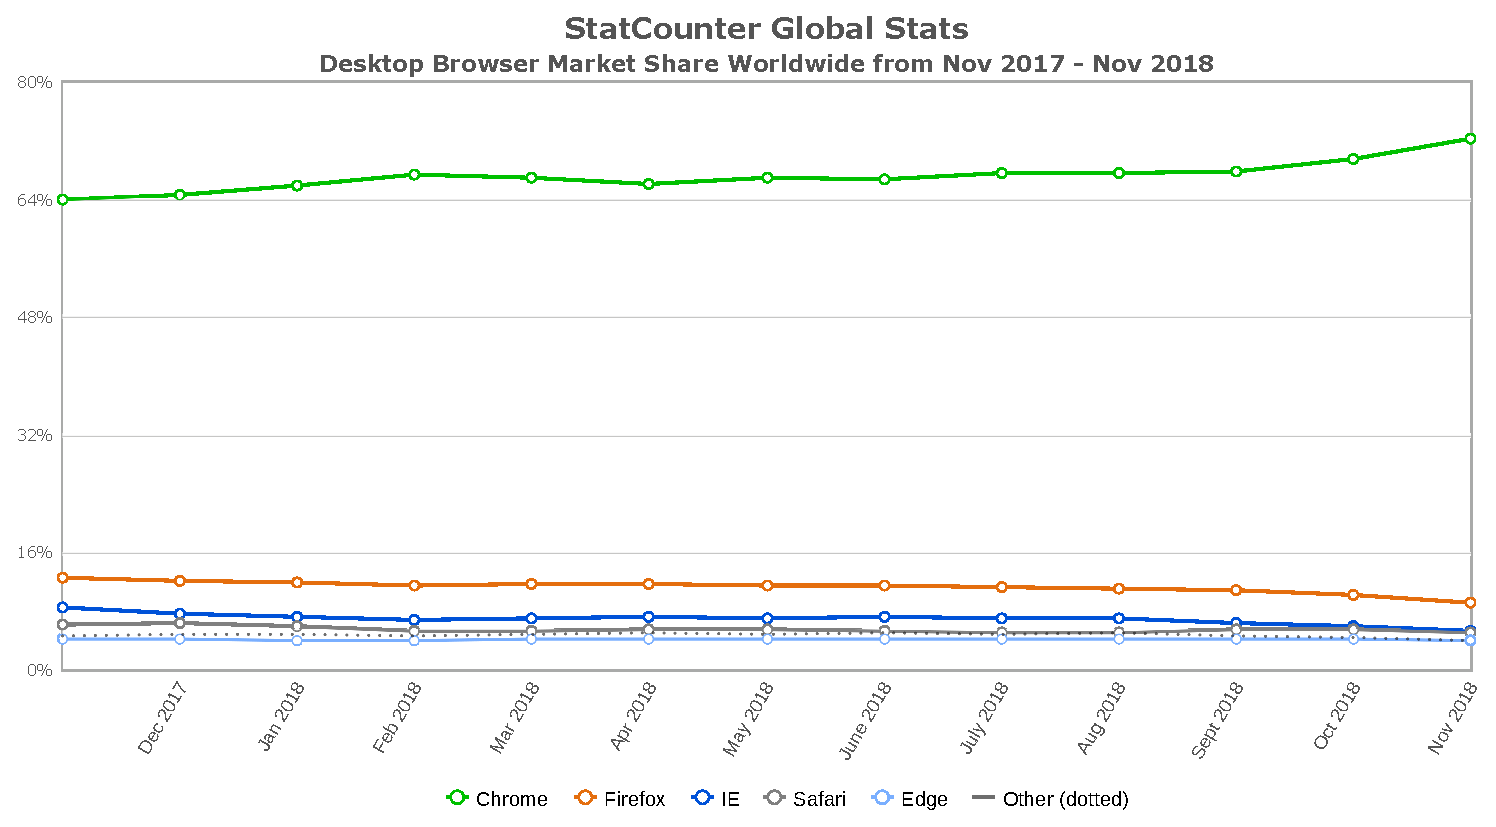
\includegraphics[width=1.0\textwidth]{graphics/compatibilidad.eps}
\caption{Participación de mercado de los navegadores hasta Noviembre del 2018.}
\label{software}
\source{http://gs.statcounter.com/browser-market-share/desktop/worldwide}
\end{figure}

Adicionalmente al uso del navegador \emph{Google Chrome} serán necesarios
otros navegadores para realizar la evaluación de compatibilidad sobre
vistas especificas del sistema, para este fin se consultó la información
disponible en la pagina de soporte provista por el fabricante, la cual como
puede verse en el \emph{cuadro \ref{soporte_navegadores}}, revela que se
soportan cinco navegadores diferentes bajo condiciones de limitación descritas
por el fabricante.

\begin{table}
\centering
\begin{tabular}{|p{6.0cm}|p{2.5cm}|p{1.4cm}|p{1.3cm}|p{1.3cm}|p{1.0cm}|}
\hline
& \footnotesize{\textbf{\emph{Microsoft Internet Explorer}}}
& \footnotesize{\textbf{\emph{Microsoft Edge}}}
& \footnotesize{\textbf{\emph{Google Chrome}}}
& \footnotesize{\textbf{\emph{Mozilla Firefox}}}
& \footnotesize{\textbf{\emph{Apple Safari}}} \\
\hline
\footnotesize{\emph{Lightning Experience}}
& \footnotesize{IE11 (EOL Diciembre 31, 2020)}
& \footnotesize{Ultima versión}
& \footnotesize{Ultima versión}
& \footnotesize{Ultima versión}
& \footnotesize{11.x+} \\
\footnotesize{\emph{Lightning Communities}}
& \footnotesize{IE11 (EOL Diciembre 31, 2020)}
& \footnotesize{Ultima versión}
& \footnotesize{Ultima versión}
& \footnotesize{Ultima versión}
& \footnotesize{11.x+} \\
\footnotesize{¿Consideraciones especiales de configuración?}
& \footnotesize{No}
& \footnotesize{No}
& \footnotesize{No}
& \footnotesize{No}
& \footnotesize{No} \\
\footnotesize{Limitaciones conocidas}
& \footnotesize{Sí}
& \footnotesize{Si}
& \footnotesize{No}
& \footnotesize{Si}
& \footnotesize{Si} \\
\hline
\end{tabular}
\caption{Lista de compatibilidad provista por \emph{Salesforce}.}
\label{soporte_navegadores}
\source{https://help.salesforce.com/articleView?id=getstart\_browsers\_sfx.htm}
\end{table}

\section{Planificación de actividades}
Para conseguir los objetivos planteados por el proyecto se realizarán las
actividades detalladas en el \emph{cuadro \ref{planificacion}} en la página
\pageref{planificacion}. Este cuadro detalla las actividades agrupadas por el
objetivo especifico y detallando también el resultado esperado de estas.

\begin{sidewaystable}
\renewcommand{\arraystretch}{1}
\linespread{1.25}
\centering
\small
\begin{tabular}{|l|l|p{6.5cm}|l|}
\hline
Objetivo General & Objetivos Específicos & Actividades & Resultados \\
\hline
\multirow{10}{4.0cm}{Implementar un \emph{framework} para la automatización de
las pruebas de interfaz de usuario en el módulo de Productos y Listas de Precios
en \emph{Salesforce}, para garantizar un procedimiento continuo de evaluación y
minimizar la cantidad de errores que contiene el software.} &
\multirow{3}{4.0cm}{Formular los casos de prueba necesarios que los módulos de
gestión de productos y listas de precios requieran para cubrir los atributos de
calidad requeridos.} &
Recolección de la información y exploración de los módulos específicos. &
\multirow{3}{4.0cm}{Casos de prueba para los módulos de Productos y Listas de
Precios.} \\
\cline{3-3}
& & Análisis y diseño de los tipos de evaluación requeridos para los módulos
específicos. & \\
\cline{3-3}
& & Formulación los casos de prueba necesarios para los módulos
específicos. & \\
\cline{2-4}
& \multirow{3}{4.0cm}{Diseñar e implementar los modelos y bibliotecas de
funciones que conforman un \emph{framework} de automatización.} &
Análisis y modelamiento de los componentes del \emph{framework}. &
\multirow{3}{4.0cm}{\emph{Framework} de automatización con los componentes
necesarios para la implementación de los casos de prueba.} \\
\cline{3-3}
& & Estructuración de los entornos de prueba y configuración de los servicios
disponibles. & \\
\cline{3-3}
& & Implementación de los componentes del \emph{framework}. & \\
\cline{2-4}
& \multirow{4}{4.0cm}{Automatizar los casos de prueba de las funciones que
componen la interfaz de usuario del módulo de gestión de productos y listas de
precios.} &
Implementación de los casos de prueba formulados. &
\multirow{4}{4.0cm}{Rutinas de automatización de los casos de prueba de los
módulos de Productos y Listas de Precios.} \\
\cline{3-3}
& & Implementación de pre condiciones y post condiciones en la ejecución de los
casos de prueba. & \\
\cline{3-3}
& & Ejecución de los casos de prueba automatizados. & \\
\cline{3-3}
& & Generación del reporte de resultados y reporte de errores. & \\
\hline
\end{tabular}
\caption{Planificación de actividades del proyecto.}
\label{planificacion}
\source{Elaboración propia.}
\end{sidewaystable}

\section{Elementos del producto}
Dentro del alcance de la evaluación se encuentran los componentes de productos
y listas de precios, las funcionalidades que comprenden estos se detallan en
esta sección, desde múltiples perspectivas de análisis.

Como se mencionó anteriormente, se consideró la interfaz
\emph{Lightning Experience}, como único objetivo de la evaluación. La versión
\emph{Lightning Experience} esta disponible para las siguientes ediciones del
producto: \emph{Essentials}, \emph{Group}, \emph{Professional},
\emph{Enterprise}, \emph{Performance}, \emph{Unlimited}, y \emph{Developer}.

\subsection{Productos}
El Producto para el software a evaluar, representa uno de los componentes
fundamentales y claves para el éxito, por ende es importante evaluarlo
desde múltiples facetas; la primera de estas es la funcionalidad provista por
las interfaces de este módulo. En la \emph{figura \ref{productos}} pueden verse
estas funcionalidades, clasificadas desde la perspectiva de la interfaz de
usuario.

Entre las funcionalidades que pueden apreciarse están las operaciones comunes
de creación, búsqueda, visualización, modificación, y eliminación de productos,
se omitieron las funcionalidades de controles de vista de lista, para que
todo este componente pueda ser tratado de manera separada. También pueden
observarse funciones relacionadas a registrar precios estándar y precios para
una lista de precios determinada.

En la \emph{figura \ref{productos_vistas}}, se aprecian las diferentes vistas
que comprenden el módulo, se resaltó con color amarillo aquellas vistas que son
de tipo formulario, mientras que se resaltó con color verde aquellas que son de
tipo confirmación de acción.

Además de las funcionalidades y vistas antes mencionadas, también se analizó el
comportamiento de los formularios que provee el módulo, como puede verse en la
\emph{figura \ref{productos_formularios}}.

\begin{figure}
\centering
\begin{tikzpicture}[
    grow via three points={one child at (0.5,-0.7) and
    two children at (0.5,-0.7) and (0.5,-1.4)},
    edge from parent path={(\tikzparentnode.south) |- (\tikzchildnode.west)}]
    \node {Productos}
        child { node {Nuevo}}
        child { node {Buscar: Producto}}
        child { node {Controles de Vista de Lista}
            child { node {\ldots}}
        }
        child [missing] {}
        child { node {Mostrar como}}
        child { node {Actualizar}}
        child { node {Filtrar por: Vista de Lista}}
        child { node {Modificar Lista}}
        child { node {Lista de Productos}
            child { node {Ver: Producto}
                child { node {Modificar}}
                child { node {Eliminar}}
                child { node {Duplicar}}
                child { node {Relacionado}
                    child { node {Agregar precio estándar}}
                    child { node {Agregar a lista de precios}}
                    child { node {Ver: Lista de precios}}
                    child { node {Modificar: Lista de precios}}
                    child { node {Eliminar: Lista de precios}}
                    child { node {Ver todos}
                        child { node {Actualizar}}
                    }
                }
                child [missing] {}
                child [missing] {}
                child [missing] {}
                child [missing] {}
                child [missing] {}
                child [missing] {}
                child [missing] {}
                child { node {Detalles}}
            }
            child [missing] {}
            child [missing] {}
            child [missing] {}
            child [missing] {}
            child [missing] {}
            child [missing] {}
            child [missing] {}
            child [missing] {}
            child [missing] {}
            child [missing] {}
            child [missing] {}
            child [missing] {}
            child { node {Modificar: Producto}}
            child { node {Eliminar: Producto}}
        };
\end{tikzpicture}
\caption{Funciones que componen el módulo de gestión de productos.}
\label{productos}
\source{Elaboración propia.}
\end{figure}

\begin{figure}
\centering
\begin{tikzpicture}[
    grow via three points={one child at (0.5,-0.7) and
    two children at (0.5,-0.7) and (0.5,-1.4)},
    edge from parent path={(\tikzparentnode.south) |- (\tikzchildnode.west)}]
    \node {Productos}
        child { node {Mostrar como}
            child { node {Tabla}}
            child { node {Kanban}}
        }
        child [missing] {}
        child [missing] {}
        child { node [form] {Crear Producto}}
        child { node {Filtros}}
        child { node {Producto}
            child { node [form] {Modificar: Producto}}
            child { node [confirm] {Eliminar: Producto}}
            child { node [form] {Crear Producto}}
            child { node {Detalles}}
            child { node {Relacionado}
                child { node [form] {Crear Entrada del catalogo de precios}}
                child { node [form] {Agregar a lista de precios}}
                child { node {Listas de precios}
                    child { node [form] {Modificar Entrada del catalogo de precios}}
                    child { node [confirm] {Eliminar entrada del catalogo de precios}}
                }
            }
        }
        child [missing] {}
        child [missing] {}
        child [missing] {}
        child [missing] {}
        child [missing] {}
        child [missing] {}
        child [missing] {}
        child [missing] {}
        child [missing] {}
        child [missing] {}
        child { node [form] {Modificar: Producto}}
        child { node [confirm] {Eliminar: Producto}};
\end{tikzpicture}
\caption{Vistas que componen el módulo de gestión de productos.}
\label{productos_vistas}
\source{Elaboración propia.}
\end{figure}

\begin{figure}
\centering
\begin{tikzpicture}[
    grow via three points={one child at (0.5,-0.7) and
    two children at (0.5,-0.7) and (0.5,-1.4)},
    edge from parent path={(\tikzparentnode.south) |- (\tikzchildnode.west)}]
    \node {Productos}
        child { node {Crear producto}
            child { node {Nombre del producto (*)}}
            child { node {Activo}}
            child { node {Código de producto}}
            child { node {Familia de productos}}
            child { node {Descripción del producto}}
        }
        child [missing] {}
        child [missing] {}
        child [missing] {}
        child [missing] {}
        child [missing] {}
        child { node {Crear entrada del catálogo de precios}
            child { node {Producto (*)}}
            child { node {Activo}}
            child { node {Lista de precios (*)}}
            child { node {Precio de la lista (*)}}
            child { node {Utilizar precio estándar}}
        }
        child [missing] {}
        child [missing] {}
        child [missing] {}
        child [missing] {}
        child [missing] {}
        child { node {Agregar a lista de precios}
            child { node {Lista de precios (*)}}
            child { node {Divisa (*)}}
        }
        child [missing] {}
        child [missing] {}
        child { node {Modificar entrada del catálogo de precios}
            child { node {Activo}}
            child { node {Precio de la lista (*)}}
            child { node {Utilizar precio estándar}}
        };
\end{tikzpicture}
\caption{Formularios que componen el módulo de gestión de productos.}
\label{productos_formularios}
\source{Elaboración propia.}
\end{figure}

\subsection{Listas de Precios}
Las Listas de Precios, tienen como objetivo, hacer que un mismo producto pueda
tener múltiples precios, dependiendo de como la organización cliente maneje sus
canales de distribución y producción. Al igual que en el módulo de productos, en
la \emph{figura \ref{listas_de_precios}} pueden verse las funcionalidades
clasificadas desde la perspectiva de la interfaz de usuario, también se omitió
la sección de los controles de vista de lista.

Las funciones de Listas de Precios son muy similares a aquellas vistas en el
módulo de productos, analizado anteriormente.

En la \emph{figura \ref{listas_de_precios_vistas}}, se detallan aquellas vistas
presentes en este módulo, de la misma manera se ha destacado con amarillo a
aquellas vistas que son formularios, mientras que en verde se presentan a
aquellas que representan diálogos de confirmación.

También de las funcionalidades y vistas antes mencionadas, se analizó el
comportamiento de los formularios que provee este módulo, como puede verse en la
\emph{figura \ref{listas_de_precios_formularios}}.

\begin{figure}
\centering
\begin{tikzpicture}[
    grow via three points={one child at (0.5,-0.7) and
    two children at (0.5,-0.7) and (0.5,-1.4)},
    edge from parent path={(\tikzparentnode.south) |- (\tikzchildnode.west)}]
    \node {Listas de Precios}
        child { node {Nuevo}}
        child { node {Buscar: Lista de precios}}
        child { node {Controles de Vista de Lista}
            child { node {\ldots}}
        }
        child [missing] {}
        child { node {Mostrar como}}
        child { node {Actualizar}}
        child { node {Filtrar por: Vista de Lista}}
        child { node {Modificar Lista}}
        child { node {Lista de Listas de Precios}
            child { node {Ver: Lista de precios}
                child { node {Modificar}}
                child { node {Eliminar}}
                child { node {Duplicar}}
                child { node {Relacionado}
                    child { node {Agregar productos}}
                    child { node {Ver: Producto}}
                    child { node {Modificar: Producto}}
                    child { node {Eliminar: Producto}}
                    child { node {Ver todos}
                        child { node {Actualizar}}
                    }
                    child [missing] {}
                    child { node {Historial de lista de precios (Ver todos)}
                        child { node {Actualizar}}
                    }
                }
                child [missing] {}
                child [missing] {}
                child [missing] {}
                child [missing] {}
                child [missing] {}
                child [missing] {}
                child [missing] {}
                child [missing] {}
                child { node {Detalles}}
            }
            child [missing] {}
            child [missing] {}
            child [missing] {}
            child [missing] {}
            child [missing] {}
            child [missing] {}
            child [missing] {}
            child [missing] {}
            child [missing] {}
            child [missing] {}
            child [missing] {}
            child [missing] {}
            child [missing] {}
            child { node {Modificar: Lista de Precios}}
            child { node {Eliminar: Lista de Precios}}
        };
\end{tikzpicture}
\caption{Funciones que componen el módulo de gestión de listas de precios.}
\label{listas_de_precios}
\source{Elaboración propia.}
\end{figure}

\begin{figure}
\centering
\begin{tikzpicture}[
    grow via three points={one child at (0.5,-0.7) and
    two children at (0.5,-0.7) and (0.5,-1.4)},
    edge from parent path={(\tikzparentnode.south) |- (\tikzchildnode.west)}]
    \node {Listas de Precios}
        child { node {Mostrar como}
            child { node {Tabla}}
            child { node {Kanban}}
        }
        child [missing] {}
        child [missing] {}
        child { node [form] {Crear Lista de precios}}
        child { node {Filtros}}
        child { node {Lista de precios}
            child { node [form] {Modificar: Lista de Precios}}
            child { node [form] {Crear Lista de precios}}
            child { node [confirm] {Eliminar: Lista de precios}}
            child { node {Detalles}}
            child { node {Relacionado}
                child { node [form] {Agregar productos}
                    child { node [form] {Modificar Entrada del catalogo de precios}}
                }
                child [missing] {}
                child { node {Productos}
                    child { node [form] {Modificar Entrada del catalogo de precios}}
                    child { node [confirm] {Eliminar Entrada del catalogo de precios}}
                }
                child [missing] {}
                child [missing] {}
                child { node {Historial de lista de precios}}
            }
        }
        child [missing] {}
        child [missing] {}
        child [missing] {}
        child [missing] {}
        child [missing] {}
        child [missing] {}
        child [missing] {}
        child [missing] {}
        child [missing] {}
        child [missing] {}
        child [missing] {}
        child { node [form] {Modificar: Lista de Precio}}
        child { node [confirm] {Eliminar: Lista de Precio}};
\end{tikzpicture}
\caption{Vistas que componen el módulo de gestión de listas de precios.}
\label{listas_de_precios_vistas}
\source{Elaboración propia.}
\end{figure}

\begin{figure}
\centering
\begin{tikzpicture}[
    grow via three points={one child at (0.5,-0.7) and
    two children at (0.5,-0.7) and (0.5,-1.4)},
    edge from parent path={(\tikzparentnode.south) |- (\tikzchildnode.west)}]
    \node {Listas de Precios}
        child { node {Crear lista de precios}
            child { node {Nombre de la lista de precios (*)}}
            child { node {Activo}}
            child { node {Descripción}}
            child { node {Es lista de precios estándar}}
        }
        child [missing] {}
        child [missing] {}
        child [missing] {}
        child [missing] {}
        child { node {Agregar productos}
            child { node {Buscar entrada de catálogos de precios}
                child { node {Modificar Entrada de catálogos de precios}}
            }
        };
\end{tikzpicture}
\caption{Formularios que componen el módulo de gestión de listas de precios.}
\label{listas_de_precios_formularios}
\source{Elaboración propia.}
\end{figure}

\subsection{Controles de Vista de Lista}
Los Controles de Vista de Lista son funcionalidades equivalentes entre los 
dos componentes que están siendo evaluados, por lo que se ha decidido realizar
un análisis separado de estos. En la \emph{figura \ref{vista_de_lista}} puede
verse las funciones omitidas en los diagramas anteriores relativas a los
controles de vista.

En la \emph{figura \ref{vista_de_lista_vistas}}, se detallan aquellas vistas
provistas por este componente, de la misma manera que en los dos módulos
anteriormente citados, aquí también se han destacado con amarillo a
aquellas vistas que son formularios, mientras que en verde se presentan a
aquellas que representan diálogos de confirmación.

También de las funcionalidades y vistas antes mencionadas, se analizó el
comportamiento de los formularios que provee este módulo, como puede verse en la
\emph{figura \ref{vista_de_lista_formularios}}.

\begin{figure}
\centering
\begin{tikzpicture}[
    grow via three points={one child at (0.5,-0.7) and
    two children at (0.5,-0.7) and (0.5,-1.4)},
    edge from parent path={(\tikzparentnode.south) |- (\tikzchildnode.west)}]
    \node {Controles de Vista de Lista}
        child { node {Nuevo}}
        child { node {Duplicar}}
        child { node {Cambiar nombre}}
        child { node {Configuración de colaboración}
            child { node {Modificar}}
        }
        child [missing] {}
        child { node {Modificar filtros de lista}
            child { node {Ver/Modificar: Filtro}}
            child { node {Eliminar: Filtro}}
            child { node {Agregar Filtro}}
            child { node {Eliminar todos}}
            child { node {Agregar lógica de filtro}}
        }
        child [missing] {}
        child [missing] {}
        child [missing] {}
        child [missing] {}
        child [missing] {}
        child { node {Seleccionar los campos que se visualizaran}}
        child { node {Eliminar}}
        child { node {Restablecer anchuras de columna}}
        child { node {Configuración de Kanban}};
\end{tikzpicture}
\caption{Funciones que componen el módulo de gestión de vistas de lista.}
\label{vista_de_lista}
\source{Elaboración propia.}
\end{figure}

\begin{figure}[H]
\centering
\begin{tikzpicture}[
    grow via three points={one child at (0.5,-0.7) and
    two children at (0.5,-0.7) and (0.5,-1.4)},
    edge from parent path={(\tikzparentnode.south) |- (\tikzchildnode.west)}]
    \node {Vista de Lista}
        child { node [form] {Nueva vista de lista}}
        child { node [form] {Duplicar vista de lista}}
        child { node [form] {Cambiar nombre}}
        child { node [form] {Configuración de colaboración}}
        child { node [form] {Seleccionar los campos que se visualizaran}}
        child { node [confirm] {Eliminar}}
        child { node [form] {Configuración de Kanban}};
\end{tikzpicture}
\caption{Vistas que componen el módulo de gestión de listas de precios.}
\label{vista_de_lista_vistas}
\source{Elaboración propia.}
\end{figure}

\begin{figure}
\centering
\begin{tikzpicture}[
    grow via three points={one child at (0.5,-0.7) and
    two children at (0.5,-0.7) and (0.5,-1.4)},
    edge from parent path={(\tikzparentnode.south) |- (\tikzchildnode.west)}]
    \node {Vista de lista}
        child { node {Nueva vista de lista}
            child { node {Nombre de la lista (*)}}
            child { node {List API Name (*)}}
            child { node {¿Quien ve esta vista de lista?}
                child { node {Solo yo puedo ver esta vista de lista}}
                child { node {Todos los usuarios pueden ver esta vista de lista}}
                child { node {Compartir vista de lista con grupos de usuarios}}
            }
        }
        child [missing] {}
        child [missing] {}
        child [missing] {}
        child [missing] {}
        child [missing] {}
        child [missing] {}
        child { node {Cambiar nombre}
            child { node {Nombre de lista (*)}}
        }
        child [missing] {}
        child { node {Configuración de colaboración}
            child { node {¿Quien ve esta vista de lista?}
                child { node {Solo yo puedo ver esta vista de lista}}
                child { node {Todos los usuarios pueden ver esta vista de lista}}
                child { node {Compartir vista de lista con grupos de usuarios}}
            }
        }
        child [missing] {}
        child [missing] {}
        child [missing] {}
        child [missing] {}
        child { node {Agregar filtro}
            child { node {Campo}}
            child { node {Operador}}
            child { node {Valor}}
        }
        child [missing] {}
        child [missing] {}
        child [missing] {}
        child { node {Agregar lógica de filtro}
            child { node {Lógica de filtro}}
        }
        child [missing] {}
        child { node {Seleccionar los campos que se visualizaran}
            child { node {Campos disponibles}}
            child { node {Campos visibles (*)}}
        }
        child [missing] {}
        child [missing] {}
        child { node {Configuración de Kanban}
            child { node {Resumir por)}}
            child { node {Agrupar por (*)}}
        };
\end{tikzpicture}
\caption{Formularios que componen el módulo de gestión de vistas de listas.}
\label{vista_de_lista_formularios}
\source{Elaboración propia.}
\end{figure}

\section{Análisis de valor limite}
Para el análisis de los formularios se crearon las respectivas tablas producidas
a partir del análisis de sus valores limite, las cuales son descritas a
continuación:

\begin{itemize}
    \item Crear Producto, que puede verse en el \emph{cuadro \ref{myers_01}}.
    \item Crear Entrada del catalogo de precios, que puede verse en el
        \emph{cuadro \ref{myers_02}}.
    \item Agregar a lista de precios, que puede verse en el
        \emph{cuadro \ref{myers_03}}.
    \item Modificar Entrada del catalogo de precios, que puede verse en el
        \emph{cuadro \ref{myers_04}}.
    \item Crear Lista de precios, que puede verse en el
        \emph{cuadro \ref{myers_05}}.
    \item Agregar productos, que puede verse en el \emph{cuadro \ref{myers_06}}.
    \item Nueva vista de lista, que puede verse en el
        \emph{cuadro \ref{myers_07}}.
    \item Cambiar nombre, que puede verse en el \emph{cuadro \ref{myers_08}}.
    \item Configuración de colaboración, que puede verse en el
        \emph{cuadro \ref{myers_09}}.
\end{itemize}

\begin{table}
\centering
\begin{tabular}{|p{6.0cm}|l|l|l|}
\hline
\footnotesize{\textbf{Variable}} & \footnotesize{\textbf{Casos Posibles}} & \footnotesize{\textbf{Casos Inválidos}} & \footnotesize{\textbf{Limites}} \\
\hline
\footnotesize{Nombre del producto} & \footnotesize{[1-255] caracteres} & & \footnotesize{0} \\
& & \footnotesize{0} & \footnotesize{1} \\
& & \footnotesize{$>$255} & \footnotesize{255} \\
& & & \footnotesize{256} \\
\hline
\footnotesize{Activo} & \footnotesize{\{verdadero,falso\}} & & \\
\hline
\footnotesize{Código de producto} & \footnotesize{[0-255] caracteres} & & \footnotesize{0} \\
& & \footnotesize{$>$255} & \footnotesize{255} \\
& & & \footnotesize{256} \\
\hline
\footnotesize{Familia de productos} & \footnotesize{ninguno,[lista de valores]} & & \\
\hline
\footnotesize{Programación de cantidades activada} & \footnotesize{\{verdadero,falso\}} & & \\
\hline
\footnotesize{Programación de ingresos activada} & \footnotesize{\{verdadero,falso\}} & & \\
\hline
\footnotesize{Descripción del producto} & \footnotesize{[0,4000] caracteres} & & \footnotesize{0} \\
& & \footnotesize{$>$4000} & \footnotesize{4000} \\
& & & \footnotesize{4001} \\
\hline
\end{tabular}
\caption{Análisis de valor limite para el formulario «Crear Producto»}
\label{myers_01}
\source{Elaboración propia.}
\end{table}

\begin{table}
\centering
\begin{tabular}{|p{3.0cm}|p{4.0cm}|p{4.0cm}|l|}
\hline
\footnotesize{\textbf{Variable}} & \footnotesize{\textbf{Casos Posibles}} & \footnotesize{\textbf{Casos Inválidos}} & \footnotesize{\textbf{Limites}} \\
\hline
\footnotesize{Producto} & \footnotesize{[lista de valores]} & & \\
\hline
\footnotesize{Activo}  & \footnotesize{\{verdadero,falso\}} & & \\
\hline
\footnotesize{Lista de precios} & \footnotesize{[lista de valores]} & & \\
\hline
\footnotesize{Precio de la lista} & \footnotesize{[} & \footnotesize{$<$-9.007.199.254.740.991} & \footnotesize{-9.007.199.254.740.992} \\
& \footnotesize{-9.007.199.254.740.991} & & \footnotesize{-9.007.199.254.740.991} \\
& \footnotesize{9.007.199.254.740.991} & & \footnotesize{9.007.199.254.740.991} \\
& \footnotesize{]} & \footnotesize{$>$9.007.199.254.740.991} & \footnotesize{9.007.199.254.740.992} \\
& \footnotesize{3 decimales} & & \footnotesize{0,999} \\
& & \footnotesize{4 decimales} & \footnotesize{0,9999} \\
\hline
\footnotesize{Utilizar Precio estándar} & \footnotesize{\{verdadero,falso\}} & & \\
\hline
\end{tabular}
\caption{Análisis de valor limite para el formulario «Crear Entrada del catalogo de precios»}
\label{myers_02}
\source{Elaboración propia.}
\end{table}

\begin{table}
\centering
\begin{tabular}{|p{6.0cm}|l|l|l|}
\hline
\footnotesize{\textbf{Variable}} & \footnotesize{\textbf{Casos Posibles}} & \footnotesize{\textbf{Casos Inválidos}} & \footnotesize{\textbf{Limites}} \\
\hline
\footnotesize{Lista de precios} & \footnotesize{ninguno,[lista de valores]} & & \\
\hline
\footnotesize{Divisa} & \footnotesize{ninguno,[lista de valores]} & & \\
\hline
\end{tabular}
\caption{Análisis de valor limite para el formulario «Agregar a lista de precios»}
\label{myers_03}
\source{Elaboración propia.}
\end{table}

\begin{table}
\centering
\begin{tabular}{|p{3.0cm}|p{4.0cm}|p{4.0cm}|l|}
\hline
\footnotesize{\textbf{Variable}} & \footnotesize{\textbf{Casos Posibles}} & \footnotesize{\textbf{Casos Inválidos}} & \footnotesize{\textbf{Limites}} \\
\hline
\footnotesize{Activo} & \footnotesize{\{verdadero,falso\}} & & \\
\hline
\footnotesize{Precio de la lista} & \footnotesize{[} & \footnotesize{$<$-9.007.199.254.740.991} & \footnotesize{-9.007.199.254.740.992} \\
& \footnotesize{-9.007.199.254.740.991} & & \footnotesize{-9.007.199.254.740.991} \\
& \footnotesize{9.007.199.254.740.991} & & \footnotesize{9.007.199.254.740.991} \\
& \footnotesize{]} & \footnotesize{$>$9.007.199.254.740.991} & \footnotesize{9.007.199.254.740.992} \\
& \footnotesize{3 decimales} & & \footnotesize{0,999} \\
& & \footnotesize{4 decimales} & \footnotesize{0,9999} \\
\hline
\footnotesize{Utilizar precio estándar} & \footnotesize{\{verdadero,falso\}} & & \\
\hline
\end{tabular}
\caption{Análisis de valor limite para el formulario «Modificar Entrada del catalogo de precios»}
\label{myers_04}
\source{Elaboración propia.}
\end{table}

\begin{table}
\centering
\begin{tabular}{|p{6.0cm}|l|l|l|}
\hline
\footnotesize{\textbf{Variable}} & \footnotesize{\textbf{Casos Posibles}} & \footnotesize{\textbf{Casos Inválidos}} & \footnotesize{\textbf{Limites}} \\
\hline
\footnotesize{Nombre de la lista de precios} & \footnotesize{[1-255] caracteres} & & \footnotesize{0} \\
& & \footnotesize{0} & \footnotesize{1} \\
& & \footnotesize{$>$255} & \footnotesize{255} \\
& & & \footnotesize{256} \\
\hline
\footnotesize{Activo} & \footnotesize{\{verdadero,falso\}} & & \\
\hline
\footnotesize{Descripción del producto} & \footnotesize{[0,255] caracteres} & & \footnotesize{0} \\
& & \footnotesize{$>$255} & \footnotesize{255} \\
& & & \footnotesize{256} \\
\hline
\footnotesize{Es lista de precios estándar} & \footnotesize{\{verdadero,falso\}} & & \\
\hline
\end{tabular}
\caption{Análisis de valor limite para el formulario «Crear Lista de precios»}
\label{myers_05}
\source{Elaboración propia.}
\end{table}

\begin{table}
\centering
\begin{tabular}{|p{3.0cm}|p{4.0cm}|p{4.0cm}|l|}
\hline
\footnotesize{\textbf{Variable}} & \footnotesize{\textbf{Casos Posibles}} & \footnotesize{\textbf{Casos Inválidos}} & \footnotesize{\textbf{Limites}} \\
\hline
\footnotesize{Buscar Entrada de catálogos de precios\ldots} & \footnotesize{[1-500] caracteres} & & \footnotesize{0} \\
& & & \footnotesize{1} \\
& & & \footnotesize{500} \\
& & & \footnotesize{501} \\
\hline
\multicolumn{4}{|l|}{\footnotesize{Modificar Entrada de catálogos de precios seleccionada}} \\
\hline
\footnotesize{Activo} & \footnotesize{\{verdadero,falso\}} & & \\
\hline
\footnotesize{Precio de la lista} & \footnotesize{[} & \footnotesize{$<$-9.007.199.254.740.991} & \footnotesize{-9.007.199.254.740.992} \\
& \footnotesize{-9.007.199.254.740.991} & & \footnotesize{-9.007.199.254.740.991} \\
& \footnotesize{9.007.199.254.740.991} & & \footnotesize{9.007.199.254.740.991} \\
& \footnotesize{]} & \footnotesize{$>$9.007.199.254.740.991} & \footnotesize{9.007.199.254.740.992} \\
& \footnotesize{3 decimales} & & \footnotesize{0,999} \\
& & \footnotesize{4 decimales} & \footnotesize{0,9999} \\
\hline
\footnotesize{Utilizar Precio estándar} & \footnotesize{\{verdadero,falso\}} & & \\
\hline
\end{tabular}
\caption{Análisis de valor limite para el formulario «Agregar productos»}
\label{myers_06}
\source{Elaboración propia.}
\end{table}

\begin{table}
\centering
\begin{tabular}{|p{3.0cm}|p{7.0cm}|p{3.0cm}|l|}
\hline
\footnotesize{\textbf{Variable}} & \footnotesize{\textbf{Casos Posibles}} & \footnotesize{\textbf{Casos Inválidos}} & \footnotesize{\textbf{Limites}} \\
\hline
\footnotesize{Nombre de lista} & \footnotesize{[1-40] caracteres} & & \footnotesize{0} \\
& & \footnotesize{0} & \footnotesize{1} \\
& & \footnotesize{$>$40} & \footnotesize{40} \\
& & & \footnotesize{41} \\
\hline
\footnotesize{List API Name} & \footnotesize{[1-80]} & & \footnotesize{0} \\
& & \footnotesize{0} & \footnotesize{1} \\
& & \footnotesize{$>$80} & \footnotesize{80} \\
& & & \footnotesize{81} \\
& \footnotesize{[a-zA-Z][a-zA-Z0-9\_][a-zA-Z0-9]} & & \\
& & \footnotesize{1xxxxx} & \footnotesize{1xxxxx} \\
& & \footnotesize{\_xxxxx} & \footnotesize{\_xxxxx} \\
& & \footnotesize{xxx\_\_xxx} & \footnotesize{xxx\_\_xxx} \\
& & \footnotesize{xxxxx\_} & \footnotesize{xxxxx\_} \\
\hline
\footnotesize{¿Quien ve esta lista?} & \footnotesize{Solo yo puedo ver esta vista de lista} & & \\
& \footnotesize{Todos los usuarios pueden ver esta vista de lista} & & \\
& \footnotesize{Compartir vista de lista con grupos de usuarios} & & \\
\hline
\end{tabular}
\caption{Análisis de valor limite para el formulario «Nueva vista de lista»}
\label{myers_07}
\source{Elaboración propia.}
\end{table}

\begin{table}
\centering
\begin{tabular}{|l|l|l|l|}
\hline
\footnotesize{\textbf{Variable}} & \footnotesize{\textbf{Casos Posibles}} & \footnotesize{\textbf{Casos Inválidos}} & \footnotesize{\textbf{Limites}} \\
\hline
\footnotesize{Nombre de lista} & \footnotesize{[1-40] caracteres} & & \footnotesize{0} \\
& & \footnotesize{0} & \footnotesize{1} \\
& & \footnotesize{$>$40} & \footnotesize{40} \\
& & & \footnotesize{41} \\
\hline
\end{tabular}
\caption{Análisis de valor limite para el formulario «Cambiar nombre»}
\label{myers_08}
\source{Elaboración propia.}
\end{table}

\begin{table}
\centering
\begin{tabular}{|l|l|l|l|}
\hline
\footnotesize{\textbf{Variable}} & \footnotesize{\textbf{Casos Posibles}} & \footnotesize{\textbf{Casos Inválidos}} & \footnotesize{\textbf{Limites}} \\
\hline
\footnotesize{¿Quien ve esta lista?} & \footnotesize{Solo yo puedo ver esta vista de lista} & & \\
& \footnotesize{Todos los usuarios pueden ver esta vista de lista} & & \\
& \footnotesize{Compartir vista de lista con grupos de usuarios} & & \\
\hline
\end{tabular}
\caption{Análisis de valor limite para el formulario «Configuración de colaboración»}
\label{myers_09}
\source{Elaboración propia.}
\end{table}

\section{Casos de prueba}
A partir del análisis realizado, se terminó formulando múltiples casos de
prueba, estos se encuentran descritos en el \emph{\textbf{apéndice
\ref{appendix_testscases}}} categorizados e individualizados según el área y
subarea al que pertenecen.

En la \emph{figura \ref{tc-tests}}, se puede ver la distribución de los casos de
prueba según el tipo de evaluación realizado, puede apreciarse que las pruebas
funcionales ocupan mas de la mitad de la totalidad de casos de prueba en el
proyecto, mientras que los casos de prueba negativos, y de aceptación, están más
próximos al 10\%.

En la \emph{figura \ref{tc-type}}, se puede ver la distribución de los casos de
prueba según el tipo de acción que se realiza en el sistema, es decir, si son
casos que afectan la interfaz de usuario, si mas bien son funciones de
validación, o si realizan alguna petición al servidor, sea esta de lectura o
escritura.

Puede apreciarse igualmente que la mayor parte de los casos de prueba están
orientados a evaluar el comportamiento de la interfaz de usuario, mientras que
en un 25\% aproximadamente se evalúan funcionalidades que se comunican con el
servidor.

\begin{figure}
\centering
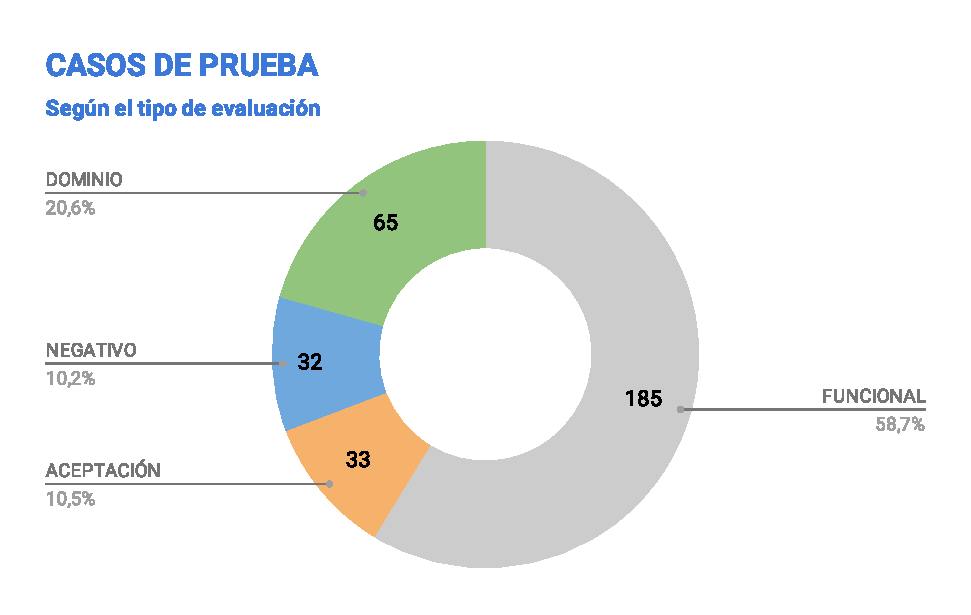
\includegraphics[width=1.0\textwidth]{graphics/tc-tests.eps}
\caption{Casos de Prueba según el tipo de evaluación realizada.}
\label{tc-tests}
\source{Elaboración propia.}
\end{figure}

\begin{figure}
\centering
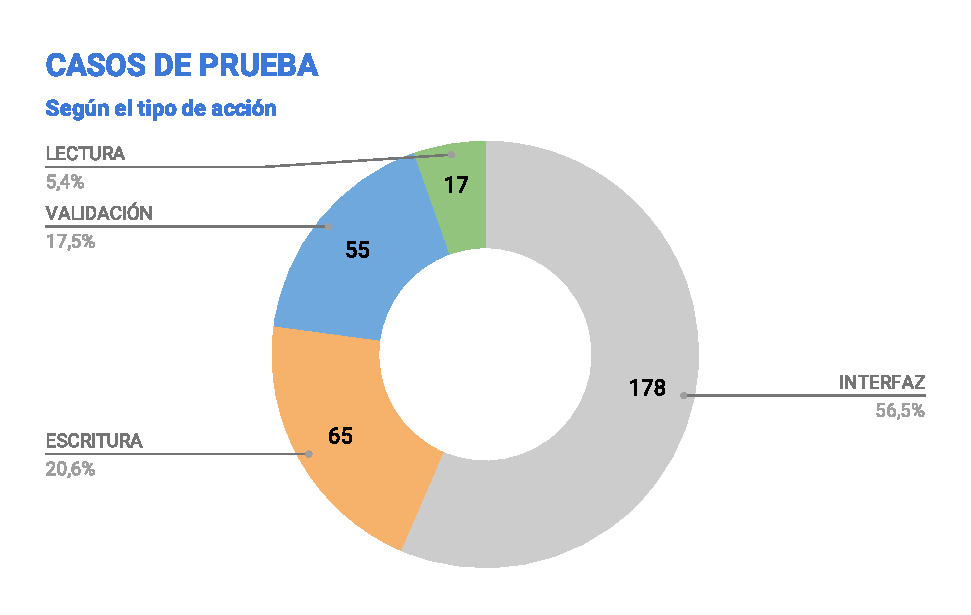
\includegraphics[width=1.0\textwidth]{graphics/tc-type.eps}
\caption{Casos de Prueba según el tipo de acción a evaluar.}
\label{tc-type}
\source{Elaboración propia.}
\end{figure}


\chapter{Conclusiones}

\section{Resultados}
En la figura \ref{tc-tests}, se puede ver la distribución de los casos de prueba
según el tipo de evaluación realizado, puede apreciarse que las pruebas
funcionales ocupan mas de la mitad de la totalidad de casos de prueba en el
proyecto, mientras que los casos de prueba negativos, y de aceptación, están más
próximos al 10\%.

\begin{figure}
\centering
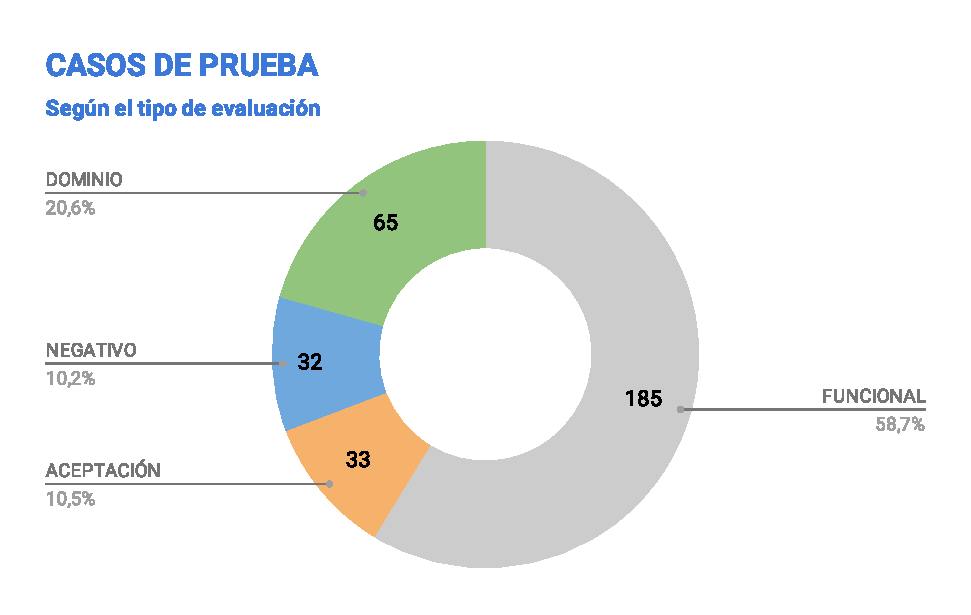
\includegraphics[width=1.0\textwidth]{graphics/tc-tests.eps}
\caption{Casos de Prueba según el tipo de evaluación realizada.}
\label{tc-tests}
\end{figure}

En la figura \ref{tc-type}, se puede ver la distribución de los casos de prueba
según el tipo de acción que se realiza en el sistema, es decir, si son casos
que afectan la interfaz de usuario, si mas bien son funciones de validación, o
si realizan alguna petición al servidor, sea esta de lectura o escritura.

Puede apreciarse igualmente que la mayor parte de los casos de prueba están
orientados a evaluar el comportamiento de la interfaz de usuario, mientras que
en un 25\% aproximadamente se evalúan funcionalidades que se comunican con el
servidor.

\begin{figure}
\centering
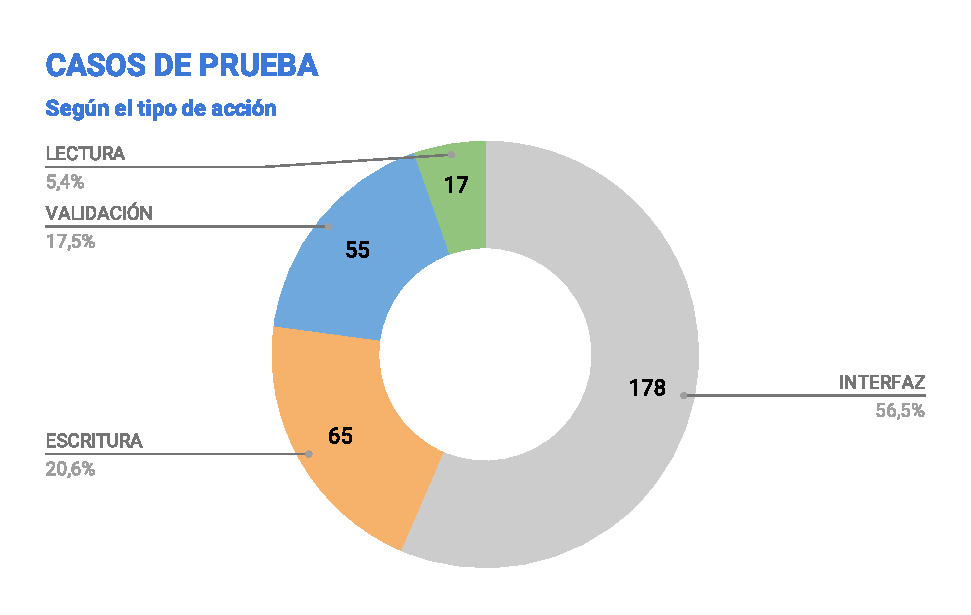
\includegraphics[width=1.0\textwidth]{graphics/tc-type.eps}
\caption{Casos de Prueba según el tipo de acción a evaluar.}
\label{tc-type}
\end{figure}

En las figuras \ref{results-tests} y \ref{results-type}, se condensan los
resultados obtenidos de la ejecución de los casos de prueba, en los cuales
únicamente fallaron 2 casos de prueba, ambos relacionados a un mismo formulario,
como puede verse en el reporte de error adjunto, y debido al fallo de estos
también se bloquearon dos casos de prueba.

\begin{figure}
\centering
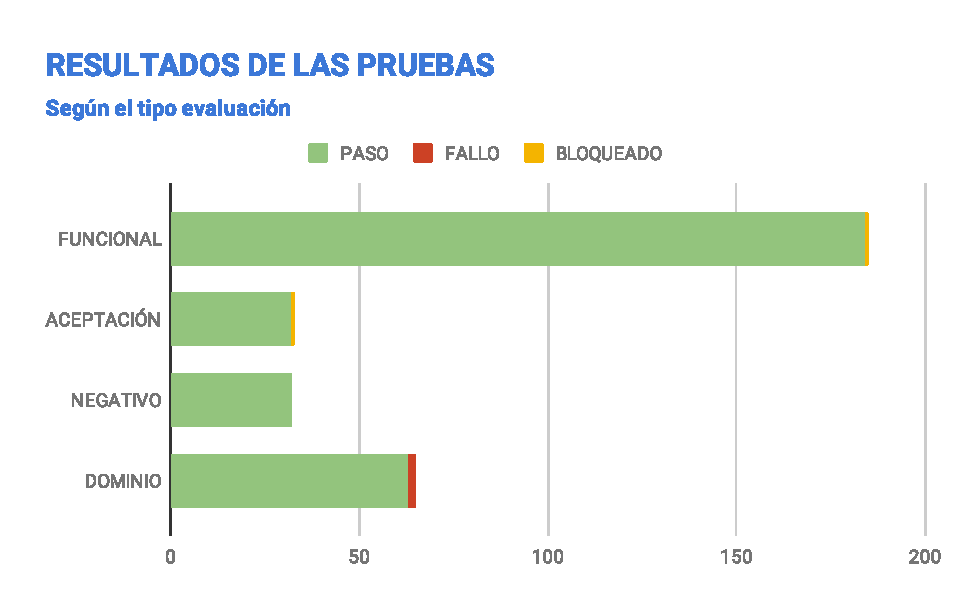
\includegraphics[width=1.0\textwidth]{graphics/results-tests.eps}
\caption{Resultados de las pruebas clasificadas por tipo de evaluación.}
\label{results-tests}
\end{figure}

\begin{figure}
\centering
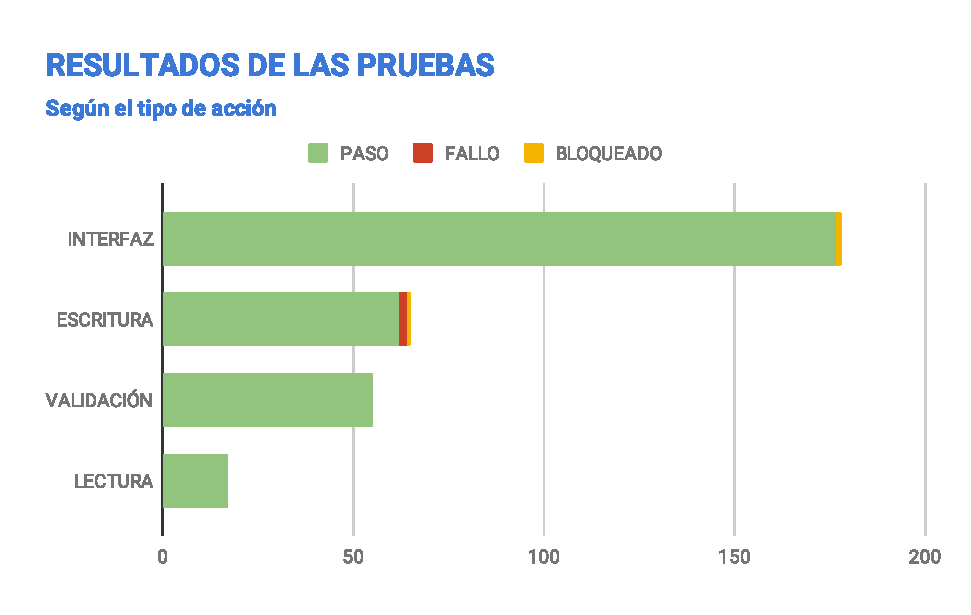
\includegraphics[width=1.0\textwidth]{graphics/results-type.eps}
\caption{Resultados de las pruebas clasificadas por tipo de acción a evaluar.}
\label{results-type}
\end{figure}

Presentados los resultados de la ejecución de las pruebas, vemos que de los 315
casos de pruebas únicamente existes 2 bloqueados, y dos fallidos. Por ende se
tiene 98.74\% de casos de prueba exitosos, lo que lleva a concluir que los
atributos de calidad esperados del sistema están cubiertos por completo.


\chapter{Conclusiones y Recomendaciones}

Este capítulo compendia la conclusión misma del proyecto, para finalizar
presentando las recomendaciones finales que se han planteado a partir de los
resultados obtenidos.

\section{Conclusiones}
Todos los objetivos fueron cubiertos correctamente, como se describen a
continuación:

\begin{itemize}
\item El \textbf{primer objetivo} (Formular los casos de prueba necesarios que
los módulos de gestión de productos y listas de precios requieran para cubrir
los atributos de calidad requeridos) ha sido alcanzado, ya que se consiguió un
buen grado de cobertura tanto del modulo de productos, como del modulo de listas
de precios con los casos de prueba planteados, y categorizando apropiadamente
según el uso apropiado que requiera, ya sea para la ejecución de una prueba de
regresión, una de aceptación o la evaluación total del software.
\item El \textbf{segundo objetivo} (Diseñar e implementar los modelos y
bibliotecas de funciones que conforman un \emph{framework} de automatización)
ha sido cubierto, ya que el \emph{framework} de automatización esta utilizando
los patrones de diseño apropiados, e implementados con una biblioteca de
automatización ampliamente utilizada, haciendo que pueda ser fácilmente
mantenible, usable y extensible.
\item El \textbf{tercer objetivo} (Automatizar los casos de prueba de las
funciones que componen la interfaz de usuario del módulo de gestión de productos
y listas de precios) ha sido cubierto, ya que se tienen implementados los casos
de prueba planteados.
\end{itemize}

Con lo que se puede concluir que el objetivo general \textbf{ha sido cumplido},
al haber completado la creación del \emph{framework} y ya que el procedimiento
de evaluación del modulo de Productos y Listas de Precio ahora puede hacerse de
forma continua y acomodándose a diferentes etapas del desarrollo del software,
minimizando la cantidad de posibles errores y mejorando la calidad general del
sistema.

\section{Recomendaciones}
Si bien se han cubierto las pruebas funcionales, además de realizarse pruebas
de dominio para los formularios y pruebas negativas para los mensajes de error,
se cree necesario extender para incluir dos tipos de pruebas que podrían ser
muy útiles para el software a evaluar.

\begin{itemize}
\item Pruebas de localización (l10n).
\item Pruebas de internacionalización (i18n).
\end{itemize}

Ambas muy necesarias para un software con soporte para múltiples idiomas,
culturas y formatos diversos.



\printbibliography[
heading=bibintoc,
title={Bibliografía}
]

\begin{appendix}
\chapter{Baterías de casos de pruebas}
Este anexo tiene como objetivo mostrar cada caso de prueba evaluado clasificado
por el tipo de test que ha sido ejecutado y el tipo de acción que se esta
evaluando.

Para estas la compresión de las tablas es necesario tener en cuanta las
siguientes abreviaturas:

\begin{itemize}
    \item P, hace referencia al modulo de Productos.
    \item LP, hace referencia al modulo de Listas de Precios.
    \item VL, hace referencia al componente de Vistas de Lista.
    \item A00x, es el modelo de ID para un caso de prueba de tipo aceptación.
    \item F00x, es el modelo de ID para un caso de prueba de tipo funcional.
    \item D00x, es el modelo de ID para un caso de prueba de tipo dominio.
    \item N00x, es el modelo de ID para un caso de prueba de tipo negativo.
\end{itemize}

\section{Bateria de Pruebas}

\begin{landscape}
\centering
\small
\begin{longtable}[htb]{|l|l|p{5.0cm}|p{13.0cm}|}
\hline
\textbf{ID} & \textbf{Área} & \textbf{Subarea} & \textbf{Caso de Prueba} \\
\hline
F001 & P &  & Iniciador de Aplicación de salesforce muestra el enlace a «Productos» \\ \hline
F002 & P & NUEVO & Clic en el botón «Nuevo», lanza el formulario de creación de producto \\ \hline
A001 & P & NUEVO & Producto es registrado con los valores obligatorios establecidos después de accionado el botón «Guardar» \\ \hline
F003 & P & NUEVO & Producto es registrado con los valores obligatorios establecidos después de accionado el botón «Guardar y nuevo» \\ \hline
F004 & P & NUEVO & Formulario «Crear Producto» se cierra al accionar el botón «Cancelar» \\ \hline
F005 & P & NUEVO & Formulario «Crear Producto» se cierra al accionar el botón «Cerrar esta ventana (X)» \\ \hline
N001 & P & NUEVO & Clic en el botón «Guardar» para un formulario vacío envía el mensaje «Revise los errores de esta página» \\ \hline
F006 & P & NUEVO & Mensaje «Se creó Producto "<Nombre de Producto>"» se muestra después de registrado un producto \\ \hline
D001 & P & NUEVO-FORMULARIO & Formulario «Crear Producto» no realiza el registro, cuando el campo «Nombre del producto» tiene 0 caracteres \\ \hline
D002 & P & NUEVO-FORMULARIO & Formulario «Crear Producto» realiza el registro, cuando el campo «Nombre del producto» tiene 1 carácter \\ \hline
D003 & P & NUEVO-FORMULARIO & Formulario «Crear Producto» realiza el registro, cuando el campo «Nombre del producto» tiene 255 caracteres \\ \hline
D004 & P & NUEVO-FORMULARIO & Formulario «Crear Producto» no realiza el registro, cuando el campo «Nombre del producto» tiene 256 caracteres \\ \hline
D005 & P & NUEVO-FORMULARIO & Formulario «Crear Producto» realiza el registro, cuando el campo «Código del producto» tiene 0 caracteres \\ \hline
D006 & P & NUEVO-FORMULARIO & Formulario «Crear Producto» realiza el registro, cuando el campo «Código del producto» tiene 255 caracteres \\ \hline
D007 & P & NUEVO-FORMULARIO & Formulario «Crear Producto» no realiza el registro, cuando el campo «Código del producto» tiene 256 caracteres \\ \hline
D008 & P & NUEVO-FORMULARIO & Formulario «Crear Producto» realiza el registro, cuando el campo «Descripción del producto» tiene 0 caracteres \\ \hline
D009 & P & NUEVO-FORMULARIO & Formulario «Crear Producto» realiza el registro, cuando el campo «Descripción del producto» tiene 4000 caracteres \\ \hline
D010 & P & NUEVO-FORMULARIO & Formulario «Crear Producto» no realiza el registro, cuando el campo «Descripción del producto» tiene 4001 caracteres \\ \hline
F007 & P & BUSCAR & «Buscar en esta lista...» filtra los elementos a partir de contenido en el campo «Nombre del producto» \\ \hline
F008 & P & BUSCAR & «Buscar en esta lista...» filtra los elementos a partir de contenido en el campo «Código de producto» \\ \hline
F009 & P & BUSCAR & «Buscar en esta lista...» filtra los elementos a partir de contenido en el campo «Descripción de producto» \\ \hline
N002 & P & BUSCAR & Mensaje «No hay elementos para mostrar» se muestra cuando la búsqueda no presenta resultados \\ \hline
F010 & P & MOSTRAR COMO & «Mostrar como» posee los elementos: «Tabla» y «Kanban» \\ \hline
F011 & P & MOSTRAR COMO & Opción «Tabla» en «Mostrar como», muestra los productos en formato tabular \\ \hline
F012 & P & MOSTRAR COMO & Opción «Kanban» en «Mostrar como», muestra los productos en formato de columnas \\ \hline
F013 & P & ACTUALIZAR & Botón «Actualizar», reenvía las peticiones de consulta al servidor \\ \hline
N003 & P & MOSTRAR GRÁFICOS & «Mostrar Gráficos» está deshabilitado mientras no se use una «vista de lista» determinada \\ \hline
F014 & P & MOSTRAR GRÁFICOS & «Mostrar Gráficos» está habilitado mientras se use una «vista de lista» determinada \\ \hline
N004 & P & MOSTRAR FILTROS & «Mostrar filtros» está deshabilitado mientras no se use una «vista de lista» determinada \\ \hline
F015 & P & MOSTRAR FILTROS & «Mostrar filtros» está habilitado mientras se use una «vista de lista» determinada \\ \hline
F016 & P & FILTRAR & «Vistas de Lista» muestra los elementos registrados \\ \hline
F017 & P & FILTRAR & «Vistas de Lista» muestra el elemento «Vistos recientemente» \\ \hline
N005 & P & FILTRAR & Mensaje «No hay elementos para mostrar» se muestra cuando no existen productos bajo una vista de lista \\ \hline
F018 & P & FILTRAR & Activar un «Vista de Lista» creada, filtra los productos basados en sus criterios establecidos \\ \hline
A002 & P & LISTA & Vista de Lista «Vistos recientemente» lista los productos registrados \\ \hline
N006 & P & LISTA & Mensaje «No hay elementos para mostrar» cuando ningún producto ha sido registrado \\ \hline
F019 & P & LISTA & Columnas en la tabla de productos pueden reordenar la lista dinámicamente \\ \hline
F020 & P & LISTA & Columnas en la tabla de productos permiten «Ajustar Texto» \\ \hline
F021 & P & LISTA & Columnas en la tabla de productos permiten «Recortar Texto» \\ \hline
F022 & P & LISTA & Tabla de productos permite la selección múltiple de elementos \\ \hline
F023 & P & LISTA & Tabla de productos ofrece selección y deselección de todos los elementos \\ \hline
F024 & P & LISTA & Elementos de la tabla de productos ofrecen un enlace para «Ver» \\ \hline
F025 & P & LISTA & Elementos de la tabla de productos ofrecen un enlace para «Modificar» \\ \hline
F026 & P & LISTA & Elementos de la tabla de productos ofrecen un enlace para «Eliminar» \\ \hline
F027 & P & LISTA & Celdas de la tabla de productos pueden ser editados \\ \hline
F028 & P & LISTA & Tabla de productos muestra la Opción «Guardar» cuando existen elementos editados \\ \hline
F029 & P & LISTA & Tabla de productos muestra la Opción «Cancelar» cuando existen elementos editados \\ \hline
F030 & P & LISTA & Elementos editados en la tabla de productos solicitan confirmación de descarte antes de cambiar de vista \\ \hline
A003 & P & LISTA & Tabla de productos registra la información modificada de las celdas editadas \\ \hline
F031 & P & VER & Vista de producto muestra las opciones de «Modificar», «Eliminar», y «Duplicar» \\ \hline
A004 & P & VER-DETALLES & Vista de producto muestra la información del producto en su pestaña «Detalles» \\ \hline
A005 & P & VER-RELACIONADO & Vista de producto muestra la lista de «Listas de precios» en su pestaña «Relacionado» \\ \hline
F032 & P & VER-RELACIONADO & «Agregar precio estándar» es visible cuando el producto no tiene un precio establecido \\ \hline
N007 & P & VER-RELACIONADO & «Agregar precio estándar» no es visible cuando el producto tiene un precio establecido \\ \hline
F033 & P & VER-RELACIONADO & Clic en el botón «Agregar precio estándar», lanza el formulario de creación de entrada del catálogo de precios \\ \hline
A006 & P & VER-RELACIONADO & Precio estándar del producto es registrado con un valor de 1 después de accionado el botón «Guardar» \\ \hline
F034 & P & VER-RELACIONADO & Precio estándar del producto es registrado con un valor de 1 después de accionado el botón «Guardar y nuevo» \\ \hline
F035 & P & VER-RELACIONADO & Formulario «Crear Entrada del catálogo de precios» se cierra al accionar el botón «Cancelar» \\ \hline
F036 & P & VER-RELACIONADO & Formulario «Crear Entrada del catálogo de precios» se cierra al accionar el botón «Cerrar esta ventana (X)» \\ \hline
N008 & P & VER-RELACIONADO & Clic en el botón «Guardar» para un formulario vacío envía el mensaje «Revise los errores de esta página» \\ \hline
F037 & P & VER-RELACIONADO & Mensaje «Se creó Entrada del catálogo de precios ."» se muestra después de registrado un precio estándar \\ \hline
D011 & P & VER-RELACIONADO-FORMULARIO & Formulario «Crear Entrada del catálogo de precios» no permite el registro, cuando en el campo «Precio de la lista» se ingresa el valor -9.007.199.254.740.992 \\ \hline
D012 & P & VER-RELACIONADO-FORMULARIO & Formulario «Crear Entrada del catálogo de precios» permite el registro, cuando en el campo «Precio de la lista» se ingresa el valor -9.007.199.254.740.991 \\ \hline
D013 & P & VER-RELACIONADO-FORMULARIO & Formulario «Crear Entrada del catálogo de precios» no permite el registro, cuando en el campo «Precio de la lista» se ingresa el valor 0,9999 \\ \hline
D014 & P & VER-RELACIONADO-FORMULARIO & Formulario «Crear Entrada del catálogo de precios» permite el registro, cuando en el campo «Precio de la lista» se ingresa el valor 0,999 \\ \hline
D015 & P & VER-RELACIONADO-FORMULARIO & Formulario «Crear Entrada del catálogo de precios» permite el registro, cuando en el campo «Precio de la lista» se ingresa el valor 9.007.199.254.740.991 \\ \hline
D016 & P & VER-RELACIONADO-FORMULARIO & Formulario «Crear Entrada del catálogo de precios» no permite el registro, cuando en el campo «Precio de la lista» se ingresa el valor 9.007.199.254.740.992 \\ \hline
F038 & P & VER-RELACIONADO & Clic en el botón «Agregar a lista de precios», lanza el formulario de de agregar a lista de precios \\ \hline
A007 & P & VER-RELACIONADO & Precio de producto para una lista de precios es registrado después de accionado el botón «Guardar» \\ \hline
F039 & P & VER-RELACIONADO & Formulario «Agregar a lista de precios» se cierra al accionar el botón «Cancelar» \\ \hline
F040 & P & VER-RELACIONADO & Formulario «Agregar a lista de precios» se cierra al accionar el botón «Cerrar esta ventana (X)» \\ \hline
N009 & P & VER-RELACIONADO & Clic en el botón «Siguiente» para un formulario vacío envía el mensaje «Revise los errores de esta página» \\ \hline
F041 & P & VER-RELACIONADO & Mensaje «Se guardó Entrada del catálogo de precios ."» se muestra después de modificado un precio \\ \hline
D017 & P & VER-RELACIONADO-FORMULARIO & Formulario «Agregar a lista de precios» permite el registro, cuando en el campo «Lista de precios» se ingresa el valor Nulo \\ \hline
D018 & P & VER-RELACIONADO-FORMULARIO & Formulario «Agregar a lista de precios» permite el registro, cuando en el campo «Divisa» se ingresa el valor Nulo \\ \hline
F042 & P & VER-RELACIONADO-LISTA & Elementos de la lista de «Listas de precios» ofrecen un enlace para «Ver» \\ \hline
F043 & P & VER-RELACIONADO-LISTA & Elementos de la lista de «Listas de precios» ofrecen un enlace para «Modificar» \\ \hline
F044 & P & VER-RELACIONADO-LISTA & Elementos de la lista de «Listas de precios» ofrecen un enlace para «Eliminar» \\ \hline
F045 & P & VER-RELACIONADO-LISTA-MODIFICAR & Clic en el botón «Modificar», lanza el formulario «Modificar Entrada del catálogo de precios» \\ \hline
A008 & P & VER-RELACIONADO-LISTA-MODIFICAR & Precio del producto es modificado con los valores obligatorios establecidos después de accionado el botón «Guardar» \\ \hline
F046 & P & VER-RELACIONADO-LISTA-MODIFICAR & Precio del producto es modificado con los valores obligatorios establecidos después de accionado el botón «Guardar y nuevo» \\ \hline
F047 & P & VER-RELACIONADO-LISTA-MODIFICAR & Formulario «Modificar Entrada del catálogo de precios» se cierra al accionar el botón «Cancelar» \\ \hline
F048 & P & VER-RELACIONADO-LISTA-MODIFICAR & Formulario «Modificar Entrada del catálogo de precios» se cierra al accionar el botón «Cerrar esta ventana (X)» \\ \hline
F049 & P & VER-RELACIONADO-LISTA-MODIFICAR & Formulario «Modificar Entrada del catálogo de precios» no permite marcar «Utilizar Precio estándar» en la lista de precios por defecto \\ \hline
N010 & P & VER-RELACIONADO-LISTA-MODIFICAR & Formulario «Modificar Entrada del catálogo de precios» permite marcar «Utilizar Precio estándar» en la lista de precios que no son por defecto \\ \hline
N011 & P & VER-RELACIONADO-LISTA-MODIFICAR & Clic en el botón «Guardar» para un formulario vacío envía el mensaje «Revise los errores de esta página» \\ \hline
F050 & P & VER-RELACIONADO-LISTA-MODIFICAR & Mensaje «Se guardó Entrada del catálogo de precios ."» se muestra después de modificado un precio \\ \hline
D019 & P & VER-RELACIONADO-LISTA-MODIFICAR & Formulario «Modificar Entrada del catálogo de precios» no permite el registro, cuando en el campo «Precio de la lista» se ingresa el valor -9.007.199.254.740.992 \\ \hline
D020 & P & VER-RELACIONADO-LISTA-MODIFICAR & Formulario «Modificar Entrada del catálogo de precios» permite el registro, cuando en el campo «Precio de la lista» se ingresa el valor -9.007.199.254.740.991 \\ \hline
D021 & P & VER-RELACIONADO-LISTA-MODIFICAR & Formulario «Modificar Entrada del catálogo de precios» no permite el registro, cuando en el campo «Precio de la lista» se ingresa el valor 0,9999 \\ \hline
D022 & P & VER-RELACIONADO-LISTA-MODIFICAR & Formulario «Modificar Entrada del catálogo de precios» permite el registro, cuando en el campo «Precio de la lista» se ingresa el valor 0,999 \\ \hline
D023 & P & VER-RELACIONADO-LISTA-MODIFICAR & Formulario «Modificar Entrada del catálogo de precios» permite el registro, cuando en el campo «Precio de la lista» se ingresa el valor 9.007.199.254.740.991 \\ \hline
D024 & P & VER-RELACIONADO-LISTA-MODIFICAR & Formulario «Modificar Entrada del catálogo de precios» no permite el registro, cuando en el campo «Precio de la lista» se ingresa el valor 9.007.199.254.740.992 \\ \hline
F051 & P & VER-RELACIONADO-LISTA-MODIFICAR-CREAR & Botón «Guardar y nuevo» muestra el formulario «Crear Entrada del catálogo de precios» \\ \hline
A009 & P & VER-RELACIONADO-LISTA-MODIFICAR-CREAR & Precio del producto es modificado con los valores obligatorios establecidos después de accionado el botón «Guardar» \\ \hline
F052 & P & VER-RELACIONADO-LISTA-MODIFICAR-CREAR & Precio del producto es modificado con los valores obligatorios establecidos después de accionado el botón «Guardar y nuevo» \\ \hline
F053 & P & VER-RELACIONADO-LISTA-MODIFICAR-CREAR & Formulario «Crear Entrada del catálogo de precios» se cierra al accionar el botón «Cancelar» \\ \hline
F054 & P & VER-RELACIONADO-LISTA-MODIFICAR-CREAR & Formulario «Crear Entrada del catálogo de precios» se cierra al accionar el botón «Cerrar esta ventana (X)» \\ \hline
N012 & P & VER-RELACIONADO-LISTA-MODIFICAR-CREAR & Clic en el botón «Guardar» para un formulario vacío envía el mensaje «Revise los errores de esta página» \\ \hline
F055 & P & VER-RELACIONADO-LISTA-MODIFICAR-CREAR & Mensaje «Se creó Entrada del catálogo de precios ."» se muestra después de modificado un precio \\ \hline
F056 & P & VER-RELACIONADO-LISTA-ELIMINAR & Clic en el botón «Eliminar», lanza un mensaje de confirmación \\ \hline
A010 & P & VER-RELACIONADO-LISTA-ELIMINAR & Precio es eliminado después de accionado el botón «Eliminar» \\ \hline
N013 & P & VER-RELACIONADO-LISTA-ELIMINAR & Precio estándar no puede ser eliminado después de accionado el botón «Eliminar», si existen referencias en otras listas de precios \\ \hline
F057 & P & VER-RELACIONADO-LISTA-ELIMINAR & Confirmación «Eliminar Entrada del catálogo de precios» se cierra al accionar el botón «Cancelar» \\ \hline
F058 & P & VER-RELACIONADO-LISTA-ELIMINAR & Confirmación «Eliminar Entrada del catálogo de precios» se cierra al accionar el botón «Cerrar esta ventana (X)» \\ \hline
F059 & P & VER-RELACIONADO-LISTA-ELIMINAR & Mensaje «Se eliminó Producto "<Nombre de Producto>"» se muestra después de eliminado un producto \\ \hline
F060 & P & VER-RELACIONADO & Clic en el botón «Ver todos» amplía la lista de Listas de precios \\ \hline
F061 & P & VER-RELACIONADO & Botón «Actualizar» ubicado en la ampliación de la lista de Listas de precios, reenvía las peticiones de consulta al servidor \\ \hline
F062 & P & LISTA-MODIFICAR & Clic en el botón «Modificar», lanza el formulario de edición de producto \\ \hline
A011 & P & LISTA-MODIFICAR & Producto es modificado con los valores obligatorios establecidos después de accionado el botón «Guardar» \\ \hline
F063 & P & LISTA-MODIFICAR & Producto es modificado con los valores obligatorios establecidos después de accionado el botón «Guardar y nuevo» \\ \hline
F064 & P & LISTA-MODIFICAR & Formulario de edición de producto se cierra al accionar el botón «Cancelar» \\ \hline
F065 & P & LISTA-MODIFICAR & Formulario de edición de producto se cierra al accionar el botón «Cerrar esta ventana (X)» \\ \hline
N014 & P & LISTA-MODIFICAR & Clic en el botón «Guardar» para un formulario vacío envía el mensaje «Revise los errores de esta página» \\ \hline
F066 & P & LISTA-MODIFICAR & Mensaje «Se guardó Producto "<Nombre de Producto>"» se muestra después de modificado un producto \\ \hline
F067 & P & LISTA-ELIMINAR & Clic en el botón «Eliminar», lanza un mensaje de confirmación \\ \hline
A012 & P & LISTA-ELIMINAR & Producto es eliminado después de accionado el botón «Eliminar» \\ \hline
F068 & P & LISTA-ELIMINAR & Confirmación de eliminación de producto se cierra al accionar el botón «Cancelar» \\ \hline
F069 & P & LISTA-ELIMINAR & Confirmación de eliminación de producto se cierra al accionar el botón «Cerrar esta ventana (X)» \\ \hline
F070 & P & LISTA-ELIMINAR & Mensaje «Se eliminó Producto "<Nombre de Producto>"» se muestra después de eliminado un producto \\ \hline
F071 & P & LISTA-DUPLICAR & Clic en el botón «Duplicar», lanza el formulario de creación de producto \\ \hline
A013 & P & LISTA-DUPLICAR & Producto es registrado con los valores obligatorios establecidos después de accionado el botón «Guardar» \\ \hline
F072 & P & LISTA-DUPLICAR & Producto es registrado con los valores obligatorios establecidos después de accionado el botón «Guardar y nuevo» \\ \hline
F073 & P & LISTA-DUPLICAR & Formulario «Crear Producto» se cierra al accionar el botón «Cancelar» \\ \hline
F074 & P & LISTA-DUPLICAR & Formulario «Crear Producto» se cierra al accionar el botón «Cerrar esta ventana (X)» \\ \hline
F075 & LP &  & En el iniciador de aplicación de salesforce puede verse el enlace a «Listas de precios» \\ \hline
F076 & LP & NUEVO & Clic en el botón «Nuevo», lanza el formulario de creación de lista de precios \\ \hline
A014 & LP & NUEVO & Lista de Precios es registrado con los valores obligatorios establecidos después de accionado el botón «Guardar» \\ \hline
F077 & LP & NUEVO & Lista de Precios es registrado con los valores obligatorios establecidos después de accionado el botón «Guardar y nuevo» \\ \hline
F078 & LP & NUEVO & Formulario «Crear Lista de precios» se cierra al accionar el botón «Cancelar» \\ \hline
F079 & LP & NUEVO & Formulario «Crear Lista de precios» se cierra al accionar el botón «Cerrar esta ventana (X)» \\ \hline
N015 & LP & NUEVO & Clic en el botón «Guardar» para un formulario vacío envía el mensaje «Revise los errores de esta página» \\ \hline
F080 & LP & NUEVO & Mensaje «Se creó Lista de precios "<Nombre de Producto>"» se muestra después de registrada una lista de precios \\ \hline
D025 & LP & NUEVO-FORMULARIO & Formulario «Crear Lista de precios» no realiza el registro, cuando el campo «Nombre de la lista de precios» tiene 0 caracteres \\ \hline
D026 & LP & NUEVO-FORMULARIO & Formulario «Crear Lista de precios» realiza el registro, cuando el campo «Nombre de la lista de precios» tiene 1 carácter \\ \hline
D027 & LP & NUEVO-FORMULARIO & Formulario «Crear Lista de precios» realiza el registro, cuando el campo «Nombre de la lista de precios» tiene 255 caracteres \\ \hline
D028 & LP & NUEVO-FORMULARIO & Formulario «Crear Lista de precios» no realiza el registro, cuando el campo «Nombre de la lista de precios» tiene 256 caracteres \\ \hline
D029 & LP & NUEVO-FORMULARIO & Formulario «Crear Lista de precios» realiza el registro, cuando el campo «Descripción» tiene 0 caracteres \\ \hline
D030 & LP & NUEVO-FORMULARIO & Formulario «Crear Lista de precios» realiza el registro, cuando el campo «Descripción» tiene 255 caracteres \\ \hline
D031 & LP & NUEVO-FORMULARIO & Formulario «Crear Lista de precios» no realiza el registro, cuando el campo «Descripción» tiene 256 caracteres \\ \hline
F081 & LP & BUSCAR & «Buscar en esta lista...» filtra los elementos a partir de contenido en el campo «Nombre de la lista de precios» \\ \hline
F082 & LP & BUSCAR & «Buscar en esta lista...» filtra los elementos a partir de contenido en el campo «Descripción» \\ \hline
N016 & LP & BUSCAR & Mensaje «No hay elementos para mostrar» se muestra cuando la búsqueda no presenta resultados \\ \hline
F083 & LP & MOSTRAR COMO & «Mostrar como» posee los elementos: «Tabla» y «Kanban» \\ \hline
F084 & LP & MOSTRAR COMO & Opción «Tabla» en «Mostrar como», muestra los productos en formato tabular \\ \hline
F085 & LP & MOSTRAR COMO & Opción «Kanban» en «Mostrar como», muestra los productos en formato de columnas \\ \hline
F086 & LP & ACTUALIZAR & Botón «Actualizar», reenvía las peticiones de consulta al servidor \\ \hline
N017 & LP & MOSTRAR GRÁFICOS & «Mostrar Gráficos» está deshabilitado mientras no se use una «vista de lista» determinada \\ \hline
F087 & LP & MOSTRAR GRÁFICOS & «Mostrar Gráficos» está habilitado mientras se use una «vista de lista» determinada \\ \hline
N018 & LP & MOSTRAR FILTROS & «Mostrar filtros» está deshabilitado mientras no se use una «vista de lista» determinada \\ \hline
F088 & LP & MOSTRAR FILTROS & «Mostrar filtros» está habilitado mientras se use una «vista de lista» determinada \\ \hline
F089 & LP & FILTRAR & «Vistas de Lista» muestra los elementos registrados \\ \hline
F090 & LP & FILTRAR & «Vistas de Lista» muestra el elemento «Vistos recientemente» \\ \hline
N019 & LP & FILTRAR & Mensaje «No hay elementos para mostrar» se muestra cuando no existen listas de precios bajo una vista de lista \\ \hline
F091 & LP & FILTRAR & Activar un «Vista de Lista» creada, filtra las listas de precios basados en sus criterios establecidos \\ \hline
A015 & LP & LISTA & Vista de Lista «Vistos recientemente» lista las listas de precios registrados \\ \hline
F092 & LP & LISTA & Columnas en la tabla de listas de precios pueden reordenar la lista dinámicamente \\ \hline
F093 & LP & LISTA & Columnas en la tabla de listas de precios permiten «Ajustar Texto» \\ \hline
F094 & LP & LISTA & Columnas en la tabla de listas de precios permiten «Recortar Texto» \\ \hline
F095 & LP & LISTA & Tabla de listas de precios permite la selección múltiple de elementos \\ \hline
F096 & LP & LISTA & Tabla de listas de precios ofrece selección y deselección de todos los elementos \\ \hline
F097 & LP & LISTA & Elementos de la tabla de listas de precios ofrecen un enlace para «Ver» \\ \hline
F098 & LP & LISTA & Elementos de la tabla de listas de precios ofrecen un enlace para «Modificar» \\ \hline
F099 & LP & LISTA & Elementos de la tabla de listas de precios ofrecen un enlace para «Eliminar» \\ \hline
F100 & LP & LISTA & Celdas de la tabla de listas de precios pueden ser editados \\ \hline
F101 & LP & LISTA & Tabla de listas de precios muestra la Opción «Guardar» cuando existen elementos editados \\ \hline
F102 & LP & LISTA & Tabla de listas de precios muestra la Opción «Cancelar» cuando existen elementos editados \\ \hline
F103 & LP & LISTA & Elementos editados en la tabla de listas de precios solicitan confirmación de descarte antes de cambiar de vista \\ \hline
A016 & LP & LISTA & Tabla de productos registra la información modificada de las celdas editadas \\ \hline
F104 & LP & VER & Vista de listas de precios muestra las opciones de «Modificar», «Eliminar», y «Duplicar» \\ \hline
A017 & LP & VER-DETALLES & Vista de lista de precios muestra la información de la lista en su pestaña «Detalles» \\ \hline
A018 & LP & VER-RELACIONADO & Vista de lista de precios muestra la lista de «Productos» en su pestaña «Relacionado» \\ \hline
A019 & LP & VER-RELACIONADO & Vista de lista de precios muestra la lista de «Historial de lista de precios» en su pestaña «Relacionado» \\ \hline
F105 & LP & VER-RELACIONADO & «Agregar productos» es visible cuando la lista de precios no es la lista estándar \\ \hline
N020 & LP & VER-RELACIONADO & «Agregar productos» no es visible cuando la lista de precios es la lista estándar \\ \hline
F106 & LP & VER-RELACIONADO & Clic en el botón «Agregar Productos», lanza el formulario para agregar productos \\ \hline
F107 & LP & VER-RELACIONADO & Campo de busqueda «Buscar Entrada de catálogos de precios...» filtra los resultados acorde a la entrada de texto \\ \hline
F108 & LP & VER-RELACIONADO & Seleccionar productos en el formulario «Agregar productos» habilita en botón «Siguiente» \\ \hline
N021 & LP & VER-RELACIONADO & Botón «Siguiente» para un formulario de «Agregar productos» esta deshabilitado mientras no se seleccionen productos \\ \hline
A020 & LP & VER-RELACIONADO & Precios de la lista en el formulario de «Modificar Entrada de catálogos de precios seleccionadas» se registran después de accionado el botón «Guardar» \\ \hline
F109 & LP & VER-RELACIONADO & Formulario «Agregar producto» se cierra al accionar el botón «Cancelar» \\ \hline
F110 & LP & VER-RELACIONADO & Formulario «Agregar producto» se cierra al accionar el botón «Cerrar esta ventana (X)» \\ \hline
N022 & LP & VER-RELACIONADO & Clic en el botón «Guardar» para una tabla de precios vacía envía el mensaje «No se pueden guardar registros con errores.» \\ \hline
F111 & LP & VER-RELACIONADO & Mensaje «X Entrada del catálogo de precios registro se actualizó.» se muestra después de registrados X precios de productos \\ \hline
D032 & LP & VER-RELACIONADO-FORMULARIO & Formulario «Agregar productos» no acepta buscar, cuando el campo «Buscar Entrada de catálogos de precios...» tiene valor con 0 caracteres \\ \hline
D033 & LP & VER-RELACIONADO-FORMULARIO & Formulario «Agregar productos» acepta buscar, cuando el campo «Buscar Entrada de catálogos de precios...» tiene valor con 1 carácter \\ \hline
D034 & LP & VER-RELACIONADO-FORMULARIO & Formulario «Agregar productos» acepta buscar, cuando el campo «Buscar Entrada de catálogos de precios...» tiene valor con 500 caracteres \\ \hline
D035 & LP & VER-RELACIONADO-FORMULARIO & Formulario «Agregar productos» no acepta buscar, cuando el campo «Buscar Entrada de catálogos de precios...» tiene valor con 501 caracteres \\ \hline
D036 & LP & VER-RELACIONADO-FORMULARIO & Formulario «Modificar Entrada de catálogos de precios seleccionadas» no permite el registro de datos, cuando el campo «Precio de Lista» tiene valor con -9.007.199.254.740.992 \\ \hline
D037 & LP & VER-RELACIONADO-FORMULARIO & Formulario «Modificar Entrada de catálogos de precios seleccionadas» permite el registro de datos, cuando el campo «Precio de Lista» tiene valor con -9.007.199.254.740.991 \\ \hline
D038 & LP & VER-RELACIONADO-FORMULARIO & Formulario «Modificar Entrada de catálogos de precios seleccionadas» no permite el registro de datos, cuando el campo «Precio de Lista» tiene valor con 0,9999 \\ \hline
D039 & LP & VER-RELACIONADO-FORMULARIO & Formulario «Modificar Entrada de catálogos de precios seleccionadas» permite el registro de datos, cuando el campo «Precio de Lista» tiene valor 0,999 \\ \hline
D040 & LP & VER-RELACIONADO-FORMULARIO & Formulario «Modificar Entrada de catálogos de precios seleccionadas» permite el registro de datos, cuando el campo «Precio de Lista» tiene valor con 9.007.199.254.740.991 \\ \hline
D041 & LP & VER-RELACIONADO-FORMULARIO & Formulario «Modificar Entrada de catálogos de precios seleccionadas» no permite el registro de datos, cuando el campo «Precio de Lista» tiene valor con 9.007.199.254.740.992 \\ \hline
F112 & LP & VER-RELACIONADO-LISTA & Elementos de la lista de «Productos» ofrecen un enlace para «Ver» \\ \hline
F113 & LP & VER-RELACIONADO-LISTA & Elementos de la lista de «Productos» ofrecen un enlace para «Modificar» \\ \hline
F114 & LP & VER-RELACIONADO-LISTA & Elementos de la lista de «Productos» ofrecen un enlace para «Eliminar» \\ \hline
F115 & LP & VER-RELACIONADO-LISTA-MODIFICAR & Clic en el botón «Modificar», lanza el formulario «Modificar Entrada del catálogo de precios» \\ \hline
A021 & LP & VER-RELACIONADO-LISTA-MODIFICAR & Precio del producto es modificado con los valores obligatorios establecidos después de accionado el botón «Guardar» \\ \hline
F116 & LP & VER-RELACIONADO-LISTA-MODIFICAR & Precio del producto es modificado con los valores obligatorios establecidos después de accionado el botón «Guardar y nuevo» \\ \hline
F117 & LP & VER-RELACIONADO-LISTA-MODIFICAR & Formulario de edición de precio se cierra al accionar el botón «Cancelar» \\ \hline
F118 & LP & VER-RELACIONADO-LISTA-MODIFICAR & Formulario de edición de precio se cierra al accionar el botón «Cerrar esta ventana (X)» \\ \hline
F119 & LP & VER-RELACIONADO-LISTA-MODIFICAR & Formulario «Modificar Entrada del catálogo de precios» no permite marcar «Utilizar Precio estándar» en la lista de precios por defecto \\ \hline
N023 & LP & VER-RELACIONADO-LISTA-MODIFICAR & Formulario «Modificar Entrada del catálogo de precios» permite marcar «Utilizar Precio estándar» en la lista de precios que no son por defecto \\ \hline
N024 & LP & VER-RELACIONADO-LISTA-MODIFICAR & Clic en el botón «Guardar» para un formulario vacío envía el mensaje «Revise los errores de esta página» \\ \hline
F120 & LP & VER-RELACIONADO-LISTA-MODIFICAR & Mensaje «Se guardó Entrada del catálogo de precios ."» se muestra después de modificado un precio \\ \hline
F121 & LP & VER-RELACIONADO-LISTA-MODIFICAR-CREAR & Botón «Guardar y nuevo» muestra el formulario «Crear Entrada del catálogo de precios» \\ \hline
A022 & LP & VER-RELACIONADO-LISTA-MODIFICAR-CREAR & Precio del producto es modificado con los valores obligatorios establecidos después de accionado el botón «Guardar» \\ \hline
F122 & LP & VER-RELACIONADO-LISTA-MODIFICAR-CREAR & Precio del producto es modificado con los valores obligatorios establecidos después de accionado el botón «Guardar y nuevo» \\ \hline
F123 & LP & VER-RELACIONADO-LISTA-MODIFICAR-CREAR & Formulario de edición de producto se cierra al accionar el botón «Cancelar» \\ \hline
F124 & LP & VER-RELACIONADO-LISTA-MODIFICAR-CREAR & Formulario de edición de producto se cierra al accionar el botón «Cerrar esta ventana (X)» \\ \hline
N025 & LP & VER-RELACIONADO-LISTA-MODIFICAR-CREAR & Clic en el botón «Guardar» para un formulario vacío envía el mensaje «Revise los errores de esta página» \\ \hline
F125 & LP & VER-RELACIONADO-LISTA-MODIFICAR-CREAR & Mensaje «Se creó Entrada del catálogo de precios ."» se muestra después de modificado un precio \\ \hline
F126 & LP & VER-RELACIONADO-LISTA-ELIMINAR & Clic en el botón «Eliminar», lanza un mensaje de confirmación \\ \hline
A023 & LP & VER-RELACIONADO-LISTA-ELIMINAR & Precio es eliminado después de accionado el botón «Eliminar» \\ \hline
N026 & LP & VER-RELACIONADO-LISTA-ELIMINAR & Precio estándar no puede ser eliminado después de accionado el botón «Eliminar», si existen referencias en otras listas de precios \\ \hline
F127 & LP & VER-RELACIONADO-LISTA-ELIMINAR & Confirmación de eliminación de producto se cierra al accionar el botón «Cancelar» \\ \hline
F128 & LP & VER-RELACIONADO-LISTA-ELIMINAR & Confirmación de eliminación de producto se cierra al accionar el botón «Cerrar esta ventana (X)» \\ \hline
F129 & LP & VER-RELACIONADO-LISTA-ELIMINAR & Mensaje «Se eliminó Entrada del catálogo de precios "<Producto>".» se muestra después de eliminado el precio del producto \\ \hline
F130 & LP & VER-RELACIONADO & Clic en el botón «Ver todos» de la sección «Productos» amplía la lista de Productos \\ \hline
F131 & LP & VER-RELACIONADO & Botón «Actualizar» ubicado en la ampliación de la lista de Productos, reenvía las peticiones de consulta al servidor \\ \hline
F132 & LP & VER-RELACIONADO & Clic en el botón «Ver todos» de la sección «Historial de lista de precios» amplía la lista de cambios \\ \hline
F133 & LP & VER-RELACIONADO & Botón «Actualizar» ubicado en la ampliación de la lista de cambios reenvía las peticiones de consulta al servidor \\ \hline
F134 & LP & LISTA-MODIFICAR & Clic en el botón «Modificar», lanza el formulario de edición de la lista de precios \\ \hline
A024 & LP & LISTA-MODIFICAR & Lista de precios es modificado con los valores obligatorios establecidos después de accionado el botón «Guardar» \\ \hline
F135 & LP & LISTA-MODIFICAR & Lista de precios es modificado con los valores obligatorios establecidos después de accionado el botón «Guardar y nuevo» \\ \hline
F136 & LP & LISTA-MODIFICAR & Formulario de edición de lista de precios se cierra al accionar el botón «Cancelar» \\ \hline
F137 & LP & LISTA-MODIFICAR & Formulario de edición de lista de precios se cierra al accionar el botón «Cerrar esta ventana (X)» \\ \hline
N027 & LP & LISTA-MODIFICAR & Clic en el botón «Guardar» para un formulario vacío envía el mensaje «Revise los errores de esta página» \\ \hline
F138 & LP & LISTA-MODIFICAR & Mensaje «Se guardó Lista de precios "<Nombre de Lista>"» se muestra después de modificado una lista \\ \hline
F139 & LP & LISTA-ELIMINAR & Clic en el botón «Eliminar», lanza un mensaje de confirmación \\ \hline
A025 & LP & LISTA-ELIMINAR & Lista de precios es eliminado después de accionado el botón «Eliminar» \\ \hline
F140 & LP & LISTA-ELIMINAR & Confirmación de eliminación de producto se cierra al accionar el botón «Cancelar» \\ \hline
F141 & LP & LISTA-ELIMINAR & Confirmación de eliminación de producto se cierra al accionar el botón «Cerrar esta ventana (X)» \\ \hline
F142 & LP & LISTA-ELIMINAR & Mensaje «Se eliminó Lista de precios "<Nombre de Lista>"» se muestra después de eliminada una lista de precios \\ \hline
F143 & LP & LISTA-DUPLICAR & Clic en el botón «Duplicar», lanza el formulario de creación de lista de precios \\ \hline
A026 & LP & LISTA-DUPLICAR & Lista de precios es registrado con los valores obligatorios establecidos después de accionado el botón «Guardar» \\ \hline
F144 & LP & LISTA-DUPLICAR & Lista de precios es registrado con los valores obligatorios establecidos después de accionado el botón «Guardar y nuevo» \\ \hline
F145 & LP & LISTA-DUPLICAR & Formulario de creación de lista de precios se cierra al accionar el botón «Cancelar» \\ \hline
F146 & LP & LISTA-DUPLICAR & Formulario de creación de lista de precios se cierra al accionar el botón «Cerrar esta ventana (X)» \\ \hline
F147 & VL & NUEVO & Clic en el botón «Nuevo», lanza el formulario de nueva vista de lista \\ \hline
A027 & VL & NUEVO & Vista de lista es registrado con los valores obligatorios establecidos después de accionado el botón «Guardar» \\ \hline
F148 & VL & NUEVO & Formulario de creación de vista de lista se cierra al accionar el botón «Cancelar» \\ \hline
F149 & VL & NUEVO & Formulario de creación de vista de lista se cierra al accionar el botón «Cerrar esta ventana (X)» \\ \hline
N028 & VL & NUEVO & Clic en el botón «Guardar» para un formulario vacío envía el mensaje «Revise los errores de esta página» \\ \hline
F150 & VL & NUEVO & Registrada la vista de lista, se despliega la configuración de filtros \\ \hline
D042 & VL & NUEVO-FORMULARIO & Formulario «Nueva vista de lista» no realiza el registro, cuando el campo «Nombre de lista» tiene 0 caracteres \\ \hline
D043 & VL & NUEVO-FORMULARIO & Formulario «Nueva vista de lista» realiza el registro, cuando el campo «Nombre de lista» tiene 1 carácter \\ \hline
D044 & VL & NUEVO-FORMULARIO & Formulario «Nueva vista de lista» realiza el registro, cuando el campo «Nombre de lista» tiene 40 caracteres \\ \hline
D045 & VL & NUEVO-FORMULARIO & Formulario «Nueva vista de lista» no realiza el registro, cuando el campo «Nombre de lista» tiene 41 caracteres \\ \hline
D046 & VL & NUEVO-FORMULARIO & Formulario «Nueva vista de lista» no realiza el registro, cuando el campo «List API Name» tiene 0 caracteres que siguen la restricción de campo \\ \hline
D047 & VL & NUEVO-FORMULARIO & Formulario «Nueva vista de lista» no realiza el registro, cuando el campo «List API Name» tiene 1 carácter que siguen la restricción de campo \\ \hline
D048 & VL & NUEVO-FORMULARIO & Formulario «Nueva vista de lista» realiza el registro, cuando el campo «List API Name» tiene 2 caracteres que siguen la restricción de campo \\ \hline
D049 & VL & NUEVO-FORMULARIO & Formulario «Nueva vista de lista» realiza el registro, cuando el campo «Nombre de lista» tiene 80 caracteres que siguen la restricción de campo \\ \hline
D050 & VL & NUEVO-FORMULARIO & Formulario «Nueva vista de lista» no realiza el registro, cuando el campo «Lista API Name» tiene 81 caracteres que siguen la restricción de campo \\ \hline
D051 & VL & NUEVO-FORMULARIO & Formulario «Nueva vista de lista» no realiza el registro, cuando el campo «Lista API Name» tiene entre 2 y 80 caracteres pero que comienza con un dígito numérico \\ \hline
D052 & VL & NUEVO-FORMULARIO & Formulario «Nueva vista de lista» no realiza el registro, cuando el campo «Lista API Name» tiene entre 2 y 80 caracteres pero que comienza con un guión bajo (\_) \\ \hline
D053 & VL & NUEVO-FORMULARIO & Formulario «Nueva vista de lista» no realiza el registro, cuando el campo «Lista API Name» tiene entre 2 y 80 caracteres pero que contiene dos guiones bajos consecutivos (\_\_) \\ \hline
D054 & VL & NUEVO-FORMULARIO & Formulario «Nueva vista de lista» no realiza el registro, cuando el campo «Lista API Name» tiene entre 2 y 80 caracteres pero que terminar con un guión bajo (\_) \\ \hline
D055 & VL & NUEVO-FORMULARIO & Formulario «Nueva vista de lista» no realiza el registro, cuando el campo «Lista API Name» contiene un valor ya registrado \\ \hline
D056 & VL & NUEVO-FORMULARIO & Formulario «Nueva vista de lista» realiza el registro, cuando el campo «¿Quien ve esta vista de lista?» contiene un valor «Solo yo puedo ver esta vista de lista» \\ \hline
D057 & VL & NUEVO-FORMULARIO & Formulario «Nueva vista de lista» realiza el registro, cuando el campo «¿Quien ve esta vista de lista?» contiene un valor «Todos los usuarios pueden ver esta vista de lista» \\ \hline
D058 & VL & NUEVO-FORMULARIO & Formulario «Nueva vista de lista» realiza el registro, cuando el campo «¿Quien ve esta vista de lista?» contiene un valor «Compartir vista de lista con grupos de usuario» \\ \hline
F151 & VL & DUPLICAR & Clic en el botón «Duplicar», lanza el formulario de creación de vista de lista \\ \hline
F152 & VL & CAMBIAR NOMBRE & Clic en el botón «Cambiar nombre», lanza el formulario de cambiar nombre \\ \hline
A028 & VL & CAMBIAR NOMBRE & Vista de lista es registrado con los valores obligatorios establecidos después de accionado el botón «Guardar» \\ \hline
F153 & VL & CAMBIAR NOMBRE & Formulario de creación de vista de lista se cierra al accionar el botón «Cancelar» \\ \hline
F154 & VL & CAMBIAR NOMBRE & Formulario de creación de vista de lista se cierra al accionar el botón «Cerrar esta ventana (X)» \\ \hline
N029 & VL & CAMBIAR NOMBRE & Clic en el botón «Guardar» para un formulario vacío envía el mensaje «Revise los errores de esta página» \\ \hline
F155 & VL & CAMBIAR NOMBRE & Mensaje «La vista de lista se actualizó» se muestra después de renombrada la vista de lista \\ \hline
D059 & VL & CAMBIAR NOMBRE-FORMULARIO & Formulario «Cambiar nombre» no realiza el registro, cuando el campo «Nombre de lista» tiene 0 caracteres \\ \hline
D060 & VL & CAMBIAR NOMBRE-FORMULARIO & Formulario «Cambiar nombre» realiza el registro, cuando el campo «Nombre de lista» tiene 1 carácter \\ \hline
D061 & VL & CAMBIAR NOMBRE-FORMULARIO & Formulario «Cambiar nombre» realiza el registro, cuando el campo «Nombre de lista» tiene 40 caracteres \\ \hline
D062 & VL & CAMBIAR NOMBRE-FORMULARIO & Formulario «Cambiar nombre» no realiza el registro, cuando el campo «Nombre de lista» tiene 41 caracteres \\ \hline
F156 & VL & COLABORACIÓN & Clic en el botón «Configuración de colaboración», lanza el formulario de configuración \\ \hline
A029 & VL & COLABORACIÓN & Configuración de colaboración es registrado con los valores obligatorios establecidos después de accionado el botón «Guardar» \\ \hline
F157 & VL & COLABORACIÓN & Formulario de creación de vista de lista se cierra al accionar el botón «Cancelar» \\ \hline
F158 & VL & COLABORACIÓN & Formulario de creación de vista de lista se cierra al accionar el botón «Cerrar esta ventana (X)» \\ \hline
F159 & VL & COLABORACIÓN & Mensaje «La vista de lista se actualizó» se muestra después de configurada la vista de lista \\ \hline
D063 & VL & COLABORACIÓN-FORMULARIO & Formulario «Configuración de colaboración» realiza el registro, cuando el campo «¿Quien ve esta vista de lista?» contiene un valor «Solo yo puedo ver esta vista de lista» \\ \hline
D064 & VL & COLABORACIÓN-FORMULARIO & Formulario «Configuración de colaboración» realiza el registro, cuando el campo «¿Quien ve esta vista de lista?» contiene un valor «Todos los usuarios pueden ver esta vista de lista» \\ \hline
D065 & VL & COLABORACIÓN-FORMULARIO & Formulario «Configuración de colaboración» realiza el registro, cuando el campo «¿Quien ve esta vista de lista?» contiene un valor «Compartir vista de lista con grupos de usuario» \\ \hline
F160 & VL & FILTROS & Clic en el botón «Modificar filtros de lista», despliega la configuración de filtros \\ \hline
F161 & VL & FILTROS & Clic en «Filtrar por propietario», despliega el menú de filtrado de los elementos \\ \hline
F162 & VL & FILTROS & Clic en el botón «Listo», registra y cierra el menú de filtrado de los elementos \\ \hline
F163 & VL & FILTROS & Clic en los elementos de filtro, despliega el formulario de configuración de elemento de filtro \\ \hline
F164 & VL & FILTROS & Clic en el botón «Listo», registra y cierra el menú de configuración de elemento de filtro \\ \hline
F165 & VL & FILTROS & Clic en el botón «X», remueve el elemento de filtro \\ \hline
F166 & VL & FILTROS & Clic en el botón «Agregar filtro», despliega el formulario de agregar filtro \\ \hline
F167 & VL & FILTROS & Clic en «Eliminar todos», remueve todos los elementos de filtro \\ \hline
F168 & VL & FILTROS & Clic en «Agregar lógica de filtro, despliega un área de texto para registrar la lógica de filtraje \\ \hline
F169 & VL & FILTROS & Clic en «Eliminar», remueve la lógica de filtro personalizada cuando esta ha sido registrada \\ \hline
N030 & VL & FILTROS & Campo «Logica de filtro» para un contenido vacío envia el mensaje «Compruebe la ortografía en la lógica de filtro.» \\ \hline
F170 & VL & FILTROS & Clic en el botón «Cancelar», ignora todos los cambios hechos en el menú de filtrado \\ \hline
A030 & VL & FILTROS & Clic en el botón «Guardar», registra los cambios en la configuración de la vista de lista \\ \hline
F171 & VL & FILTROS & Mensaje «La vista de lista se actualizó» se muestra después de registrados los cambios en la vista de lista \\ \hline
F172 & VL & FILTROS & Clic en el botón «Guardar como», despliega el formulario de Guardar nueva vista de lista \\ \hline
F173 & VL & VISUALIZACIÓN & Clic en el botón «Seleccionar los campos que se visualizarán», despliega el formulario de selección \\ \hline
A031 & VL & VISUALIZACIÓN & «Campos visibles» son registrados con al menos un valor establecido, después de accionado el botón «Guardar» \\ \hline
F174 & VL & VISUALIZACIÓN & Formulario de selección de campos de visualización se cierra al accionar el botón «Cancelar» \\ \hline
F175 & VL & VISUALIZACIÓN & Formulario de selección de campos de visualización se cierra al accionar el botón «Cerrar esta ventana (X)» \\ \hline
N031 & VL & VISUALIZACIÓN & Clic en el botón «Guardar» para «Campos visibles» sin ningún elemento, envía el mensaje «Revise los errores de esta página» \\ \hline
F176 & VL & VISUALIZACIÓN & Mensaje «La vista de lista se actualizó» se muestra después de configurados los campos a ser visualizados \\ \hline
F177 & VL & ELIMINAR & Clic en el botón «Eliminar», lanza un mensaje de confirmación \\ \hline
A032 & VL & ELIMINAR & Vista de lista es eliminada después de accionado el botón «Eliminar» \\ \hline
F178 & VL & ELIMINAR & Confirmación «Eliminar» se cierra al accionar el botón «Cancelar» \\ \hline
F179 & VL & ELIMINAR & Confirmación «Eliminar» se cierra al accionar el botón «Cerrar esta ventana (X)» \\ \hline
F180 & VL & ELIMINAR & Mensaje «Se ha eliminado la vista de lista» se muestra después de eliminada la vista de lista \\ \hline
N032 & VL & RESTABLECER & Elemento de menú «Restablecer anchuras de columna» se encuentra deshabilitado mientras no se haya modificado el ancho de las columnas \\ \hline
F181 & VL & RESTABLECER & Elemento de menú «Restablecer anchuras de columna» se encuentra habilitado cuando se ha modificado el ancho de las columnas \\ \hline
F182 & VL & RESTABLECER & Anchuras de columna son restablecidas después de accionado el botón «Restablecer anchuras de columna» \\ \hline
F183 & VL & KANBAN & Clic en el botón «Configuración de Kanban», lanza el formulario del mismo nombre \\ \hline
A033 & VL & KANBAN & «Configuración de Kanban» es modificado con los valores obligatorios establecidos después de accionado el botón «Guardar» \\ \hline
F184 & VL & KANBAN & Formulario «Configuración de Kanban» se cierra al accionar el botón «Cancelar» \\ \hline
F185 & VL & KANBAN & Formulario «Configuración de Kanban» se cierra al accionar el botón «Cerrar esta ventana (X)» \\ \hline
\end{longtable}
\end{landscape}


\chapter{Reportes de error}\label{appendix_bugreport}
Este apéndice tiene como objetivo presentar los errores encontrados en los casos
de prueba que fueron evaluados en cada caso. Existen cuatro casos de prueba que
presentaron fallos tras la ejecución, como se describen en el
\emph{cuadro \ref{bugs}}.

\begin{table}
\centering
\begin{tabular}{|c|p{6.5cm}|c|c|c|}
\hline
\footnotesize{\textbf{Código}} & \footnotesize{\textbf{Caso de Prueba}} &
\footnotesize{\textbf{Resultado}} & \footnotesize{\textbf{Especificación}} \\
\hline
\footnotesize{\emph{A007}} &
\footnotesize{Precio de producto para una lista de precios es registrado después
de accionado el botón «Guardar»} &
\footnotesize{Bloqueado} &
\footnotesize{\emph{Cuadro \ref{tca007}}}
\\
\footnotesize{\emph{F041}} &
\footnotesize{Mensaje «Se guardó Entrada del catálogo de precios ."» se muestra
después de modificado un precio} &
\footnotesize{Bloqueado} &
\footnotesize{\emph{Cuadro \ref{tcf041}}}
\\
\footnotesize{\emph{D017}} &
\footnotesize{Formulario «Agregar a lista de precios» permite el registro,
cuando en el campo «Lista de precios» se ingresa el valor Nulo} &
\footnotesize{Fallido} &
\footnotesize{\emph{Cuadro \ref{tcd017}}}
\\
\footnotesize{\emph{D018}} &
\footnotesize{Formulario «Agregar a lista de precios» permite el registro,
cuando en el campo «Divisa» se ingresa el valor Nulo} &
\footnotesize{Fallido} &
\footnotesize{\emph{Cuadro \ref{tcd018}}}
\\
\hline
\end{tabular}
\caption{Casos de prueba que resultaron no exitosos.}
\label{bugs}
\source{Elaboración propia.}
\end{table}

Considerando que todos los casos de prueba fallidos comparten un problema común,
es posible englobar a todos en un solo caso de error, presentado en el
\emph{cuadro \ref{br}}.

\begin{table}
\renewcommand{\arraystretch}{1}
\linespread{1}
\centering
\begin{tabular}{|p{2.5cm}|p{2.8cm}|p{2.2cm}|p{2.8cm}|p{2.2cm}|}
\hline
\footnotesize{\textbf{Proyecto:}} &
\multicolumn{2}{c|}{\footnotesize{\emph{Salesforce} - Módulo de productos.}} &
\footnotesize{\textbf{Función:}} &
\multicolumn{1}{c|}{\footnotesize{[Ver-Relacionado]}} \\
\hline
\footnotesize{\textbf{ID:}} & \multicolumn{2}{c|}{\footnotesize{A007}} &
\footnotesize{\textbf{Prioridad:}} &
\multicolumn{1}{c|}{\footnotesize{Alta}} \\
\hline
\footnotesize{\textbf{Título:}} &
\multicolumn{4}{p{12.4cm}|}{\footnotesize{Precio de producto para una lista de
precios es registrado después de accionado el botón «Guardar»}} \\
\hline
\footnotesize{\textbf{Descripción:}} &
\multicolumn{4}{p{12.4cm}|}{\footnotesize{Verificar que una vez establecido un
precio estándar en un Producto, puede agregarse un precio nuevo en una lista de
precios creada previamente, desde el formulario provisto por el sistema desde
la pestaña «Detalles» en la vista de Producto.}} \\
\hline
\multirow{2}{*}{\footnotesize{\textbf{Requerimientos:}}} &
\footnotesize{\textbf{Software:}} &
\multicolumn{3}{p{7.8cm}|}{\footnotesize{Navegador \emph{Google Chrome}
versión 70.0.3538.110}} \\
\cline{2-5}
& \footnotesize{\textbf{Instrucciones de inicialización:}} &
\multicolumn{3}{p{7.8cm}|}{\footnotesize{
\vspace{-3mm}
\begin{enumerate}
\item Autenticarse en la plataforma \emph{Salesforce}.
\item Clic en el «Iniciador de Aplicaciones».
\item Clic en el enlace «Lista de precios».
\item Clic en el botón «Nuevo».
\item Rellenar el campo «Nombre de la lista de precios» con el valor
    \textbf{TESTA007}.
\item Clic en el botón «Guardar».
\item Clic en el «Iniciador de Aplicaciones».
\item Clic en el enlace «Productos».
\end{enumerate}
\vspace{-5mm}
}} \\
\hline
\footnotesize{\textbf{Pasos:}} &
\multicolumn{4}{p{11.8cm}|}{\footnotesize{
\vspace{-3mm}
\begin{enumerate}
\item Clic en el botón «Nuevo».
\item Rellenar el campo «Nombre del Producto» con el valor \textbf{TESTA007}.
\item Clic en el botón «Guardar».
\item Verificar que el mensaje enviado sea:
    \textbf{Producto TESTA007 ha sido creado}.
\item Clic en el pestaña «Relacionado».
\item Clic en el botón «Agregar precio estándar».
\item Rellenar el campo «Precio de la lista» con el valor \textbf{1}.
\item Clic en el botón «Guardar».
\item Clic en el botón «Agregar a lista de precios».
\item Seleccionar en el campo «Lista de precios» el valor \textbf{TESTA007}.
\item Clic en el botón «Siguiente».
\item Clic en el botón «Guardar».
\item Verificar que el mensaje enviado sea:
    \textbf{Se creó Entrada del catálogo de precios .}
\end{enumerate}
\vspace{-5mm}
}} \\
\hline
\multirow{2}{2.8cm}{\footnotesize{\textbf{Criterio de aceptación:}}} &
\footnotesize{\textbf{Resultado esperado:}} &
\multicolumn{3}{p{9.1cm}|}{\footnotesize{En la pestaña «Detalles», en la tabla
«Listas de precios» existen dos filas, una para el precio estándar, y otra para
la lista \textbf{TESTA007}.}} \\
\cline{2-5}
& \footnotesize{\textbf{Verificación:}} &
\multicolumn{3}{p{9.1cm}|}{\footnotesize{Comprobar elemento por elemento que los
valores de la tabla «Listas de precios» sean los valores anteriormente
rellenados.}} \\
\hline
\footnotesize{\textbf{Fecha:}} &
\multicolumn{1}{c|}{\footnotesize{2018-12-05}} &
\multicolumn{2}{l|}{\footnotesize{\textbf{Tiempo de ejecución:}}} &
\multicolumn{1}{c|}{\footnotesize{2 min 12 seg}} \\
\hline
\footnotesize{\textbf{Creado por:}} &
\multicolumn{4}{c|}{\footnotesize{CC - Carlos Caballero}} \\
\hline
\end{tabular}
\caption{Especificación del Caso de Prueba A007.}
\label{tca007}
\source{Elaboración propia.}
\end{table}

\begin{table}
\renewcommand{\arraystretch}{1}
\linespread{1}
\centering
\begin{tabular}{|p{2.5cm}|p{2.8cm}|p{2.2cm}|p{2.8cm}|p{2.2cm}|}
\hline
\footnotesize{\textbf{Proyecto:}} &
\multicolumn{2}{c|}{\footnotesize{\emph{Salesforce} - Módulo de productos.}} &
\footnotesize{\textbf{Función:}} &
\multicolumn{1}{c|}{\footnotesize{[Ver-Relacionado]}} \\
\hline
\footnotesize{\textbf{ID:}} & \multicolumn{2}{c|}{\footnotesize{F041}} &
\footnotesize{\textbf{Prioridad:}} &
\multicolumn{1}{c|}{\footnotesize{Media}} \\
\hline
\footnotesize{\textbf{Título:}} &
\multicolumn{4}{p{12.4cm}|}{\footnotesize{Mensaje «Se guardó Entrada del
catálogo de precios ."» se muestra después de modificado un precio}} \\
\hline
\footnotesize{\textbf{Descripción:}} &
\multicolumn{4}{p{12.4cm}|}{\footnotesize{Verificar que una vez establecido un
precio estándar en un Producto, al agregarse un precio nuevo en una lista de
precios creada previamente, se muestra el mensaje de éxito de la operación,
desde el formulario provisto por el sistema desde la pestaña «Detalles» en la
vista de Producto.}} \\
\hline
\multirow{2}{*}{\footnotesize{\textbf{Requerimientos:}}} &
\footnotesize{\textbf{Software:}} &
\multicolumn{3}{p{7.8cm}|}{\footnotesize{Navegador \emph{Google Chrome}
versión 70.0.3538.110}} \\
\cline{2-5}
& \footnotesize{\textbf{Instrucciones de inicialización:}} &
\multicolumn{3}{p{7.8cm}|}{\footnotesize{
\vspace{-3mm}
\begin{enumerate}
\item Autenticarse en la plataforma \emph{Salesforce}.
\item Clic en el «Iniciador de Aplicaciones».
\item Clic en el enlace «Lista de precios».
\item Clic en el botón «Nuevo».
\item Rellenar el campo «Nombre de la lista de precios» con el valor
    \textbf{TESTF041}.
\item Clic en el botón «Guardar».
\item Clic en el «Iniciador de Aplicaciones».
\item Clic en el enlace «Productos».
\end{enumerate}
\vspace{-5mm}
}} \\
\hline
\footnotesize{\textbf{Pasos:}} &
\multicolumn{4}{p{11.8cm}|}{\footnotesize{
\vspace{-3mm}
\begin{enumerate}
\item Clic en el botón «Nuevo».
\item Rellenar el campo «Nombre del Producto» con el valor \textbf{TESTF041}.
\item Clic en el botón «Guardar».
\item Verificar que el mensaje enviado sea:
    \textbf{Producto TESTF041 ha sido creado}.
\item Clic en el pestaña «Relacionado».
\item Clic en el botón «Agregar precio estándar».
\item Rellenar el campo «Precio de la lista» con el valor \textbf{1}.
\item Clic en el botón «Guardar».
\item Clic en el botón «Agregar a lista de precios».
\item Seleccionar en el campo «Lista de precios» el valor \textbf{TESTF041}.
\item Clic en el botón «Siguiente».
\item Clic en el botón «Guardar».
\end{enumerate}
\vspace{-5mm}
}} \\
\hline
\multirow{2}{2.8cm}{\footnotesize{\textbf{Criterio de aceptación:}}} &
\footnotesize{\textbf{Resultado esperado:}} &
\multicolumn{3}{p{9.1cm}|}{\footnotesize{Valor del precio del producto en la
lista de precio es agregado a la tabla de «Listas de precios».}} \\
\cline{2-5}
& \footnotesize{\textbf{Verificación:}} &
\multicolumn{3}{p{9.1cm}|}{\footnotesize{Verificar que el mensaje enviado sea:
\textbf{Se creó Entrada del catálogo de precios .}}} \\
\hline
\footnotesize{\textbf{Fecha:}} &
\multicolumn{1}{c|}{\footnotesize{2018-12-05}} &
\multicolumn{2}{l|}{\footnotesize{\textbf{Tiempo de ejecución:}}} &
\multicolumn{1}{c|}{\footnotesize{2 min 06 seg}} \\
\hline
\footnotesize{\textbf{Creado por:}} &
\multicolumn{4}{c|}{\footnotesize{CC - Carlos Caballero}} \\
\hline
\end{tabular}
\caption{Especificación del Caso de Prueba F041.}
\label{tcf041}
\source{Elaboración propia.}
\end{table}

\begin{table}
\renewcommand{\arraystretch}{1}
\linespread{1}
\centering
\begin{tabular}{|p{2.5cm}|p{2.8cm}|p{2.2cm}|p{2.8cm}|p{2.2cm}|}
\hline
\footnotesize{\textbf{Proyecto:}} &
\multicolumn{2}{c|}{\footnotesize{\emph{Salesforce} - Módulo de productos.}} &
\footnotesize{\textbf{Función:}} &
\multicolumn{1}{c|}{\footnotesize{[Ver-Relacionado]}} \\
\hline
\footnotesize{\textbf{ID:}} & \multicolumn{2}{c|}{\footnotesize{D017}} &
\footnotesize{\textbf{Prioridad:}} &
\multicolumn{1}{c|}{\footnotesize{Baja}} \\
\hline
\footnotesize{\textbf{Título:}} &
\multicolumn{4}{p{12.4cm}|}{\footnotesize{Formulario «Agregar a lista de
precios» permite el registro, cuando en el campo «Lista de precios» se ingresa
el valor Nulo}} \\
\hline
\footnotesize{\textbf{Descripción:}} &
\multicolumn{4}{p{12.4cm}|}{\footnotesize{Verificar que una vez establecido un
precio estándar en un Producto, en el formulario «Agregar a lista de precios»,
el valor para el campo «Lista de precios» pasa al siguiente paso con el valor
Nulo.}} \\
\hline
\multirow{2}{*}{\footnotesize{\textbf{Requerimientos:}}} &
\footnotesize{\textbf{Software:}} &
\multicolumn{3}{p{7.8cm}|}{\footnotesize{Navegador \emph{Google Chrome}
versión 70.0.3538.110}} \\
\cline{2-5}
& \footnotesize{\textbf{Instrucciones de inicialización:}} &
\multicolumn{3}{p{7.8cm}|}{\footnotesize{
\vspace{-3mm}
\begin{enumerate}
\item Autenticarse en la plataforma \emph{Salesforce}.
\item Clic en el «Iniciador de Aplicaciones».
\item Clic en el enlace «Lista de precios».
\item Clic en el botón «Nuevo».
\item Rellenar el campo «Nombre de la lista de precios» con el valor
    \textbf{TESTD017}.
\item Clic en el botón «Guardar».
\item Clic en el «Iniciador de Aplicaciones».
\item Clic en el enlace «Productos».
\end{enumerate}
\vspace{-5mm}
}} \\
\hline
\footnotesize{\textbf{Pasos:}} &
\multicolumn{4}{p{11.8cm}|}{\footnotesize{
\vspace{-3mm}
\begin{enumerate}
\item Clic en el botón «Nuevo».
\item Rellenar el campo «Nombre del Producto» con el valor \textbf{TESTD017}.
\item Clic en el botón «Guardar».
\item Verificar que el mensaje enviado sea:
    \textbf{Producto TESTD017 ha sido creado}.
\item Clic en el pestaña «Relacionado».
\item Clic en el botón «Agregar precio estándar».
\item Rellenar el campo «Precio de la lista» con el valor \textbf{1}.
\item Clic en el botón «Guardar».
\item Clic en el botón «Agregar a lista de precios».
\item Seleccionar en el campo «Lista de precios» el valor: \textbf{Ninguno}.
\item Clic en el botón «Siguiente».
\end{enumerate}
\vspace{-5mm}
}} \\
\hline
\multirow{2}{2.8cm}{\footnotesize{\textbf{Criterio de aceptación:}}} &
\footnotesize{\textbf{Resultado esperado:}} &
\multicolumn{3}{p{9.1cm}|}{\footnotesize{El formulario «Agregar a lista de
precios», pasa al segundo paso.}} \\
\cline{2-5}
& \footnotesize{\textbf{Verificación:}} &
\multicolumn{3}{p{9.1cm}|}{\footnotesize{Verificar que el formulario se
encuentra en el segundo paso.}} \\
\hline
\footnotesize{\textbf{Fecha:}} &
\multicolumn{1}{c|}{\footnotesize{2018-12-05}} &
\multicolumn{2}{l|}{\footnotesize{\textbf{Tiempo de ejecución:}}} &
\multicolumn{1}{c|}{\footnotesize{2 min 01 seg}} \\
\hline
\footnotesize{\textbf{Creado por:}} &
\multicolumn{4}{c|}{\footnotesize{CC - Carlos Caballero}} \\
\hline
\end{tabular}
\caption{Especificación del Caso de Prueba D017.}
\label{tcd017}
\source{Elaboración propia.}
\end{table}

\begin{table}
\renewcommand{\arraystretch}{1}
\linespread{1}
\centering
\begin{tabular}{|p{2.5cm}|p{2.8cm}|p{2.2cm}|p{2.8cm}|p{2.2cm}|}
\hline
\footnotesize{\textbf{Proyecto:}} &
\multicolumn{2}{c|}{\footnotesize{\emph{Salesforce} - Módulo de productos.}} &
\footnotesize{\textbf{Función:}} &
\multicolumn{1}{c|}{\footnotesize{[Ver-Relacionado]}} \\
\hline
\footnotesize{\textbf{ID:}} & \multicolumn{2}{c|}{\footnotesize{D018}} &
\footnotesize{\textbf{Prioridad:}} &
\multicolumn{1}{c|}{\footnotesize{Baja}} \\
\hline
\footnotesize{\textbf{Título:}} &
\multicolumn{4}{p{12.4cm}|}{\footnotesize{Formulario «Agregar a lista de
precios» permite el registro, cuando en el campo «Divisa» se ingresa
el valor Nulo}} \\
\hline
\footnotesize{\textbf{Descripción:}} &
\multicolumn{4}{p{12.4cm}|}{\footnotesize{Verificar que una vez establecido un
precio estándar en un Producto, en el formulario «Agregar a lista de precios»,
el valor para el campo «Divisa» pasa al siguiente paso con el valor
Nulo.}} \\
\hline
\multirow{2}{*}{\footnotesize{\textbf{Requerimientos:}}} &
\footnotesize{\textbf{Software:}} &
\multicolumn{3}{p{7.8cm}|}{\footnotesize{Navegador \emph{Google Chrome}
versión 70.0.3538.110}} \\
\cline{2-5}
& \footnotesize{\textbf{Instrucciones de inicialización:}} &
\multicolumn{3}{p{7.8cm}|}{\footnotesize{
\vspace{-3mm}
\begin{enumerate}
\item Autenticarse en la plataforma \emph{Salesforce}.
\item Clic en el «Iniciador de Aplicaciones».
\item Clic en el enlace «Lista de precios».
\item Clic en el botón «Nuevo».
\item Rellenar el campo «Nombre de la lista de precios» con el valor
    \textbf{TESTD018}.
\item Clic en el botón «Guardar».
\item Clic en el «Iniciador de Aplicaciones».
\item Clic en el enlace «Productos».
\end{enumerate}
\vspace{-5mm}
}} \\
\hline
\footnotesize{\textbf{Pasos:}} &
\multicolumn{4}{p{11.8cm}|}{\footnotesize{
\vspace{-3mm}
\begin{enumerate}
\item Clic en el botón «Nuevo».
\item Rellenar el campo «Nombre del Producto» con el valor \textbf{TESTD018}.
\item Clic en el botón «Guardar».
\item Verificar que el mensaje enviado sea:
    \textbf{Producto TESTD018 ha sido creado}.
\item Clic en el pestaña «Relacionado».
\item Clic en el botón «Agregar precio estándar».
\item Rellenar el campo «Precio de la lista» con el valor \textbf{1}.
\item Clic en el botón «Guardar».
\item Clic en el botón «Agregar a lista de precios».
\item Seleccionar en el campo «Divisa» el valor: \textbf{Ninguno}.
\item Clic en el botón «Siguiente».
\end{enumerate}
\vspace{-5mm}
}} \\
\hline
\multirow{2}{2.8cm}{\footnotesize{\textbf{Criterio de aceptación:}}} &
\footnotesize{\textbf{Resultado esperado:}} &
\multicolumn{3}{p{9.1cm}|}{\footnotesize{El formulario «Agregar a lista de
precios», pasa al segundo paso.}} \\
\cline{2-5}
& \footnotesize{\textbf{Verificación:}} &
\multicolumn{3}{p{9.1cm}|}{\footnotesize{Verificar que el formulario se
encuentra en el segundo paso.}} \\
\hline
\footnotesize{\textbf{Fecha:}} &
\multicolumn{1}{c|}{\footnotesize{2018-12-05}} &
\multicolumn{2}{l|}{\footnotesize{\textbf{Tiempo de ejecución:}}} &
\multicolumn{1}{c|}{\footnotesize{2 min 01 seg}} \\
\hline
\footnotesize{\textbf{Creado por:}} &
\multicolumn{4}{c|}{\footnotesize{CC - Carlos Caballero}} \\
\hline
\end{tabular}
\caption{Especificación del Caso de Prueba D018.}
\label{tcd018}
\source{Elaboración propia.}
\end{table}

\begin{table}
\renewcommand{\arraystretch}{1}
\linespread{1}
\centering
\begin{tabular}{|p{2.5cm}|p{2.8cm}|p{2.2cm}|p{2.8cm}|p{2.2cm}|}
\hline
\footnotesize{\textbf{Proyecto:}} &
\multicolumn{2}{c|}{\footnotesize{\emph{Salesforce} - Módulo de productos.}} &
\footnotesize{\textbf{Función:}} &
\multicolumn{1}{c|}{\footnotesize{[Ver-Relacionado]}} \\
\hline
\footnotesize{\textbf{ID:}} & \multicolumn{2}{c|}{\footnotesize{BUG001}} &
\footnotesize{\textbf{Prioridad:}} &
\multicolumn{1}{c|}{\footnotesize{Media}} \\
\hline
\footnotesize{\textbf{Título:}} &
\multicolumn{4}{p{12.4cm}|}{\footnotesize{No es posible establecer el precio de
un producto para una lista de precios desde el formulario «Agregar a lista de
precios».}} \\
\hline
\footnotesize{\textbf{Descripción:}} &
\multicolumn{4}{p{12.4cm}|}{\footnotesize{Desde dentro de la pestaña
«Relacionado» en la vista de producto, y sobre el formulario «Agregar a lista de
precios», no existe ninguna posibilidad de rellenar valores, tales que el
formulario haga un registro apropiado.}} \\
\hline
\multirow{2}{*}{\footnotesize{\textbf{Requerimientos:}}} &
\footnotesize{\textbf{Software:}} &
\multicolumn{3}{p{7.8cm}|}{\footnotesize{Navegador \emph{Google Chrome}
versión 70.0.3538.110}} \\
\cline{2-5}
& \footnotesize{\textbf{Instrucciones de inicialización:}} &
\multicolumn{3}{p{7.8cm}|}{\footnotesize{
\vspace{-3mm}
\begin{enumerate}
\item Autenticarse en la plataforma \emph{Salesforce}.
\item Clic en el «Iniciador de Aplicaciones».
\item Clic en el enlace «Lista de precios».
\item Clic en el botón «Nuevo».
\item Rellenar el campo «Nombre de la lista de precios» con el valor
    \textbf{TESTBUG001}.
\item Clic en el botón «Guardar».
\item Clic en el «Iniciador de Aplicaciones».
\item Clic en el enlace «Productos».
\end{enumerate}
\vspace{-5mm}
}} \\
\hline
\footnotesize{\textbf{Pasos:}} &
\multicolumn{4}{p{11.8cm}|}{\footnotesize{
\vspace{-3mm}
\begin{enumerate}
\item Clic en el botón «Nuevo».
\item Rellenar el campo «Nombre del Producto» con el valor \textbf{TESTBUG001}.
\item Clic en el botón «Guardar».
\item Verificar que el mensaje enviado sea:
    \textbf{Producto TESTBUG001 ha sido creado}.
\item Clic en el pestaña «Relacionado».
\item Clic en el botón «Agregar precio estándar».
\item Rellenar el campo «Precio de la lista» con el valor \textbf{1}.
\item Clic en el botón «Guardar».
\item Clic en el botón «Agregar a lista de precios».
\item Seleccionar en el campo «Lista de precios» el valor: \textbf{Ninguno}.
\item Seleccionar en el campo «Divisa» el valor: \textbf{Ninguno}.
\item Clic en el botón «Siguiente».
\end{enumerate}
\vspace{-5mm}
}} \\
\hline
\footnotesize{\textbf{Resultado Actual:}} &
\multicolumn{4}{p{12.4cm}|}{\footnotesize{Se ven los mensajes de validación,
que indican que los valores no pueden ser nulos.}} \\
\hline
\footnotesize{\textbf{Resultado Esperado:}} &
\multicolumn{4}{p{12.4cm}|}{\footnotesize{Se muestren los componentes del
segundo paso del formulario, y puedan ingresarse los valores de precios en esta.
}} \\
\hline
\footnotesize{\textbf{Camino alternativo:}} &
\multicolumn{4}{p{12.4cm}|}{\footnotesize{Es posible establecer un precio para
un producto desde la vista de «Lista de Precios».
}} \\
\hline
\footnotesize{\textbf{Creado por:}} &
\multicolumn{2}{c|}{\footnotesize{CC - Carlos Caballero}} &
\footnotesize{\textbf{Fecha:}} &
\multicolumn{1}{c|}{\footnotesize{2018-12-05}} \\
\hline
\end{tabular}
\caption{Reporte de Error sobre el formulario «Agregar a lista de precios».}
\label{br}
\source{Elaboración propia.}
\end{table}


\chapter{Glosario}\label{appendix_glossary}
A continuación se detallan algunos términos utilizados a lo largo del
documento, para que esta sección sirva como una referencia global del documento.

\begin{description}
\item [\emph{API}:] Sigla que procede de la lengua inglesa y que alude a la
    expresión \emph{Application Programming Interface} (cuya traducción es
    interfaz de programación de aplicaciones). El concepto hace referencia a los
    procesos, las funciones y los métodos que brinda una determinada biblioteca
    de programación a modo de capa de abstracción para que sea empleada por otro
    programa informático.
\item [\emph{AUT}:] Sigla que procede de la lengua inglesa y que alude a la
    expresión \emph{Application under Test} (cuya traducción es aplicación bajo
    pruebas). Después de la fase de diseño y codificación en el ciclo de vida
    del desarrollo del software, la aplicación viene para la prueba y en ese
    momento la aplicación se declara como Aplicación bajo prueba.
\item [\emph{BDD}:] Sigla que procede de la lengua inglesa y que alude a la
    expresión \emph{Behavior-driver development} (cuya traducción es desarrollo
    orientado a comportamiento). Es una metodología ágil de desarrollo de
    software en la que una aplicación está documentada y diseñada en torno al
    comportamiento que un usuario espera experimentar al interactuar con ella.
\item [\emph{Boundary-value Analysis}:] El análisis de valor de límite es una
    técnica para probar el valor de límite entre particiones válidas e inválidas
    en el diseño de casos de prueba
\item [\emph{CRM}:] Sigla que procede de la lengua inglesa y que alude a la
    expresión \emph{Customer Relationship Management} (cuya traducción es
    gestión de las relaciones con clientes). Es una tecnología para gestionar
    todas las relaciones e interacciones de su empresa con clientes y clientes
    potenciales. El objetivo es simple: mejorar las relaciones comerciales. Un
    sistema de CRM ayuda a las empresas a mantenerse conectadas con los
    clientes, racionalizar los procesos y mejorar la rentabilidad.
\item [\emph{Framework}:] Es un conjunto estandarizado de conceptos, prácticas y
    criterios para enfocar un tipo de problemática particular que sirve como
    referencia, para enfrentar y resolver nuevos problemas de índole similar. En
    el desarrollo de software, un entorno de trabajo es una estructura
    conceptual y tecnológica de asistencia definida, normalmente, con artefactos
    o módulos concretos de software, que puede servir de base para la
    organización y desarrollo de software. Típicamente, puede incluir soporte de
    programas, bibliotecas, y un lenguaje interpretado, entre otras
    herramientas, para así ayudar a desarrollar y unir los diferentes
    componentes de un proyecto.
\item [\emph{Github}:] Es una plataforma de colaboración y control de versiones
    basada en web para desarrolladores de software. Se utiliza para almacenar el
    código fuente de un proyecto y hacer un seguimiento del historial completo
    de todos los cambios en ese código.
\item [\emph{Javascript}:] Es el nombre de un lenguaje de programación; es
    decir, un lenguaje formal que brinda instrucciones a una computadora
    (ordenador) para generar ciertos datos. Se utiliza sobre todo para producir
    recursos interactivos en una página web. Por sus características,
    \emph{JavaScript} es un lenguaje imperativo, basado en prototipos y
    orientado a objetos. Por lo general se emplea del lado del cliente (lo que
    se conoce como \emph{client-side}), aunque también hay una forma de este
    lenguaje del lado del servidor (\emph{server-side}).
\item [\emph{Node.js}:] Es es un entorno en tiempo de ejecución multiplataforma,
    de código abierto, para la capa del servidor (pero no limitándose a ello)
    basado en el lenguaje de programación \emph{ECMAScript}, asíncrono, con I/O
    de datos en una arquitectura orientada a eventos y basado en el motor
    \emph{V8} de \emph{Google}.
\item [\emph{Page Object Model}:] Es un patrón de diseño que se ha hecho popular
    en la automatización de pruebas para mejorar el mantenimiento de las pruebas
    y reducir la duplicación de código. Un \emph{page object} es una clase
    orientada a objetos que sirve como interfaz para una página del \emph{AUT}.
\item [\emph{End-to-End Testing}:] Es una metodología utilizada para probar si
    el flujo de una aplicación se está ejecutando según lo diseñado de principio
    a fin. El propósito de llevar a cabo pruebas de extremo a extremo es
    identificar las dependencias del sistema y garantizar que la información
    correcta se transmita entre varios componentes del sistema.
\item [\emph{Salesforce}:] Compañía global de computación en la nube y software
    basada en la web, más conocida por su producto de gestión de relaciones con
    el cliente (\emph{CRM}). Para ayudar a los usuarios a manejar todas sus
    necesidades comerciales, como gestionar campañas de marketing, analizar el
    rendimiento y realizar un seguimiento de los gastos y las ventas.
\item [\emph{Selenium}:] Framework portátil para probar aplicaciones web. Las
    pruebas se pueden ejecutar en la mayoría de los navegadores web modernos.
    \emph{Selenium} se implementa en plataformas \emph{Windows}, \emph{Linux} y
    \emph{macOS}. Es un software de código abierto.
\item [\emph{TDD}:] Sigla que procede de la lengua inglesa y que alude a la
    expresión \emph{Test-driver development} (cuya traducción es desarrollo
    orientado a pruebas). Es un enfoque de desarrollo de software en el que se
    escribe una prueba antes de escribir el código fuente. Una vez que el nuevo
    código pasa la prueba, se refactoriza a un estándar aceptable. \emph{TDD} se
    asegura de que el código fuente sea probado en su totalidad y conduzca a un
    código modular, flexible y extensible. Se enfoca en escribir solo el código
    necesario para pasar las pruebas, haciendo que el diseño sea simple y claro.
\end{description}


\include{apendice_d}
\end{appendix}

\backmatter

\end{document}

